
\documentclass{article}
\usepackage{float}
\usepackage{graphicx}
\usepackage{subfig}
\usepackage{lipsum}
\usepackage{tikz}
\usepackage{eso-pic}
\usepackage{changepage}
\usepackage{xcolor}
\usepackage{afterpage}
\usepackage[document]{ragged2e}
\usepackage[none]{hyphenat}
\usepackage[margin=1in,footskip=0.25in]{geometry}
\usepackage{array}
\usepackage{siunitx}
\usepackage{color,soul}
\usepackage{placeins}
\usepackage{siunitx}
\usepackage{microtype}
\usepackage[backend=biber]{biblatex}
\usepackage[hidelinks]{hyperref}
\usepackage[toc,page]{appendix}
\usepackage[toc]{glossaries}
\usepackage[subfigure]{tocloft}
\usepackage{rotating}
\usepackage[printwatermark]{xwatermark}

\cftsetindents{subsection}{.25in}{.4in}

\usepackage[flushleft]{threeparttable}
\newcolumntype{C}[1]{>{\centering\let\newline\\\arraybackslash\hspace{0pt}}m{#1}}

\definecolor{ULred}{HTML}{872434}

\usepackage{chngcntr}
\counterwithin{table}{section}
\counterwithin{figure}{section}

\setlength{\parskip}{1em}

\addbibresource{PPVReport.bib}
\pdfoptionpdfminorversion=6

\loadglsentries{glossary.tex}

\makeglossaries

\newsavebox\mybox
\savebox\mybox{\tikz[color=gray,opacity=0.5]\node{DRAFT};}
\newwatermark*[
allpages,
angle=65,
scale=15,
xpos=-65,
ypos=20
]{\usebox\mybox}

\begin{document}
	\begin{titlepage}
		
		\pagecolor{ULred}\afterpage{\nopagecolor}
		

		\AddToShipoutPictureFG*{\AtPageUpperLeft{\raisebox{-\height}{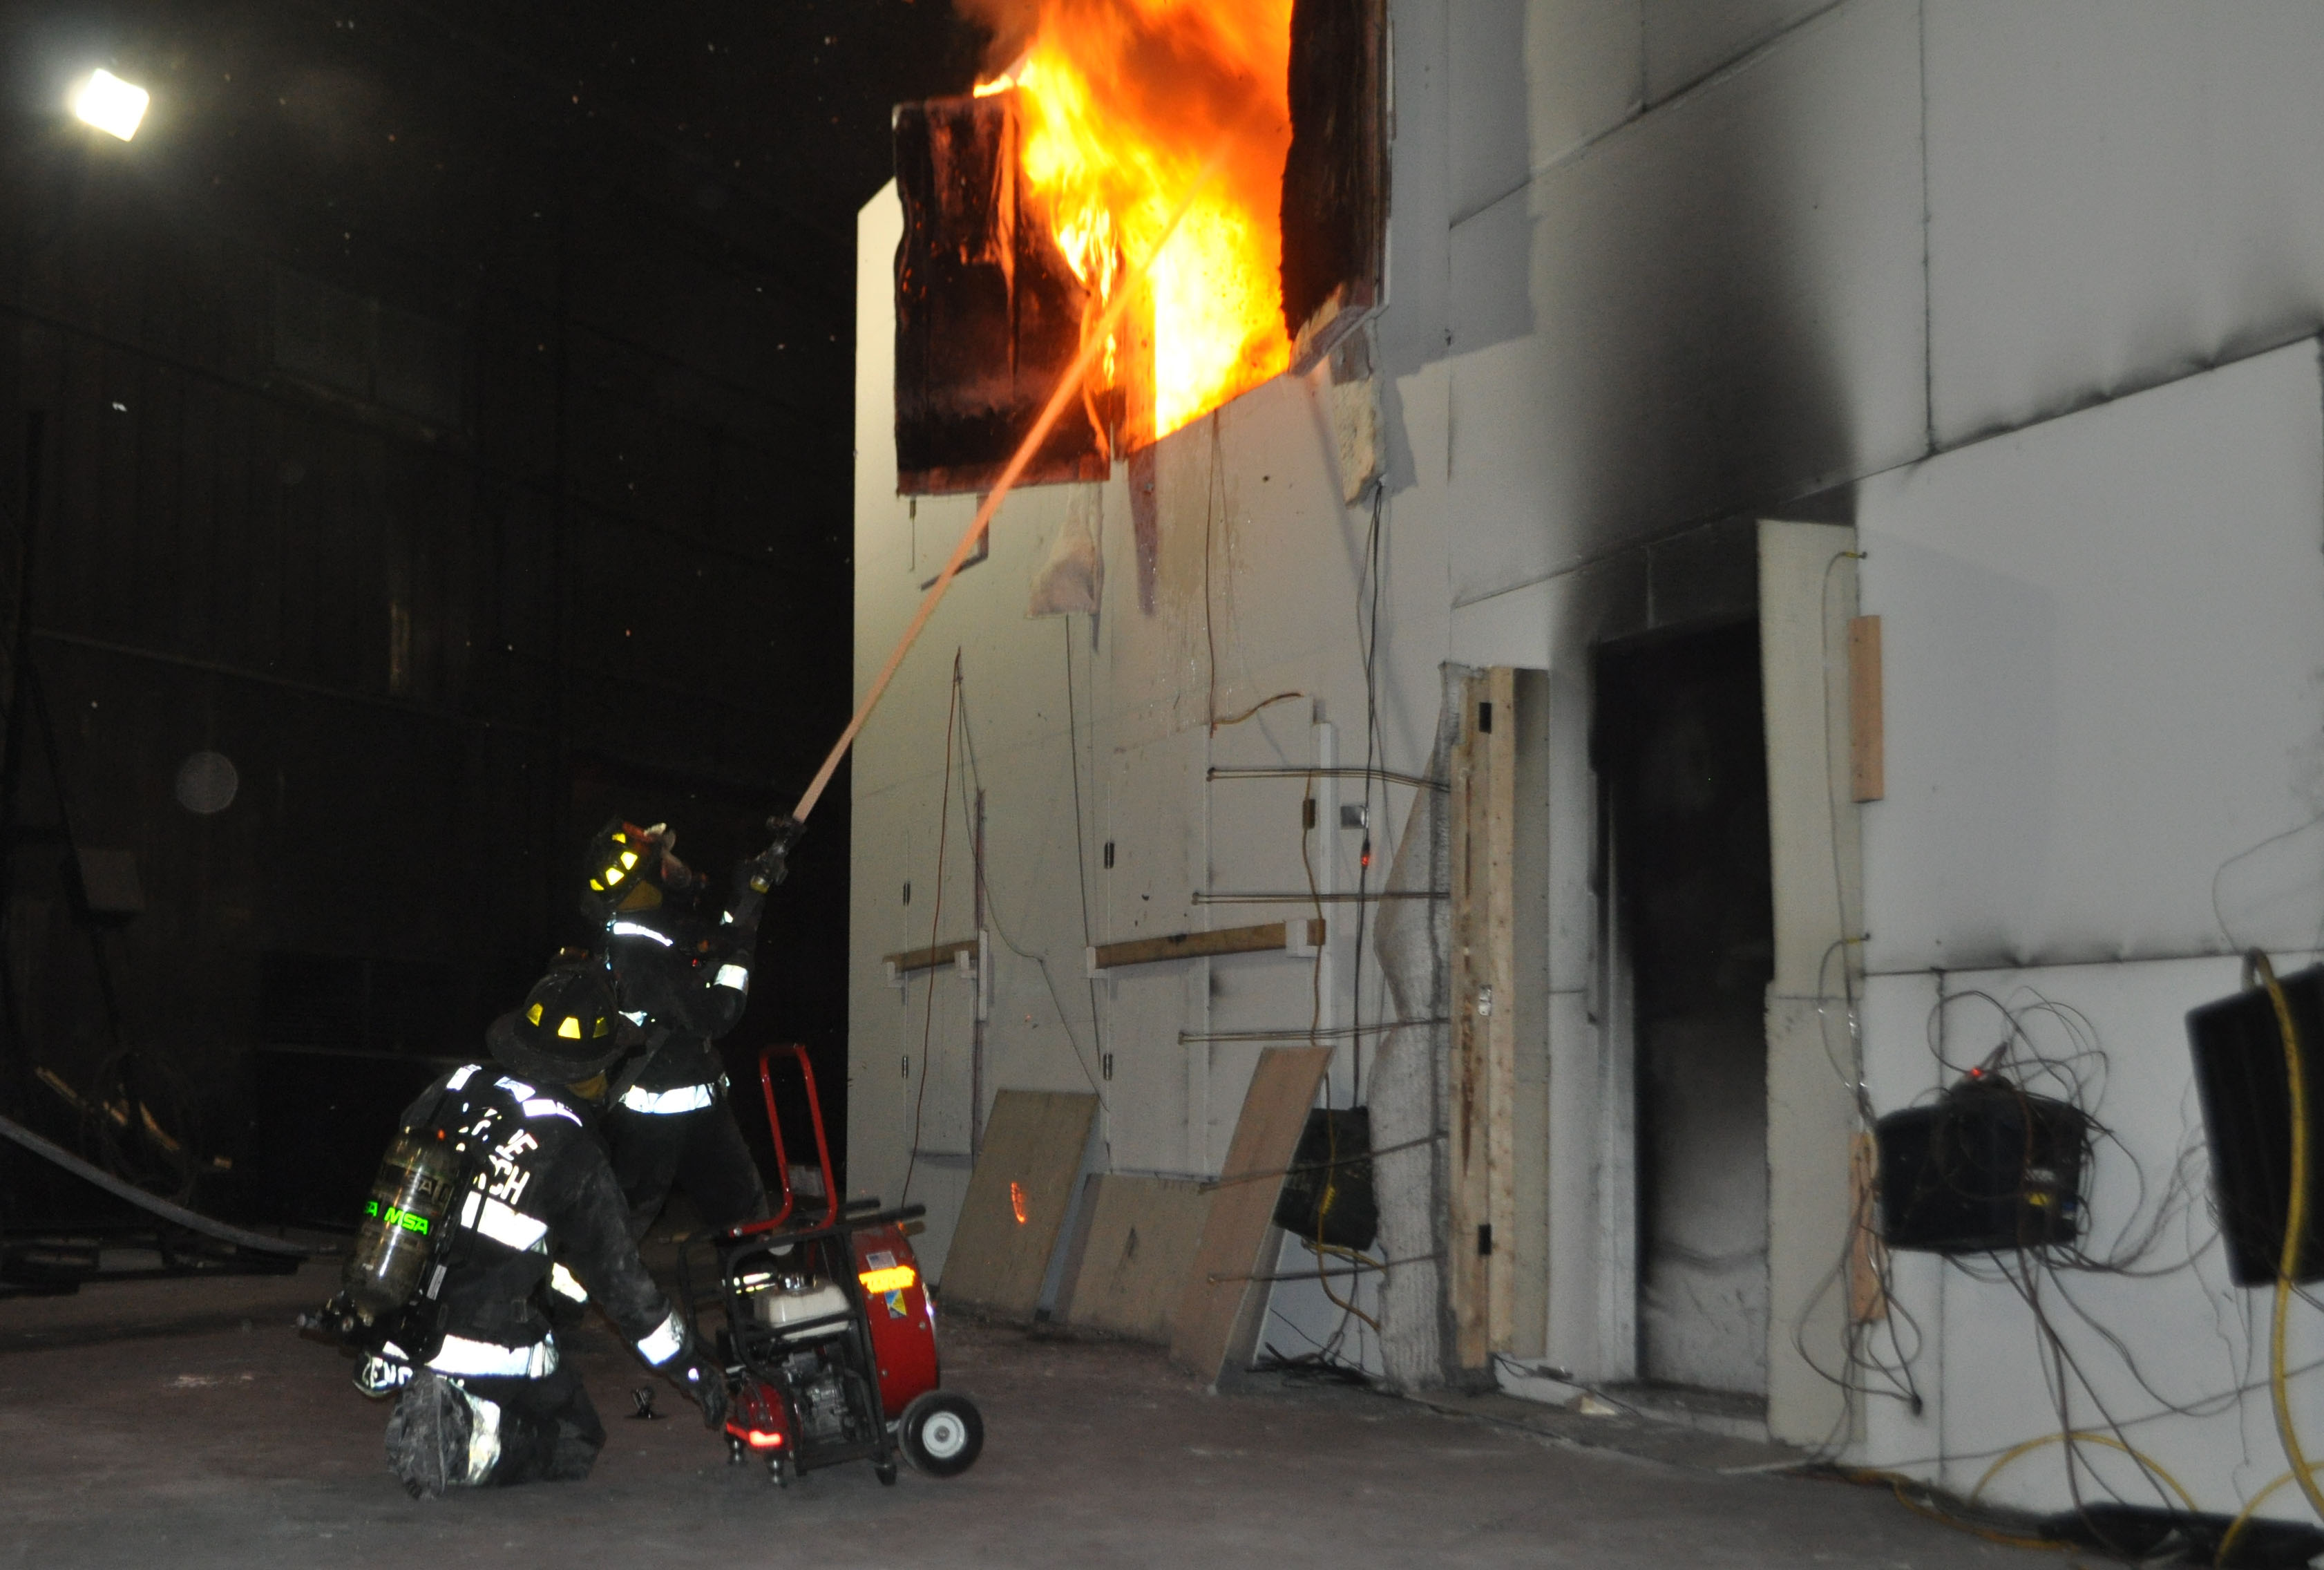
\includegraphics[width=7in]{0_Images/CoverImage.jpg}}}} 

			\vspace*{23\baselineskip} 

		\huge
		\begin{adjustwidth}{-0.5in}{-0in}
		\color{white}
		\textbf{Study of the Effectiveness of Fire Service \\ Positive Pressure Ventilation During Fire Attack \\ in Single Family Homes Incorporating Modern \\ Construction Practices\\}
		\end{adjustwidth}
		\begin{adjustwidth}{-0.5in}{}
		\color{white}
		\vspace{.2in}
		\large
		Robin Zevotek \\
		Research Engineer \\
		UL Firefighter Safety Research Institue \\
		\vspace*{\baselineskip}
		Stephen Kerber\\
		Director \\
		UL Firefighter Safety Research Institute \\ 
		\vspace*{\baselineskip}
		\today
		\vspace*{\baselineskip}
		\vspace{.2in}
		\begin{figure}[h]
			\hspace*{-0.5in}
\includegraphics[width=0.75in]{0_Images/Section_1/ULLogoWhite.pdf}
		\end{figure}
		\end{adjustwidth}
	\end{titlepage}

\clearpage

\begin{center}
DISCLAIMER\\
\vspace*{\baselineskip}
In no event shall UL be responsible to anyone for whatever use or nonuse is made of the information contained in this Report and in no event shall UL, its employees, or its agents incur any obligation or liability for damages including, but not limited to, consequential damage arising out of or in connection  with the use or inability to use the information contained in this Report. Information conveyed by this Report applies only to the specimens actually involved in these tests. UL has not established a factory Follow-Up Service Program to determine the conformance of subsequently produced material, nor has any provision been made to apply any registered mark of UL to such material. The issuance of this Report in no way implies Listing, Classification or Recognition by UL and does not authorize the use of UL Listing, Classification or Recognition Marks or other reference to UL on or in connection with the product or system.
\end{center}

\clearpage

\renewcommand{\abstractname}{Executive Summary}
\setlength{\emergencystretch}{5pt}

\begin{abstract}
There is a continued tragic loss of firefighter and civilian lives, as shown by fire statistics. One significant contributing factor is the lack of understanding of fire behavior in residential structures resulting from the use of ventilation as a firefighter practice on the fire ground. The changing dynamics of residential fires as a result of the changes in home construction materials, contents, size and geometry over the past 30 years compounds our lack of understanding of the effects of ventilation on fire behavior.  Positive Pressure Ventilation (PPV) fans were introduced as a technology to increase firefighter safety by controlling the ventilation.  However, adequate scientific data is not available for PPV to be used without increasing the risk to firefighters.

\noindent This fire research report details the experimental data from cold flow experiments, fuel load characterization experiments and full scale fire experiments. During the project it was identified that the positive pressure attack (PPA) and positive pressure ventilation (PPV) were often used interchangeably. For the purpose of this report they have been defined as PPA for when the fan is utilized prior to fire control and PPV for when the fan is used post fire control. 

\noindent The information from the full scale tests was reviewed with assistance from our technical panel of fire service experts to develop tactical considerations for the use of PPV fans in residential single family structures. A summary of these tactical considerations are as follows:

\noindent \bf{Understanding the Basics of Positive Pressure Ventilation/Attack} - \normalfont{An understanding of pressure, how pressure creates flow, and the how flow is associated with ventilation is essential to fully understanding PPA and PPV are either effective or in effective in ventilating a residential single family structure.} \\
	
\noindent \bf{Horizontal, Vertical and Positive Pressure Attack are different tactics.} - \normalfont{No one tactic will work in every scenario. Understanding the fire environment with emphasis on ventilation limited fire dynamics and how fire department operations impact those will ensure the tactic chosen is most effective.}\\
	
\noindent \bf{The setback of the fan or development of a “cone of air” is not as important as the exhaust size.} - \normalfont{In the application of PPA a great deal of emphasis has been placed on the flow occurring at the front door. Ensuring the "cone of air" does not equate to most effective flow. An aqueduct size exhaust is more important for creating the intended flow.}\\
	
\noindent \bf{During PPA, an ongoing assessment of inlet and exhaust flow is imperative to understanding whether or not a fan flow path has been established and if conditions are improving} - \normalfont{The fire attack entrance cannot tell you the conditions at the exhaust location(s). Assessing both the inlet, exhaust locations and interior conditions together provide the best assessment of PPA effectiveness.} \\
	
\noindent \bf{Positive Pressure Attack is Exhaust Dependant.} - \normalfont{For PPA to be effective the pressure created by the fan must be greater than the pressure created by the fire. Although fan size does play a role in the effectiveness of PPA, exhaust size plays a greater role. Providing enough exhaust to reduce the pressure in the fire room below what the fan is capable of producing in the remainder of the structure is essential for safe PPA operations.}\\
	
\noindent \bf{An outlet of sufficient size, must be provided, in the fire room to allow for effective PPA.} - \normalfont{PPA effectiveness is directly dependent on the ability of the fan to exhaust products of combustion to the exterior. Any exhaust opening created in conjunction with PPA should be located in the fire compartment.}\\
	
\noindent \bf{During PPA, creating additional openings not in the fire room will create additional flow paths making PPA ineffective with the potential to draw the fire into all flow paths.} - \normalfont{Additional openings not in the fire compartment, will lower the pressure in the adjacent compartments, allowing for more flow from the fire compartment to the remainder of the structure.}\\
	
\noindent \bf{The safety of PPA is decreased when the location and extent of the fire is not known with a high degree of certainty.} - \normalfont{To ensure the exhaust is provided in the most effective location it is essential to identify the location of the fire. Several indicators are available to aid firefighters in this identification such as heat signatures identified via thermal imaging cameras and smoke/neutral plane conditions.}\\
	
\noindent \bf{PPA will not be effective on a fire located in an open concept floor plan or any floor plan with high ceilings.} - \normalfont{In order for positive pressure attack to be effective, the fan must be capable of increasing pressure in the adjacent compartments. This forces the products of combustion out of the structure rather than into adjacent compartments. This pressure increase is only possible where the fire is located within a compartment.}\\
	
\noindent \bf{The application of water, as quickly as possible, whether from the interior or exterior prior to initiating PPA will increase the likelihood of a successful outcome.} - \normalfont{The application of water onto a compartment fire has been shown to slow the growth rate, increasing firefighter and occupant safety while decreasing property loss. This makes rapid hose line deployment a top priority for first arriving crews. Although positive pressure attack can improve the efficiency of a hose stretch, is not a substitute for the application of water on the seat of the fire. This early application of water will aid in the effectiveness of PPA.}\\
	
\noindent \bf{PPA is not a replacement for using the reach of your hose stream.} - \normalfont{Although PPA can reduce temperatures as crews approach a fire, it is not a replacement for the reach of a hose stream. Applying water as you approach the fire reduces the heat release rate making PPA most effective.} \\
	
\noindent \bf{During PPA, extension into void spaces is directly related to the exhaust capabilities of the void space.} - \normalfont{In order for fire extension into the void space there must be an entrance (penetration) for the fire and an exit(exhaust) for the products of combustion to leave.} \\
	
\noindent \bf{PPA does not negatively affect the survivability of occupants behind a closed door.} - \normalfont{Prior research shows the importance of having a closed door between occupants and the fire if they are unable to escape.  These PPA experiments reinforced this assessment as temperatures and gas concentrations in the closed or isolated rooms remained tenable while conditions in open compartments exceeded tenability thresholds.}\\
	
\noindent \bf{When PPV is used, in single story residential structures, the more openings made in the structure during PPV (Post Knockdown) the more effective it is at ventilating the structure.} - \normalfont{The 18 in. gas fan used was capable of moving so much air it could exhaust through more than 5 times the inlet size to most efficiently remove products of combustion. As the number of exhaust points increased the exhaust flow continued to increase. The greater the exhaust flow, the faster the structure was ventilated.} \\
	
\noindent \bf{When PPV is used, it is important to assess for extension.} - \normalfont{While the fan provides additional visibility afterfire control by exhausting products of combustion out of the structure faster, it also has the potential to hide extension in void spaces. Directing attention to these spaces immediately following knockdown will limit the possibility of extension.}\\

\noindent \bf{When PPV is used, starting or turning in the fan immediately after fire control will provide the most benefit.} - \normalfont{Once water is on the fire and the attack crew has the upper hand, fans will assist with increasing visibility and reducing temperatures to ambient to allow for other fire ground operations like search, rescue and overhaul to happen faster and more efficiently. The use of the fan must be coordinated with interior crews and incident command to ensure re control has been achieved.}\\

\end{abstract}

\newpage

\tableofcontents

\newpage

\section*{Introduction}
The purpose of this study is to increase firefighter safety by providing the fire service with credible scientific information, developed from full-scale fire testing in representative modern single family homes, on the usage of positive pressure ventilation fans during fire attack. 

\clearpage

\section{Background}
NFPA estimates \cite{NFPAFireLoss} that from 2002-2011, U.S. fire departments responded to an average of 398,000 residential fires annually. These fires caused an estimated annual average of 2,820 civilian deaths and 13,780 civilian injuries. More than 70\% of the reported home fires and 84\% of the fatal home fire injuries occurred in one- or two- family dwellings, with the remainder in apartments or similar properties. For the 2006-2009 period, there were an estimated annual average 35,743 firefighter fire ground injuries in the U.S. \cite{NFPAFFInjuries} The rate of traumatic firefighter deaths occurring outside structures or from cardiac arrest has declined, while at the same time, firefighter deaths occurring inside structures has continued to climb over the past 30 years. \cite{NFPALast30} Ventilation is believed to be a significant contributing factor to this continued climb in firefighter injuries and deaths. Developing the proper knowledge about the use of PPV will enable more departments to implement its use with the confidence of knowing when to apply it to increase the safety of their members, whether in place of or supplementing current ventilation tactics.

Over the last 5 years of fire service research, it has become clear that the fire service needs more information and knowledge about fire dynamics and how the changing fire environment impacts their tactics and safety. Studying the modern fire environment has shown that fires grow faster today than ever before, they become ventilation limited (or run out of air) and the control of that air during fire attack is critical to a safely mitigated fire incident \cite{ChangingResdFires_Kerber}. Two previous UL studies have examined horizontal ventilation \cite{One_Two_Family_Fires_Kerber} and vertical ventilation \cite{UL_VerticalVent} which are the two most common types of ventilation used by the fire service on a daily basis. The results of these studies have been disseminated to the fire service with positive feedback \cite{HowToKeepFirefighterSafer_Goldfeder}, \cite{SurbarbanFirefighting_Knapp} regarding the integration of tactical considerations into their standard operating procedures. The fire service anticipates increased safety due to the knowledge obtained from UL’s research as they better understand the necessary coordination of ventilation and suppression. Following each presentation on the horizontal and vertical ventilation results, firefighters have also consistently sought similar data and knowledge for the use of positive pressure ventilation (PPV). 

PPV is a technique used by the fire service to remove smoke, heat and other combustion products from a structure. This technique uses a fan or multiple fans to create a higher pressure inside the home in order to speed up the flow to the lower pressure outside of the house (Figure \ref{fig:PPV_Diagram}). This allows the fire service to perform tasks within the structure in a more tenable atmosphere. Since it was introduced in the 1980’s, PPV has become an important tool in the fire service. Many departments have adopted this technique after water has been applied to the fire to assist in the overhaul phase of the fire. Several other departments have incorporated it as part of their initial fire attack. When used during fire attack, a PPV fan or blower is placed at the entry point of the attack crew and air is forced through the home and out through an exhaust point ahead of the crew. Under ideal conditions, visibility is increased as smoke and heat are forced ahead of the attack crew and away from occupants inside. This makes the fire attack, search, and other fire ground operations easier and safer to complete.


\begin{figure}[H]
	\centering
	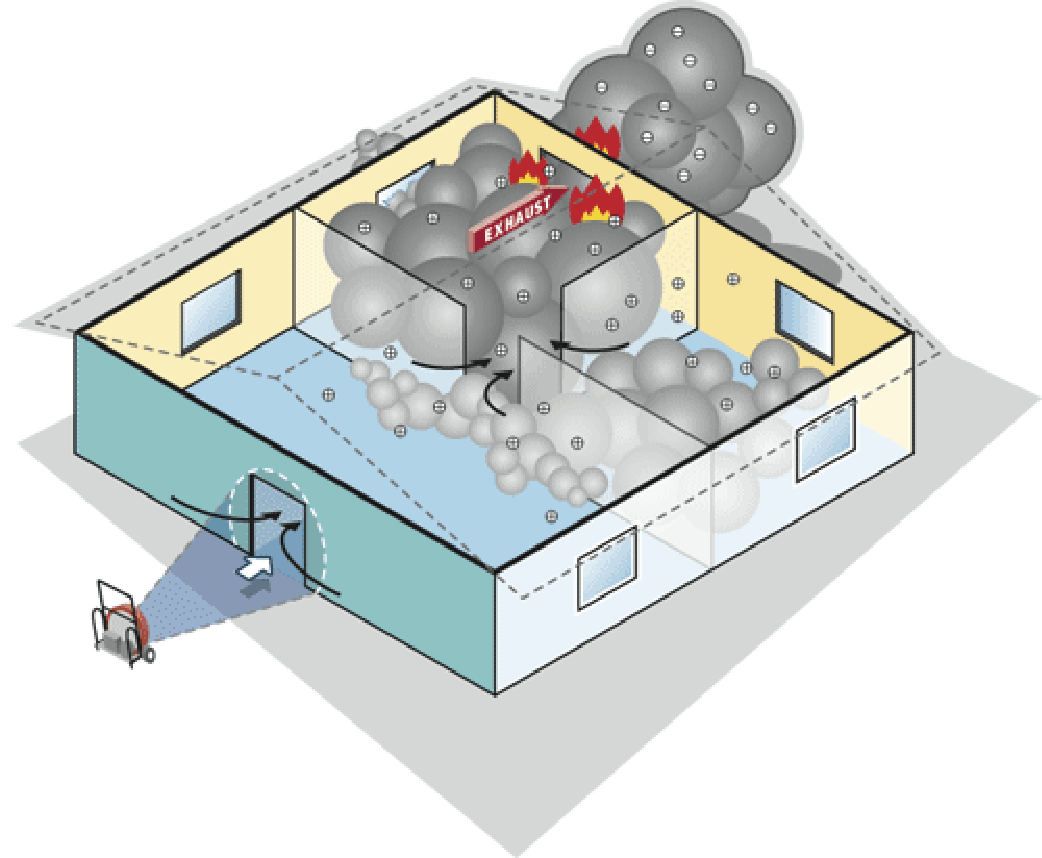
\includegraphics[width = 4in]{0_Images/Tactical_Considerations/Exhaust_Over_Cone/ppv_illistration.pdf}
	\caption{Diagram showing the basic application of positive pressure ventilation}
	\label{fig:PPV_Diagram}
\end{figure}

Since its PPV has become an important tool in the fire service, yet its use is polarizing. Some departments have developed confidence in using PPV, citing its positive impact on firefighter safety. A majority of departments refuse to use PPV because of the uncertainty created by the unanswered questions above or a negative experience with the technology. Constrained by current economic conditions, many departments have limited staffing or have had their staffing reduced and are experimenting with ways to utilize technologies such as positive pressure ventilation fans during fire attack. However, risks exist when it use is not accompanied by appropriate scientific investigations or post-release surveillance of the impact on firefighter and occupant safety. There have been incidents where PPV has been incorporated into firefighting tactics without developing a scientific basis of their use. The lack of knowledge has led to improper usage, misapplication, and numerous injuries and line of duty deaths \cite{NIOSHF2000-44} \cite{NIOSH98F-32} \cite{TexasFMFY07-02} \cite{ContraCostaFalaityInvestigation} \cite{NIOSHF2004-02} \cite{NIOSHF2002-12}. These referenced reports detail the circumstances under which firefighters lost their lives and in each of these cases a PPV fan was in operation. In most of the incidents, it is not clear what role the PPV may have played due to the complexity of the incident and many simultaneous actions. 

Some fire departments have utilized PPV fans after water was applied to the fire but prior to fire control. In these situations, it was observed that fire will intensify while a fan is being used as is expected with additional oxygen made available by the fan. Fire service training on the proper use of fans and their impact on fire dynamics has been difficult. Fire service training buildings are not able to safely replicate the ventilation limited fire conditions needed to understand the impact of PPV. That limitation is combined with the safety requirement to use wood based fuels in training which does not replicate the speed or magnitude in which a fire grows, spreads, and reacts to the oxygen added by the PPV fan. This same requirement is placed on acquired structure burn training as well. So even if realistic home geometries become available, the fire service is not able to use realistic fuels such as sofas, per NFPA 1403 (the Standard on Live Fire Training Evolutions). There has also been an incident (see Figure \ref{fig:PPVTrainingInj}) where firefighter instructor and trainee have been injured from improper use of PPV techniques \cite{LasVegasNews_ChiefsRole}. This underlines the need for developing scientific data that can be used both on the fire scene as well as during firefighter training.

\begin{figure}[H]
	\centering
	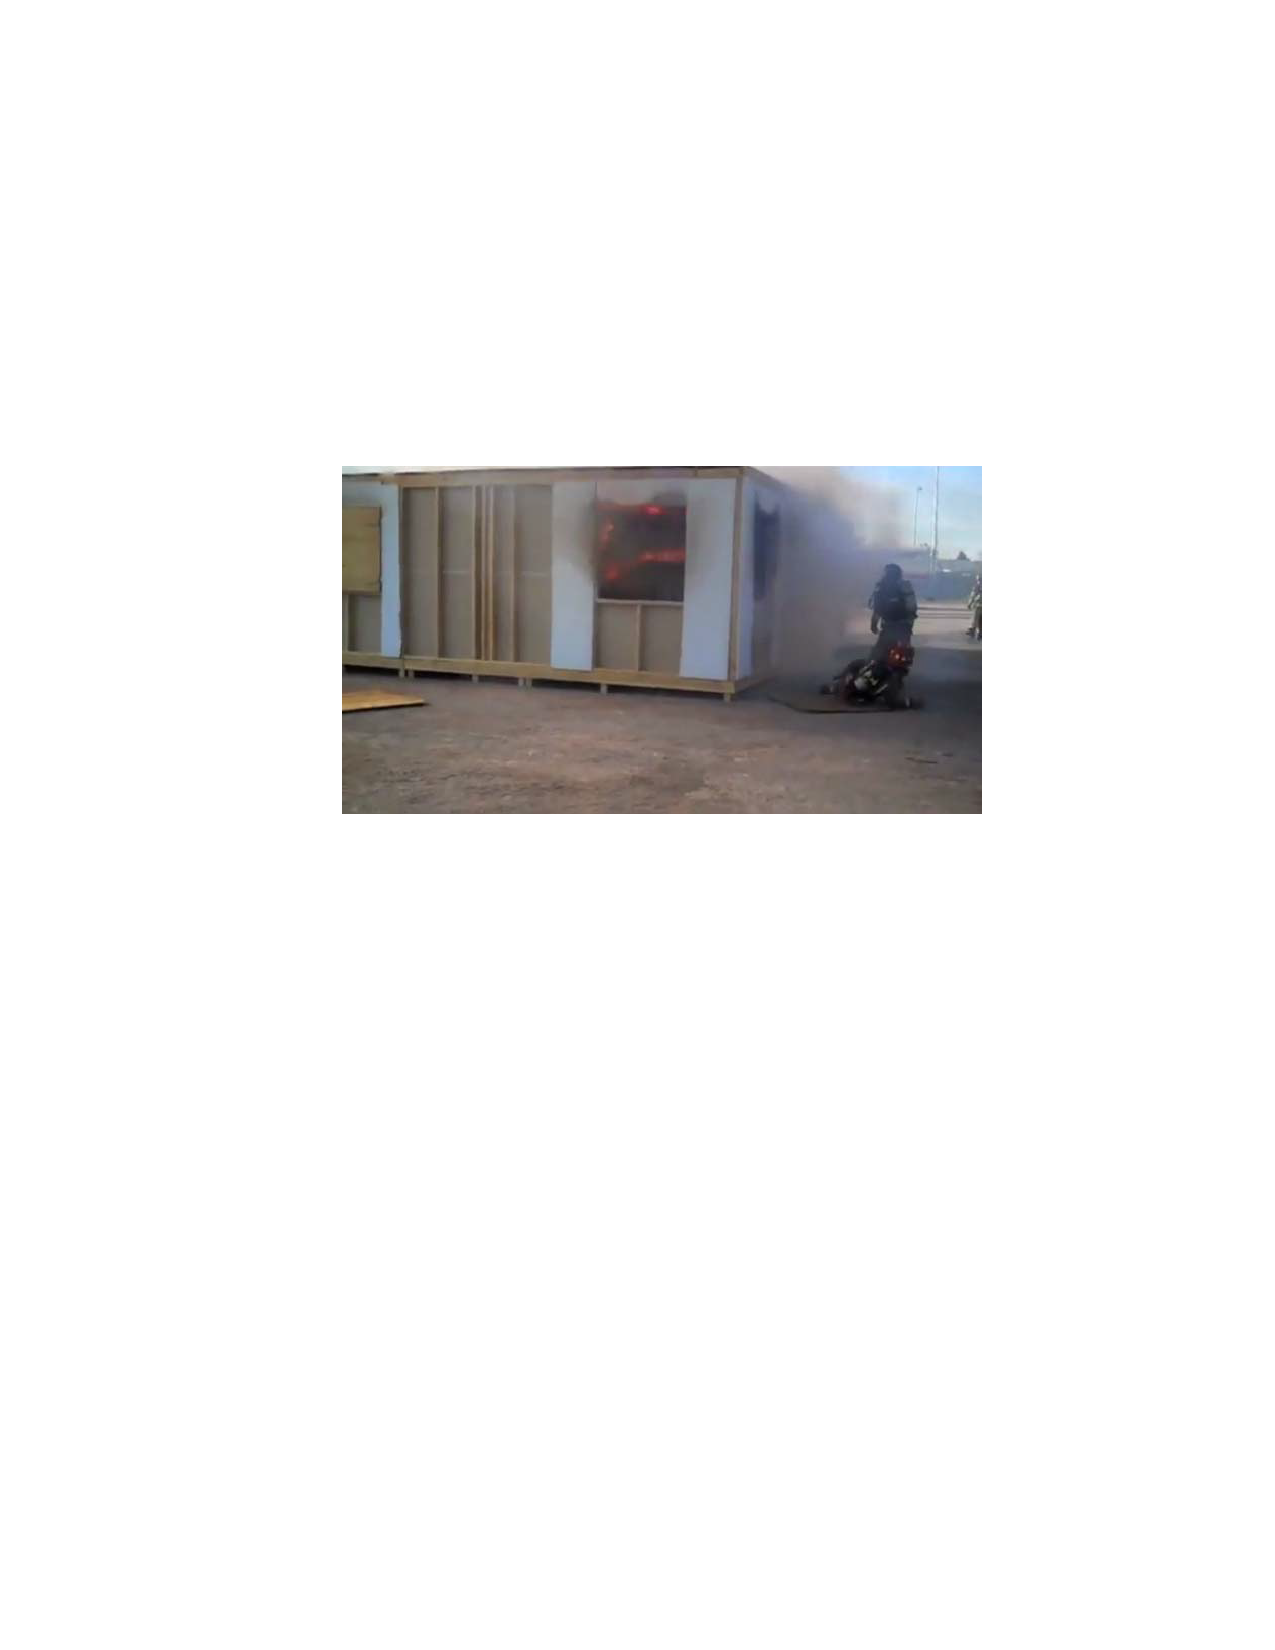
\includegraphics[width = 5in]{0_Images/Background/PPVTrainingInjury.pdf}
	\caption{Moments after lead instructor and student jump out of window to escape further injury during PPV training exercise}
	\label{fig:PPVTrainingInj}
\end{figure}

The use of PPV must be coordinated with fire attack and timed with other ventilation procedures. Traditionally this is done by an interior crew with the fan flow at their back. However, reduced staffing at fire departments have led to firefighters attacking the fire by applying water from outside the structure. A concern with this practice is that applying water externally will “push fire” into the house and subsequently decrease the tenability of occupants inside the structure. Further, since PPV provides additional oxygen to the fire and can increase the rate of heat released. This can easily exacerbate firefighting operations if the ensuing fire dynamics are not fully understood. Thus, use of PPV needs to be optimized in the overall context of firefighter tactics such as horizontal and vertical ventilation, deployment of firefighter teams, and timing of the use of PPV.

Key factors that need to be addressed to implement PPV safely and most effectively include
the following:

\begin{itemize}
	\item Impact of home structure on PPV effectiveness.
	\begin{itemize}
		\item Home Size
		\item Floor Plan
		\item Void Spacees (e.g attic)
		\item Fuel load
	\end{itemize}
	\item Impact of PPV tactic on fire dynamics.
	\begin{itemize}
		\item Potential of increased hazards associated with forcing fire gases into the eave or attic space.
		\item Potential of blowing fresh air pushing fire through a house or spreading fire from a non-vented room to a vented room.
		\item Impact to occupants (and fire teams) that are in or out of the flow path and may be downstream of the fan.
		\item Conditions created when the flow path to the exhaust is blocked inside the structure.
		\item Transition from a content to a structure fire by forcing hot gases into void spaces.
	\end{itemize}
	\item Integration of PPV with other ventilation techniques
	\begin{itemize}
		\item Comparison to natural horizontal ventilation tactics and development of optimized firefighting ventilation tactics.
		\item Potential hazards associated with commencing PPV while fire attack crews are inside the structure.
	\end{itemize}
	\item Impact of PPV technology and parameters on effectiveness.
	\begin{itemize}
		\item Fan flow rate
		\item Size of exhaust opening and the ideal inlet/exhaust ratio.
		\item Influence the location of exhaust or openings
	\end{itemize}
\end{itemize}

Research organizations and the fire service have made significant contributions to understanding the scope and limitations of the use of the PPV in fire scenarios over the past two decades. However, there are several gaps that limit its use by the fire service. These may be categorized as follows: (i) type of structures used in the research; (ii) fuel loads; (iii) fire ventilation conditions; and (iv) PPV parameters considered. There are further discussed herein. \par

\textbf{Fire Test Structures:} In many studies, fire department training buildings have been used in the experiments. These buildings are typically constructed with metal or concrete walls that absorb energy differently from representative single-family homes \cite{HughesPPVTesting} \cite{KerberPPVinTraining} \cite{SvennsonFireVentilationDuringOperatoins}. 

\textbf{Fuel loads and Fire Ventilation Conditions:} Some of the studies were limited to wood based fuels (e.g., wood pallets, straw). These fuel sources have different burning characteristics than fuel sources (e.g., upholstered furniture, mattress, carpets, stored items, etc.) in representative single family homes in the USA. Thus, findings from these studies \cite{HughesPPVTesting} \cite{KerberPPVinTraining} \cite{SvennsonFireVentilationDuringOperatoins} have limited practical applications for firefighting tactics. \par

In some studies, fuel packages were utilized which do not allow for the realistic ventilation limited fire conditions necessary to make conclusions that are expected in actual incidents \cite{ExekoyePPVHouseFires} \cite{SvenssonFireVentinLargeFireHall} \cite{BowserTacticalVent} \cite{EzekoyePPVStrucuresReport}. These referenced studies utilized stacks of wooden pallets, foam racks with limited amounts of foam, gas burners, or small pans of flammable liquids. These fuel loads are easily repeatable and cost effective, but again limit the practical application of the results. In the absence of ventilation limited conditions, the impact of added oxygen can only improve conditions, which may be misleading to the effects encountered at actual incidents. Some studies have used computational and scale fire modeling due to the high cost of fire testing but have not been validated, and therefore not incorporated into operating procedures \cite{Didona1993modeling} \cite{KerberPPVCFD} \cite{KerberPPVFDS} \cite{TuomisaariVentilationInFirefighting}. \par

\textbf{PPV Parameters:} \mbox{}Additional studies examined the use of PPV fans in large structures and high-rise buildings \cite{SymposiumHighRisePPV} \cite{KerberMadrzyPPVInLargeStructures} \cite{KerberMadrzyPPVInHighRise}. The results of these studies have added to the understanding of the scope and limitations of PPV. However, in most cases, these studies examined the fan’s ability to pressurize areas of a building to limit fire and smoke spread, which is very different than blowing air through the fire compartment in a one and two family home. 

Since the initial introduction of fans into the fire service, newer fan technologies have been developed (including conventional, turbo and Pow’Air). These technologies have not yet been investigated in realistic fire scenarios. Also, fan manufacturers have increased flow rates over time. When first introduced, most fans were rated at less than 10,000 cubic feet per minute (CFM); now similar sized fans are rated in excess of 30,000 CFM. The impact of forcing more air into a house fire is not well understood. PPV fans can be found on apparatus around the world and are available in many shapes and sizes. There are portable fans as small as 16 in. and truck mounted fans as large as 60 in. They are powered with gasoline, electric, hydraulic, battery and propane motors. Gasoline powered are the most common, but are accompanied by additional concerns about carbon monoxide (CO) production. Some research has been done on this topic, but CO measurements will be made during these experiments to add to the body of knowledge 39,40. 

This study used representative modern and traditional home geometries, realistic fuel loads representative of furnishings found in today’s homes, fan technologies, sizes and ratings available to the fire service today and simulated response and operational times in order to adequately address the questions and concerns the firefighter community has expressed. In addition it is intended to provide a baseline for choosing when and when not to employ PPA or PPV on the fireground. The results and conclusions of this study are intended to be used to improve firefighting tactics, fire ground safety and fire dynamics knowledge \cite{KerberMadrzyPPVInHighRise} \cite{LougheedPPVHighRise}.

\clearpage

\section{Objectives and Technical Plan}

\subsection {Objectives}

The purpose of this study was to increase firefighter safety by providing the fire service with credible scientific information, developed from full-scale fire testing in representative modern single family homes, on the usage of positive pressure ventilation fans during fire attack. This was accomplished with the completion of the following objectives:

\begin{itemize}
	\item Improve firefighter safety by increasing knowledge of fire behavior.
	\item Develop knowledge of positive pressure ventilation tactics.
	\item Identify and disseminate standard best practices for the use of positive pressure ventilation during fire attack based on science.
	\item Provide the knowledge to better understand the fire dynamics and building response factors may mitigate fireground injuries and fatalities through the use of positive pressure ventilation fans during fire incidents.
	\item Generate understanding of modern construction practices such as open floor plans and great rooms on positive pressure ventilation tactics.
	\item Bring the ‘Science to the Streets’ by transferring science based tactical considerations founded on experimental results that can be incorporated into firefighting standard operating guidelines.
\end{itemize}

All five of the Technology \& Fire Service Science issues facing the fire service determined during the 2nd National Fire Service Research Symposium \cite{NFFF} were incorporated into this study.

\subsection{Technical Plan}

This study consisted of the following tasks:

\begin{figure}[H]
	\centering
	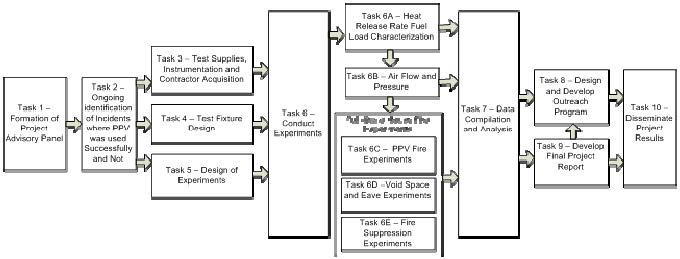
\includegraphics[width = 6in]{0_Images/Objectives_and_Technical_Plan/DHS2012_TechnicalPlan_FlowChart.jpg}
	\caption{Project Technical Plan Flow Chart}
	\label{fig:TechPlanChart}
\end{figure}

\begin{itemize}
	\item \textbf{Task 1 – Formation of a Project Advisory Panel} \\ 
	Task 1 brought together an advisory panel of technical experts in the fire service; fire service research field and PPV fan manufacturers. The panel included fire department representatives from departments that use positive pressure ventilation during fire attack and from departments that stopped using it or wish to use it. 
	
	\item \textbf{Task 2 – Incident Review} \\
	Task 2 involved conducting an extensive search to find as many incidents as possible where PPV was used successfully or unsuccessfully during fire attack. This was completed by conducting interviews with departments that are known to have standard operating procedures for the use of PPV, or previously used PPV during fire attack but stopped for various reasons from the technical panel in developed in task 1. Common trends, successes and failures, and concerns were documented and shared with the technical panel for the development of the experimental series. 
	
	\item \textbf{Task 3 – Test supplies, Instrumentation and Contractor Acquisition} \\
	In Task 3 UL acquired research supplies and instrumentation to complete the project. Instrumentation included thermocouples to measure thermal conditions that potential victims or firefighters could be exposed to, differential pressure sensors and bidirectional probes to measure pressure and gas velocity throughout the test fixtures, bullet cameras to capture interior views of the test fixtures to provide visual evidence of conditions. Other test equipment such as data loggers, gas analyzers, thermal imaging cameras and video cameras were acquired from previous studies and were utilized during this study. A contractor was also selected to construct the test house structures using construction practices representative of what is found in most neighborhoods across the country.
	
	\item \textbf{Task 4 – Test Fixture Design} \\
	Task 4 was the design of the test fixtures to be used in the experiments. The main test fixtures, two single family residential homes (1-1200ft$^2$ single story ranch house and 1-3200 ft$^2$ two-story colonial house), were constructed in UL’s Large Fire Facility. These were the same designs built for the two previous ventilation research grants and therefore allowed continuity of previous results to expand our knowledge.
	
	\item \textbf{Task 5 – Design of Experiments} \\
	Task 5 was the design of the experiments. In this task UL’s project engineers worked work closely with the technical panel to ensure fire service concerns were addressed and that the results were of great benefit to the end users. All experimental variables, equipment, personnel, infrastructure and other resources were evaluated to determine the best set of experiments to get the most for the investment and provide the largest return to the fire community. Variables included fan size, placement, technology, ventilation parameters, timing of tactics, ignition location, and fuel loading
	
	\item \textbf{Task 6 - Conduct Experiments} \\
	\begin{itemize}
		\item \textbf{Task 6A: Heat Release Rate Fuel Load Characterization} \\
		Methodology: Conduct heat release rate (HRR) experiments under the 10MW calorimeter in UL’s Large Fire Facility. This allowed the team to characterize modern furnishings and to understand the heat release of today’s fire environment. This also quantified the fuel load used for the remainder of the experiments which were designed to have a similar HRR curve and total heat released as the two previous ventilation studies.
		\vspace{\baselineskip}
		Measurements: Heat release rate measured via oxygen consumption calorimetry, temperature utilizing thermocouples placed in an array within the room, video and thermal imaging cameras will be used to document the fire spread.
		
		\item \textbf{Task 6B: Air Flow and Pressure Experiments} \\
		Methodology: Conduct air flow and pressure experiments in the test fixtures prior to the introduction of any fire. Variables that were characterized during this series of experiments were fan technology (shrouded, jet, turbo), fan placement (setback from the doorway and angle), impact of inlet and outlet sizes and ratios, and impact of volume between the houses. These tests will provide the baseline of flows created with the fan alone and will be compared to the same data taken during the fire experiments in the following tasks.
		\vspace*{\baselineskip}
		Measurements: During each of these experiments, velocities were measured with bidirectional probes attached to differential pressure transducers in conjunction with thermocouples and pressures were measured with differential pressure transducers.
		
		\item \textbf{Task 6C: Full-Scale PPV House Fire Experiments} \\
		Methodology: Conduct a series of 25 full-scale house fire experiments examining fire service PPV tactics. Two full scale test house structures were constructed in UL’s large fire facility; the structures used the same floor plan design as used in previous research on fire service horizontal ventilation tactics (EMW-2008-FP-01774)\cite{DHS2008} and vertical ventilation tactics (EMW-2010-FP-00661)\cite{DHS2010}. These experiments provided the scientific basis necessary to begin to fill the knowledge gap that exists regarding the proper usage and limitations of this tool and tactic. Sections \ref{SingleStoryExp} and \ref{TwoStoryExp} detail the 25 experiments conducted.
		\vspace*{\baselineskip}
		Measurements: Both houses were instrumented to measure temperature in every room, gas concentrations, pressure, gas velocity, thermal imaging and digital video. These measurements allowed for quantification of fire behavior, the impact of the positive pressure ventilation tactic and tenability for firefighters and occupants.
	\end{itemize}
	\item \textbf{Task 7 – Data Compilation and Analysis} \\
	Task 7 was the compilation and analysis that was conducted by UL engineers to make the data usable by the fire community. The data was organized in graphs that were reviewed by the technical panel in preparation for the final report and the online training program. In addition, tactical considerations were developed in conjunction with the fire service technical panel. Each of these considerations are supported by data and video evidence and incorporated in the technical report and outreach program.
	
	\item \textbf{Task 8 – Design and Develop Outreach Program} \\
	In task 8, UL engineers worked with instructional designers to produce an interactive training program for the fire community. The final program is shared via UL FSRI's website free of charge.  The course contains data, pictures, video and professional narration and allowing firefighters of all levels to navigate through the course at their own speed. This program highlights linkages to tactical considerations learned from the previous two studies on horizontal and vertical ventilation.
	
	\item \textbf{Task 9 – Develop Final Project Report} \\
	Task 9 was development of this final report that details all of the experiments and results. This report which has been provided to DHS and made publicly available via UL FSRI' website will serve as a reference for future research. The tactical considerations developed with the support of the technical  panel make up the majority of this report.
	
	\item \textbf{Task 10 – Disseminate Project Results}
	Task 10 involved the dissemination of the research results. Results are continiously shared by presenting in venues such as the National Fire Protection Association Annual Conference, Fire Department Instructors Conference, International Association of Fire Chiefs Fire Rescue International, and the International Association of Fire Fighters Annual Conference. These venues provide a large number of attendees from the fire service and research communities and are a formal means to disseminate the results of the study. Additional dissemination is provided via publication in fire service trade magazines and peer reviewed journals. As with previous outreach results, videos and presentation content will be made available at request to be used for local dissemination and for train the trainer programs. 

\end{itemize}

\subsection{Limitation and Scope}

The purpose of this study is not to establish if positive pressure attack or positive pressure ventilation are more effective than other types of ventilation. The purpose is to increase the fire service’s knowledge of the impact of these tactics under specific conditions. Since all fireground circumstances cannot be analyzed, it is anticipated that the data developed and this analysis will enable firefighters to complement their previous observations and experiences.

Every fire event that the fire service responds to is unique. The range of fire ground variables at each fire event make firefighting complex. In this investigation, key variables were identified and bounded to develop the data under controlled conditions. These variables included:

\begin{itemize}
	\item House geometry.
	\item Hosue Construction.
	\item Fuel loading. 
	\item Fire department arrival time. 
	\item Tactical choices.
	\item Hose stream flow rates.
	\item Fan (manufacturer and model...at least in the live fire experiments)
	\item Fan placement.
	\item PPA inlet/exhaust locations. 
\end{itemize}

In order to allow for a consitant comparision of tacticiacl choices no glass windows were utilized. Windows were replaced with plugs constructed of framing lumber covered with a cement board to represent the window. This prevented unintended glass failure which had the potential to occur in an inconsistant manor.  

By bounding these variables and controlling the test conditions during firefighting operations, the impact of positive pressure attack and fire suppression tactics on fire dynamics and conditions in two types of single family homes was examined. The results enable the establishment of a scientific basis that may be used for other types of structures that are different sized rooms, different fuel loads, different interior geometries, different timing of operations, etc however have the same architectural features. This work was not intended to examine positive pressure attack or positive pressure ventilation in other than single family homes. The test structures included a single family, 1200ft2 ranch home and a 3200ft2 two story open concept floor plan home. Extrapolation of the scientific basis established in this work would not be applicable in multi-family, commercial or industrial facilities. 

The fires in this study, where positive pressure attack was used, were content fires and represented a fire event within the living space of the home, and not a structure fire with fire extension into the wall, floor and/or attic spaces. These experiments were also meant to simulate initial fire service operations by an engine company or engine and truck company arriving together in short order within the range of national average response times of less than 8 minutes \cite{USFA_Response_Times}.  

The structures used represent common residential structures found throughout the U.S. A modern two story open floor plan and a single story ranch structure representative of smaller compartmentalized home. The structures were built such that they will accurately represent Type V (wood frame) construction allowing the results to be analyzed and used to develop residential structure fire tactical considerations. 

\clearpage

\section{Project Technical Panel}

A project Technical Panel was established of fire service personnel from all over the world. In an effort to ensure subject matter experts with a wide array of experience an application was developed with an application period lasting 60 days. Over 90 applications were received and reviewed by UL's Firefighter Research Institutes team for training level and experience with positive pressure attack and ventilation. Additionally panel members were evaluated based on rank and geographical location to develop input from all ranks and geographical areas. The final 25 technical panel members were selected to most accurately represent a cross section of firefighters who have either used or are using positive pressure attack and ventilation. 

\begin{figure}[H]
	\centering
	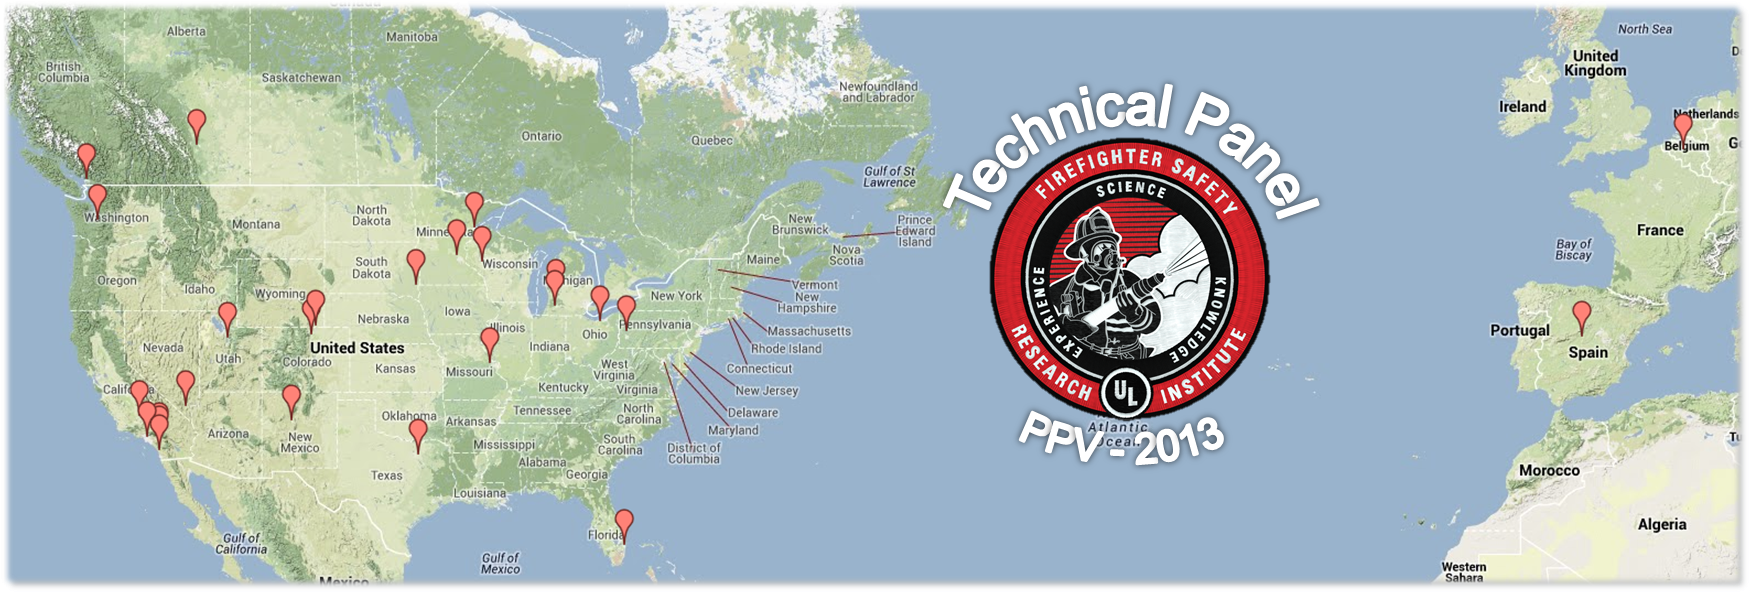
\includegraphics[width = 5in]{0_Images/Technical_Panel/TechnicalPanelLocations.png} 
	\caption{Positive Pressure Attack Technical Panel Member Locations}
	\label{fig:PanelLocatoins}
\end{figure} 

The individuals below provided direction for the project, assisting in planing the experiments, witnessing the testing and developing tactical considerations. Their tireless support and effort make this project relevant to the fire service across the world. 

\renewcommand{\arraystretch}{1.5}

\begin{table}[H]
	\centering
	\caption{Fire Service Technical Panel}
	\begin{tabular}{|c|c|}
		\hline
		\bf{Name} & \bf{Fire Department} \\ \hline \hline
		Art Armalich & CERN Labs Fire Department \\ \hline
		Jason Bennett & Proude Fire Authority \\ \hline
		Ian Bolton & North Vancouver District Fire Services \\ \hline
		Jason Caughey & Laramie County Fire District \\ \hline
		Scott Corrigan & Pierce County Fire Department \\ \hline
		David Downey & Albuquerque Fire Department \\ \hline
		Chip Everett & Oshtemo Township Fire Department \\ \hline
		John Flynn & Palm Beach County Fire Rescue \\ \hline
		Adam Frick & Sioux Falls Fire Department \\ \hline
		Kriss Garcia & American Fork Fire Department \\ \hline
		Gregg Gerner & General Motors Assembly \\ \hline
		Jeff Gillette & East Valley Fire Department \\ \hline
		Jim Golondzinier & Los Angeles County Fire Department \\ \hline
		Andy Golz & Duluth Fire Department \\ \hline
		Dennis Haisma & Grand Rapids Fire Department (Ret.) \\ \hline
		Josh Janssen & Riverside County Fire Department \\ \hline
		Tom Jenkins & Rogers Fire Department \\ \hline
		Brian Kazmierzak & Penn Twp Fire Department \\ \hline
		Colin Kelley & Clark County Fire Department \\ \hline
		Karel Lambert & Brussels Fire Department \\ \hline
		Nick Ledin & Eau Claire Fire Department \\ \hline
		Scott Lindsay & Calgary Fire Department \\ \hline
		Joseph Pronesti & Elyria Fire Department \\ \hline
		Garrett Rice & Colony Fire Department \\ \hline
		Ned Vander Pol & Vista Fire Department \\ \hline
	\end{tabular}
	\label{tab:TechPanelList}
\end{table}

\clearpage

\section{Previous Literature}
A literature review was conducted to identify previous work, current tactics and knowledge gaps as it relates to the use of positive pressure fans for residential fire attack. This section details the work found in fire service publications, fire service training manuals, firefighter line of duty death reports and past research projects. This is not intended to be an all encompasing review, only to highlight the current litureature available on the use of positive pressure fans. 

\subsection{Fire Service Publications}

\subsection{Fire Service Training Manuals}



\subsection{Firefighter Line of Duty Deaths}
The following is a brief summary of the National Inisiture of Occupantional Health Firefighter Line of Duty Death and close call incidents involcing the use of positive pressure fans: 

\begin{itemize}

\item{A Career Firefighter in Florida was killed when he became separated from the rest of his company while performing a search off of the line. After arriving on scene, the Incident Commander decided on a Positive Pressure Attack and had the Ladder company set up a PPV fan at the door while the victim’s company made entry with a hoseline. After moving down a hallway, interior conditions rapidly started to deteriorate, and the company officer ordered the three man company to evacuate the building. When the officer exited, the victim was no longer behind him and fire was burning out of the front door.  After an extensive search, the victim was found in the kitchen and was pronounced dead on the scene. The autopsy revealed that he had succumbed to Carbon Monoxide poisoning. His PASS device had melted, and was not sounding when the victim was found.\cite{NIOSHF2000_44}\\}
	
\item {A Positive Pressure Attack was applied on this 100 ft. by 100 ft. auto salvage building, which had light smoke showing on arrival. The Incident Commander opened a roll-up door and instructed one of his attack companies to set up a PPV fan at the front door. He additionally asked the owner of the structure to tear down part of the metal wall opposite the front door with the forklift. After the ventilation was accomplished, two companies made entry with 1.5” attack lines to find the seat of the fire. Interior conditions were originally reported as having a layer of thick black smoke at four feet off of the ground with about 5 feet of visibility. It was reported that conditions were good and the PPV was working. The interior companies initially had difficulty finding the seat of the fire. Once the seat of the fire was located and extinguished, command ordered the two attack companies out with the intent of starting mop-up operations. While one of the attack companies was backing their line out, they were hit by a sudden blast of thick black smoke and heat and were disoriented. The Chief that was manning the nozzle on this line was unable to back out and succumbed to carbon monoxide poisoning. The second victim ran out of air while searching for the first victim and also died of CO poisoning.\cite{NIOSHF1998_32}\\}
	
\item{In a situation where a tower company was responding mutual aid for a fire in another district, two firefighters were injured, one severely. When the tower company arrived on scene, there was heavy fire on the first floor, which had spread to the second floor and the cockloft. The building was a type III ordinary construction. The officer noticed that a PPV fan was blowing into the front door, which he shut off before his company was sent to the roof. The officer stated that he fell through a hole in the roof, and when his colleagues pulled him out, he saw that 10-15 foot flames were coming through the vent in the roof. The author also stated that while the PPV van was in use, the picture window in the front of the house had been broken.\cite{GoldfelderCritCoord}\\}
	
\item{A truck company was en route to do a business inspection when they passed by a house with heavy black smoke showing. They radioed dispatch, who sent additional units to the scene. They pulled a 1 ¾” crosslay and commenced a positive pressure attack. The family room that they entered into had 18-20 foot vaulted ceilings, and smoke was almost to the floor level, limiting visibility to zero. The attack team made entry into the building. The nozzle firefighter made entry into the fire room without realizing it, and had flames exiting the room above his head. Upon exiting the structure, the nozzleman’s helmet was charred and his nomex hood was unusable. The lesson to take away was to slow down and wait for PPV to take effect before making entry to the building.\cite{VaultedCeilingsFFCC}\\}
	
\item{A basement fire in a balloon frame structure led to the death of a volunteer firefighter in Massachusetts. The victim, another firefighter, and a deputy chief were in the basement and reported that they had a knock on the fire. The DC ordered the truck company to set up a PPV fan at the front door and vent the basement windows. Shortly after application of PPV, thick black smoke filled the basement, second, and third floors, and visibility in the basement dropped to zero.  Heat began to intensify dramatically. The DC called a mayday and ordered the two firefighters to get out of the house. The DC ran out of air and had to be helped out of the house, and after a roll call it was determined the victim was missing. An engine company attempted to make its way downstairs to help the victim, who was unresponsive, but the basement was engulfed in flames. When they exited the structure, they had to remove their gear which had ignited as a result of the extreme heat in the basement. The investigation conducted by NIOSH determined that the firefighters were located between the seat of the fire and the exhaust opening when PPV was applied. Among their recommendations that resulted from the investigation was that ventilation should be coordinated with fire attack.\cite{NIOSHF2004-02}\\}

\end{itemize}

\subsection{Research Work}
A review of previous research work was completed to identify prior researh on the topic of fire service tactical ventilation using positive pressure fans. The following is a brief summary of the previous work conducted. 

The author conducted a study to investigate the usage of positive pressure ventilation by UK fire brigades and the obstacles that these brigades have faced in its implementation. He cited a series of studies that had been conducted to study tactical ventilation on the fire ground for the Fire Research and Development Group of the Home Office. One of these, FRDG Report 17/96, An Assessment of the Use of Positive Pressure Ventilation in Domestic Properties, conducted by J.G. Rimen in 1996, determined that fire room visibility increased and fire room temperatures decreased when PPV was used as compared to when it was not used. It also offered guidelines for the placement of the fan and other considerations. Another, this time conducted by M. Thomas in 1998, FRDG Report 8/98, Measurements of the Firefighting Environment Made during Tyre and Wear Metropolitan fire Brigade’s Positive Pressure Ventilation Trials at the Fire Service College, looked at the use of positive pressure ventilation when the victim was between the fire and the exhaust point, which some companies had expressed concern about because their thought was that the fire would be burning more intensely towards victims laying in this path. The study found that, “overall the use of PPV would cause less harm to the casualty than the fire itself would already have done by the time the firefighting commenced” (Thomas 1998). Furthermore, he stated that there was no major difference in fire spread between the use of natural ventilation and PPV. A third report, conducted by A. Hay, Positive Pressure Ventilation- A Study of Overseas Experiences, says that problems arising from the use of a positive pressure attack are more often from misuse of the tactic arising from a lack of training on the subject and not from any fundamental problem with the tactic itself.\cite{YatestheU}\\
	
The University of Central Lancashire, in conjunction with the Lancashire Fire and Rescue Service, conducted a series of experiments to look at the use of PPV in residential houses. They conducted these tests in a row of abandoned houses in Preston, UK. In the tests, it was observed that flashover was reached in most cases. When the wrong window (one that was not connected to the fire room) was broken, the fire was observed to be “dragged” so that the flow path included that window. In a “successful” pattern, where the window was broken in the correct place, it was observed that the fire conditions in the fire compartment intensified, while they improved throughout the rest of the house. Furthermore, conditions distant from the fire room were considered tenable according to gas measurements within seconds of application of PPV. The growth of the fire was not greatly increased by PPV, but burning increase was seen under some circumstances because the fire spread when PPV is applied is horizontal. The study found that the key to a successful positive pressure attack is the correct choice of a vent location, so that the fire is not moved from its original location.\cite{StottApplyingpressure}\\
	
The Tyne and Wear Metropolitan Fire Brigade conducted a series of tests to compliment the Fire Research and Development Group 8/98 publication. The tests involved a three bedroom house with a realistic fire load. In each test a mannequin was placed between the fire and the exhaust point. The dummy was outfitted with polymer skin, to represent human skin, in addition to instrumentation to measure heat flux, CO concentration, gas temperature, and pressure.  The tests showed that the PPV reduced the heat flux, which was 3.1~kW/m$^{2}$ before PPV was applied, by 67\% in 30 seconds and reduced the CO level by 65\% in 60 seconds.\cite{TTurpinBowserNatPerspective}\\
	
A study was intended to determine the effectiveness of different ventilation methods on a large 39m x 11.2m building with 8.9m ceiling height. The fuel load was a 2 $m^{2}$ pool of methanol, which was supplemented by propylene glycol smoke machines that were suspended 3m above the fire source.  The building had two doors and two windows. The study concluded that positive pressure ventilation increased flow of hot smoke through an outlet, and also created turbulence. This turbulence disturbs the thermal layer, forcing hotter air down into an area that was previously clear and cooler. Larger fans also increase both fire spread and burning rate. According to the author, this poses a threat to firefighters and victims alike.\cite{SvenssonFireVentinLargeFireHall}\\
	
The authors conducted a series of experiments in acquired structures in conjunction with the University of Central Florida and the Orange County Fire Rescue Division. The purpose was to develop an underwater simulation of live fire tests to compliment firefighters’ understanding of PPV. Two tests were conducted: One to examine PPV use with an attic fire and the other to examine the effects of PPV on an interior room with the only source of ventilation being the inlet door (no exhaust point made). The study showed that for both tests, the use of PPV significantly lowered temperatures and toxic gas levels and raised visibility. Furthermore, they determined that a fire attack using positive pressure attack techniques could be conducted more quickly than a conventional attack without the use of PPV. The PPA was usually conducted in 5-6 minutes while the non-PPA attack took 9-10 minutes. Also, when PPV was used with an attic fire, smoke was cleared from the lower regions of the house and from the attic. The second test, of the interior room with only one ventilation point, demonstrated the need for careful placement of PPV fans, because the fan actually worsened visibility conditions, since it was blowing products of combustion back into the house. The authors maintained that while visibility was worsened, temperatures were still improved in this test.\cite{AdvancesinPPV}\\
	
The University of Le Havre commissioned a research project in cooperation with UK fire brigades to begin the groundwork for a European standard on PPV. Most of the research related to the technical considerations of the PPV fans themselves. They discovered that it is impossible to get a true seal on the door, as there will always be a neutral pressure plane at the door frame. They also noticed the turbo and conventional units had the same performance as far as size of the air cone, but the turbo unit resulted in increased air flow in the structure.\cite{LeHavrePPV}\\
	
The Lancashire Fire and Rescue Services and the University of Central Lancashire conducted a series of experiments to further previous studies on the use of positive pressure ventilation in residential houses. They conducted 9 experiments, which examined different locations of exhaust holes and also compared positive pressure attack to the use of post-knockdown PPV. The results showed that fire growth was not greatly increased by the application of PPV, even under ventilation limited conditions. The research noted that larger flames were sometimes seen out of the exhaust vent during the application of the PPV fan, although this occurred simultaneously with flashover, and may have been attributed to that. During one of the experiments, the crews experienced a “flashback,” where flames briefly rolled back down the hallway at them, despite the application of PPV. This was attributed to having too small of an exhaust hole. The study also determined that the original ratio between inlet and outlet, which was 2:1, selected based on previous research, was too small. In addition, they confirmed that poor choice in vent placement could draw the fire into unburned parts of the structure. The study found that fan placement was not as important, probably because the capacity of the fans was large compared to the size of the structure. With regards to post-fire PPV, they found that it very effectively improved conditions, and that rekindling was not an issue as long as the fire was adequately extinguished.\cite{StottPreston}\\
	
A study was carried out to determine if the use of positive pressure fire attack would have a negative effect on a victim located between the seat of the fire and the exhaust point. The fires were conducted in a concrete burn building and the fire loading was pallets, straw, paper, and kindling. The overall conclusions that the study reached were that the detrimental effects that the victim between the vent and the exhaust were negligible, for both natural ventilation and PPV, because any burns or smoke inhalation would have occurred prior to fire department arrival. It was also noted that PPV did not noticeably increase fire intensity or growth, with the exception of some local flaming, which was a result of the entrainment of additional air into oxygen-starved combustion products. PPV always significantly improved visibility in the structure pre- and post-fire. When using PPV compared to natural ventilation, the test results showed that fires were easier to extinguish and resulted in less smoke and water damage. The study also compared different sized fans (27”, 18”, and 21”) and found that speed of heat and smoke removal is directly proportional to fan size.\cite{BowserFireServiceCollege}\\
	
Dr. Martin Thomas, head of the Fire Experimental Unit of the Home Office, describes the conclusions that had been drawn from the FRDG studies on positive pressure ventilation. Through a series of tests conducted largely in concrete burn structures, the group reached a number of conclusions about the practical use of PPV by UK fire brigades. Chief among these considerations are that wind dominates PPV and that a positive pressure attack must be delayed until the fire compartment has been identified. If the fire compartment is not known and the wrong room is vented, fire is likely to spread to that compartment. The study also found that if the wind is in line with the inlet hole (it is working with the PPV), then the fan is unnecessary because the wind overwhelms it. Conversely, if the wind is in line with the outlet vent, it may overcome the positive pressure attack, forcing fire onto the advancing attack line. When used correctly, however, PPV drastically improved conditions for the attack company, with only a small increase in fire spread due to increased air entrainment. Other considerations that the studies included are that the fan should be positioned so that the cone of air covers the door, making for an even air flow throughout; that PPV works better in smaller compartments, making little to no difference when a fan is used to ventilate a larger volume; and that a PPV can very effectively clear a cellar if an exhaust vent can be made. The group also conducted one experiment where, instead of a fan they used hydraulic ventilation, directing a fog stream into the door. They noted that this method was almost as effective as the fan, but entrained 450 liters of water into the building.\cite{HomeOfficeRes}\\
	
A study was undertaken to examine the characteristics of the jet of a PPV fan. The first part looked at the normal jets generated by an axial turbine. A second part looked at these jets once again under more realistic conditions, with a wall and floor in place. The author concluded that the analysis of a jet produced by a PPV van must be conducted under conditions that represent real conditions, where the fan is blowing into a compartment with an inlet door and a smaller exhaust hole, and then the pressure inside the compartment is measured.\cite{AxialTurbine}\\
	
While the Home Office has conducted testing on the merits of positive pressure ventilation as a means of fire attack, their resources are limited and it is largely up to the individual brigades themselves to push the matter forward. The Lancashire Fire and Rescue Brigade acquired a series of one story structures with realistic fire loading to conduct tests on. The tests showed positive results, although the author notes that these tests highlight the need for effective training and another series of tests are needed on two story residential structures to further examine the issue.\cite{StottSingleStory}\\
	
The Mechanical Engineering Department at UT-Austin and the Austin Fire Department conducted tests to analyze the flow paths created by positive pressure attack. They had a series of fire-hardened acquired structures with a fuel loading of polyurethane mats over a burner. The test involved a “victim room,” which was next to the fire compartment. The “victim” was instrumented with heat flux gauges and TC’s.  The results showed that when the window of the victim room was opened, there was more cooling at higher levels with PPV than with natural ventilation, but there was a slight increase in temperatures at floor level due to mixing of the fresh air with gases. When the fire compartment was vented, there was less of a mixing effect with the victim room.\cite{UTAustinPPV}\\
	
In a study to examine the thermal effects of positive pressure attack downwind of a fire, AFD and UT-Austin conducted 20 burns in a house on the outskirts of Austin. Two ventilation patterns were selected, one where the fire compartment was vented, and another where the room adjacent to the fire compartment, the victim room, was ventilated. The house was protected with double layer gypsum and all rooms out of the flow path were sealed. HRR was approximately 2.4 MW. The results showed that, in general, positive pressure ventilation was quicker and more effective than natural ventilation. The decrease in temperature was significant at higher levels, but less than 10\% at victim height, due to the turbulence caused by the PPV fan. This turbulent mixing of gases could be seen by the IR cameras. The study also found that with PPV, victim room temperatures decreased more with fire room venting than with victim room venting. Both natural and positive pressure ventilation were found to increase visibility, although the increase was noted much more quickly with PPV. \cite{Lakshmin}\\
	
NIST conducted a study to find effective techniques for PPV for ventilation and smoke control in high-rises. They conducted live fire experiments in Chicago, New York, and Toledo. The conclusions from these tests were that PPV fans should be placed 4-6 feet back from the door and angled up at 5-15 degrees; that a v shape is more effective than a series; that fans at the base of the stairs alone will not be effective, and that the CO produced by the fans is not of major concern.\cite{KerberWorldSafety}\\
	
The purpose of this study was to take a look at methods used by the Swedish Rescue Services to combat fire in residential occupancies, specifically positive pressure ventilation. The tests were constructed in a fire-resistant building with three rooms, 2 hatches (small openings, likely for water drainage), 4 doors, and a window. The fuel load was a .5 m2 heptane burner, which sat on a load cell to determine fuel loss rate. In the tests, by the time PPV was applied, the fire had become ventilation limited. Once PPV was applied, the flames increased, indicating that the burning rate had increased. If firefighting operations were delayed, then this increased burning rate may cause uncontrolled fire spread. The report concluded that the use of PPV in the fire attack increased the mass loss rate of the fuel, increasing the burning rate. It also drastically improved working conditions for the fire department, allowing a quicker fire attack.\cite{SvenssonVentFFOps}\\
	
The Technical Research Centre of Finland conducted a study to compare tactical ventilation techniques in firefighting in domestic occupancies. They did this by constructing a ¼ scale building with three rooms, an entrance room, a target room, and a fire room. The target room had a small window, the fire room had a small window and a large window, and the entrance room had a door. The walls were made of Siporex tiles and the ceiling was Gyproc board. The fire load was a propane burner beneath a 24 stick wood crib and plywood wall corners, to precipitate rapid fire growth and flashover times. After 40 tests, the results showed that the best results were when window vent was in the fire room and not the target room. Both natural and positive pressure ventilation improved conditions, with PPV improving them faster. With PPV, the best conditions were achieved when the fan was directed into the entrance room, so as to pressurize it, because when the fan was directed into the fire room, visibility was obscured by the turbulence of the smoke layer. The study recommended a hole size from ¾ to 1 ¼ the size of the inlet, with better conditions being observed with a larger hole that was closer to the fire. The optimal PPV flow rate was noted to be 128-192m3/min in a full scale setting. When PPV was used with a correct ventilation pattern, temperatures in rooms remote from the fire room dropped, visibility improved, and fire room temperatures increased. The study also examined the possibility of a backdraft being initiated, and while the results were inconclusive, it noted that there would be a delay before any “fireball” was formed. The study also advises that if anything goes wrong, all the firefighters need to do is simply turn off the fan.\cite{TuomisaariPPV}\\
	
As a result of a lack of objective data regarding the use of positive pressure ventilation in a fire attack role, the Fire and Rescue Services Division of the North Carolina Department of Insurance did a study to examine the effects of three different ventilation scenarios in a masonry burn building with a fuel load of diesel fuel and oak pallets. The results showed that using PPV in a positive pressure attack role reduced the duration of elevated CO levels more than either of the other two forms of ventilation. Also, PPA was the only form of ventilation that prevented the accumulation of carbon monoxide in the floor above the fire floor. There was no evidence that PPV forced products of combustion into the upper level. PPV improved visibility and reduced the time of exposure to toxic gases throughout the structure. The study did state, however, that it was evident that the use of PPV in a pre-attack setting “accelerated the fire.” The authors maintained that although fire growth was accelerated, access to the fire was quicker because of improved visibility conditions.\cite{GiguereToxicGas}\\
	
The Tyne and Wear Fire Brigade conducted a series of three trials in a single day to examine the merits of PPV before and after a fire attack, and compared them to natural ventilation. The fire compartment was a three bedroom house, with the living room being the room of ignition. The walls and ceiling were protected with fiber reinforced gypsum. The fire load was two armchairs, a sofa, a chipwood coffee table, a polypropylene carpet, and polyester curtains. The first test examined PPV in a pre-attack application after the fire had gone into a smoldering decay phase, the second examined fire suppression without the use of PPV, and the third examined pre-attack PPV applied at the onset of flashover in the compartment. It was noted by the author that although the same fuel load was used for each test, the rate of fire growth was different for each test. The results showed that showed that when tests 1 and 2 were compared, the pre-attack PPV resulted in a 67\% reduction in heat flux at the victim location at 30 seconds after application. The same reduction was not seen in Test 2 until 50 seconds after intervention. PPV also decreased CO concentration by 65\% in 60 seconds. A significant temperature reduction was not noted in test 2, without PPV, until 30 seconds after suppression. With PPV, a reduction was noted almost immediately. In test 3, unlike the other test, timber panels were applied to the walls to accelerate fire growth. The oxygen concentration was at 8\% in the fire room at the time of PPV application. At first, temperatures were reduced because the hot gases were cleared from the compartment. Within 30 seconds, however, the air flow had raised the oxygen concentration enough that the pyrolyzed gases from the wood ignited, rapidly raising the temperature and bringing about flashover in the fire room. Despite the flashover conditions present, however, the pressure caused by the PPV prevented the flames from entering into the hallway, even though the front window had been opened. The study concluded that although in some cases PPV will improve conditions at the victim location (between the fire and the exhaust vent), as was the case in the comparison between tests 1 and 2, this is not always the case, as was evident with the flashover conditions seen in test 3.\cite{Tyne&Wearauthorless}\\
	
This study uses Computational Fluid Dynamics, specifically the CFD code Simulation Of Fires In Enclosures (SOFIE), to examine the effect of different firefighting tactics on backdraft scenarios. The five situations examined were a reference scenario where the firefighters simply opened the door and stood to the side, an offensive attack scenario where the firefighters are kneeling in the doorway and blocking part of the flow path, a defensive scenario where the firefighters do not make entry and break the window and open the door, an offensive attack with PPV and a properly placed exhaust vent (Close to the seat of the fire), and an offensive attack with no exhaust vent. The results showed that in the second scenario (offensive with no PPV), it only takes a few seconds for the gravity current to create a flammable region large enough to pose a problem for the fire attack crews. It also showed that closing the door to the width of the hoseline after entry does not reduce the chance of a backdraft scenario. The third scenario (defensive firefighting) showed that the more vents that were opened, the quicker the apartment was vented. This assists in finding the seat of the fire and results in quicker extinguishment, according to the authors. The fourth test, with a properly implemented positive pressure attack, showed that while initially the fan causes greater turbulence in the apartment, meaning more mixing of gases and a greater chance of backdraft, but this increased backdraft possibility is short-lived, because the heat and gases are quickly forced out of the fire compartment by the fan. The authors state that if used correctly, it can quickly improve conditions in the compartment, but firefighters should keep the possibility of ignition of the flammable layer in mind and protect the exposures out of the vent opening. The final test, which simulated a PPV attack with no exhaust opening, showed that if the gravity current is allowed to reach the back wall of the apartment, the chance of backdraft was greatly increased. Also, it showed that the fan could push fire gases into previously uninvolved parts of the structure, which could cause additional unnecessary property damage. Overall, the authors recommend that fire attack crews make sure to cool down the hot gas layer before making entry, to reduce the possibility of a backdraft. They also state that PPV can be used to help salvage victims, but there must be a clear flow path between the fire and the exhaust port. They advocate a balanced risk assessment method, saying that if the structure is unoccupied, a defensive operation with horizontal ventilation is the ideal tactic for locating and suppressing the fire.\cite{Backdraft}\\
	
This study was undertaken to examine the effectiveness of three types of PPV fan (an 18” 5.5 HP gas-powered fan, a 24” 5.5 HP gas-powered fan, and a 35” water turbine fan), in two different test structures. The first test structure was 800 m3 and the second was 420 m3. All of the tests were conducted without any fire or smoke involved, since only the rate of volume flow and the pressure were being analyzed. The volume flow rate was measured with bi-directional velocity probes and the pressure was measured with a static pressure sensor that measured the difference between the pressure inside of the test building and atmospheric pressure. The variables included the size of the inlet and exhaust openings, the distance between the fan and the inlet, the type of fan, the arrangement of fans (series, parallel, etc.), and the size of the building. Theoretically, the report states, QF, the volume flow rate through the exhaust opening is independent of the volume of the container. It does state, however, that the air change rate, QF/V, is dependent on the gross volume, and this is the parameter that effects how efficient PPV is at clearing smoke. The results of the study showed that each fan achieved its peak flow rate at different distances from the doorway, but the graph was relatively flat between distances of 1 and 3 meters, meaning the distance from the doorway was not particularly critical. It was also found that the farther back the fan was placed, the greater the maximum volume flow rate as compared to the primary flow rate out of the fan itself. This is likely due to the additional entrained air. Also, the peak volume flows are seen with an inlet/outlet ratio where the outlet is twice as large as the inlet. The study also makes a point that if the goal is to pressurize an area to prevent smoke movement, a small inlet and smaller outlet are preferred. When comparing fans in series and in parallel, the study showed that putting the fans in series had little effect, and that when the fans were placed in parallel, both volume flow and pressure in the compartment were increased.\cite{PPVmediumhouse}\\

\clearpage

\section{Instrumentation}
Throughout this project measurements were taking of temperature, heat flux, pressure, gas velocity and heat release rate. The same instrumentation was utilized for all three sets of experiments. The following describes the instrumentation used and potential uncertainty.

Heat flux measurements were made using a 2.54 cm nominal diameter water-cooled Schmidt- Boelter heat flux gauge (Figure \ref{fig:HeatFluxGauge}). The gauges measured the combined radiative and convective heat flux. For these experiments, the dominant form of heat flux is radiative due to the distance of the heat flux gauges from the flames. It should be noted that the convective contribution to the heat flux is dependent upon the surface temperature of the heat flux gauge. The manufacturer gives an uncertainty of ±3\% and results from a study on heat flux calibration found the typical expanded uncertainty to be ±8\% \cite{HeatFluxRoundRobin}.

\begin{figure} [H]
	\centering
	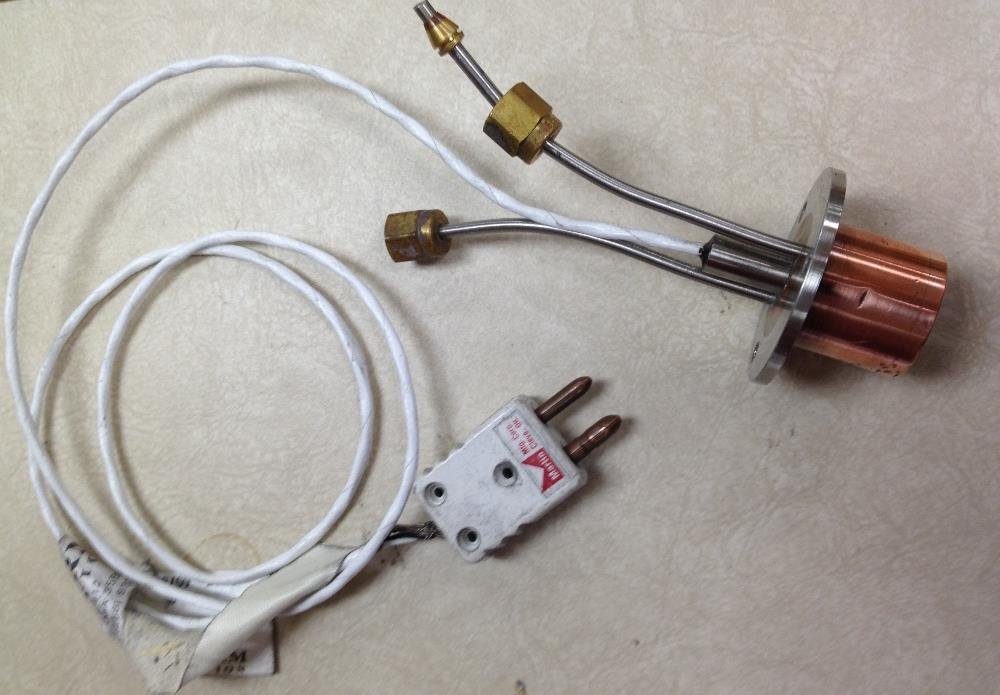
\includegraphics[width = 3.5in]{0_Images/Instrumentation/Heat_Flux_Gauge.jpg}
	\caption{Water Cooled Schmidt-Boelter Heat Flux Gauge}
	\label{fig:HeatFluxGauge}
\end{figure}

Temperatures were recorded using a bare-bead, Chromel-Alumel (type K) thermocouple with a 0.5 mm nominal diameter (Figure \ref{fig:Thermocouple}). The uncertainty given by the manufacturer for the temperature measurements is ±2.2 $^{\circ}$C for temperatures below 293 $^{\circ}$C and ±0.75\% for higher temperatures \cite{TemperatureHandbook}. The thermocouple readings will be lower than the air temperature when the thermocouple is in the flame region, due to radiative losses to the surrounding cooler environment. When the thermocouples are farther from the flame region, the impact of radiation will result in temperature readings higher than the air temperature. Due to the effect of radiative heat transfer to the thermocouples, the expanded uncertainty is approximately ±15\%.

\begin{figure} [H]
	\centering
	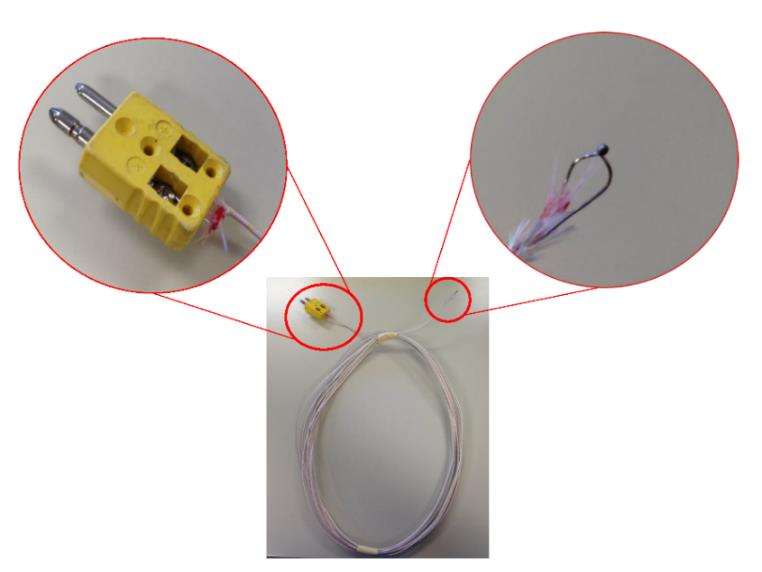
\includegraphics[width = 4in]{0_Images/Instrumentation/Thermocouple.jpg}
	\caption{Chromel-Alumel (Type K) Thermocouple}
	\label{fig:Thermocouple}
\end{figure}

Pressure was recorded through the use of a Setra Model 264 differential pressure transducer with a range of $\pm$0.5” WC ($\pm$124.5 Pa) (Figure \ref{fig:Setra}). The transducer was used to evaluate the pressure difference from ambient pressure. The uncertainty given by the manufacture is $\pm$\% or $\pm$1.2 Pa \cite{SetraManual}.

\begin{figure} [H]
	\centering
	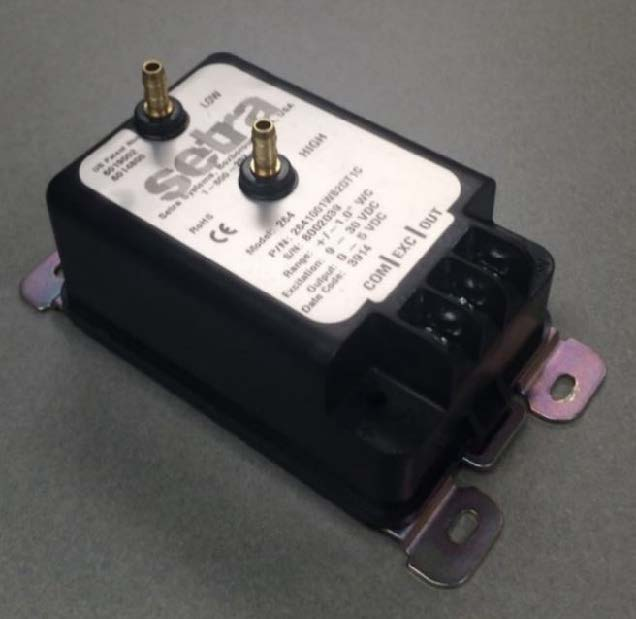
\includegraphics[width = 3in]{0_Images/Instrumentation/Setra.jpg}
	\caption{Setra Model 264 Differential Pressure Transducer}
	\label{fig:Setra}
\end{figure}

Gas velocity was obtained through the use of a bi-directional probe in conjunction with a differential pressure transducer and iconel thermocouple. The probe was constructed of stainless steel. The iconel thermocouple was a 0.063in. diameter type KSL iconel 600 sheathed grounded junction with a type K, 24 gauge glass/glass insulation lead. The differential pressure transducer was a Setra Model 264 with a range of $\pm$1.0in. WC ($\pm$248.8 Pa). The configuration had a velocity range of $\pm$24.2 m/s ($\pm$54 mph). The pressure transducers were configured in groups of 6, contained in a single plastic box with connections for pressure, temperature and power (Figure \ref{fig:BDP})b. Five probes were installed in openings where velocity measurements were taken, centered horizontally in the opening (Figure \ref{fig:BDP}a). Velocity measurement with this configuration was determined to have an uncertainty of $\pm$5\% \cite{BDPInPoolFires}.

\begin{figure} [H]
	\centering
	\begin{tabular}{c c}
		\subfloat[Pressure Transducer Box]{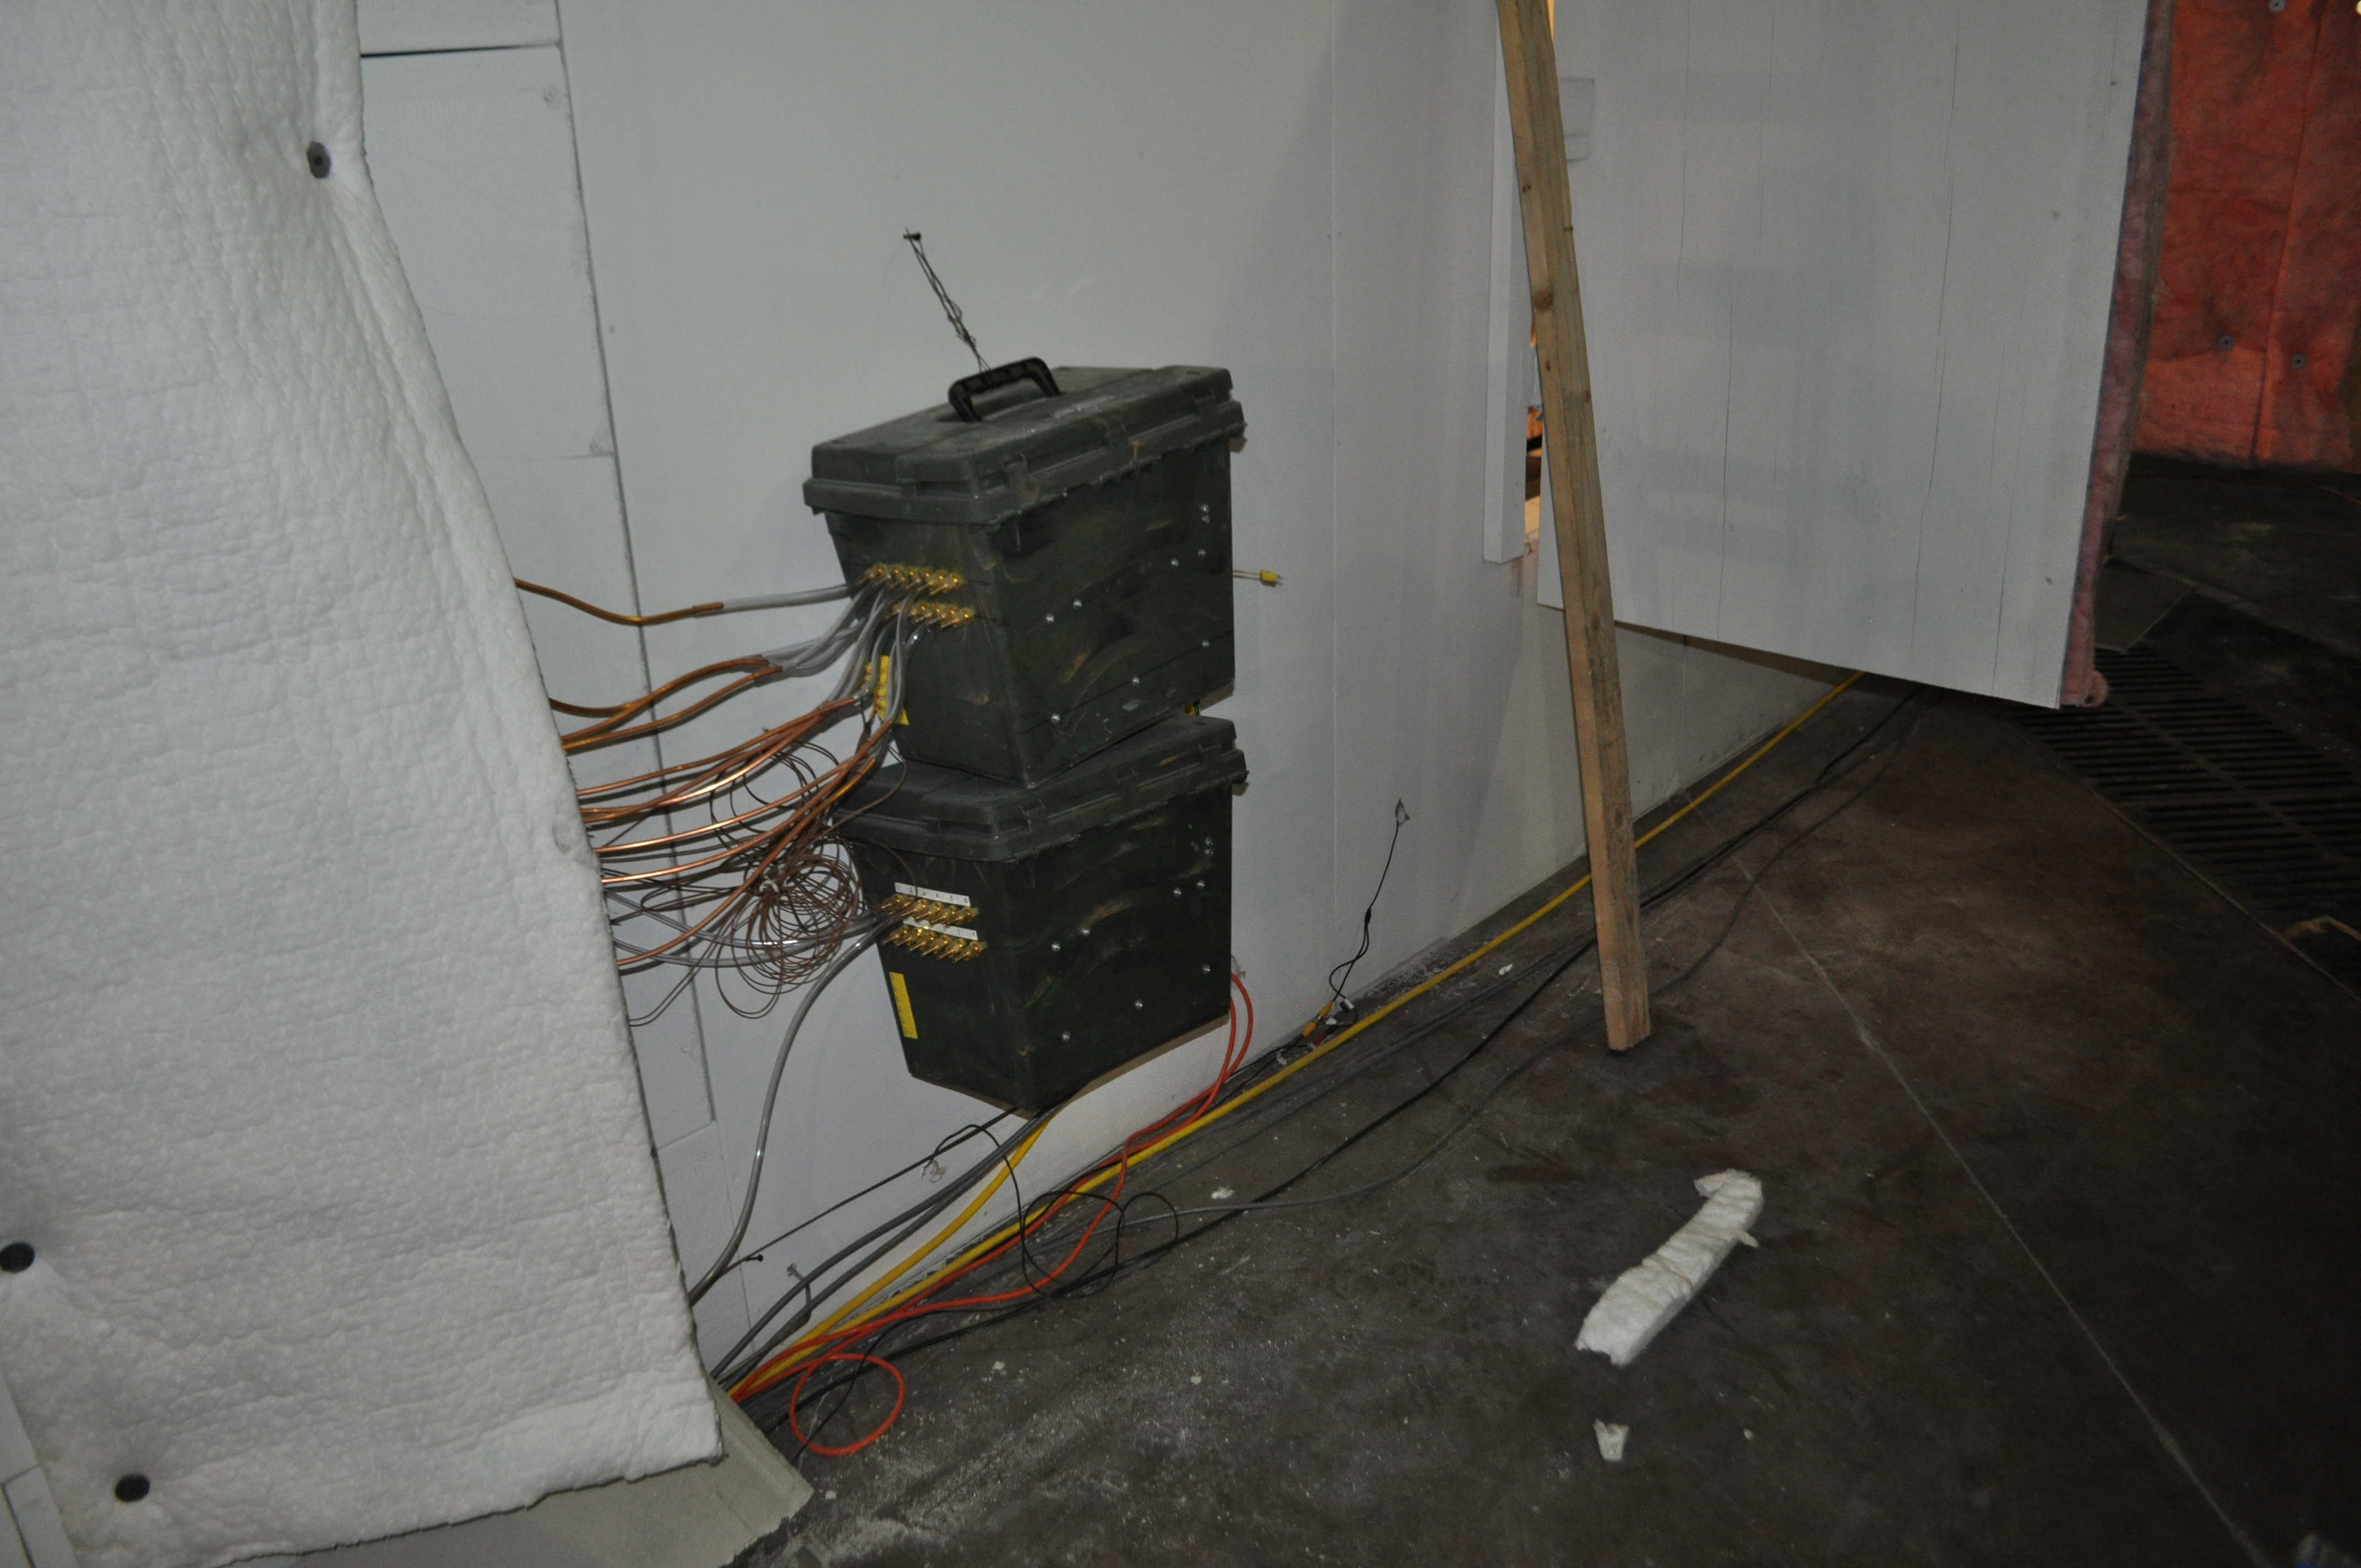
\includegraphics[height = 2.5in]{0_Images/Instrumentation/PressureBox.jpg}} &
		\subfloat[Bi-Directional Probe Array]{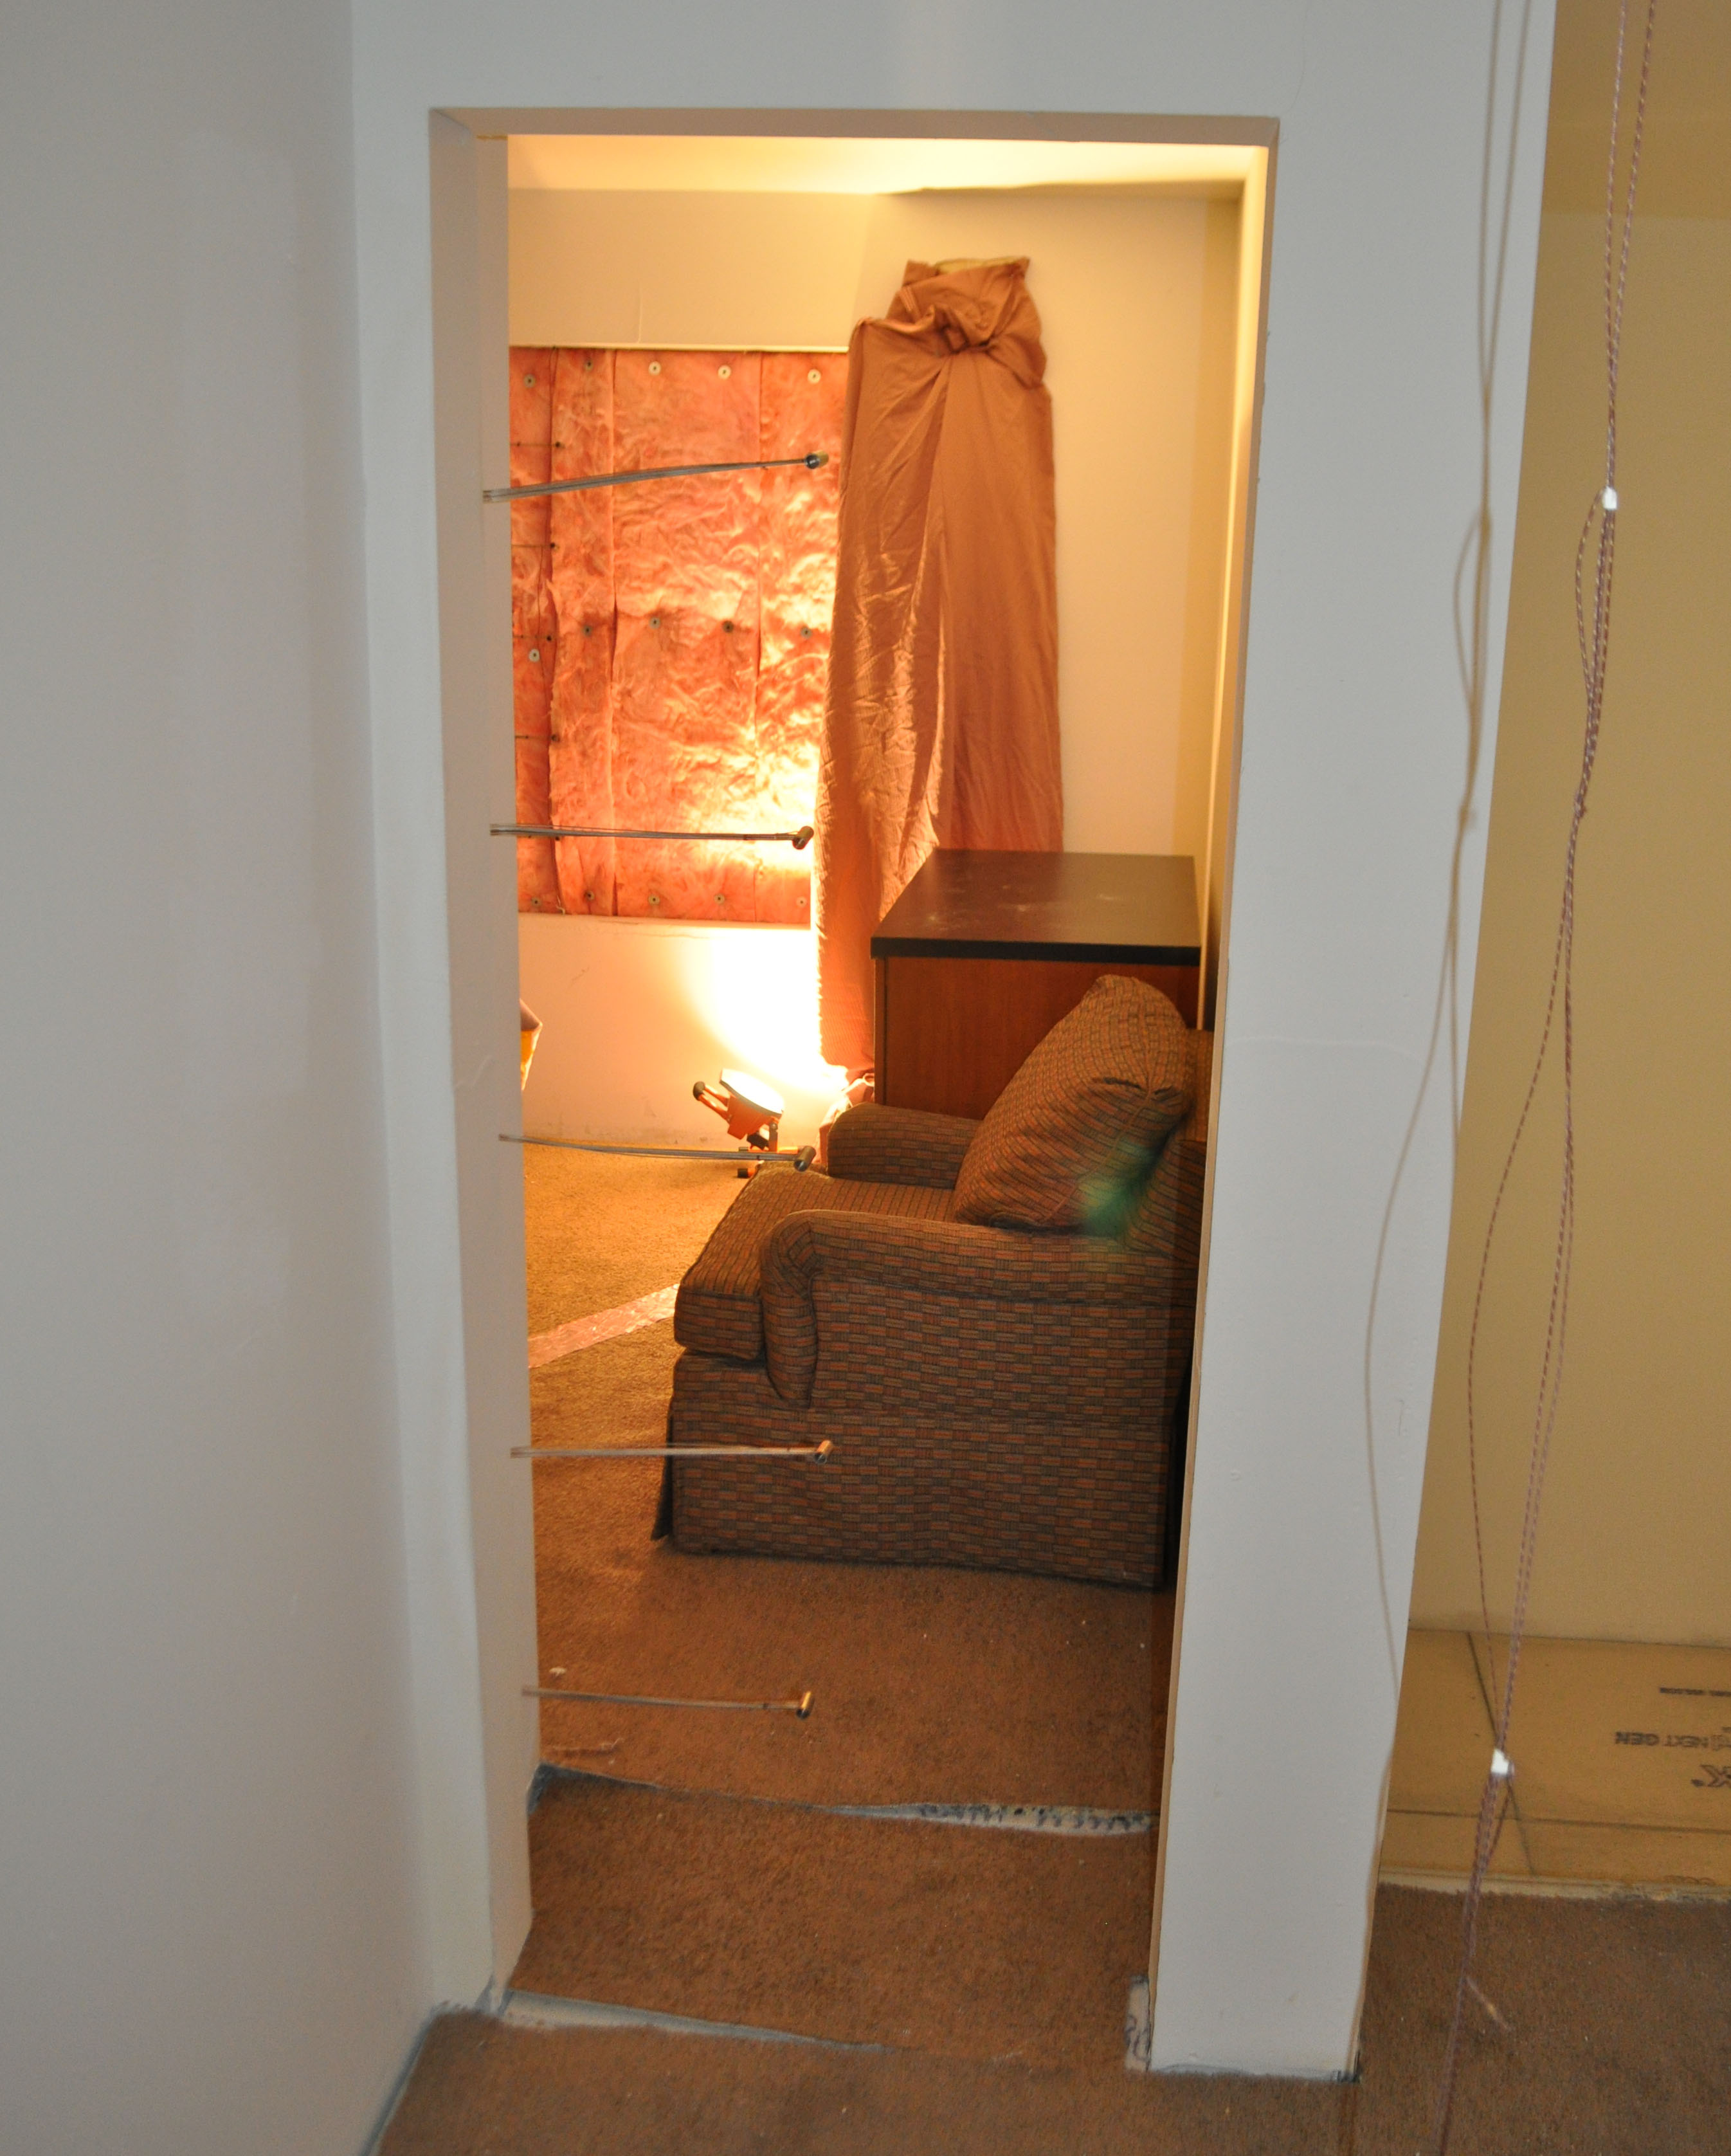
\includegraphics[height = 2.5in]{0_Images/Instrumentation/BDPArray.jpg}} \\
	\end{tabular}
	\caption{Bi-Directional Probe}
	\label{fig:BDP}
\end{figure}

The heat release rate is measured through the use of oxygen consumption techniques. The oxygen consumption calorimeter is capable of accurately measuring the heat release rate up to 10 MW. Above 10 MW, larger inaccuracies are expected due to the combustion products overflowing the collection hood. Figure \ref{fig:Hood} shows the collection hood utilized for the calorimetry data.

\begin{figure} [H]
	\centering
	\includegraphics[width = 5in]{0_Images/Instrumentation/Calorimetry_hood.jpg}
	\caption{Oxygen Consumption Calorimetry Hood}
	\label{fig:Hood}
\end{figure}

Stand video was obtained through the use of BoschVTC-206F03-4 video cameras (Figure \ref{fig:BullettCam}). Thermal imaging of the front and rear of the structure was taken using ISG Infrasys Elite XR (Figure \ref{fig:IRCam}). The thermal imaging camera has a fixed emissivity value of 0.9 and was utilized for visual representation of relative conditions, no temperature measurements or analysis were derived using the camera. All cameras were recorded using a TriCaster 8200 video acquisition system.

\begin{figure} [H]
	\centering
	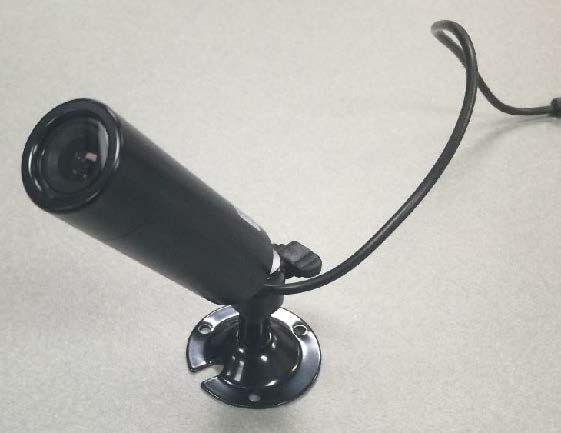
\includegraphics[width = 3in]{0_Images/Instrumentation/BullettCam.jpg}
	\caption{Bosch VTC-206F03-4 Video Camera}
	\label{fig:BullettCam}
\end{figure}

\begin{figure} [H]
	\centering
	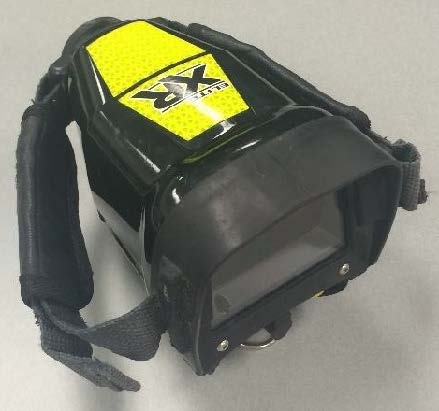
\includegraphics[width = 2.5in]{0_Images/Instrumentation/ISG_IR.jpg}
	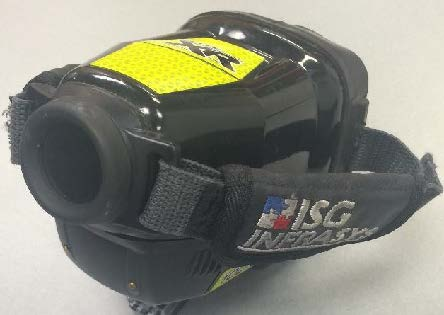
\includegraphics[width = 2.5in]{0_Images/Instrumentation/ISG_IR2.jpg}
	\caption{ISG Elite XR Fire Service Thermal Imaging Camera}
	\label{fig:IRCam}
\end{figure}

Gas samples were analyzed through the use of OxyMat6 and UltraMat23 Siemens gas analyzers. Samples were pulled from the structure through the use of cole palmer model L-79200-30 vacuum/pressure diaphragm pump rated at 0.75CFM via a stainless steel tube. The sample is filtered through a course filter, solberg model 842, 2 micron paper filter before running through a condensing trap to remove moisture. The sample then runs through a drying tube dry fine filter, perma pure model FF-250-SG-2.5G with a 1micron filter FF-250-E-2.5G before splitting into two branches and entering the UltraMat and OxyMat analyzer. The analyzers are calibrated to measure CO from 0-50000PPM, CO2 from 0-20\% and O$_2$ from 0-25\%. 

\begin{figure}[H]
	\centering
	\begin{tabular}{*3c}
		\subfloat[Sample Line]{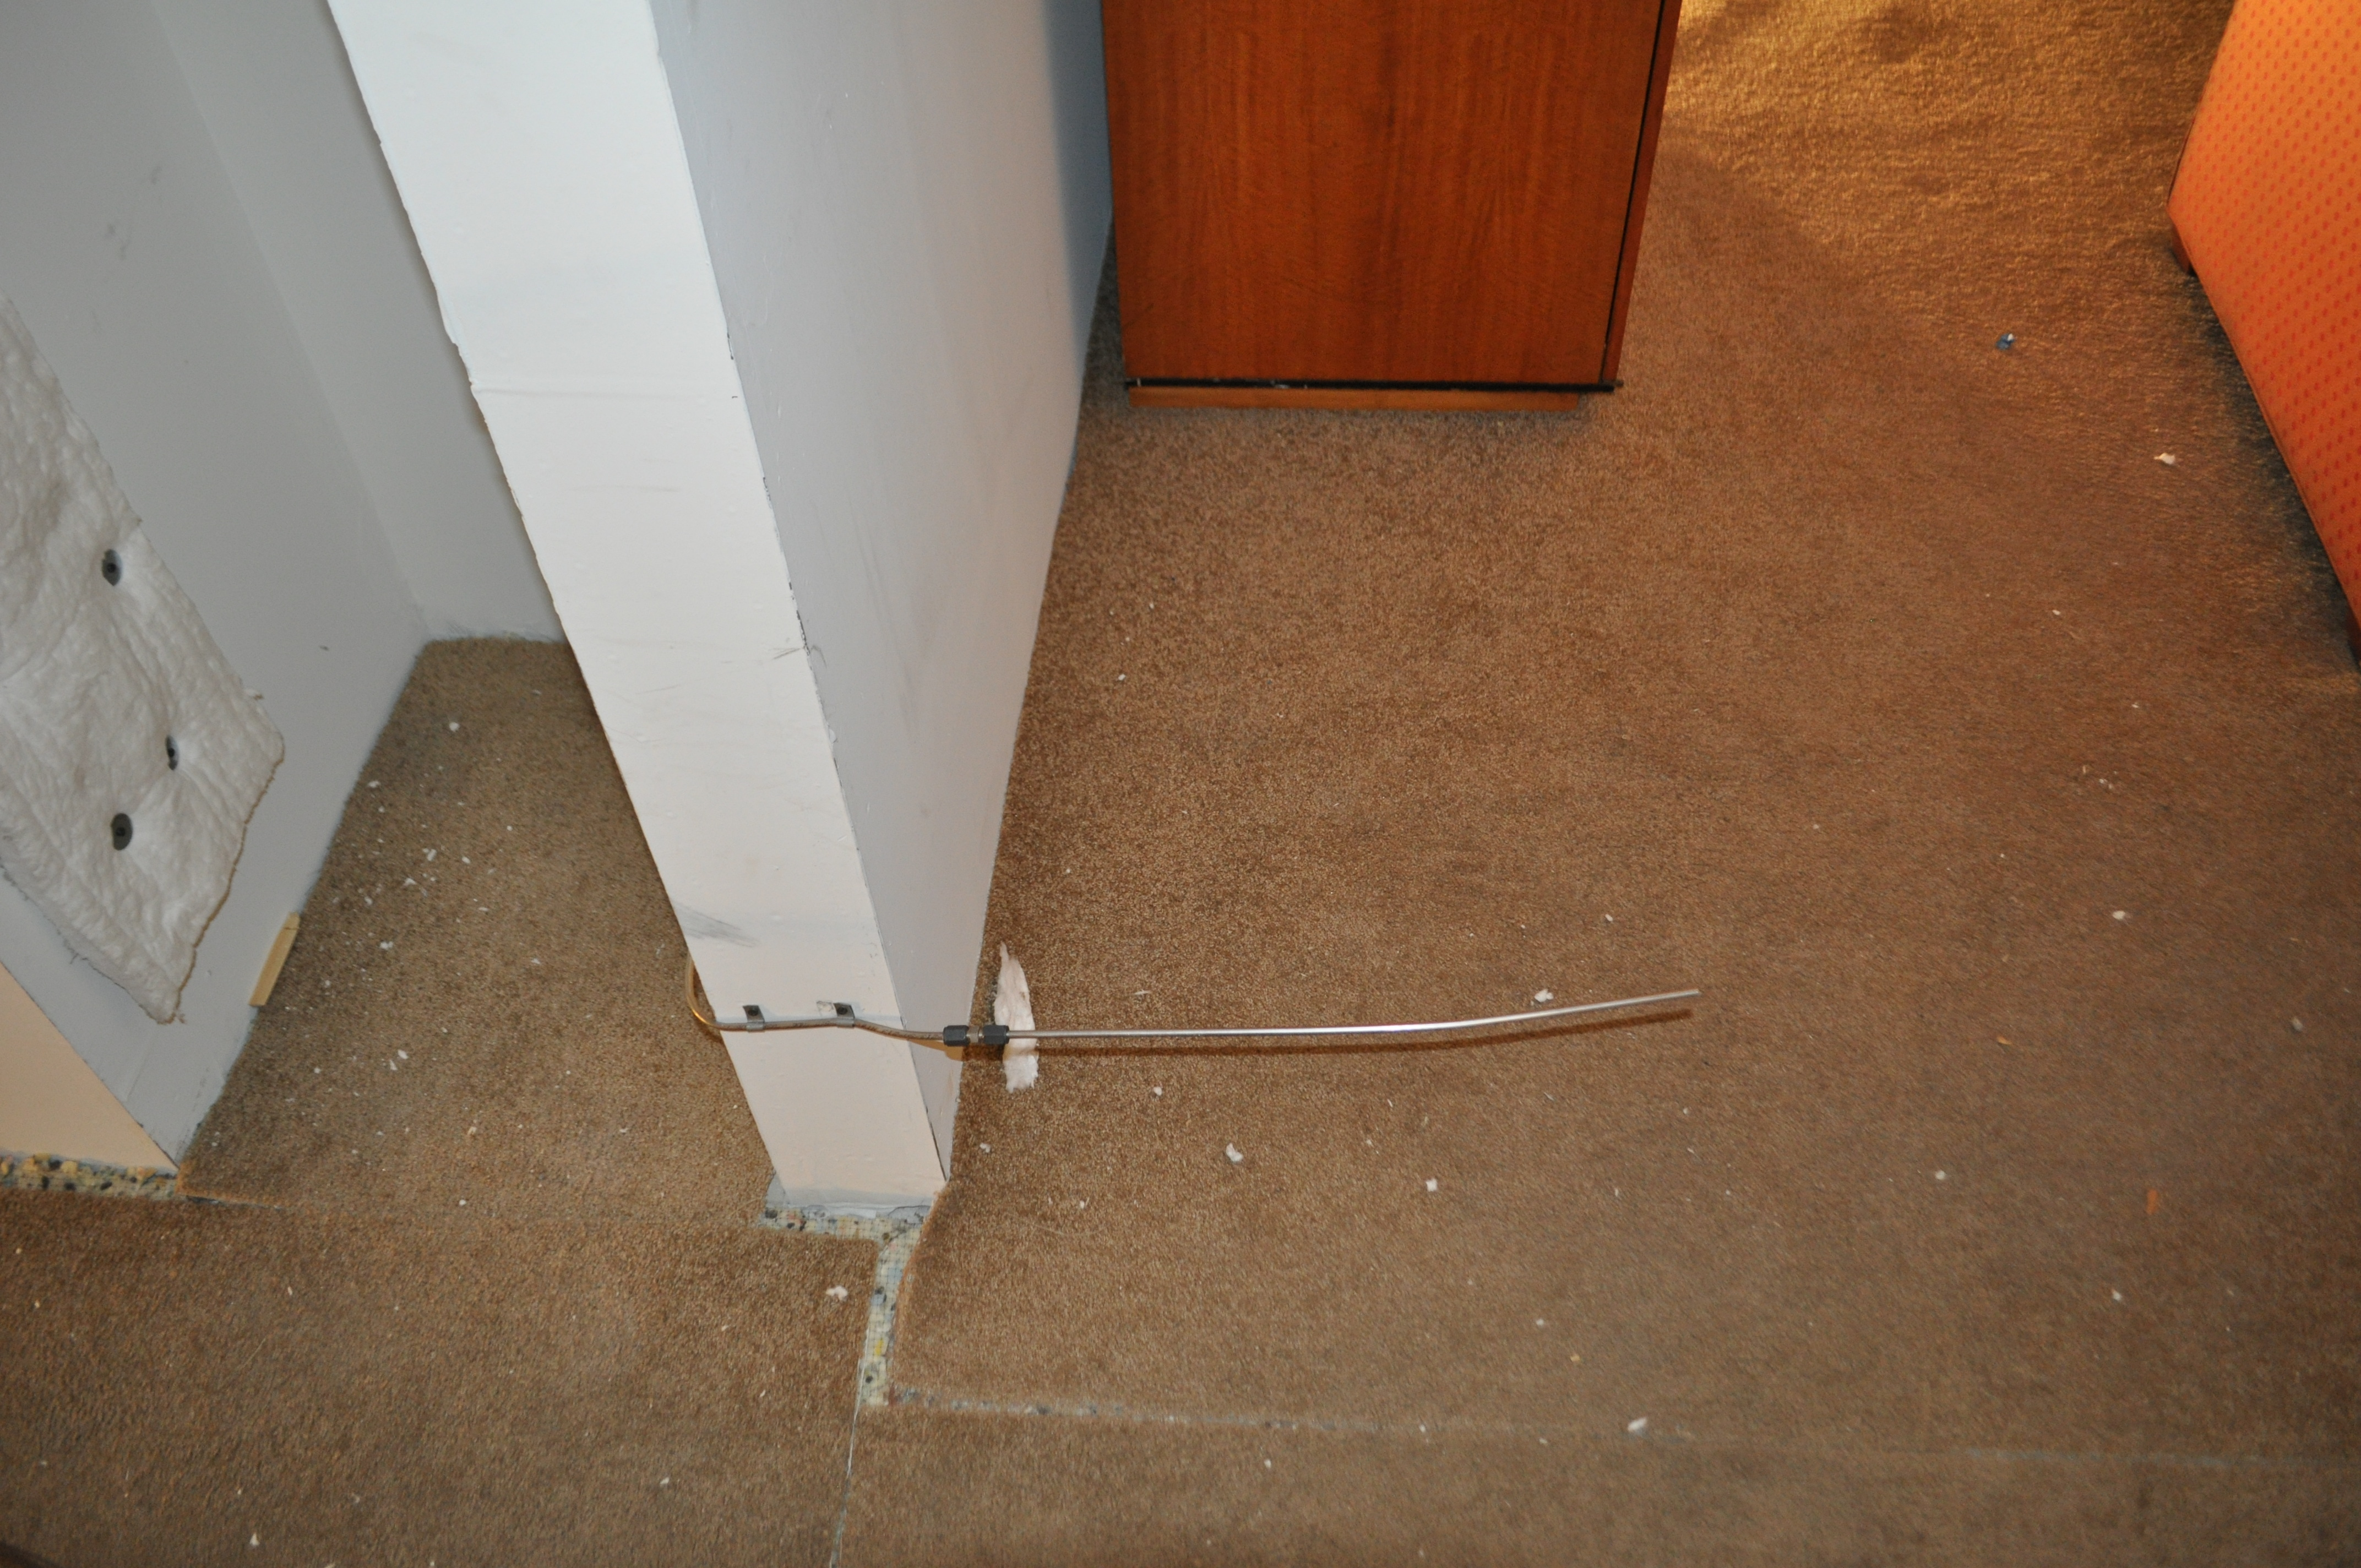
\includegraphics[width = 2in]{0_Images/Instrumentation/Gas_Analyzer/SamplePoint.jpg}} &
		\subfloat[Vaccum Pump - Cole Palmber L-79200-30]{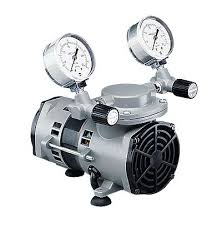
\includegraphics[width = 2in]{0_Images/Instrumentation/Gas_Analyzer/VaccumPump.jpg}} &
		\subfloat[Course Filter - Solberg 842]{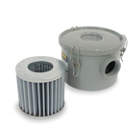
\includegraphics[width = 2in]{0_Images/Instrumentation/Gas_Analyzer/CourseFilter.jpg}} \\
		\subfloat[Condensing Tube]{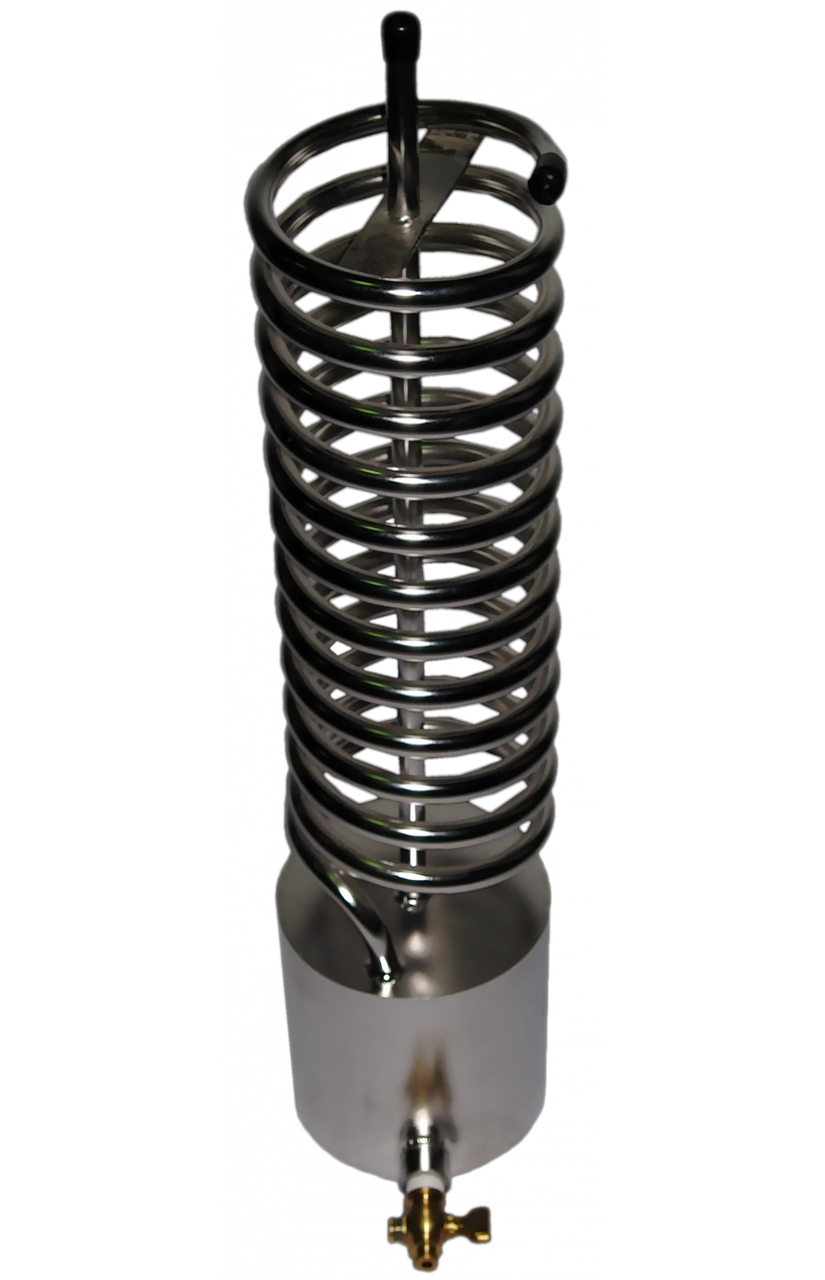
\includegraphics[height = 2in]{0_Images/Instrumentation/Gas_Analyzer/CoilCondenser.png}} &
		\subfloat[Dririte Tube]{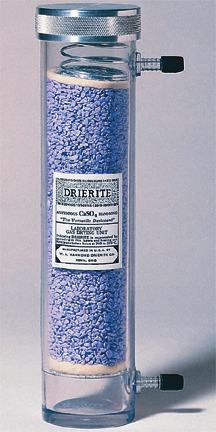
\includegraphics[height = 2in]{0_Images/Instrumentation/Gas_Analyzer/DriRightTube.jpg}} &
		\subfloat[Fine Filter - Perma Pure FF-250-SG-2.5G]{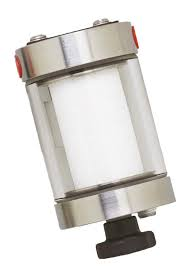
\includegraphics[height = 2in]{0_Images/Instrumentation/Gas_Analyzer/FineFilter.jpg}} \\
	\end{tabular}
	\subfloat[Gas Analyzers]{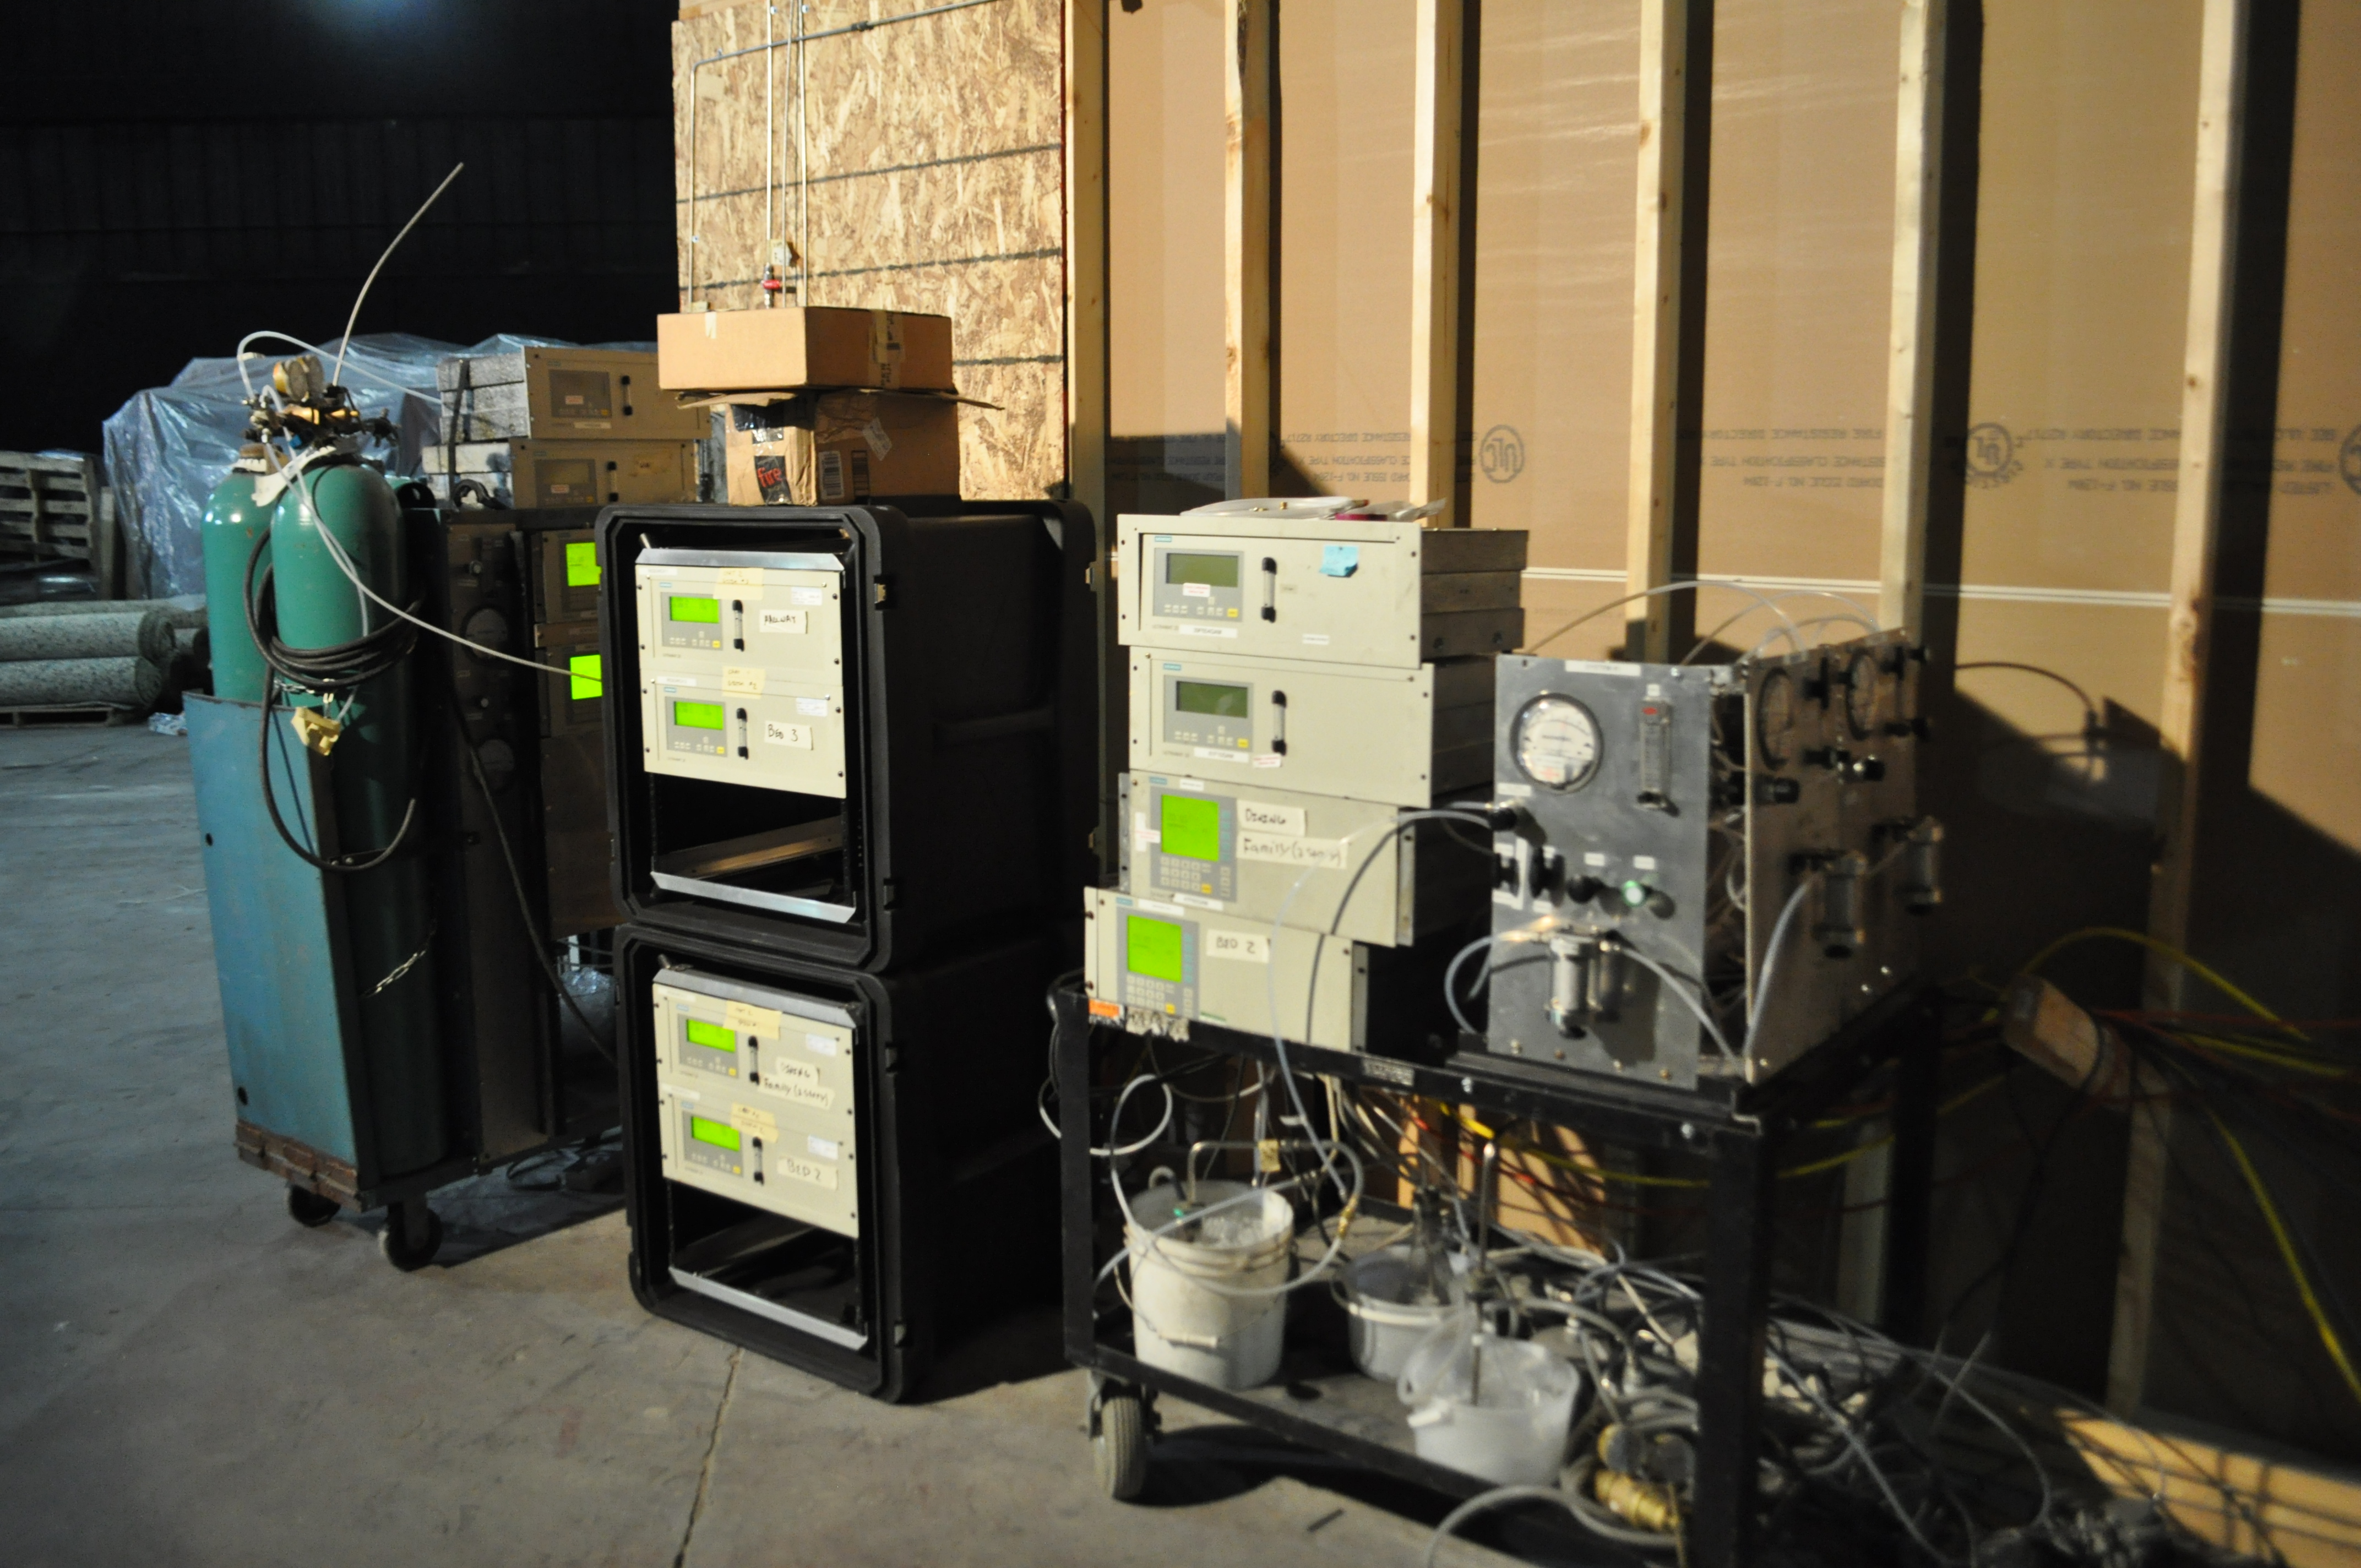
\includegraphics[width = 2in]{0_Images/Instrumentation/Gas_Analyzer/GasAnalyzers.jpg}}
	\caption{Gas Analyzer Configuration}
	\label{fig:GasAnalyzers}
\end{figure}

All data was logged through the use of a national instruments data acquisition system incorporating a SCXI-1001 chassis with 8 SCXI-1102C 32-Channel modules (Figure \ref{fig:DataSystem}). The system is configured for a total of 256 channels capable of reading values between 0-10 volts DC. Values are recorded once a second and translated to quantities of interest through the use of LabVIEW software specifically programmed for use with the system.

\begin{figure}[H]
	\centering
	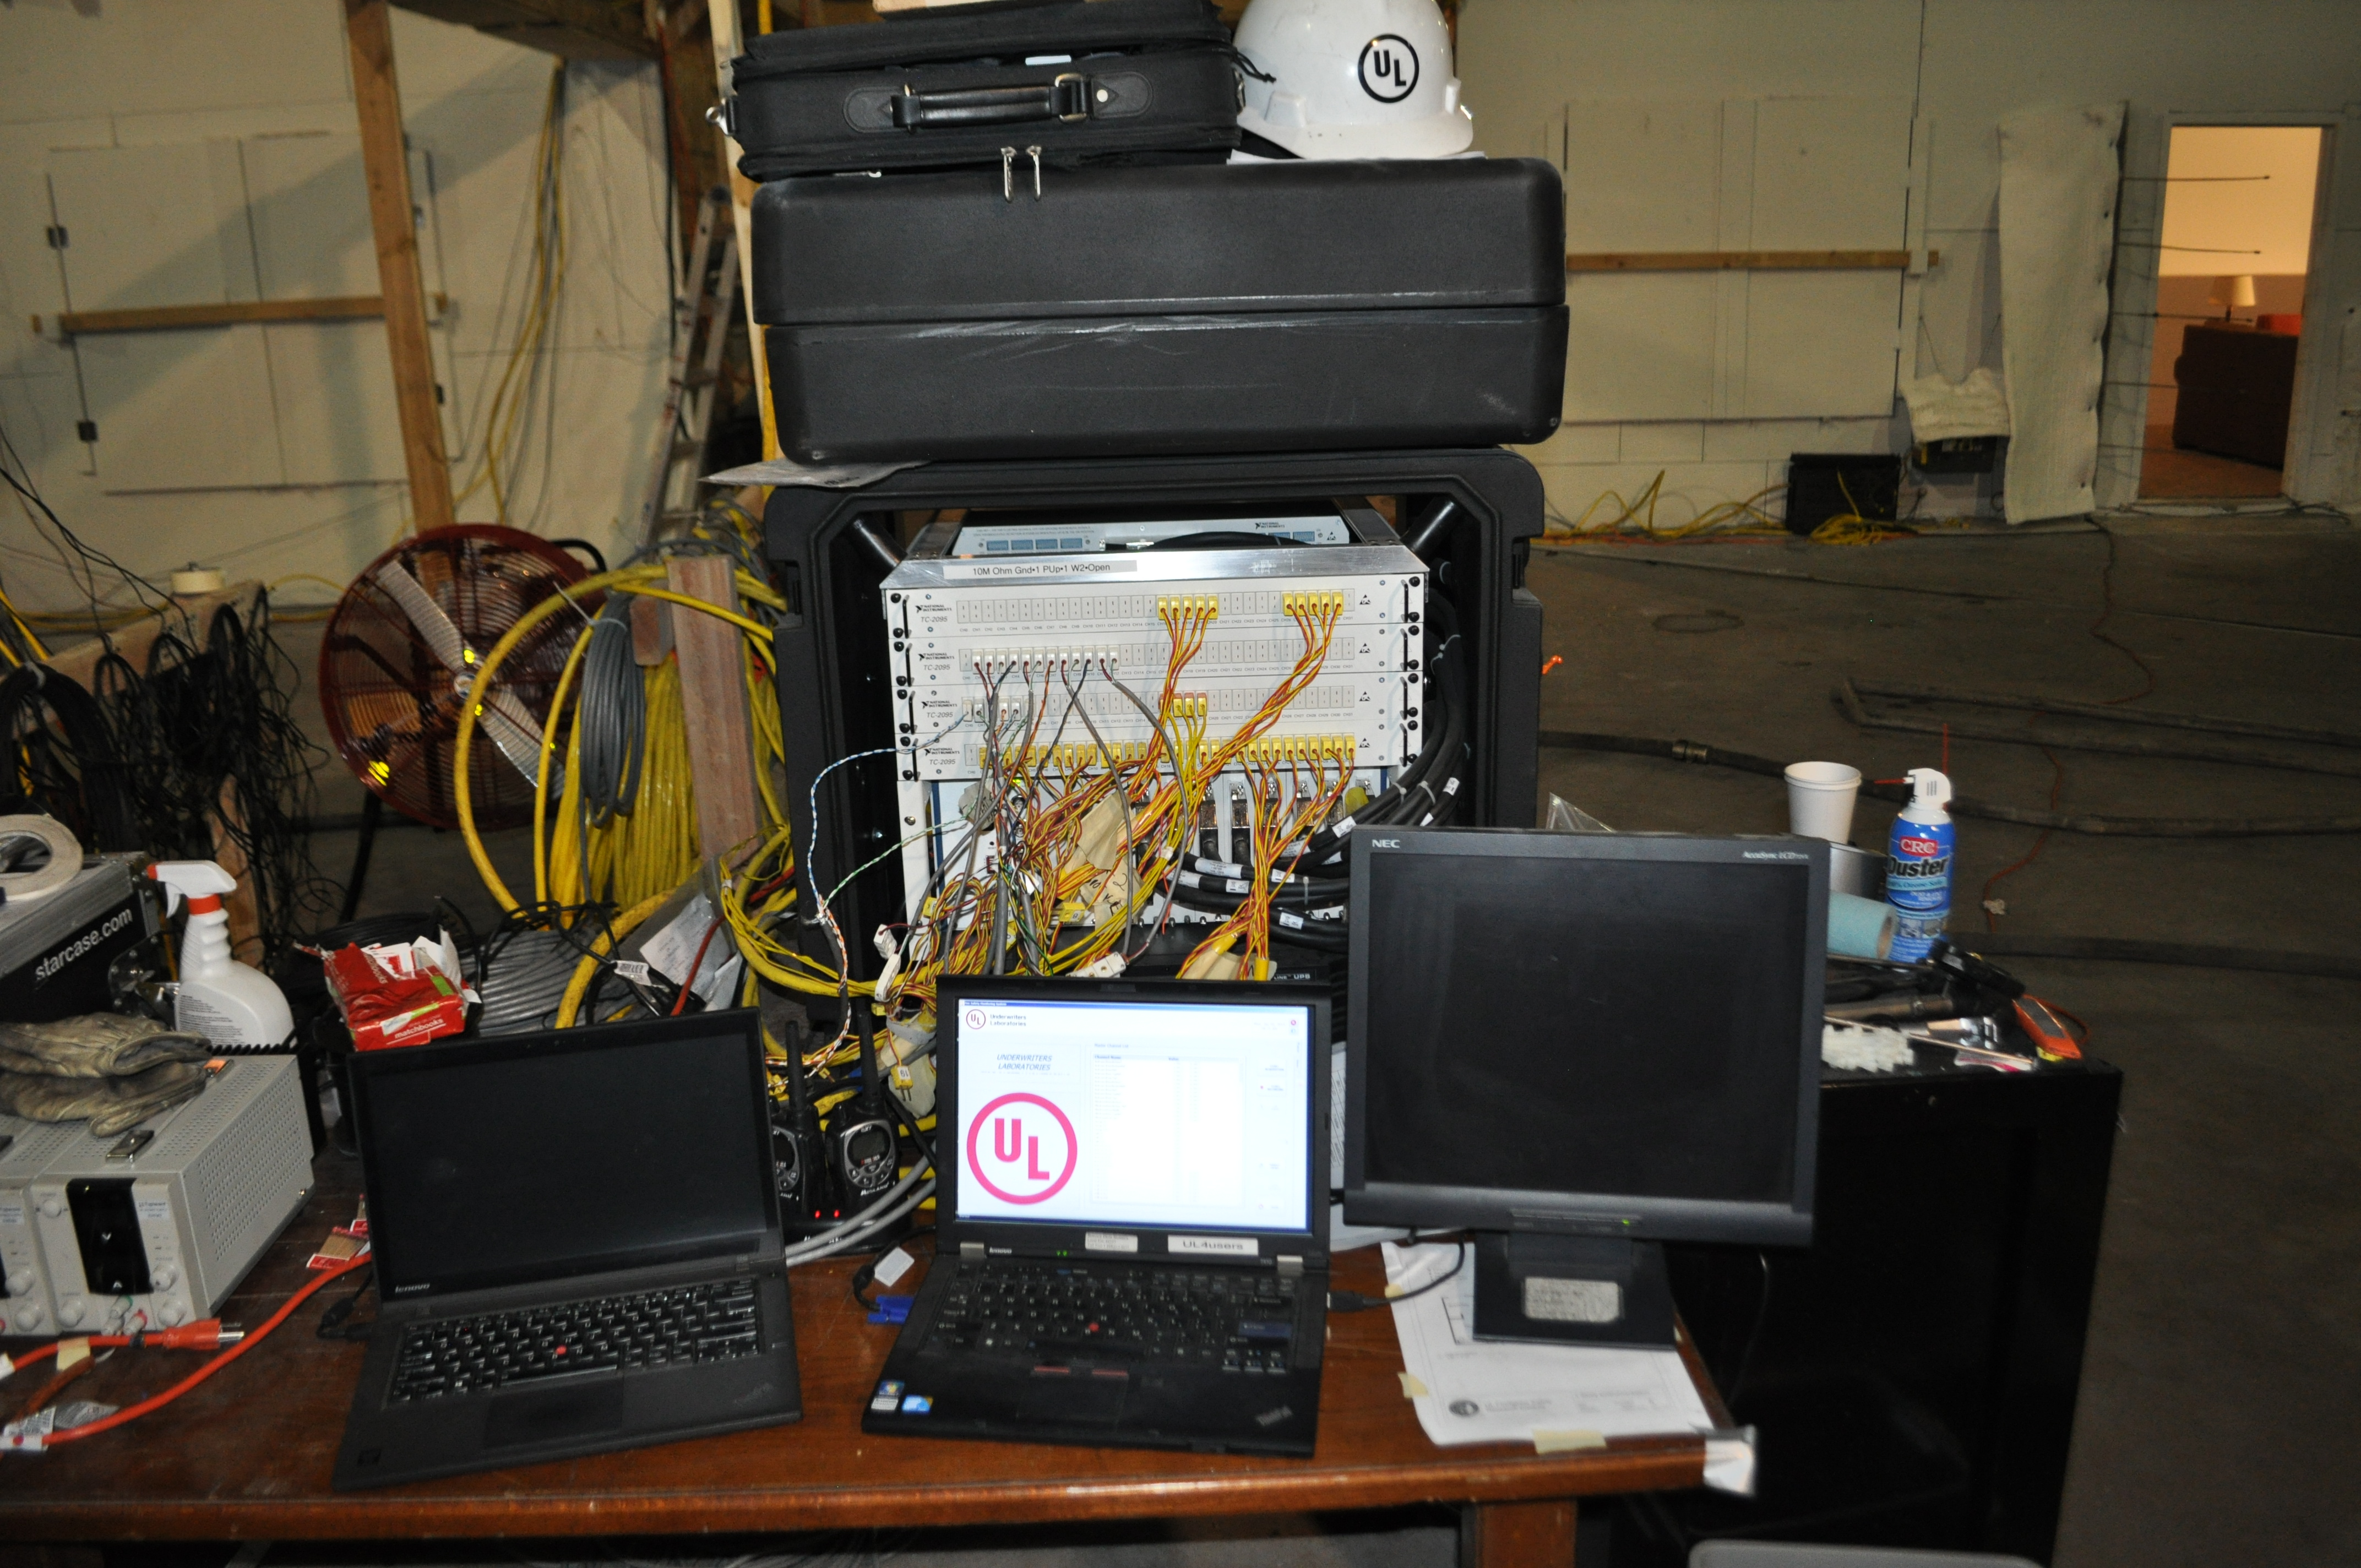
\includegraphics[width = 4in]{0_Images/Instrumentation/DataSystem.jpg}
	\caption{Data Acquisition System}
	\label{fig:DataSystem}
\end{figure}

\clearpage

\section{Test Set Up}

\subsection{Structures}

\paragraph{Single Story Structure} \mbox{}

The house was designed by a residential architectural company to be representative of a home constructed in the mid-twentieth century with walls and doorways separating all of the rooms and 8 ft. ceilings. The experiments aim to examine the fire dynamics in a structure of this type and to further understand the impact of positive pressure attack on tenability throughout the structure.

The one-story house had an area of 1200 $ft^2$, with 3 bedrooms, 1 bathroom and 8 total rooms (Figure \ref{fig:SingleStory}). The home was a wood frame, type 5 structure lined with two layers of gypsum board (Base layer 5/8 in, Surface layer 1/2 in.) The intent of the study was to focus on content fires thus no roof structure was included in the design. The ceilings were supported with engineered i-joists instead of engineered trusses. The front and rear of the structure were covered with cement board to limit exterior fire spread. Figure \ref{fig:SingleStoryISO} is a 3D rendering of the house with the roof cut away to show the interior layout with furniture and floor coverings. The tan floor shows the carpet placement and the grey show the cement floor or simulated tile locations. Construction plans can be found in appendix \ref{App:ConstructionDrawings}.

\begin{figure}[H]
	\centering
	\begin{tabular}{*2c}
		\subfloat[Single Story Side A]{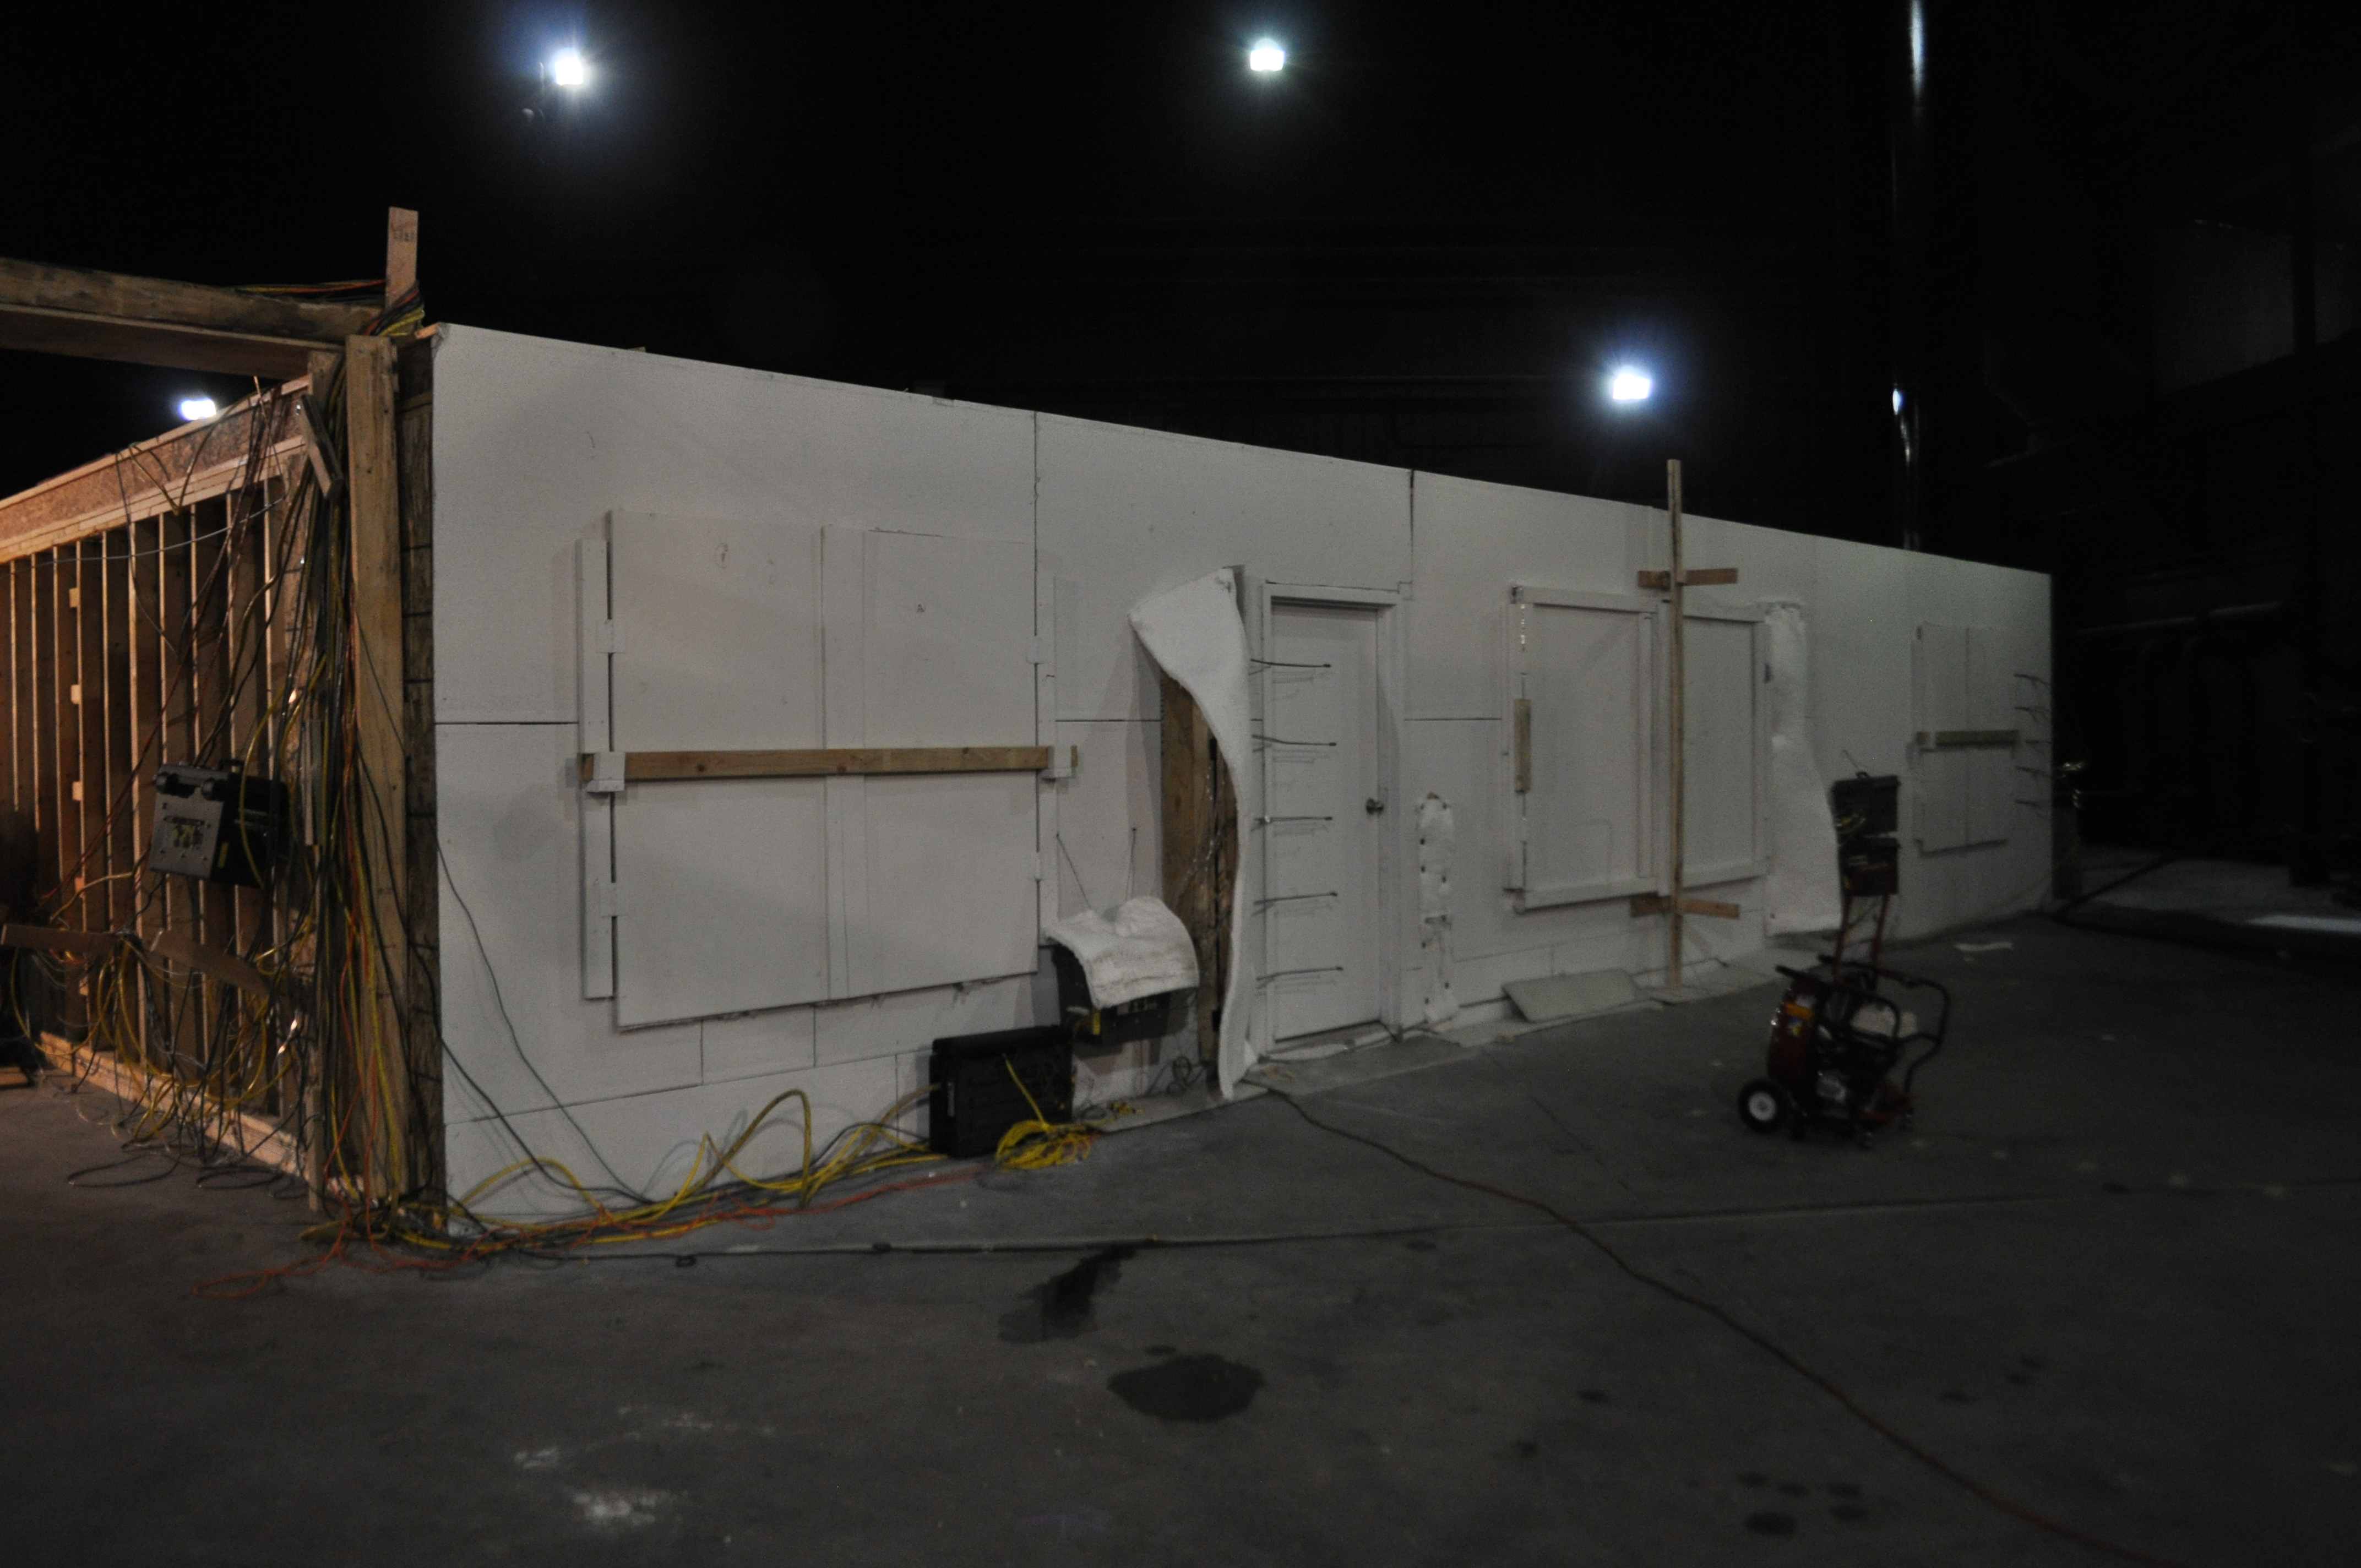
\includegraphics[width = 3in]{0_Images/Structures/SingleStory/ExteriorAB_Corner.jpg}} & 
		\subfloat[Single Story Side C]{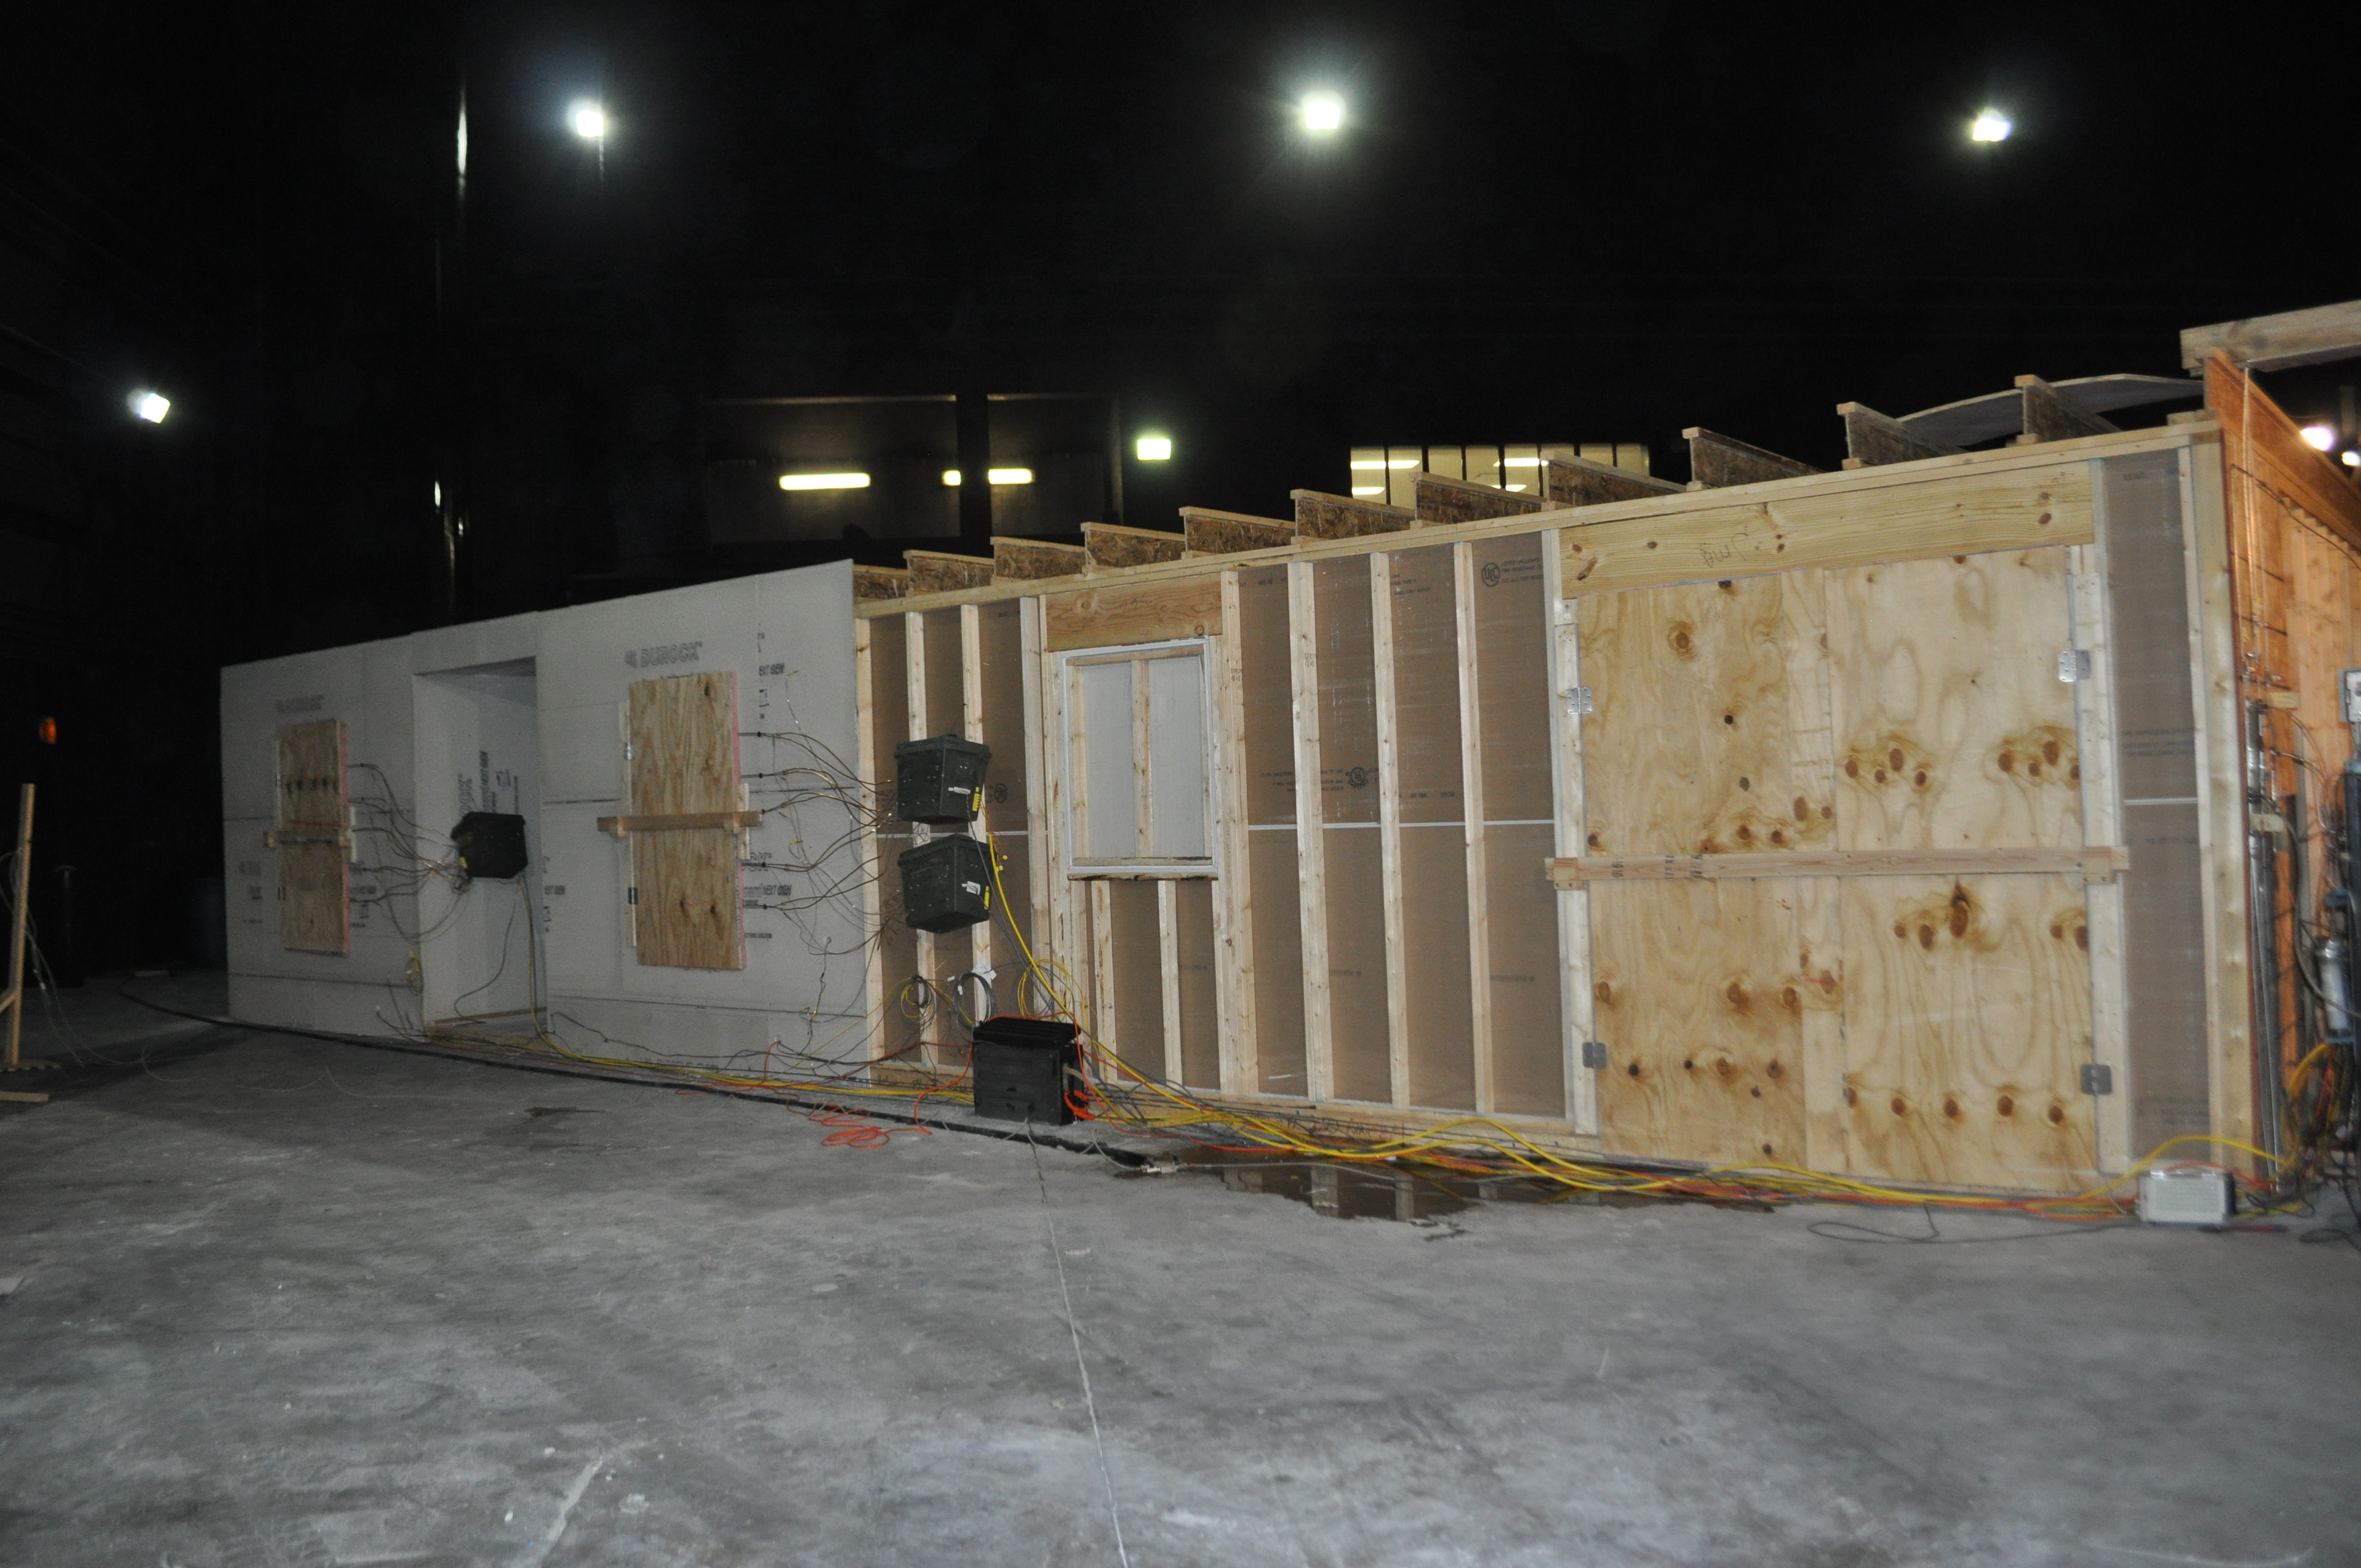
\includegraphics[width = 3in]{0_Images/Structures/SingleStory/ExteriorBC_Corner.jpg}} \\
	\end{tabular}
	\caption{Single Story Test Structure}
	\label{fig:SingleStory}
\end{figure}

\begin{figure}[H]
	\centering
	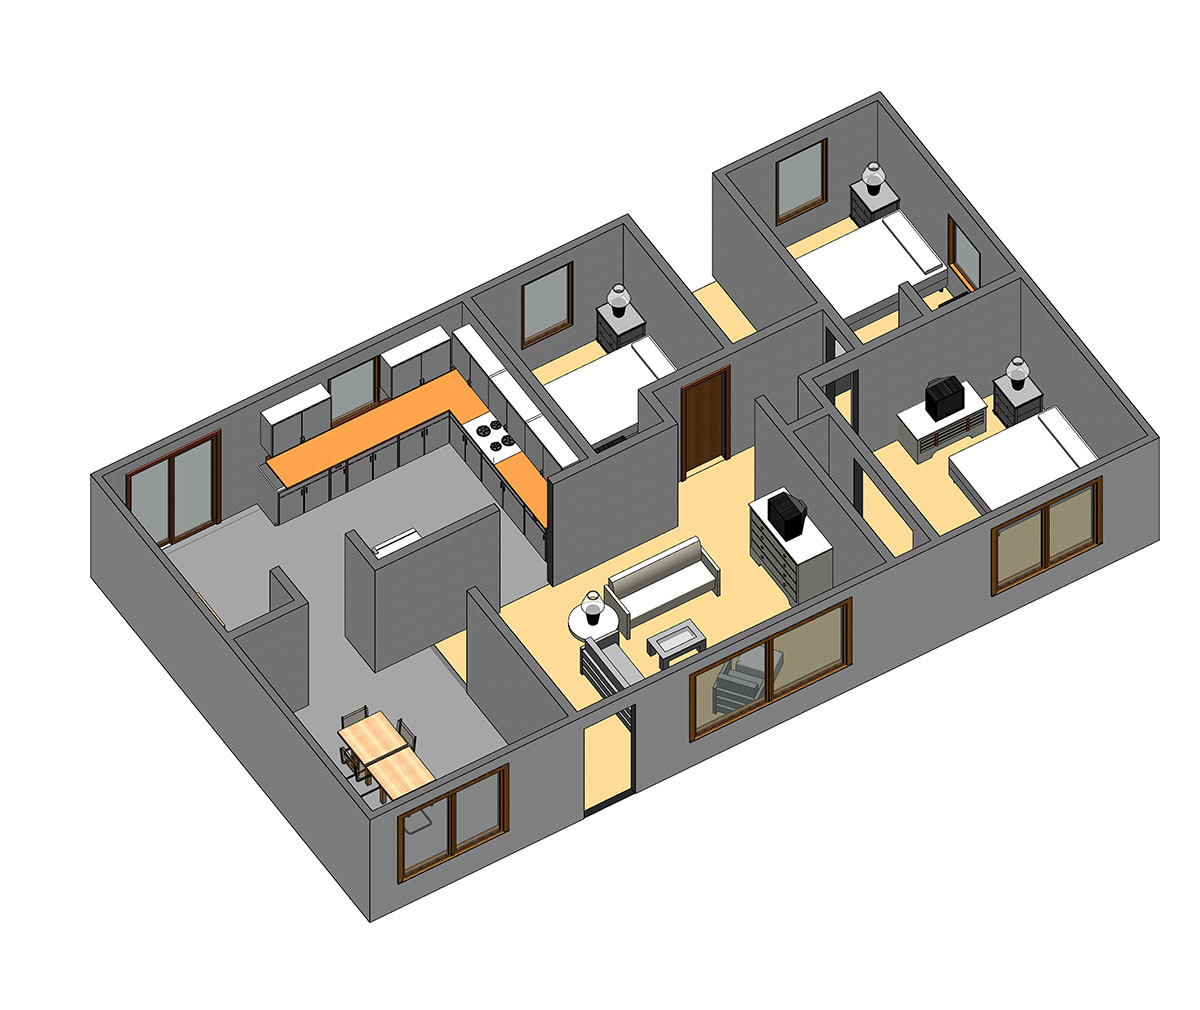
\includegraphics[width = 4in]{0_Images/Experiment_ISO/Single_Story_Base_Bed3_Closed.jpg}
	\caption{Single Story Isometric}
	\label{fig:SingleStoryISO}
\end{figure}

\paragraph{Two Story Structure} \mbox{}

The house was designed by a residential architectural company to be representative of a home constructed in the late-twentieth  early twenty-first century with an open floor plan, two story foyer and two story great room. The experiments aim to examine the fire dynamics in a structure of this type and to further understand the impact of positive pressure attack on tenability throughout the structure.

The two-story house had an area of 3200 $ft^2$, with 4 bedrooms, 2.5 bathrooms house and 12 total rooms (Figure \ref{fig:TwoStory}). This home was also a wood frame, type 5 structure lined with two layers of gypsum board (Base layer 5/8 in, Surface layer 1/2 in.) The intent of the study was to focus on content fires thus no roof structure was included in the design. The second floor ceilings were supported with engineered i-joists instead of engineered trusses. The front and rear of the structure were covered with cement board to limit exterior fire spread. Figure \ref{fig:TwoStoryISO} is a 3D rendering of the house with the roof cut away to show the interior layout with furniture and floor coverings. The tan floor shows the carpet placement and the grey show the cement floor or simulated tile locations. Construction plans can be found in appendix \ref{App:ConstructionDrawings}.

\begin{figure}[H]
	\centering
	\begin{tabular}{*2c}
		\subfloat[Two Story Side A]{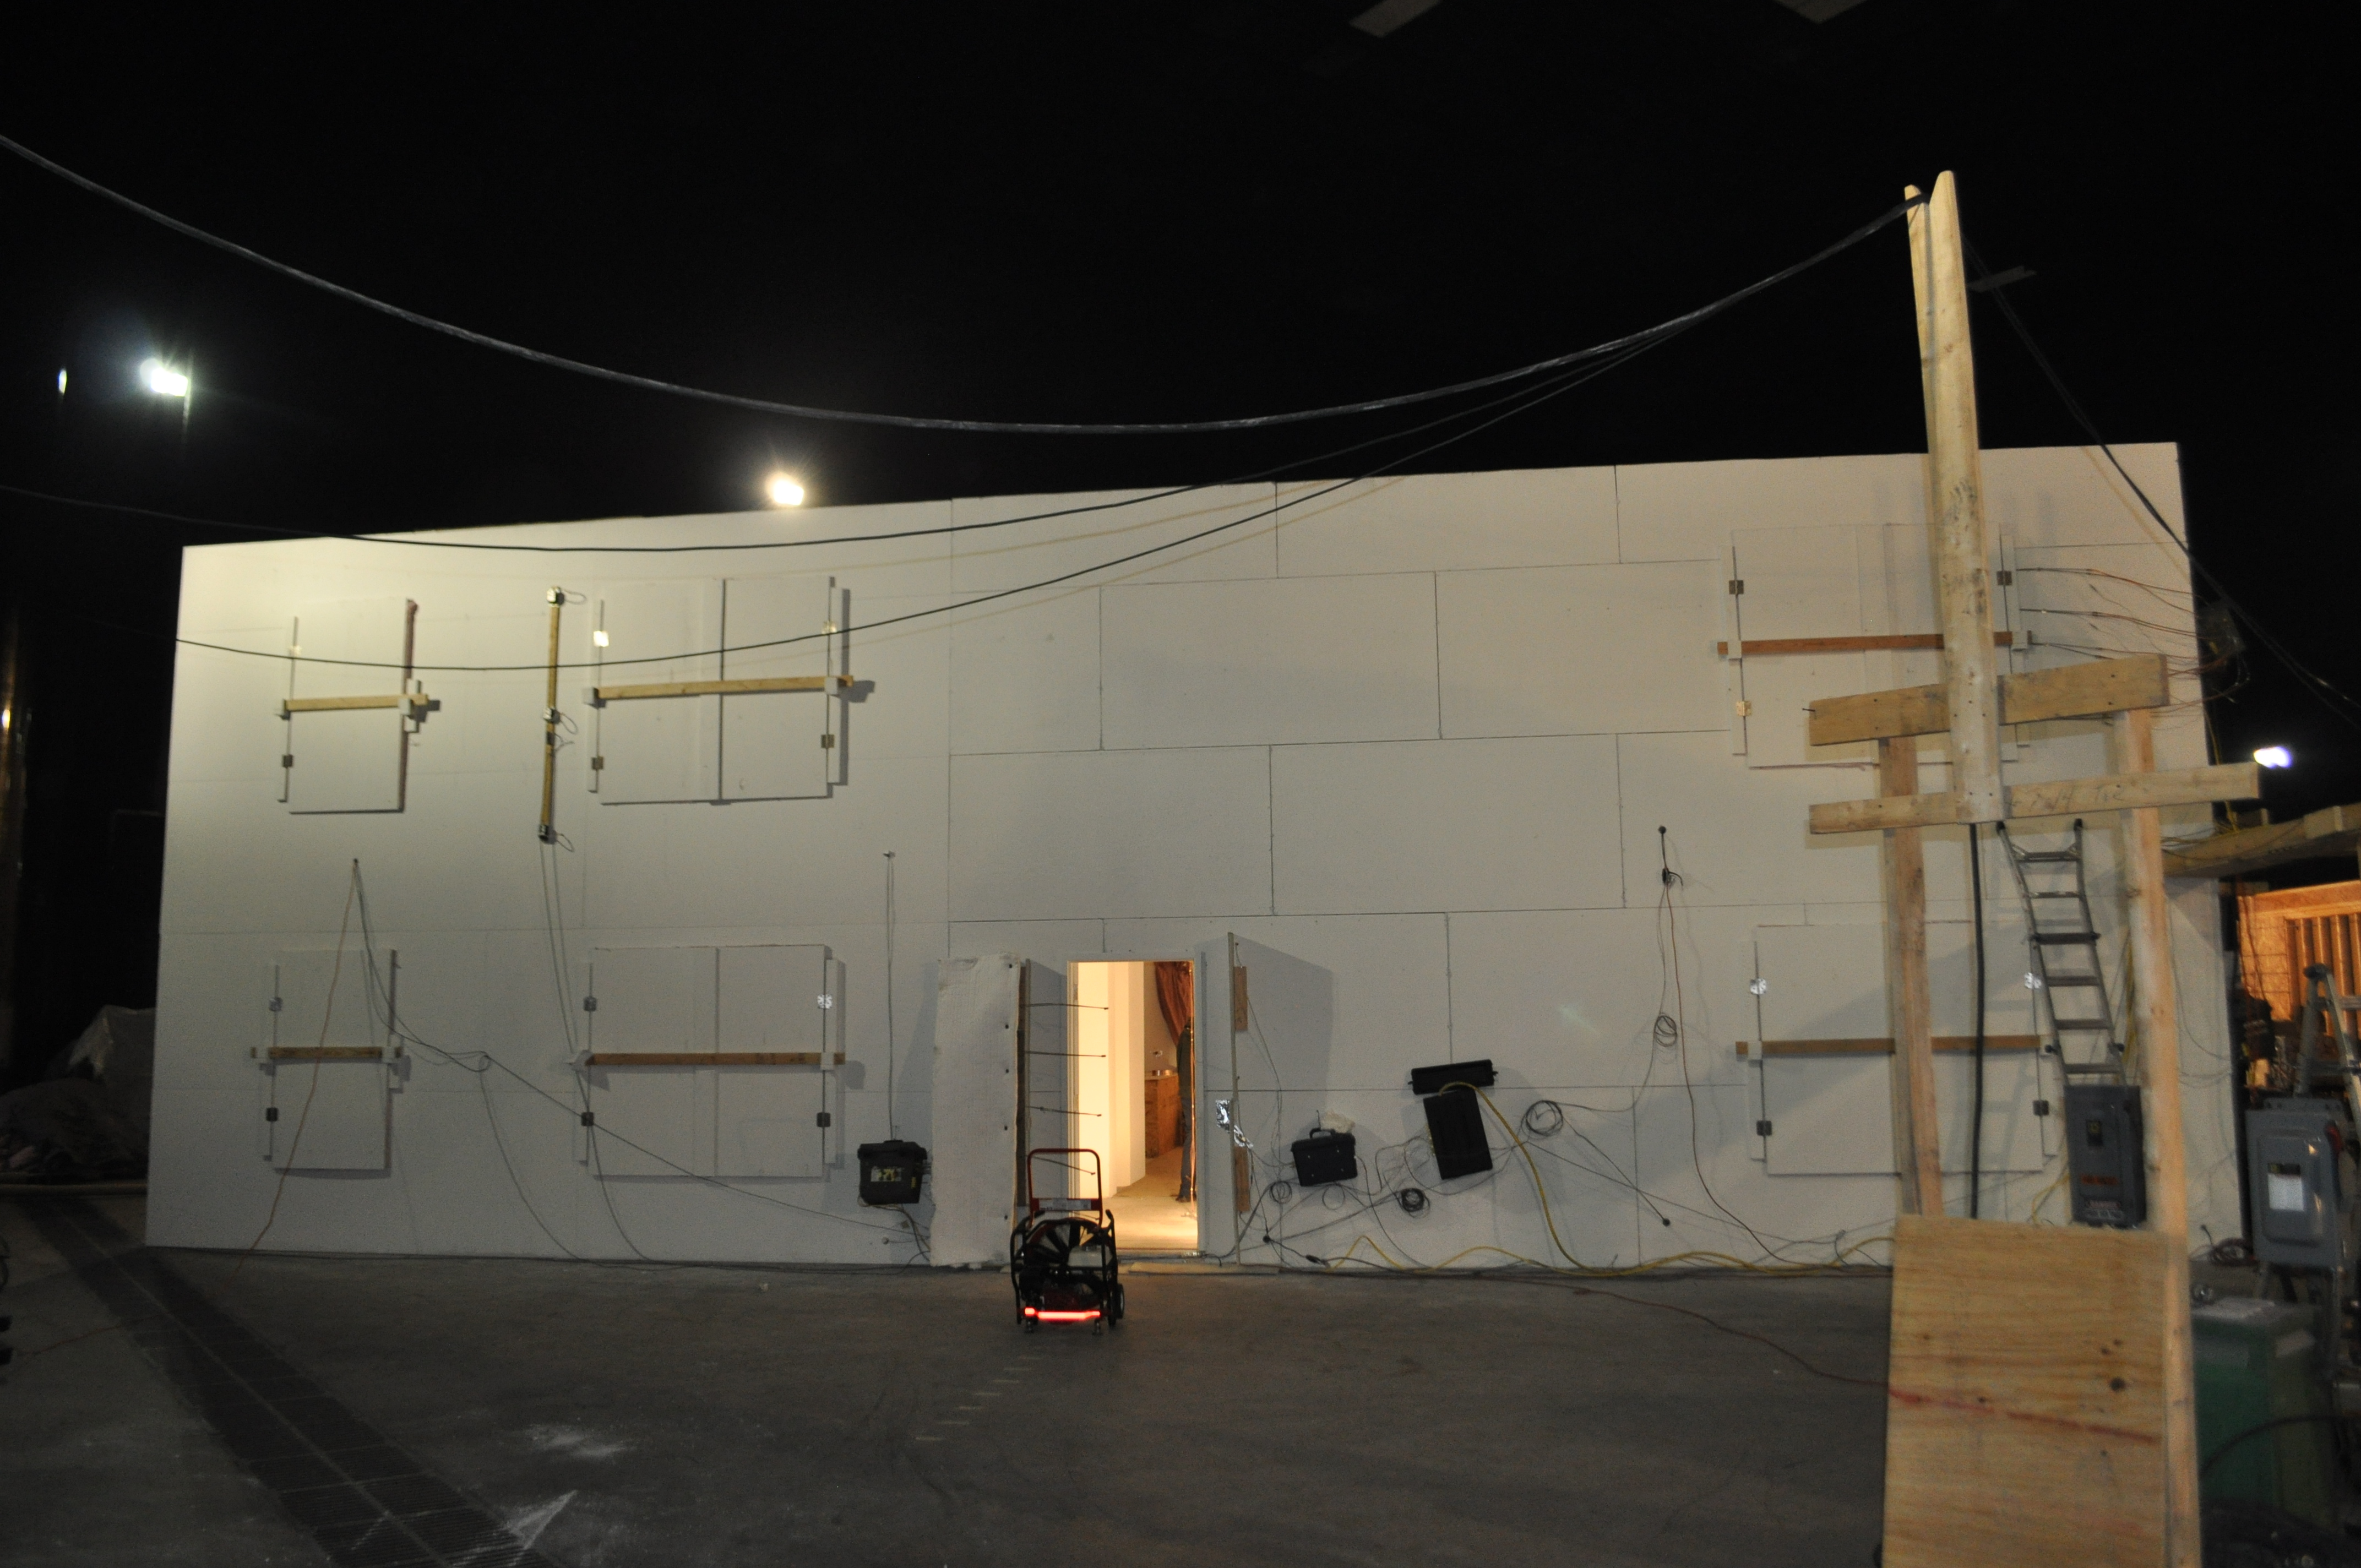
\includegraphics[width = 3in]{0_Images/Structures/TwoStory/ExteriorTwoStory_A.jpg}} & 
		\subfloat[Two Story Side C]{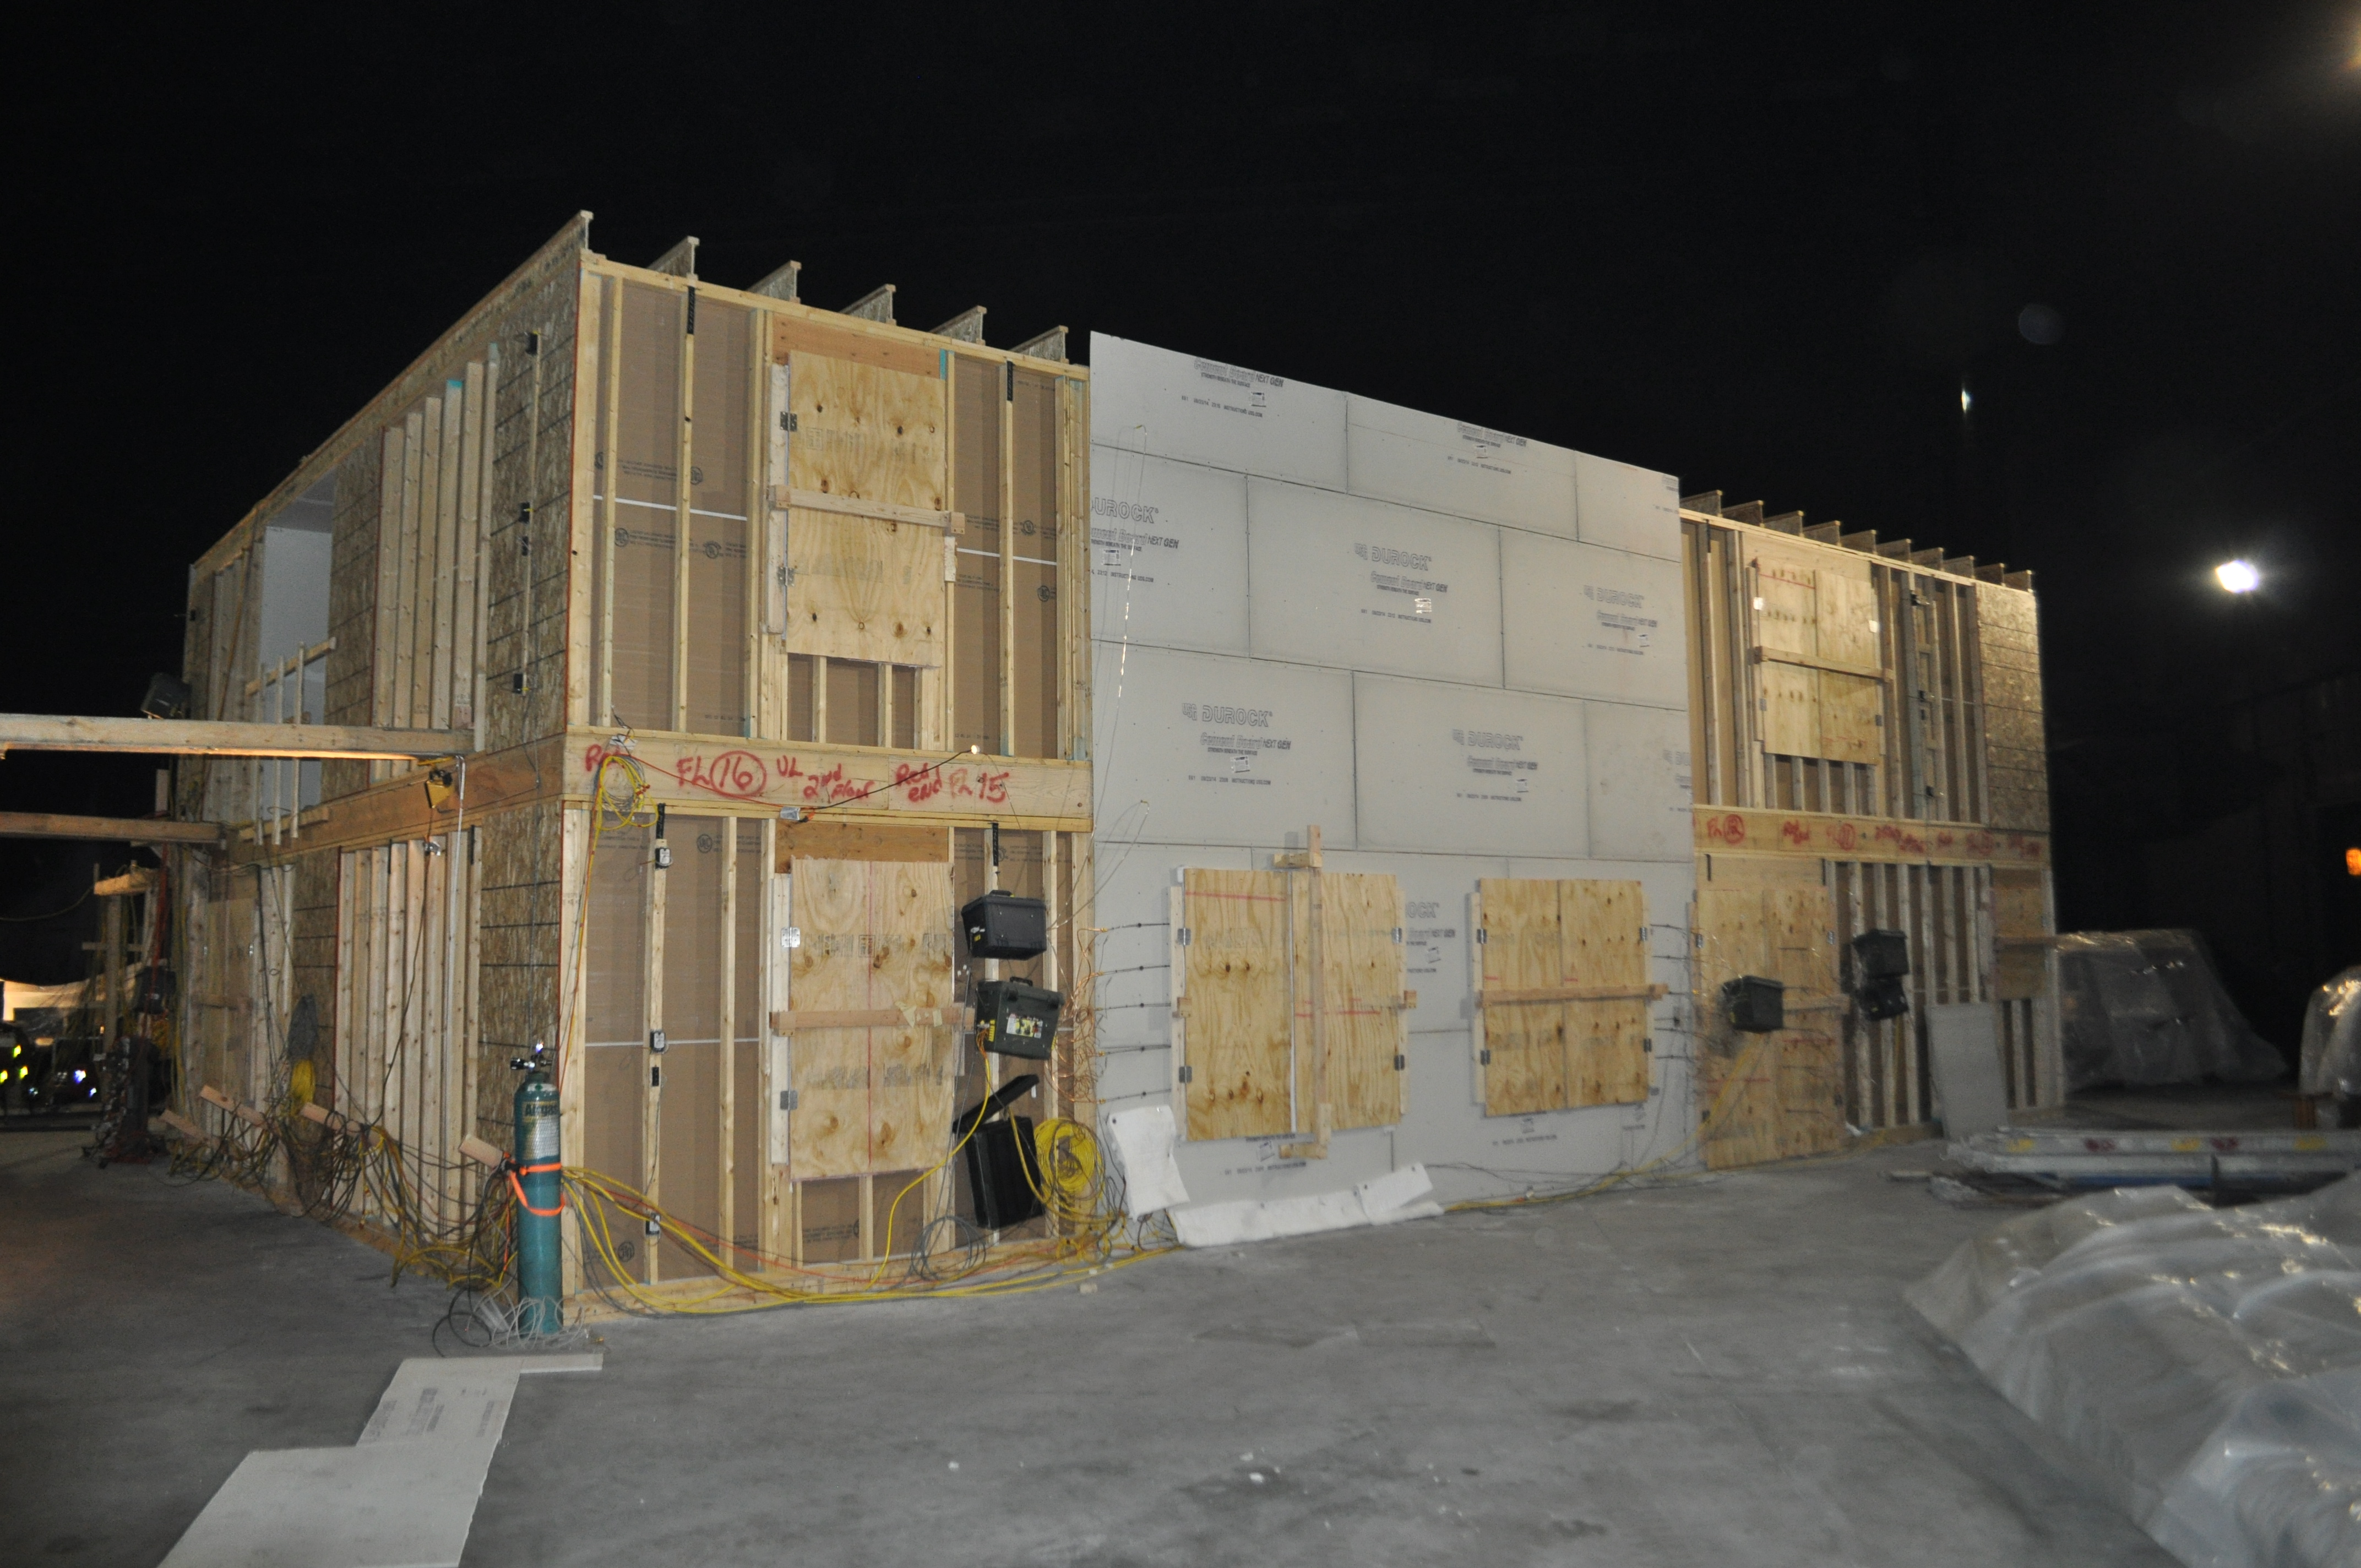
\includegraphics[width = 3in]{0_Images/Structures/TwoStory/ExteriorTwoStory_C.jpg}} \\
	\end{tabular}
	\caption{Two Story Test Structure}
	\label{fig:TwoStory}
\end{figure}

\begin{figure}[H]
	\centering
	\begin{tabular}{*2c}
		\subfloat[First FLoow]{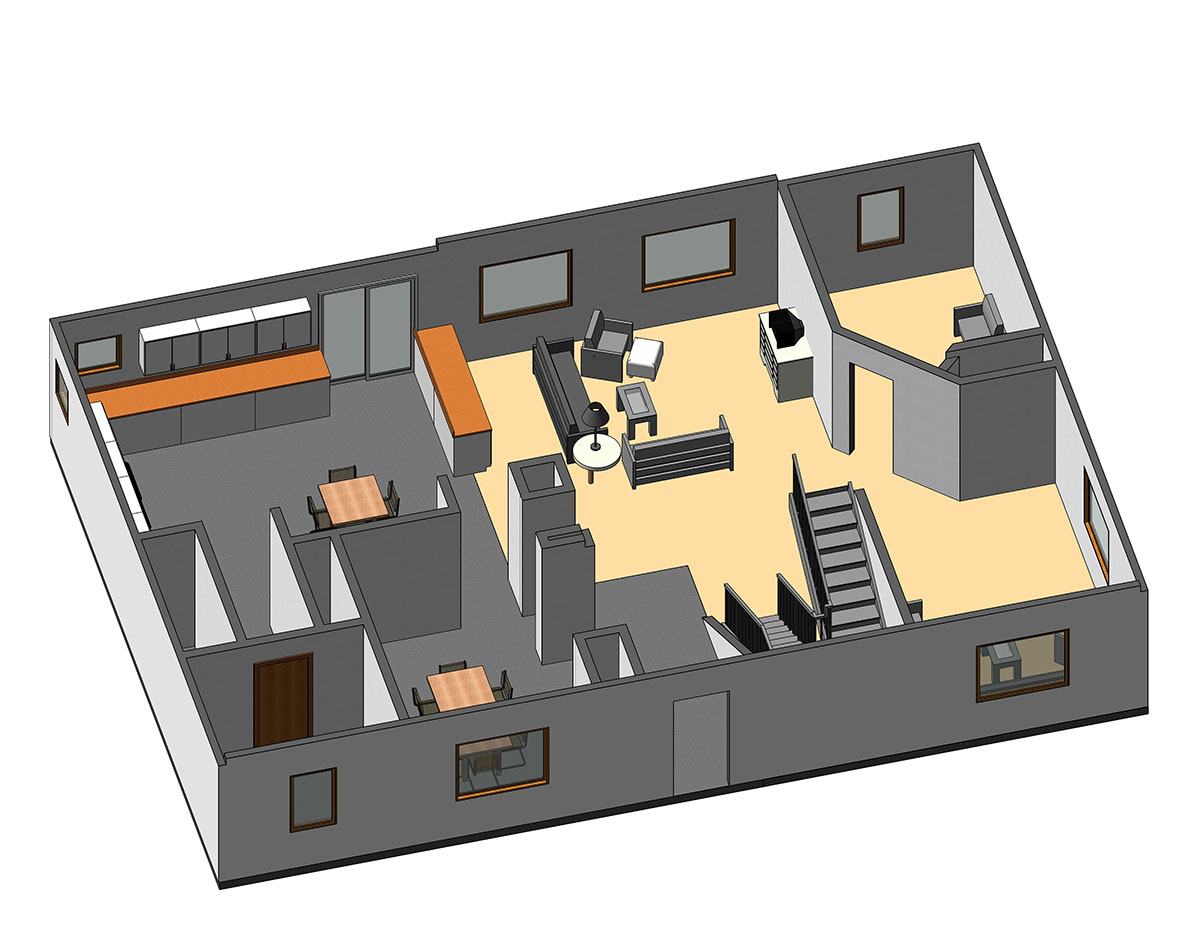
\includegraphics[width = 3in]{0_Images/Experiment_ISO/Two_Story_Base_First.jpg}} &
		\subfloat[Second Floor]{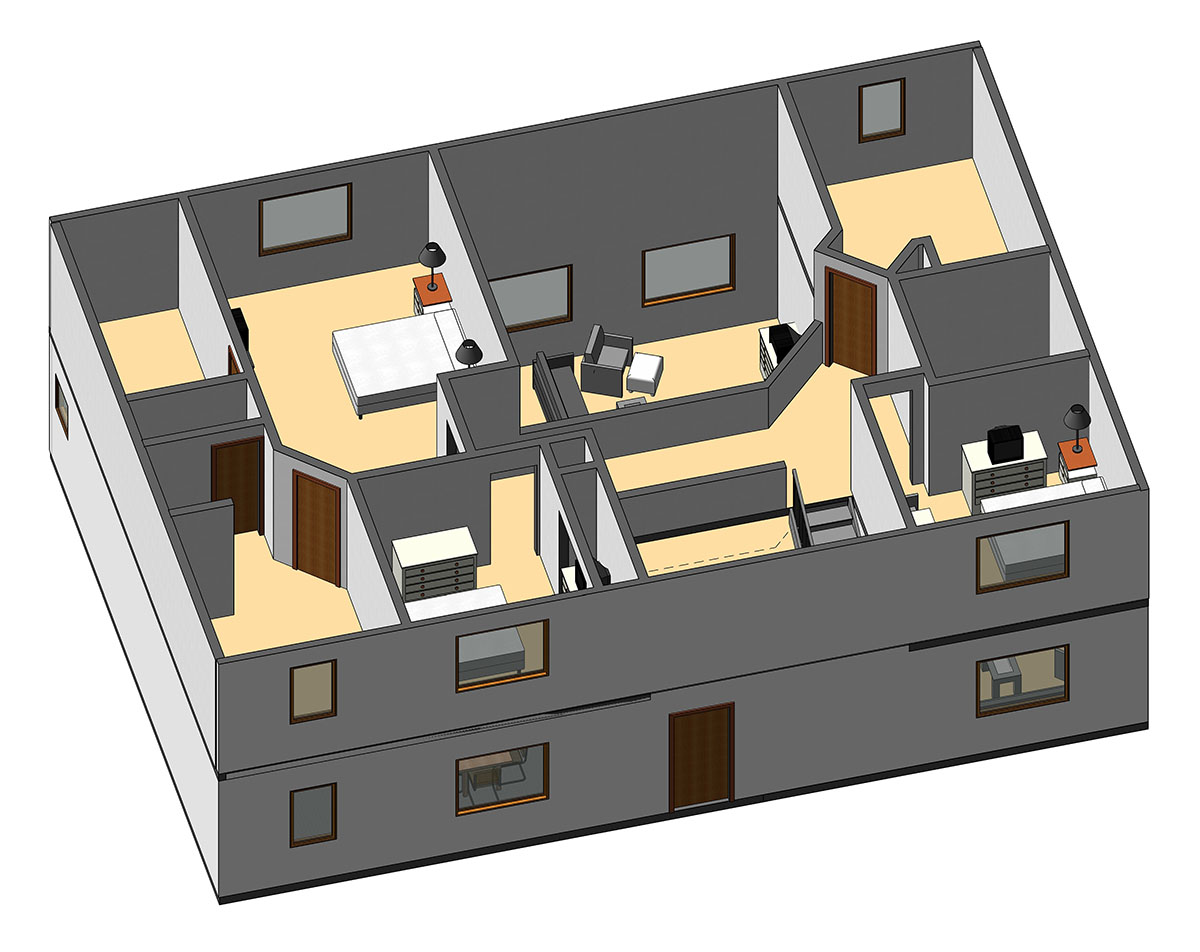
\includegraphics[width = 3in]{0_Images/Experiment_ISO/Two_Story_Base_Second.jpg}} \\
	\end{tabular}
	\caption{Two Story Isometric}
	\label{fig:TwoStoryISO}
\end{figure}

\paragraph{Air Leakage in Structures} \mbox{}

The leakage of the structures was determined through the use of a blower door test in accordance with ANSI E1872. A retotec model 5101 blower door was used in accordance with the user manual \cite{RetroTecManual}.

The standard for leakage of a structure is determined by the IECC. In 2009 the leakage for all climate zones could not exceed 7 air changes per hour. In the 2012 version of the standard the requirement was increased to less than or equal 5 air changes per hour for climate zones 1 – 2 and less than 3 air changes per hour for climate zones 3 $-$ 8.  The single story structure had a leakage rate of 25 air changes per hour and the two story had a leakage rate of 15 air changes per hour making these homes more consistent with leakage found in homes constructed prior to the 2009 IECC. 

Another measure of the leakage, Equivalent Leakage Area (ELA) was also calculated through the use of the blower door. This measurement takes into account all the leakage in a structure, as a flow, and calculates an opening size required to permit that flow. The structures used had an equivalent leakage area of 1.2 $ft^2$ for the single story and 2.4 $ft^2$ for the two story. This is equivalent to having a 15" diameter hole in the single story and a 21" diameter hole in the two story. In reality this area is distributed throughout all the smaller openings like those found around windows, however this calculation allows for the visualization of the size of opening required to provide the leakage rate found in the test fixtures utilized. 

\subsection{Furnishings}

Furniture was acquired for the experiments such that each room of furniture was the same from experiment to experiment. Descriptions, dimensions and weights for all of the furniture used are in Table \ref{FurnitureTable}. Images of each piece of furniture can be seen in Figure \ref{fig:FurnitureImages}.

\renewcommand{\arraystretch}{1.5}
\begin{table}[H]
	\centering
	\caption{Furniture Dimensions and Weight}
		\begin{tabular}[c]{|c|c|c|c|c|}
			\hline
			\textbf{Item} & \textbf{Length (in.)} & \textbf{Width (in.)} & \textbf{Height (in.)} & \textbf{Weight (lbs.)} \\ \hline \hline
			Kitchen Table & 30 & 30 & 30 & 45.2 \\ \hline
			Kitchen Table Chair & 17.5 & 19 & 33 & 15.5 \\ \hline
			Night Stand & 27 & 17 & 23.5 & 59.3 \\ \hline
			Full Box Spring & 79 & 52.5 & 9 & 42.1 \\ \hline
			Full Mattress & 80 & 53 & 8 & 53 \\ \hline
			Comforter & 92 & 104 & - & - \\ \hline
			Standard Pillow & 24 & 16 & 3 & 1.5 \\ \hline
			Flat Sheet & 98 & 83 & - & 3.5 \\ \hline
			Headboard & 54 & 18 & 2.5 & 34.1 \\ \hline
			Dresser & 44.5 & 24 & 35.5 & 212.6 \\ \hline
			Foot Stool & 23 & 18 & 16.5 & 16.1 \\ \hline
			Round End Table & 24 & 24 & 22 & 32.3 \\ \hline
			Coffee Table & 30 & 18 & 18 & 25 \\ \hline
			Lamp \& Shade & 12 & 12 & 22 & 6.3 \\ \hline
			Chair (Yellow) & 30 & 30.5 & 34 & 34.8 \\ \hline
			Chair (Brown) & 32 & 32 & 33 & 82.1 \\ \hline
			Sleeper Sofa (Green) & 84 & 36.5 & 33 & 208 \\ \hline
			Sleeper Sofa (Orange) & 65 &35.5 & 31.5 & 145.1 \\ \hline
			Curtain & - & 225 & 100 & 18 \\ \hline	
			Base Kitchen Cabinet & 36 & 24 & 34.5 & 70.7 \\ \hline
			Wall Kitchen Cabinet & 25 & 12 & 30 & 34.6 \\ \hline
		\end{tabular}
	\label{FurnitureTable}
\end{table}

\begin{figure}
	\centering
	\begin{tabular}[c]{c c c c}
		\subfloat[Kitchen Table]{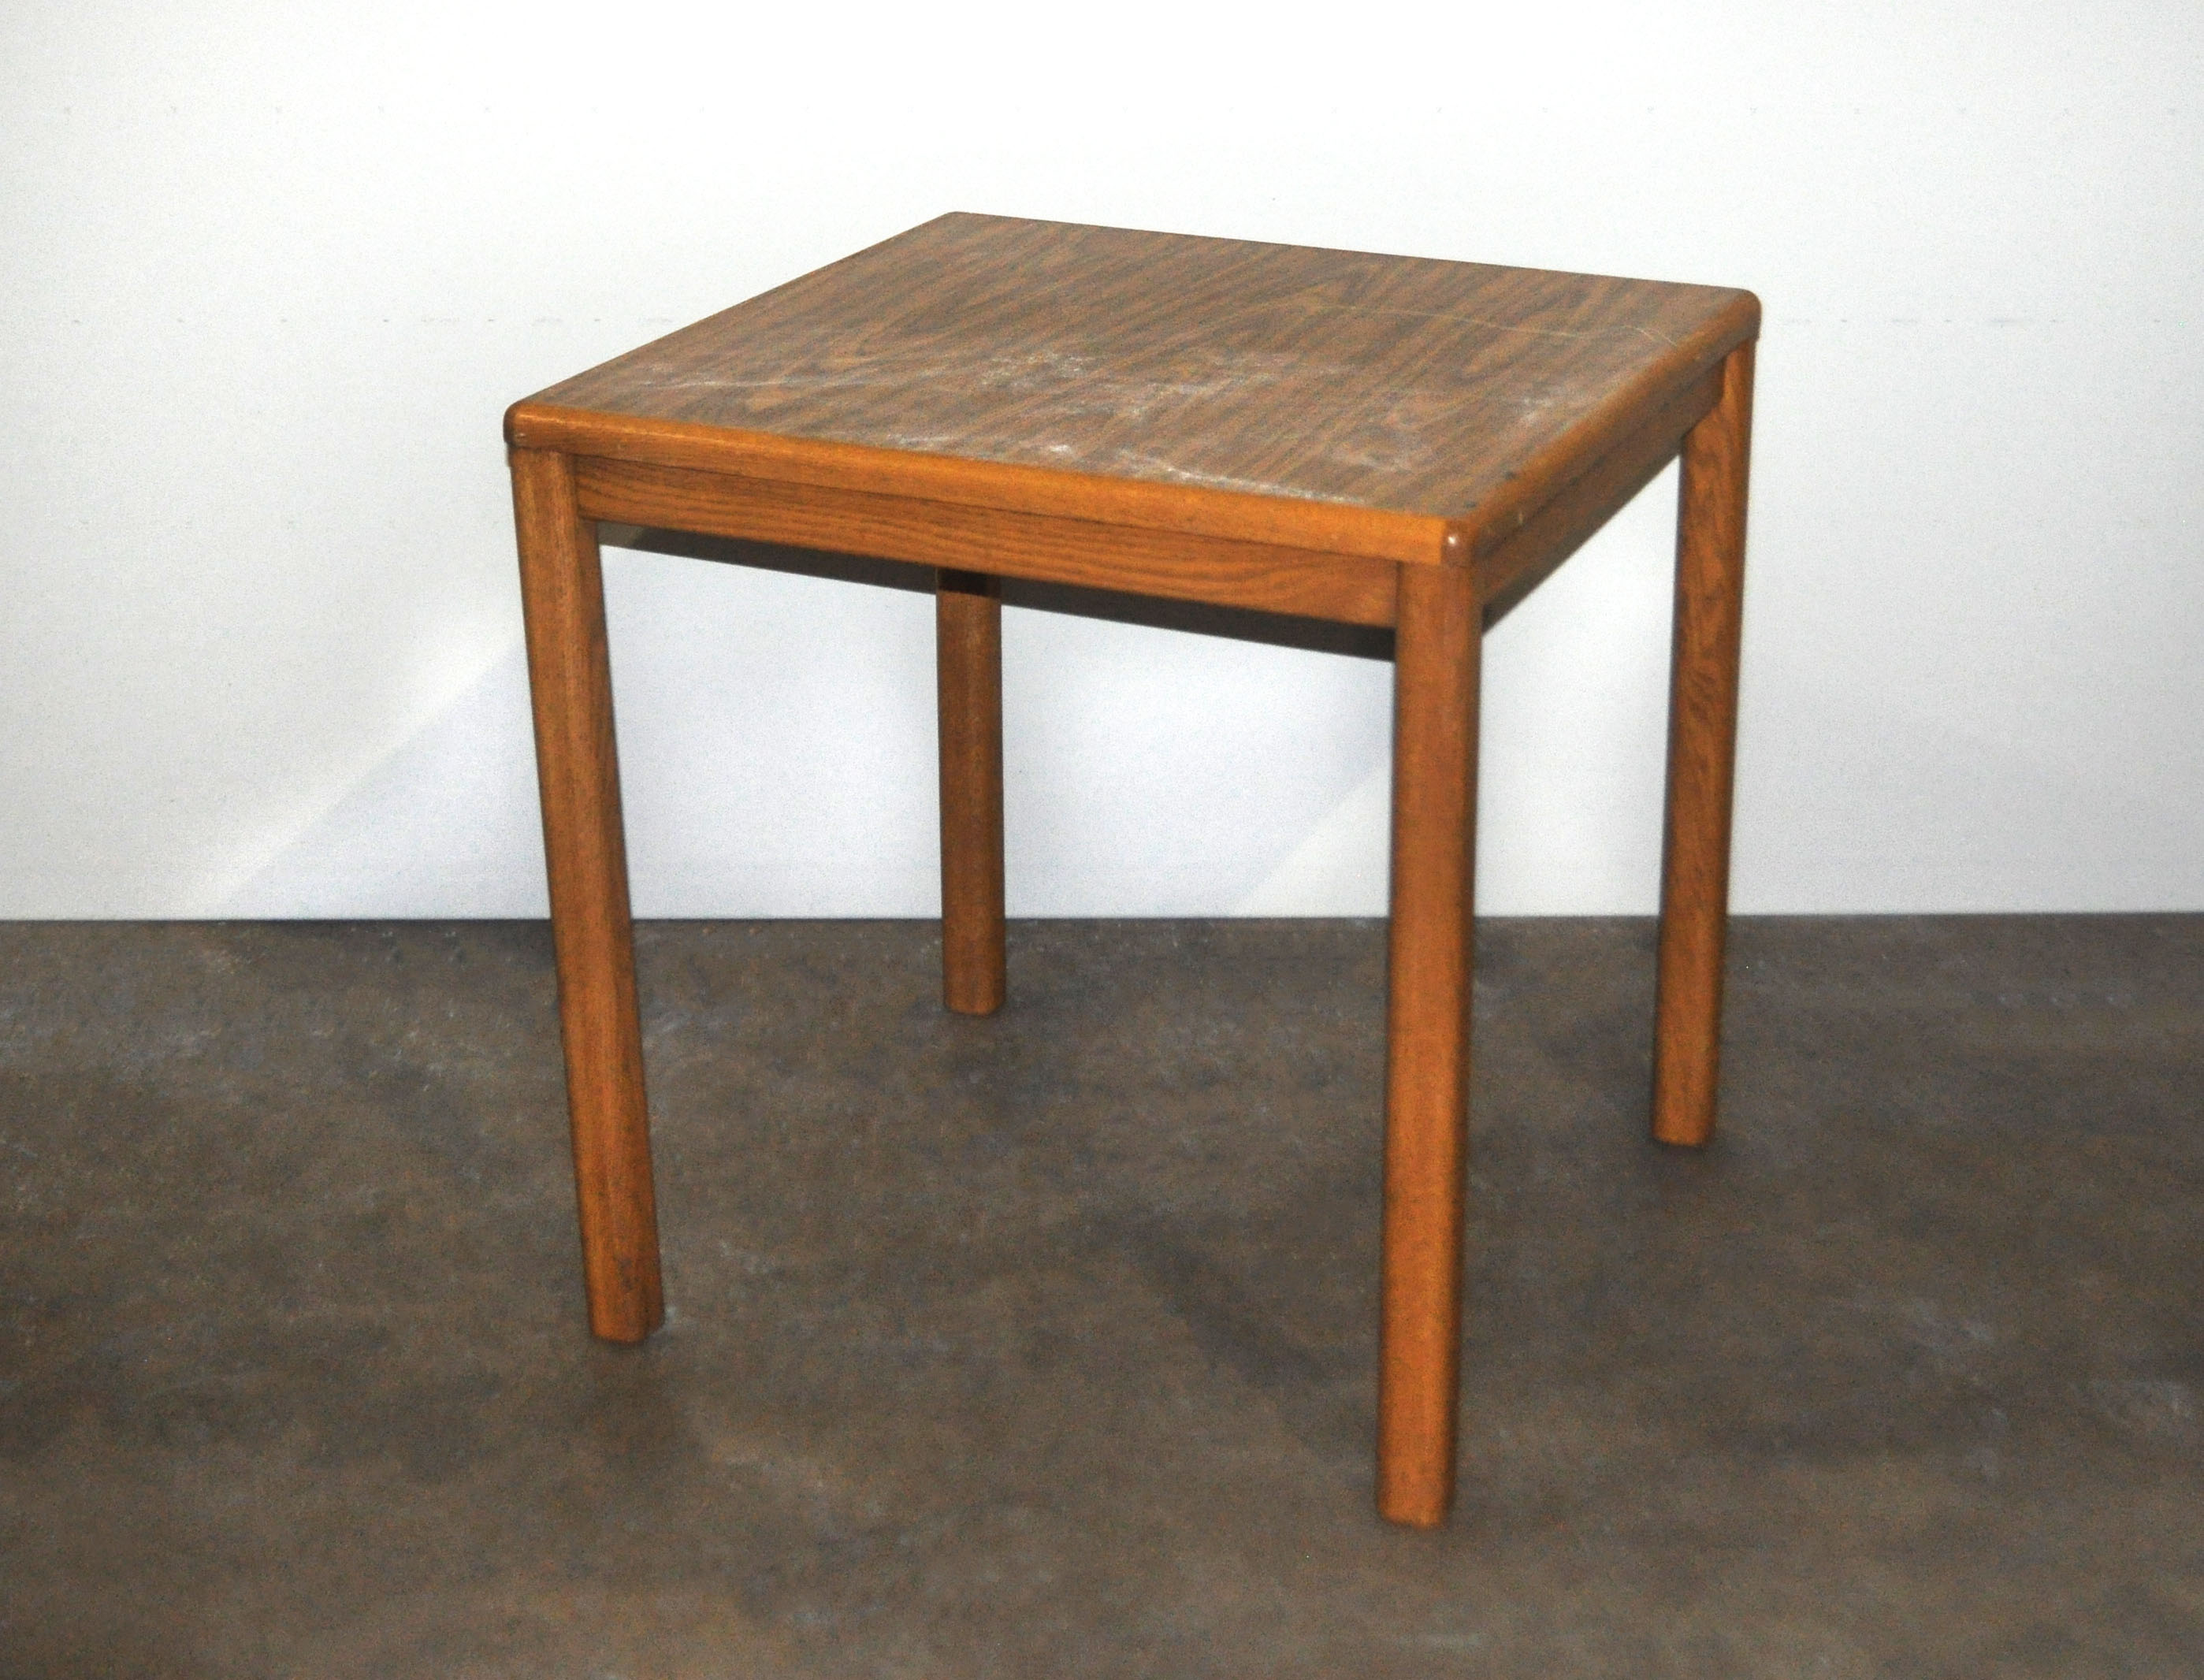
\includegraphics[width=3cm]{0_Images/Furniture/KitchenTable.jpg}} &
		\subfloat[Kitchen Chair]{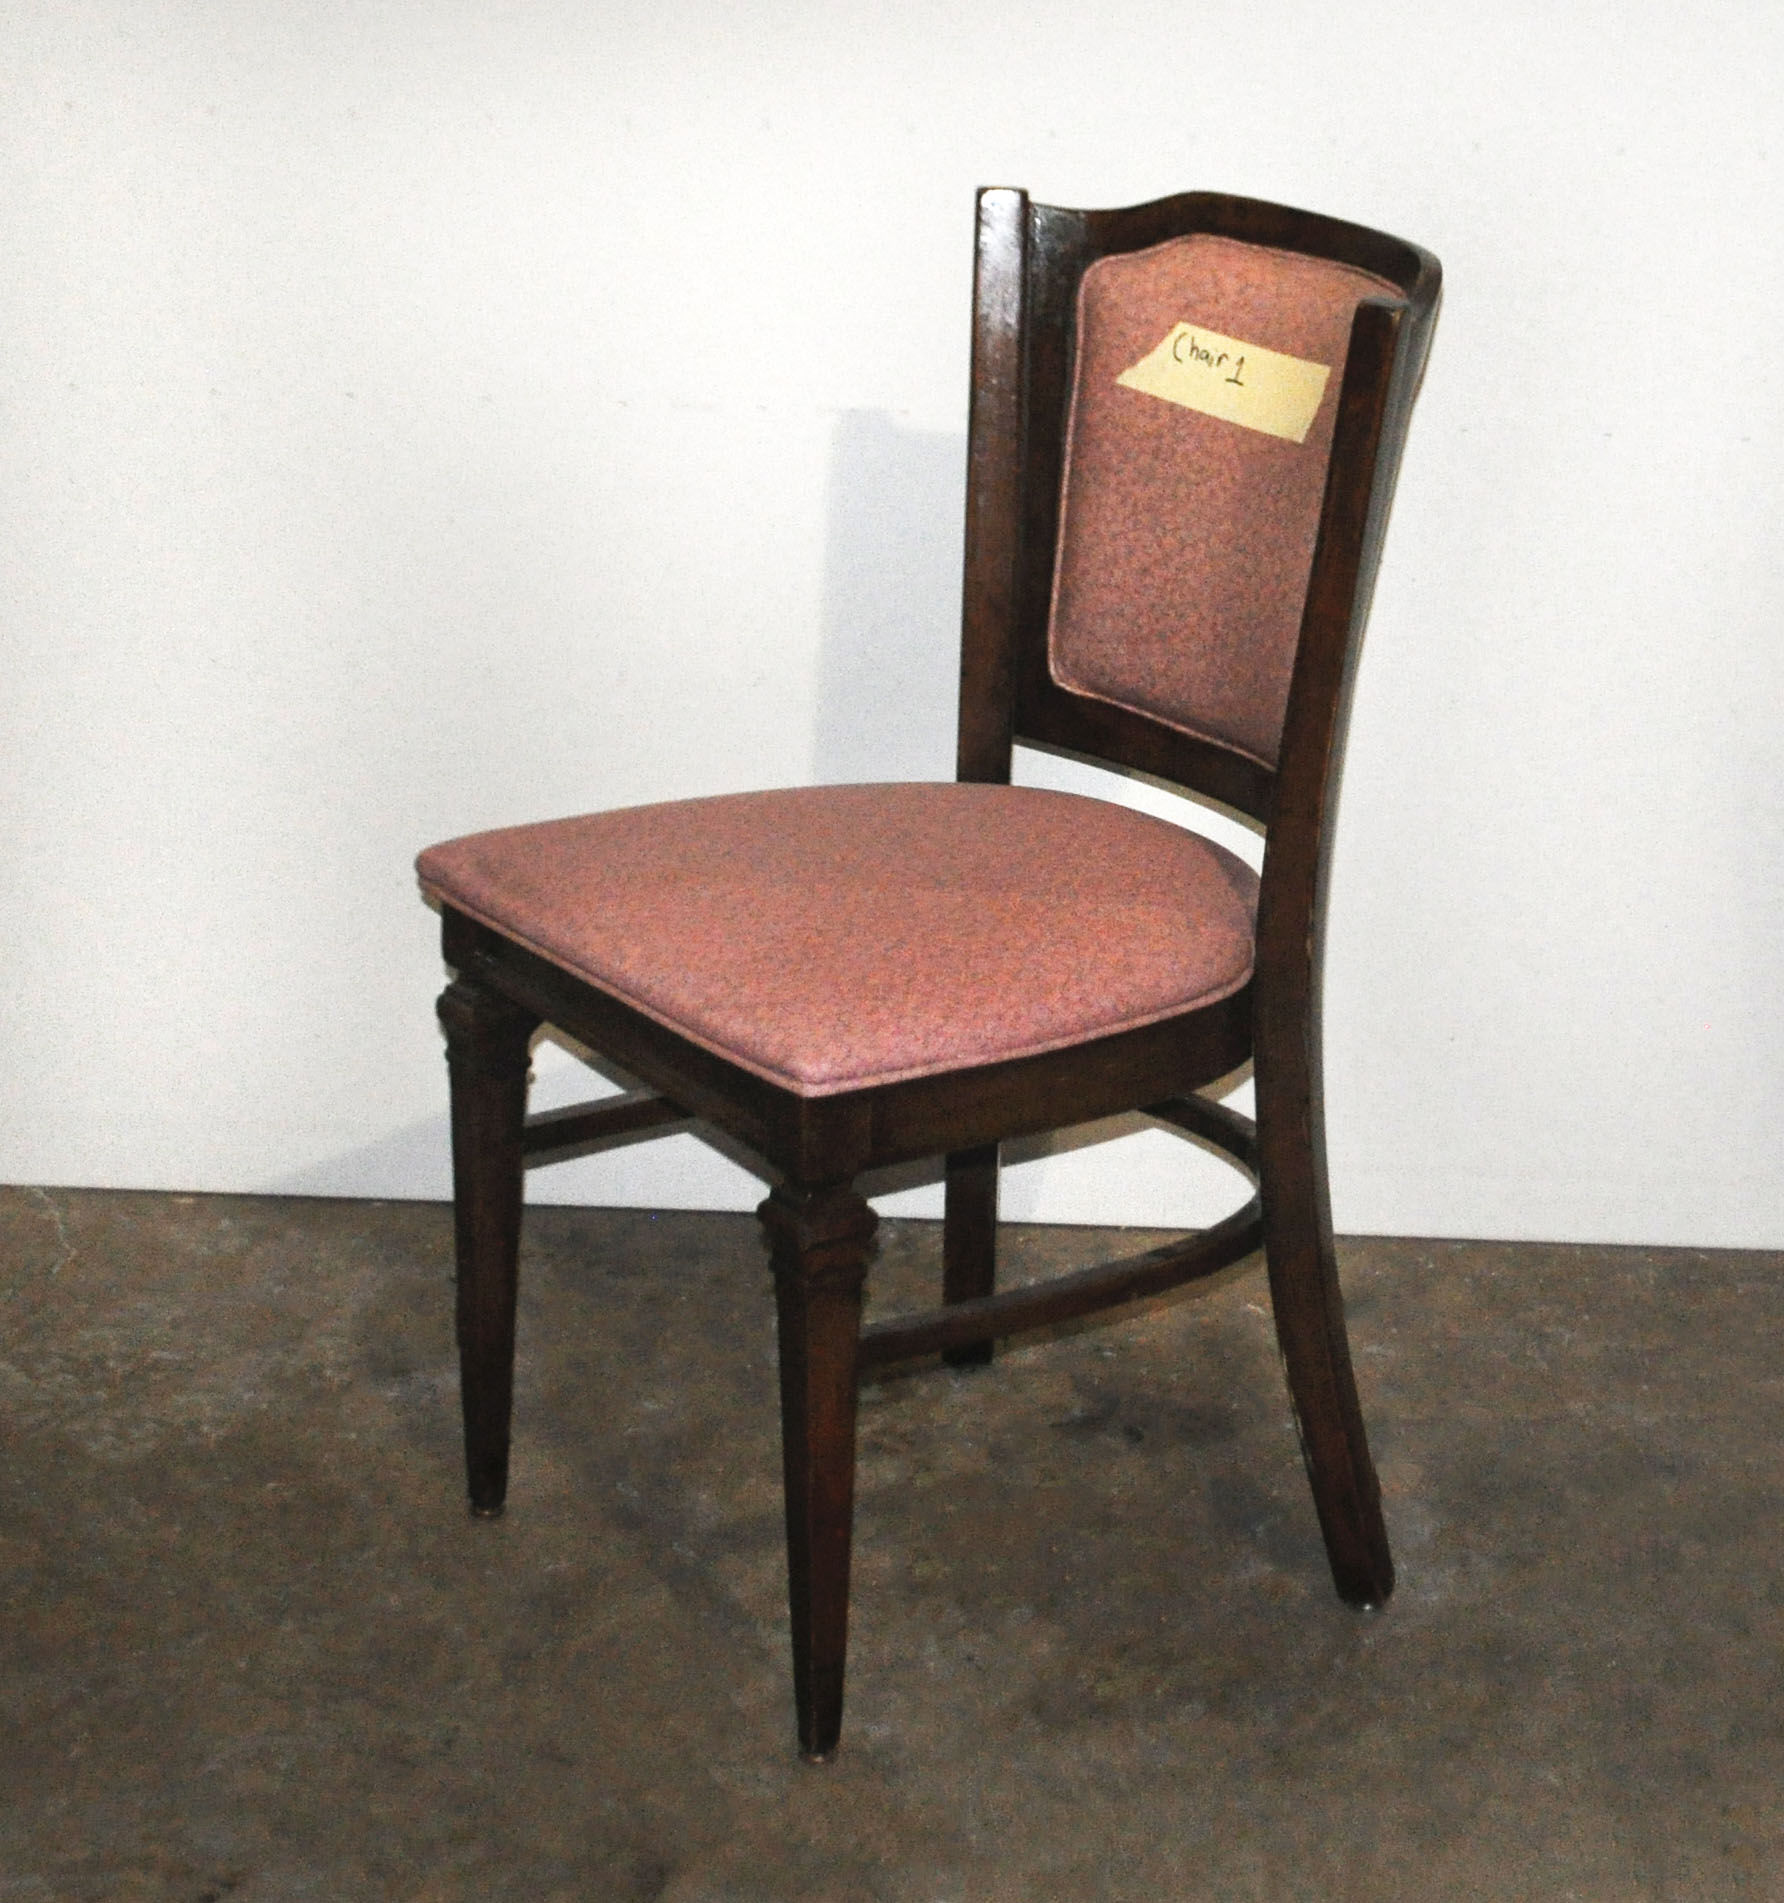
\includegraphics[width=3cm]{0_Images/Furniture/KitchenTableChair.jpg}} &
		\subfloat[Night Stand]{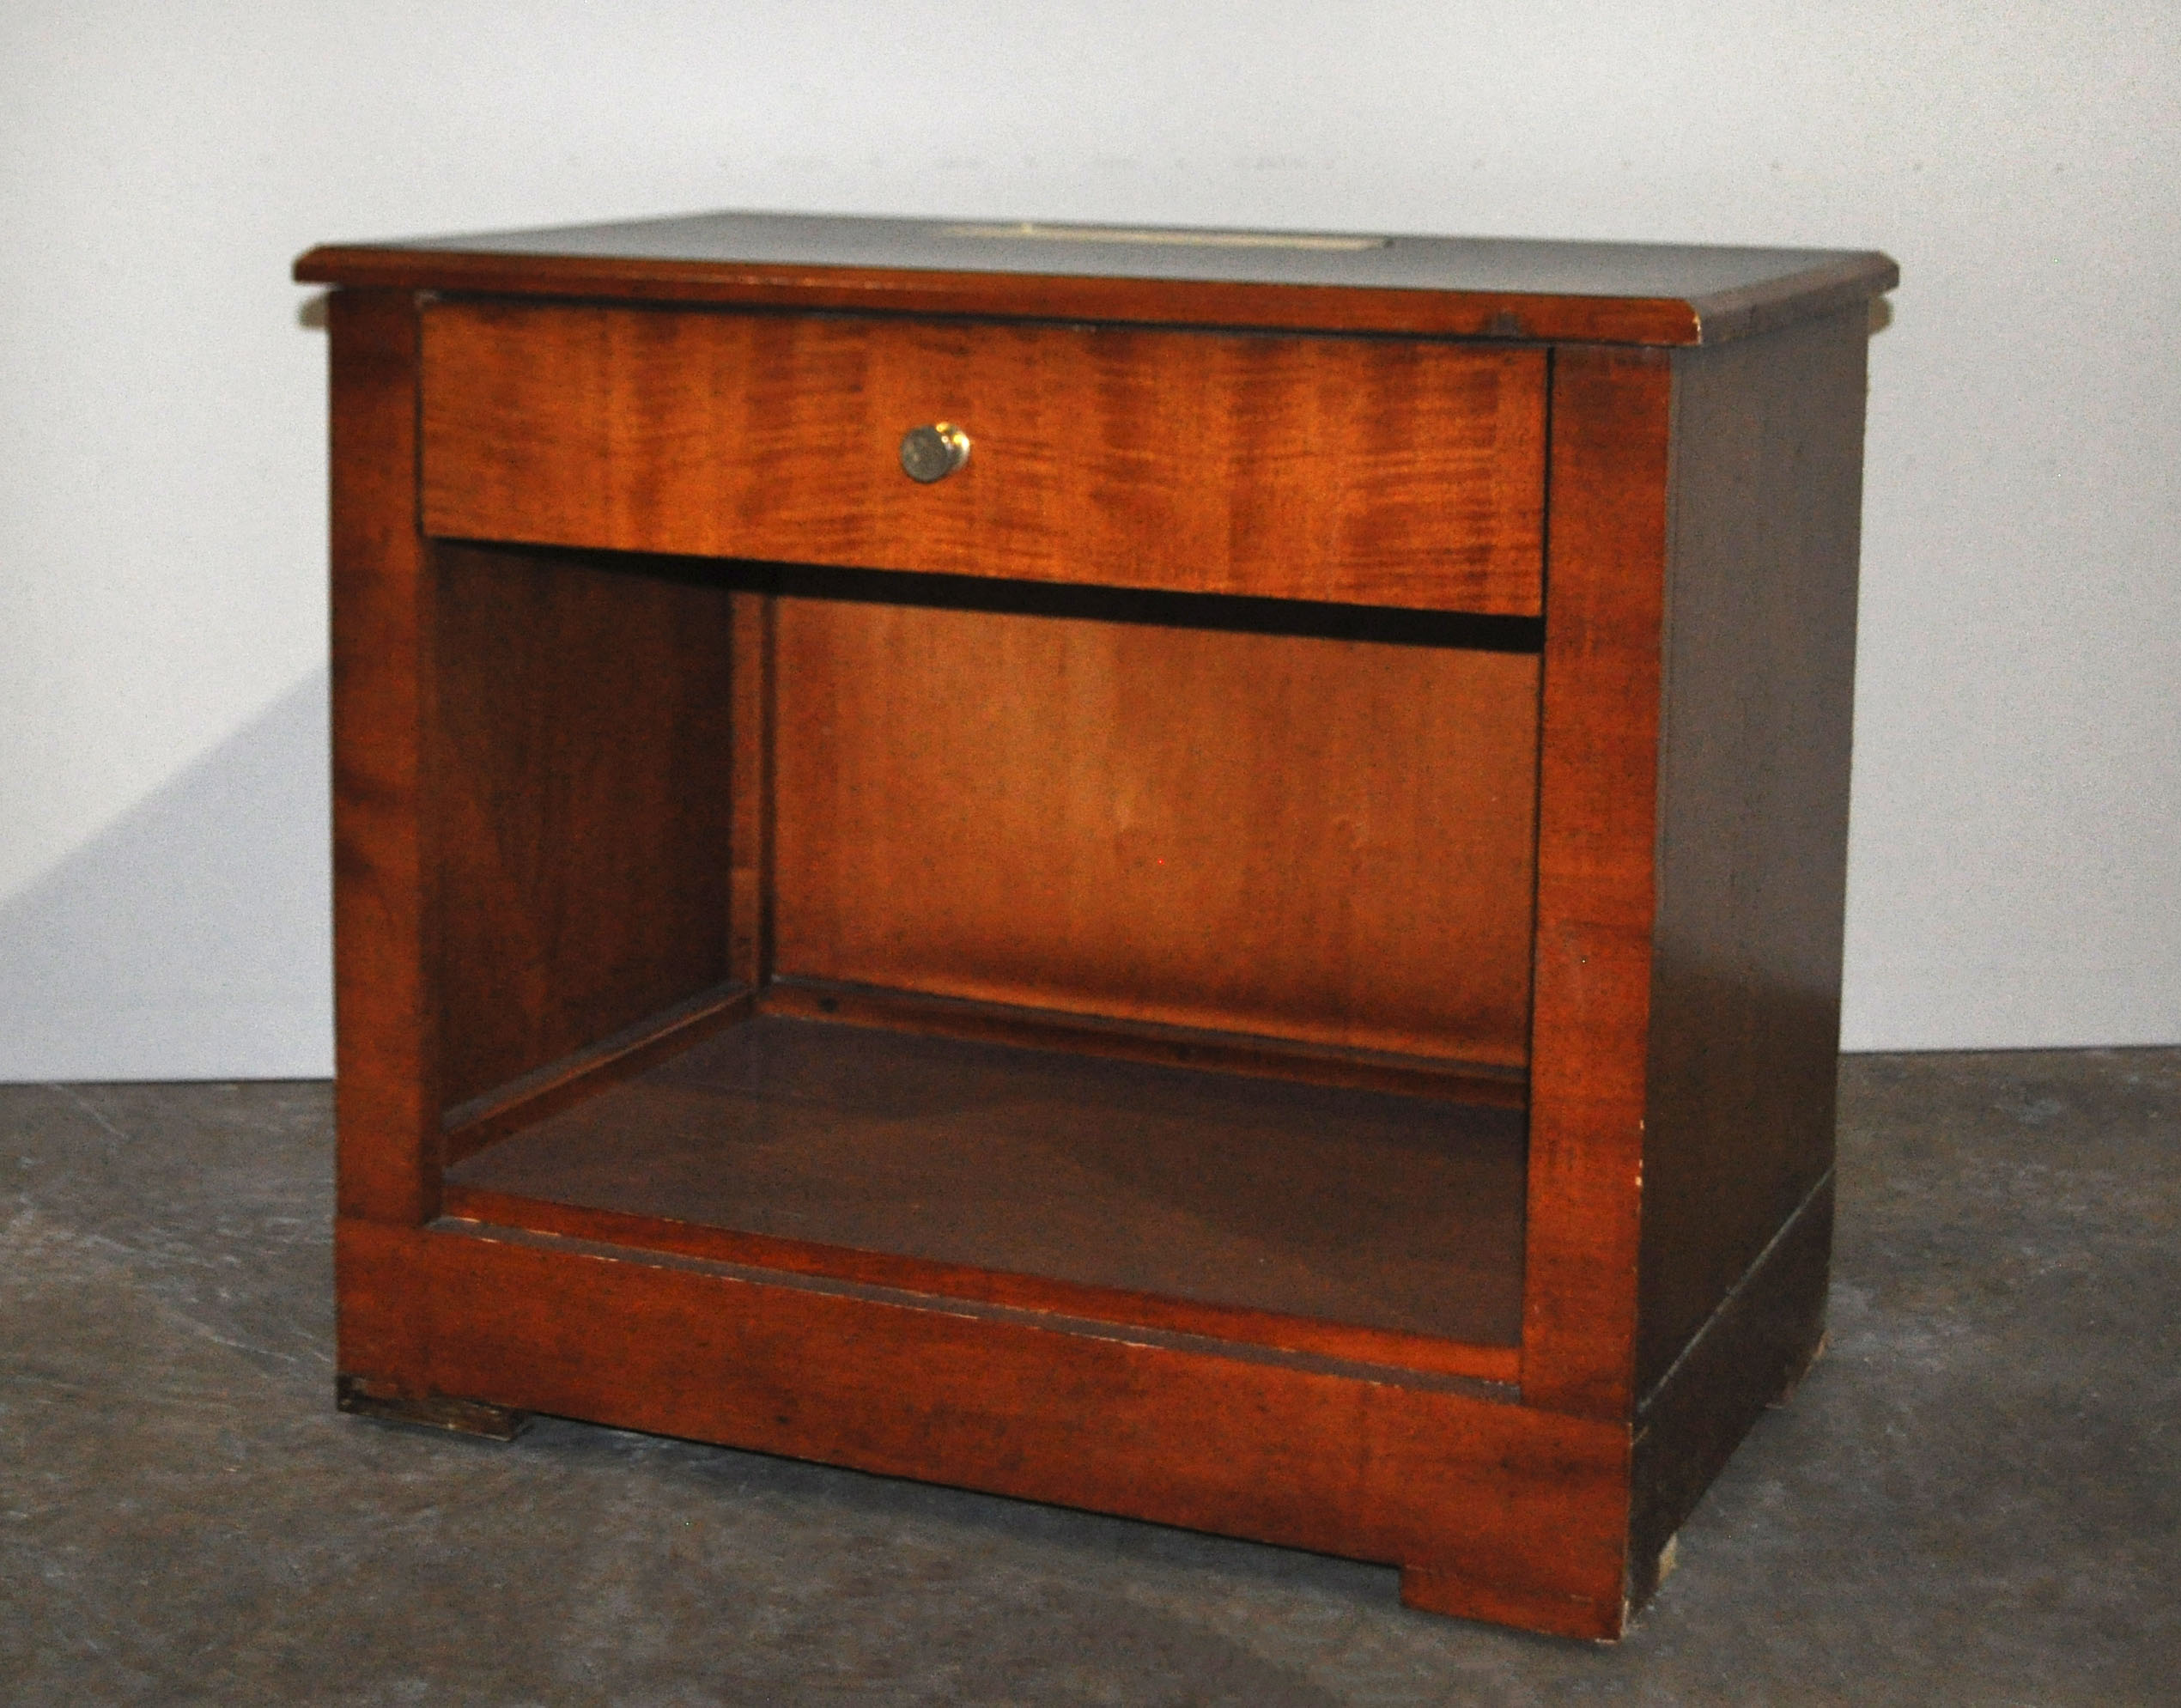
\includegraphics[width=3cm]{0_Images/Furniture/NightStand.jpg}} &
		\subfloat[Box Spring]{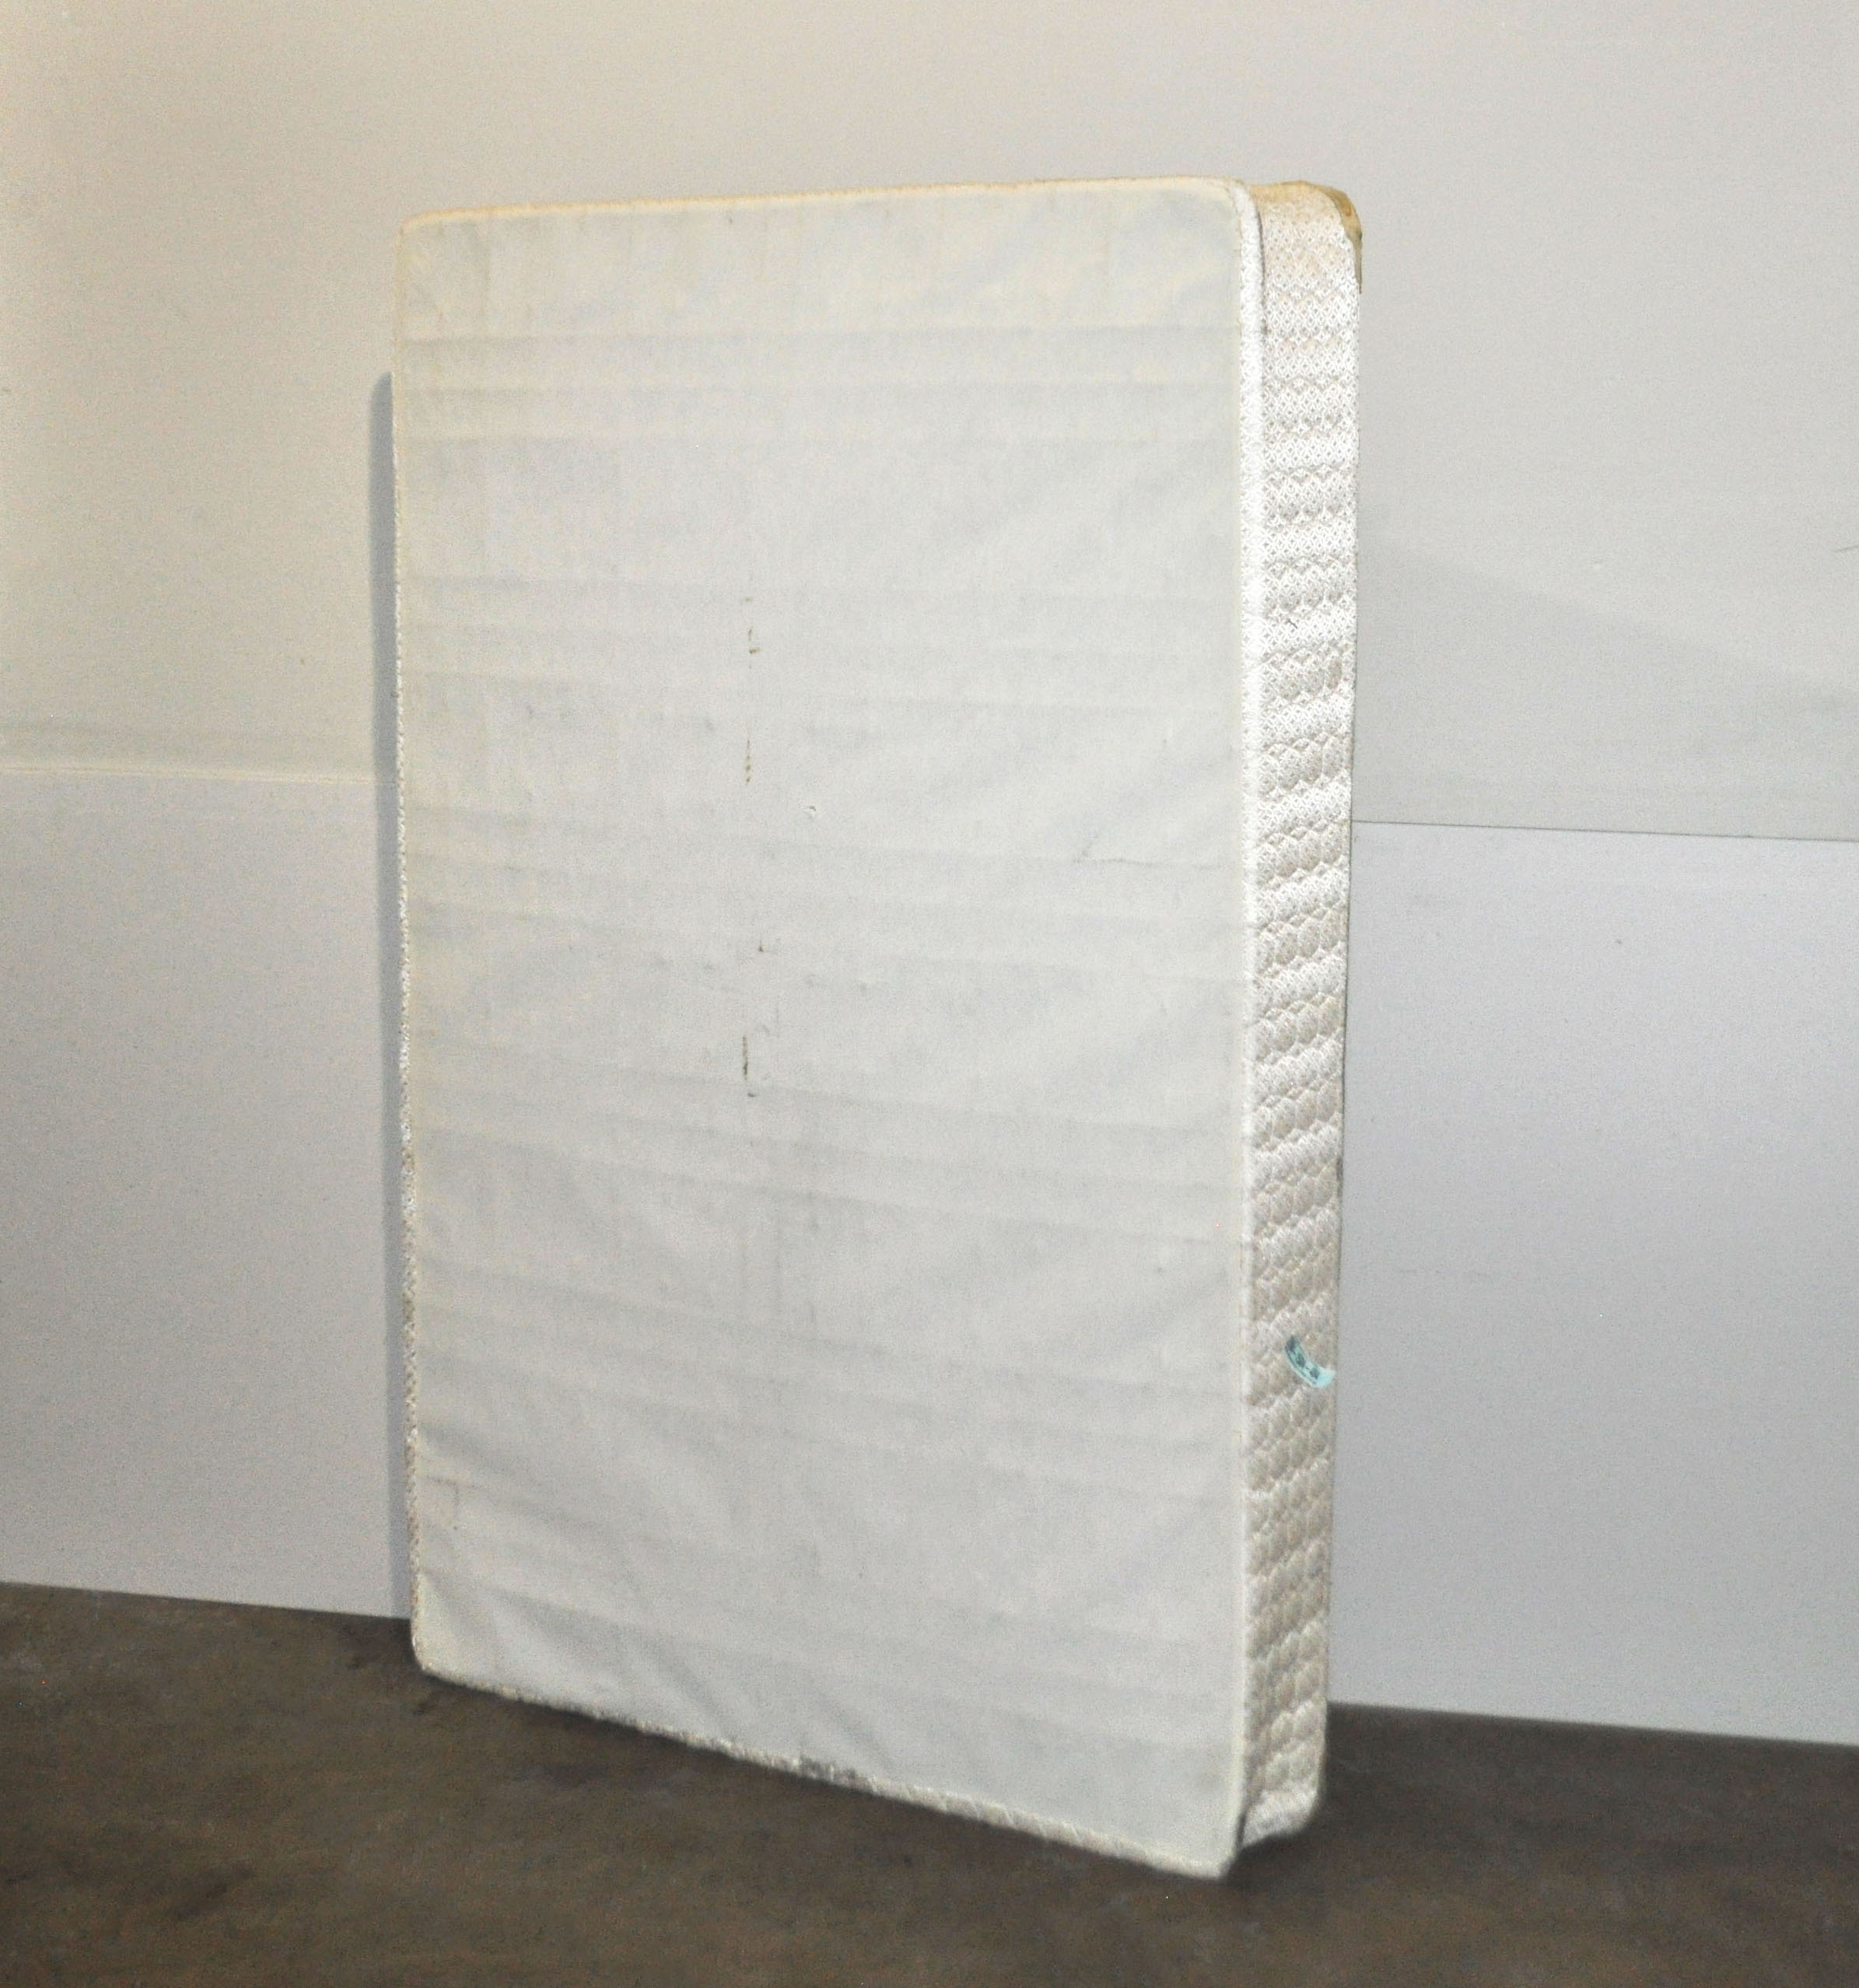
\includegraphics[width=3cm]{0_Images/Furniture/BoxSpring.jpg}} \\
		\subfloat[Matress]{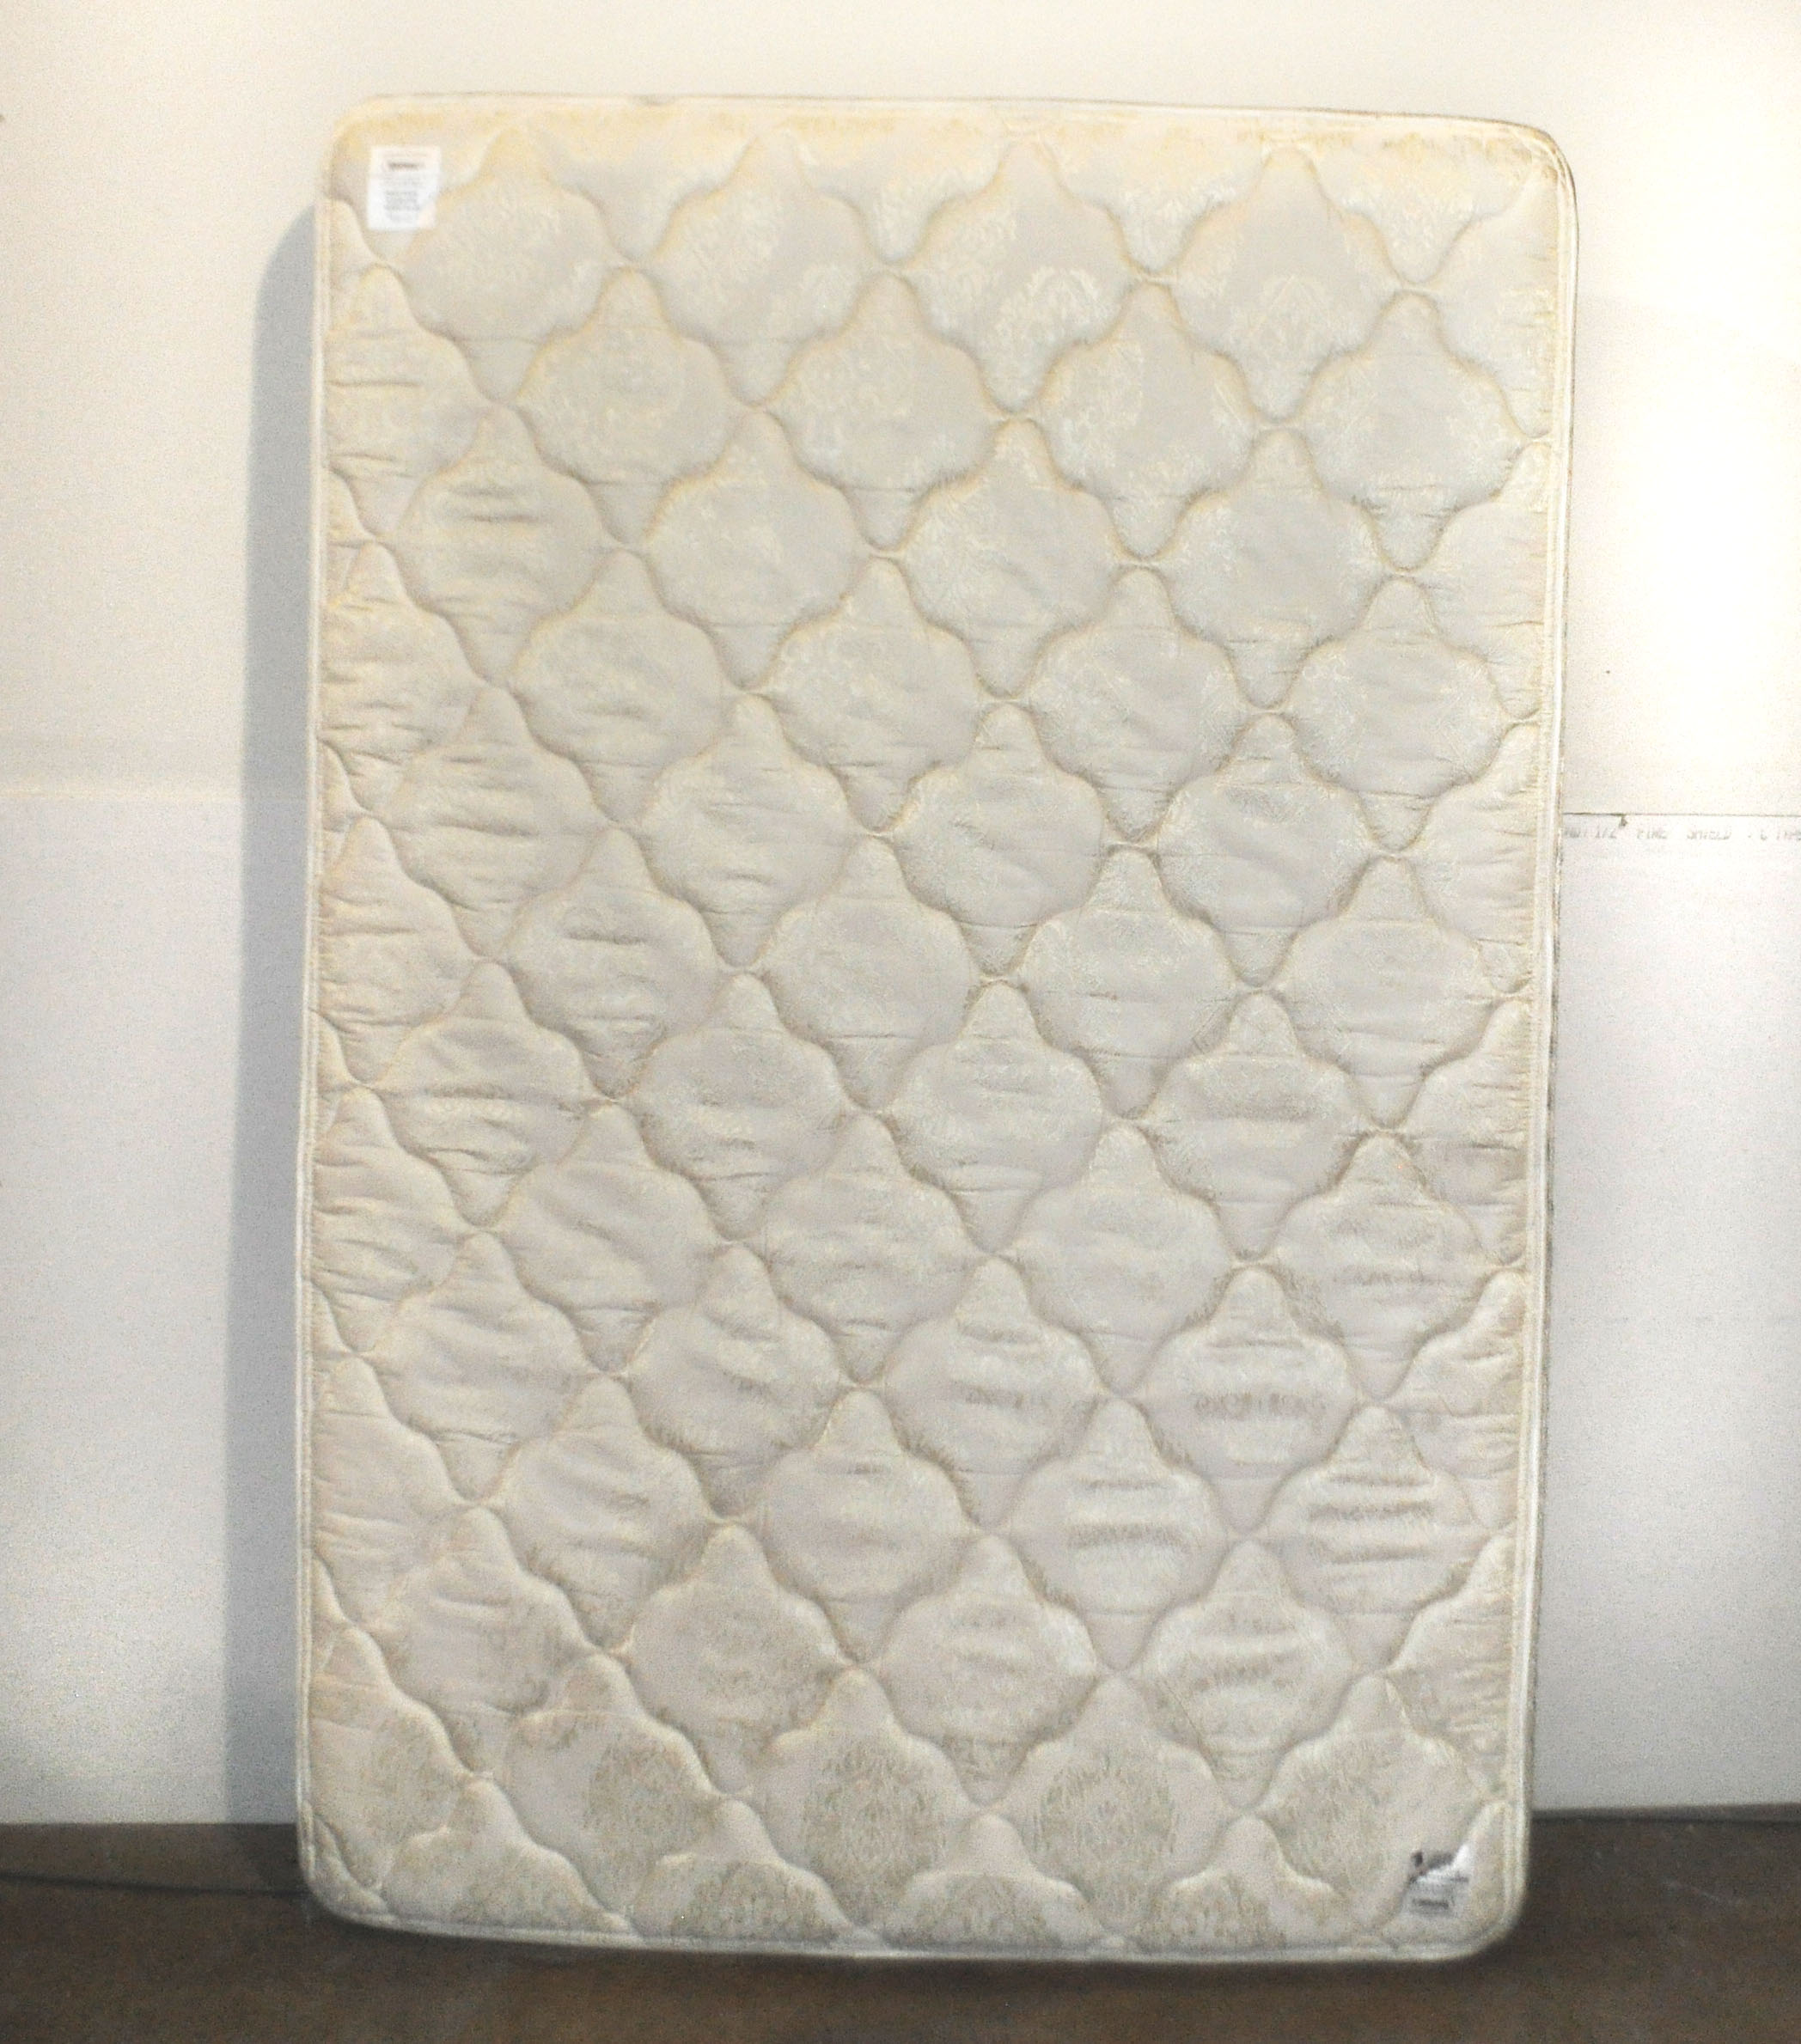
\includegraphics[width=3cm]{0_Images/Furniture/Matress.jpg}} &
		\subfloat[Head Board]{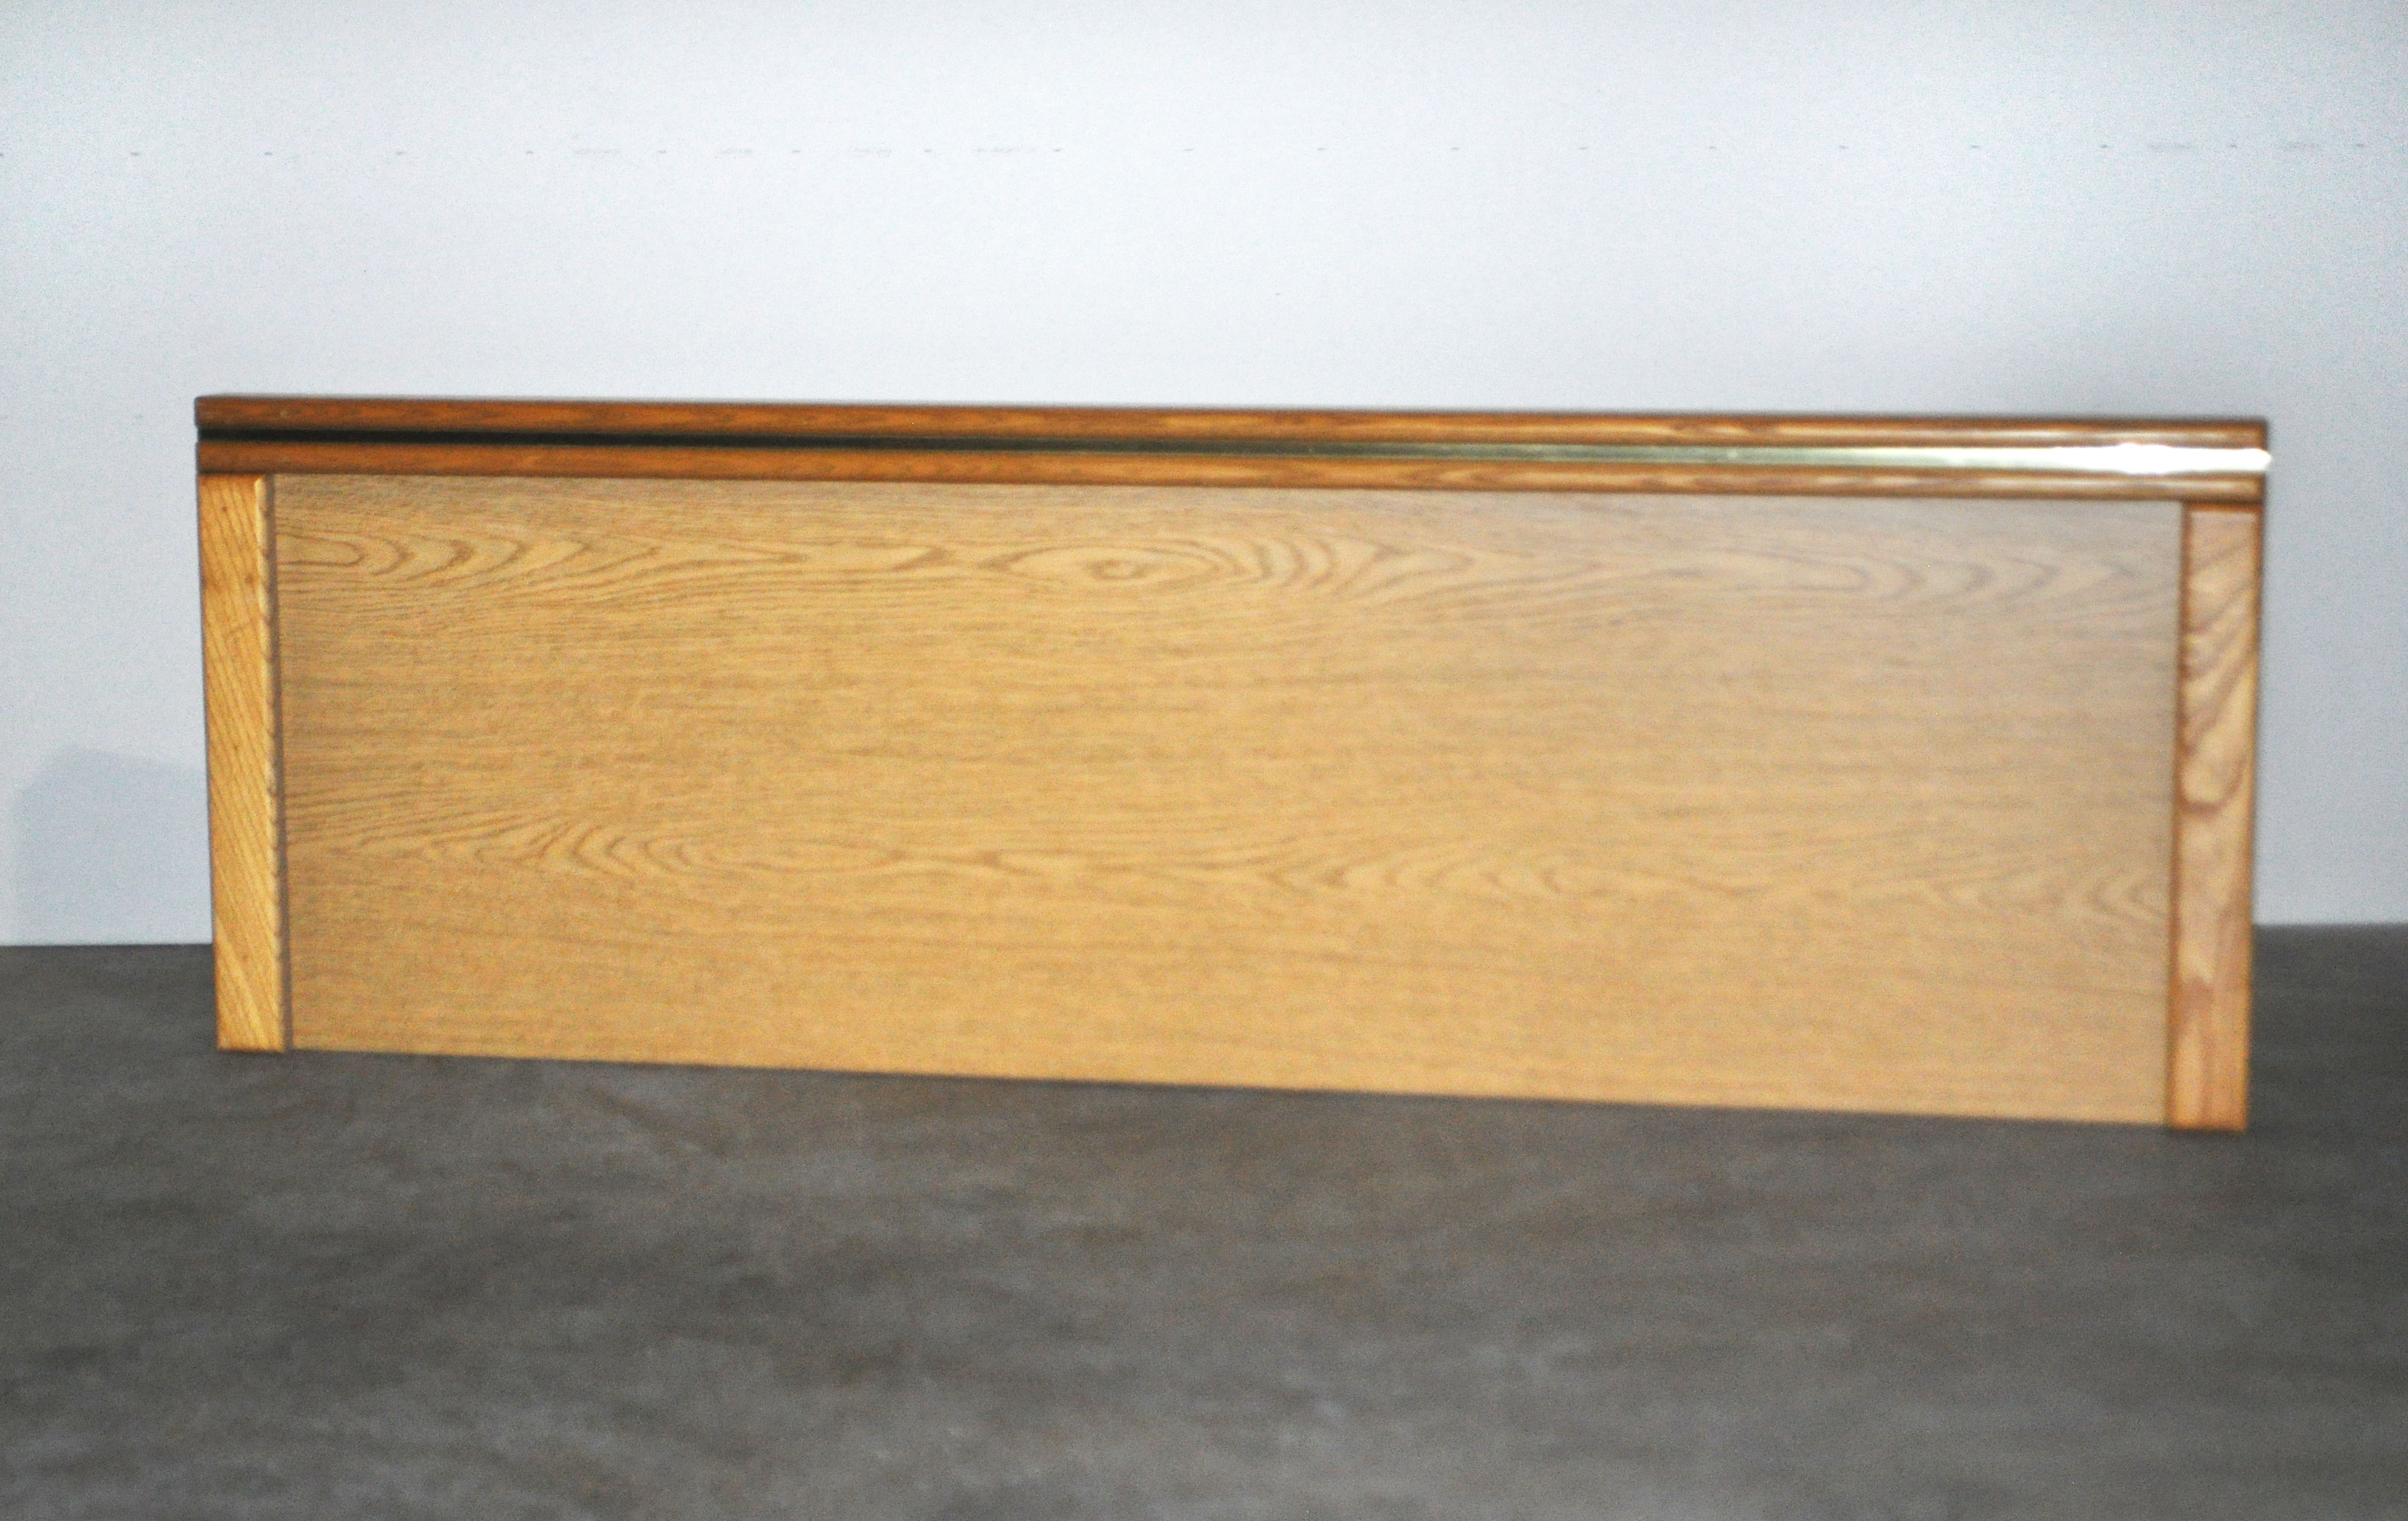
\includegraphics[width=3cm]{0_Images/Furniture/HeadBoard.jpg}} &
		\subfloat[Dresser]{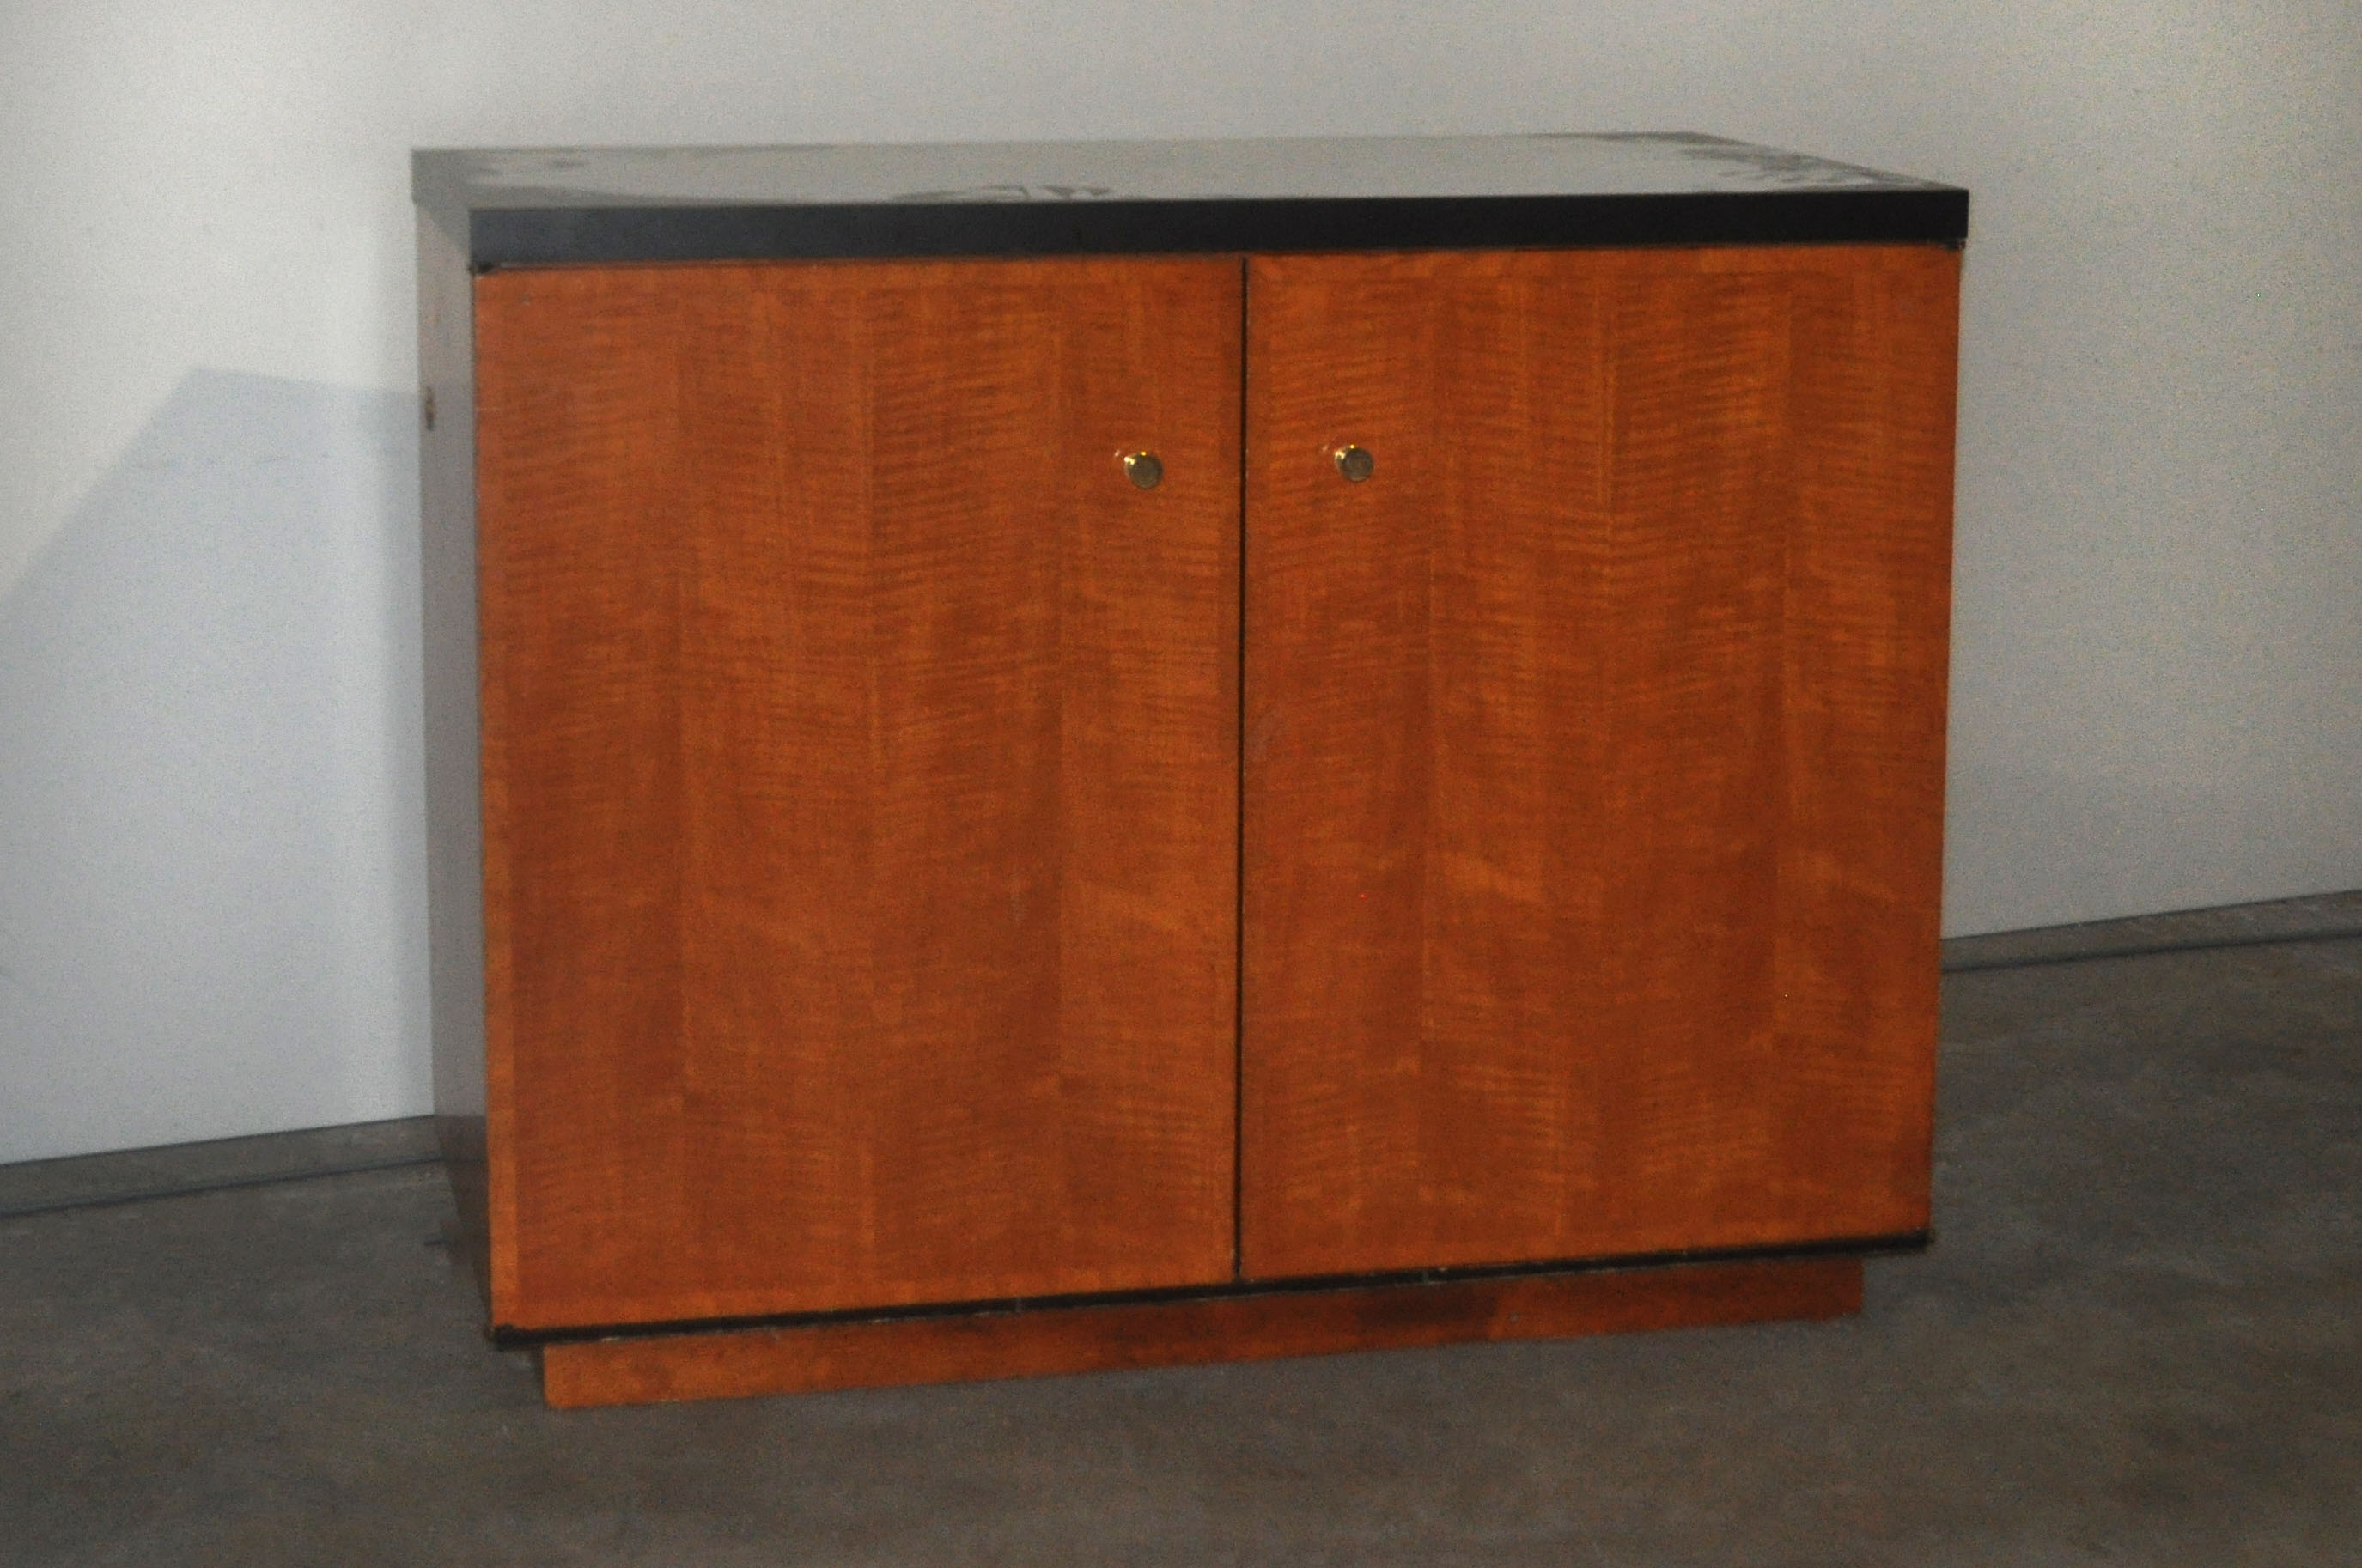
\includegraphics[width=3cm]{0_Images/Furniture/Dresser_TVStand.jpg}} &
		\subfloat[Foot Stool]{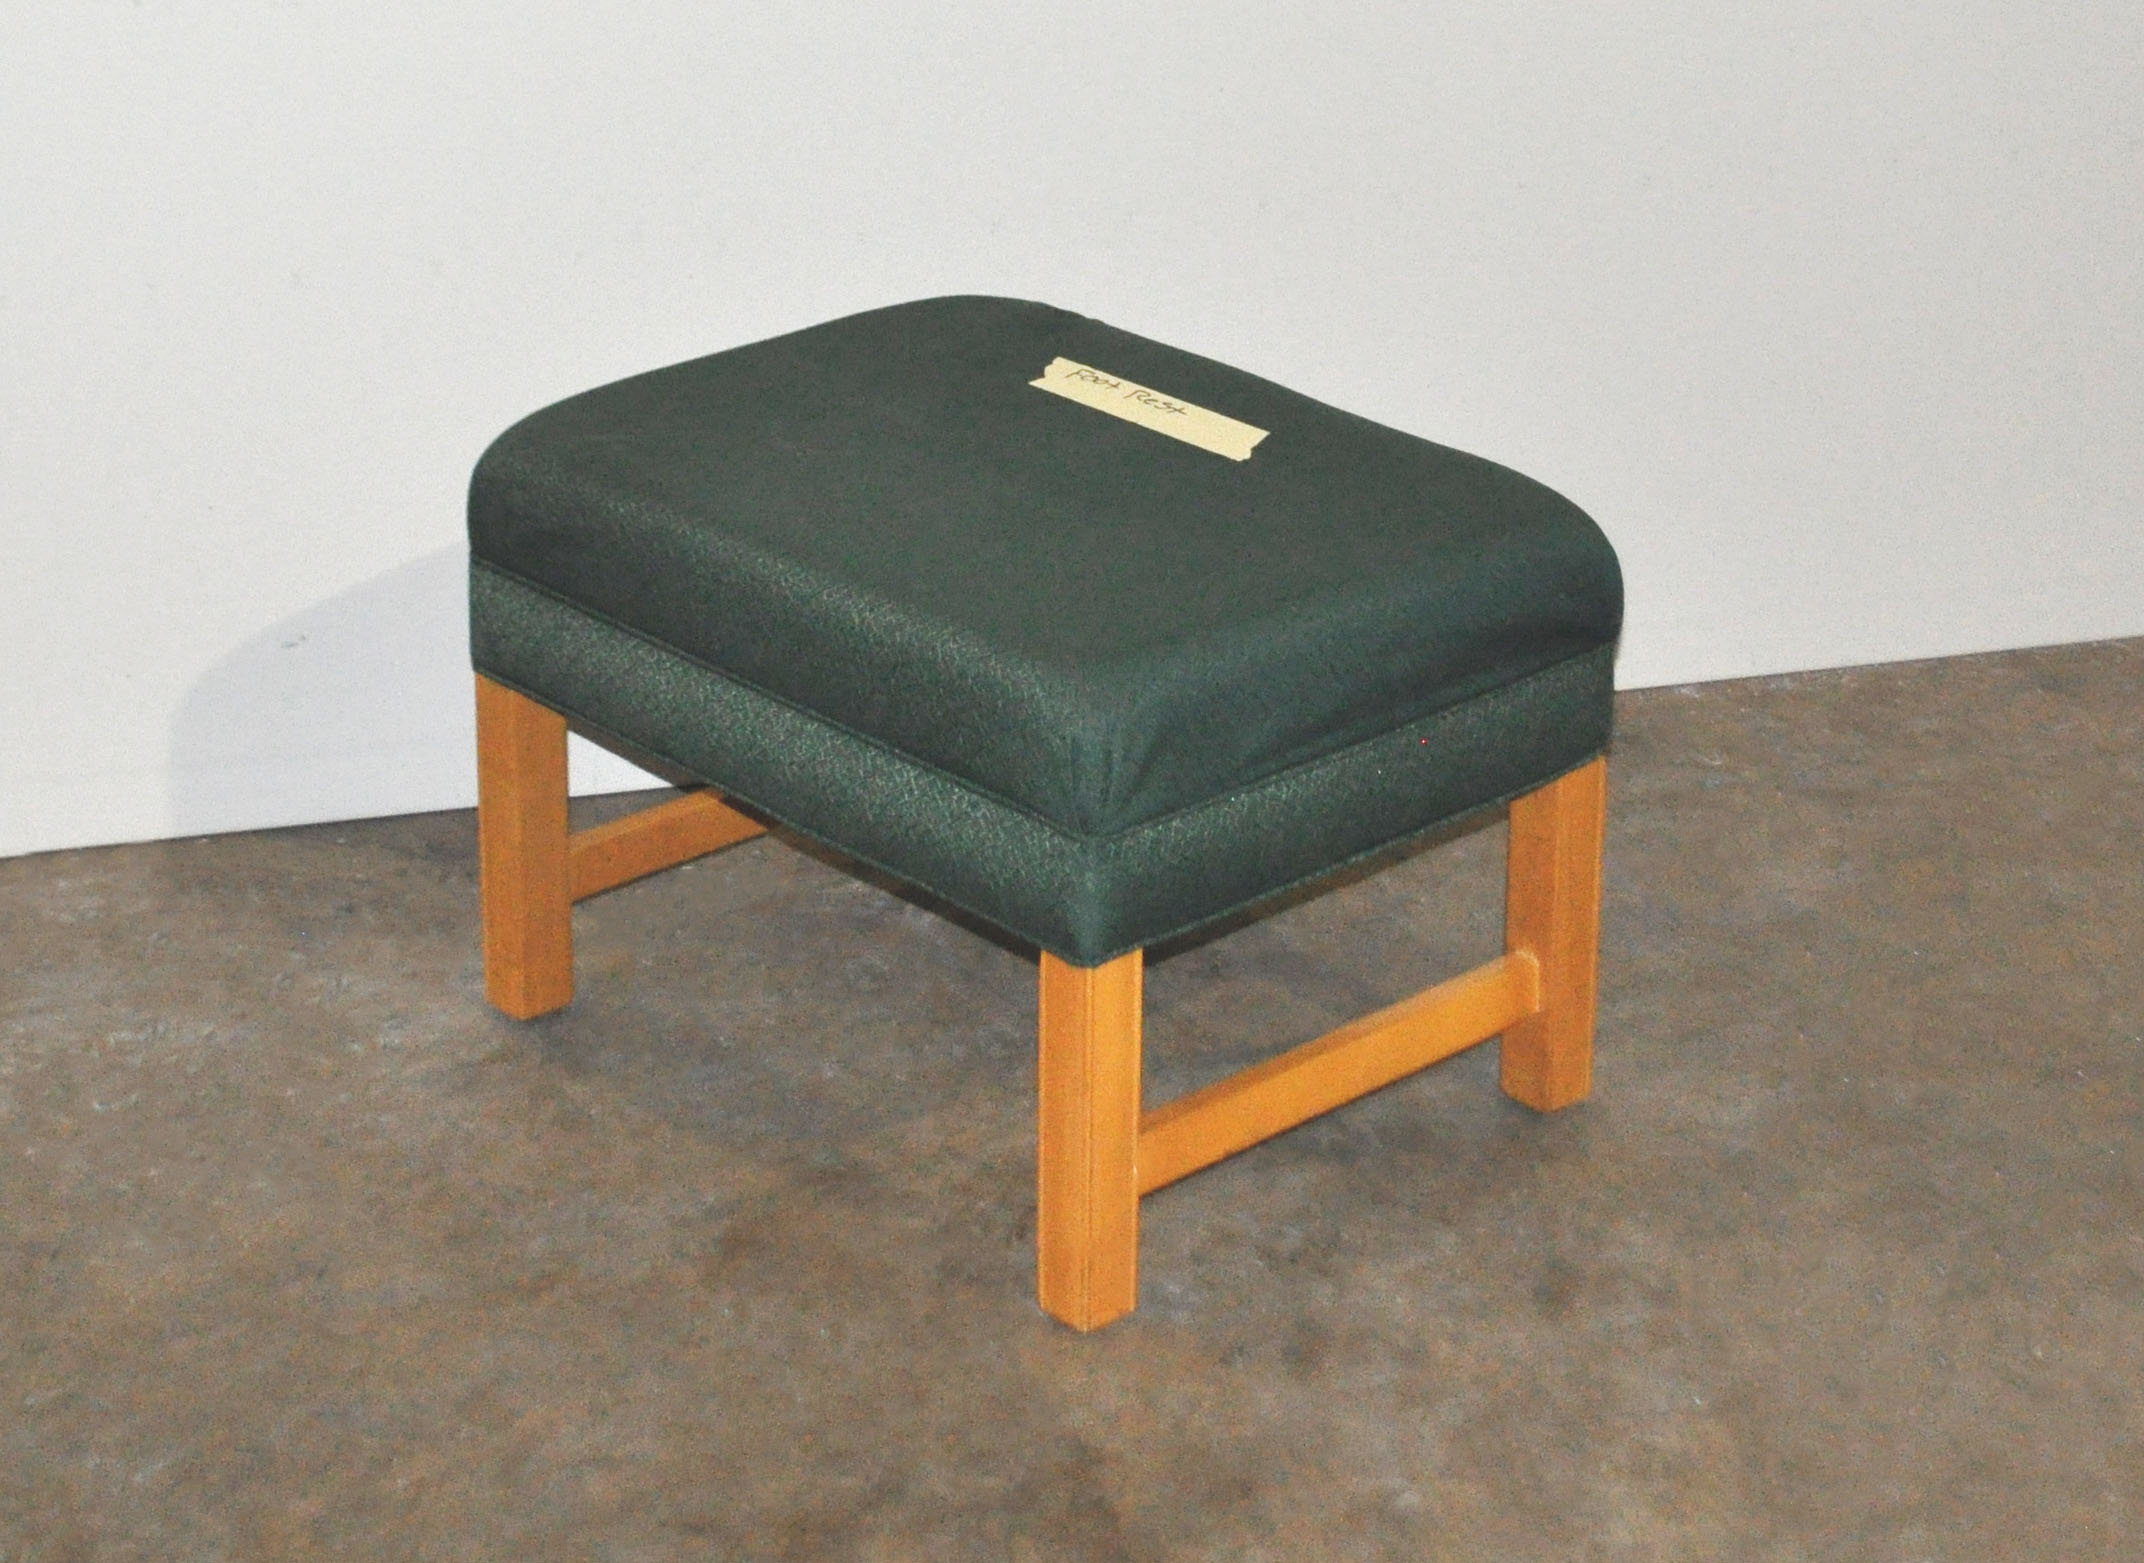
\includegraphics[width=3cm]{0_Images/Furniture/FootStool.jpg}} \\
		\subfloat[End Table]{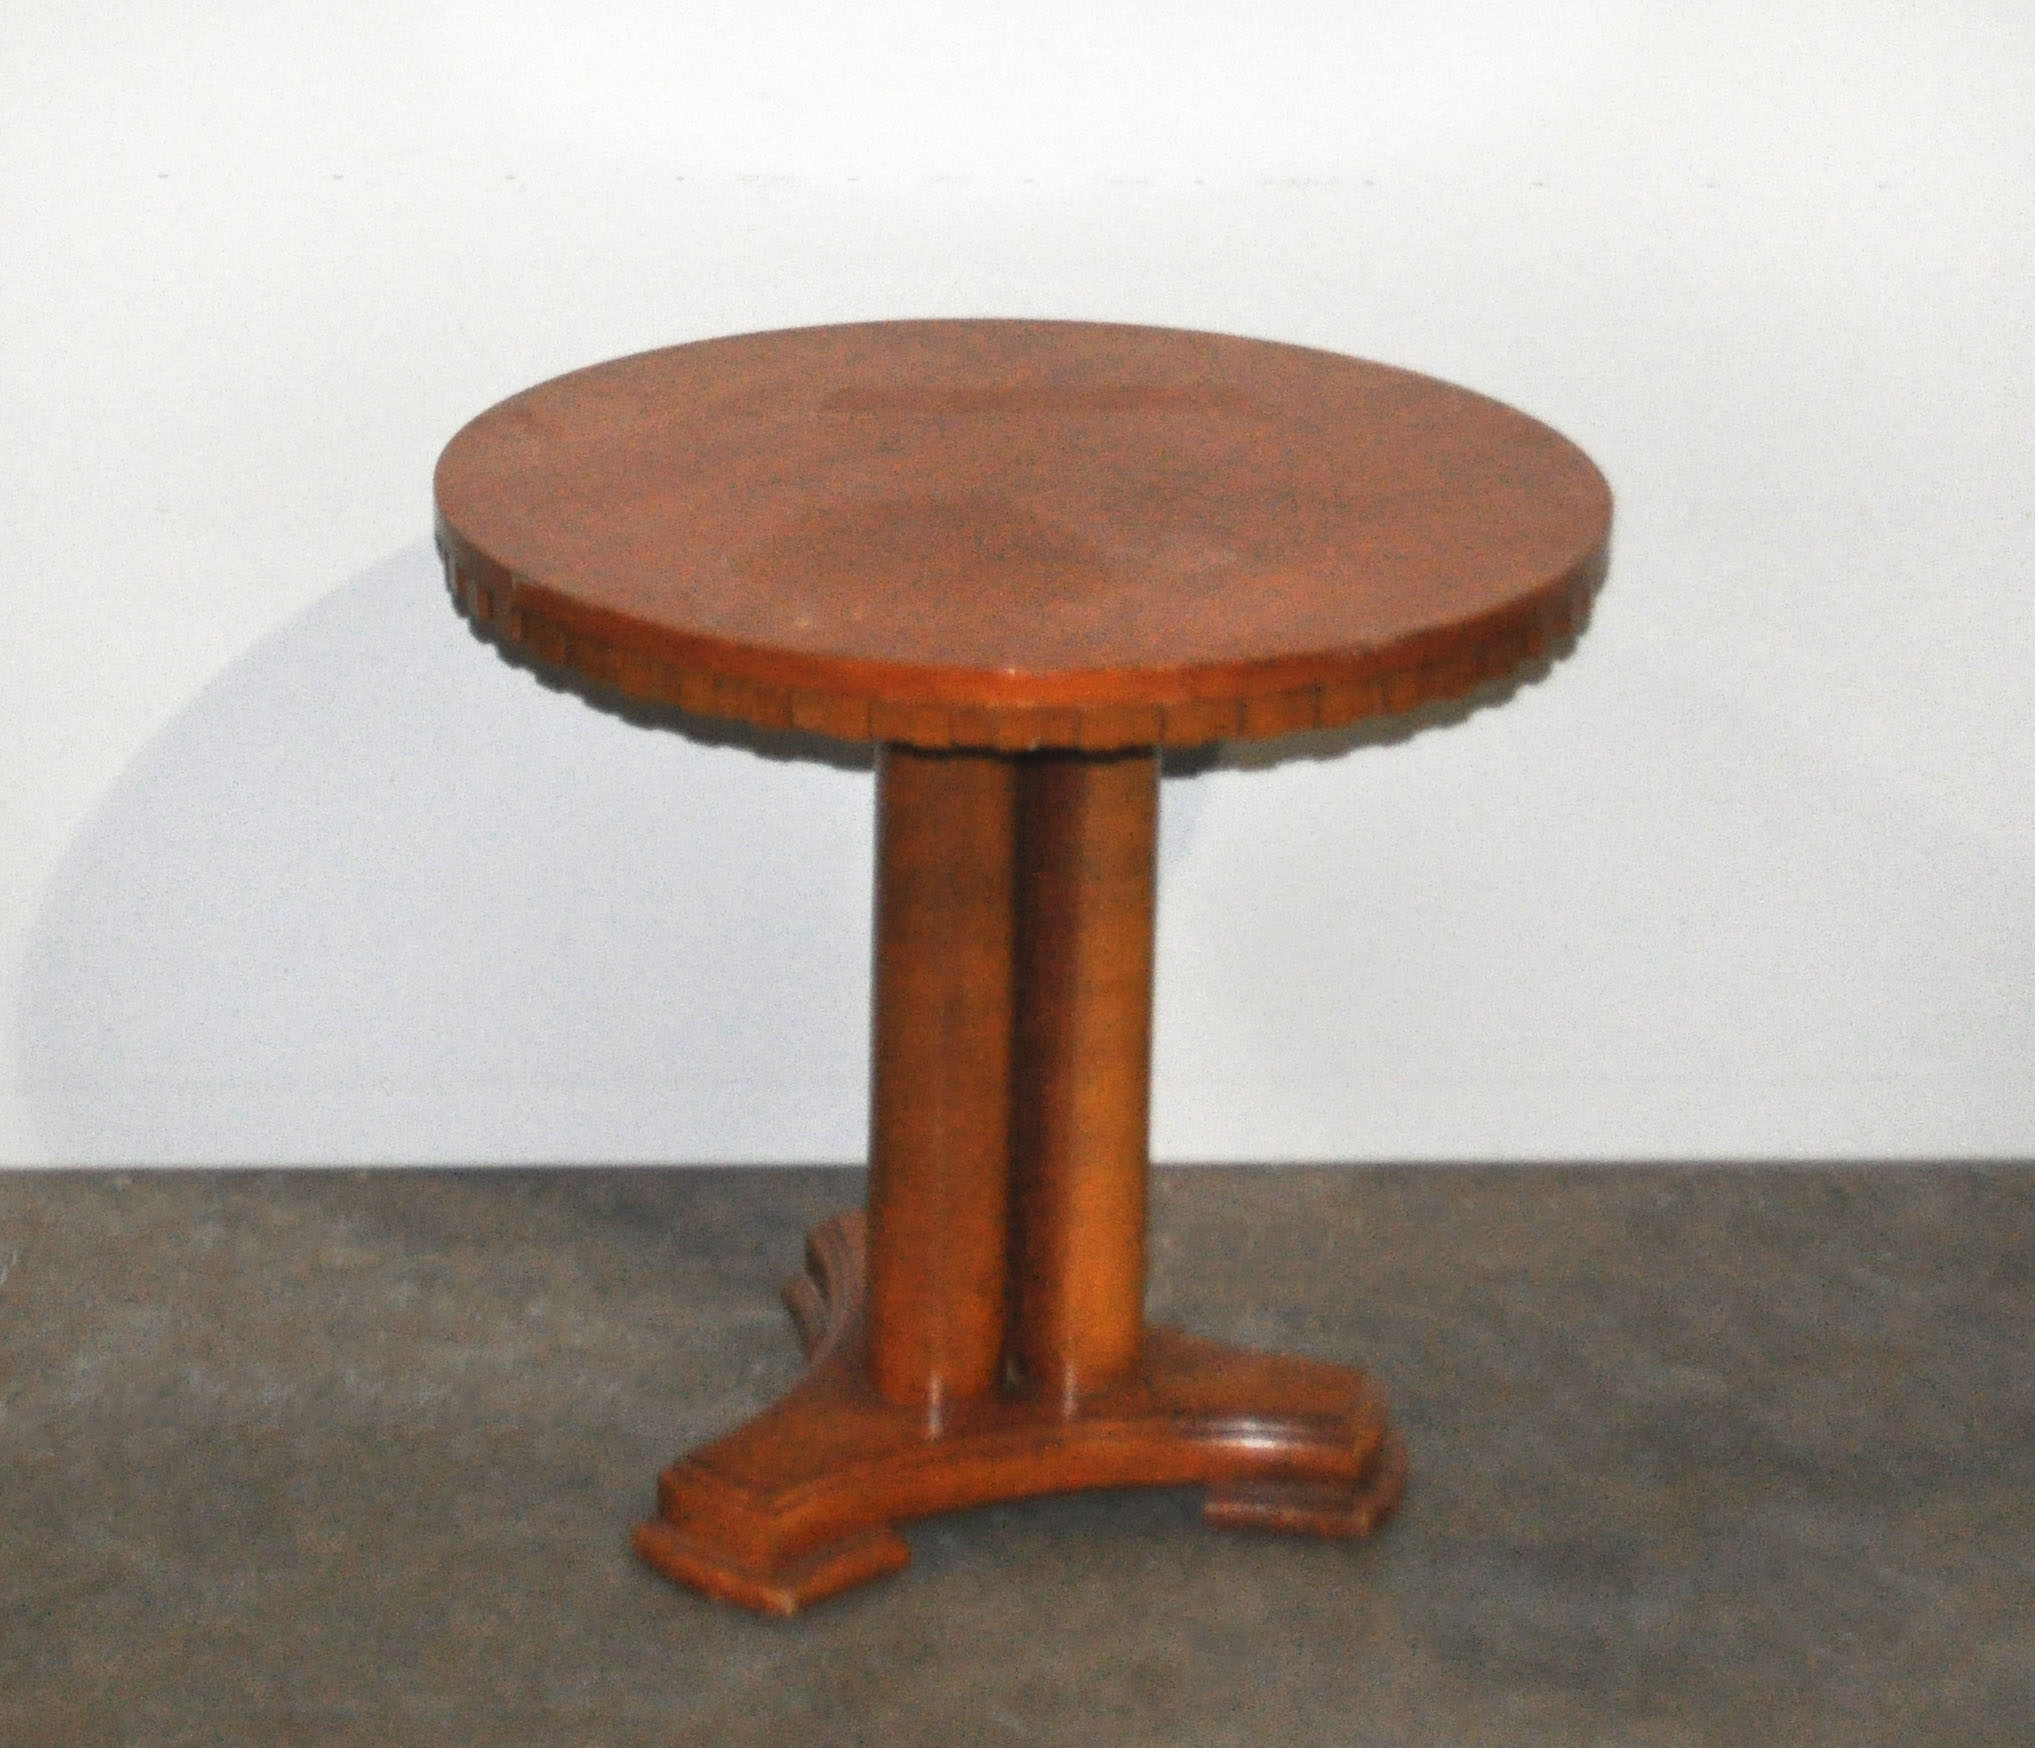
\includegraphics[width=3cm]{0_Images/Furniture/EndTable.jpg}} &
		\subfloat[Coffee Table]{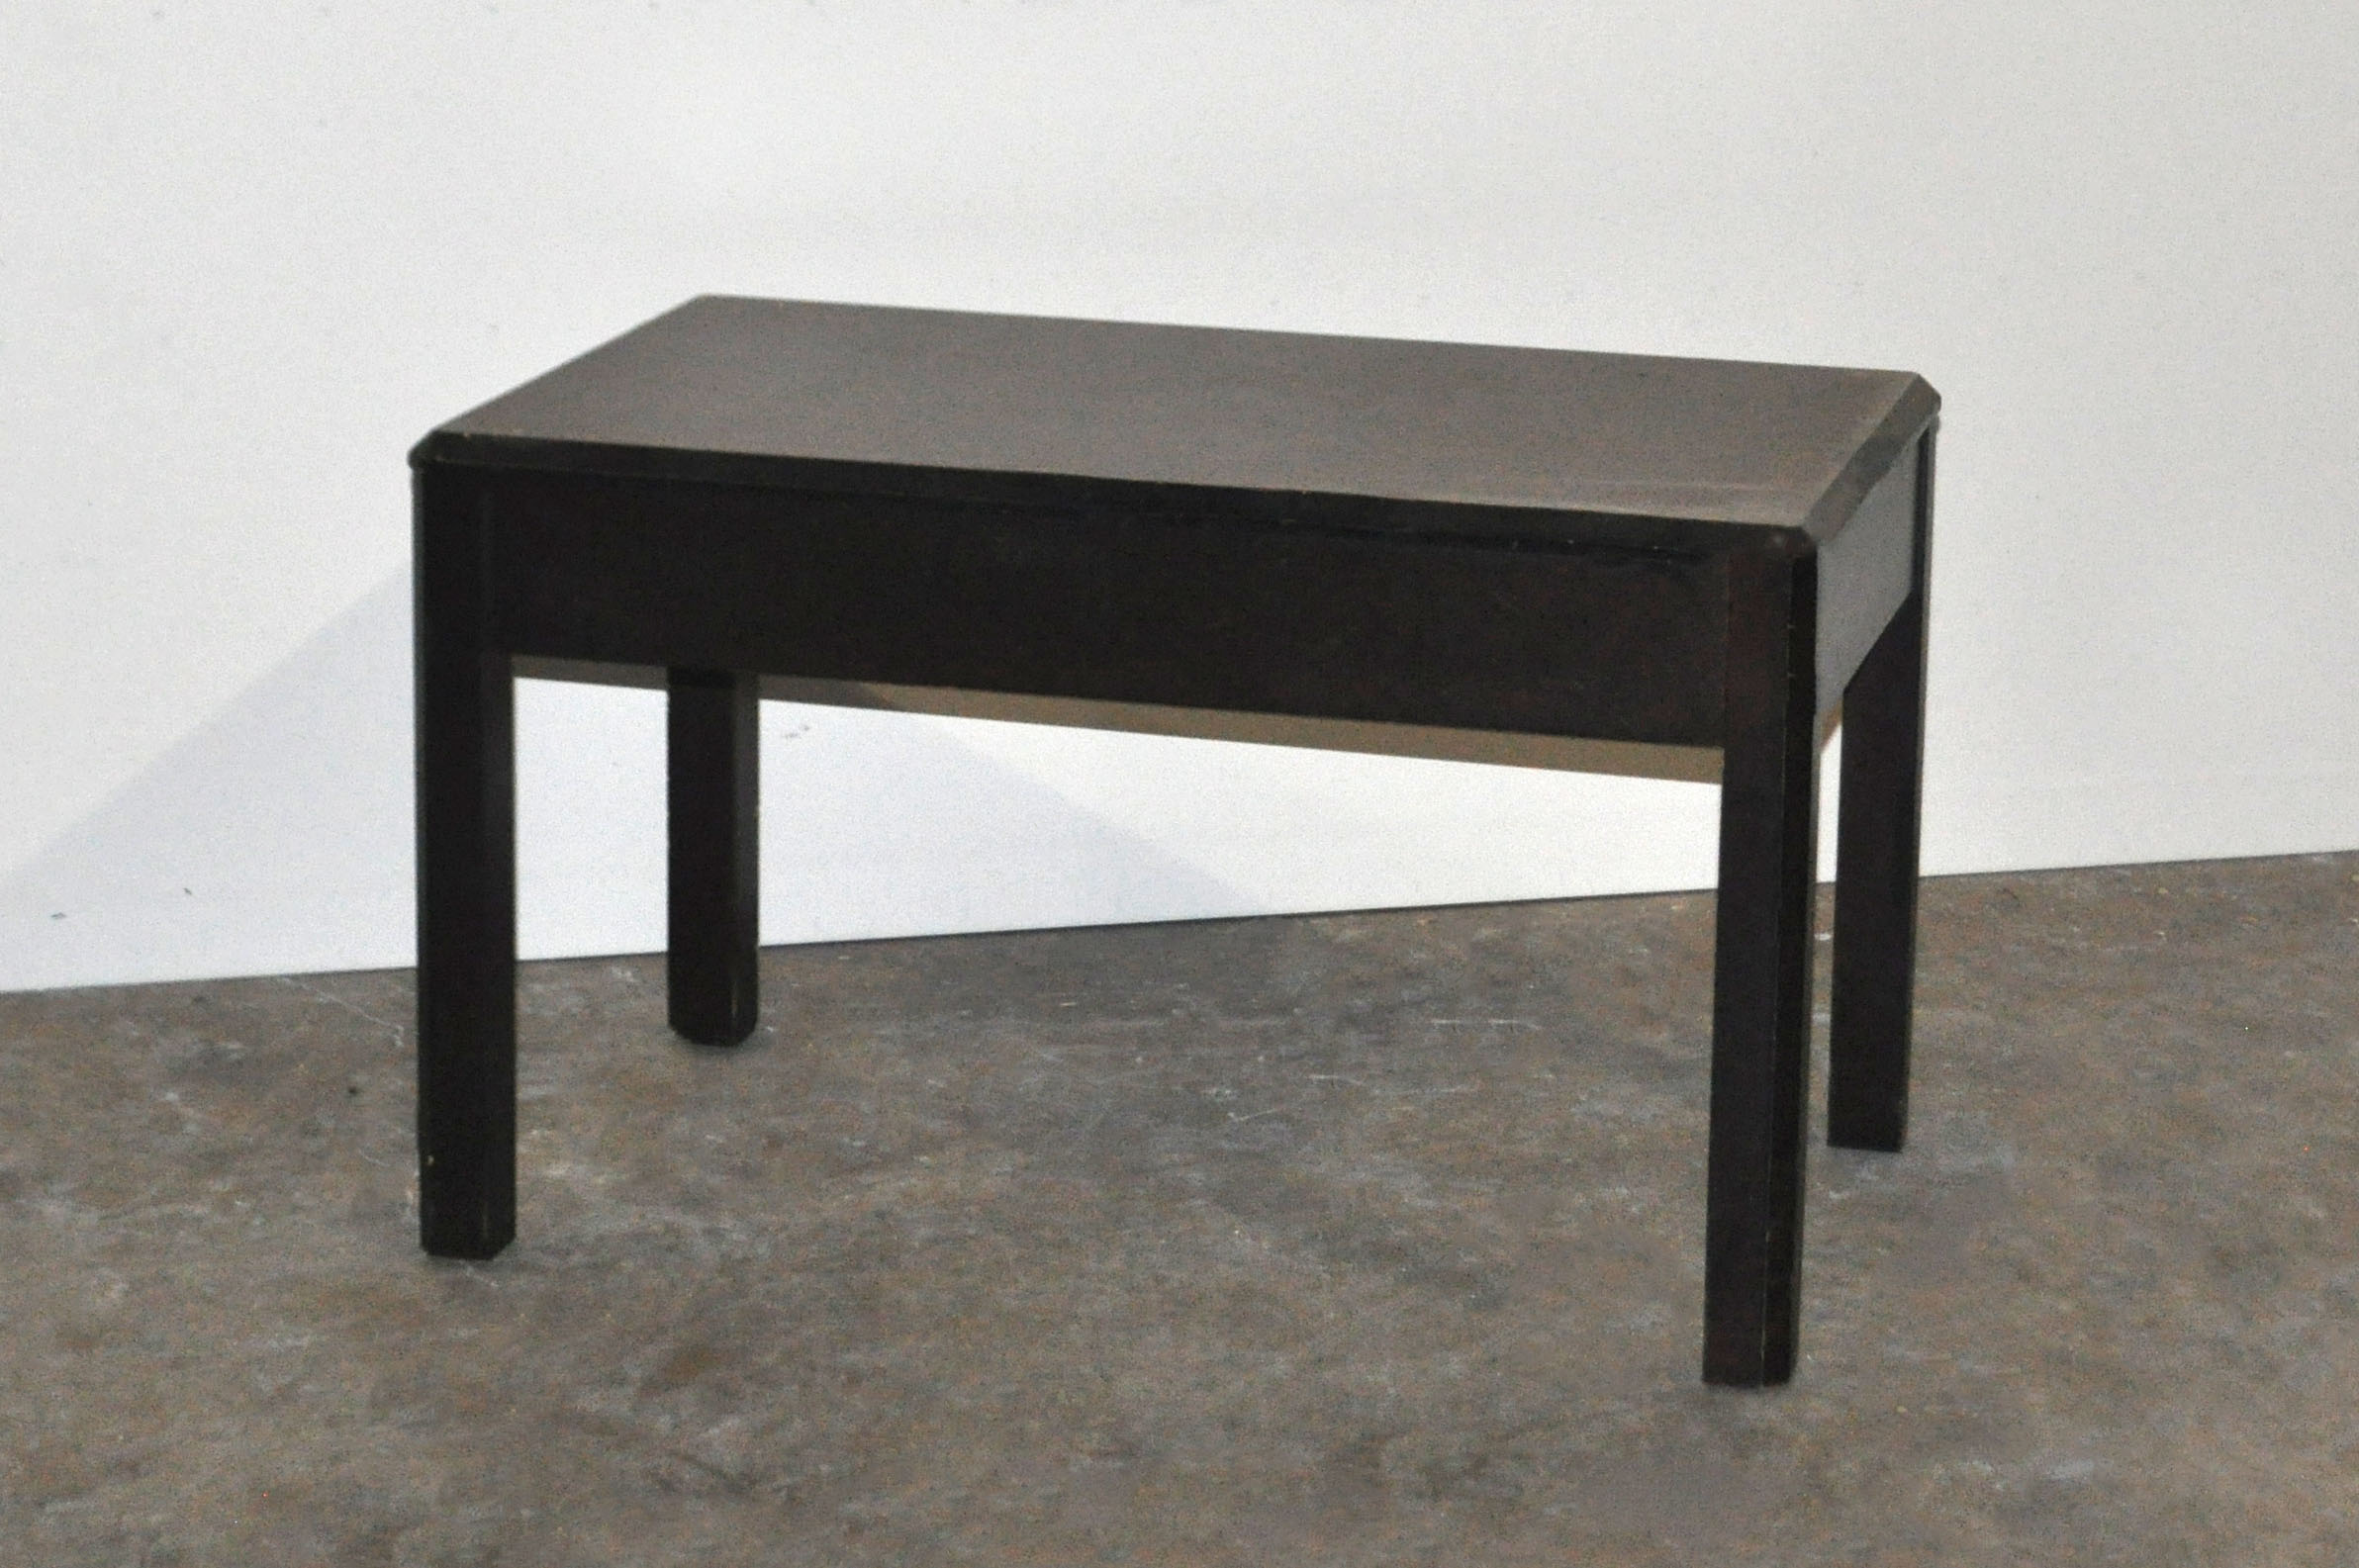
\includegraphics[width=3cm]{0_Images/Furniture/CoffeeTable.jpg}} &
		\subfloat[Lamp]{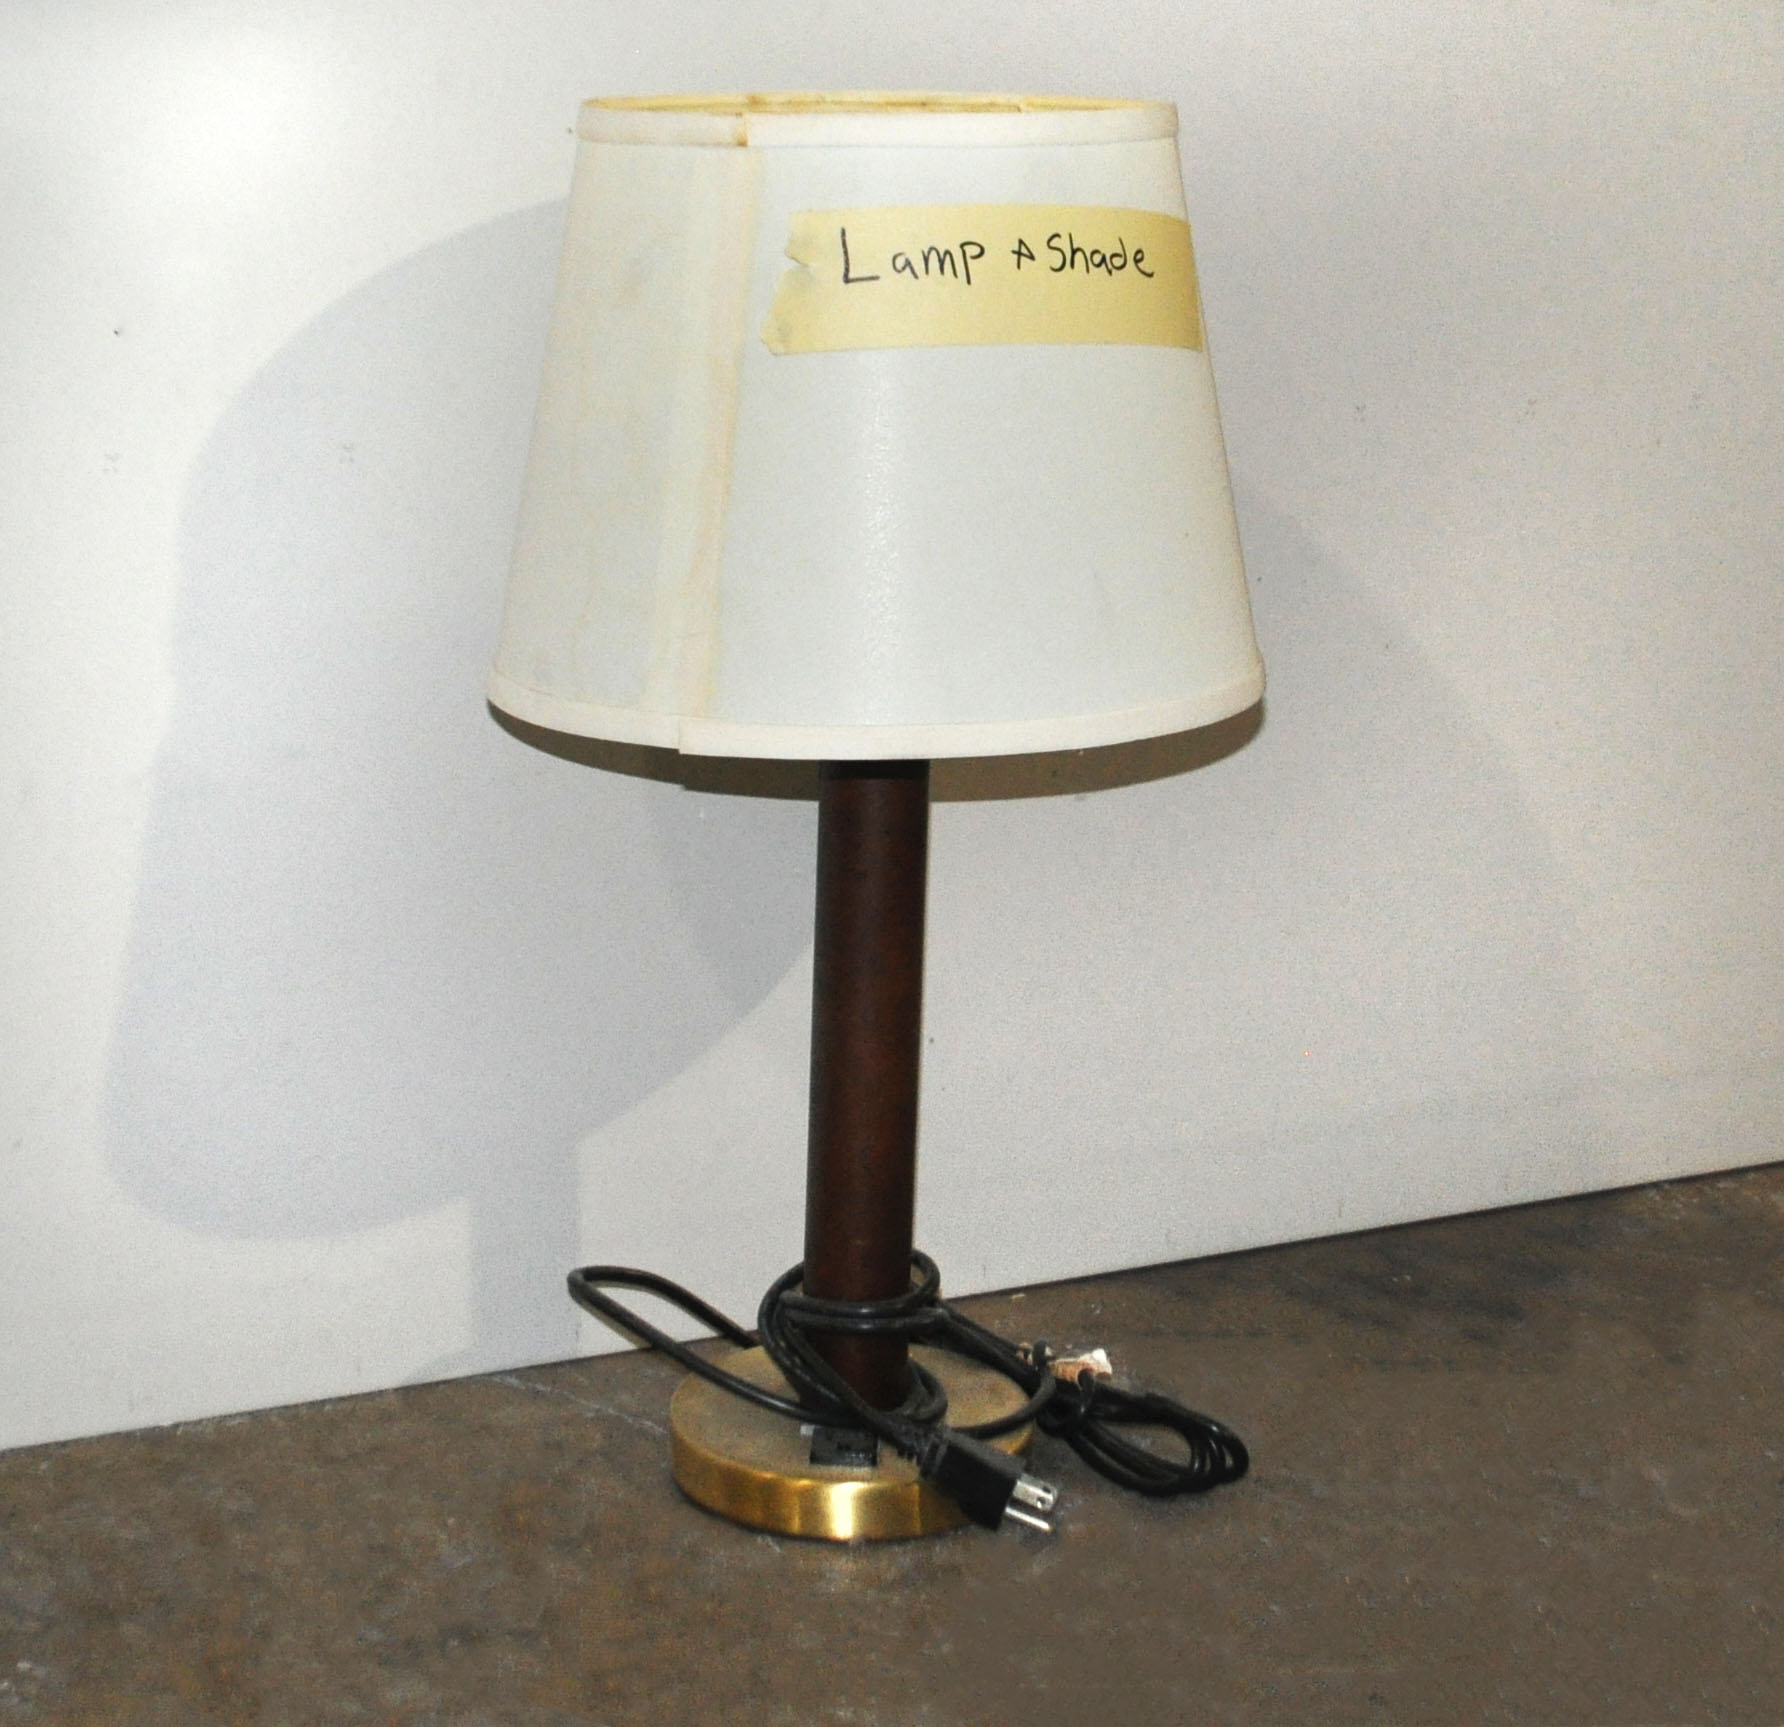
\includegraphics[width=3cm]{0_Images/Furniture/Lamp_and_Shade.jpg}} &
		\subfloat[Chair (Yellow)]{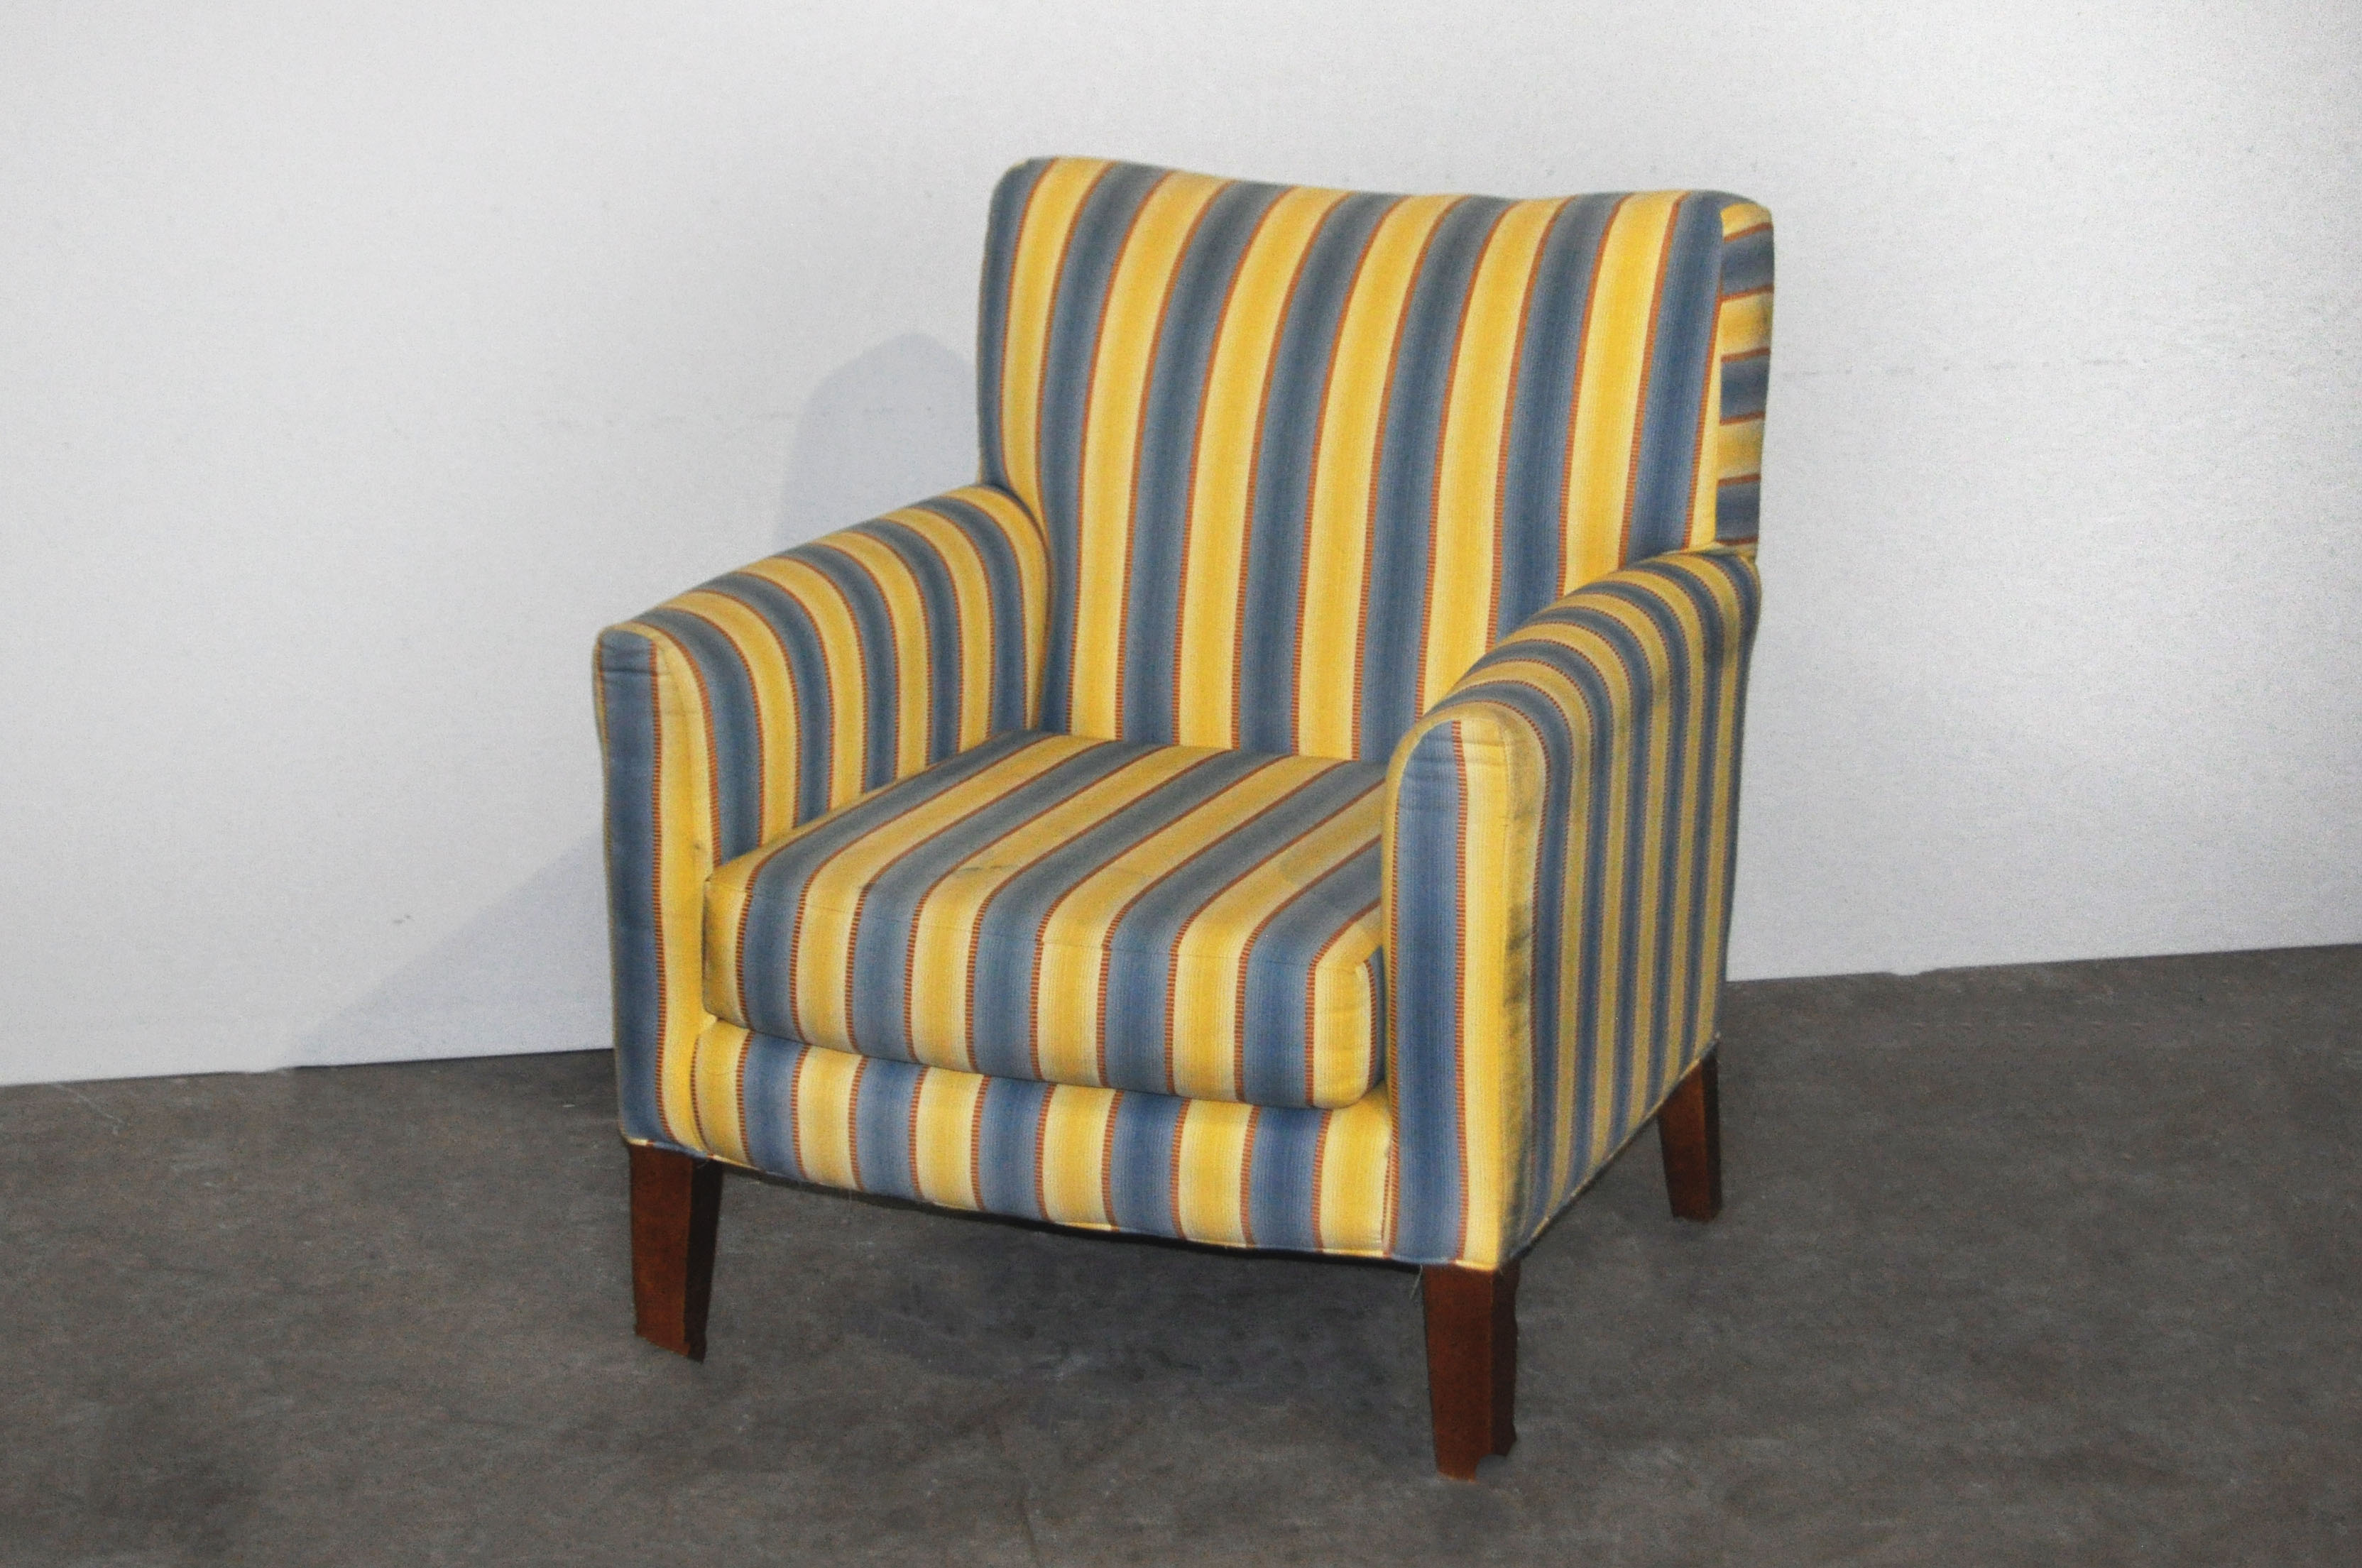
\includegraphics[width=3cm]{0_Images/Furniture/Chair(Yellow).jpg}} \\
		\subfloat[Chair (Brown)]{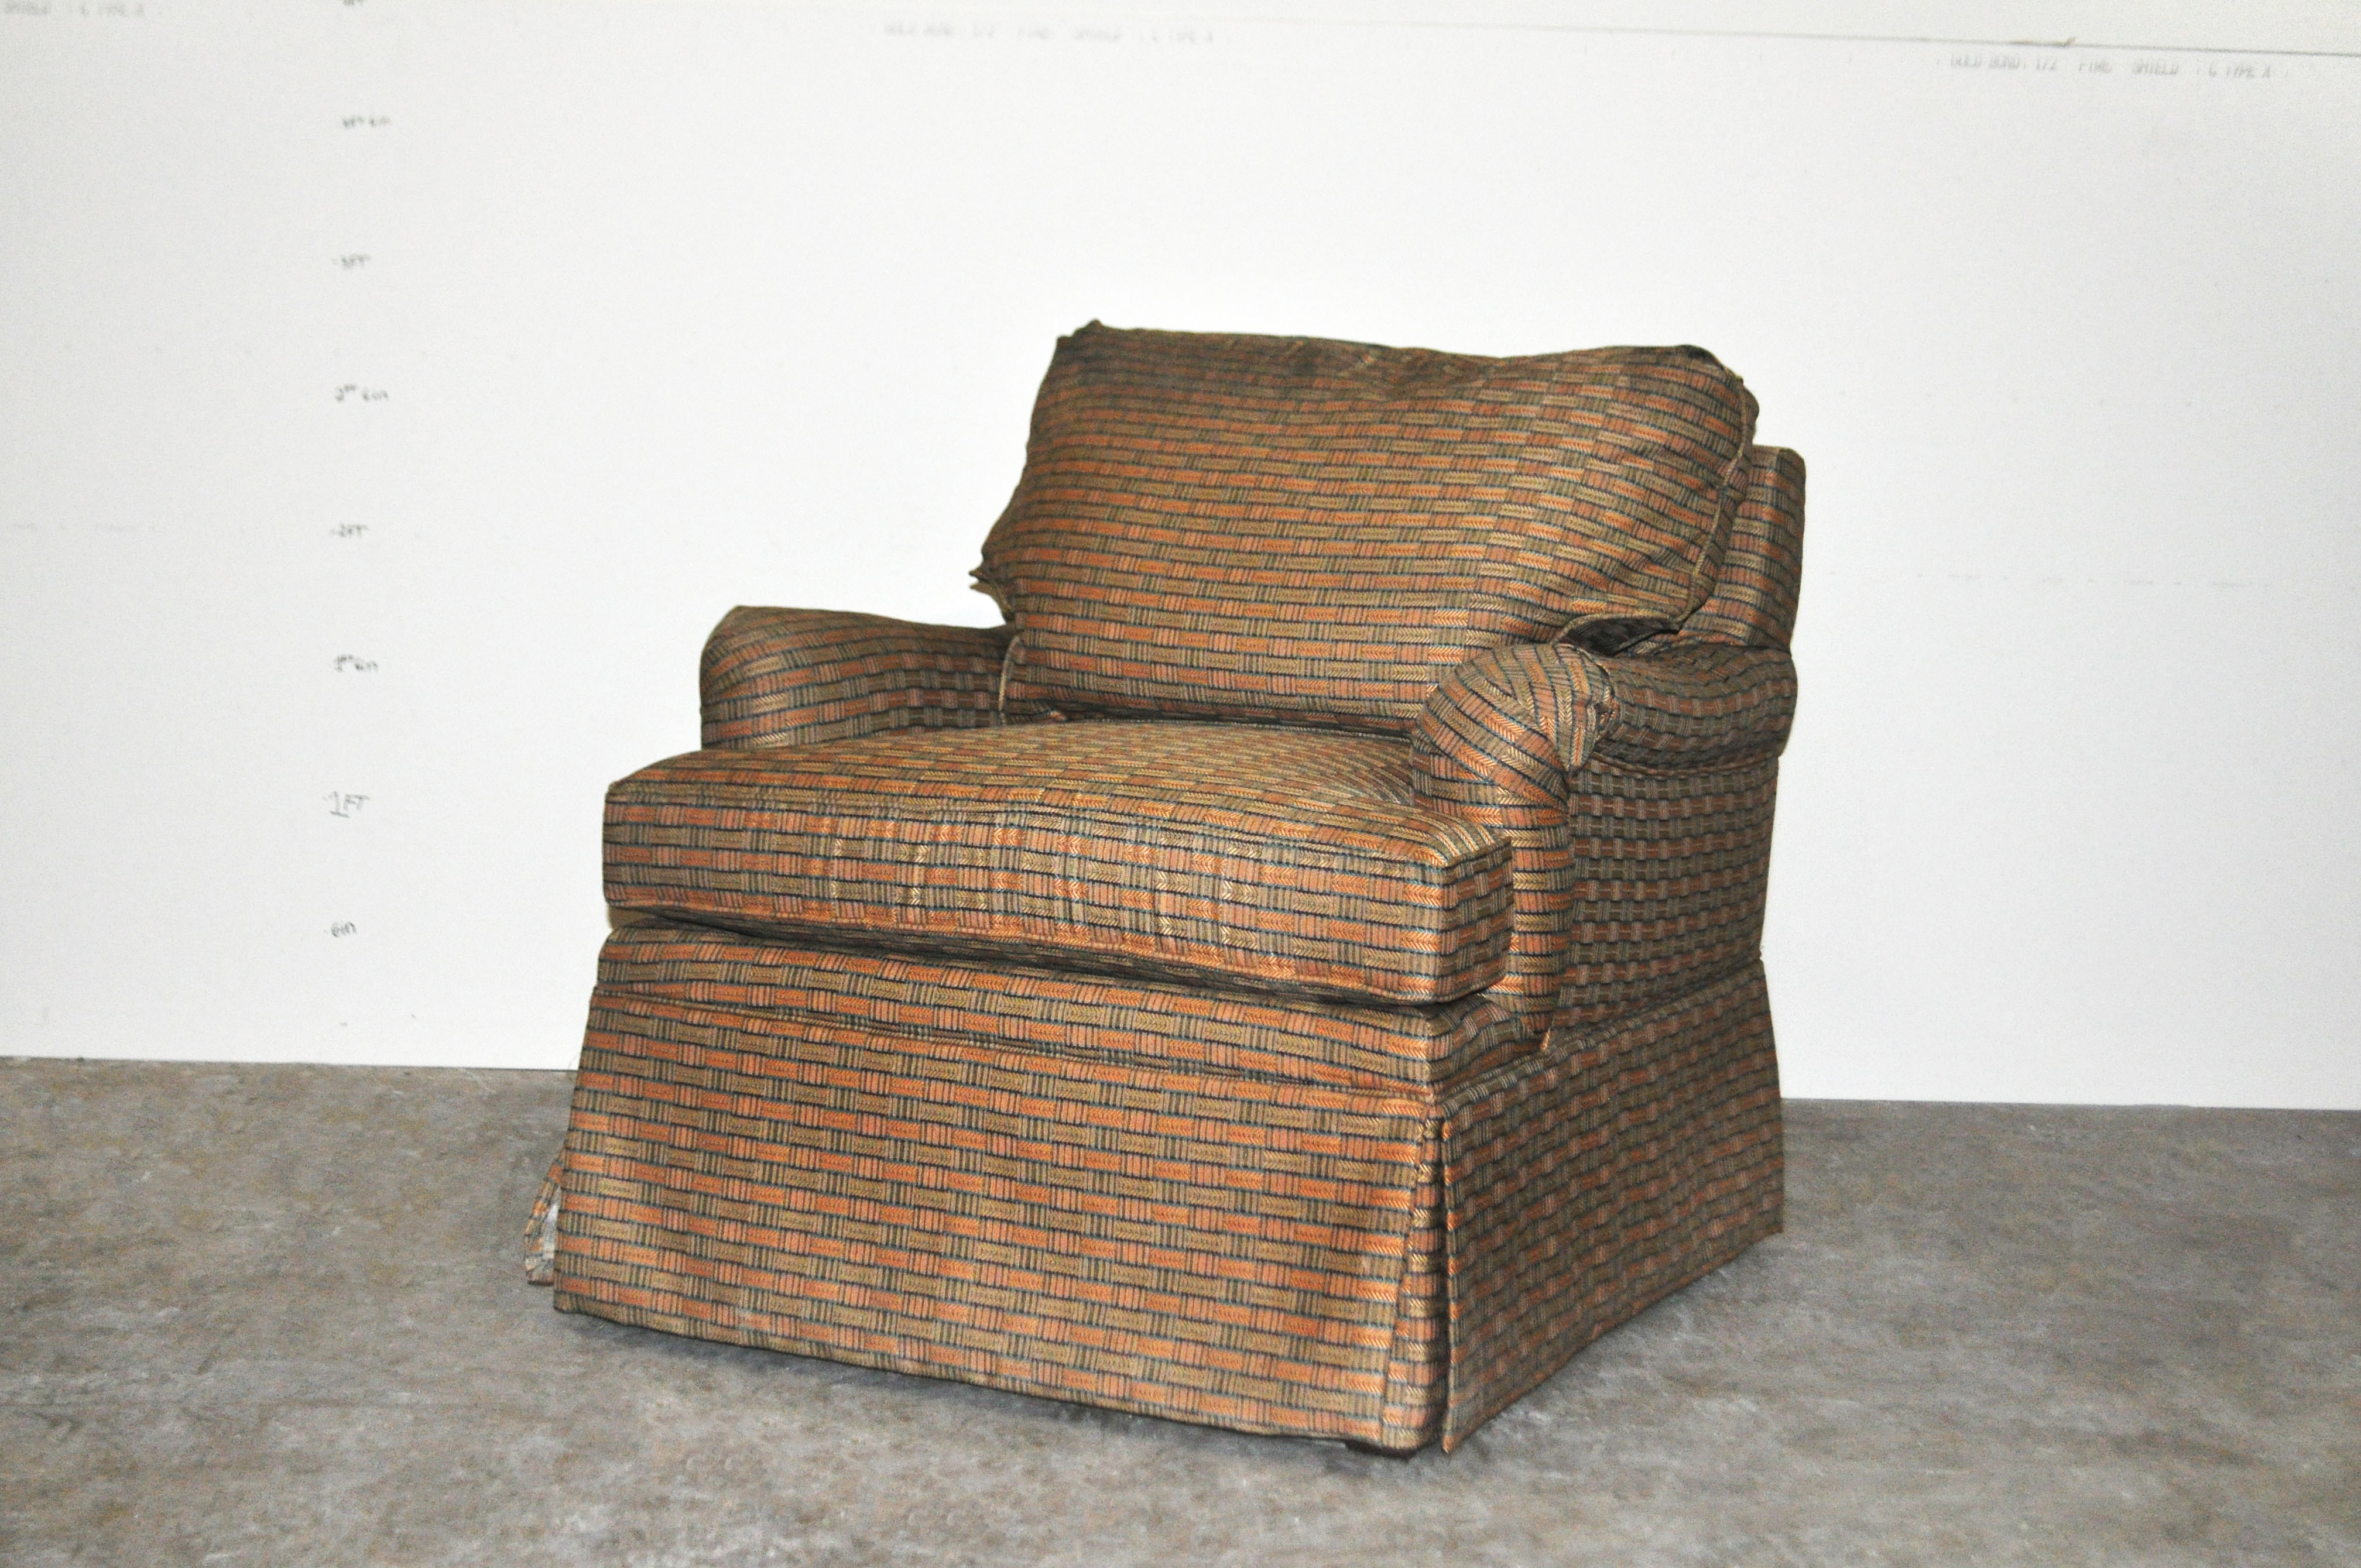
\includegraphics[width=3cm]{0_Images/Furniture/Chair(Brown).jpg}} &
		\subfloat[Sofa (Green)]{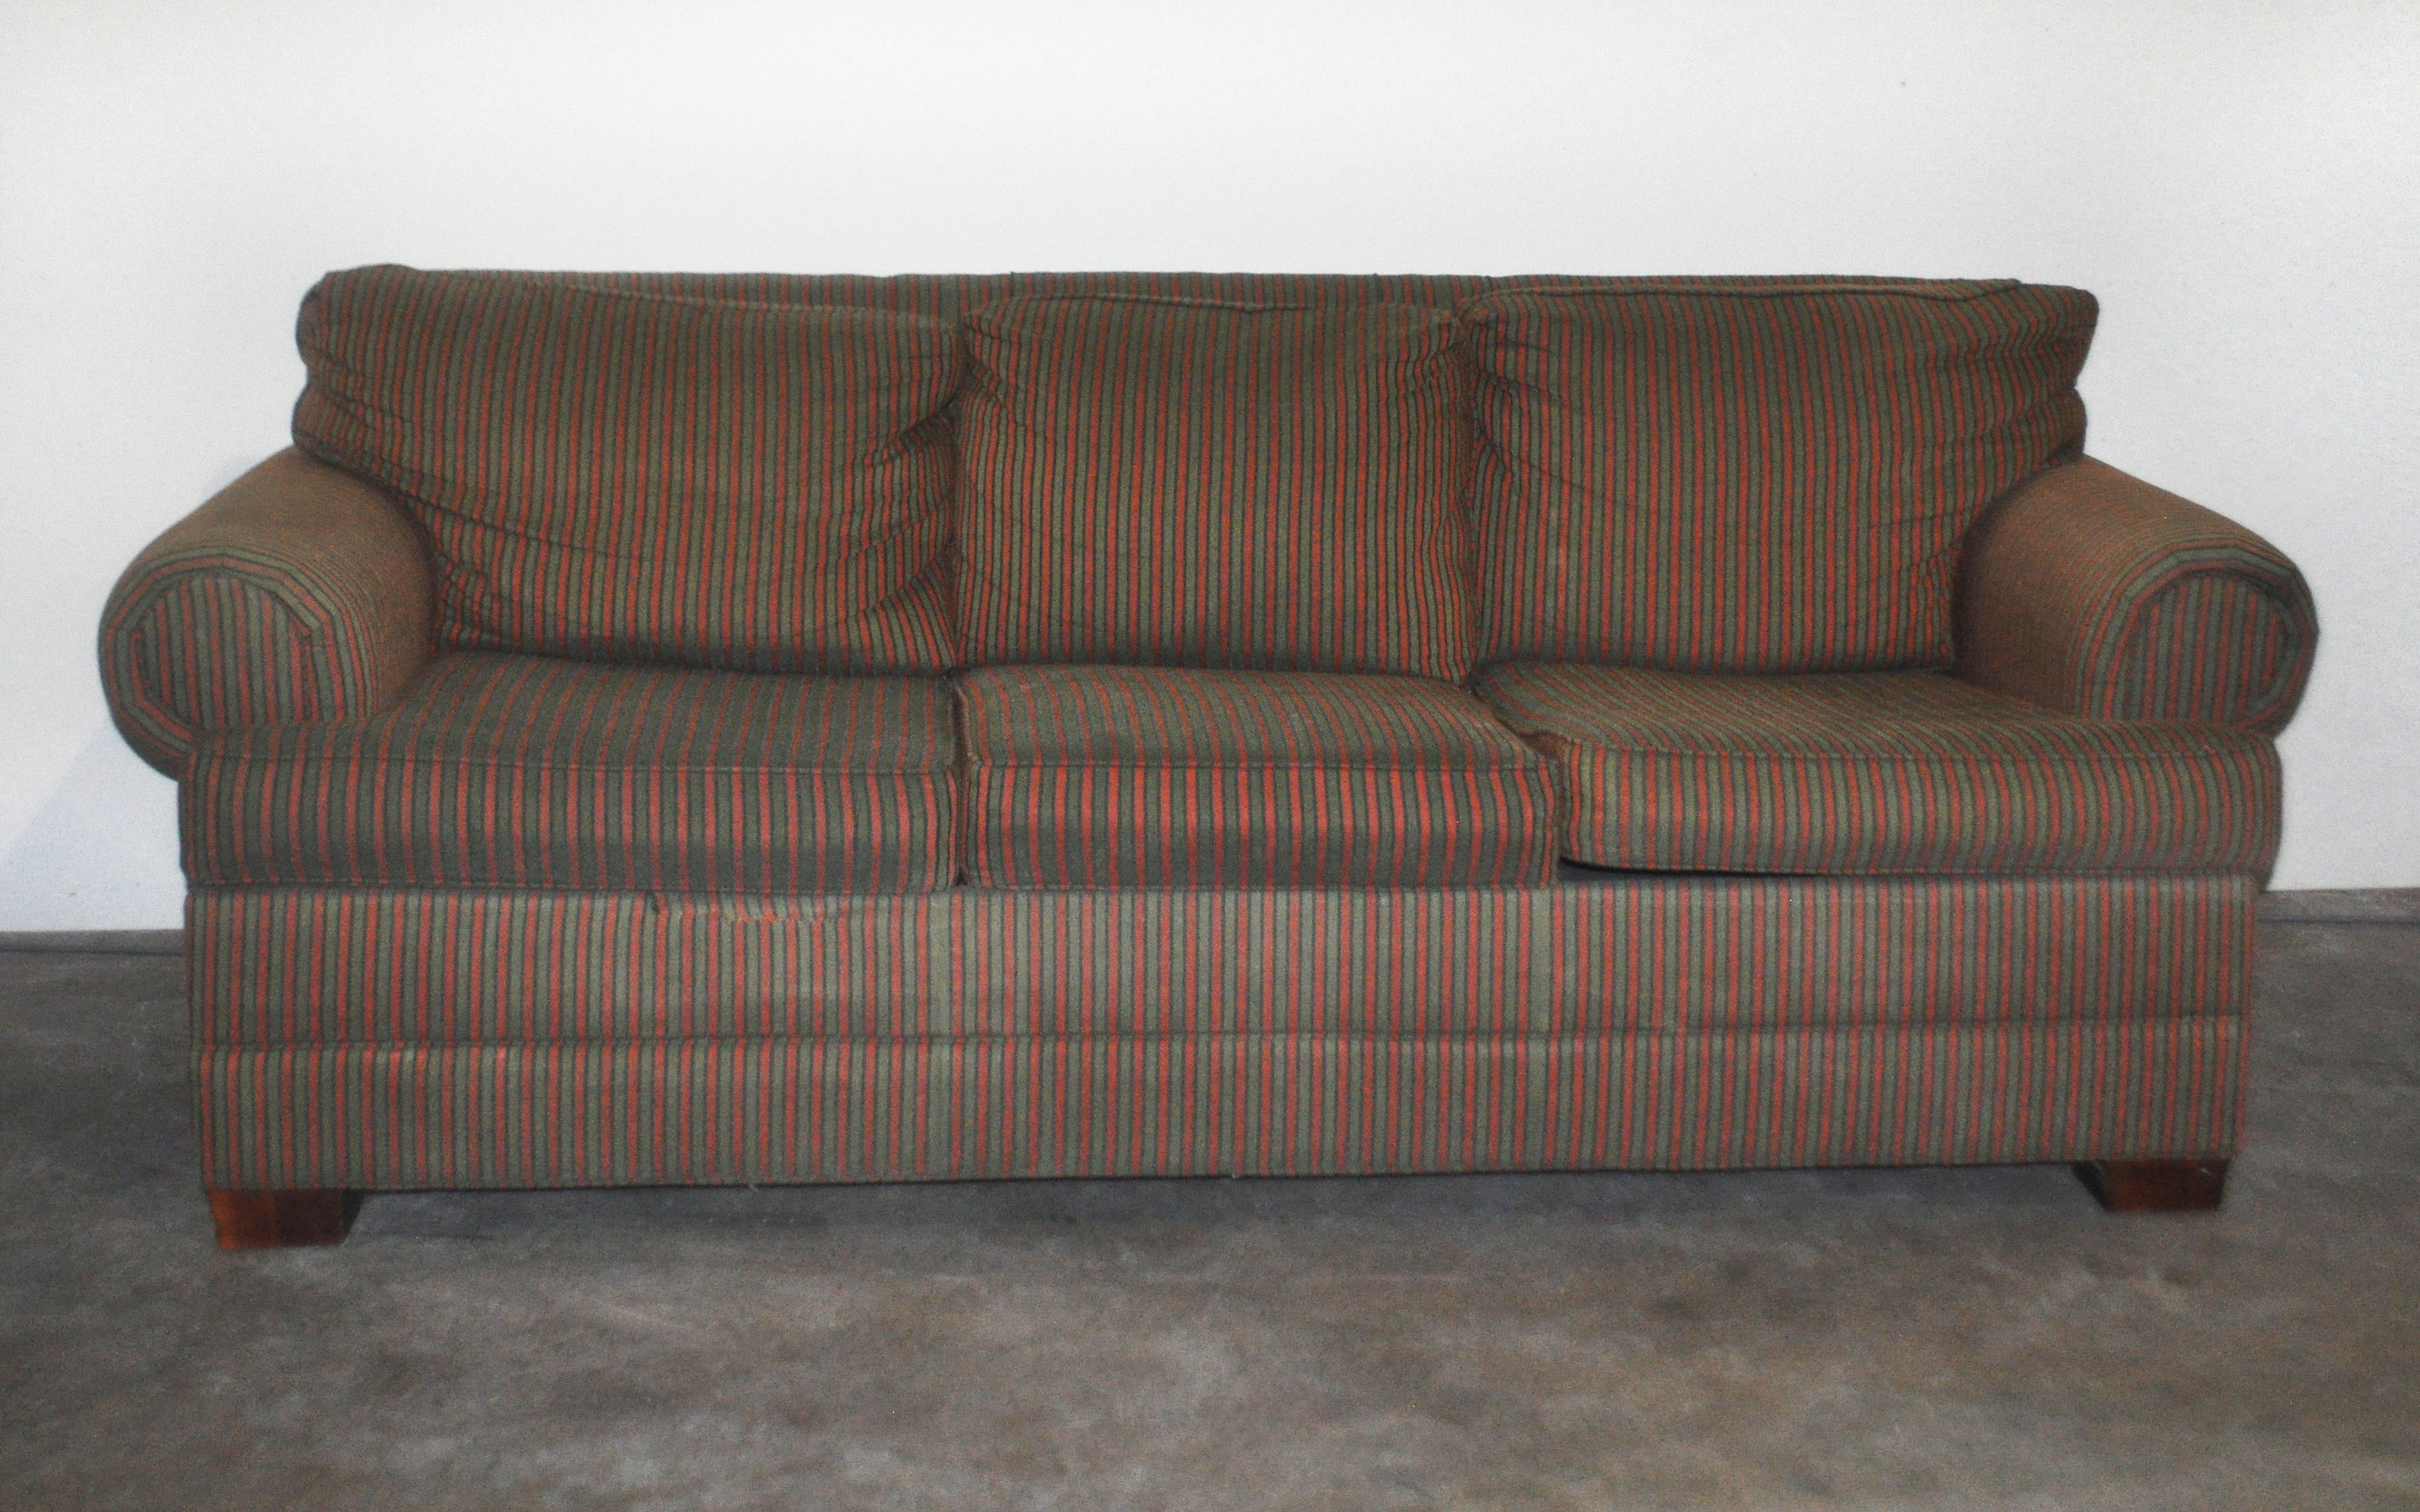
\includegraphics[width=3cm]{0_Images/Furniture/SleeperSofa(Green).jpg}} &
		\subfloat[Sofa (Orange)]{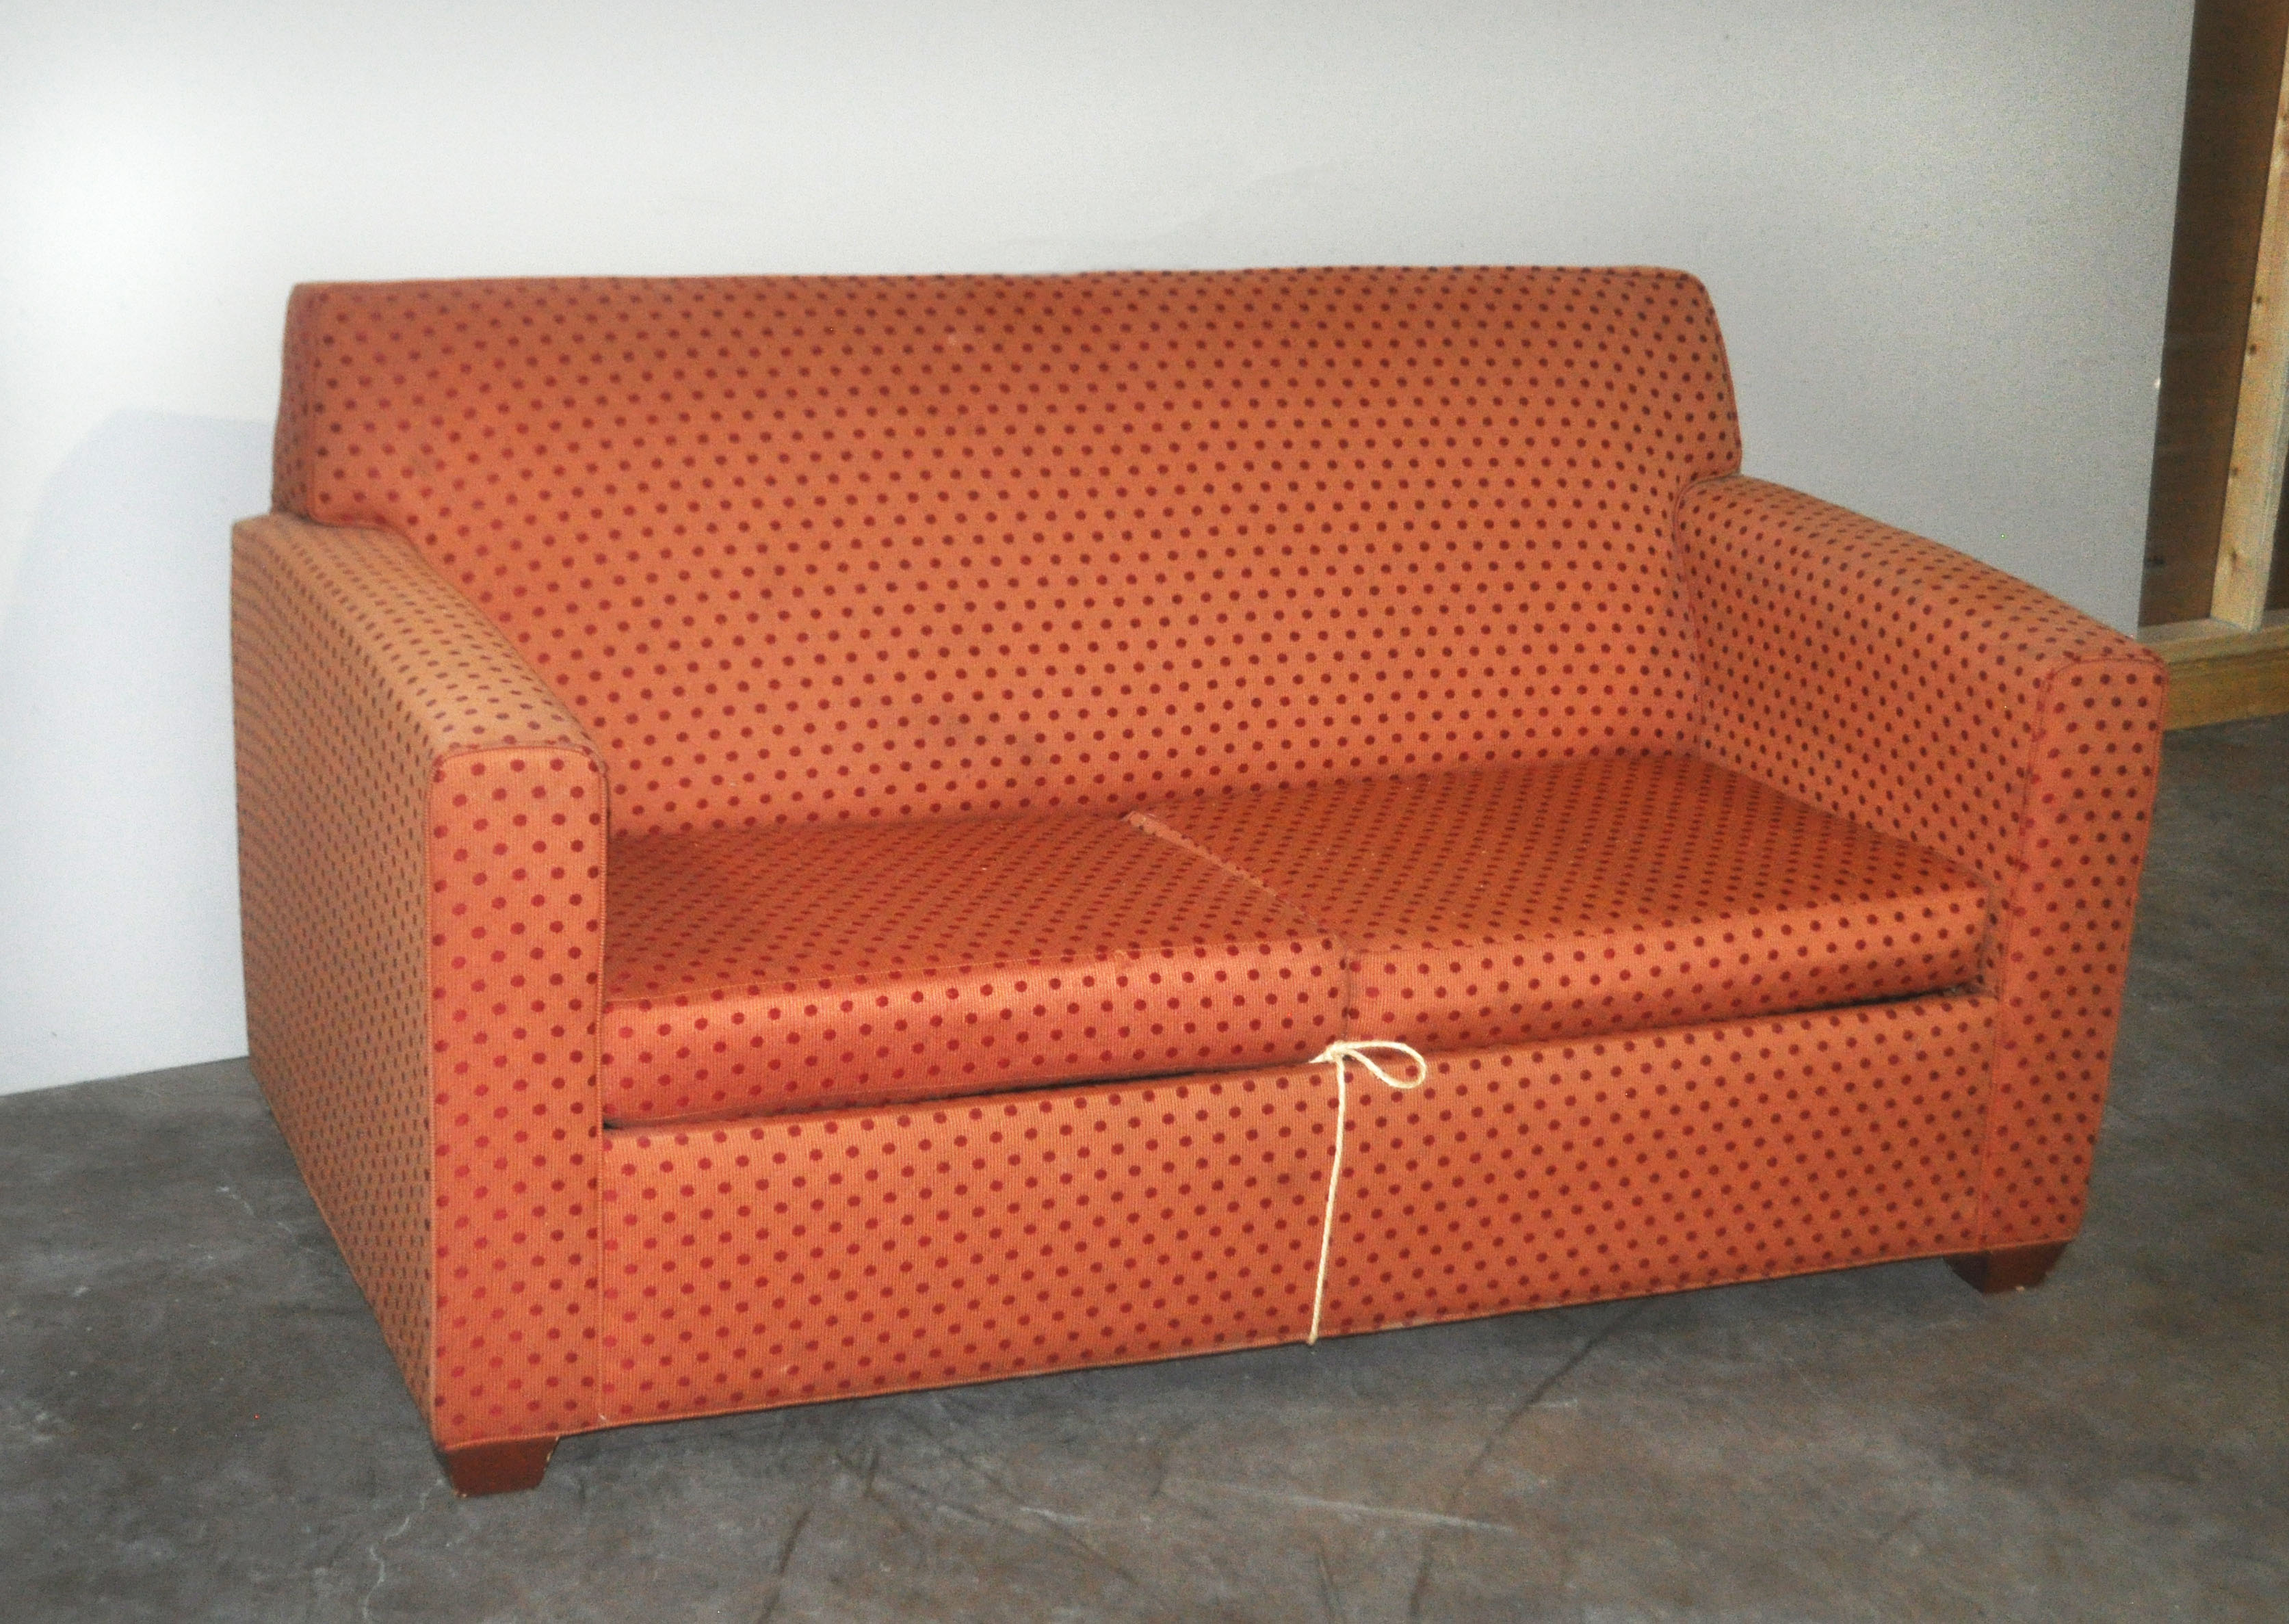
\includegraphics[width=3cm]{0_Images/Furniture/SleeperSofa(Orange).jpg}} &
		\subfloat[Curtain]{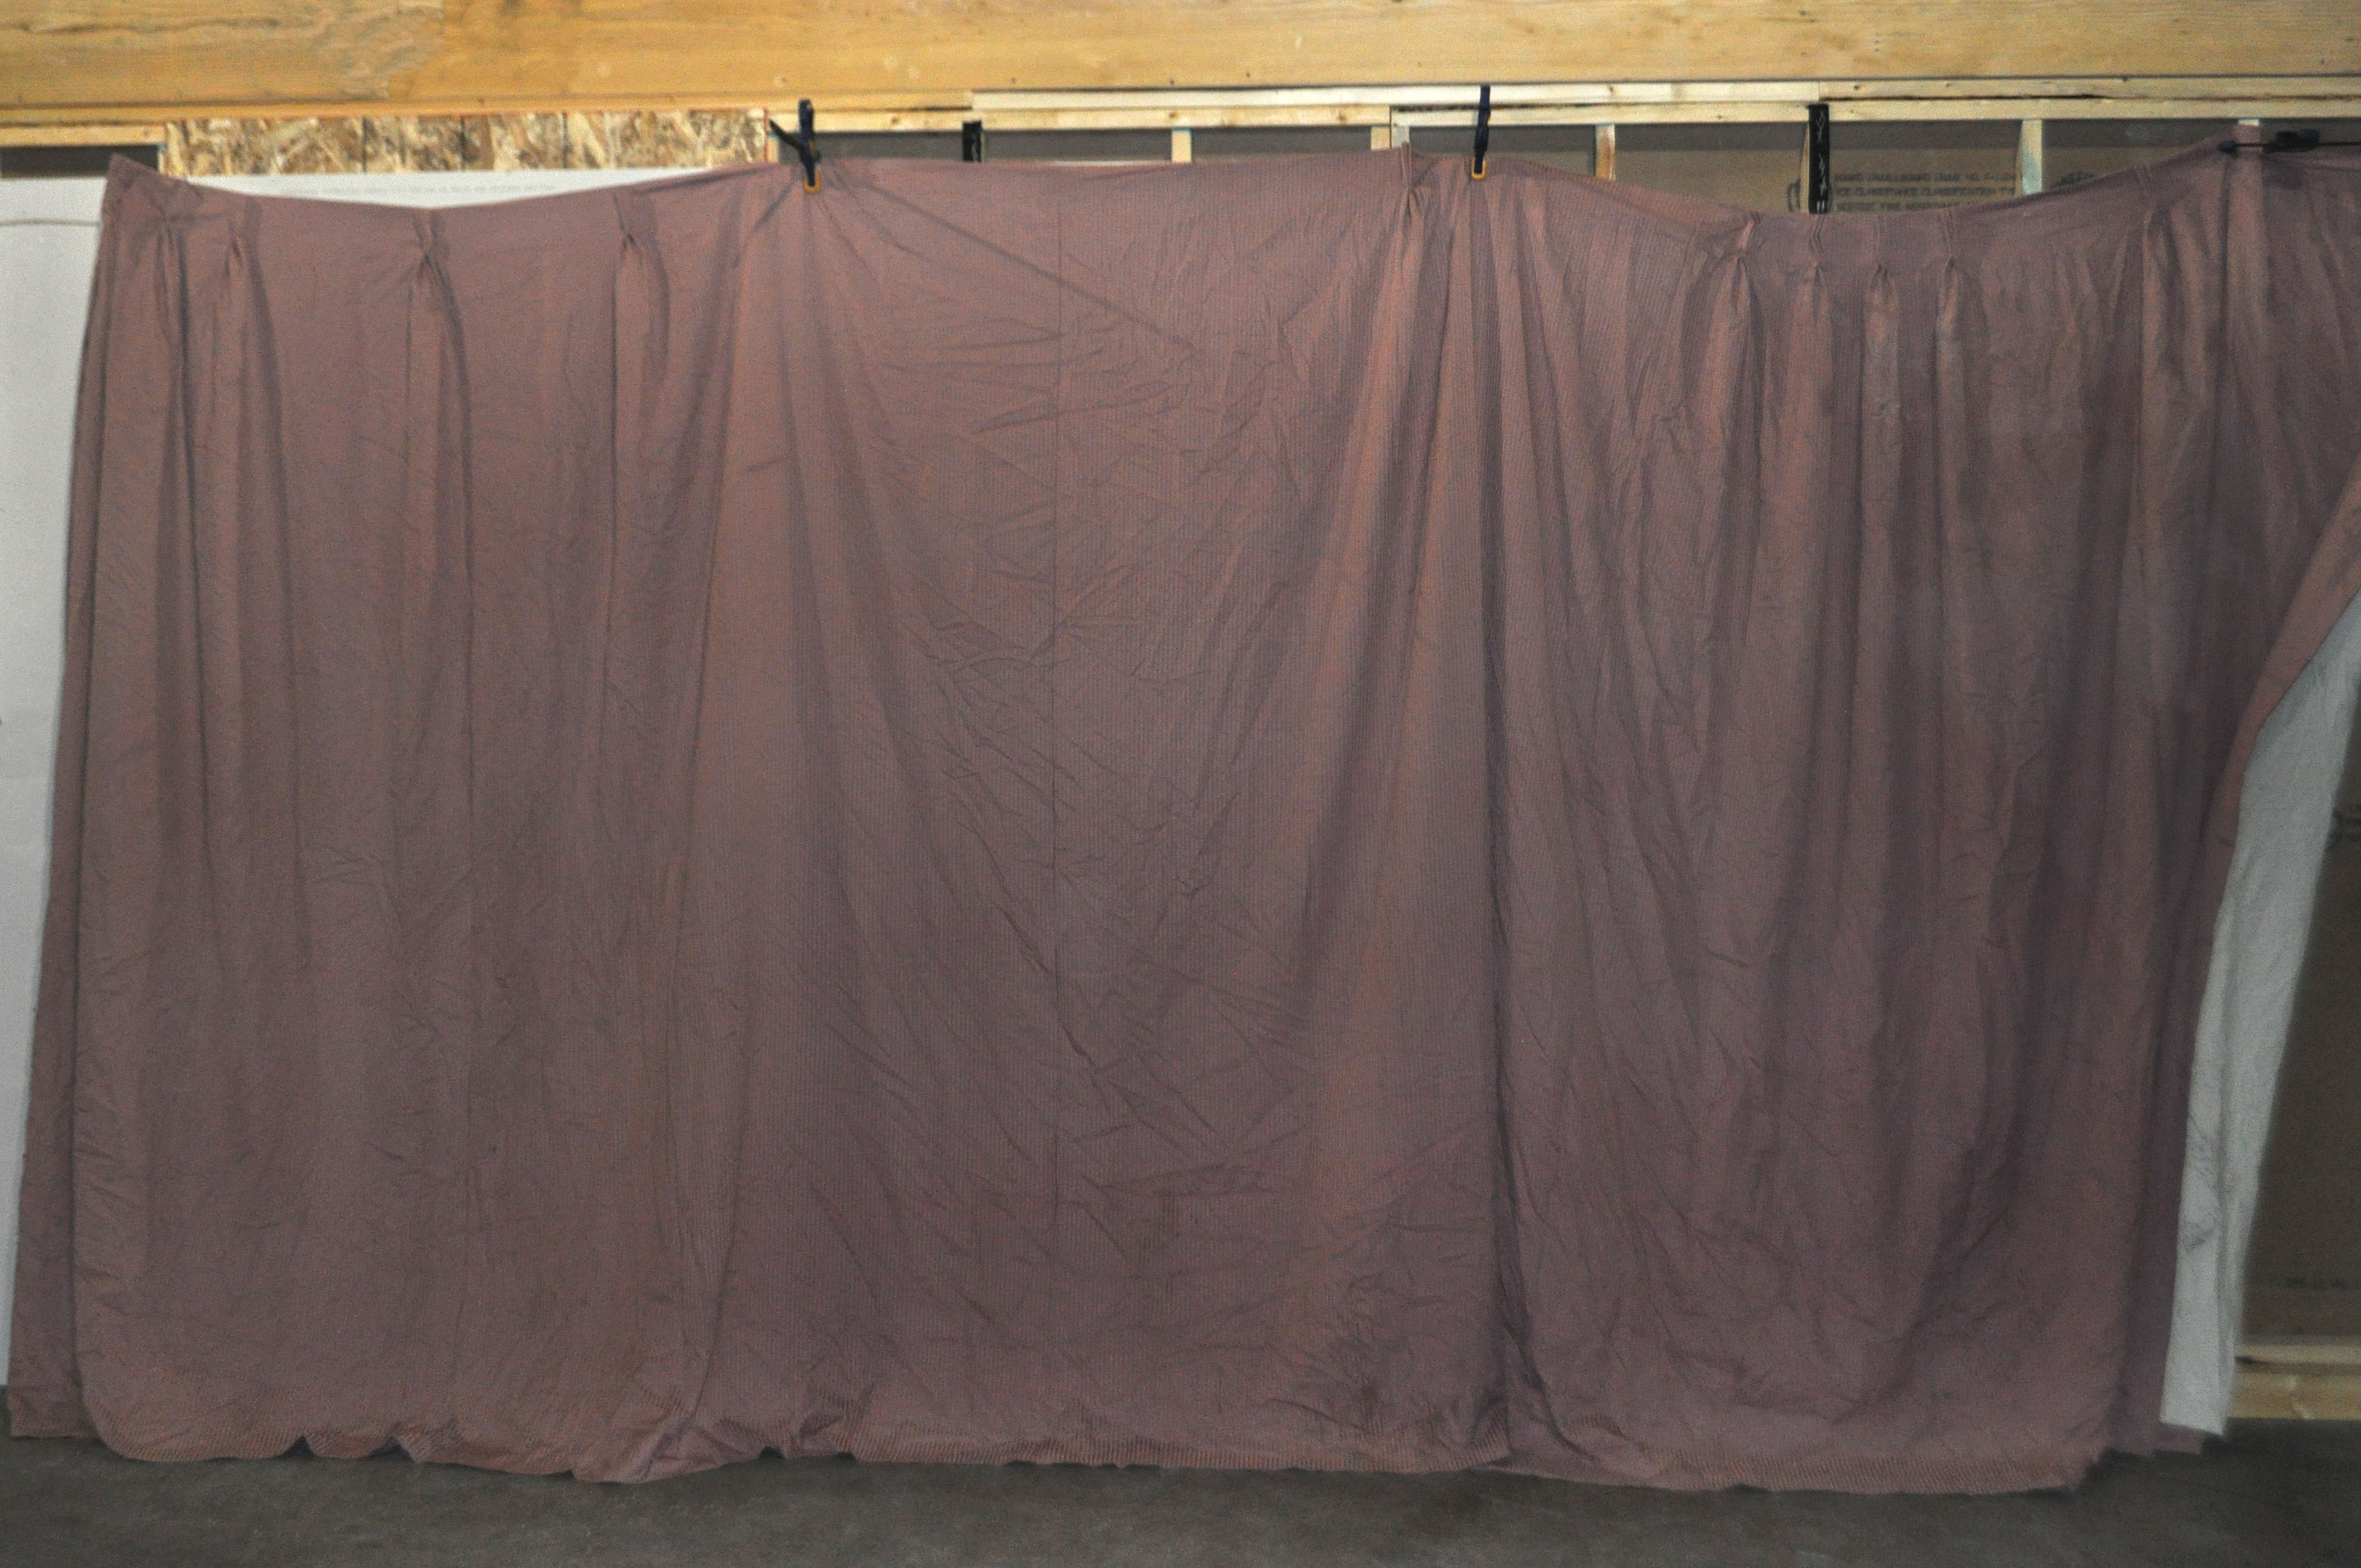
\includegraphics[width=3cm]{0_Images/Furniture/Curtian.jpg}} \\
	\end{tabular}
	\caption{Furniture Images}
	\label{fig:FurnitureImages}
\end{figure}

The living room in the one-story house, as well as the family room and the living room in the two-story house, was furnished similarly with two sofas, armoire, television, television stand, ottoman, end table, coffee table, chair, two pictures, lamp with shade and two curtains .  The floor was covered with polyurethane foam padding and polyester carpet. Figure \ref{fig:Living_Family} shows both the single story living room and two story family room furniture setup.  

\begin{figure}[H]
	\centering
	\begin{tabular}[c]{c c}
		\subfloat[Single Story Living Room]{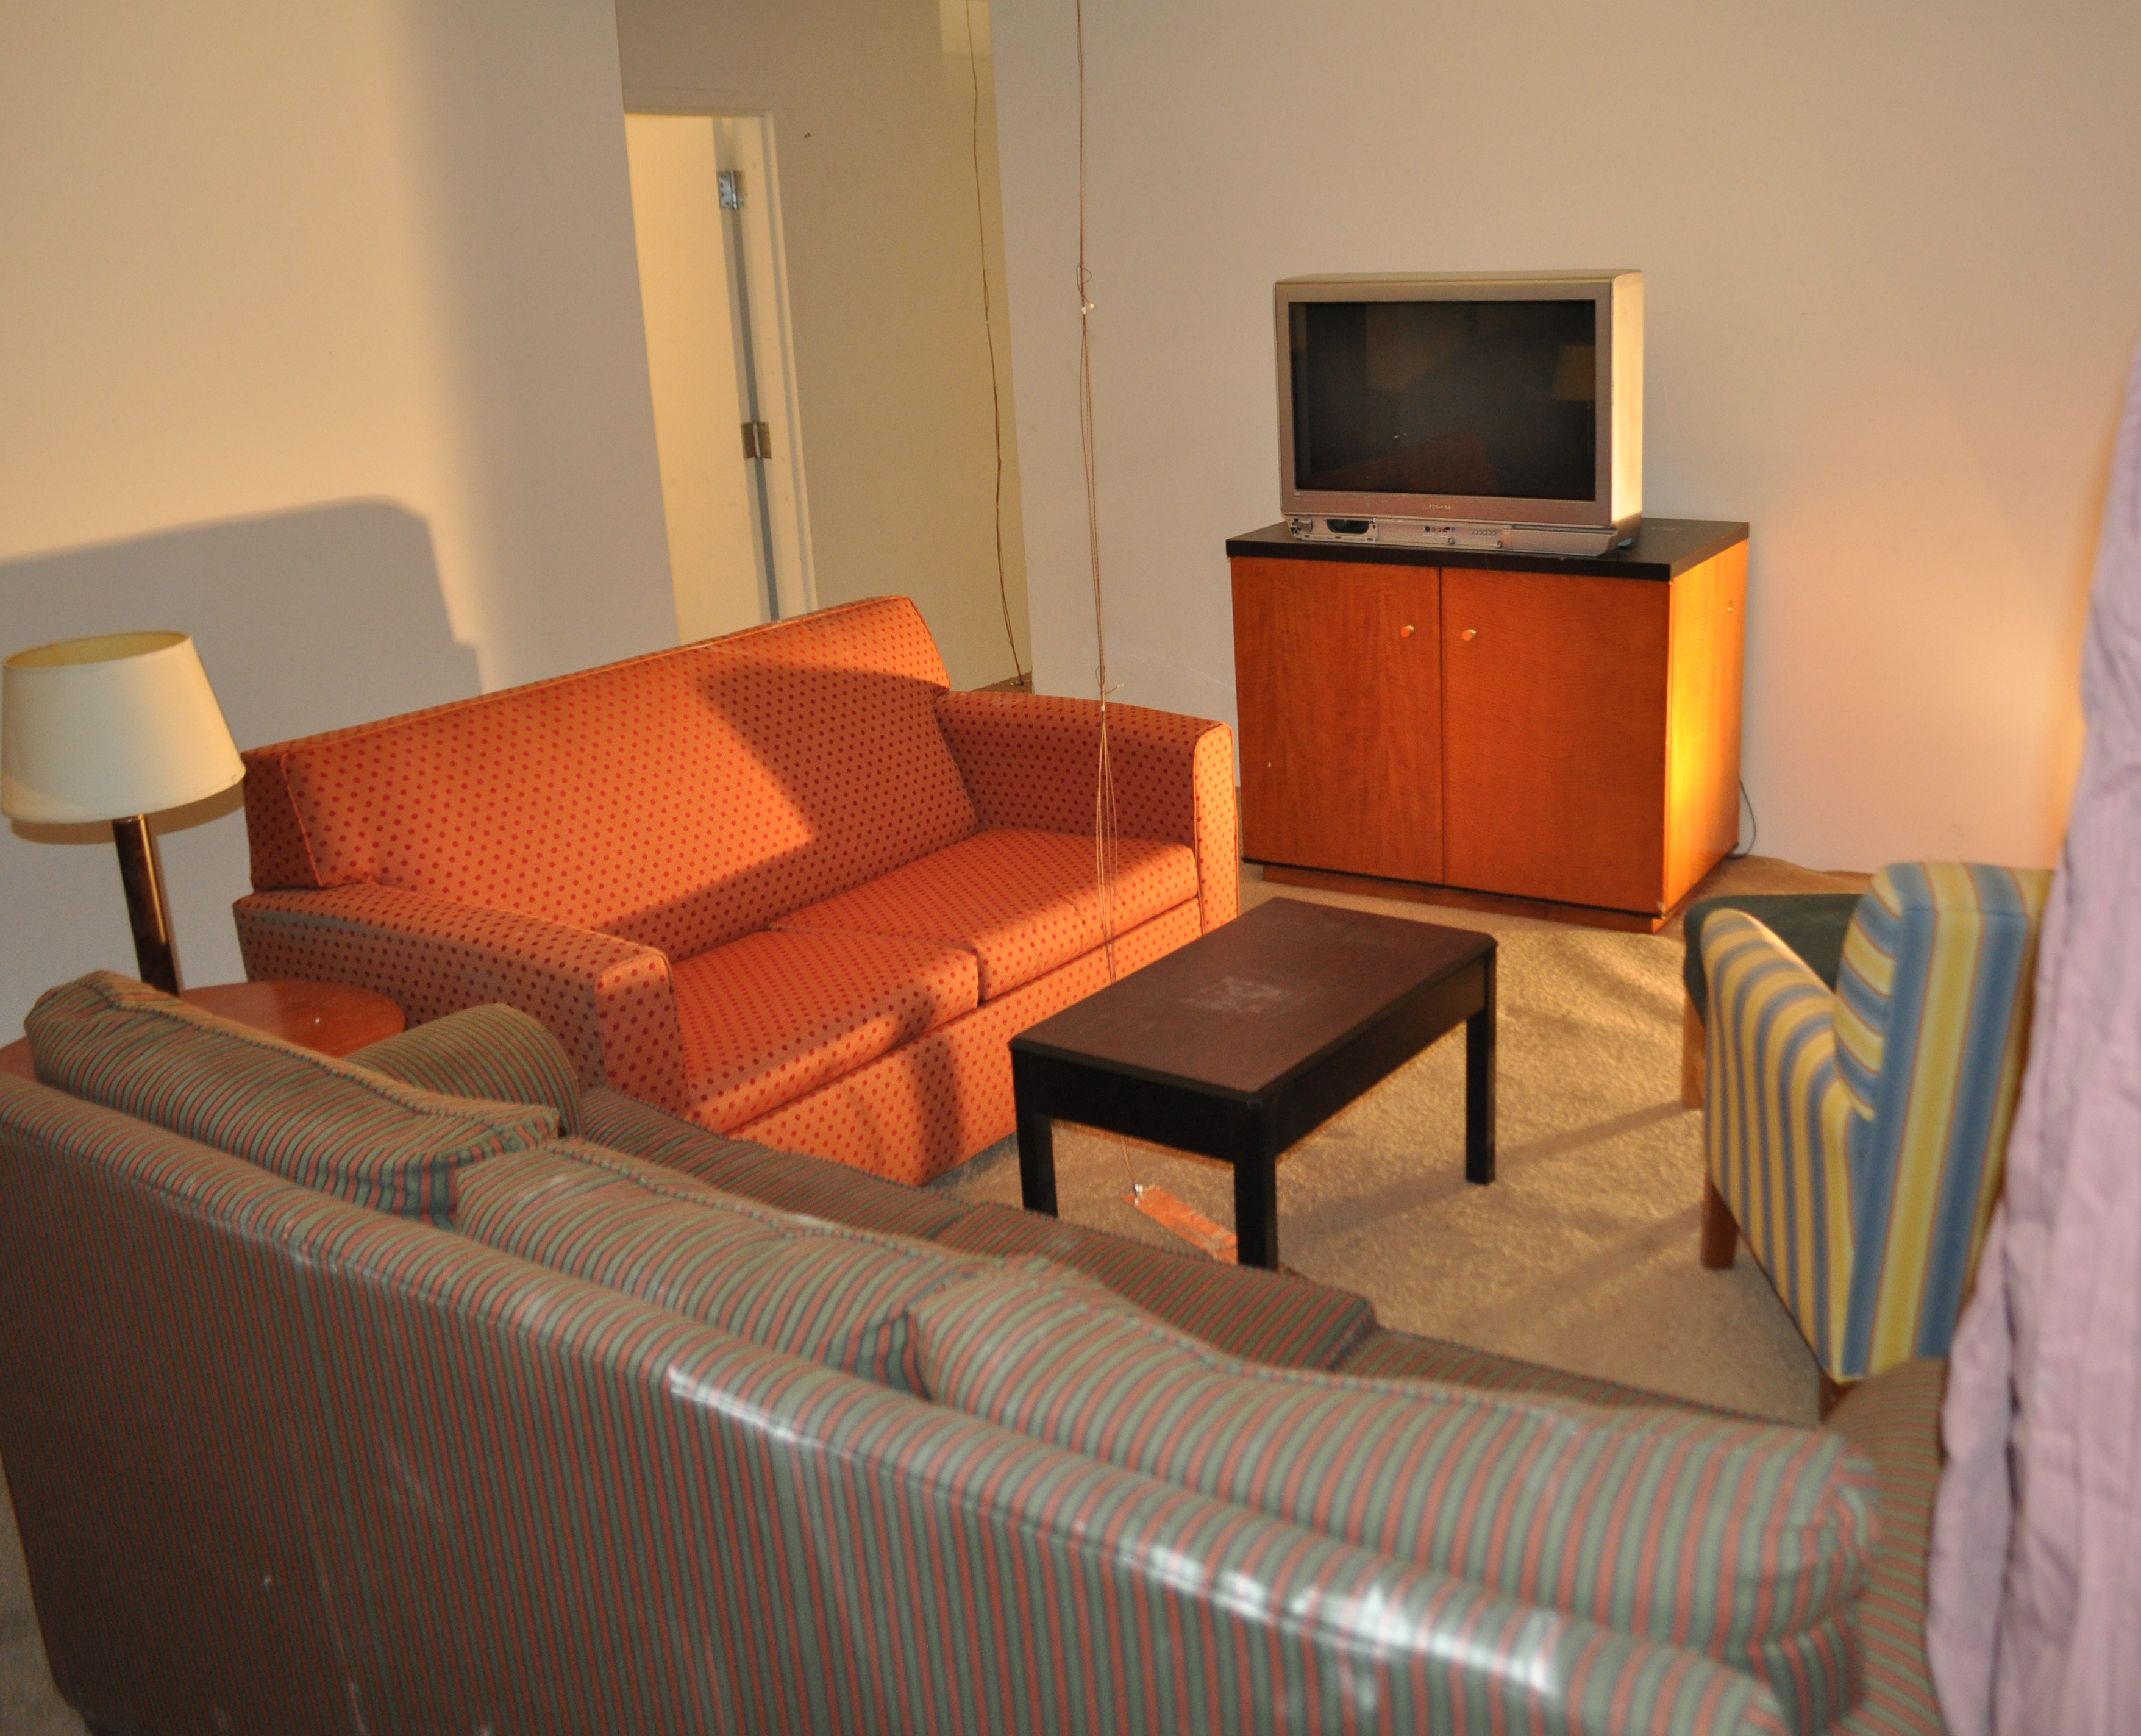
\includegraphics[width=3in]{0_Images/Furniture/SingleStoryLivingRoom.jpg}} &
		\subfloat[Two Story Family Room]{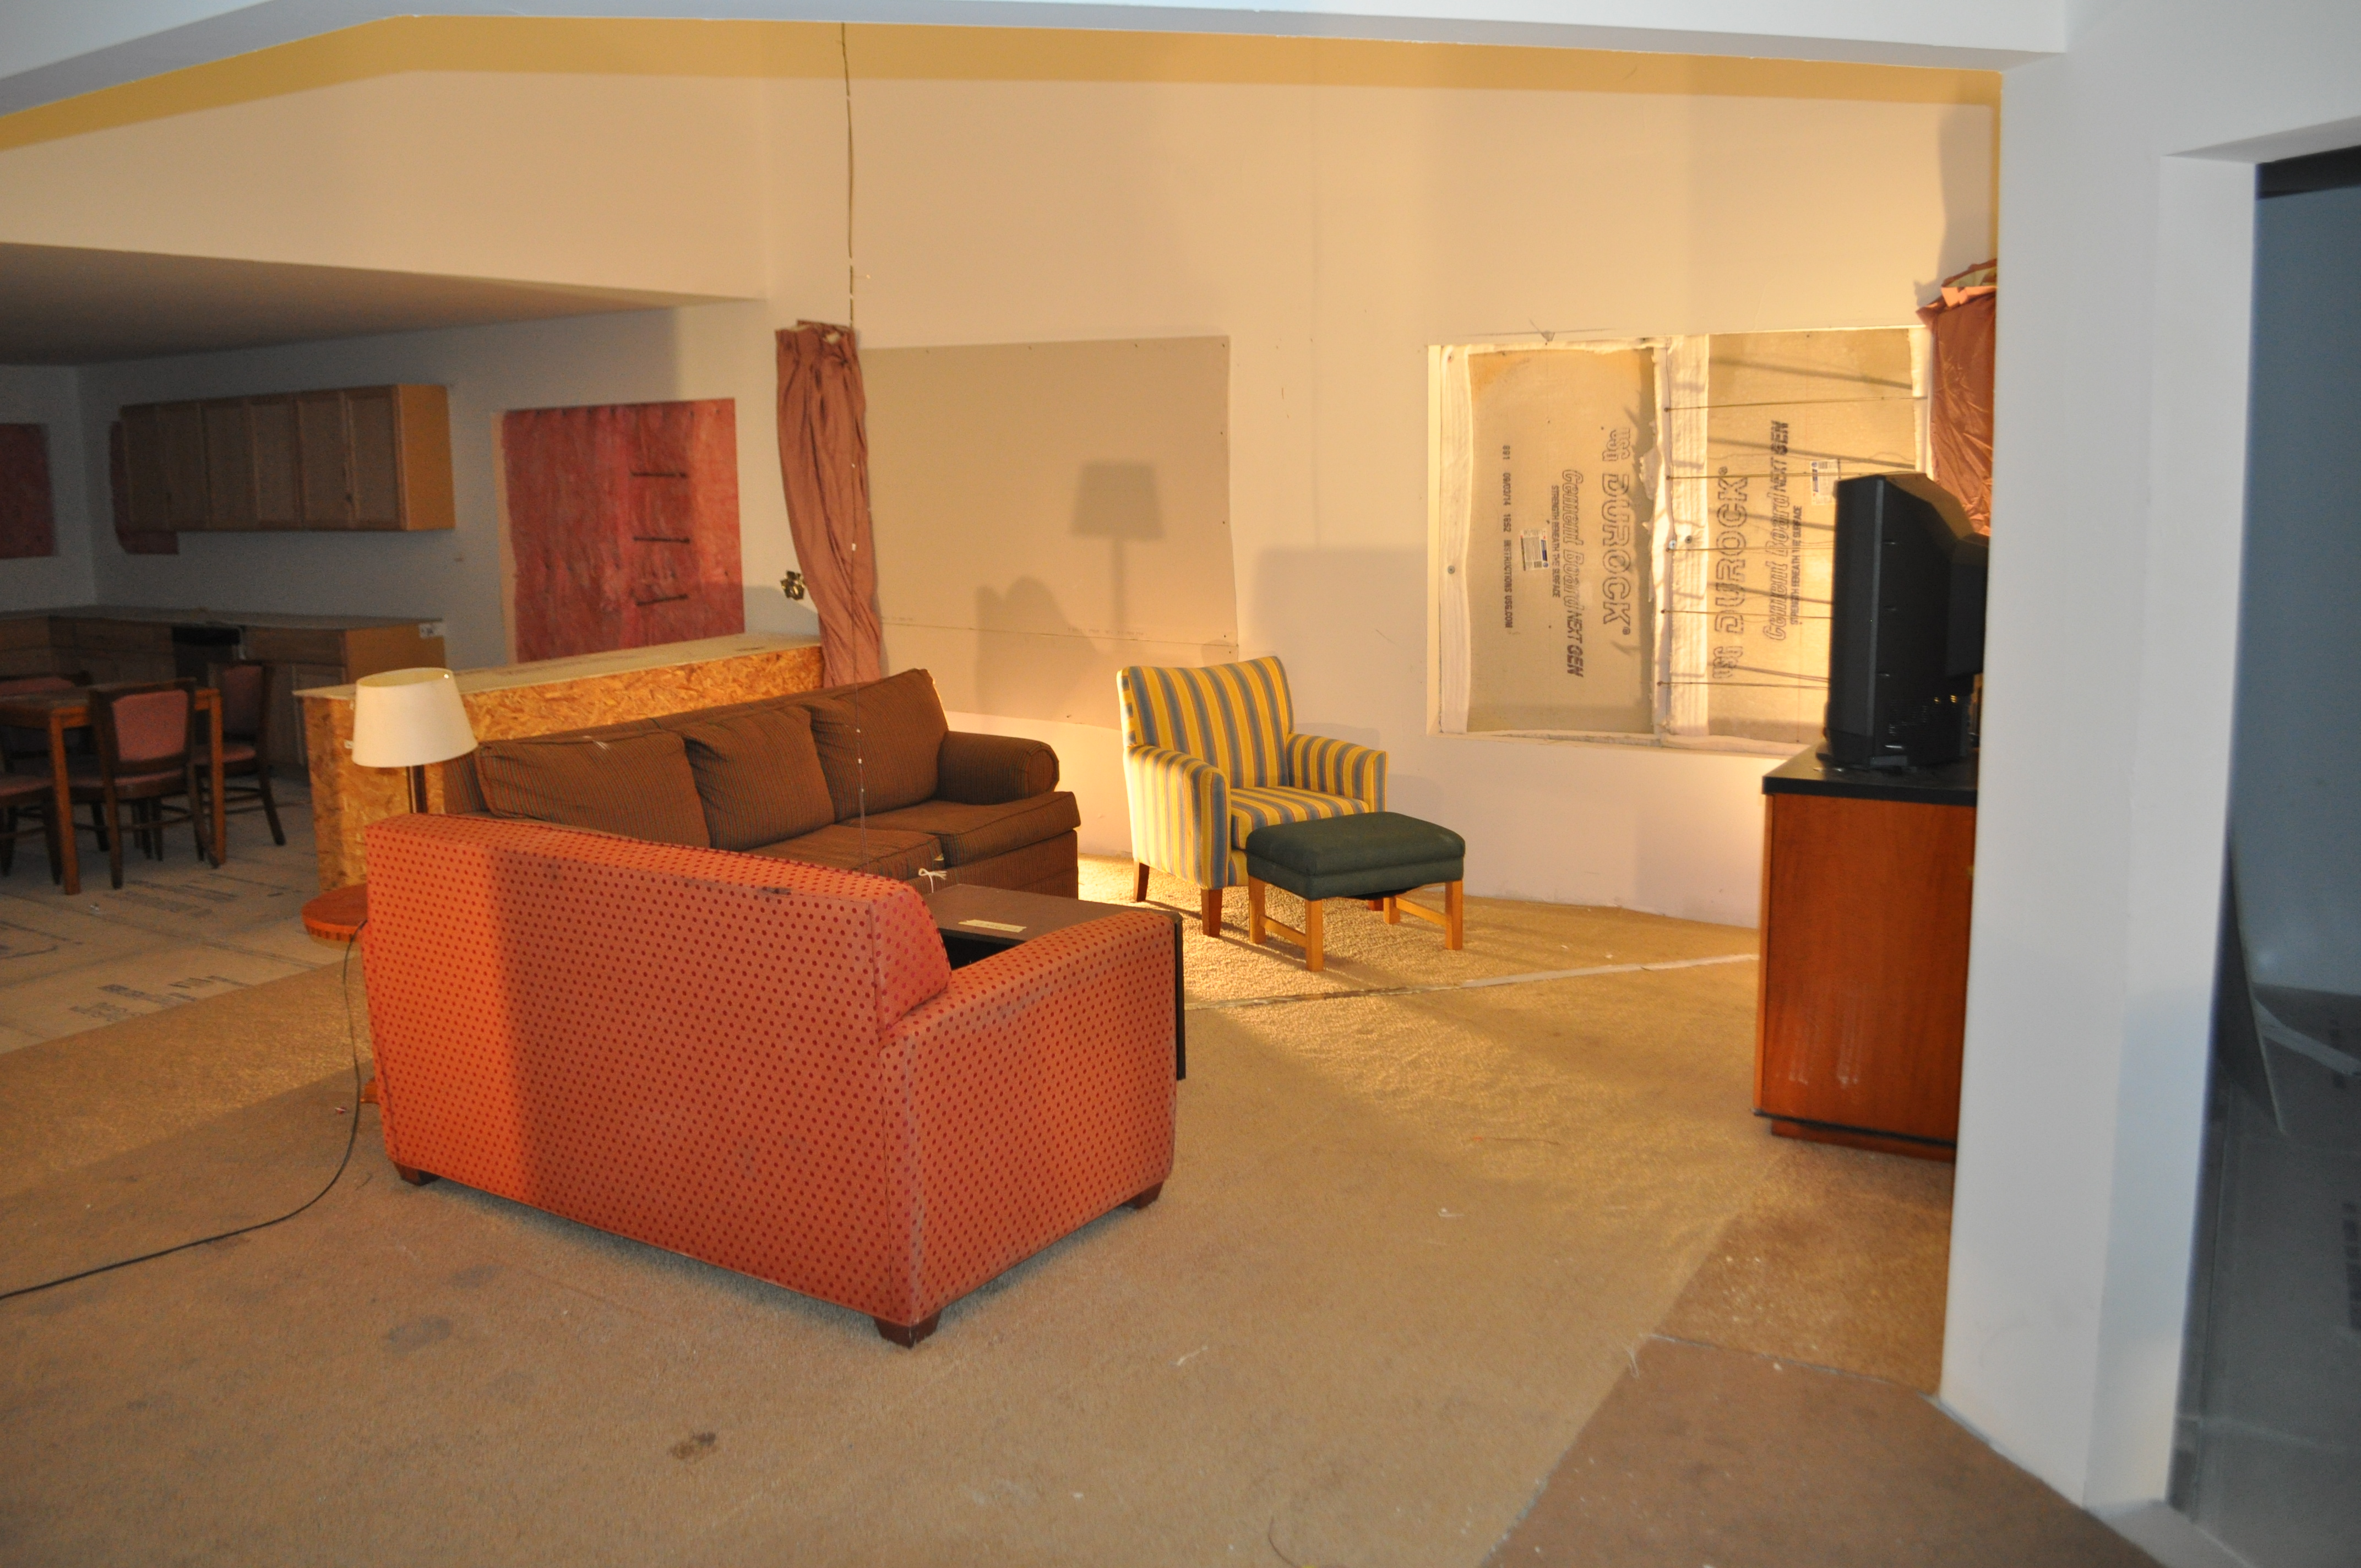
\includegraphics[width=3in]{0_Images/Furniture/TwoStoryFamilyRoom.jpg}} \\
	\end{tabular}
	\caption{Living \& Family Room Furniture}
	\label{fig:Living_Family}
\end{figure}

The master bedroom in both houses was furnished with a queen bed comprised of a mattress, box spring, wood frame, two pillows and comforter.  The rest of the room had a dark brown dresser and television. In th Single Story the master bedroom also contained a brown chair.  The floor was covered with polyurethane foam padding and polyester carpet. Figure \ref{fig:MasterBedrooms} shows the master bedroom furniture setup in both the single story and two story.

\begin{figure}[H]
	\centering
	\begin{tabular}[c]{c c}
		\subfloat[Single Story Master]{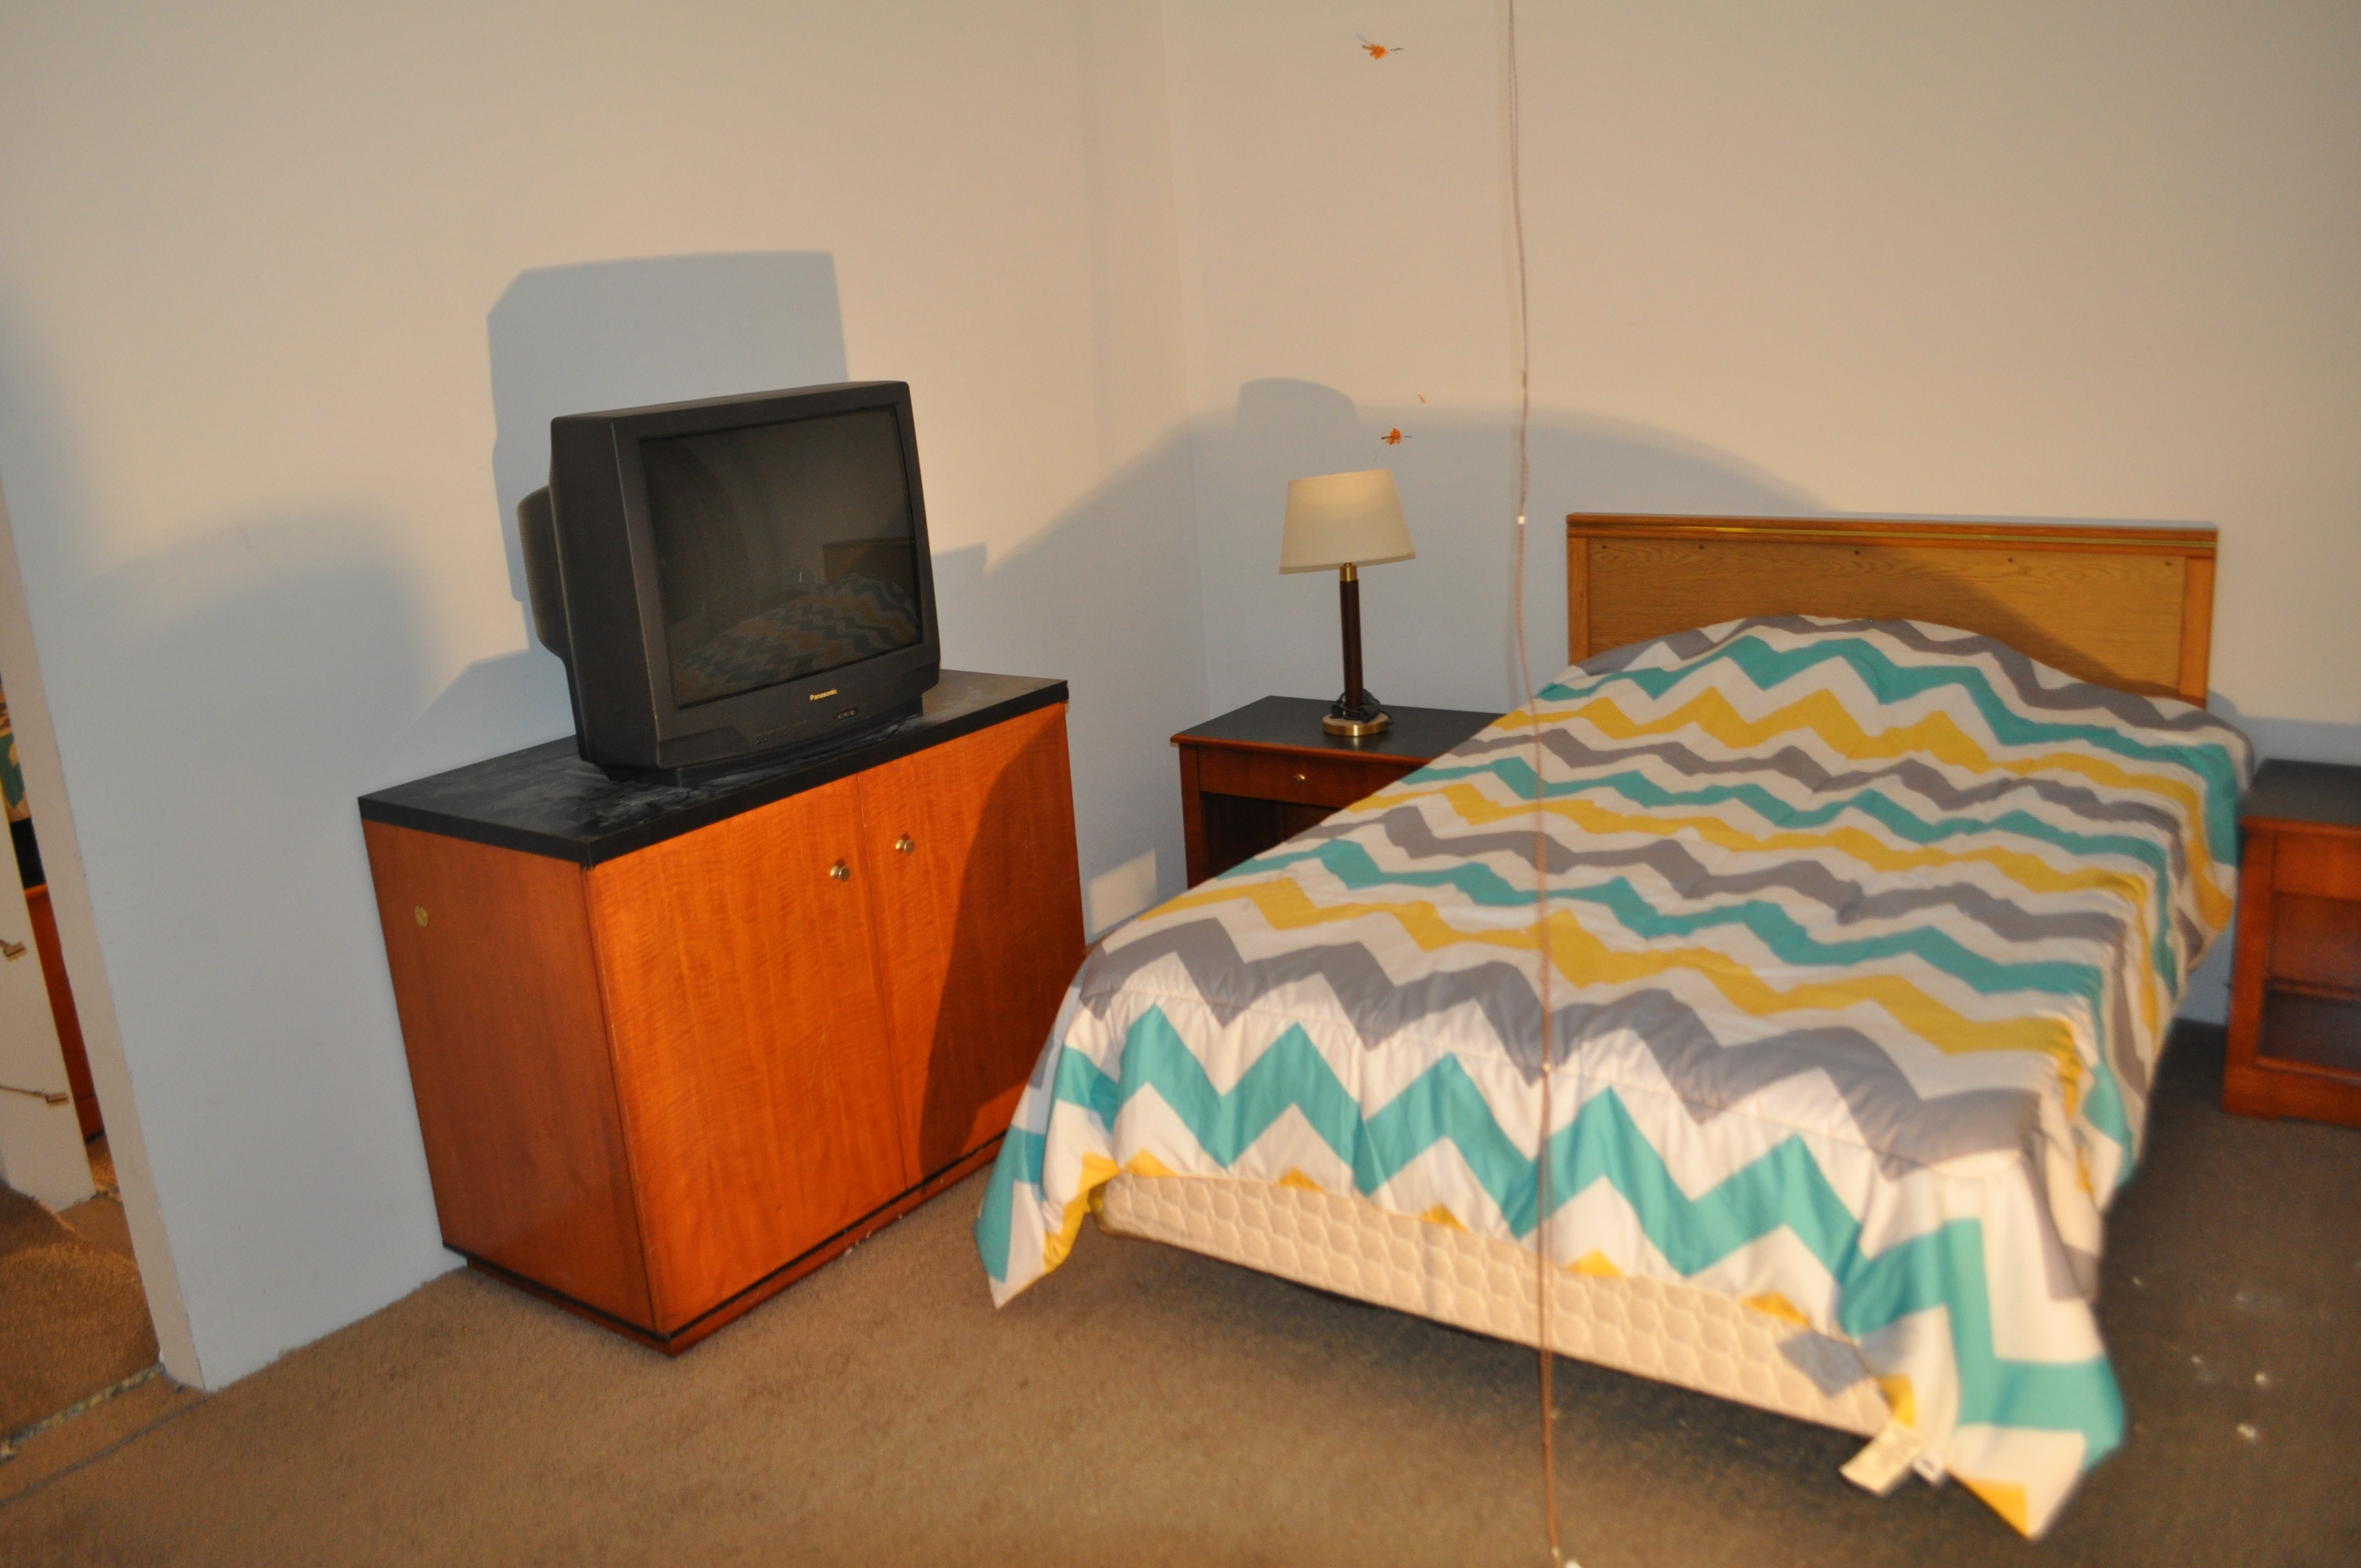
\includegraphics[width=3in]{0_Images/Furniture/1StoryMaster.jpg}} &
		\subfloat[Two Story Master]{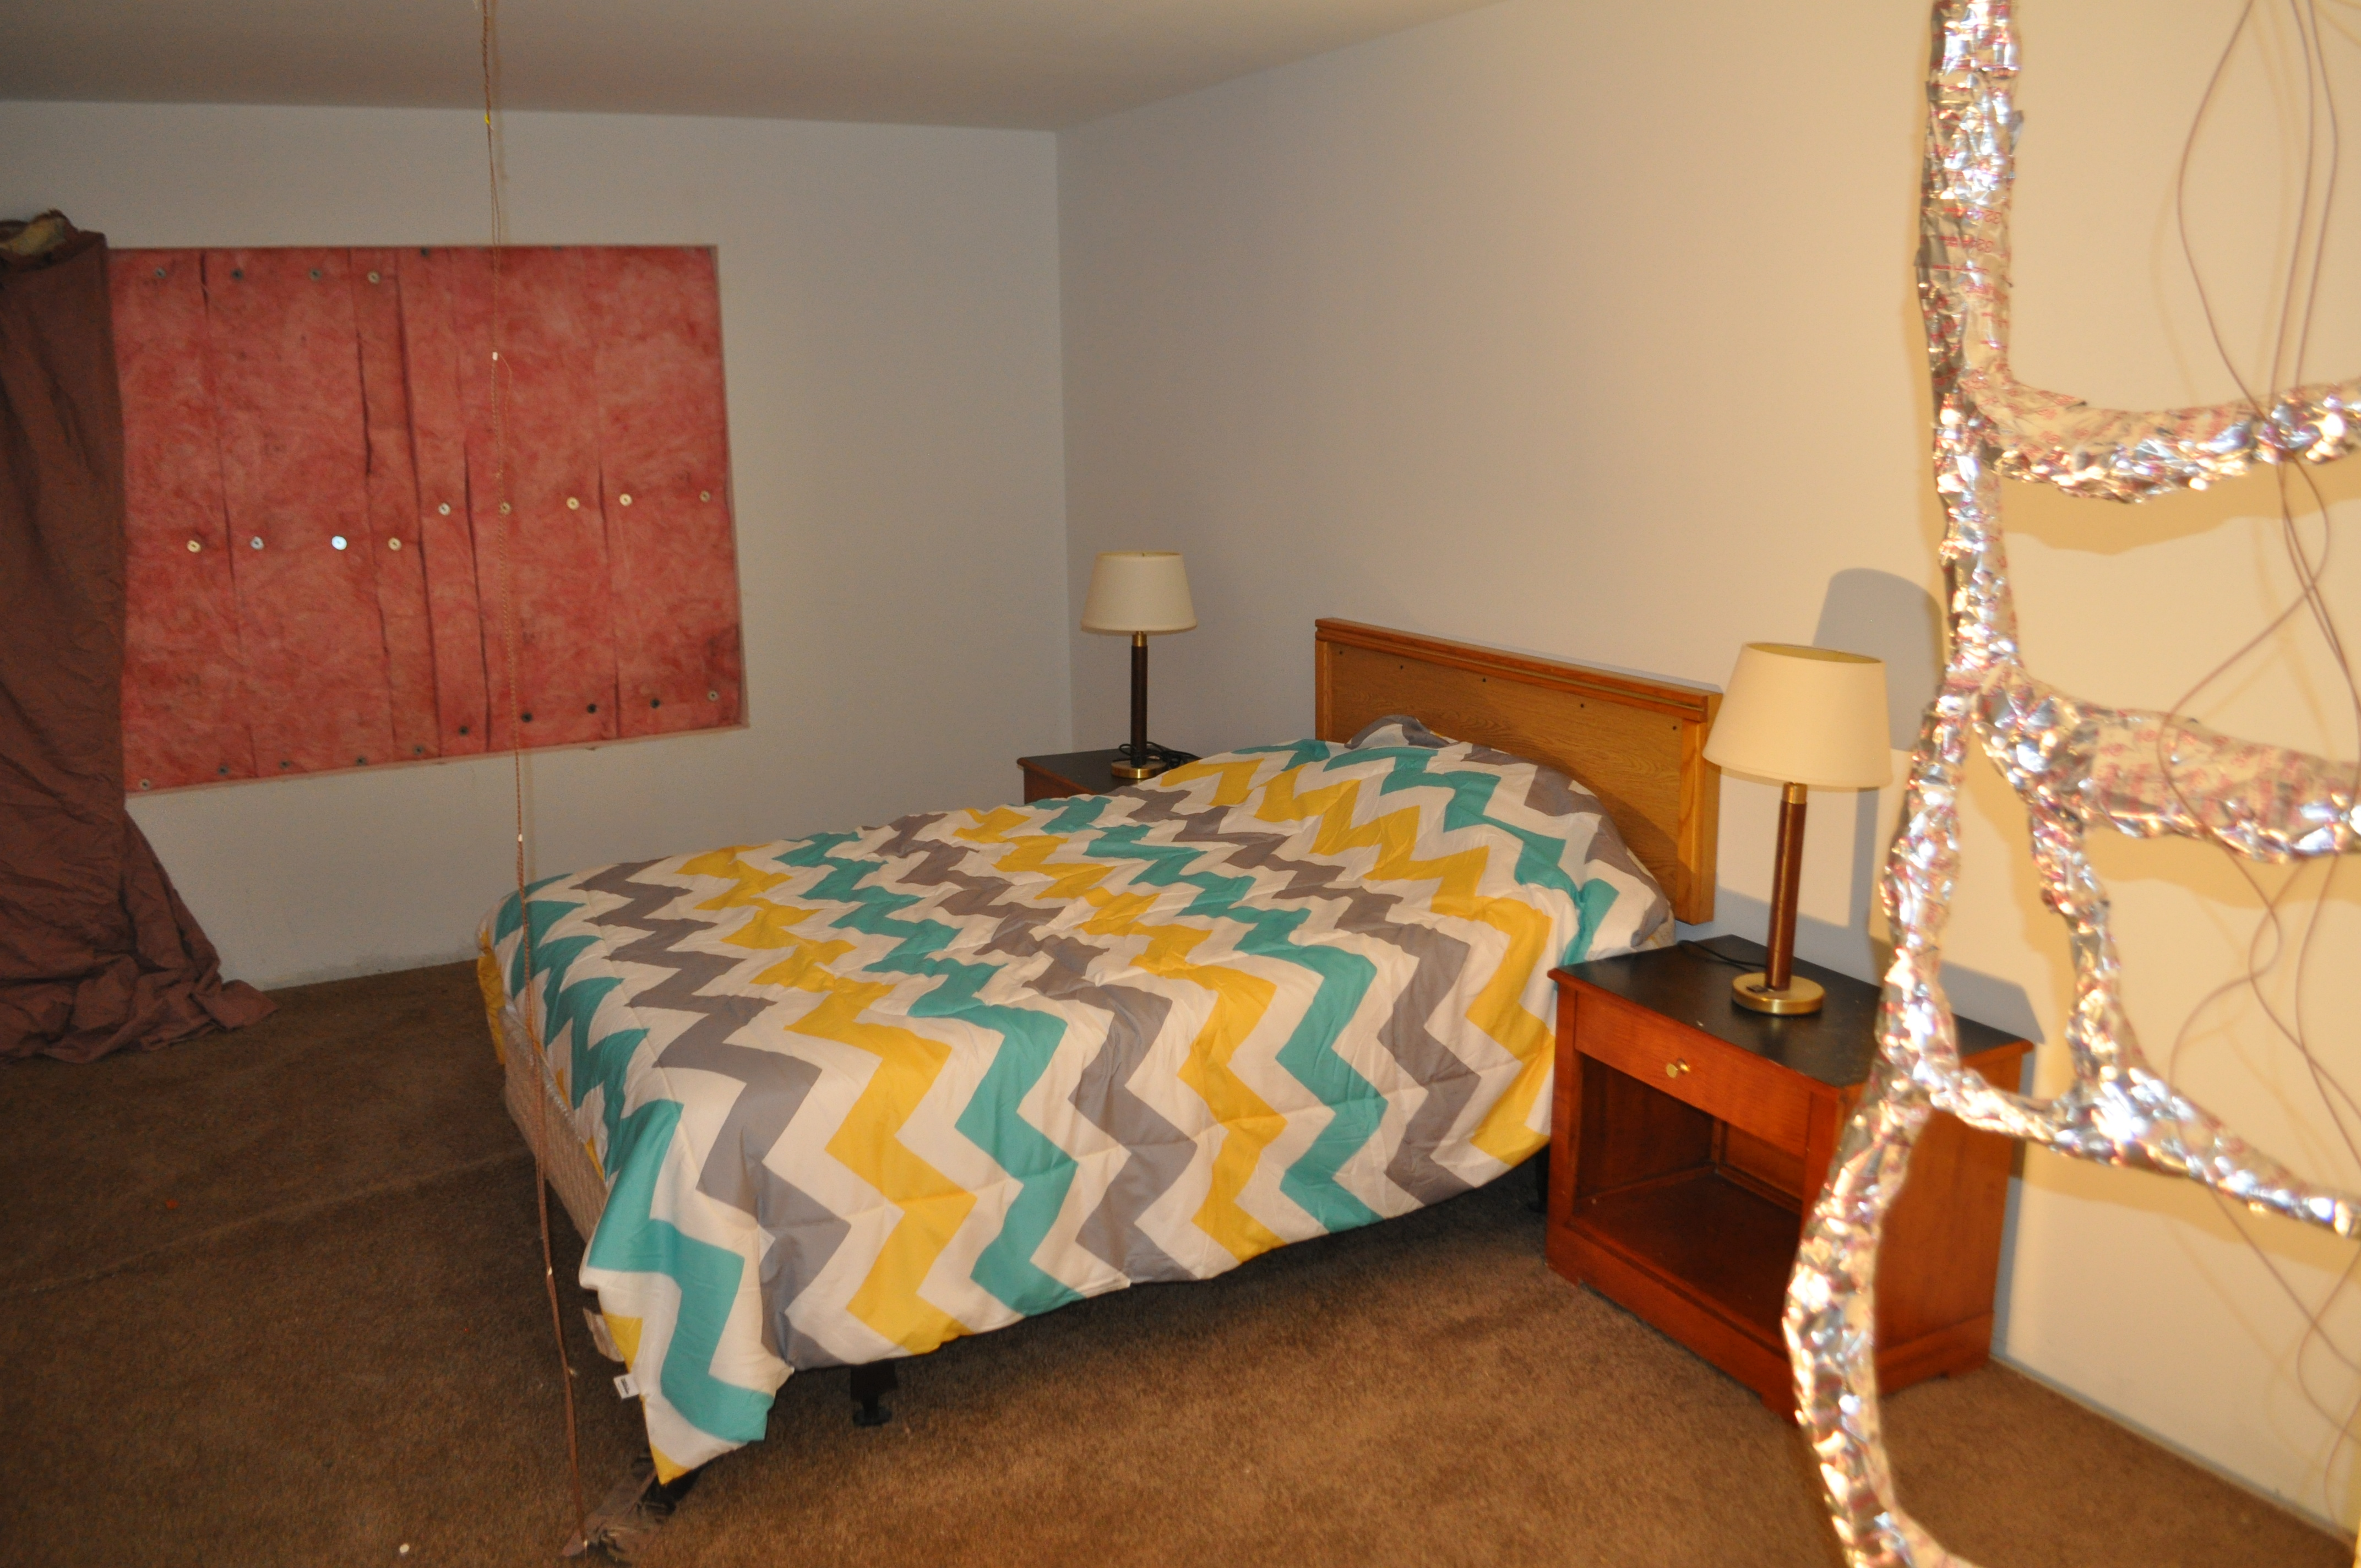
\includegraphics[width=3in]{0_Images/Furniture/2StoryMaster.jpg}} \\
	\end{tabular}
	\caption{Master Bedroom Furniture}
	\label{fig:MasterBedrooms}
\end{figure}

The remainder of the bedrooms in both houses were furnished with the same bed, television stand, television and flooring compliment as well as a light brown dresser, and headboard. For fires located in the bedrooms an additional mattress was added to the bed to extend burn duration. Figure \ref{fig:Bedrooms} shows the furniture setup for both the single story and two story bedrooms. 

\begin{figure}[H]
	\centering
	\begin{tabular}[c]{c c}
		\subfloat[Single Story Bedroom 2]{\includegraphics[width=3in]{0_Images/Furniture/1StoryBed2.jpg}} &
		\subfloat[Single Story Bedroom 3]{\includegraphics[width=1.5in]{0_Images/Furniture/1StoryBed3.jpg}} \\
		\subfloat[Two Story Bedroom 2]{\includegraphics[width=3in]{0_Images/Furniture/2StoryBed2.jpg}} &
		\subfloat[Two Story Bedroom 3]{\includegraphics[width=3in]{0_Images/Furniture/2StoryBed3.jpg}} \\
	\end{tabular}
	\centering	
	\subfloat[Two Story Bedroom 4]{\includegraphics[width=3in]{0_Images/Furniture/2StoryBed4.jpg}} \\
	\caption{Bedroom Furniture}
	\label{fig:Bedrooms}
\end{figure}

The dining room of both houses was furnished with two solid wood tables put together as a single table and six kitchen chairs. The tables were centered in the space with the chairs surrounding them. Figure \ref{fig:Dinning} shows the furniture setup for both the single story and two story dining rooms. 

\begin{figure}[H]
	\centering
	\begin{tabular}[c]{c c}
		\subfloat[Single Story Dining]{\includegraphics[width=3in]{0_Images/Furniture/1StoryDining.jpg}} &
		\subfloat[Two Story Dining]{\includegraphics[width=3in]{0_Images/Furniture/2StoryDining.jpg}} \\
	\end{tabular}
	\caption{Dining Room Furniture}
	\label{fig:Dinning}
\end{figure}

The kitchen in the single story was furnished with one table two chairs as the eat in table, as well as a dishwasher, stove, refrigerator and kitchen cabinets with cement board counters. The same appliances, cabinets and counter tops were found in the two story structure with a single table and four chairs. The floors of both rooms were cement board to simulate a tile floor.  Figure \ref{fig:Kitchen} shows the cabinet layout for both the single story and two story kitchens.

\begin{figure}[H]
	\centering
	\begin{tabular}[c]{c c}
		\subfloat[Single Story Kitchen]{\includegraphics[width=3in]{0_Images/Furniture/1StoryKitchen.jpg}} &
		\subfloat[Two Story Kitchen]{\includegraphics[width=3in]{0_Images/Furniture/2StoryKitchen.jpg}} \\
	\end{tabular}
	\caption{Kitchen Layout}
	\label{fig:Kitchen}
\end{figure}

\begin{figure}[H]
	\centering
	\includegraphics[width=\textwidth]{0_Images/Furniture/Single_Story_Furniture_Layout.pdf}
	\caption{Single Story Furniture Layout}
	\label{fig:SingleStoryFurniture}
\end{figure}

For exact locations and exact quantities of furniture see Figure \ref{fig:SingleStoryFurniture} and Figure \ref{fig:TwoStoryFurniture} for layout and dimensions of furniture. 

\begin{figure}[H]
	\centering
	\includegraphics[width=\textwidth]{0_Images/Furniture/Two_Story_Furniture_Layout.pdf}
	\caption{Two Story Furniture Layout}
	\label{fig:TwoStoryFurniture}
\end{figure}

\subsection{Measurement Locations}

\paragraph{Single Story} \mbox{}\\
The single story structure was instrumented with temperature, air flow, pressure and gas sensors to evaluate the temperature, gas flow, pressure and gas concentration. 

Temperature was measured via Type K thermocouple arrays. Each array contained 4 measurement points at 1ft, 3ft, 5ft and 7ft above the floor level. An array was located near the center of the living room, hallway, master bedroom, bedroom 2, bedroom 3, kitchen, and dining room.    

Air flow was measured via bi-directional probes. The front, bedroom 2, bedroom 3, and master bedroom doorways were instrumented with five bi-directional probes arrayed vertically along the center line at 8in, 24in, 30in, 46in and 62in above the floor. In addition the living room, master bedroom, bedroom 2 and bedroom 3 windows were instrumented with five bi-directional probes arrayed vertically along the center line at 6in, 18in, 30in, 42in and 54in above the window sill. 

Pressure was recorded through a differential pressure transducer in the living room, dining room, kitchen, master bedroom, bedroom 2 and bedroom 3 at 12in, 48in and 84in above the floor. 

Gas sample points were located in the hallway, dining room, bedroom 2 and bedroom 3. The probes were located in the corner, 1ft off of each wall and 1ft off the floor. Sample ports were connected back to the gas analyzers located on the exterior of the structure. 

The locations of each sensor is shown in Figure \ref{fig:SingleStoryInst}.

\begin{figure}[H]
	\centering
	\includegraphics[width = 3.5in]{0_Images/Instrumentation/Single_Story_Instrumentation.png}
	\includegraphics[width = 1.75in]{0_Images/Instrumentation/Single_Story_Instrumentation_Key2.png}
	\caption{Single Story Instrumentation}
	\label{fig:SingleStoryInst}
\end{figure}

\paragraph{Two Story} \mbox{}\\
The two story structure was instrumented with temperature, air flow, pressure and gas sensors to evaluate the temperature, gas flow, pressure and gas concentration. 

Temperature was measured via Type K thermocouple arrays. An array containing 4 measurement points at 1ft, 3ft, 5ft and 7ft above the floor level. An array was located near the center of the the living room, kitchen, dining room, den, hallway, master bedroom, bedroom 2, bedroom 3 and bedroom 4. An array containing 8 measurement points at 1ft, 3ft, 5ft, 7ft, 9ft, 11ft, 13ft and 15ft above the floor level in the family room, and foyer.

Air flow was measured via bi-directional probes. The front, bedroom 3, and master bedroom doorways were instrumented with five bi-directional probes arrayed vertically along the center line at 8in, 24in, 30in, 46in and 62in above the floor. In addition the both family room, and the bedroom 3 windows were instrumented with five bi-directional probes arrayed vertically along the center line at 6in, 18in, 30in, 42in and 54in above the window sill. 

Pressure was recorded through a differential pressure transducer in the den , master bedroom, bedroom 2 and bedroom 3 at 12in, 48in and 84in above the floor. 

Gas sample points were located in the hallway, dining room, bedroom 2 and bedroom 3. The probes were located in the corner, 1ft off of each wall and 1ft off the floor. Sample ports were connected back to the gas analyzers located on the exterior of the structure. 

The locations of each sensor is shown in Figure \ref{fig:TwoStoryInst}.

\begin{figure}[H]
	\centering
	\includegraphics[width = 1.75in]{0_Images/Instrumentation/Single_Story_Instrumentation_Key2.png} \\
	\begin{tabular}{*2c}
		\subfloat[First Floor]{\includegraphics[width = 3.0in]{0_Images/Instrumentation/Two_Story.png}} &
		\subfloat[Second Floor]{\includegraphics[width = 3.0in]{0_Images/Instrumentation/Two_Story2.png}} \\
	\end{tabular}
	\caption{Two Story Instrumentation}
	\label{fig:TwoStoryInst}
\end{figure}

\clearpage

\section{Heat Release Fuel Load Characterization} \mbox{}

To characterize the upholstered furniture energy release rates, heat release rate burns were conducted under a cone calorimeter hood. Each piece of furniture was permitted to burn down until a smoldering fire was observed. Table \ref{table:FurnitureHRR_Data} shows the furniture tested and peak heat release rate, total energy released and burnout time for each piece of furniture tested. Table \ref{table:FurnitureHRR_Data} shows the peak heat release rate, total energy released, and burn duration for each of the upholstered furniture types used in the fuel load. 

\begin{table}[H]
	\caption{Furniture Heat Release Data}
	\begin{tabular}{|c|c|c|c|}
		\hline
		Furniture & Peak Heat Release Rate (kW) & Total Energy Released (MJ) & Burn duration \\ \hline \hline
		Chair (Yellow) 1 & 845 & 145 & 14:45 \\ \hline
		Chair (Yellow) 2 & 1094 & 123 & 15:00 \\ \hline
		Chair (Yellow) 3 & 1236 & 128 & 15:00 \\ \hline
		Chair (Brown) 1 & 1841 & 458 & 19:45 \\ \hline
		Chair (Brown) 2 & 1473 & 451 & 19:45 \\ \hline
		Chair (Brown) 3 & 1410 & 391 & 19:45 \\ \hline
		Sleeper Sofa (Orange) 1  & 2441 & 632 & 22:46 \\ \hline
		Sleeper Sofa (Orange) 2  & 1897 & 663 & 22:44 \\ \hline
		Sleeper Sofa (Orange) 3  & 2083 & 613 & 23:10 \\ \hline
		Sleeper Sofa (Green) 1  & 3543 & 968 & 24:44 \\ \hline
		Sleeper Sofa (Green) 2  & 2894 & 1071 & 24:44 \\ \hline
		Sleeper Sofa (Green) 3  & 2640 & 1071 & 24:45 \\ \hline
		Bed 1 & 1306 & 873 & 50:00 \\ \hline
		Bed 2 & 1399 & 709 & 53:23 \\ \hline
	\end{tabular}
	\label{table:FurnitureHRR_Data}
\end{table}

\clearpage

The results of the Chair (Yellow) heat release rate characterization burns is shown in Figure \ref{fig:YellowChairHRR}. The growth of the Chair (Yellow) was very similar with all three chairs tested with peak heat release rates occurring within 5 minutes to 5 minutes and 30 seconds of ignition. The Yellow Chair 3 grew slightly slower however provided the highest total energy released. Results for peak heat release rate were within 391kW between minimum and maximum, the total energy released was within 22MJ between the minimum and maximum. 

\begin{figure}[H]
	\centering
	\includegraphics[width=\textwidth]{0_Images/Furniture/ChairYellow_HRR.pdf}
	\caption{Chair (Yellow) Heat Release Rate Characterization Results}
	\label{fig:YellowChairHRR}
\end{figure}

The results of the Chair (Brown) heat release rate characterization burns is shown in Figure \ref{fig:BrownChairHRR}. The growth of the Chair (Brown) was very similar with all three chairs tested with peak heat release rates occurring within 4 and 45 Seconds to 5 minutes of ignition. The Brown Chair 1 grew slightly faster however provided the same total energy released as the Brown Chair 2. The Brown Chair 3 grew the slowest and provided the smallest total energy release. Results for peak heat release rate were within 431kW between minimum and maximum, the total energy released was within 67MJ between the minimum and maximum. 

\begin{figure}[H]
	\centering
	\includegraphics[height=0.45\textheight]{0_Images/Furniture/BrownChair_HRR.pdf}
	\caption{Chair (Brown) Heat Release Rate Characterization Results}
	\label{fig:BrownChairHRR}
\end{figure}

The results of the Sleeper Sofa (Orange) heat release rate characterization burns is shown in Figure \ref{fig:SofaOrangeHRR}. The growth of the Sleeper Sofa (Orange) was very similar with all three chairs tested with peak heat release rates occurring within 5 and 50 Seconds to 5 minutes and 10 seconds of ignition. Results for peak heat release rate were within 544kW between minimum and maximum, the total energy released was within 50MJ of between the minimum and maximum. 

\begin{figure}[H]
	\centering
	\includegraphics[height=0.45\textheight]{0_Images/Furniture/Sofa_Orange_HRR.pdf}
	\caption{Sleeper Sofa (Orange) Heat Release Rate Characterization Results}
	\label{fig:SofaOrangeHRR}
\end{figure}

The results of the Sleeper Sofa (Green) heat release rate characterization burns is shown in Figure \ref{fig:SofaGreenHRR}. The growth of the Sleeper Sofa was very similar with all three chairs tested with peak heat release rates occurring within 6 to 7 minutes of ignition. Results for peak heat release rate were within 903kW between minimum and maximum, the total energy released was within 103MJ of between the minimum and maximum. 

\begin{figure}[H]
	\centering
	\includegraphics[height=0.45\textheight]{0_Images/Furniture/Sofa_Green_HRR.pdf}
	\caption{Sleeper Sofa (Green) Heat Release Rate Characterization Results}
	\label{fig:SofaGreenHRR}
\end{figure}

The results of the bed heat release rate characterization burns is shown in Figure \ref{fig:BedHRR}. The growth of the Beds was significantly different as the fire had to burn across the top of the comforter and down before involving the matress and reaching its peak heat release rate at approximately 38 minutes for bed 1 and 45 minutes for bed 2. Although the growth rate differed the results of the peak heat release rate were within 93kW between minimum and maximum, the total energy released was within 164MJ of between the minimum and maximum. The difference in the total energy release can be explained due to the different growth rates and time frame associated with each.

\begin{figure}[H]
	\centering
	\includegraphics[height=0.45\textheight]{0_Images/Furniture/Bed_HRR.pdf}
	\caption{Bed Heat Release Rate Characterization Results}
	\label{fig:BedHRR}
\end{figure}

\subsection{Ventilation Limited Room Burns}
A fire burns in direct proportion to the available oxygen. Past studies conducted under the Department of Homeland Securities Assistance to firefighters grants have established a basis of this for both single compartment fires along with fires within a residential structure \cite{DHS2008} \cite{DHS2010}. In order to provide further understanding of this concept two room scale experiments were conducted under a cone calorimeter hood to evaluate the energy release rate as it compares to the fuel load in a furnished as compared to an over furnished compartment with the same ventilation opening.

Each compartment measured 12ft long by 12ft wide and 8ft tall, with a front opening of 7ft - 10$\frac{3}{4}$in wide by 8ft high. The walls were wood stud frame 16in on center with $\frac{1}{2}$in type X gypsum wall board. The ceiling was supported by 2in x 6in framing 16in on center with a type X gypsum wall board. The floor was concrete covered with a $\frac{1}{2}$in cement board. The compartments were constructed side by side in the oxygen consumption calorimeter lab at UL's Northbrook test facility. 

\paragraph{Furnished Compartment} \mbox{}

The furnished compartment contained a sofa and arm chair, coffee table, TV Stand, tube television, two plastic bins, two end tables, lamp and stuffed toys, picture frames, candles, drapes and a polyester carpet. See Figure \ref{fig:furnished_images} for arrangement of furnishings and Figure \ref{fig:furnished_layout} for dimensions and furniture layout.

\begin{figure}[H]
	\centering
	\begin{tabular} {c c c}
	\subfloat[]{\includegraphics[width=5cm]{0_Images/Vent_Limited_Room/Furnished_Overall.jpg}} &
	\subfloat[]{\includegraphics[width=5cm]{0_Images/Vent_Limited_Room/Furnished_Left_Side.jpg}} &
	\subfloat[]{\includegraphics[width=5cm]{0_Images/Vent_Limited_Room/Furnished_Center.jpg}} \\
	\end{tabular}
	\begin{tabular} { c c }
	\subfloat[]{\includegraphics[width=5cm]{0_Images/Vent_Limited_Room/Furnished_Center_Right.jpg}} &
	\subfloat[]{\includegraphics[width=5cm]{0_Images/Vent_Limited_Room/Furnished_Right_Side.jpg}} \\
	\end{tabular}
	\caption{Furnished Room Images}
	\label{fig:furnished_images}
\end{figure}

\begin{figure}[H]
	\centering
	\includegraphics[width=3in]{0_Images/Vent_Limited_Room/Furnished_Room.jpg}
	\caption{Furnished Room Layout}
	\label{fig:furnished_layout}
\end{figure}

Ignition for the furnished compartment occurred in the back left corner of the couch up against the arm using a standard flame butane flame. The room was permitted to burn completely out over a duration of 12 minutes and 45 seconds. Figure \ref{fig:furnished_screenshots}  shows the experiment results every 30 seconds up until flash over and then in one minute increments following flash over. 


\begin{figure}[H]
	\centering
	\begin{tabular} {c c c}
		\subfloat[00:00]{\includegraphics[width=3.9cm]{0_Images/Vent_Limited_Room/furnished_screenshot(1).png}} &
		\subfloat[00:30]{\includegraphics[width=3.9cm]{0_Images/Vent_Limited_Room/furnished_screenshot(2).png}} &
		\subfloat[01:00]{\includegraphics[width=3.9cm]{0_Images/Vent_Limited_Room/furnished_screenshot(3).png}} \\
		\subfloat[01:30]{\includegraphics[width=3.9cm]{0_Images/Vent_Limited_Room/furnished_screenshot(4).png}} &
		\subfloat[02:00]{\includegraphics[width=3.9cm]{0_Images/Vent_Limited_Room/furnished_screenshot(5).png}} &
		\subfloat[02:30]{\includegraphics[width=3.9cm]{0_Images/Vent_Limited_Room/furnished_screenshot(6).png}} \\
		\subfloat[02:45]{\includegraphics[width=3.9cm]{0_Images/Vent_Limited_Room/furnished_screenshot(7).png}} &
		\subfloat[03:00]{\includegraphics[width=3.9cm]{0_Images/Vent_Limited_Room/furnished_screenshot(8).png}} &
		\subfloat[04:00]{\includegraphics[width=3.9cm]{0_Images/Vent_Limited_Room/furnished_screenshot(10).png}} \\
		\subfloat[05:00]{\includegraphics[width=3.9cm]{0_Images/Vent_Limited_Room/furnished_screenshot(11).png}} &
		\subfloat[06:00]{\includegraphics[width=3.9cm]{0_Images/Vent_Limited_Room/furnished_screenshot(12).png}} &
		\subfloat[07:00]{\includegraphics[width=3.9cm]{0_Images/Vent_Limited_Room/furnished_screenshot(13).png}} \\
		\subfloat[08:00]{\includegraphics[width=3.9cm]{0_Images/Vent_Limited_Room/furnished_screenshot(14).png}} &
		\subfloat[09:00]{\includegraphics[width=3.9cm]{0_Images/Vent_Limited_Room/furnished_screenshot(15).png}} &
		\subfloat[10:00]{\includegraphics[width=3.9cm]{0_Images/Vent_Limited_Room/furnished_screenshot(16).png}} \\
	\end{tabular}
	
	\begin{tabular}{c c}
		\subfloat[11:00]{\includegraphics[width=3.9cm]{0_Images/Vent_Limited_Room/furnished_screenshot(17).png}} &
		\subfloat[12:00]{\includegraphics[width=3.9cm]{0_Images/Vent_Limited_Room/furnished_screenshot(18).png}} \\	
	\end{tabular}
	
	\caption{Furnished Room Experiment Images}
	\label{fig:furnished_screenshots}
\end{figure}

\paragraph{Over Furnished Compartment} \mbox{}

The over furnished compartment contained six stuffed brown chairs, two orange sleeper sofas and two one green sleeper sofa from the furniture aquired for the full scale fire experiments. The furniture was arranged as shown in Figure \ref{fig:horder_images} with dimensions shown in Figure \ref{fig:horder_layout}.

\begin{figure}[H]
	\centering
	\begin{tabular} {c c c}
		\subfloat[]{\includegraphics[width=5cm]{0_Images/Vent_Limited_Room/Horder1.jpg}} &
		\subfloat[]{\includegraphics[width=5cm]{0_Images/Vent_Limited_Room/Horder2.jpg}} &
		\subfloat[]{\includegraphics[width=5cm]{0_Images/Vent_Limited_Room/Horder3.jpg}} \\
	\end{tabular}
	\caption{Over Furnished Compartment}
	\label{fig:horder_images}
\end{figure}

\begin{figure}[H]
	\centering
	\includegraphics[width=5in]{0_Images/Vent_Limited_Room/HorderRoom.jpg}
	\caption{Over Furnished Compartment Layout}
	\label{fig:horder_layout}
\end{figure}

The over furnished room was ignited in the left arm of the sofa against the rear wall with a butane flame and permitted to burn until a portion of the ceiling failed due to the fire in the compartment at 10 minutes and 10 seconds followed by an entire sheet of gypsum failing off the ceiling at 11 minutes and 30 seconds at which time the fire was extinguished. Figure \ref{fig:horder_screenshots} shows the the experiment every 1 minute along with 5 seconds after the first instance of ceiling failure at 10 minutes 15 seconds and again at 11 minutes and 37 seconds following the second failure.

\begin{figure}[H]
	\centering
	\begin{tabular} {c c c}
		\subfloat[00:00]{\includegraphics[width=3.9cm]{0_Images/Vent_Limited_Room/horder(1).png}} &
		\subfloat[01:00]{\includegraphics[width=3.9cm]{0_Images/Vent_Limited_Room/horder(2).png}} &
		\subfloat[02:00]{\includegraphics[width=3.9cm]{0_Images/Vent_Limited_Room/horder(3).png}} \\
		\subfloat[03:00]{\includegraphics[width=3.9cm]{0_Images/Vent_Limited_Room/horder(4).png}} &
		\subfloat[04:00]{\includegraphics[width=3.9cm]{0_Images/Vent_Limited_Room/horder(5).png}} &
		\subfloat[05:30]{\includegraphics[width=3.9cm]{0_Images/Vent_Limited_Room/horder(6).png}} \\
		\subfloat[06:00]{\includegraphics[width=3.9cm]{0_Images/Vent_Limited_Room/horder(7).png}} &
		\subfloat[07:00]{\includegraphics[width=3.9cm]{0_Images/Vent_Limited_Room/horder(8).png}} &
		\subfloat[08:00]{\includegraphics[width=3.9cm]{0_Images/Vent_Limited_Room/horder(9).png}} \\
		\subfloat[09:00]{\includegraphics[width=3.9cm]{0_Images/Vent_Limited_Room/horder(10).png}} &
		\subfloat[10:00]{\includegraphics[width=3.9cm]{0_Images/Vent_Limited_Room/horder(11).png}} &
		\subfloat[10:15]{\includegraphics[width=3.9cm]{0_Images/Vent_Limited_Room/horder(11a).png}} \\
	\end{tabular}
	
	\begin{tabular}{c c}
		\subfloat[11:00]{\includegraphics[width=3.9cm]{0_Images/Vent_Limited_Room/horder(12).png}} &
		\subfloat[11:37]{\includegraphics[width=3.9cm]{0_Images/Vent_Limited_Room/horder(13).png}} \\	
	\end{tabular}
	
	\caption{Overstuffed Room Experiment Images}
	\label{fig:horder_screenshots}
\end{figure}

\paragraph{Compartment Burn Results} \mbox{}

In each of the compartment burn the total heat release rate versus time was recorded via the oxygen consumption calorimeter. Although the compartment geometry was identical the fuel load was significantly different leading to two very different growth rates. As seen in Table \ref{table:comp_burn_results}, the furnished room reached its fully developed heat release rate at 2 minutes and 56 seconds where the over furnished room took longer to grow reaching its fully developed stage at 5 minutes and 46 seconds. The fully develop stage for both rooms was approximately 6500kW until the failure of the ceiling in the over furnished compartment failed increasing the available oxygen and thus the the heat release rate as seen in Figure \ref{fig:comp_burn_chart}. 

The difference in the two burns was the fuel configuration, which resulted in different growh rates (Figure \ref{fig:comp_burn_chart}) The furnished compartment reached a fully developed stage within 3 minutes of ignition and maintained that heat release rate for 3 minutes before it began to decay at 6 minutes. The over furnished compartment reached a similar peak heat release rate at just under 6 minutes and maintained that through the failure of the ceiling at 10 minutes at which time it increased. The over furnished compartment had more fuel to consume thus it remained fully developed much longer than the furnished compartment. 

With the same peak heat release rate the difference in the burns becomes the total energy release. The furnished compartment had a total energy release of approximately 2500MJ, where the total energy release for the over furnished compartment was approximately 3500MJ and it had yet to enter a fuel limited decay stage. The furnished compartment had entered its fuel limited decay stage (Figure \ref{fig:furnished_screenshots}) however in the over furnished compartment (Figure \ref{fig:horder_screenshots}) where there is still a substantial amount of fuel remaining at the time of ceiling failure. 

This demonstrates how the heat release rate or energy release rate in a compartment fire is limited by the available oxygen for combustion. The opening of the compartment served as the only means of supplying the fire with oxygen and limited its energy release. Additional fuel did not necessarily mean additional energy release per unit time, however it did mean additional energy release over the duration of the fire. 

\begin{table}[H]
	\caption{Compartment Burn Results}
	\begin{tabular}{|c|c|c|}
		\hline
		\textbf{Experiment} & \textbf{Time to Fully Developed} & \textbf{Average Fully Developed HRR (kW)} \\ \hline \hline
		Furnished Room & 02:56 & 6458 \\ \hline
		Over Furnished Room & 05:46 & 6779 \\ \hline
	\end{tabular}
	\label{table:comp_burn_results}
\end{table}

\begin{figure}[H]
	\centering
	\includegraphics[width=5in]{0_Images/Vent_Limited_Room/Compartment_Burn_Chart.pdf}
	\caption{Compartment Burn Results}
	\label{fig:comp_burn_chart}
\end{figure}

\clearpage

\section{Cold Flow Experiments}
Prior to conducting full scale fire tests, cold flow tests were conducted to establish a baseline of how positive pressure fans effect the airflow in residential structures. The results of the cold flow experiments were used by the project technical panel to select a single fan to be for use in the full scale fire experiments. A total of 24 experiments were run using six different fans provided by Leader, RamFan, SuperVac, Tempest, UniFire and Ventry. Each manufacture graciously provided the use of one 18" electric and the comparable 18" electric fan. Table \ref{table:cold_flow_Fans} shows the fans tested, manufacturer and model number. 

\begin{table}[H]
	\centering
	\caption{Fans Used in Cold Flow Experiments}
	\begin{tabular}{|c|c|c|}
		\hline
		Manufacturer & Drive Method (Electric or Gas) & Model Number \\ \hline \hline
		Leader & Gas & MT236 \\ \hline
		Leader & Electric & EDS 230 \\ \hline
		Ramfan & Gas & GX350 \\ \hline
		Ramfan & Electric & EX500 \\ \hline
		Super Vac & Gas & 718G4-H \\ \hline
		Super Vac & Electric & 718VR3 \\ \hline
		Tempest & Gas & BD-18-H-5.5 \\ \hline
		Tempest & Electric & VS-18-R-2.0 \\ \hline
		Unifire & Gas & DST-3P4 \\ \hline
		Unifire & Electric & EB18SP \\ \hline
		Ventry & Gas & 20GX160 \\ \hline
		Ventry & Electric & 20E1.5GFCI \\ \hline
	\end{tabular}
	\label{table:cold_flow_Fans}
\end{table}

This report is not intended to identify the pros and cons of a particular fan or manufacturer thus cold flow results will be presented in a generic fashion leaving the identifying characteristics of the fans out of the results. 

\subsection{Single Story Cold Flow Experiments}
The single story structure was instrumented with air flow and pressure sensors to evaluate the flow and pressure capabilities of each fan tested. The front, bedroom 2, bedroom 3, and master bedroom doorways were instrumented with five bi-directional probes arrayed vertically along the center line at 8in, 24in, 30in, 46in and 62in above the floor. In addition the living room, master bedroom, bedroom 2 and bedroom 3 windows were instrumented with five bi-directional probes arrayed vertically along the center line at 6in, 18in, 30in, 42in and 54in above the window sill. Pressure was recorded through a differential pressure transducer in the living room, dining room, kitchen, master bedroom, bedroom 2 and bedroom 3 at 12in, 48in and 84in above the floor. The locations of each sensor is shown in Figure \ref{fig:SingleStoryColdFlowSensors}. 

\begin{figure} [H]
	\centering
	\includegraphics[width = 5in]{0_Images/ColdFlow/SingleStory_Sensors.png}
	\caption{Single Story Cold Flow Sensors}
	\label{fig:SingleStoryColdFlowSensors}
\end{figure}

Each of the six electric and six gas fans were tested in the single story structure with 11 different exhaust configurations. Each configuration was tested for 2.5minutes to allow flows and pressures to stabilize. Figure \ref{fig:ColdFlowConfig_SingleStory} shows the 11 configurations graphically which are also described in Table \ref{tab:ColdFlowConfig_SingleStory} with inlet/exhaust dimensions and the overall ratio of exhaust to inlet size. 

\begin{figure}[H]
	\centering
	\begin{tabular}{c c c}
		\subfloat[Configuration 1]{\includegraphics[width = 1.5in]{0_Images/ColdFlow/Configurations/One_Story/Experiment_1.jpg}} & 
		\subfloat[Configuration 2]{\includegraphics[width = 1.5in]{0_Images/ColdFlow/Configurations/One_Story/Experiment_2.jpg}} & 
		\subfloat[Configuration 3]{\includegraphics[width = 1.5in]{0_Images/ColdFlow/Configurations/One_Story/Experiment_3.jpg}} \\
		\subfloat[Configuration 4]{\includegraphics[width = 1.5in]{0_Images/ColdFlow/Configurations/One_Story/Experiment_4.jpg}} & 
		\subfloat[Configuration 5]{\includegraphics[width = 1.5in]{0_Images/ColdFlow/Configurations/One_Story/Experiment_5.jpg}} & 
		\subfloat[Configuration 6]{\includegraphics[width = 1.5in]{0_Images/ColdFlow/Configurations/One_Story/Experiment_6.jpg}} \\
		\subfloat[Configuration 7]{\includegraphics[width = 1.5in]{0_Images/ColdFlow/Configurations/One_Story/Experiment_7.jpg}} & 
		\subfloat[Configuration 8]{\includegraphics[width = 1.5in]{0_Images/ColdFlow/Configurations/One_Story/Experiment_8.jpg}} & 
		\subfloat[Configuration 9]{\includegraphics[width = 1.5in]{0_Images/ColdFlow/Configurations/One_Story/Experiment_9.jpg}} \\
	\end{tabular}
	\begin{tabular}{c c}
		\subfloat[Configuration 10]{\includegraphics[width = 1.5in]{0_Images/ColdFlow/Configurations/One_Story/Experiment_10.jpg}} & 
		\subfloat[Configuration 11]{\includegraphics[width = 1.5in]{0_Images/ColdFlow/Configurations/One_Story/Experiment_11.jpg}} \\
	\end{tabular}
	\caption{Cold Flow Ventilation Configurations - Single Story}
	\label{fig:ColdFlowConfig_SingleStory}
\end{figure}

\begin{table} [H]
	\caption{Cold Flow Ventilation Configurations - Single Story}
	\begin{tabular}{|c|c|c|c|c|}
		\hline
		Configuration & Inlet Size (ft$^2$) & Open Windows & Exhaust Size (ft$^2$) & Exhaust to Inlet Ratio \\ \hline \hline
		1 & 0 & - & 0 & - \\ \hline
		2 & 20 & - & 0 & 0:1 \\ \hline
		3 & 20 & Living & 45 & 2.3:1 \\ \hline
		4 & 20 & Living, Bed 2 & 60 & 3.0:1 \\ \hline
		5 & 20 & Bed 2 & 15 & 0.8:1 \\ \hline
		6 & 20 & 1/2 Bed 2 & 7.5 & 0.4:1 \\ \hline
		*7 & 20 & Bed 2 & 15 & 0.8:1 \\ \hline
		8 & 20 & Master, Bed 2 Bed 3 & 60 & 3.0:1 \\ \hline
		9 & 20 & Bed 2, Bed 3 & 30 & 1.5:1 \\ \hline
		10 & 20 & Bed 3 & 15 & 0.8:1 \\ \hline
		11 & 20 & Living, Master, Bed 2, Bed 3 & 105 & 5.3:1 \\ \hline
	\end{tabular}
	\begin{tablenotes}
		\item *Fan 1/2 Throttle
	\end{tablenotes}
	\label{tab:ColdFlowConfig_SingleStory}
\end{table}


The results were graphed by opening for flow and room for pressure. The results of all 12 experiments can be found grouped by fan in Appendix XX. 

\subsection{Two Story Cold Flow Experiments}
The two story structure was instrumented with air flow and pressure sensors to evaluate the flow and pressure capabilities of each fan tested. The front, bedroom 3, Kitchen and master bedroom doorways were instrumented with five bi-directional probes arrayed vertically along the center line at 8in, 24in, 30in, 46in and 62in above the floor. In addition the Family Room 1, Family Room 2, and bedroom 3 windows were instrumented with five bi-directional probes arrayed vertically along the center line at 6in, 18in, 30in, 42in and 54in above the window sill. Pressure was recorded through a differential pressure transducer in the Family Room, Foyer, Living Room, Master Bedroom, Bedroom 2, Bedroom 3 and Bedroom 4at 12in, 48in and 84in above the floor. The locations of each sensor is shown in Figure \ref{fig:TwoStoryColdFlowSensors}. 

\begin{figure} [H]
	\centering
	\begin{tabular}{c c}
		\subfloat[First Floor]{\includegraphics[width = 2.5in]{0_Images/ColdFlow/TwoStory_Sensors_1st.png}} &
		\subfloat[First Floor]{\includegraphics[width = 2.5in]{0_Images/ColdFlow/TwoStory_Sensors_2nd.png}} \\
	\end{tabular}
	\caption{Single Story Cold Flow Sensor Locations}
	\label{fig:TwoStoryColdFlowSensors}
\end{figure}

\begin{figure}[H]
	\centering
	\begin{tabular}{c c c c}
		\subfloat[Congfiguration 1]{\includegraphics[width = 1.5in]{0_Images/ColdFlow/Configurations/Two_Story/Experiment_1.png}} & 
		\subfloat[Congfiguration 2]{\includegraphics[width = 1.5in]{0_Images/ColdFlow/Configurations/Two_Story/Experiment_2.png}} & 
		\subfloat[Congfiguration 3]{\includegraphics[width = 1.5in]{0_Images/ColdFlow/Configurations/Two_Story/Experiment_3.png}} &
		\subfloat[Congfiguration 4]{\includegraphics[width = 1.5in]{0_Images/ColdFlow/Configurations/Two_Story/Experiment_4.png}} \\ 
		\subfloat[Congfiguration 5]{\includegraphics[width = 1.5in]{0_Images/ColdFlow/Configurations/Two_Story/Experiment_5.png}} & 
		\subfloat[Congfiguration 6]{\includegraphics[width = 1.5in]{0_Images/ColdFlow/Configurations/Two_Story/Experiment_6.png}} &
		\subfloat[Congfiguration 7]{\includegraphics[width = 1.5in]{0_Images/ColdFlow/Configurations/Two_Story/Experiment_7.png}} & 
		\subfloat[Congfiguration 8]{\includegraphics[width = 1.5in]{0_Images/ColdFlow/Configurations/Two_Story/Experiment_8.png}} \\ 
	\end{tabular}
	\begin{tabular}{c c c}
		\subfloat[Congfiguration 9]{\includegraphics[width = 1.5in]{0_Images/ColdFlow/Configurations/Two_Story/Experiment_9.png}} &
		\subfloat[Congfiguration 10]{\includegraphics[width = 1.5in]{0_Images/ColdFlow/Configurations/Two_Story/Experiment_10.png}} & 
		\subfloat[Congfiguration 11]{\includegraphics[width = 1.5in]{0_Images/ColdFlow/Configurations/Two_Story/Experiment_11.png}} \\
	\end{tabular}
	\caption{Cold Flow Ventilation Configurations - Two Story}
	\label{fig:ColdFlowConfig_TwoStory}
\end{figure}


Each of the six electric and six gas fans were tested in the single story structure with 11 different exhaust configurations. Each configuration was tested for 2.5minutes to allow flows and pressures to stabilize. Figure \ref{fig:ColdFlowConfig_TwoStory} shows the 11 configurations graphically which are also described in Table \ref{tab:ColdFlowConfig_TwoStory} with inlet/exhaust dimensions and the overall ratio of exhaust to inlet size. 

\begin{table} [H]
	\caption{Cold Flow Ventilation Configurations - Two Story}
	\begin{tabular}{|c|c|c|c|c|}
		\hline
		Configuration & Inlet Size (ft$^2$) & Open Windows & Exhaust Size (ft$^2$) & Exhaust to Inlet Ratio \\ \hline \hline
		1 & 0 & - & 0 & - \\ \hline
		2 & 20 & - & 0 & 0:1 \\ \hline
		3 & 20 & Family 1 & 30 & 2.3:1 \\ \hline
		*4 & 20 & Family 1 & 30 & 3.0:1 \\ \hline
		5 & 20 & Family 1, Family 2 & 60 & 0.8:1 \\ \hline
		6 & 20 & Family 1 Bed 3 & 60 & 0.4:1 \\ \hline
		7 & 20 & Bed 3 & 30 & 0.8:1 \\ \hline
		8 & 20 & Bed 3, 1/2 Kitchen Door & 50 & 3.0:1 \\ \hline
		9 & 20 & Bed 2, Bed 3 & 45 & 1.5:1 \\ \hline
		10 & 20 & Bed 2, Bed 3, Bed 4 & 75 & 0.8:1 \\ \hline
		11 & 20 & Master, Bed 2, Bed 3, Bed 4 & 105 & 5.3:1 \\ \hline
	\end{tabular}
	\begin{tablenotes}
	\item *Fan 1/2 Throttle
	\end{tablenotes}
	\label{tab:ColdFlowConfig_TwoStory}
\end{table}

The results were graphed by opening for flow and room for pressure. The results of all 12 experiments can be found grouped by fan in Appendix XX. 

\subsection{Single Story Cold Flow Results}

\paragraph{Fan Flow Rates} \mbox{}

After testing the 12 fans in the single story structure the results were compiled to identify the deferences between fans when a ration of 1:1 was achieved for the exhaust to inlet ratio. This was equivalent to the inlet being the front door and the exhaust being the bedroom 2 window.  The flow was calculated using the approximation that the flow within each probe region was uniform and velocity could be multiplied by area to achieve a volumetric flow rate. The volumetric flow rate of each probe was then added together to calculate a total net flow rate through the opening. Significant turbulence and back flow were noted at the inlet (Front door) therefore to compare fans the exhaust location was utilized. 

The results can be seen in Figure \ref{fig:1_1RatioSingleStory} where the fans all provided a flow rate withing +32\% and -19\% of the average for gas fans +59\% and -27\% for the electric fans. In general the electric fans provided less flow than the gas fans with the exception of Fan 'D'. With such varying results it is inconclusive in the single story structure weather the electric or gas fan is more effective. Based on the results the flow is more dependent on the geometry of the structure and less dependent on the fan. 

\begin{figure}[H]
	\centering
	\includegraphics[width=4in]{0_Images/ColdFlow/Single_Story/1_1_Ratio.pdf}
	\caption{Single Story Cold Flow: 1:1 Ratio Flow Rate Comparison}
	\label{fig:1_1RatioSingleStory}
\end{figure}

\paragraph{Exhaust to Inlet Ratio} \mbox{}

The exhaust flow rate of the structure was dependent on the exhaust opening size. The number of windows in each bedroom limited the possible exhaust to inlet ratio of bedroom 3 to .75:1 and of bedroom 1 to 1.5:1.  A larger bay style window in the living room permitted achieving 2.2:1 ratio for that room. These exact ratios of the fixture openings have been rounded to more realistically identify the approximate ratio which would be identifiable visually on the fire ground to 1:1 for bedroom 3, 2:1 for bedroom 1 and 2:1 for the living room. To achieve additional ratios multiple rooms needed to be provided with exhaust simultaneously. Table \ref{table:RatioExhaustComp} shows the configurations used to achieve each ratio.

\begin{table}[H]
	\centering
	\caption {Single Story Exhaust Ratio Configurations}
	\begin{tabular}{|C{.5in}|C{.6in}|C{.7in}|C{.7in}|C{.7in}|C{.7in}|C{.6in}|C{.5in}|C{.5in}|}
		\hline
		Inlet & Inlet Size (ft$^2$) & Outlet 1 & Outlet 2 & Outlet 3 & Outlet 4 & Net Exhaust Size (ft$^2$) & Actual Ratio & Rounded Ratio \\ \hline \hline
		Front Door & 20 & Bedroom 2 Window & - & - & - & 15 & 0.75:1 & 1:1 \\ \hline
		Front Door & 20 & Bedroom 2 Window & Bedroom 3 Window & - & - & 30 & 1.5:1 & 2:1 \\ \hline
		Front Door & 20 & Master Bedroom Window & Bedroom 2 Window & Bedroom 3 Window & - & 60 & 3.0:1 & 3:1 \\ \hline
		Front Door & 20 & Living Room Window & Master Bedroom Window & Bedroom 2 Window & Bedroom 3 Window & 105 & 5.3:1 & 5:1 \\ \hline
	\end{tabular}
	\label{table:RatioExhaustComp}
\end{table}

As seen in Figure \ref{fig:RatioExhaustCompGas} and Figure \ref{fig:RatioExhaustCompEle} the more openings provided the more the total exhaust flow increased. If the intent is to provide the most air changes this can be accomplished by increasing the total exhaust flow. In the single story structure the maximum ratio achieved was 5:1 or a total of 105ft$^2$. Several fans appear to be approaching their maximum flow at that opening dimension as adding additional openings beyond a 3:1 ratio only provided a slight increased the total flow. Other fans saw a substantial increase as additional openings were made, indicating they were not yet at their maximum flow for the configuration/geometry. 

This can be confirmed when the pressure inside the structure is compared. Figures \ref{fig:Ratio_Pressure_Gas} and \ref{fig:Ratio_Pressure_ele} show the pressure at 48in above the floor in the dining room. The dining room is chosen for comparison as it was not provided with an exhaust point in any of the exhaust configurations, limiting the impact of pressure changes which are due to an exhaust point located in that specific room. The residual pressure in the structure, which is creating the exhaust flow drops significantly below 5Pa for the fans which are nearing their maximum flow rate where fans which have more capacity can maintain the interior pressure. 


	\begin{figure} [H]
		\centering
		\includegraphics[width=3in]{0_Images/ColdFlow/Single_Story/Ratio_Comparison_Gas.pdf}
		\caption{Single Story Cold Flow: Exhaust Ratio Comparison Gas Fans}
		\label{fig:RatioExhaustCompGas}
	\end{figure}

	\begin{figure} [H]
		\centering
		\includegraphics[width=3in]{0_Images/ColdFlow/Single_Story/Ratio_Comparison_Electric.pdf}
		\caption{Single Story Cold Flow: Exhaust Ratio Comparison Electric Fans}
		\label{fig:RatioExhaustCompEle}
	\end{figure}

	\begin{figure} [H]
		\centering
		\includegraphics[width=3in]{0_Images/ColdFlow/Single_Story/Ratio_Pressure_Dining.pdf}
		\caption{Single Story Cold Flow: Exhaust Ratio Comparison Gas Fan Pressure}
		\label{fig:Ratio_Pressure_Gas}
	\end{figure}

	\begin{figure} [H]
		\centering
		\includegraphics[width=3in]{0_Images/ColdFlow/Single_Story/Ratio_Pressure_Dining_Ele.pdf}
		\caption{Single Story Cold Flow: Exhaust Ratio Comparison Electric Fan Pressure}
		\label{fig:Ratio_Pressure_ele}
	\end{figure}

\paragraph{Single Story Results Summary} \mbox{}

In general the fans performed similarly in the single story structure. The gas fans provided more flow and pressure then their electric counterpart. All fans were capable of exhausting the 

\subsection{Two Story Cold Flow Results}

\paragraph{Fan Flow Rates} \mbox{}

After testing the 12 fans in the two story structure the results were compiled to identify the deferences between fans when a ration of 1.5:1 was achieved for the exhaust to inlet ratio. This was equivalent to the inlet being the front door and the exhaust being the bedroom 3 window.  The flow was calculated using the approximation that the flow within each probe region was uniform and velocity could be multiplied by area to achieve a volumetric flow rate. The volumetric flow rate of each probe was then added together to calculate a total net flow rate through the opening. Significant turbulence and back flow were noted at the inlet (Front door) therefore to compare fans the exhaust location was utilized. 

The results can be seen in Figure \ref{fig:1_1RatioOutTwoStory} where the fans all provided a flow rate withing +30\% and -19\% of the average for gas fans +24\% and -50\% for the electric fans. In general the electric fans provided less flow than the gas fans, between 18\%  for 'Fan F' and 59\% less for 'Fan B'.  With such varying results it is inconclusive in the two story structure weather the electric or gas fan is more effective. Based on the results the flow is more dependent on the geometry of the structure and less dependent on the fan. 

\begin{figure}[H]
	\centering
	\includegraphics[width=4in]{0_Images/ColdFlow/Two_Story/1_1Ratio.pdf}
	\caption{Two Story Cold Flow: 1.5:1 Ratio Flow Rate Comparison}
	\label{fig:1_1RatioOutTwoStory}
\end{figure}


\paragraph{Exhaust to Inlet Ratio} \mbox{}

The exhaust flow rate of the structure was dependent on the exhaust opening size. The number of windows in each bedroom limited the possible exhaust to inlet ratio of bedroom 3 to 1.5:1 and of bedroom 1 to 1.5:1.  Two windows in the family room permitted achieving 3:1 ratio for that room. These exact ratios of the fixture openings have been rounded to more realistically identify the approximate ratio which would be identifiable visually on the fire ground. To achieve additional ratios multiple rooms needed to be provided with exhaust simultaneously. Table \ref{table:RatioExhaustComp_2Story} shows the configurations used to achieve each ratio.

\begin{table}[H]
	\centering
	\caption {Two Story Exhaust Ratio Configurations}
	\begin{tabular}{|C{.45in}|C{.6in}|C{.7in}|C{.7in}|C{.7in}|C{.7in}|C{.6in}|C{.45in}|C{.5in}|}
		\hline
		Inlet & Inlet Size (ft$^2$) & Outlet 1 & Outlet 2 & Outlet 3 & Outlet 4 & Net Exhaust Size (ft$^2$) & Actual Ratio & Rounded Ratio \\ \hline \hline
		Front Door & 20 & Bedroom 2 Window & Bedroom 3 Window & - & - & 45 & 2.3:1 & 2:1 \\ \hline
		Front Door & 20 & Bedroom 3 Window & 1/2 Kitchen Door & - & - & 50 & 2.5:1 & 3:1 \\ \hline
		Front Door & 20 & Bedroom 2 Window & Bedroom 3 Window & Bedroom 4 Window & - & 75 & 3.8:1 & 4:1 \\ \hline
		Front Door & 20 & Master Bedroom Window & Bedroom 2 Window & Bedroom 3 Window & Bedroom 4 Window & 105 & 5.3:1 & 5:1 \\ \hline
	\end{tabular}
	\label{table:RatioExhaustComp_2Story}
\end{table}

On the two story structure flow was measured in the front door and out of the family room windows and bedroom 3 window. If exhaust flow was compared as done in the single story experiments above the largest ratio with measured flow out all openings would be 3:1. To provide a comparison for more ratios, the inlet flow through in the front door was compared. 

Figure \ref{fig:RatioInflow2StoryGas} and Figure \ref{fig:RatioInflow2StoryEle} show the front door flow for both the gas and electric fans respectively. In the vast majority of the tests, the larger the exhaust opening provided, the more the total inlet flow increased. The exception to this was Fan 'C' in Figure \ref{fig:RatioInflow2StoryGas}, where increasing the number of openings decreased the flow. Thus, if the intent is to provide the most air changes, in most cases this was accomplished by increasing the total exhaust flow. Much like the single story structure, the two story structure the maximum ratio achieved was 5:1 or a total of 105ft$^2$. Several fans appear to be approaching their maximum flow at that opening dimension as adding additional openings beyond a 3:1 ratio only provided a slight increased the total flow. Unlike in the single story structure, this seemed to be the case for all the fans tested. 

This can be confirmed when the pressure inside the structure is compared. Figures \ref{fig:RatioPressure2StoryGas} and \ref{fig:RatioPressure2StoryEle} show the pressure at 48in above the floor in the den. The den was chosen for comparison as it was not provided with an exhaust point in any of the exhaust configurations. This limited the impact of pressure changes which are due to an exhaust point located in room the endearment was recorded. The exhaust flow is directly tied to the residual pressure within the structure. The pressure drops significantly below 2Pa for the fans which are nearing their maximum flow rate where fans which have more capacity can maintain the interior pressure. Electric fans A, B and E along with gas fans, 'B', and 'C' all have reached capacity in the two story 3200$ft^2$ structure with a 5:1 ratio or 105$ft^2$ opening area. 

\begin{figure}[H]
	\centering
	\includegraphics[width=3in]{0_Images/ColdFlow/Two_Story/RatioFlowDoorGas.pdf}
	\caption{Two Story Cold Flow: Exhaust Ratio Comparison Gas Fans - Front Door Inflow}
	\label{fig:RatioInflow2StoryGas}
\end{figure}

\begin{figure}[H]
	\centering
	\includegraphics[width=3in]{0_Images/ColdFlow/Two_Story/RatioFlowDoorEle.pdf}
	\caption{Two Story Cold Flow: Exhaust Ratio Comparison Electric Fans- Front Door Inflow}
	\label{fig:RatioInflow2StoryEle}
\end{figure}

\begin{figure}[H]
	\centering
	\includegraphics[width=3in]{0_Images/ColdFlow/Two_Story/RatioPressureGas.pdf}
	\caption{Two Story Cold Flow: Exhaust Ratio Comparison Gas Fan Pressure}
	\label{fig:RatioPressure2StoryGas}
\end{figure}

\begin{figure}[H]
	\centering
	\includegraphics[width=3in]{0_Images/ColdFlow/Two_Story/RatioPressureEle.pdf}
	\caption{Two Story Cold Flow: Exhaust Ratio Comparison Electric Fan Pressure}
	\label{fig:RatioPressure2StoryEle}
\end{figure}

\paragraph{Two Story Results Summary} \mbox{}

In general the fans performed similarly in the single story structure. The gas fans provided more flow and pressure then their electric counterpart. All fans were capable of exhausting the 

\subsection{Single Story and Two Story Cold Flow Comparison}

The maximum exhaust ratio tested was 5:1 or 105$ft2$ with a 20$ft^2$ inlet opening. This was tested in both the single story 1400$ft^2$ ranch home with a volume of 8636$ft^3$ and the 3200$ft^2$ colonial open floor plan with a volume of 25,851$ft^3$. Figure  compares the flow in the front door for the maximum exhaust ratio tested in both the single story and tow story structure. Figure \ref{fig:SingleTwoCompGasFlow} shows gas fans for the single story and two story structure. In some instances, due to the type of fan utilized, the entire opening of the inlet was not inflow. This was specifically the case for gas Fans 'C' and 'D'. In the single story the pressure was higher (see Figure \ref{fig:SingleTwoCompGasPress}), resulting in more exhaust out the low pressure points on the front door. This exhaust through the front door reduced the net inflow in the single story however due to the lower pressure developed in the two story structure did not have the same effect. 

This bi-directional flow was not seen in the electric fans which resulted in very similar flows in the single and two story structure. Figure \ref{fig:SingleTwoCompEleFlow} show the inflow at the front door for all fans in both the single story and two story. The difference in the structure being the interior volume and pressure created by the fan (Figure \ref{fig:SingleTwoCompElePress}) which caused minor changes to the total flow. 

\begin{figure}[H]
	\centering
	\includegraphics[width=3in]{0_Images/ColdFlow/Gas_Flow.pdf}
	\caption{Cold FLow: Single Story and Two Story Flow Comparison - Gas Fans}
	\label{fig:SingleTwoCompGasFlow}
\end{figure}

\begin{figure}[H]
	\centering
	\includegraphics[width=3in]{0_Images/ColdFlow/Ele_Flow.pdf}
	\caption{Cold FLow: Single Story and Two Story Flow Comparison - Electric Fans}
	\label{fig:SingleTwoCompEleFlow}
\end{figure}

\begin{figure}[H]
	\centering
	\includegraphics[width=3in]{0_Images/ColdFlow/Gas_Press.pdf}
	\caption{Cold FLow: Single Story and Two Story Pressure Comparison - Gas Fans}
	\label{fig:SingleTwoCompGasPress}
\end{figure}

\begin{figure}[H]
	\centering
	\includegraphics[width=3in]{0_Images/ColdFlow/Gas_Press.pdf}
	\caption{Cold FLow: Single Story and Two Story Pressure Comparison - Electric Fans}
	\label{fig:SingleTwoCompElePress}
\end{figure}

\paragraph{Structure Comparison Summary} \mbox{}

In general the fans performed similarly in the single story structure. The gas fans provided more flow and pressure then their electric counterpart. All fans were capable of exhausting the 

\subsection{Fan Selection}

To control the number of variables within the full scale testing it was necessary to select a single fan for use in all fire tests. It was identified through a poll of our technical panel and an online survey of our social media followers (see Figure XX for results) that the majority of the organizations using PPA were utilizing a gas fan. The specific gas fan was selected by the technical panel after evaluating the cold flow data with a ratio of 1:1 in the single story and 2:1 in th two story. The panel decided on the use of the average fan based on flow rate through the exhaust opening. The fan nearest to the average of the six gas fans tested was Fan 'F'. 

\paragraph{Selected Fan Analysis} \mbox{}

The intent of residential structure fire ventilation is to replace the products of combustion which have accumulated inside do to the fire. To be most effective the entire volume of the structure would need to be replaced with ambient air from the outside. The more time it takes to change out that air the less effective the ventilation is. The time it takes for this complete change of the atmosphere, or air change is measured in industry by the number of times it occurs in an hour or air changes per hour. The greater the air changes per hour the more effective the ventilation becomes. For the purpose of this report the air changes per hour were calculated by dividing the flow per hour by the volume of the structure,  8636$ft^3$ for the single story and 25,851$ft^3$ for the two story. 

Table \ref{table:airchanges} shows the air changes per hour for the Gas Fan 'F' in both the single story and two story structure with one ventilation opening along with the time it would theoretically take to completely change the air within the structure. Although the flow in the two story structure with one opening was a larger exhaust to inlet ratio the ventilation would take longer due to the volume which needs to be exhausted. It would theoretically take three and a half times longer to completely change the air in the two story structure as compared to the single story structure. 

\begin{table}[H]
	\centering
	\caption{Single Story Air Changes Per Hour}
	\begin{tabular}{|c|c|c|}
		\hline
		Structure & Single Story & Two  Story \\ \hline \hline
		Exhaust:Inlet Ratio & 1:1 & 2:1 \\ \hline \hline
		Air Changes Per Hour & 62.5 & 17.5 \\ \hline
		Time for Single Air Change & 0:58 & 3:25  \\ \hline
	\end{tabular}
	\label{table:airchanges}
\end{table}\

\paragraph{Setback Analysis} \mbox{}

An analysis of the effect on fan setback and tilt position was preformed with the selected fan to evaluate the concept of maintaining a "cone of air" on the doorway and its effects on flow and pressure. The fan position and tilt angle were varied during cold flow in both test fixtures. Table \ref{table:SetbackPositions} below shows the fan position and setback evaluated. Figure \ref{fig:SetbackConfigurations} shows the ventilation configurations used in both fixtures. Setback was measured from the door threshold to the shroud of the fan. Tilt position was based on the 4 available tilt positions available on the fan tested. 

\begin{table}[H]
	\caption{Setback and Tilt Positions Tested}
	\centering
	\begin{tabular}{|c|c|}
		\hline
		\textbf{Tilt Position 3} & \textbf{Tilt Position 5} \\ \hline \hline
		3$ft$ & 3$ft$ \\ \hline
		5$ft$ & 5$ft$ \\ \hline
		7$ft$ & 7$ft$ \\ \hline
		9$ft$ & 9$ft$ \\ \hline
		11$ft$ & 11$ft$ \\ \hline
		13$ft$ & 13$ft$ \\ \hline
		15$ft$ & 15$ft$ \\ \hline	
	\end{tabular}
	\label{table:SetbackPositions}
\end{table}

\begin{figure}[H]
	\centering
	\subfloat[Single Story]{\includegraphics[width = 3.5in ]{0_Images/ColdFlow/Setback/SingleStory.jpg}} \
	\begin{tabular}{c c}
		\subfloat[Two Story First Floor]{\includegraphics[width = 3in ]{0_Images/ColdFlow/Setback/TwoStory1st.jpg}} & 
		\subfloat[Two Story Second Floor]{\includegraphics[width = 3in ]{0_Images/ColdFlow/Setback/TwoStory2nd.jpg}} \\
	\end{tabular}
	\caption{Setback Test Fixture Ventilation Configurations}
	\label{fig:SetbackConfigurations}
\end{figure}

The single story configuration utilized the bedroom 2 window as the exhaust and the front door as the inlet. Figure \ref{fig:SingleStorySetbackResults}a shows the flows from the bedroom 2 window calculated by averaging the velocity measured on the bi-directional probe and assuming uniform flow for each probe region. There is some impact on flow achieved based on the fan positing.  Increasing the tilt of the fan increased the flow by 20\% and 12\% when the fan was located 3$ft$ and 5$ft$ respectively, indicating the tilt position had a moderate effect on flow when the fan is close to the opening. When the fan was located between 7$ft$ - 15$ft$ the flow only increased between 2\% and 5\% indicating at further setbacks tilt had position was less of a factor. Maximum flow was achieved at either 5$ft$ or 7$ft$. Flow decreased as the setback was increased. Increasing the setback from 7$ft$ to 15$ft$ only resulted in an average decrease of 21.5\% indicating setback only has a minor effect on flow. 

\begin{figure}[H]
	\centering
	\begin{tabular}{c c}
		\subfloat[Flow Exiting Bedroom 2 Window]{\includegraphics[width = 3 in]{0_Images/Coldflow/Setback/SingleStoryFlow.pdf}} & 
		\subfloat[Master Bedrooom Pressure High]{\includegraphics[width = 3 in]{0_Images/Coldflow/Setback/SingleStoryPressure.pdf}} \\ 		
	\end{tabular}
	\caption{Single Story Fan Setback Results}
	\label{fig:SingleStorySetbackResults}
\end{figure}

Figure \ref{fig:SingleStorySetbackResults}b shows the pressure in the adjacent master bedroom during the single story setback experiments. There is a significant impact on pressure created in compartments adjacent the exhausted compartment based on different setback and tilt potions. Increasing the tilt position from 3 to 4 resulted in almost no increase when the fan was located at 3$ft$ or 5$ft$ setback but resulted in between 14\% and 28\% increase when the fan was between 7$ft$ - 15$ft$. This indicates tilt position has more impact when the fan is placed further from the inlet. The maximum pressure was created when the fan setback was 5$ft$ and 7$ft$ in tilt position 4 and 3 respectively. The pressure created decreases as the setback is increased beyond 7$ft$ with an average of 35\% less pressure at 15$ft$ as compared to the 7$ft$ setback. With fire capable of creating pressure to push against the fan flow, this decrease in pressure may negatively effect the intended fan flow depending on the stage the fire is in. 

The two story results during setback experiments were very similar to the single story. The inlet was the front door the exhaust was the bedroom 3 window. Figure \ref{fig:TwoStorySetbackResults}a shows the flows from the bedroom 3 window calculated by averaging the velocity measured on the bi-directional probe and assuming uniform flow for each probe region. Figure \ref{fig:TwoStorySetbackResults}b shows the pressure in the adjacent family room during the single story setback experiments.

\begin{figure}[H]
	\centering
	\begin{tabular}{c c}
		\subfloat[Flow Exiting Bedroom 3 Window]{\includegraphics[width = 3 in]{0_Images/Coldflow/Setback/TwoStoryFlow.pdf}} & 
		\subfloat[Family Room Pressure 15$ft$]{\includegraphics[width = 3 in]{0_Images/Coldflow/Setback/TwoStoryPressure.pdf}} \\ 		
	\end{tabular}
	\caption{Single Story Fan Setback Results}
	\label{fig:TwoStorySetbackResults}
\end{figure}

In the two story, when the fan was setback 3$ft$ or 5$ft$ increasing the tilt position from 3 to 4 increased the flow 20\% and 15\% respectively. Further setbacks beyond 7$ft$ resulted in between 7\% increase and -10\% decrease. This was similar in magnitude to the flow impacts seen in the single story.Maximum flow in the two story was achieved at 5$ft$ tilt position 4. Flow decreased slightly more significantly in the two story as the setback increased with an average decrease of 24\% when the fan was moved from 7$ft$ to 15$ft$

Increasing the tilt position from 3 to 4 in the two story resulted in more pressure being created in the family room when the setback was 3$ft$ and 5$ft$ at 30\% and 38\% respectively. When the setback was greater than 7$ft$ adjusting the tilt position only resulted in an average decrease of 4\% similar to the single story. The maximum pressure was recorded at 5$ft$ and 7$ft$ in tilt position 4 and 3 respectively. As the setback was increased beyond 7$ft$ the pressure created decreased more significantly than in the single story with an average of 46\% less pressure at 15$ft$ as compared to the 7$ft$ setback

The fan setback and tilt position have an moderate effect on flow and pressure in the structure during cold flow. Optimizing the setback and tilt can increase both the pressure created in adjacent compartments and the flow through exhaust openings. 

\section{Full Scale Fire Experiments}

\subsection{Single Story Experiments} \label{SingleStoryExp}

Fifteen full scale fire experiments were conducted in the single story 1200$ft^2$ ranch style structure. Experiments were intended to test the impact of PPA on fire dynamics in a compartmented single story structure. Variables within the experiments were the ignition location, fan positioning and exhaust size and location. The results of the experiments can be found in appendix \ref{App:Results}.

\mbox{}

\begin{table}[H]
	\centering
	\caption {Single Story Experiments}
	\begin{tabular}[c]{|c|C{5cm}|c|C{5cm}|}
		\hline
		\textbf{Experiment} & \textbf{Ignition Location} & \textbf{Fan Position} & \textbf{Exhaust} \\ \hline \hline
		1 & Living Room & Front Door & Living Room Window \\ \hline
		2 & Living Room & Front Door & Living Room Window \\ \hline
		3 & Bedroom 2 & Front Door & Bedroom 2 Windows \\ \hline
		4 & Living Room & Front Door  & Bedroom 2 Rear Window \\ \hline
		5 & Living Room & Front Door & Living Room Window \& Bedroom 2 Rear Window \\ \hline
		6 & Living Room & Front Door & Bedroom 2 Windows \\ \hline
		*7 & Bedroom 3 & Front Door & Bedroom 3 Window \\ \hline
		8 & Bedroom 2 & Front Door & Bedroom 2 Rear Window \\ \hline
		9 & Bedroom 2 & Front Door & Bedroom 2 Rear Window \\ \hline
		10 & Bedroom 2 & Front Door & Bedroom 2 Rear Window \\ \hline
		11 & Bedroom 2 & Front Door & Master Bedroom, Bedroom 2, Bedroom 3 Windows \\ \hline
		12 & Bedroom 3 & Front Door & Bedroom 2 Rear Window \\ \hline
		13 & Bedroom 3 & Front Door & Bedroom 3 Window \\ \hline
		14 & Kitchen & Front Door & Bedroom 2 Rear Window \\ \hline
		15 & Master Bedroom, Bedroom 2, Bedroom 3 & Front Door & Master Bedroom, Bedroom 2, Bedroom 3 Windows \\ \hline
	\end{tabular}
		\begin{tablenotes}
			\item *Fan Setback 15' vs standard 7'
		\end{tablenotes}
	\label{table:SingleStoryExperiments}
\end{table}

\paragraph{Experiment 1} \mbox{}

Experiment 1 was a room and contents fire in the living room of the single story structure testing the impact of PPA with no exhaust openings. The inlet for the fan was the front door with no outlet initially provided. After steady state is achieved, the living room window was vented and a fog stream was introduced through the living room window. Figure \ref{fig:Exp1VentConfig} shows the configuration fo the structure, table \ref{Table:Exp1Interventions} show at what times interventions were preformed and figures \ref{fig:Experiment1Images} shows images of the experiment at each of the intervention times. The results of experiment 1 can be found in Appendix \ref{App:Exp1Results}.

\begin{figure}[h!]
	\centering
	\includegraphics[width=5in]{0_Images/FireExperiments/Single_Story/Experiment_1.jpg}
	\caption{Experiment 1 Ventilation Configuration}
	\label{fig:Exp1VentConfig}
\end{figure}

\begin{table}[H]
	\centering
	\caption{Experiment 1 Interventions}
	\begin{tabular}{|c|c|} 
		\hline
		Time & Intervention \\ \hline \hline
		00:00 & Ignition - Living Room \\ \hline
		08:02 & Front Door Open \\ \hline
		08:24 & Fan On \\ \hline
		11:43 & Vent Living Room Window \\ \hline
		12:28 & Fog Stream Living Room Window \\ \hline
		15:00 & End Experiment\\ \hline
	\end{tabular}
	\label{Table:Exp1Interventions}
\end{table}

\clearpage

\begin{figure}[H]
	\centering 
	\subfloat[Ignition - Living Room]{\includegraphics[height=2.5in]{0_Images/Experiment_Screenshots/Experiment_1/01_Ignition_LR.jpg}} \ 
	\subfloat[Front Door Open]{\includegraphics[height=2.5in]{0_Images/Experiment_Screenshots/Experiment_1/02_Front_Door_Open.jpg}} \ 
	\subfloat[Fan On]{\includegraphics[height=2.5in]{0_Images/Experiment_Screenshots/Experiment_1/03_Fan_On.jpg}} \ 
	\caption{Experiment 1 Images}
	\label{fig:Experiment1Images} 
\end{figure}

\clearpage

\begin{figure}[H]
	\ContinuedFloat 
	\centering 
	\subfloat[Vent Living Room Window ]{\includegraphics[height=2.5in]{0_Images/Experiment_Screenshots/Experiment_1/04_Vent_Living_Room_Window.jpg}} \ 
	\subfloat[Fog Stream Living Room Window]{\includegraphics[height=2.5in]{0_Images/Experiment_Screenshots/Experiment_1/05_Fog_Stream_Living_Room_Window.jpg}} \ 
	\subfloat[End Experimetn]{\includegraphics[height=2.5in]{0_Images/Experiment_Screenshots/Experiment_1/06_End_Experiment.jpg}} \ 
	\caption{Experiment 1 Images}
	\label{fig:Experiment1ImagesCont} 
\end{figure}

\clearpage

\paragraph{Experiment 2}\mbox{}

Experiment 2 was a room and contents fire in the living room of the single story structure testing positive pressure attack. The inlet is the front door and the exhaust point is the living room window Water is applied with a straight stream through the front door. Figure \ref{fig:Exp2VentConfig} shows the configuration fo the structure, table \ref{Table:Exp2Interventions} show at what times interventions were preformed and the figures in \ref{fig:Experiment2ImagesCont1} shows images of the experiment at each of the intervention times. The results of experiment 2 can be found in Appendix \ref{App:Exp2Results}.

\begin{figure}[h!]
	\centering
	\includegraphics[width=5in]{0_Images/FireExperiments/Single_Story/Experiment_2.jpg}
	\caption{Experiment 2 Ventilation Configuration}
	\label{fig:Exp2VentConfig}
\end{figure}

\begin{table}[H]
	\centering
	\caption{Experiment 2 Interventions}
	\begin{tabular}{|c|c|} 
		\hline
		Time & Intervention \\ \hline \hline
		00:00 & Ignition \\ \hline
		06:00 & Vent Living Room Window\\ \hline
		06:30 & Front Door Open \\ \hline
		06:51 & Fan On \\ \hline
		08:32 & Straight Stream Front Door \\ \hline
		10:30 & End Experiment \\ \hline
	\end{tabular}
	\label{Table:Exp2Interventions}
\end{table}

\clearpage

\begin{figure}[H]
	\setcounter{subfigure}{0} 
	\centering 
	\subfloat[Ignition]{\includegraphics[height=2.5in]{0_Images/Experiment_Screenshots/Experiment_2/01_Ignition_LR.jpg}} \ 
	\subfloat[Vent Living Room Window]{\includegraphics[height=2.5in]{0_Images/Experiment_Screenshots/Experiment_2/02_Vent_Living_Room_Window.jpg}} \ 
	\subfloat[Front Door Open]{\includegraphics[height=2.5in]{0_Images/Experiment_Screenshots/Experiment_2/03_Front_Door_Open.jpg}} \ 
	\caption{Experiment 2 Images}
	\label{fig:Experiment2ImagesCont1} 
\end{figure}

\clearpage

\begin{figure}[H]
	\ContinuedFloat 
	\centering 
	\subfloat[Fan On]{\includegraphics[height=2.5in]{0_Images/Experiment_Screenshots/Experiment_2/04_Fan_On.jpg}} \ 
	\subfloat[Straigh Stream Front Door]{\includegraphics[height=2.5in]{0_Images/Experiment_Screenshots/Experiment_2/05_Straight_Stream_Front_Door.jpg}} \ 
	\subfloat[End Experiment]{\includegraphics[height=2.5in]{0_Images/Experiment_Screenshots/Experiment_2/06_End_Experiment.jpg}} \ 
	\caption{Experiment 2 Images}
	\label{fig:Experiment2ImagesCont3} 
\end{figure}

\clearpage

\paragraph{Experiment 3}\mbox{}

Experiment 3 was a room and contents fire in the bedroom of the single story structure testing positive pressure attack and the effect of additional ventilation openings in the fire room. The inlet is the front door and the exhaust points are the bedroom 2 windows Water is applied via an interior attack using a straight stream. Figure \ref{fig:Exp3VentConfig} shows the configuration fo the structure, table \ref{Table:Exp3Interventions} show at what times interventions were preformed and the figures in \ref{fig:Experiment3ImagesCont1} shows images of the experiment at each of the intervention times. The results of experiment 3 can be found in Appendix \ref{App:Exp3Results}.

\begin{figure}[h!]
	\centering
	\includegraphics[width=5in]{0_Images/FireExperiments/Single_Story/Experiment_3.jpg}
	\caption{Experiment 3 Ventilation Configuration}
	\label{fig:Exp3VentConfig}
\end{figure}

\begin{table}[H]
	\centering
	\caption{Experiment 3 Interventions}
	\begin{tabular}{|c|c|} 
		\hline
		Time & Intervention \\ \hline \hline
		00:00 & Ignition \\ \hline
		08:00 & Vent Bedroom 2 Window 1 \\ \hline
		08:30 & Front Door Open \\ \hline
		09:00 & Fan On \\ \hline
		11:39 & Vent Bedroom 2 Window 2 \\ \hline
		12:54 & Interior Attack Straight Stream \\ \hline
		15:00 & End Experiment \\ \hline
	\end{tabular}
	\label{Table:Exp3Interventions}
\end{table}

\newpage

\begin{figure}[H]
	\setcounter{subfigure}{0} 
	\centering 
	\subfloat[Ignition - Living Room]{\includegraphics[height=2.5in]{0_Images/Experiment_Screenshots/Experiment_3/01_Ignition_BR2.jpg}} \ 
	\subfloat[Vent Bedroom 2 Window 1]{\includegraphics[height=2.5in]{0_Images/Experiment_Screenshots/Experiment_3/02_Vent_Bedroom_2_Window_1.jpg}} \ 
	\subfloat[Front Door Open]{\includegraphics[height=2.5in]{0_Images/Experiment_Screenshots/Experiment_3/03_Front_Door_Open.jpg}} \ 
	\caption{Experiment 3 Images}
	\label{fig:Experiment3ImagesCont1} 
\end{figure}

\clearpage

\begin{figure}[H]
	\ContinuedFloat 
	\centering 
	\subfloat[Fan On]{\includegraphics[height=2.5in]{0_Images/Experiment_Screenshots/Experiment_3/04_Fan_On.jpg}} \ 
	\subfloat[Vent Bedroom 2 Window 2]{\includegraphics[height=2.5in]{0_Images/Experiment_Screenshots/Experiment_3/05_Vent_Bedroom_2_Window_2.jpg}} \ 
	\subfloat[Interior Attack - Straigh Stream]{\includegraphics[height=2.5in]{0_Images/Experiment_Screenshots/Experiment_3/06_Interior_Attack_Straight_Stream.jpg}} \ 
	\caption{Experiment 3 Images}
	\label{fig:Experiment3ImagesCont2} 
\end{figure}

\clearpage

\begin{figure}[H]
	\ContinuedFloat 
	\centering 
	\subfloat[End Experiment]{\includegraphics[height=2.5in]{0_Images/Experiment_Screenshots/Experiment_3/07_End_Experiment.jpg}} \ 
	\caption{Experiment 3 Images}
	\label{fig:Experiment3ImagesCont3} 
\end{figure}

\paragraph{Experiment 4}\mbox{}

Experiment 4 was a room and contents fire in the living room of the single story structure intended to demonstrate the hazards of positive pressure attack with remote ventilation location. The fire is located in the living room, the front door is the air inlet and the rear window of bedroom 2 is the exhaust point. Suppression is initiated with a straight stream through the front door. Figure \ref{fig:Exp4VentConfig} shows the configuration fo the structure, table \ref{Table:Exp4Interventions} show at what times interventions were preformed and the figures in \ref{fig:Experiment4ImagesCont1} shows images of the experiment at each of the intervention times. The results of experiment 4 can be found in Appendix \ref{App:Exp4Results}.

\begin{figure}[H]
	\centering
	\includegraphics[width=5in]{0_Images/FireExperiments/Single_Story/Experiment_4.jpg}
	\caption{Experiment 4 Ventilation Configuration}
	\label{fig:Exp4VentConfig}
\end{figure}

\begin{table}[H]
	\centering
	\caption{Experiment 4 Interventions}
	\begin{tabular}{|c|c|} 
		\hline
		Time & Intervention \\ \hline \hline
		00:00 & Ignition - Living Room \\ \hline
		06:00 & Vent Bedroom 2 Window \\ \hline
		06:30 & Front Door Open \\ \hline
		07:00 & Fan On \\ \hline
		13:42 & Straight Stream Front Door \\ \hline
		14:58 & End Experiment \\ \hline
	\end{tabular}
	\label{Table:Exp4Interventions}
\end{table}

\clearpage

\begin{figure}[H]
	\setcounter{subfigure}{0} 
	\centering 
	\subfloat[Ignition - Living Room]{\includegraphics[height=2.5in]{0_Images/Experiment_Screenshots/Experiment_4/01_Ignition_LR.jpg}} \ 
	\subfloat[Vent Bedroom 2 Window]{\includegraphics[height=2.5in]{0_Images/Experiment_Screenshots/Experiment_4/02_Vent_BR2_Window.jpg}} \ 
	\subfloat[Front Door Open]{\includegraphics[height=2.5in]{0_Images/Experiment_Screenshots/Experiment_4/03_Front_Door_Open.jpg}} \ 
	\caption{Experiment 4 Images}
	\label{fig:Experiment4ImagesCont1} 
\end{figure}

\clearpage

\begin{figure}[H]
	\ContinuedFloat 
	\centering 
	\subfloat[Fan On]{\includegraphics[height=2.5in]{0_Images/Experiment_Screenshots/Experiment_4/04_Fan_On.jpg}} \ 
	\subfloat[Straight Stream Front Door]{\includegraphics[height=2.5in]{0_Images/Experiment_Screenshots/Experiment_4/05_Straight_Stream_Front_Door.jpg}} \ 
	\subfloat[End Experiment]{\includegraphics[height=2.5in]{0_Images/Experiment_Screenshots/Experiment_4/06_End_Experiment.jpg}} \ 
	\caption{Experiment 4 Images}
	\label{fig:Experiment4ImagesCont3} 
\end{figure}

\clearpage

\paragraph{Experiment 5}\mbox{}

Experiment 5 was a room and contents fire in the living room of the single story structure intended to identify the impact of additional ventilation remote from the fire on the effectiveness of positive pressure attack. The front door is the inlet air, the front living room window and rear window of bedroom 2 are the exhaust points. Suppression occurs via a straight stream introduced through the front door. Figure \ref{fig:Exp5VentConfig} shows the configuration fo the structure, table \ref{Table:Exp5Interventions} show at what times interventions were preformed and the figures in \ref{fig:Experiment5ImagesCont1} shows images of the experiment at each of the intervention times. The results of experiment 5 can be found in Appendix \ref{App:Exp5Results}.

\begin{figure}[h!]
	\centering
	\includegraphics[width=5in]{0_Images/FireExperiments/Single_Story/Experiment_5.jpg}
	\caption{Experiment 5 Ventilation Configuration}
	\label{fig:Exp5VentConfig}
\end{figure}

\begin{table}[H]
	\centering
	\caption{Experiment 5 Interventions}
	\begin{tabular}{|c|c|} 
		\hline
		Time & Intervention \\ \hline \hline
		00:00 & Ignition - Living Room \\ \hline
		05:34 & Vent Living Room Window \\ \hline
		06:04 & Front Door Open \\ \hline
		06:20 & Fan On \\ \hline
		07:18 & Vent Bedroom 2 Window \\ \hline
		09:49 & Straight Stream Front Door \\ \hline
		11:00 & End Experiment \\ \hline
	\end{tabular}
	\label{Table:Exp5Interventions}
\end{table}

\clearpage

\begin{figure}[H]
	\setcounter{subfigure}{0} 
	\centering 
	\subfloat[Ignition - Living Room]{\includegraphics[height=2.5in]{0_Images/Experiment_Screenshots/Experiment_5/01_Ignition_LR.jpg}} \ 
	\subfloat[Vent Living Room Window]{\includegraphics[height=2.5in]{0_Images/Experiment_Screenshots/Experiment_5/02_Vent_Living_Room_Window.jpg}} \ 
	\subfloat[Front Door Open ]{\includegraphics[height=2.5in]{0_Images/Experiment_Screenshots/Experiment_5/03_Front_Door_Open.jpg}} \ 
	\caption{Experiment 5 Images}
	\label{fig:Experiment5ImagesCont1} 
\end{figure}

\clearpage

\begin{figure}[H]
	\ContinuedFloat 
	\centering 
	\subfloat[Fan On]{\includegraphics[height=2.5in]{0_Images/Experiment_Screenshots/Experiment_5/04_Fan_On.jpg}} \ 
	\subfloat[Vent Bedroom 2 Window]{\includegraphics[height=2.5in]{0_Images/Experiment_Screenshots/Experiment_5/05_Vent_Bedroom_2.jpg}} \ 
	\subfloat[Straight Stream Front Door]{\includegraphics[height=2.5in]{0_Images/Experiment_Screenshots/Experiment_5/06_Straight_Stream_Front_Door.jpg}} \ 
	\caption{Experiment 5 Images}
	\label{fig:Experiment5ImagesCont2} 
\end{figure}

\clearpage

\begin{figure}[H]
	\ContinuedFloat 
	\centering 
	\subfloat[End Experiment]{\includegraphics[height=2.5in]{0_Images/Experiment_Screenshots/Experiment_5/07_End_Experiment.jpg}} \ 
	\caption{Experiment 5 Images}
	\label{fig:Experiment5ImagesCont3} 
\end{figure}

\clearpage

\paragraph{Experiment 6}\mbox{}

Experiment 6 was a room and contents fire in the living room of the single story structure intended to test fan position and ventilation area on the effectiveness of positive pressure attack. The inlet is the front door, the exhaust vents are the bedroom 2 windows. Suppression was initiated via an interior attack through the front door. In addition this experiment was utilized to evaluate the ability of the PPV fan to extend fire into a void space. A double outlet in a plastic box, double switch in a plastic box were each installed in two stud cavities adjacent the fire room. The first stud cavity was not provided with an opening in the wall plate simulating platform construction with no utilities running in the cavity. The top plate in the second cavity completely removed simulating balloon frame construction. Figure \ref{fig:Exp6VentConfig} shows the configuration fo the structure and wall cavities, table \ref{Table:Exp6Interventions} shows at what times interventions were preformed and the figures in \ref{fig:Experiment6ImagesCont1} shows images of the experiment at each of the intervention times. The results of experiment 6 can be found in Appendix \ref{App:Exp6Results}.

\begin{figure}[h!]
	\centering
	\begin{tabular}{*2c}
		\subfloat[Ventilation Configuration]{\includegraphics[width=3.25in]{0_Images/FireExperiments/Single_Story/Experiment_6.jpg}} &
		\subfloat[Stud Cavity Electrical Installation]{\includegraphics[height=2.5in]{0_Images/FireExperiments/Void_Space_Extension/Double_Outlet_Switch.jpg}} \\
	\end{tabular}
	\subfloat[Top Plate Configuration]{\includegraphics[width= 2in]{0_Images/FireExperiments/Void_Space_Extension/DoubleGangTopPlate.jpg}}
	\caption{Experiment 6 Configuration}
	\label{fig:Exp6VentConfig}
\end{figure}

\clearpage

\begin{table}[H]
	\centering
	\caption{Experiment 6 Interventions}
	\begin{tabular}{|c|c|} 
		\hline
		Time & Intervention \\ \hline \hline
		00:00 & Ignition - Bedroom 2 \\ \hline
		07:00 & Vent Bedroom 2 Window 1 \\ \hline
		07:37 & Front Door Open \\ \hline
		08:00 & Fan On \\ \hline
		08:40 & Adjust Tilt Position 4 \\ \hline
		08:59 & Adjust Set Back 8' \\ \hline
		09:23 & Adjust Set Back 9' \\ \hline
		09:50 & Vent Bedroom 2 Window 2 \\ \hline
		11:30 & Interior Suppression \\ \hline
		13:30 & End Experiment \\ \hline
	\end{tabular}
	\label{Table:Exp6Interventions}
\end{table}

\begin{figure}[H]
	\setcounter{subfigure}{0} 
	\centering 
	\subfloat[Ignition - Bedroom 2]{\includegraphics[height=2.5in]{0_Images/Experiment_Screenshots/Experiment_6/01_Ignition_BR2.jpg}} \ 
	\subfloat[Vent Bedroom 2 Window 1]{\includegraphics[height=2.5in]{0_Images/Experiment_Screenshots/Experiment_6/02_Vent_Bedroom_2_Window_1.jpg}} \ 
	\subfloat[Front Door Open]{\includegraphics[height=2.5in]{0_Images/Experiment_Screenshots/Experiment_6/03_Front_Door_Open.jpg}} \ 
	\caption{Experiment 6 Images}
	\label{fig:Experiment6ImagesCont1} 
\end{figure}

\clearpage

\begin{figure}[H]
	\ContinuedFloat 
	\centering 
	\subfloat[Fan On]{\includegraphics[height=2.5in]{0_Images/Experiment_Screenshots/Experiment_6/04_Fan_On.jpg}} \ 
	\subfloat[Adjust Tilt Position 4]{\includegraphics[height=2.5in]{0_Images/Experiment_Screenshots/Experiment_6/05_Adjust_Tilt_Postion_4.jpg}} \ 
	\subfloat[Adjust Set Back 8']{\includegraphics[height=2.5in]{0_Images/Experiment_Screenshots/Experiment_6/06_Adjust_Set_Back_8.jpg}} \ 
	\caption{Experiment 6 Images}
	\label{fig:Experiment6ImagesCont2} 
\end{figure}

\clearpage

\begin{figure}[H]
	\ContinuedFloat 
	\centering 
	\subfloat[Adjust Set Back 9']{\includegraphics[height=2.5in]{0_Images/Experiment_Screenshots/Experiment_6/07_Adjust_Set_Back_9.jpg}} \ 
	\subfloat[Vent Bedroom 2 Window 2]{\includegraphics[height=2.5in]{0_Images/Experiment_Screenshots/Experiment_6/08_Vent_Bedroom_2_Window_2.jpg}} \ 
	\subfloat[Interior Suppression]{\includegraphics[height=2.5in]{0_Images/Experiment_Screenshots/Experiment_6/09_Interior_Suppression.jpg}} \ 
	\caption{Experiment 6 Images}
	\label{fig:Experiment6ImagesCont3} 
\end{figure}

\clearpage

\begin{figure}[H]
	\ContinuedFloat 
	\centering 
	\subfloat[End Experiment]{\includegraphics[height=2.5in]{0_Images/Experiment_Screenshots/Experiment_6/10_End_Experiment.jpg}} \ 
	\caption{Experiment 6 Images}
	\label{fig:Experiment6ImagesCont4} 
\end{figure}

\paragraph{Experiment 7}\mbox{}

Experiment 7 was a room and contents fire in the bedroom of the single story structure intended to demonstrate the effect of fan flow on fire behavior and survivability. Fan flow is regulated by using fan set back to achieve reduce flow through the exhaust window. The fire is located in bedroom 3, the front door is the air inlet and the bedroom 3 window is the exhaust point. Suppression is initiated through the front door via a straight stream. Figure \ref{fig:Exp7VentConfig} shows the configuration fo the structure, table \ref{Table:Exp7Interventions} show at what times interventions were preformed and the figures in \ref{fig:Experiment7ImagesCont1} shows images of the experiment at each of the intervention times. The results of experiment 7 can be found in Appendix \ref{App:Exp7Results}.

\begin{figure}[h!]
	\centering
	\includegraphics[width=5in]{0_Images/FireExperiments/Single_Story/Experiment_7.jpg}
	\caption{Experiment 7 Ventilation Configuration}
	\label{fig:Exp7VentConfig}
\end{figure}

\begin{table}[H]
	\centering
	\caption{Experiment 7 Interventions}
	\begin{tabular}{|c|c|} 
		\hline
		Time & Intervention \\ \hline \hline
		00:00 & Ignition - Bedroom 3 \\ \hline
		07:00 & Vent Bedroom 3 Window \\ \hline
		07:30 & Front Door Open \\ \hline
		08:00 & Fan On - 15' Setback \\ \hline
		11:30 & Interior Suppression - Straight Stream\\ \hline
		13:30 & End Experiment\\ \hline
	\end{tabular}
	\label{Table:Exp7Interventions}
\end{table}

\clearpage

\begin{figure}[H]
	\setcounter{subfigure}{0} 
	\centering 
	\subfloat[Ignition - Bedroom 3]{\includegraphics[height=2.5in]{0_Images/Experiment_Screenshots/Experiment_7/01_Ignition_BR3.jpg}} \ 
	\subfloat[Vent Bedroom 3 Window]{\includegraphics[height=2.5in]{0_Images/Experiment_Screenshots/Experiment_7/02_Vent_BR3_Window.jpg}} \ 
	\subfloat[Front Door Open]{\includegraphics[height=2.5in]{0_Images/Experiment_Screenshots/Experiment_7/03_Front_Door_Open.jpg}} \ 
	\caption{Experiment 7 Images}
	\label{fig:Experiment7ImagesCont1} 
\end{figure}

\clearpage

\begin{figure}[H]
	\ContinuedFloat 
	\centering 
	\subfloat[Fan On - 15' Setback]{\includegraphics[height=2.5in]{0_Images/Experiment_Screenshots/Experiment_7/04_Fan_On_Set_Back_15.jpg}} \ 
	\subfloat[Interior Suppression - Straight Stream]{\includegraphics[height=2.5in]{0_Images/Experiment_Screenshots/Experiment_7/05_Interior_Suppression_Straight_Stream.jpg}} \ 
	\subfloat[End Experiment]{\includegraphics[height=2.5in]{0_Images/Experiment_Screenshots/Experiment_7/06_End_Experiment.jpg}} \ 
	\caption{Experiment 7 Images}
	\label{fig:Experiment7ImagesCont3} 
\end{figure}

\clearpage

\paragraph{Experiment 8}\mbox{}

Experiment 8 was a room and contents fire in the bedroom of the single story structure intended to show proper use of PPA and identify the impact of an obstructed or repositioned ppv fan during attack. The fire is located in the bedroom 2, the front door is the air inlet and the rear window of bedroom 2 is the exhaust point. Suppression is introduced via a straight stream through the bedroom 2 window off the ceiling. In addition this experiment was utilized to evaluate the ability of the PPV fan to extend fire into a void space. A single outlet in a plastic box, single switch in a plastic box and light fixture in a metal box were each installed in two stud cavities adjacent the fire room. The first stud cavity was not provided with an opening in the wall plate simulating platform construction with no utilities running in the cavity. The second cavity was provided with 3 1" holes in the top plate simulating electrical of plumbing utilities run in the cavity. Figure \ref{fig:Exp8VentConfig} shows the configuration fo the structure, table \ref{Table:Exp8Interventions} show at what times interventions were preformed and the figures in \ref{fig:Experiment8ImagesCont1} shows images of the experiment at each of the intervention times. The results of experiment 8 can be found in Appendix \ref{App:Exp8Results}.

\begin{figure}[h!]
	\centering
	\begin{tabular}{*2c}
		\subfloat[Ventilation Configuration]{\includegraphics[width=3.25in]{0_Images/FireExperiments/Single_Story/Experiment_8.jpg}} &
		\subfloat[Ventilation Configuration]{\includegraphics[height = 2.5in]{0_Images/FireExperiments/Void_Space_Extension/Single_Outlet_Switch.jpg}} \\
	\end{tabular}
	\subfloat[Top Plate Configuration]{\includegraphics[width =3.25in]{0_Images/FireExperiments/Void_Space_Extension/SingleGangTopPlate.jpg}}
	\caption{Experiment 8 Ventilation Configuration}
	\label{fig:Exp8VentConfig}
\end{figure}

\begin{table}[H]
	\centering
	\caption{Experiment 8 Interventions}
	\begin{tabular}{|c|c|} 
		\hline
		Time & Intervention \\ \hline \hline
		00:00 & Ignition - Bedroom 2\\ \hline
		08:00 & Vent Bedroom 2 Window\\ \hline
		08:30 & Front Door Open \\ \hline
		09:09 & Fan On \\ \hline
		11:51 & Fan Moved/Obstructed \\ \hline
		13:00 & Suppression - Straight Stream Bedroom 2 Window \\ \hline
		15:00 & End Experiment \\ \hline
	\end{tabular}
	\label{Table:Exp8Interventions}
\end{table}

\clearpage

\begin{figure}[H]
	\setcounter{subfigure}{0} 
	\centering 
	\subfloat[Ignition - Bedroom 2]{\includegraphics[height=2.5in]{0_Images/Experiment_Screenshots/Experiment_8/01_Ignition_BR2.jpg}} \ 
	\subfloat[Vent Bedroom 2 Window]{\includegraphics[height=2.5in]{0_Images/Experiment_Screenshots/Experiment_8/02_Vent_BR2_Window.jpg}} \ 
	\subfloat[Front Door Open]{\includegraphics[height=2.5in]{0_Images/Experiment_Screenshots/Experiment_8/03_Front_Door_Open.jpg}} \ 
	\caption{Experiment 8 Images}
	\label{fig:Experiment8ImagesCont1} 
\end{figure}

\clearpage

\begin{figure}[H]
	\ContinuedFloat 
	\centering 
	\subfloat[Fan On]{\includegraphics[height=2.5in]{0_Images/Experiment_Screenshots/Experiment_8/04_Fan_On.jpg}} \ 
	\subfloat[Fan Moved/Obstructed]{\includegraphics[height=2.5in]{0_Images/Experiment_Screenshots/Experiment_8/05_fan_moved_-_obstructed.jpg}} \ 
	\subfloat[Suppression - Straight Stream Bedroom 2 Window]{\includegraphics[height=2.5in]{0_Images/Experiment_Screenshots/Experiment_8/06_Straight_Stream_Bedroom_2_Window.jpg}} \ 
	\caption{Experiment 8 Images}
	\label{fig:Experiment8ImagesCont2} 
\end{figure}

\clearpage

\begin{figure}[H]
	\ContinuedFloat 
	\centering 
	\subfloat[End Experiment]{\includegraphics[height=2.5in]{0_Images/Experiment_Screenshots/Experiment_8/07_End_Experiment.jpg}} \ 
	\caption{Experiment 8 Images}
	\label{fig:Experiment8ImagesCont3} 
\end{figure}

\paragraph{Experiment 9}\mbox{}

Experiment 9 was a room and contents fire in the bedroom of the single story structure intended to identify the impact of an open front door on the effectiveness of positive pressure attack. The fire is located in the bedroom 2, the front door is the inlet air, open upon ignition and the rear window of bedroom 2 is the exhaust point. Suppression occurs with a straight stream introduced in the bedroom 2 window off the ceiling. Figure \ref{fig:Exp9VentConfig} shows the configuration fo the structure, table \ref{Table:Exp9Interventions} show at what times interventions were preformed and the figures in \ref{fig:Experiment9ImagesCont1} shows images of the experiment at each of the intervention times. The results of experiment 9 can be found in Appendix \ref{App:Exp9Results}.

\begin{figure}[h!]
	\centering
	\includegraphics[width=5in]{0_Images/FireExperiments/Single_Story/Experiment_9.jpg}
	\caption{Experiment 9 Ventilation Configuration}
	\label{fig:Exp9VentConfig}
\end{figure}

\begin{table}[H]
	\centering
	\caption{Experiment 9 Interventions}
	\begin{tabular}{|c|c|} 
		\hline
		Time & Intervention \\ \hline \hline
		00:00 & Ignition - Bedroom 2 \\ \hline
		00:00 & Front Door Open \\ \hline
		08:00 & Bedroom 2 Window Open\\ \hline
		08:40 & Fan On\\ \hline
		10:56 & Suppression - Straight Stream Bedroom 2 Window\\ \hline
		12:15 & End Experiment\\ \hline
	\end{tabular}
	\label{Table:Exp9Interventions}
\end{table}

\clearpage

\begin{figure}[H]
	\setcounter{subfigure}{0} 
	\centering 
	\subfloat[Ignition - Bedroom 2]{\includegraphics[height=2.5in]{0_Images/Experiment_Screenshots/Experiment_9/01_Ignition_BR2.jpg}} \ 
	\subfloat[Front Door Open]{\includegraphics[height=2.5in]{0_Images/Experiment_Screenshots/Experiment_9/02_Front_Door_Open.jpg}} \ 
	\subfloat[Bedroom 2 Window Open]{\includegraphics[height=2.5in]{0_Images/Experiment_Screenshots/Experiment_9/03_Bedroom_2_Window_Open.jpg}} \ 
	\caption{Experiment 9 Images}
	\label{fig:Experiment9ImagesCont1} 
\end{figure}

\clearpage

\begin{figure}[H]
	\ContinuedFloat 
	\centering 
	\subfloat[Fan On]{\includegraphics[height=2.5in]{0_Images/Experiment_Screenshots/Experiment_9/04_Fan_On.jpg}} \ 
	\subfloat[Suppression - Straight Stream Bedroom 2 Window]{\includegraphics[height=2.5in]{0_Images/Experiment_Screenshots/Experiment_9/05_Straight_Stream_BR2_Window.jpg}} \ 
	\subfloat[End Experiment]{\includegraphics[height=2.5in]{0_Images/Experiment_Screenshots/Experiment_9/06_End_Experiment.jpg}} \ 
	\caption{Experiment 9 Images}
	\label{fig:Experiment9ImagesCont3} 
\end{figure}

\clearpage

\paragraph{Experiment 10}\mbox{}

Experiment 10 was a room and contents fire in the bedroom of the single story structure intended to identify the impact of door control by the fire department upon arrival on the effectiveness of positive pressure attack. The fire is located in the bedroom 2, the front door is the inlet air, open upon ignition, closed by arriving fire personal and the rear window of bedroom 2 is the exhaust point. Suppression is performed via a narrow fog stream introduced through the bedroom 2 window. Figure \ref{fig:Exp10VentConfig} shows the configuration fo the structure, table \ref{Table:Exp10Interventions} show at what times interventions were preformed and the figures in \ref{fig:Experiment10ImagesCont1} shows images of the experiment at each of the intervention times. The results of experiment 10 can be found in Appendix \ref{App:Exp10Results}.

\begin{figure}[h!]
	\centering
	\includegraphics[width=5in]{0_Images/FireExperiments/Single_Story/Experiment_10.jpg}
	\caption{Experiment 10 Ventilation Configuration}
	\label{fig:Exp10VentConfig}
\end{figure}

\begin{table}[H]
	\centering
	\caption{Experiment 10 Interventions}
	\begin{tabular}{|c|c|} 
		\hline
		Time & Intervention \\ \hline \hline
		00:00 & Ignition - Bedroom 2 \\ \hline
		00:00 & Front Door Open \\ \hline
		05:15 & Front Door Controlled \\ \hline
		05:50 & Vent Bedroom 2 Window\\ \hline
		06:20 & Front Door Open \\ \hline
		06:35 & Fan On \\ \hline
		09:00 & Suppression - Fog Stream Bedroom 2 Window\\ \hline
		11:00 & End Experiment\\ \hline
	\end{tabular}
	\label{Table:Exp10Interventions}
\end{table}

\clearpage

\begin{figure}[H]
	\setcounter{subfigure}{0} 
	\centering 
	\subfloat[Ignition - Bedroom 2]{\includegraphics[height=2.5in]{0_Images/Experiment_Screenshots/Experiment_10/01_Ignition_BR2.jpg}} \ 
	\subfloat[Front Door Open]{\includegraphics[height=2.5in]{0_Images/Experiment_Screenshots/Experiment_10/02_Front_Door_Open.jpg}} \ 
	\subfloat[Front Door Controlled]{\includegraphics[height=2.5in]{0_Images/Experiment_Screenshots/Experiment_10/03_Front_Door_Closed.jpg}} \ 
	\caption{Experiment 10 Images}
	\label{fig:Experiment10ImagesCont1} 
\end{figure}

\clearpage

\begin{figure}[H]
	\ContinuedFloat 
	\centering 
	\subfloat[Vent Bedroom 2 Window]{\includegraphics[height=2.5in]{0_Images/Experiment_Screenshots/Experiment_10/04_Vent_BR2_Window.jpg}} \ 
	\subfloat[Front Door Open]{\includegraphics[height=2.5in]{0_Images/Experiment_Screenshots/Experiment_10/05_Front_Door_Open.jpg}} \ 
	\subfloat[Fan On]{\includegraphics[height=2.5in]{0_Images/Experiment_Screenshots/Experiment_10/06_Fan_On.jpg}} \ 
	\caption{Experiment 10 Images}
	\label{fig:Experiment10ImagesCont2} 
\end{figure}

\clearpage

\begin{figure}[H]
	\ContinuedFloat 
	\centering 
	\subfloat[Suppression - Fog Stream Bedroom 2 Window]{\includegraphics[height=2.5in]{0_Images/Experiment_Screenshots/Experiment_10/07_Fog_Stream_Bedroom_2_Window.jpg}} \ 
	\subfloat[End Experiment]{\includegraphics[height=2.5in]{0_Images/Experiment_Screenshots/Experiment_10/08_End_Experiment.jpg}} \ 
	\caption{Experiment 10 Images}
	\label{fig:Experiment10ImagesCont3} 
\end{figure}

\paragraph{Experiment 11}\mbox{}

Experiment 11 was a room and contents fire in bedroom 2 of the single story structure intended to evaluate the effect of a large number of exhaust points on the effectiveness of positive pressure attack. The front door is the inlet air, the windows of bedroom 2, bedroom 3 and the master bedroom are the exhaust points. The bedroom 2, bedroom 3 and master bedroom windows are ventilated by fire department personal. Suppression occurs via an interior attack using a straight stream. Figure \ref{fig:Exp11VentConfig} shows the configuration fo the structure, table \ref{Table:Exp11Interventions} show at what times interventions were preformed and the figures in \ref{fig:Experiment11ImagesCont1} shows images of the experiment at each of the intervention times. The results of experiment 11 can be found in Appendix \ref{App:Exp11Results}.

\begin{figure}[h!]
	\centering
	\includegraphics[width=5in]{0_Images/FireExperiments/Single_Story/Experiment_11.jpg}
	\caption{Experiment 11 Ventilation Configuration}
	\label{fig:Exp11VentConfig}
\end{figure}


\begin{table}[H]
	\centering
	\caption{Experiment 11 Interventions}
	\begin{tabular}{|c|c|} 
		\hline
		Time & Intervention \\ \hline \hline
		00:00 & Ignition - Bedroom 2 \\ \hline
		07:00 & Vent Master Bedroom Window \\ \hline
		07:18 & Vent Bedroom 2 Window \\ \hline
		07:34 & Vent Bedroom 3 Window \\ \hline
		07:55 & Front Door Open \\ \hline
		08:10 & Fan On \\ \hline
		12:35 & Interior Suppression - Straight Stream \\ \hline
		15:00 & End Experiment \\ \hline
	\end{tabular}
	\label{Table:Exp11Interventions}
\end{table}

\clearpage

\begin{figure}[H]
	\setcounter{subfigure}{0} 
	\centering 
	\subfloat[Ignition - Bedroom 2]{\includegraphics[height=2.5in]{0_Images/Experiment_Screenshots/Experiment_11/01_Ignition_BR2.jpg}} \ 
	\subfloat[Vent Master Bedroom Window]{\includegraphics[height=2.5in]{0_Images/Experiment_Screenshots/Experiment_11/02_Vent_Master_Bedroom_Window.jpg}} \ 
	\subfloat[Vent Bedroom 2 Window]{\includegraphics[height=2.5in]{0_Images/Experiment_Screenshots/Experiment_11/03_Vent_BR2_Window.jpg}} \ 
	\caption{Experiment 11 Images}
	\label{fig:Experiment11ImagesCont1} 
\end{figure}

\clearpage

\begin{figure}[H]
	\ContinuedFloat 
	\centering 
	\subfloat[Vent Bedroom 3 Window]{\includegraphics[height=2.5in]{0_Images/Experiment_Screenshots/Experiment_11/04_Vent_BR3_Window.jpg}} \ 
	\subfloat[Front Door Open]{\includegraphics[height=2.5in]{0_Images/Experiment_Screenshots/Experiment_11/05_Front_Door_Open.jpg}} \ 
	\subfloat[Fan On]{\includegraphics[height=2.5in]{0_Images/Experiment_Screenshots/Experiment_11/06_Fan_On.jpg}} \ 
	\caption{Experiment 11 Images}
	\label{fig:Experiment11ImagesCont2} 
\end{figure}

\clearpage

\begin{figure}[H]
	\ContinuedFloat 
	\centering 
	\subfloat[Interior Suppression - Straigh Stream]{\includegraphics[height=2.5in]{0_Images/Experiment_Screenshots/Experiment_11/07_Interior_Suppression.jpg}} \ 
	\subfloat[End Experiment]{\includegraphics[height=2.5in]{0_Images/Experiment_Screenshots/Experiment_11/08_End_Experiment.jpg}} \ 
	\caption{Experiment 11 Images}
	\label{fig:Experiment11ImagesCont3} 
\end{figure}

\paragraph{Experiment 12}\mbox{}

Eperiment 12 was a room and contents fire in bedroom 3 of the single story structure intended to identify the potential venture effect as the flow path is directed down the hallway past the fire room and out the bedroom 2 window. The front door is the inlet air, the rear window of bedroom 2 is the exhaust point. Suppression will be conducted via a narrow fog from the interior living room into bedroom 3. Figure \ref{fig:Exp12VentConfig} shows the configuration fo the structure, table \ref{Table:Exp12Interventions} show at what times interventions were preformed and the figures in \ref{fig:Experiment12ImagesCont1} shows images of the experiment at each of the intervention times. The results of experiment 12 can be found in Appendix \ref{App:Exp12Results}.

\begin{figure}[h!]
	\centering
	\includegraphics[width=5in]{0_Images/FireExperiments/Single_Story/Experiment_12.jpg}
	\caption{Experiment 12 Ventilation Configuration}
	\label{fig:Exp12VentConfig}
\end{figure}

\begin{table}[H]
	\centering
	\caption{Experiment 12 Interventions}
	\begin{tabular}{|c|c|} 
		\hline
		Time & Intervention \\ \hline \hline
		00:00 & Ignition - Bedroom 3\\ \hline
		06:00 & Vent Bedroom 2 Window \\ \hline
		06:30 & Front Door Open \\ \hline
		07:00 & Fan On \\ \hline
		13:07 & Interior Attack - Fog Stream \\ \hline
		15:00 & End Experiment \\ \hline
	\end{tabular}
	\label{Table:Exp12Interventions}
\end{table}

\clearpage

\begin{figure}[H]
	\setcounter{subfigure}{0} 
	\centering 
	\subfloat[Ignition - Bedroom 3]{\includegraphics[height=2.5in]{0_Images/Experiment_Screenshots/Experiment_12/01_Ignition_BR3.jpg}} \ 
	\subfloat[Vent Bedroom 2 Window]{\includegraphics[height=2.5in]{0_Images/Experiment_Screenshots/Experiment_12/02_Vent_BR2_Window.jpg}} \ 
	\subfloat[Front Door Open]{\includegraphics[height=2.5in]{0_Images/Experiment_Screenshots/Experiment_12/03_Front_Door_Open.jpg}} \ 
	\caption{Experiment 12 Images}
	\label{fig:Experiment12ImagesCont1} 
\end{figure}

\clearpage

\begin{figure}[H]
	\ContinuedFloat 
	\centering 
	\subfloat[Fan On]{\includegraphics[height=2.5in]{0_Images/Experiment_Screenshots/Experiment_12/04_Fan_On.jpg}} \ 
	\subfloat[Interior Attack - Fog Stream]{\includegraphics[height=2.5in]{0_Images/Experiment_Screenshots/Experiment_12/05_Interior_Attack_-_Fog_Stream.jpg}} \ 
	\subfloat[End Experiment]{\includegraphics[height=2.5in]{0_Images/Experiment_Screenshots/Experiment_12/06_End_Experiment.jpg}} \ 
	\caption{Experiment 12 Images}
	\label{fig:Experiment12ImagesCont3} 
\end{figure}

\clearpage

\paragraph{Experiment 13}\mbox{}

Experiment 13 was a room and contents fire in bedroom 3 of the single story structure intended to test the effectiveness of positive pressure attack. The front door is the inlet air, the rear window of bedroom 3 is the exhaust point. Suppression will be conducted via a narrow fog from the interior living room into bedroom 3. Figure \ref{fig:Exp13VentConfig} shows the configuration fo the structure, table \ref{Table:Exp13Interventions} show at what times interventions were preformed and the figures in \ref{fig:Experiment13ImagesCont1} show images of the experiment at each of the intervention times. The results of experiment 13 can be found in Appendix \ref{App:Exp13Results}.

\begin{figure}[h!]
	\centering
	\includegraphics[width=5in]{0_Images/FireExperiments/Single_Story/Experiment_13.jpg}
	\caption{Experiment 13 Ventilation Configuration}
	\label{fig:Exp13VentConfig}
\end{figure}

\begin{table}[H]
	\centering
	\caption{Experiment 13 Interventions}
	\begin{tabular}{|c|c|} 
		\hline
		Time & Intervention \\ \hline \hline
		00:00 & Ignition - Bedroom 3\\ \hline
		07:00 & Vent Bedroom 3 Window \\ \hline
		07:30 & Front Door Open \\ \hline
		07:45 & Fan On \\ \hline
		11:56 & Interior Attack Fog Stream \\ \hline
		14:00 & End Experiment \\ \hline
	\end{tabular}
	\label{Table:Exp13Interventions}
\end{table}

\clearpage

\begin{figure}[H]
	\setcounter{subfigure}{0} 
	\centering 
	\subfloat[Ignition - Bedroom 3]{\includegraphics[height=2.5in]{0_Images/Experiment_Screenshots/Experiment_13/01_Ignition_BR3.jpg}} \ 
	\subfloat[Vent Bedroom 3 Window]{\includegraphics[height=2.5in]{0_Images/Experiment_Screenshots/Experiment_13/02_Vent_BR3_Window.jpg}} \ 
	\subfloat[Front Door Open]{\includegraphics[height=2.5in]{0_Images/Experiment_Screenshots/Experiment_13/03_Front_Door_Open.jpg}} \ 
	\caption{Experiment 13 Images}
	\label{fig:Experiment13ImagesCont1} 
\end{figure}

\clearpage

\begin{figure}[H]
	\ContinuedFloat 
	\centering 
	\subfloat[Fan On]{\includegraphics[height=2.5in]{0_Images/Experiment_Screenshots/Experiment_13/04_Fan_On.jpg}} \ 
	\subfloat[Interior Attack Fog Stream]{\includegraphics[height=2.5in]{0_Images/Experiment_Screenshots/Experiment_13/05_Interior_Attack_Fog_Stream.jpg}} \ 
	\subfloat[End Experiment]{\includegraphics[height=2.5in]{0_Images/Experiment_Screenshots/Experiment_13/06_End_Experiment.jpg}} \ 
	\caption{Experiment 13 Images}
	\label{fig:Experiment13ImagesCont3} 
\end{figure}

\clearpage

\paragraph{Experiment 14}\mbox{}

Experiment 14 was a room and contents fire in the kitchen of the single story structure intended to identify the potential effect as the flow path is remote from the fire directed down the hallway and out the bedroom window. The front door is the inlet air, the rear window of bedroom 2 is the exhaust point. Suppression is introduced from the living room into the kitchen via a straight stream. Figure \ref{fig:Exp14VentConfig} shows the configuration fo the structure, table \ref{Table:Exp14Interventions} show at what times interventions were preformed and the figures in \ref{fig:Experiment14ImagesCont1} shows images of the experiment at each of the intervention times. The results of experiment 14 can be found in Appendix \ref{App:Exp14Results}.

\begin{figure}[h!]
	\centering
	\includegraphics[width=5in]{0_Images/FireExperiments/Single_Story/Experiment_14.jpg}
	\caption{Experiment 14 Ventilation Configuration}
	\label{fig:Exp14VentConfig}
\end{figure}

\begin{table}[H]
	\centering
	\caption{Experiment 14 Interventions}
	\begin{tabular}{|c|c|} 
		\hline
		Time & Intervention \\ \hline \hline
		00:00 & Ignition - Kitchen \\ \hline
		10:00 & Vent Bedroom 2 Window \\ \hline
		10:30 & Front Door Open \\ \hline
		10:50 & Fan On \\ \hline
		15:12 & Fan Tilt 4 - Setback 9ft \\ \hline
		16:02 & Interior Attack - Straight Stream \\ \hline
		18:00 & End Experiment \\ \hline
	\end{tabular}
	\label{Table:Exp14Interventions}
\end{table}

\clearpage

\begin{figure}[H]
	\setcounter{subfigure}{0} 
	\centering 
	\subfloat[Ignition - Kitchen]{\includegraphics[height=2.5in]{0_Images/Experiment_Screenshots/Experiment_14/01_Ignition_Kitchen.jpg}} \ 
	\subfloat[Vent Bedroom 2 Window]{\includegraphics[height=2.5in]{0_Images/Experiment_Screenshots/Experiment_14/02_Vent_BR2_Window.jpg}} \ 
	\subfloat[Front Door Open]{\includegraphics[height=2.5in]{0_Images/Experiment_Screenshots/Experiment_14/03_Front_Door_Open.jpg}} \ 
	\caption{Experiment 14 Images}
	\label{fig:Experiment14ImagesCont1} 
\end{figure}

\clearpage

\begin{figure}[H]
	\ContinuedFloat 
	\centering 
	\subfloat[Fan On]{\includegraphics[height=2.5in]{0_Images/Experiment_Screenshots/Experiment_14/04_Fan_On.jpg}} \ 
	\subfloat[Fan Tilt 4 - Setback 9ft]{\includegraphics[height=2.5in]{0_Images/Experiment_Screenshots/Experiment_14/05_fan_tilt_4_set_back_9_ft.jpg}} \ 
	\subfloat[Interior Attack - Straight Stream]{\includegraphics[height=2.5in]{0_Images/Experiment_Screenshots/Experiment_14/06_interior_attack_straight_stream.jpg}} \ 
	\caption{Experiment 14 Images}
	\label{fig:Experiment14ImagesCont2} 
\end{figure}

\clearpage

\begin{figure}[H]
	\ContinuedFloat 
	\centering 
	\subfloat[End Experiment]{\includegraphics[height=2.5in]{0_Images/Experiment_Screenshots/Experiment_14/07_End_Experiment.jpg}} \ 
	\caption{Experiment 14 Images}
	\label{fig:Experiment14ImagesCont3} 
\end{figure}

\paragraph{Experiment 15}\mbox{}

Experiment 15 was intended to represent a fire involving multiple rooms in an over furnished home. Additional fuel was provided in each bedroom making it difficult to maneuver through the rooms. The fire was ignited pusillanimously in the master bedroom, bedroom 2 and bedroom 3. The front door is the inlet air, the master bedroom window, rear window of bedroom 2 and bedroom 3 window were all exhaust points. Suppression was accomplished with two attack crews, one from the rear and one from the front. Figure \ref{fig:Exp15VentConfig} shows the configuration fo the structure, table \ref{Table:Exp15Interventions} show at what times interventions were preformed and the figures in \ref{fig:Experiment15ImagesCont1} shows images of the experiment at each of the intervention times. The results of experiment 15 can be found in Appendix \ref{App:Exp15Results}.

\begin{figure}[h!]
	\centering
	\includegraphics[width=5in]{0_Images/FireExperiments/Single_Story/Experiment_15.jpg}
	\caption{Experiment 15 Ventilation Configuration}
	\label{fig:Exp15VentConfig}
\end{figure}

\begin{table}[H]
	\centering
	\caption{Experiment 15 Interventions}
	\begin{tabular}{|c|c|} 
		\hline
		Time & Intervention \\ \hline \hline
		00:00 & Ignition - Master Bedroom, Bedroom 2, Bedroom 3 \\ \hline
		00:00 & Master Bedroom, Bedroom 2, Bedroom 3 Windows Open \\ \hline
		04:27 & Front Door Open \\ \hline
		04:37 & Fan On \\ \hline
		06:49 & Straight Stream Front Door \\ \hline
		08:01 & Extinguishment \\ \hline
		10:00 & End Experiment \\ \hline
	\end{tabular}
	\label{Table:Exp15Interventions}
\end{table}

\clearpage

\begin{figure}[H]
	\setcounter{subfigure}{0} 
	\centering 
	\subfloat[Ignition - Master Bedroom, Bedroom 2, Bedroom 3]{\includegraphics[height=2.5in]{0_Images/Experiment_Screenshots/Experiment_15/01_Ignition_MBR,_BR2,_BR3.jpg}} \ 
	\subfloat[Master Bedroom, Bedroom 2, Bedroom 3 Windows Open]{\includegraphics[height=2.5in]{0_Images/Experiment_Screenshots/Experiment_15/02_MBR,_MR2,_BR3_Windows_Open.jpg}} \ 
	\subfloat[Front Door Open]{\includegraphics[height=2.5in]{0_Images/Experiment_Screenshots/Experiment_15/03_Front_Door_Open.jpg}} \ 
	\caption{Experiment 15 Images}
	\label{fig:Experiment15ImagesCont1} 
\end{figure}

\clearpage

\begin{figure}[H]
	\ContinuedFloat 
	\centering 
	\subfloat[Fan On]{\includegraphics[height=2.5in]{0_Images/Experiment_Screenshots/Experiment_15/04_Fan_On.jpg}} \ 
	\subfloat[Straight Stream Front Door]{\includegraphics[height=2.5in]{0_Images/Experiment_Screenshots/Experiment_15/05_Straight_Stream_Front_Door.jpg}} \ 
	\subfloat[Extinguishment]{\includegraphics[height=2.5in]{0_Images/Experiment_Screenshots/Experiment_15/06_Extinguishment.jpg}} \ 
	\caption{Experiment 15 Images}
	\label{fig:Experiment15ImagesCont2} 
\end{figure}

\clearpage

\begin{figure}[H]
	\ContinuedFloat 
	\centering 
	\subfloat[End Experiment]{\includegraphics[height=2.5in]{0_Images/Experiment_Screenshots/Experiment_15/07_End_Experiment.jpg}} \ 
	\caption{Experiment 15 Images}
	\label{fig:Experiment15ImagesCont3} 
\end{figure}

\subsection{Two Story Experiments} \label{TwoStoryExp}

Ten full scale fire experiments were conducted in the two story 3200$ft^2$ ranch style structure. Experiments were intended to test the impact of PPA on fire dynamics in a open plan two story structure. Variables within the experiments were the ignition location, fan positioning and exhaust size and location. The results of the experiments can be found in appendix \ref{App:Results}.

\begin{center}
	\begin{tabular}[c]{|c|C{5cm}|c|C{5cm}|}
		\hline
		\textbf{Experiment} & \textbf{Ignition Location} & \textbf{Fan Position} & \textbf{Exhaust} \\ \hline \hline
		16 & Family Room & Front Door & Family Room Window \\ \hline
		17 & Family Room & Front Door & Family Room Window \\ \hline
		18 & Family Room & Front Door & Family Room Window \\ \hline
		19 & Family Room & Front Door & Bedroom 3 Window \\ \hline
		20 & Family Room & Front Door & Family Room 1, Family Room 2 Windows \\ \hline
		21 & Family Room & Front Door & Family Room Window \\ \hline
		22 & Family Room & Front Door & Bedroom 2 Rear Window \\ \hline
		23 & Bedroom 3 & Front Door & Bedroom 3 Window \\ \hline
		24 & Bedroom 3 & Front Door & Bedroom 3 Window, 1/2 Rear Door \\ \hline
		25 & Bedroom 4 & Front Door & Bedroom 4 Window \\ \hline
	\end{tabular}
\end{center}

\paragraph{Experiment 16}\mbox{}

Experiment 16 was intended to represent a fire in the family room of an open concept floor plan, two story structure testing the impact of a positive pressure fan with no outlet. The inlet for the fan is the front door, no outlet will be provided. After steady state is achieved family room window is opened as exhaust and a narrow fog is introduced through the family room window for suppression. Figure \ref{fig:Exp16VentConfig} shows the configuration fo the structure, table \ref{Table:Exp16Interventions} show at what times interventions were preformed and the figures in \ref{fig:Experiment16ImagesCont1} shows images of the experiment at each of the intervention times. The results of experiment 16 can be found in Appendix \ref{App:Exp16Results}.

\begin{figure}[h!]
	\centering
	\begin{tabular}{c c}
		\subfloat[First Floor]{\includegraphics[width=3.25in]{0_Images/FireExperiments/Two_Story/Experiment_16_-_1st_floor.jpg}} &
		\subfloat[Second Floor]{\includegraphics[width=3.25in]{0_Images/FireExperiments/Two_Story/Experiment_16_-_2nd_floor.jpg}} \\		
	\end{tabular}
	\caption{Experiment 16 Ventilation Configuration}
	\label{fig:Exp16VentConfig}
\end{figure}

\begin{table}[H]
	\centering
	\caption{Experiment 16 Interventions}
	\begin{tabular}{|c|c|} 
		\hline
		Time & Intervention \\ \hline \hline
		00:00 & Ignition - Family Room \\ \hline
		10:00 & Front Door Open \\ \hline
		10:20 & Fan On \\ \hline
		15:15 & Vent Family Room Window \\ \hline
		16:20 & Fog Stream Family Room Window \\ \hline
		19:00 & End Experiment \\ \hline
	\end{tabular}
	\label{Table:Exp16Interventions}
\end{table}

\clearpage

\begin{figure}[H]
	\setcounter{subfigure}{0} 
	\centering 
	\subfloat[Ignition - Family Room]{\includegraphics[height=2.5in]{0_Images/Experiment_Screenshots/Experiment_16/01_Ignition_Family_Room.jpg}} \ 
	\subfloat[Front Door Open]{\includegraphics[height=2.5in]{0_Images/Experiment_Screenshots/Experiment_16/02_Front_Door_Open.jpg}} \ 
	\subfloat[Fan On]{\includegraphics[height=2.5in]{0_Images/Experiment_Screenshots/Experiment_16/03_Fan_On.jpg}} \ 
	\caption{Experiment 16 Images}
	\label{fig:Experiment16ImagesCont1} 
\end{figure}

\clearpage

\begin{figure}[H]
	\ContinuedFloat 
	\centering 
	\subfloat[Vent Family Room Window]{\includegraphics[height=2.5in]{0_Images/Experiment_Screenshots/Experiment_16/04_Vent_Family_Room_Window.jpg}} \ 
	\subfloat[Fog Stream Family Room Window]{\includegraphics[height=2.5in]{0_Images/Experiment_Screenshots/Experiment_16/05_Fog_Stream_Family_Room_Window.jpg}} \ 
	\subfloat[End Experiment]{\includegraphics[height=2.5in]{0_Images/Experiment_Screenshots/Experiment_16/06_End_Experiment.jpg}} \ 
	\caption{Experiment 16 Images}
	\label{fig:Experiment16ImagesCont3} 
\end{figure}

\clearpage

\paragraph{Experiment 17}\mbox{}

Experiment 17 was intended to represent a fire in the family room of an open concept floor plan, two story structure testing the impact of positive pressure attack. The inlet for the fan is the front door with the rear family room window being the exhaust. Water is applied via a straight stream through the front door. Figure \ref{fig:Exp17VentConfig} shows the configuration fo the structure, table \ref{Table:Exp17Interventions} show at what times interventions were preformed and the figures in \ref{fig:Experiment17ImagesCont1} shows images of the experiment at each of the intervention times. The results of experiment 17 can be found in Appendix \ref{App:Exp17Results}.

\begin{figure}[h!]
	\centering
	\begin{tabular}{c c}
		\subfloat[First Floor]{\includegraphics[width=3.25in]{0_Images/FireExperiments/Two_Story/Experiment_17_-_1st_floor.jpg}} &
		\subfloat[Second Floor]{\includegraphics[width=3.25in]{0_Images/FireExperiments/Two_Story/Experiment_17_-_2nd_floor.jpg}} \\		
	\end{tabular}
	\caption{Experiment 17 Ventilation Configuration}
	\label{fig:Exp17VentConfig}
\end{figure}

\begin{table}[H]
	\centering
	\caption{Experiment 17 Interventions}
	\begin{tabular}{|c|c|} 
		\hline
		Time & Intervention \\ \hline \hline
		00:00 & Ignition - Family Room \\ \hline
		08:03 & Vent Family Room Window\\ \hline
		08:34 & Front Door Open \\ \hline
		08:55 & Fan On \\ \hline
		10:51 & Straight Stream Front Door \\ \hline
		13:00 & End Experiment \\ \hline
	\end{tabular}
	\label{Table:Exp17Interventions}
\end{table}

\clearpage

\begin{figure}[H]
\setcounter{subfigure}{0} 
\centering 
\subfloat[Ignition - Family Room]{\includegraphics[height=2.5in]{0_Images/Experiment_Screenshots/Experiment_17/01_Ignition_Family_Room.jpg}} \ 
\subfloat[Vent Family Room Window]{\includegraphics[height=2.5in]{0_Images/Experiment_Screenshots/Experiment_17/02_Vent_Family_Room_Window.jpg}} \ 
\subfloat[Front Door Open]{\includegraphics[height=2.5in]{0_Images/Experiment_Screenshots/Experiment_17/03_Front_Door_Open.jpg}} \ 
\caption{Experiment 17 Images}
\label{fig:Experiment17ImagesCont1} 
\end{figure}

\clearpage

\begin{figure}[H]
	\ContinuedFloat 
	\centering 
	\subfloat[Fan On]{\includegraphics[height=2.5in]{0_Images/Experiment_Screenshots/Experiment_17/04_Fan_On.jpg}} \ 
	\subfloat[Straight Stream Front Door]{\includegraphics[height=2.5in]{0_Images/Experiment_Screenshots/Experiment_17/05_Straight_Stream_Front_Door.jpg}} \ 
	\subfloat[End Experiment]{\includegraphics[height=2.5in]{0_Images/Experiment_Screenshots/Experiment_17/06_End_Experiment.jpg}} \ 
	\caption{Experiment 17 Images}
	\label{fig:Experiment17ImagesCont3} 
\end{figure}

\paragraph{Experiment 18}\mbox{}

Experiment 18 was intended to represent a fire in the family room of the open concept, two story structure testing impact of opposing the positive pressure exhaust with a hose stream. Positive pressure attack is initiated with the inlet being the front door and the exhaust point being the family room window which vented before fire department arrival. Water is applied with a straight stream through the family room window. Figure \ref{fig:Exp18VentConfig} shows the configuration fo the structure, table \ref{Table:Exp18Interventions} show at what times interventions were preformed and the figures in \ref{fig:Experiment18ImagesCont1} shows images of the experiment at each of the intervention times. The results of experiment 18 can be found in Appendix \ref{App:Exp18Results}.

\begin{figure}[h!]
	\centering
	\begin{tabular}{c c}
		\subfloat[First Floor]{\includegraphics[width=3.25in]{0_Images/FireExperiments/Two_Story/Experiment_18_-_1st_floor.jpg}} &
		\subfloat[Second Floor]{\includegraphics[width=3.25in]{0_Images/FireExperiments/Two_Story/Experiment_18_-_2nd_floor.jpg}} \\		
	\end{tabular}
	\caption{Experiment 18 Ventilation Configuration}
	\label{fig:Exp18VentConfig}
\end{figure}

\begin{table}[H]
	\centering
	\caption{Experiment 18 Interventions}
	\begin{tabular}{|c|c|} 
		\hline
		Time & Intervention \\ \hline \hline
		00:00 & Ignition - Family Room \\ \hline
		06:00 & Vent Family Room Window \\ \hline
		08:02 & Front Door Open \\ \hline
		08:22 & Fan On \\ \hline
		10:32 & Straight Stream Family Room Window \\ \hline
		15:00 & End Experiment \\ \hline
	\end{tabular}
	\label{Table:Exp18Interventions}
\end{table}

\clearpage

\begin{figure}[H]
	\setcounter{subfigure}{0} 
	\centering 
	\subfloat[Ignition - Family Room]{\includegraphics[height=2.5in]{0_Images/Experiment_Screenshots/Experiment_18/01_Ignition_Family_Room.jpg}} \ 
	\subfloat[Vent Family Room Window]{\includegraphics[height=2.5in]{0_Images/Experiment_Screenshots/Experiment_18/02_Vent_Family_Room_Window.jpg}} \ 
	\subfloat[Front Door Open]{\includegraphics[height=2.5in]{0_Images/Experiment_Screenshots/Experiment_18/03_Front_Door_Open.jpg}} \ 
	\caption{Experiment 18 Images}
	\label{fig:Experiment18ImagesCont1} 
\end{figure}

\clearpage

\begin{figure}[H]
	\ContinuedFloat 
	\centering 
	\subfloat[Fan On]{\includegraphics[height=2.5in]{0_Images/Experiment_Screenshots/Experiment_18/04_Fan_On.jpg}} \ 
	\subfloat[Straight Stream Family Room Window]{\includegraphics[height=2.5in]{0_Images/Experiment_Screenshots/Experiment_18/05_Straight_Stream_Family_Room_Window.jpg}} \ 
	\subfloat[End Experiment]{\includegraphics[height=2.5in]{0_Images/Experiment_Screenshots/Experiment_18/06_End_Experiment.jpg}} \ 
	\caption{Experiment 18 Images}
	\label{fig:Experiment18ImagesCont3} 
\end{figure}

\clearpage

\paragraph{Experiment 19}\mbox{}

Experiment 19 was intended to represent a fire in the open floor plan of the two story structure intended to demonstrate the hazards of positive pressure attack with remote ventilation location. The fire is located in the family room, the front door is the air inlet and the 2nd floor bedroom 3 window is the exhaust point. Suppression is initiated through the front door via a straight stream. PPV is evaluated using systematic ventilation practices after suppression. Figure \ref{fig:Exp19VentConfig} shows the configuration fo the structure, table \ref{Table:Exp19Interventions} show at what times interventions were preformed and the figures in \ref{fig:Experiment19ImagesCont1} shows images of the experiment at each of the intervention times. The results of experiment 19 can be found in Appendix \ref{App:Exp19Results}.

\begin{figure}[h!]
	\centering
	\begin{tabular}{c c}
		\subfloat[First Floor]{\includegraphics[width=3.25in]{0_Images/FireExperiments/Two_Story/Experiment_19_-_1st_floor.jpg}} &
		\subfloat[Second Floor]{\includegraphics[width=3.25in]{0_Images/FireExperiments/Two_Story/Experiment_19_-_2nd_floor.jpg}} \\		
	\end{tabular}
	\caption{Experiment 19 Ventilation Configuration}
	\label{fig:Exp19VentConfig}
\end{figure}

\begin{table}[H]
	\centering
	\caption{Experiment 19 Interventions}
	\begin{tabular}{|c|c|} 
		\hline
		Time & Intervention \\ \hline \hline
		00:00 & Ignition - Family Room \\ \hline
		07:30 & Vent Bedroom 3 Window \\ \hline
		08:03 & Front Door Open \\ \hline
		08:18 & Fan On \\ \hline
		11:14 & Straight Stream Front Door \\ \hline
		16:09 & Straight Stream Bedroom 3 Window \\ \hline
		18:00 & End Experiment \\ \hline
	\end{tabular}
	\label{Table:Exp19Interventions}
\end{table}

\clearpage

\begin{figure}[H]
	\setcounter{subfigure}{0} 
	\centering 
	\subfloat[Ignition - Family Room]{\includegraphics[height=2.5in]{0_Images/Experiment_Screenshots/Experiment_19/01_Ignition_Family_Room.jpg}} \ 
	\subfloat[Vent Bedroom 3 Window]{\includegraphics[height=2.5in]{0_Images/Experiment_Screenshots/Experiment_19/02_Vent_Bedroom_3_Window.jpg}} \ 
	\subfloat[Front Door Open]{\includegraphics[height=2.5in]{0_Images/Experiment_Screenshots/Experiment_19/03_Front_Door_Open.jpg}} \ 
	\caption{Experiment 19 Images}
	\label{fig:Experiment19ImagesCont1} 
\end{figure}

\clearpage

\begin{figure}[H]
	\ContinuedFloat 
	\centering 
	\subfloat[Fan On]{\includegraphics[height=2.5in]{0_Images/Experiment_Screenshots/Experiment_19/04_Fan_On.jpg}} \ 
	\subfloat[Straight Stream Front Door]{\includegraphics[height=2.5in]{0_Images/Experiment_Screenshots/Experiment_19/05_Straight_Stream_Front_Door.jpg}} \ 
	\subfloat[Straight Stream Bedroom 3 Window]{\includegraphics[height=2.5in]{0_Images/Experiment_Screenshots/Experiment_19/06_Straight_Stream_Bedroom_3_Window.jpg}} \ 
	\caption{Experiment 19 Images}
	\label{fig:Experiment19ImagesCont2} 
\end{figure}

\clearpage

\begin{figure}[H]
	\ContinuedFloat 
	\centering 
	\subfloat[End Experiment]{\includegraphics[height=2.5in]{0_Images/Experiment_Screenshots/Experiment_19/07_End_Experiment.jpg}} \ 
	\caption{Experiment 19 Images}
	\label{fig:Experiment19ImagesCont3} 
\end{figure}

\paragraph{Experiment 20}\mbox{}

Experiment 20 was intended to represent a fire in open floor plan family room of a two story structure intended to demonstrate effect additional ventilation openings remote from the fire. The front door is the air inlet and the family room window and 2nd floor bedroom 3 window are the exhaust points. The bedroom 3 window will be opened after the fan is started at the front door. Suppression is via a straight stream through the front door. Figure \ref{fig:Exp20VentConfig} shows the configuration fo the structure, table \ref{Table:Exp20Interventions} show at what times interventions were preformed and the figures in \ref{fig:Experiment20ImagesCont1} shows images of the experiment at each of the intervention times. The results of experiment 20 can be found in Appendix \ref{App:Exp20Results}.

\begin{figure}[h!]
	\centering
	\begin{tabular}{c c}
		\subfloat[First Floor]{\includegraphics[width=3.25in]{0_Images/FireExperiments/Two_Story/Experiment_20_-_1st_floor.jpg}} &
		\subfloat[Second Floor]{\includegraphics[width=3.25in]{0_Images/FireExperiments/Two_Story/Experiment_20_-_2nd_floor.jpg}} \\		
	\end{tabular}
	\caption{Experiment 20 Ventilation Configuration}
	\label{fig:Exp20VentConfig}
\end{figure}

\begin{table}[H]
	\centering
	\caption{Experiment 20 Interventions}
	\begin{tabular}{|c|c|} 
		\hline
		Time & Intervention \\ \hline \hline
		00:00 & Ignition - Family Room \\ \hline
		07:00 & Vent Family Room Window \\ \hline
		07:30 & Front Door Open \\ \hline
		07:52 & Fan On \\ \hline
		08:50 & Vent Bedroom 3 Window \\ \hline
		12:15 & Straight Stream Front Door \\ \hline
		14:30 & End Experiment \\ \hline
	\end{tabular}
	\label{Table:Exp20Interventions}
\end{table}

\clearpage

\begin{figure}[H]
	\setcounter{subfigure}{0} 
	\centering 
	\subfloat[Ignition - Family Room]{\includegraphics[height=2.5in]{0_Images/Experiment_Screenshots/Experiment_20/01_Ignition_Family_Room.jpg}} \ 
	\subfloat[Vent Family Room Window]{\includegraphics[height=2.5in]{0_Images/Experiment_Screenshots/Experiment_20/02_Vent_Family_Room_Window.jpg}} \ 
	\subfloat[Front Door Open]{\includegraphics[height=2.5in]{0_Images/Experiment_Screenshots/Experiment_20/03_Front_Door_Open.jpg}} \ 
	\caption{Experiment 20 Images}
	\label{fig:Experiment20ImagesCont1} 
\end{figure}

\clearpage

\begin{figure}[H]
	\ContinuedFloat 
	\centering 
	\subfloat[Fan On]{\includegraphics[height=2.5in]{0_Images/Experiment_Screenshots/Experiment_20/04_Fan_On.jpg}} \ 
	\subfloat[Vent Bedroom 3 Window]{\includegraphics[height=2.5in]{0_Images/Experiment_Screenshots/Experiment_20/05_Vent_Bedroom_3_Window.jpg}} \ 
	\subfloat[Straight Stream Front Door]{\includegraphics[height=2.5in]{0_Images/Experiment_Screenshots/Experiment_20/06_Straight_Stream_Front_Door.jpg}} \ 
	\caption{Experiment 20 Images}
	\label{fig:Experiment20ImagesCont2} 
\end{figure}

\clearpage

\begin{figure}[H]
	\ContinuedFloat 
	\centering 
	\subfloat[End Experiment]{\includegraphics[height=2.5in]{0_Images/Experiment_Screenshots/Experiment_20/07_End_Experiment.jpg}} \ 
	\caption{Experiment 20 Images}
	\label{fig:Experiment20ImagesCont3} 
\end{figure}

\paragraph{Experiment 21}\mbox{}

Experiment 21 was intended to represent a fire in open floor plan family room of a two story structure intended to demonstrate effect additional ventilation openings in the fire compartment. The front door is the air inlet and the two family room windows are the exhaust points. Suppression is via a straight stream through the front door. Figure \ref{fig:Exp21VentConfig} shows the configuration fo the structure, table \ref{Table:Exp21Interventions} show at what times interventions were preformed and the figures in \ref{fig:Experiment21ImagesCont1} shows images of the experiment at each of the intervention times. The results of experiment 21 can be found in Appendix \ref{App:Exp21Results}.

\begin{figure}[h!]
	\centering
	\begin{tabular}{c c}
		\subfloat[First Floor]{\includegraphics[width=3.25in]{0_Images/FireExperiments/Two_Story/Experiment_21_-_1st_floor.jpg}} &
		\subfloat[Second Floor]{\includegraphics[width=3.25in]{0_Images/FireExperiments/Two_Story/Experiment_21_-_2nd_floor.jpg}} \\		
	\end{tabular}
	\caption{Experiment 21 Ventilation Configuration}
	\label{fig:Exp21VentConfig}
\end{figure}

\begin{table}[H]
	\centering
	\caption{Experiment 21 Interventions}
	\begin{tabular}{|c|c|} 
		\hline
		Time & Intervention \\ \hline \hline
		00:00 & Ignition - Family Room \\ \hline
		08:00 & Vent Family Room Window 1 \\ \hline
		08:10 & Vent Family Room Window 2 \\ \hline
		08:30 & Front Door Open \\ \hline
		08:50 & Fan On \\ \hline
		11:18 & Straight Stream Front Door \\ \hline
		14:00 & End Experiment \\ \hline
	\end{tabular}
	\label{Table:Exp21Interventions}
\end{table}

\clearpage

\begin{figure}[H]
	\setcounter{subfigure}{0} 
	\centering 
	\subfloat[Ignition - Family Room]{\includegraphics[height=2.5in]{0_Images/Experiment_Screenshots/Experiment_21/01_Ignition_Family_Room.jpg}} \ 
	\subfloat[Vent Family Room Window 1]{\includegraphics[height=2.5in]{0_Images/Experiment_Screenshots/Experiment_21/02_Vent_Family_Room_Window_1.jpg}} \ 
	\subfloat[Vent Family Room Window 2]{\includegraphics[height=2.5in]{0_Images/Experiment_Screenshots/Experiment_21/03_Vent_Family_Room_Window_2.jpg}} \ 
	\caption{Experiment 21 Images}
	\label{fig:Experiment21ImagesCont1} 
\end{figure}

\clearpage

\begin{figure}[H]
	\ContinuedFloat 
	\centering 
	\subfloat[Front Door Open]{\includegraphics[height=2.5in]{0_Images/Experiment_Screenshots/Experiment_21/04_Front_Door_Open.jpg}} \ 
	\subfloat[Fan On]{\includegraphics[height=2.5in]{0_Images/Experiment_Screenshots/Experiment_21/05_Fan_On.jpg}} \ 
	\subfloat[Straight Stream Front Door]{\includegraphics[height=2.5in]{0_Images/Experiment_Screenshots/Experiment_21/06_Straight_Stream_Front_Door.jpg}} \ 
	\caption{Experiment 21 Images}
	\label{fig:Experiment21ImagesCont2} 
\end{figure}

\clearpage

\begin{figure}[H]
	\ContinuedFloat 
	\centering 
	\subfloat[End Experiment]{\includegraphics[height=2.5in]{0_Images/Experiment_Screenshots/Experiment_21/07_End_Experiment.jpg}} \ 
	\caption{Experiment 21 Images}
	\label{fig:Experiment21ImagesCont3} 
\end{figure}

\paragraph{Experiment 22}\mbox{}

Experiment 22 was intended to represent a fire in open floor plan family room of a two story structure intended to demonstrate effect of positive pressure fan flow rate on the effectiveness of positive pressure attack. The front door is the air inlet and the family room window is the exhaust point. Suppression is via a narrow fog through the family room window. Figure \ref{fig:Exp22VentConfig} shows the configuration fo the structure, table \ref{Table:Exp22Interventions} show at what times interventions were preformed and the figures in \ref{fig:Experiment22ImagesCont1} shows images of the experiment at each of the intervention times. The results of experiment 22 can be found in Appendix \ref{App:Exp22Results}.

\begin{figure}[h!]
	\centering
	\begin{tabular}{c c}
		\subfloat[First Floor]{\includegraphics[width=3.25in]{0_Images/FireExperiments/Two_Story/Experiment_22_-_1st_floor.jpg}} &
		\subfloat[Second Floor]{\includegraphics[width=3.25in]{0_Images/FireExperiments/Two_Story/Experiment_22_-_2nd_floor.jpg}} \\		
	\end{tabular}
	\caption{Experiment 22 Ventilation Configuration}
	\label{fig:Exp22VentConfig}
\end{figure}

\begin{table}[H]
	\centering
	\caption{Experiment 22 Interventions}
	\begin{tabular}{|c|c|} 
		\hline
		Time & Intervention \\ \hline \hline
		00:00 & Ignition - Family Room \\ \hline
		08:00 & Vent Family Room Window \\ \hline
		08:33 & Front Door Open \\ \hline
		08:50 & Fan On - 15ft Setback \\ \hline
		11:21 & Fog Stream Family Room Window \\ \hline
		14:00 & End Experiment \\ \hline
	\end{tabular}
	\label{Table:Exp22Interventions}
\end{table}

\clearpage

\begin{figure}[H]
	\setcounter{subfigure}{0} 
	\centering 
	\subfloat[Ignition - Family Room]{\includegraphics[height=2.5in]{0_Images/Experiment_Screenshots/Experiment_22/01_Ignition_Family_Room.jpg}} \ 
	\subfloat[Vent Family Room Window]{\includegraphics[height=2.5in]{0_Images/Experiment_Screenshots/Experiment_22/02_Vent_Family_Room_Window.jpg}} \ 
	\subfloat[Front Door Open]{\includegraphics[height=2.5in]{0_Images/Experiment_Screenshots/Experiment_22/03_Front_Door_Open.jpg}} \ 
	\caption{Experiment 22 Images}
	\label{fig:Experiment22ImagesCont1} 
\end{figure}

\clearpage

\begin{figure}[H]
	\ContinuedFloat 
	\centering 
	\subfloat[Fan On - 15ft Setback]{\includegraphics[height=2.5in]{0_Images/Experiment_Screenshots/Experiment_22/04_Fan_On_15ft_Setback.jpg}} \ 
	\subfloat[Fog Stream Family Room Window]{\includegraphics[height=2.5in]{0_Images/Experiment_Screenshots/Experiment_22/05_Fog_Stream_Family_Room_Window.jpg}} \ 
	\subfloat[End Experiment]{\includegraphics[height=2.5in]{0_Images/Experiment_Screenshots/Experiment_22/06_End_Experiment.jpg}} \ 
	\caption{Experiment 22 Images}
	\label{fig:Experiment22ImagesCont3} 
\end{figure}

\clearpage

\paragraph{Experiment 23}\mbox{}

Experiment 23 was intended to represent a fire in second floor bedroom of the two story structure intended to demonstrate effect of a proper use of PPA and identify the impact of a obstructed or repositioned positive pressure fan during. The fire is located in the bedroom 3, the front door is the air inlet and the 2nd floor bedroom 3 window is the exhaust point. Suppression is via a transitional attack into the second floor bedroom window off the ceiling. Figure \ref{fig:Exp23VentConfig} shows the configuration fo the structure, table \ref{Table:Exp23Interventions} show at what times interventions were preformed and the figures in \ref{fig:Experiment23ImagesCont1} shows images of the experiment at each of the intervention times. The results of experiment 23 can be found in Appendix \ref{App:Exp23Results}.

\begin{figure}[h!]
	\centering
	\begin{tabular}{c c}
		\subfloat[First Floor]{\includegraphics[width=3.25in]{0_Images/FireExperiments/Two_Story/Experiment_23_-_1st_floor.jpg}} &
		\subfloat[Second Floor]{\includegraphics[width=3.25in]{0_Images/FireExperiments/Two_Story/Experiment_23_-_2nd_floor.jpg}} \\		
	\end{tabular}
	\caption{Experiment 23 Ventilation Configuration}
	\label{fig:Exp23VentConfig}
\end{figure}

\begin{table}[H]
	\centering
	\caption{Experiment 23 Interventions}
	\begin{tabular}{|c|c|} 
		\hline
		Time & Intervention \\ \hline \hline
		00:00 & Ignition - Bedroom 3 \\ \hline
		12:00 & Vent Bedroom 3 Window \\ \hline
		12:30 & Front Door Open \\ \hline
		12:50 & Fan On \\ \hline
		13:59 & Fan Moved/Obstructed \\ \hline
		14:55 & Straight Stream Bedroom 3 Window \\ \hline
		17:00 & End Experiment \\ \hline
	\end{tabular}
	\label{Table:Exp23Interventions}
\end{table}

\clearpage

\begin{figure}[H]
	\setcounter{subfigure}{0} 
	\centering 
	\subfloat[Ignition - Bedroom 3]{\includegraphics[height=2.5in]{0_Images/Experiment_Screenshots/Experiment_23/01_Ignition_BR3.jpg}} \ 
	\subfloat[Vent Bedroom 3 Window]{\includegraphics[height=2.5in]{0_Images/Experiment_Screenshots/Experiment_23/02_Vent_Bedroom_3_Window.jpg}} \ 
	\subfloat[Front Door Open]{\includegraphics[height=2.5in]{0_Images/Experiment_Screenshots/Experiment_23/03_Front_Door_Open.jpg}} \ 
	\caption{Experiment 23 Images}
	\label{fig:Experiment23ImagesCont1} 
\end{figure}

\clearpage

\begin{figure}[H]
	\ContinuedFloat 
	\centering 
	\subfloat[Fan On]{\includegraphics[height=2.5in]{0_Images/Experiment_Screenshots/Experiment_23/04_Fan_On.jpg}} \ 
	\subfloat[Fan Moved/Obstructed]{\includegraphics[height=2.5in]{0_Images/Experiment_Screenshots/Experiment_23/05_Fan_Moved_-_Obstructed.jpg}} \ 
	\subfloat[Straight Stream Bedroom 3 Window]{\includegraphics[height=2.5in]{0_Images/Experiment_Screenshots/Experiment_23/06_Straight_Stream_BR3_Window.jpg}} \ 
	\caption{Experiment 23 Images}
	\label{fig:Experiment23ImagesCont2} 
\end{figure}

\begin{figure}[H]
	\ContinuedFloat 
	\centering 
	\subfloat[End Experiment]{\includegraphics[height=2.5in]{0_Images/Experiment_Screenshots/Experiment_23/07_End_Experiment.jpg}} \ 
	\caption{Experiment 23 Images}
	\label{fig:Experiment23ImagesCont3} 
\end{figure}

\paragraph{Experiment 24}\mbox{}

Experiment 24 was intended to represent a fire in second floor bedroom of the two story structure intended to demonstrate the effect of additional ventilation openings remote from the fire. The fire is located in the bedroom 3, the front door is the air inlet and the 2nd floor bedroom 3 window is the exhaust point. The rear door is opened 1/2 way after the fan is started at the front door. Suppression is via a transitional attack through the bedroom 3 window off the ceiling with a straight stream. Figure \ref{fig:Exp24VentConfig} shows the configuration fo the structure, table \ref{Table:Exp24Interventions} show at what times interventions were preformed and the figures in \ref{fig:Experiment24ImagesCont1} shows images of the experiment at each of the intervention times. The results of experiment 24 can be found in Appendix \ref{App:Exp24Results}.

\begin{figure}[h!]
	\centering
	\begin{tabular}{c c}
		\subfloat[First Floor]{\includegraphics[width=3.25in]{0_Images/FireExperiments/Two_Story/Experiment_24_-_1st_floor.jpg}} &
		\subfloat[Second Floor]{\includegraphics[width=3.25in]{0_Images/FireExperiments/Two_Story/Experiment_24_-_2nd_floor.jpg}} \\		
	\end{tabular}
	\caption{Experiment 24 Ventilation Configuration}
	\label{fig:Exp24VentConfig}
\end{figure}

\begin{table}[H]
	\centering
	\caption{Experiment 24 Interventions}
	\begin{tabular}{|c|c|} 
		\hline
		Time & Intervention \\ \hline \hline
		00:00 & Ignition - Bedroom 3 \\ \hline
		10:20 & Vent Bedroom 3 Window \\ \hline
		10:47 & Front Door Open \\ \hline
		11:05 & Fan On \\ \hline
		19:38 & Rear Door 1/2 Open  \\ \hline
		21:39 & Straight Stream Bedroom 3 Window \\ \hline
		24:00 & End Experiment \\ \hline
	\end{tabular}
	\label{Table:Exp24Interventions}
\end{table}

\clearpage

\begin{figure}[H]
	\setcounter{subfigure}{0} 
	\centering 
	\subfloat[Ignition - Bedroom 3]{\includegraphics[height=2.5in]{0_Images/Experiment_Screenshots/Experiment_24/01_Ignition_Bedroom_3.jpg}} \ 
	\subfloat[Vent Bedroom 3 Window]{\includegraphics[height=2.5in]{0_Images/Experiment_Screenshots/Experiment_24/02_Vent_Bedroom_3_Window.jpg}} \ 
	\subfloat[Front Door Open]{\includegraphics[height=2.5in]{0_Images/Experiment_Screenshots/Experiment_24/03_Front_Door_Open.jpg}} \ 
	\caption{Experiment 24 Images}
	\label{fig:Experiment24ImagesCont1} 
\end{figure}

\clearpage

\begin{figure}[H]
	\ContinuedFloat 
	\centering 
	\subfloat[Fan On]{\includegraphics[height=2.5in]{0_Images/Experiment_Screenshots/Experiment_24/04_Fan_On.jpg}} \ 
	\subfloat[Rear Door 1/2 Open]{\includegraphics[height=2.5in]{0_Images/Experiment_Screenshots/Experiment_24/05_Rear_Door_Half_Opened.jpg}} \ 
	\subfloat[Straight Stream Bedroom 3 Window]{\includegraphics[height=2.5in]{0_Images/Experiment_Screenshots/Experiment_24/06_Straight_Stream_BR3_Window.jpg}} \ 
	\caption{Experiment 24 Images}
	\label{fig:Experiment24ImagesCont2} 
\end{figure}

\clearpage

\begin{figure}[H]
	\ContinuedFloat 
	\centering 
	\subfloat[End Experiment]{\includegraphics[height=2.5in]{0_Images/Experiment_Screenshots/Experiment_24/07_End_Experiment.jpg}} \ 
	\caption{Experiment 24 Images}
	\label{fig:Experiment24ImagesCont3} 
\end{figure}

\paragraph{Experiment 25}\mbox{}

Experiment 25 was intended to represent a fire in second floor bedroom of the two story structure intended to demonstrate the effect of transitional attack combined with positive pressure attack. The fire is located in bedroom 4 and self vents bedroom 4 window. Straight Stream Attack off the bedroom 4 ceiling through the window occurs followed by positive pressure attack. The front door is the air inlet and the 2nd floor bedroom 4 window is the exhaust point. Final suppression is via interior attack with a straight stream. Figure \ref{fig:Exp25VentConfig} shows the configuration fo the structure, table \ref{Table:Exp25Interventions} show at what times interventions were preformed and the figures in \ref{fig:Experiment25ImagesCont1} shows images of the experiment at each of the intervention times. The results of experiment 25 can be found in Appendix \ref{App:Exp25Results}.

\begin{figure}[h!]
	\centering
	\begin{tabular}{c c}
		\subfloat[First Floor]{\includegraphics[width=3.25in]{0_Images/FireExperiments/Two_Story/Experiment_25_-_1st_floor.jpg}} &
		\subfloat[Second Floor]{\includegraphics[width=3.25in]{0_Images/FireExperiments/Two_Story/Experiment_25_-_2nd_floor.jpg}} \\		
	\end{tabular}
	\caption{Experiment 25 Ventilation Configuration}
	\label{fig:Exp25VentConfig}
\end{figure}

\begin{table}[H]
	\centering
	\caption{Experiment 25 Interventions}
	\begin{tabular}{|c|c|} 
		\hline
		Time & Intervention \\ \hline \hline
		00:00 & Ignition - Bedroom 4 \\ \hline
		03:52 & Vent Bedroom 4 Window \\ \hline
		05:40 & Straight Stream Bedroom 4 Window \\ \hline
		05:47 & Front Door Open \\ \hline
		05:54 & Fan On  \\ \hline
		06:29 & Interior Attack Straight Stream \\ \hline
		09:00 & End Experiment \\ \hline
	\end{tabular}
	\label{Table:Exp25Interventions}
\end{table}

\clearpage

\begin{figure}[H]
	\setcounter{subfigure}{0} 
	\centering 
	\subfloat[Ignition - Bedroom 4]{\includegraphics[height=2.5in]{0_Images/Experiment_Screenshots/Experiment_25/01_Ignition_BR4.jpg}} \ 
	\subfloat[Vent Bedroom 4 Window]{\includegraphics[height=2.5in]{0_Images/Experiment_Screenshots/Experiment_25/02_Vent_Bedroom_4_Window.jpg}} \ 
	\subfloat[Straight Stream Bedroom 4 Window]{\includegraphics[height=2.5in]{0_Images/Experiment_Screenshots/Experiment_25/03_Straight_Stream_BR4_Window.jpg}} \ 
	\caption{Experiment 25 Images}
	\label{fig:Experiment25ImagesCont1} 
\end{figure}

\clearpage

\begin{figure}[H]
	\ContinuedFloat 
	\centering 
	\subfloat[Front Door Open]{\includegraphics[height=2.5in]{0_Images/Experiment_Screenshots/Experiment_25/04_Front_Door_Open.jpg}} \ 
	\subfloat[Fan On]{\includegraphics[height=2.5in]{0_Images/Experiment_Screenshots/Experiment_25/05_Fan_On.jpg}} \ 
	\subfloat[Interior Attack Straight Stream]{\includegraphics[height=2.5in]{0_Images/Experiment_Screenshots/Experiment_25/06_Interior_Attack_Straight_Stream.jpg}} \ 
	\caption{Experiment 25 Images}
	\label{fig:Experiment25ImagesCont2} 
\end{figure}

\clearpage

\begin{figure}[H]
	\ContinuedFloat 
	\centering 
	\subfloat[End Experiment]{\includegraphics[height=2.5in]{0_Images/Experiment_Screenshots/Experiment_25/07_End_Experiment.jpg}} \ 
	\caption{Experiment 25 Images}
	\label{fig:Experiment25ImagesCont3} 
\end{figure}

\subsection{Smoke Removal Experiments}

To identify the effectiveness of systematic versus non-systematic smoke removal using positive pressure ventilation two experiments were conducted in the 1200 $ft^2$ single story structure. A single upholstered chair was positioned in the kitchen away from other fuels. 1/2in type 'X' drywall was laid over the seat of the chair and leaned along the sides to slow the growth rate and provide a uniform burn time. The chair was ignited via an electric match behind the top cushion. The chair and ignition point can be seen in figure \ref{fig:SmokeRemovalFuel}. The chair was permitted to burn until temperatures reached. 

\begin{figure}
	\centering
	\begin{tabular}{c c}
		\subfloat[Fuel Load]{\includegraphics[width = 3in]{0_Images/FireExperiments/Smoke_Removal/Chair.jpg}} &
		\subfloat[Ignition Location]{\includegraphics[width = 3in]{0_Images/FireExperiments/Smoke_Removal/Ignition.jpg}} \\
	\end{tabular}
	\caption{Smoke Removal Fuel \& Ignition Location}
	\label{fig:SmokeRemovalFuel}
\end{figure}

\paragraph{Experiment 26} \mbox{}

Experiment 26 was intended to represent post fire ventilation of a fire in the kitchen of the single story structure intended to demonstrate the effect of systematic smoke removal techniques on positive pressure ventilation. The windows were opened in sequence with one window open at a time. The front door is the air inlet and the the exhaust point varied as ventilation occurred. Figure \ref{fig:Exp30VentConfig} shows the configuration fo the structure, table \ref{tab:Exp30Events} show at what times interventions were preformed and the figures in \ref{fig:Experiment30ImagesCont1} shows images of the experiment at each of the intervention times. The results of experiment 26 can be found in Appendix \ref{App:Exp26Results}.

\begin{figure} [H]
	\centering
	\begin{tabular}{c c c}
		\subfloat[Systematic Bedroom 1 - Vent 1]{\includegraphics[width = 2in]{0_Images/Tactical_Considerations/Systematic_Vs_Non-Systematic/Systematic_Bed1.pdf}} &
		\subfloat[Systematic Bedroom 2 - Vent 2]{\includegraphics[width = 2in]{0_Images/Tactical_Considerations/Systematic_Vs_Non-Systematic/Systematic_Bed2.pdf}} &
		\subfloat[Systematic Bedroom 3 - Vent 3]{\includegraphics[width = 2in]{0_Images/Tactical_Considerations/Systematic_Vs_Non-Systematic/Systematic_Bed3.pdf}} \\
	\end{tabular}
	\caption{Experiment 26 Ventilation Configuration}
	\label{fig:Exp30VentConfig}
\end{figure}

\begin{table}[H]
	\centering
	\caption{Experiment 26}
	\begin{tabular}{|c|c|}
		\hline
		Time & Intervention \\ \hline \hline
		00:00 & Ignition \\ \hline
		16:02 & Kitchen Door Open \\ \hline
		16:24 & Chair Removed \& Kitchen Door Closed \\ \hline
		18:04 & Front Door Open \\ \hline
		18:23 & Bedroom 1 Window Open \\ \hline
		18:28 & Fan On \\ \hline
		22:22 & Bedroom 2 Window Open \& Bedroom 1 Window Closed \\ \hline
		23:27 & Bedroom 3 Window Open \& Bedroom 2 Window Closed \\ \hline
		24:44 & Kitchen Door Open \& Bedroom 3 Window Closed \\ \hline
		25:24 & End Experiment \\ \hline
	\end{tabular}
	\label{tab:Exp30Events}
\end{table}

\clearpage

\begin{figure}[H]
	\setcounter{subfigure}{0} 
	\centering 
	\subfloat[Ignition - Kitchen Chair]{\includegraphics[height=2.5in]{0_Images/Experiment_Screenshots/Experiment_30/00_00.png}} \ 
	\subfloat[Kitchen Door Open]{\includegraphics[height=2.5in]{0_Images/Experiment_Screenshots/Experiment_30/16_02.png}} \ 
	\subfloat[Chair Removed - Kitchen Door Closed]{\includegraphics[height=2.5in]{0_Images/Experiment_Screenshots/Experiment_30/16_24.png}} \ 
	\caption{Experiment 26 Images}
	\label{fig:Experiment30ImagesCont1} 
\end{figure}

\clearpage

\begin{figure}[H]
	\ContinuedFloat 
	\centering 
	\subfloat[Front Door Open]{\includegraphics[height=2.5in]{0_Images/Experiment_Screenshots/Experiment_30/18_04.png}} \ 
	\subfloat[Bedroom 1 Window Open]{\includegraphics[height=2.5in]{0_Images/Experiment_Screenshots/Experiment_30/18_23.png}} \ 
	\subfloat[Fan On]{\includegraphics[height=2.5in]{0_Images/Experiment_Screenshots/Experiment_30/18_28.png}} \ 
	\caption{Experiment 26 Images}
	\label{fig:Experiment30ImagesCont2} 
\end{figure}

\clearpage

\begin{figure}[H]
	\ContinuedFloat 
	\centering 
	\subfloat[Bedroom 2 Window Open \& Bedroom 1 Window Closed]{\includegraphics[height=2.5in]{0_Images/Experiment_Screenshots/Experiment_30/22_22.png}} \ 
	\subfloat[Bedroom 3 Window Open \& Bedroom 2 Window Closed]{\includegraphics[height=2.5in]{0_Images/Experiment_Screenshots/Experiment_30/23_27.png}} \ 
	\subfloat[Kitchen Door Open \& Bedroom 3 Window Closed]{\includegraphics[height=2.5in]{0_Images/Experiment_Screenshots/Experiment_30/24_44.png}} \ 
	\caption{Experiment 26 Images}
	\label{fig:Experiment30ImagesCont3} 
\end{figure}

\clearpage

\begin{figure}[H]
	\ContinuedFloat 
	\centering 
	\subfloat[End Experiment]{\includegraphics[height=2.5in]{0_Images/Experiment_Screenshots/Experiment_30/25_24.png}} \ 
	\caption{Experiment 26 Images}
	\label{fig:Experiment30ImagesCont4} 
\end{figure}

\paragraph{Experiment 27} \mbox{}

Experiment 27 was intended to represent post fire ventilation of a fire in the kitchen of the single story structure intended to demonstrate the effect of non-systematic smoke removal techniques on positive pressure ventilation. Half of the windows were all opened all at once. The front door is the air inlet and the the exhaust point varied as ventilation occurred. Figure \ref{fig:Exp31VentConfig} shows the configuration fo the structure, table \ref{tab:Exp31Events} show at what times interventions were preformed and the figures in \ref{fig:Experiment31ImagesCont1} shows images of the experiment at each of the intervention times. The results of experiment 27 can be found in Appendix \ref{App:Exp27Results}.

\begin{figure} [H]
	\centering
	\includegraphics[width = 4in]{0_Images/Tactical_Considerations/Systematic_Vs_Non-Systematic/Non_Systematic.pdf}
	\caption{Experiment 27 Ventilation Configuration}
	\label{fig:Exp31VentConfig}
\end{figure}

\begin{table}[H]
	\centering
	\caption{Experiment 27}
	\begin{tabular}{|c|c|}
		\hline
		Time & Intervention \\ \hline \hline
		00:00 & Ignition \\ \hline
		13:32 & Kitchen Door Open \\ \hline
		13:49 & Chair Removed \\ \hline
		14:01 & Kitchen Door Closed \\ \hline
		14:53 & Front Door Open \\ \hline
		15:15 & Bedroom 1, Bedroom 2 \& Bedroom 3 Windows Open \\ \hline
		16:12 & Fan On \\ \hline
		19:53 & Kitchen Door Open \\ \hline
		21:59 & Fan Off \\ \hline
		22:11 & End Experiment \\ \hline
	\end{tabular}
	\label{tab:Exp31Events}
\end{table}

\clearpage

\begin{figure}[H]
	\setcounter{subfigure}{0} 
	\centering 
	\subfloat[Ignition - Kitchen Chair]{\includegraphics[height=2.5in]{0_Images/Experiment_Screenshots/Experiment_31/00_00.png}} \ 
	\subfloat[Kitchen Door Open]{\includegraphics[height=2.5in]{0_Images/Experiment_Screenshots/Experiment_31/13_32.png}} \ 
	\subfloat[Chair Removed ]{\includegraphics[height=2.5in]{0_Images/Experiment_Screenshots/Experiment_31/13_49.png}} \ 
	\caption{Experiment 27 Images}
	\label{fig:Experiment31ImagesCont1} 
\end{figure}

\clearpage

\begin{figure}[H]
	\ContinuedFloat 
	\centering 
	\subfloat[Kitchen Door Closed]{\includegraphics[height=2.5in]{0_Images/Experiment_Screenshots/Experiment_31/14_01.png}} \ 
	\subfloat[Front Door Open]{\includegraphics[height=2.5in]{0_Images/Experiment_Screenshots/Experiment_31/14_53.png}} \ 
	\subfloat[Bedroom 1, Bedroom 2, Bedroom 3 Windows Open]{\includegraphics[height=2.5in]{0_Images/Experiment_Screenshots/Experiment_31/15_15.png}} \ 
	\caption{Experiment 27 Images}
	\label{fig:Experiment31ImagesCont2} 
\end{figure}

\clearpage

\begin{figure}[H]
	\ContinuedFloat 
	\centering 
	\subfloat[Fan On]{\includegraphics[height=2.5in]{0_Images/Experiment_Screenshots/Experiment_31/16_12.png}} \ 
	\subfloat[Kitchen Door Open]{\includegraphics[height=2.5in]{0_Images/Experiment_Screenshots/Experiment_31/19_53.png}} \ 
	\subfloat[Fan Off]{\includegraphics[height=2.5in]{0_Images/Experiment_Screenshots/Experiment_31/21_59.png}} \ 
	\caption{Experiment 27 Images}
	\label{fig:Experiment31ImagesCont3} 
\end{figure}

\clearpage

\begin{figure}[H]
	\ContinuedFloat 
	\centering 
	\subfloat[End Experiment]{\includegraphics[height=2.5in]{0_Images/Experiment_Screenshots/Experiment_31/22_11.png}} \ 
	\caption{Experiment 27 Images}
	\label{fig:Experiment31ImagesCont4} 
\end{figure}

\clearpage

\section{Tactical Considerations}

\subsection{Understanding the Basics of Positive Pressure}

\paragraph{Pressure} \mbox{}

Pressure in the fire service is typically thought of in the Units of pounds per square inch (PSI), as this is the standard pressure unit for many of the pump panel gauges on an engine. This however is not the only unit for pressure. The scientific community uses the units of Pascal (Pa).  1Pa is equal to 0.00015PSI. Standard atmospheric pressure, 1atm  is equal to 14.7PSI or 101,325Pa. When pressure is discussed in this report it is referring to the differential pressure ($\Delta$P) where the reference pressure is atmospheric pressure. An example of this would be the interior pressure of a house as compared to an the outside pressure. The $\Delta$P could be 5Pa where the pressure inside would be 101,330Pa and the exterior pressure is 101,325Pa.  

\paragraph{Fire Flows are Caused by Pressure} \mbox{}

One by-product of the combustion reaction is heat, most often thought of as "hot gases". The hot gases are made of up the products of combustion mixed with the air in the proximity of the fire. As these gases are heated they expand, becoming less dense. When confined in a compartment or structure, the expanding gases create pressure. When one area of a structure has a different pressure than an adjacent area a flow occurs. The greater the differential pressure the greater the velocity of flow. Pressure always flows from high to low. This flow is the primary method of heat transfer (convention) from one compartment to the next in a structure fire. 

\paragraph{Ventilation} \mbox{}

The gases and soot produced during a fire are less dense than the density of the ambient air both inside and outside the structure. This makes them buoyant. When fire fighters preform ventilation they are using this buoyancy to their advantage. The less dense fire gases flow out of the structure. As less dense gases flow out of the structure up high, they create a lower pressure inside than outside, drawing in ambient air down low. The flows during both horizontal and vertical ventilation use the buoyancy of the gases in order to reduce temperatures, toxic gas concentrations and given enough time visibility if cordinated with suppression. Positive pressure ventilation seaks to alter the buoyant flows within the fire. 

\begin{figure}[H]
	\centering
	\begin{tabular}{c c }
		\subfloat[Flow with Horizontal Ventilation]{\includegraphics[height  = 1.9in ]{0_Images/Tactical_Considerations/Fan_Earlier/Horizontal_Flows_Arrows.png}} &
		\subfloat[Flow with Vertical Ventilation]{\includegraphics[height = 1.9in ]{0_Images/Tactical_Considerations/Horizontal_Vertical_PPV/Vertical_Flows.pdf}} \\
	\end{tabular}
	\subfloat[Flow with Positive Pressure Ventilation]{\includegraphics[height = 2.0in ]{0_Images/Tactical_Considerations/Fan_Earlier/PPV_Flows_Arrows.png}}
	\caption{Comparing Horizontal Vertical and Positive Pressure Ventilation Flows in a Living Room Fire}
\end{figure}

\paragraph{Positive Pressure Attack/Ventilation} \mbox{}

The intent of positive pressure attack or positive pressure attack/ventilation is to alter the flow of the products of combustion within a structure. In theory the fan creates a uni-directional inlet of ambient air which replaces the heat, smoke and toxic gases as they are forced out the unidirectional exhaust. This is accomplished by increasing the pressure in adjacent compartments to force the products of combustion out of intended exhaust locations. Altering flow has the potential to reduce temperatures, gas concentrations all while increasing visibility. The tactic can be employed prior to fire control and is defined as positive pressure attack (PPA) or post fire control defined as positive pressure ventilation (PPV).  Figure \ref{fig:PPAConcept} illustrates a possible ventilation profile for PPA on a bedroom fire in a single story structure. 

\begin{figure}[H]
	\centering
	\includegraphics[width = 3in]{0_Images/Tactical_Considerations/Understanding_Basics/Positive_Pressure.jpg}
	\caption{Positive Pressure Attack/Ventilation}
	\label{fig:PPAConcept}
\end{figure}

When PPA is employed correctly, using the fan to direct the heat created by the fire out an exhaust opening rather than allowing it to flow back into the structure it is very effective at controlling the temperature. As seen in figure \ref{fig:PPAControllingFlows} the fan is was capable of reducing the temperature in the hallway by directing the majority of the flow out the bedroom 2 windows rather than back into the hallway. This can be confirmed in figure \ref{fig:PPAControllingFlows}b where the velocity of the flow coming out of bedroom is reduced once the fan is applied. 

\begin{figure}[H]
	\centering
	\begin{tabular}{c c}
		\subfloat[Hallway Temperature]{\includegraphics[width = 3in ]{0_Images/Tactical_Considerations/Horizontal_Vertical_PPV/HallTemps.pdf}} &
		\subfloat[Bedroom 2 Doorway Velocity]{\includegraphics[width = 3in ]{0_Images/Tactical_Considerations/Horizontal_Vertical_PPV/BedDoorFlow.pdf}} \\
	\end{tabular}
	\subfloat[Ventilation Profile]{\includegraphics[width = 2.5in]{0_Images/Tactical_Considerations/Understanding_Basics/Experiment_6.jpg}}
	\caption{Positive Pressure Attack - Controlling Flows}
	\label{fig:PPAControllingFlows}
\end{figure}

It is not as effective at increasing visibility because the interior environment is often already charged with smoke, which although diluted by the fan with clean cool air, does not reduce the optical density enough to increase visibility. The area of the structure charged with smoke must be all exhausted through the fire room which requires a substantial amount of time. Figure \ref{fig:SmokeToExhaust} graphically shows the volume which would need to be exhausted through the fire room in a single story ranch home. Although the fan is capable of exhausting the built up smoke, in the research conducted this occurred on the order of 3-5 minutes. It is not recommended nor practical to wait 3-5 minutes prior to applying water to the fire. 

\begin{figure}[H]
	\centering
	\includegraphics[width = 4in ]{0_Images/Tactical_Considerations/Understanding_Basics/SmokeToBeExhausted.pdf}
	\caption{Volume of Built-Up Smoke to Exhaust}
	\label{fig:SmokeToExhaust}
\end{figure}

\subsection{Horizontal, Vertical and Positive Pressure Attack are different tactics.} 
No one tactic will work in every scenario. Understanding the fire environment with emphasis on ventilation limited fire dynamics and how fire department operations impact those will ensure the tactic chosen is most effective.

In a scenario with a bedroom fire isolated from the remainder of the structure with a single doorway and multiple or one large window, positive pressure attack may be the most effective means of controlling the flows within the structure. If the bedroom does not have a large window, utilizing horizontal or vertical ventilation with door control may be the more effective option. 

With proper training and education they can all be implemented successfully to improve life safety, property conservation and incident stabilization.  Water must be applied in coordination with each of these ventilation tactics for successful outcomes.   For example, if in a compartmentalized structure, PPA will transition a ventilation limited compartment fire to flashover faster, however temperatures will be lower in adjacent spaces and return to ambient in those spaces faster with water application.

\subsection{The setback of the fan or development of a “cone of air” is not as important as the exhaust size.}
In the application of PPA a great deal of emphasis has been placed on the flow occurring at the front door. It was thought, if a "cone of air" was placed over the door the result would be inflow through the door, pressurizing the structure and forcing all flow out the exhaust openings. Manuals make reference to ensuring PPA effectiveness by evaluating for total inflow at the inlet (Figure \ref{fig:ConeImages}).

\begin{figure}[H]
	\centering
	\begin{tabular}{c c}
		\subfloat[Fan Setup \cite{PPA_Garcia}]{\includegraphics[width = 2.5in]{0_Images/Tactical_Considerations/Exhaust_Over_Cone/Cone3.pdf}} & 
		\subfloat[PPA \cite{TempestWebsite}]{\includegraphics[width = 3.0in]{0_Images/Tactical_Considerations/Exhaust_Over_Cone/howdoes.png}} \\	
	\end{tabular}	
	\subfloat[Setback Distance \cite{SuperVacManual}]{\includegraphics[width = 2.5in]{0_Images/Tactical_Considerations/Exhaust_Over_Cone/SV-Training-Manual.pdf}} 
	\caption{Images of "Cone of Air" in Fire Service Literature}
	\label{fig:ConeImages}
\end{figure}

Section \ref{sec:OngoingAssessment} will discuss how the inlet being complete inflow was not noted in any of the fire experiments. The pressure gradient seen when the flows from the fire are opposed by the flow from the fan as illustrated figure \ref{fig:FanAndDoorFlow} prevent complete inflow. To effectively counteract the flow from the fire, an airtight seal as indicated in figure \ref{fig:ConeImages}b would be required. This is not possible with a positive pressure fan. Instead of focusing on the flow at the inlet, focus should be on pressure created and exhaust size. 

The effectiveness of PPA can be tied directly to the pressure created inside the structure. Flow will always be from a higher pressure to lower pressure. The difference in pressure between compartments determines the direction of flow. The intent of PPA is to increase the pressure in adjacent compartments higher than the fire compartment to prevent the flow of products of combustion from the fire compartment to the remainder of the structure. During the cold flow experiments, the greatest pressure increase in the adjacent compartments occurred when the fan was placed between 5$ft$ and 9$ft$ from the inlet with the maximum tilt angle. Figure \ref{fig:SetbackResults} shows the results graphically. 

\begin{figure}[H]
	\centering
	\begin{tabular}{c c}
		\subfloat[Flow Exiting Bedroom 2 Window]{\includegraphics[width = 3 in]{0_Images/Coldflow/Setback/SingleStoryFlow.pdf}} & 
		\subfloat[Master Bedrooom Pressure]{\includegraphics[width = 3 in]{0_Images/Coldflow/Setback/SingleStoryPressure.pdf}} \\
		\subfloat[Flow Exiting Bedroom 3 Window]{\includegraphics[width = 3 in]{0_Images/Coldflow/Setback/TwoStoryFlow.pdf}} & 
		\subfloat[Family Room Pressure]{\includegraphics[width = 3 in]{0_Images/Coldflow/Setback/TwoStoryPressure.pdf}} \\  		
	\end{tabular}
	\caption{Fan Setback Results}
	\label{fig:SetbackResults}
\end{figure}

The configuration was independent of structure size however only represents the optimal setback for the fan tested. Departments utilizing PPA should verify the most effective placement for their particular fan to produce the greatest pressure increase in adjacent compartments. This cannot be evaluated solely by developing a "cone of air". Much like a pump operator must have an understanding of the pressure required to flow a given nozzle, firefighters need to have an understanding of how much pressure their fan can produce prior to the incident. If the fan is not capable of providing the pressure required to overcome the pressure created by a fire that fan will not be effective for positive pressure attack. 

Relatively inexpensive differential pressure sensors can be used to measure the pressure created by the fan. Setting up the fan in cold flow configurations, with a differential pressure sensor reading the interior and exterior pressure, will help identify the capabilities of a particular fan. The fan should be capable of increasing the pressure in the entrance space higher than a fire in a compartment could create. 

In addition to creating as much pressure as possible in adjacent compartments, it is imperative the pressure created by the fan not provide additional pressure to the fire room. This is accomplished by providing greater than a 1:1 exhaust to inlet ratio, and understanding how the interior doorway acts a separation to help maintain the pressure in the adjacent spaces. See tactical consideration \ref{sec:ExhaustDepend}  and \ref{OpenSpaces} for more information.

\subsection{During PPA, an ongoing assessment of inlet and exhaust flow is imperative to understanding whether or not a fan flow path has been established and if conditions are improving} \label{sec:OngoingAssessment}
The fire attack entrance cannot tell you the conditions at the exhaust location(s). It is important to watch for changes at fire attack entrance and exhaust as opposed to just a snapshot. ''You can not set it and forget it. ''This ongoing assessment provides indications as to the effectiveness of the tactic. 

When assessing the inlet it is important to understand you cannot achieve a unidirectional flow at the front door. The opposing nature of the exhaust flow from the fire with the flow from the fan results in a non-uniform pressure in the “cone of air” on the inlet (Figure \ref{fig:FanAndDoorFlow}).

\begin{figure}[H]
	\centering
	\includegraphics[width = 6in]{0_Images/Tactical_Considerations/Ongoing_Assessment/FanandDoorFlow.pdf}
	\caption{Inlet Flows During Positive Pressure Attack}
	\label{fig:FanAndDoorFlow}
\end{figure}

The pressure in the structure is greater than the outside pressure. This, combined with the non-uniform pressure from the fan will result in back flow from the top of the doorway. Figure \ref{fig:DoorVelocity} illustrates the front door flow once steady state had been reached for each ventilation configuration tested in the single story and two story structures. The center line is zero flow, any values to the right of the center are outflow and to the left of the line are inflow. Regardless of the exhaust size or location back flow was always seen at the inlet.

\begin{figure}[H]
	\centering
	\begin{tabular}{c c}
		\subfloat[Single Story]{\includegraphics[width = 2.5in]{0_Images/Tactical_Considerations/Ongoing_Assessment/SingleStoryFrontDoorVelocities.pdf}} &
		\subfloat[Two Story]{\includegraphics[width = 2.5in]{0_Images/Tactical_Considerations/Ongoing_Assessment/TwoStoryFrontDoorVelocities.pdf}} \\
	\end{tabular}
	\caption{Front Door Velocity}
	\label{fig:DoorVelocity}
\end{figure}

If the fire is producing a low HRR because it has decayed due to lack of oxygen or is a small fire such as a trash can or food on the stove, you can get what appears to be flow through the whole doorway. With no smoke in the space, the periodic exhaust seen at the top of the door during ventilation limited fires is not visible. The experiments conducted for this project were room fires with the potential for flash over conditions. They had built up smoke in the entire structure which resulted in the visual flow out the top of the door.  

Although backflow at the front door does not indicate the effectiveness of PPA, several other indicators were observed. At the inlet, flow out the top of the door was observed immediately after the door is opened. This is the smoke which has been confined to the compartment the inlet is located in. Once PPA is initiated, if the exhaust is effective, over time this smoke will decrease in volume. Increased smoke volume or darkening color at the attack entrance may indicate that there is too little exhaust. Use both the neutral plane at the attack entrance and at the exhaust to identify progress. A descending neutral plane at the front door indicates the flow moving towards the fan is increasing, potentially indicating the fire is extending or spreading out of the initial fire compartment.

\begin{figure}[H]
	\centering
	\begin{tabular}{c c c}
		\subfloat[Door Open]{\includegraphics[width = 1.5in]{0_Images/Tactical_Considerations/Ongoing_Assessment/ReadInlet/Open.png}} &
		\subfloat[Fan On]{\includegraphics[width = 1.5in]{0_Images/Tactical_Considerations/Ongoing_Assessment/ReadInlet/FanOn.png}} &
		\subfloat[30 Seconds]{\includegraphics[width = 1.5in]{0_Images/Tactical_Considerations/Ongoing_Assessment/ReadInlet/30Sec.png}} \\
		\subfloat[60 Seconds]{\includegraphics[width = 1.5in]{0_Images/Tactical_Considerations/Ongoing_Assessment/ReadInlet/60Sec.png}} &
		\subfloat[90 Seconds]{\includegraphics[width = 1.5in]{0_Images/Tactical_Considerations/Ongoing_Assessment/ReadInlet/90Sec.png}} &
		\subfloat[120 Seconds]{\includegraphics[width = 1.5in]{0_Images/Tactical_Considerations/Ongoing_Assessment/ReadInlet/120Sec.png}} \\
		\subfloat[150 Seconds]{\includegraphics[width = 1.5in]{0_Images/Tactical_Considerations/Ongoing_Assessment/ReadInlet/150Sec.png}} &
		\subfloat[180 Seconds]{\includegraphics[width = 1.5in]{0_Images/Tactical_Considerations/Ongoing_Assessment/ReadInlet/180Sec.png}} &
		\subfloat[210 Seconds]{\includegraphics[width = 1.5in]{0_Images/Tactical_Considerations/Ongoing_Assessment/ReadInlet/210Sec.png}} \\
	\end{tabular}
	\caption{Reading the Inlet}
	\label{fig:ReadingInlet}
\end{figure}

When assessing the exhaust locations (s), the impact of PPA will be noticeable within seconds (Figure \ref{fig:ReadExhaust}). When the exhaust is first created the buoyant flows will result in a neutral plane located somewhere in the window depending on the location of the fire and stage of fire growth. The high pressure hot gases (smoke) will flow out the top of the window above the neutral plane. A gravity flow of cooler ambient air will flow in the bottom below the neutral plane. Once the fan is turned in, the neutral plane should drop to the windowsill and the exhaust should become a unidirectional flow indicating the fan flow path has been established. A neutral plane above the window sill on the exhaust opening while conducting PPA indicates more flow is required or an obstruction exists between the inlet and the exhaust. This indicates either additional actions such as increasing the fan or ensuring no obstruction exists. If increased exhaust vent flow cannot be established within a short period of time crews should stop the fan and consider implementing a different tactic.

\begin{figure}[H]
	\centering
	\begin{tabular}{c c c}
		\subfloat[Exhaust Without Fan Flow - Pre Flashover]{\includegraphics[width = 2.25in]{0_Images/Tactical_Considerations/Ongoing_Assessment/ReadExhaust/NoFanSmoke.png}} &
		\subfloat[Exhaust With Fan Flow - Pre Flashover]{\includegraphics[width = 2.25in]{0_Images/Tactical_Considerations/Ongoing_Assessment/ReadExhaust/FanSmoke.png}} \\
		\subfloat[Exhaust Without Fan Flow - Post Flashover]{\includegraphics[width = 2.25in]{0_Images/Tactical_Considerations/Ongoing_Assessment/ReadExhaust/NoFanFire.png}} &
		\subfloat[Exhaust With Fan Flow - Post Flashover]{\includegraphics[width = 2.25in]{0_Images/Tactical_Considerations/Ongoing_Assessment/ReadExhaust/FanFire.png}} \\
	\end{tabular}
	\caption{Reading the Exhaust}
	\label{fig:ReadExhaust}
\end{figure}

In addition to monitoring exterior conditions, interior crews must be monitoring interior conditions. Ineffective PPA has the potential to cause conditions to deteriorate faster than would be noted in horizontal or vertical ventilation. Identifying and reacting to deteriorating conditions becomes even more essential during PPA. With the fan introduced, interior crews should notice a decrease in temperature and increased visibility over time. If this is not the case the structure should be evacuated until the elements required for a successful PPA are re-evaluated.

\subsection{Positive Pressure Attack is Exhaust Dependant} \label{sec:ExhaustDepend}
For PPA to be effective the pressure created by the fan must be greater than the pressure created by the fire. Although fan size does play a role in the effectiveness of PPA, exhaust size plays a greater role. Providing enough exhaust to reduce the pressure in the fire room below what the fan is capable of producing in the remainder of the structure is essential for safe PPA operations.

A fire in post flashover state, venting to the exterior was seen to produce between 9Pa and 11Pa of pressure in the upper layer 1ft from the ceiling. This means for the fan to prevent flow from the fire compartment to an adjacent compartment, the adjacent compartment needs to be at least 9Pa higher, preferably 11Pa higher. 

\begin{table} [H]
	\centering
	\caption{Venting - Post Flashover Fire Room Pressure Increase}
	\centering
	
	\begin{tabular}{|c|c|c|}
		\hline
		Experiment Number & $\delta$ Pressure (Pa) & Time Period (Min) \\ \hline \hline
		6 & 11.10 & 7:40 - 8:00 \\ \hline
		8 & 9.64 & 8:50 - 9:08 \\ \hline
		9 & 10.56 & 8:00 - 8:40 \\ \hline
		10 & 10.62 & 6:20 - 6:35 \\ \hline
		11 & 10.71 & 7:55 - 8:10 \\ \hline
		12 & 11.27 & 7:30 - 8:00 \\ \hline
		Average & 10.65 & -  \\ \hline
	\end{tabular}
	
	\begin{tablenotes}
		\centering
		\item Note: Only experiments where post flashover fire venting \\ to the exterior, prior to starting the fan \\ were utilized in this analysis.
	\end{tablenotes}
	\label{tab:FireRoomPressure}
\end{table}

With the intent of PPA to direct the flow out of the exhaust vent rather than into the structure, creating the pressure differential is imperative. The greater the differential pressure between the fire room and adjacent spaces, the more effective the PPA will be at keeping fire gases out of the adjacent spaces.

The most effective way to ensure that the pressure from the PPA in the adjacent compartments is higher than the pressure in the fire room is to have the exhaust openings in the fire room be larger than the inlet of the opening to the fire room.  For this reason, a great deal of emphasis has been placed on the ideal exhaust to inlet ratio for PPA. The inlet size was thought to be the opening where the fan was placed. The true inlet however is the opening to the fire compartment. In the structures tested the interior doors had 16.7$ft^2$ of opening area and the entrance door had 20$ft^2$ of opening area. It should be noted that in most structures the front door size is slightly larger than interior doors, however not vastly different sizes, thus the front door can be used as an approximation of the interior door size.

The experiments found PPA most effective when the fire was in a compartment separated from the remainder of the structure (see tactical consideration \ref{OpenSpaces}). Figure \ref{fig:RanchStructureOpenings} illustrates the opening sizes and intended fan flow for several of the experiments conducted. In the structures tested the bedrooms had windows with 15$ft^2$ of opening area per window with either one or two windows per bedroom. The bedroom door opening of 16.7$ft^2$ provided a limiting point for the flow, making the pressure in the living room and hallway higher than the pressure in the bedroom when the 15$ft^2$ window was open. However, because the window opening was smaller than the bedroom door the amount of flow exhausting the bedroom window was less than what was entering the bedroom door making the window the most limiting. This resulted in a pressure increase in the bedroom. 

In order to create the intended fan flow the pressure in the fire room must be lower than the pressure in adjacent spaces. As seen in figure \ref{fig:OneVSTwoWindowsColdFlow} done under cold flow conditions, when positive pressure attack is utilized the entire volume of the house is more or less at the same pressure with the exception of the room where the exhaust is provided (bedroom 2). The lower pressure in the bedroom creates a flow from the high pressure the adjacent spaces into the lower pressure bedroom and out the low pressure vent. When the single window was open providing an exhaust to inlet ratio of approximately 1:1, the pressure in the exhaust room (bedroom 2) was 1/2 the pressure of the living room. Once the second window as open, the door to the bedroom became the limiting factor for flow in, resulting in no pressure increase in the bedroom.

\begin{figure}[H]
	\centering
	\includegraphics[width = 4in]{0_Images/Tactical_Considerations/PPA_Exhaust_Dependant/Opening_Sizes.pdf}
	\caption{Opening Sizes - Single Story Ranch Structure}
	\label{fig:RanchStructureOpenings}
\end{figure}

With this principal in mind, any exhaust to inlet ratio greater than 1:1 will not result in a pressure rise in the fire compartment due to the fan, only what the fire is capable of producing. In the configuration shown, as long as the fan is capable of creating greater than 11Pa of pressure in adjacent spaces, all of the products of combustion being created in the bedroom will exhaust out the bedroom windows. 

\begin{figure}[H]
	\centering
	\begin{tabular}{c c}
		\subfloat[Differential Pressures Within the Structure]{\includegraphics[width = 3.5in]{0_Images/Tactical_Considerations/An_Outlet_Must_be_Provided/Bedroom2SingleVDoubleWindow.pdf}} & 
		\subfloat[Ventilation Configuration]{\includegraphics[width = 1.75in]{0_Images/Tactical_Considerations/An_Outlet_Must_be_Provided/DoubleWindowBed2.pdf}} \\
	\end{tabular}
	\caption{Single Window vs. Double Window Cold Flow Pressure}
	\label{fig:OneVSTwoWindowsColdFlow}
\end{figure}

This also applies under fire conditions. If not enough exhaust is provided, the pressure created by the fire and the fan will overwhelm the pressure created by the fan causing the the fire to grow back towards the fan. The solution is to lower the pressure in the fire compartment by 1) create more exhaust openings in the fire compartment or 2) apply water to reduce the pressure created by the fire. 

Testing demonstrated a 2:1 exhaust to inlet ratio was much more effective than a 1:1 or less ratio. Although under non-fire conditions the pressure in the bedroom with one window open is less then the remainder of the structure, when fire is introduced it creates additional pressure. As the heat release rate of the fire increases, the pressure in the fire room increases. At the point where the fire room pressure matches the remainder of the structure, combustion products will flow from the fire room into the structure again. This increases temperatures, and transfers smoke and toxic gases from the fire compartment to the remainder of the structure. Figure \ref{fig:SingleVsDoubleWindow}b illustrates the increasing pressure as the fire grows (bedroom 2). At 10:15, when the pressure in the fire room (bedroom 2) is equal to the adjacent spaces, hot gas flow exits the top of the bedroom 2 door and flows back into the hall as seen in  figure \ref{fig:SingleVsDoubleWindow}a. Creating the additional exhaust opening in the fire compartment and reaching a 2:1 ratio of exhaust to inlet results in a decrease of pressure in the fire room and the products of combustion are all exhausted. 

An additional means of reducing the pressure in the fire compartment would be through the application of water. Applying water to the fire reduces the heat release rate of the fire and thus the pressure it can produce. If the fire is not adding pressure to the pressure created by the fan, the pressure difference between the fire compartment and adjacent spaces created by the fan with one exhaust will direct the flow out the exhaust opening rather than back into the structure. 

\begin{figure}[H]
	\centering
	\begin{tabular}{c c}
		\subfloat[Bedroom 2 Door Flow]{\includegraphics[width = 3.0in]{0_Images/Tactical_Considerations/An_Outlet_Must_be_Provided/FlowOneVTwoVents.pdf}} &
		\subfloat[Pressure Throughout Structure]{\includegraphics[width = 3.in]{0_Images/Tactical_Considerations/An_Outlet_Must_be_Provided/PressOneVTwoVents.pdf}} \\
	\end{tabular}
	\subfloat[Ventilation Configuration]{\includegraphics[width = 2.5in]{0_Images/Tactical_Considerations/An_Outlet_Must_be_Provided/Exp3VentConfigurations.pdf}}
	\caption{Positive Pressure Attack - Single Window Vs Double Window Fire}
	\label{fig:SingleVsDoubleWindow}
\end{figure}

Earlier research by NIST involved the impact of wind on positive pressure effectiveness. The work concluded positive pressure fans alone are not capable of overcoming the pressure created by the opposing wind condition. An exhaust on the windward side (high pressure side) of the structure will create a hazardous situation and should be avoided. If no other exhaust option is available firefighters should consider another tactic \cite{DHS2008}. 

Proper exhaust size will limit the flow of heat and smoke from the fire compartment to the remainder of the structure. Heat and smoke flowing from the fire room towards the fan has the potential to cause vent point ignition at the fan inlet as seen in Figure \ref{fig:VentPointIgnitionLab} and \ref{fig:VentPointIgnitionField}. This is a very dangerous situation for fire fighters, as it indicates untenable conditions within the intended fan flow path, potentially cutting off the primary means of egress for the attack team.

\begin{figure}[H]
	\centering
	\includegraphics[width = 5in]{0_Images/Tactical_Considerations/PPA_Exhaust_Dependant/Vent_Point_Ignition.png}
	\caption{Vent Point Ignition of Fan Inlet During Laboratory Experiments}
	\label{fig:VentPointIgnitionLab}
\end{figure}

\begin{figure}[H]
	\centering
	\includegraphics[width = 5in]{0_Images/Tactical_Considerations/PPA_Exhaust_Dependant/Vent_Point_Ignition_Field.png}
	\caption{Vent Point Ignition of Fan Inlet From Incident Video}
	\label{fig:VentPointIgnitionField}
\end{figure}

Providing additional exhaust in the fire room will not negatively effect positive pressure attack, it can only aid in ensuring the pressure created from the fire is not able to build and overcome the pressure created by the fan. With a single window often being less square footage than the size of the door to the room, it will be necessary to vent additional windows to achieve the greater than 1:1 ratio. 

Many rooms only have one window or the sum of the area the windows in the room is less than the area of the door to the room. This does not mean the tactic of positive pressure attack will be ineffective, just that it will be less effective. An effort should be made to ensure the maximum exhaust ratio is achieved with all exhaust locations being in the fire room. If a minimum of a 1:1 ratio cannot be achieved, firefighters should consider a tactic other than PPA. 

Even when the required pressure difference is achieved between the fire room and adjacent spaces, backflow at the inlet where the fan is located will still occur. See tactical consideration \ref{sec:OngoingAssessment} for a description of why backflow at the inlet is not an indicator of what flows are occurring within the structure and alone cannot identify the effectiveness of a positive pressure attack.

\subsection{An outlet of sufficient size, must be provided, in the fire room to allow for effective PPA.} \label{sec:OutletInFireRoom}
PPA effectiveness is directly dependent on the ability of the fan to exhaust products of combustion to the exterior. Any exhaust opening created in conjunction with PPA should be located in the fire compartment. Exhaust openings not provided in the fire compartment will create unintended flow paths, resulting in the spread of smoke and potentially fire into the room the exhaust is made. For example as shown in figure \ref{fig:ExhaustLocationComp} when a vent is opened in the fire room, most of the heat and smoke will be vented out the window resulting in temperatures remaining low in the adjacent rooms. When the exhaust vent is created in an adjacent room it results in temperature increase in that room.

\begin{figure}[H]
	\centering
	\begin{tabular}{c c}
		\setcounter{subfigure}{0} 
		\subfloat[5ft Temperature in Adjcent Bedrooms \& Hallway Comparison]{\includegraphics[width = 3.75in]{0_Images/Tactical_Considerations/An_Outlet_Must_be_Provided/VentComparisonTemps.pdf}} & 
		\subfloat[Ventilation Profile - Adjacent vs Fire Room Vent]{\includegraphics[width = 1.75in]{0_Images/Tactical_Considerations/An_Outlet_Must_be_Provided/ExhaustLocationLayoutFire.pdf}} \\
	\end{tabular}
	\caption{Exhaust Location Comparison with Fire in Bedroom 3}
	\label{fig:ExhaustLocationComp}
\end{figure}

Not only is the location of the exhaust important but also the area or size of the opening. Even when an exhaust opening is located in the fire compartment, if it is not of sufficient size, the effect will be similar to exhaust in an adjacent compartment. The pressure created by the fire combined with the pressure increase in the room due to the fan will exceed the pressure created by the fan in the adjacent space resulting in flow from the fire compartment into adjacent compartments. This results in increased temperatures, decreased visibility and decreased survivability as discussed in tactical consideration \ref{sec:ExhaustDepend}.

\begin{figure}[H]
	\centering
	\begin{tabular}{*2c}
		\subfloat[Heat Flux from Window at 8ft]{\includegraphics[width = 3in]{0_Images/Tactical_Considerations/PPA_Exhaust_Dependant/Experiment8-HeatFlux.pdf}} &
		\subfloat[Heat Flux from Window at 12ft]{\includegraphics[width = 3in]{0_Images/Tactical_Considerations/PPA_Exhaust_Dependant/Experiment6-HeatFlux.pdf}} \\
	\end{tabular}
	\caption{Heat Flux from Bedroom 2 Window Vent}
	\label{fig:HeatFluxVent}
\end{figure}

As with any ventilation tactic, extension to exposures needs to be a consideration when utilizing PPA. The use of the fan intensifies the volume of fire venting from the exhaust window. As seen in figure \ref{fig:HeatFluxVent} shows the energy received at 8ft away increases by almost 300\% once the fan is introduced. At 12ft the increase is over 150\%. Any exhausted created during PPA should be coordinated to limit the exposure potential. 


\subsection{During PPA, creating additional openings not in the fire room will create additional flow paths making PPA ineffective with the potential to draw the fire into all flow paths}
Additional openings not in the fire compartment, will lower the pressure in the adjacent compartments, allowing for more flow from the fire compartment to the remainder of the structure. An example of this would be ventilating all of the bedroom windows in a ranch home prior to implementing positive pressure attack (Figure \ref{fig:AdditionalVents_Configurations}). 

\begin{figure} [H]
	\centering
	\begin{tabular}{*2c}
		\subfloat[Configuration - Single Vent]{\includegraphics[width = 3.25in]{0_Images/Tactical_Considerations/Additional_Vent/SingleVent.png}} &
		\subfloat[Configuration - Multiple Vents]{\includegraphics[width = 3.25in]{0_Images/Tactical_Considerations/Additional_Vent/Multiple_Vents.png}} \\
	\end{tabular}
	\caption{Additional Ventilation Outside the Fire Compartment}
	\label{fig:AdditionalVents_Configurations}
\end{figure}

\begin{figure} [H]
	\centering
	\includegraphics[width = 3 in]{0_Images/Tactical_Considerations/Additional_Vent/PressureSingle_Multiple.pdf}
	\caption{Additional Ventilation Openings Reduce Pressure Created by Fan}
	\label{fig:AdditionalVents_Pressure}
\end{figure}

With four times the additional ventilation openings, the fan cannot maintain the same amount of pressure in the living room. Figure \ref{fig:AdditionalVents_Pressure} shows the fan produced only approximately 1/2 the pressure increase when four times the ventilation openings were provided. The reduction in pressure in the living room resulted in additional fire gas flow from the fire room to surrounding compartments. 

\begin{figure} [H]
	\centering
	\begin{tabular}{*2c}
		\subfloat[Door Flow Bedroom 2 Door - Single Vent]{\includegraphics[width = 3.25in]{0_Images/Tactical_Considerations/Additional_Vent/SingleStoryOneVentDoor.pdf}} &
		\subfloat[Door Flow Bedroom 2 Door - Multiple Vents]{\includegraphics[width = 3.25in]{0_Images/Tactical_Considerations/Additional_Vent/SingleStoryMultiVentDoor.pdf}} \\
	\end{tabular}
	\caption{Additional Vents Outside the Fire Compartment Increases Flow to Adjacent Spaces}
	\label{fig:AdditionalVents_DoorFlow}
\end{figure}

Figure \ref{fig:AdditionalVents_DoorFlow} shows the flow exiting the top of the doorway from the fire room (bedroom 2) was more than double that of the single vent. In addition the outflow occurred at both the top and top middle measurement point. This additional flow represents additional products of combustion that in the single vent case would have been exhausted out the ventilation opening, but in the multiple vent case  are flowing back into the structure. 

The primary mode of heat transport from one compartment to another is convection. This increase in the flow out of the fire compartment results in heat transfer to other rooms in the structure. As seen in figure \ref{fig:AdditionalVents_Temperature} the single vent in the fire room was able to exhaust most of the products of combustion created, reducing temperatures in adjacent spaces. The opposite occurs with additional vents as heat flows into adjacent spaces. The additional heat has the potential to ignite items in other rooms as seen the multiple vent case where the temperature in the master bedroom exceeds that of the hallway. 

\begin{figure} [H]
	\centering
	\begin{tabular}{*2c}
		\subfloat[5Ft Temperatures - Single Vent]{\includegraphics[width = 3.25in]{0_Images/Tactical_Considerations/Additional_Vent/SingleStoryOneVent5Ft.pdf}} &
		\subfloat[5Ft Temperatures - Multiple Vents]{\includegraphics[width = 3.25in]{0_Images/Tactical_Considerations/Additional_Vent/SingleStoryAdditionalVents5Ft.pdf}} \\
	\end{tabular}
	\caption{Products of Combustion Spreading to Adjacent Compartments Increase Temperature}
	\label{fig:AdditionalVents_Temperature}
\end{figure}

This is also noted in the two story structure where ventilation is provided via a rear door while crews are advancing onto a second floor, compartmented bedroom fire. This could occur as a search crew or additional hose crew enters from the rear while conducting PPA. 

\begin{figure} [H]
	\centering
	\includegraphics[width = 3.25in]{0_Images/Tactical_Considerations/Additional_Vent/TwoStoryKitchenVent.png}
	\caption{Two Story Structure Access from Side C}
	\label{fig:AdditionalVents_TwoStoryConfig}
\end{figure}

Creating this additional opening is additional ventilation. Opening the rear door decreases the pressure in the family room which allows the pressure created by the fire to overcome the pressure from the fan. The higher pressure fire room now flows into the lower pressure family room. With limited or no visibility this could potentially result in roll over occurring above unsuspecting crews. Controlling or closing the rear door after access would have reversed the flow through the bedroom once again, resulting in lower temperature and increased visibility in the hallway approaching the fire. 

\begin{figure} [H]
	\centering
	\subfloat[5Ft Temperatures - Additional Opening in Rear]{\includegraphics[width = 3.25in]{0_Images/Tactical_Considerations/Additional_Vent/RearDoorOpen.pdf}} \
	\begin{tabular}{*2c}
		\subfloat[5 Seconds Prior to Opening Rear Door]{\includegraphics[width = 3.25in]{0_Images/Tactical_Considerations/Additional_Vent/5SecBeforeDoorOpen.png}} &
		\subfloat[5 Seconds After Opening Rear Door]{\includegraphics[width = 3.25in]{0_Images/Tactical_Considerations/Additional_Vent/5SecAfterDoorOpen.png}} \\
	\end{tabular}
	\caption{Products of Combustion Spreading to Adjacent Compartments Increase Temperature}
	\label{fig:AdditionalVents_TwoStory}
\end{figure}

This requires additional coordination between crews. Providing any additional openings outside the fire will create additional flow paths which can re-direct heat via convection onto potential victims and interior suppression/search crews. 

\subsection{The safety of PPA is decreased when the location and extent of the fire is not known with a high degree of certainty.}
To ensure the exhaust is provided in the most effective location it is essential to identify the location of the fire. Several tools are available to aid firefighters in this identification. Thermal imaging cameras can be utilized from the exterior to identify heat signatures near windows and doors indicating where the highest temperatures exist in the structure. 

In addition understanding how to ''read'' smoke conditions and evaluate a changing neutral plane will aid in determining the location and extent of the fire. Although smoke density and color can identify the general location of a fire, identifying changes in the neutral plane after creating an opening will aid in understanding the proximity of the opening created to the seat of the fire. 

\begin{figure}[H]
	\centering
	\begin{tabular}{*4c}
		\subfloat[Prior To Opening]{\includegraphics[width  = 1.5in]{0_Images/Tactical_Considerations/Locate_Fire/FireRoomLeft/PriorToOpen.png}} & 
		\subfloat[5 Seconds After]{\includegraphics[width  = 1.5in]{0_Images/Tactical_Considerations/Locate_Fire/FireRoomLeft/5Sec.png}} \\ 
		\subfloat[10 Seconds After]{\includegraphics[width  = 1.5in]{0_Images/Tactical_Considerations/Locate_Fire/FireRoomLeft/10Sec.png}} & 
		\subfloat[20 Seconds After]{\includegraphics[width  = 1.5in]{0_Images/Tactical_Considerations/Locate_Fire/FireRoomLeft/20Sec.png}} \\
	\end{tabular}
	\caption{Fire Room Neutral Plane}
	\label{fig:NeutralPlaneFireRoom}
\end{figure}

Figure \ref{fig:NeutralPlaneFireRoom} shows a ventilation opening provided in the fire compartment. The chronological pictures show a change in neutral plane, smoke color and density over the 20 second period shown. The neutral plane drops in the opening as the volume and density increase. In figure \ref{fig:NeutralPlaneNonFireRoom} the opening made shows little to no change in the neutral plan, smoke color or density. This is because the ventilation was not provided in the fire compartment but an adjacent connected compartment. The difference between providing an opening in the fire compartment and not in the fire compartment has to do with the distance the clean air must travel along the flow path to the seat of the fire. If the newly added air has to travel farther to interact with the fire it takes more time to cause identifiable changes in the smoke and consequently the neutral plane.

It is important to remember venting a window is not a temporary action. Once glass is broken it cannot be replaced. Whenever possible a doorway should be used to identify the location of the fire. Closing the door after inspecting the neutral plane will  limit the heat release rate of the fire by limiting the available oxygen until crews are in position to implement PPA. 



\begin{figure}[H]
	\centering
	\begin{tabular}{*4c}
		\subfloat[Prior To Opening]{\includegraphics[width  = 1.5in]{0_Images/Tactical_Considerations/Locate_Fire/NotFireRoom/PriorToOpen.png}} & 
		\subfloat[5 Seconds After]{\includegraphics[width  = 1.5in]{0_Images/Tactical_Considerations/Locate_Fire/NotFireRoom/5Sec.png}} & 
		\subfloat[10 Seconds After]{\includegraphics[width  = 1.5in]{0_Images/Tactical_Considerations/Locate_Fire/NotFireRoom/10Sec.png}} & 
		\subfloat[20 Seconds After]{\includegraphics[width  = 1.5in]{0_Images/Tactical_Considerations/Locate_Fire/NotFireRoom/20Sec.png}} \\
	\end{tabular}
	\caption{Non Fire Room Neutral Plane}
	\label{fig:NeutralPlaneNonFireRoom}
\end{figure}

If PPA is implemented where the fire location is not known, it must be understood that the points between where the fire is and where the exhaust location is made will become untenable for both trapped occupants and firefighters. Providing an exhaust of adaquet size in the fire compartment can decrease temperatures, increase visibility and tenability. Providing exhaust in an adjacent compartment will create a flow path, rendering the exhausted compartment and other adjacent compartments untenable.

For more information on how ventilation location effects tenability see tactical consideration \ref{sec:OutletInFireRoom}.

\subsection{PPA will not be effective on a fire located in an open concept floor plan or any floor plan with high ceilings.} \label{OpenSpaces}
In order for positive pressure attack to be effective, the fan must be capable of increasing pressure in the adjacent compartments. This forces the products of combustion out of the structure rather than into adjacent compartments. This pressure increase is only possible where the fire is located within a compartment. 

\begin{figure}[H]
	\centering
	\subfloat[Single Story]{\includegraphics[width = 2.5in ]{0_Images/Tactical_Considerations/Compartmentalization/SingleStoryCompartments.pdf}} \
	\begin{tabular}{c c}
		\subfloat[Two Story - First Floor]{\includegraphics[width = 2in ]{0_Images/Tactical_Considerations/Compartmentalization/TwoStoryCompartments1st.pdf}} & 
		\subfloat[Two Story - Second Floor]{\includegraphics[width = 2in ]{0_Images/Tactical_Considerations/Compartmentalization/TwoStoryCompartments2nd.pdf}} \\
	\end{tabular}
	\caption{Understanding Compartmentalization of Structures}
	\label{fig:Compartmentalization}
\end{figure}

As seen in figure \ref{fig:Compartmentalization} the areas in green are provided with compartmentalization and separated from the remainder of the structure. Areas in red are part of the open concept plan where a lack of compartmentalization exists. Fire in the red areas of the structure would not be separated from adjacent compartments by a doorway.

Without a doorway to separate the fire compartment from the remainder of the structure, the pressure increase in adjacent areas cannot be achieved. This causes the fan to create a churning or mixing of the fire gases. High ceilings compound the problem as buoyant gases are carried vertically instead of out of the structure, further mixing the interior environment (\ref{fig:FlowCirculation}). Air added by the fan increases the fire size in an open floor plan. The products of combustion flow from the open areas into adjacent compartments increasing in temperature, reducing visibility and in tenability. 

\begin{figure}[H]
	\centering
	\includegraphics[width = 3in]{0_Images/Tactical_Considerations/Compartmentalization/CirculatingFlow.png} 
	\caption{Fan Circulating Flow in an Open Concept Floor Plan}
	\label{fig:FlowCirculation}
\end{figure}

\begin{figure}[H]
	\centering
	\begin{tabular}{*2c}
		\subfloat[Open Plan Fire (Family Room) 5ft Temperatures]{\includegraphics[height = 3.0in]{0_Images/Tactical_Considerations/Compartmentalization/FamilyRoom5Ft.pdf}} &
		\subfloat[Open Plan Fire (Family Room) Ventilation Profile]{\includegraphics[height = 2.65in]{0_Images/Tactical_Considerations/Compartmentalization/FamilyRoomFire.jpg}} \\
		\subfloat[Compartmented Fire (Bedroom 3) 5ft Temperatures]{\includegraphics[height = 3.0in]{0_Images/Tactical_Considerations/Compartmentalization/Bedroom35Ft.pdf}} &
		\subfloat[Compartmented Fire (Bedroom 3) Ventilation Profile]{\includegraphics[height = 2.65in]{0_Images/Tactical_Considerations/Compartmentalization/Bedroom3Fire.jpg}} \\		
	\end{tabular}
	\caption{Two Story Fire in Open Plan versus Compartmented Fire - Temperatures}
	\label{fig:2StoryOpen_Comparment_Temps}
\end{figure}  

Figure \ref{fig:2StoryOpen_Comparment_Temps}a shows how the temperatures in a two story open concept structure increase during PPA when the fire is located in the open concept living space. Temperature continue to rise after PPA is initiated. Figure \ref{fig:2StoryOpen_Comparment_Temps}c shows temperatures in the same structure with a fire in a compartmentalized bedroom decrease  After PPA is initiated. Not only do temperatures increase during PPA with a fire in the open plan but figure \ref{fig:2StoryOpen_Comparment_Gas} and \ref{fig:2StoryOpen_Comparment_Visability} show how gas concentrations and visibility are negatively impacted when the fire in the open plan as compared to the fire in the bedroom. 

\begin{figure}[H]
	\centering
	\begin{tabular}{*2c}
		\subfloat[Open Plan Fire Family Room Gas Concentrations]{\includegraphics[height = 3.25in]{0_Images/Tactical_Considerations/Compartmentalization/FamilyRoomGas.pdf}} &
		\subfloat[Open Plan Fire Ventilation Profile]{\includegraphics[height = 2.75in]{0_Images/Tactical_Considerations/Compartmentalization/FamilyRoomFire.jpg}} \\
		\subfloat[Compartmented Fire Bedroom 3 Gas Concentrations]{\includegraphics[height = 3.25in]{0_Images/Tactical_Considerations/Compartmentalization/Bed3Gas.pdf}} &
		\subfloat[Compartmented Fire  Ventilation Profile]{\includegraphics[height = 2.75in]{0_Images/Tactical_Considerations/Compartmentalization/Bedroom3Fire.jpg}} \\	
	\end{tabular}
	\caption{Two Story Fire in Open Plan versus Compartmented Fire - Gas Concentrations}
	\label{fig:2StoryOpen_Comparment_Gas}
\end{figure}  

\begin{figure}[H]
	\centering
	\begin{tabular}{*2c}
		\subfloat[Open Plan Fire (Family Room) Fan On]{\includegraphics[width = 3.25in]{0_Images/Tactical_Considerations/Compartmentalization/Open_Fan_On.png}} &
		\subfloat[Compartmented Fire (Bed 3) Fan On]{\includegraphics[width = 3.25in]{0_Images/Tactical_Considerations/Compartmentalization/Bed3_Fan_On.png}} \\
		\subfloat[Open Plan Fire (Family Room) 30s After Fan On]{\includegraphics[width = 3.25in]{0_Images/Tactical_Considerations/Compartmentalization/Open_30s_After.png}} &
		\subfloat[Compartmented Fire (Bed 3) 30s After Fan On]{\includegraphics[width = 3.25in]{0_Images/Tactical_Considerations/Compartmentalization/Bed3_30s_After.png}} \\
		\subfloat[Open Plan Fire (Family Room) 1min After Fan On]{\includegraphics[width = 3.25in]{0_Images/Tactical_Considerations/Compartmentalization/Open_1m_After.png}} &
		\subfloat[Compartmented Fire (Bed 3) 1min After Fan On]{\includegraphics[width = 3.25in]{0_Images/Tactical_Considerations/Compartmentalization/Bed3_1m_After.png}} \\
	\end{tabular}
	\caption{Two Story Fire in Open Plan versus Compartmented Fire Visibility}
	\label{fig:2StoryOpen_Comparment_Visability}
\end{figure}  

When the same structure has a fire located in a compartment, the fan is capable of increasing the pressure in the adjacent open plan space, preventing the flow of products of combustion from the fire room to the remainder of the structure. As the fan introduces outside air the built up products of combustion are exhausted through the fire room, improving visibility, temperature and tenability. 

Applying this concept to the use of PPA during a fire in the kitchen of the two story test structure would indicate the tactic would not be effective. In order to create flow out the kitchen windows and sliding door the ratio of the exhaust capabilities of the space to the inlet size of the space would need to be greater than 1:1. A ratio of greater than 1:1 ensures a higher pressure in the adjacent space (yellow) as compared to the fire area (green) forcing the smoke and heat out the windows/door. As seen in figure \ref{fig:TwoStoryKitchenFire} the available exhaust in the kitchen area is 50.5 $ft^2$ and the inlet to the space is 130.5 $ft^2$ with a ratio of 0.4:1. This ratio would not permit the fan to maintain a higher pressure in the adjacent space as compared to the fire area. The pressure from the fire combined with the pressure from the fan would result in overpressure of the fire area (green) and flow of heat and smoke into the adjacent area (yellow). In addition the extra oxygen added due to the use of the fan has the potential to increase the fire in the kitchen space, resulting in even more smoke/heat flowing into the adjacent areas.

\begin{figure}[H]
	\centering
	\includegraphics[width = 4in]{0_Images/Tactical_Considerations/Compartmentalization/Kitchen_Fire.png}
	\caption{Use of PPA in the Two Story Colonial on a Kitchen Fire}
	\label{fig:TwoStoryKitchenFire}
\end{figure}

Understanding how compartmentalization and floor plan effect how PPA either controls the flow or increases the fire size is essential to understanding when positive pressure attack is a viable tactic in any floor plan.

\subsection{The application of water, as quickly as possible, whether from the interior or exterior prior to initiating PPA will increase the likelihood of a successful outcome.} \label{sec:EarlyApplication}
The application of water onto a compartment fire has been shown to slow the growth rate, increasing firefighter and occupant safety while decreasing property loss. This makes rapid hose line deployment a top priority for first arriving crews. Although positive pressure attack can improve the efficiency of a hose stretch, is not a substitute for the application of water on the seat of the fire.  

\begin{figure}[H]
	\centering
	\begin{tabular}{*2c}
		\subfloat[Hallway Temperatures]{\includegraphics[width = 4in ]{0_Images/Tactical_Considerations/Application_of_Water/TransitionalvsDelayed.pdf}} & 
		\subfloat[Ventilation Profile]{\includegraphics[width = 3in]{0_Images/Tactical_Considerations/Application_of_Water/Experiment_8.jpg}}\\
	\end{tabular}
	\caption{Hallway Temperatures - Transitional vs Delayed Attack}
	\label{fig:TransitionalvsDelayed}
\end{figure}

For departments that choose to utilize PPA as their primary fire attack method, training should focus on minimizing the time lapse between the start of the fan and application of water to the fire. If an interior attack is chosen, interior hose advancement should take advantage of the fans ability to influence the flow path and reduce temperatures by following the intended fan flow towards the seat of the fire. Figure \ref{fig:TransitionalvsDelayed} shows that after water has been applied, the temperatures in the hallway decrease to tenable levels for victims. PPA without water application, does not reduce temperatures to tenable levels for victims. 

\begin{figure} [H]
	\centering
	\begin{tabular}{*2c}
		\subfloat[Exterior Application]{\includegraphics[height = 3in ]{0_Images/Tactical_Considerations/Application_of_Water/ExteriorApplication.png}} &
		\subfloat[Interior Application]{\includegraphics[height = 3in]{0_Images/Tactical_Considerations/Application_of_Water/InteriorApplication.png}} \\
	\end{tabular}
	\caption{Water Application during Positive Pressure Attack}
	\label{fig:ReachOfStreamApplication}
\end{figure} 

Hence, the effectiveness of PPA, was seen to increase dramatically after water was applied to the fire as seen in figure \ref{fig:PPAFlowEffectivness}. Cooling the upper gas layer reduced the overall heat release rate of the fire, thus reducing the pressure created by the fire. Once water application transitioned the fire from vent limited to fuel limited, the fan was capable of preventing any flow from the fire compartment into the structure, redirecting the smoke, heat and toxic gases out the exhaust vent. 

\begin{figure} [H]
	\centering
	\begin{tabular}{*2c}
		\subfloat[Bedroom 2 Door Velocities]{\includegraphics[width = 3.25in ]{0_Images/Tactical_Considerations/Application_of_Water/Bed2Door_ExteriorAttack.pdf}} &
		\subfloat[Ventilation Configuration]{\includegraphics[width = 3.25in]{0_Images/Tactical_Considerations/Application_of_Water/ExteriorVentConfig.png}} \\
	\end{tabular}
	\caption{Positive Pressure Attack Effectiveness}
	\label{fig:PPAFlowEffectivness}
\end{figure}

A 5-10 second application of water off the ceiling at a steep angle into the fire compartment from the exterior, reduced the heat release rate of the fire making PPA more effective at exhausting the already created products of combustion. The increased effectiveness of the fan lends to cooler temperatures for the attack crew stretching to the seat of the fire. The short duration between the exterior attack and the interior suppression did not permit much visibility improvement even with the fan as the structure was still charged with smoke. Had the application from the exterior not been followed by a rapid stretch to the interior the bedroom fire would have regrown. 

\begin{figure} [H]
	\centering
	\begin{tabular}{*2c}
		\setcounter{subfigure}{0} 
		\subfloat[Bedroom Temperatures]{\includegraphics[width = 3 in ]{0_Images/Tactical_Considerations/Application_of_Water/TwoStoryBed4AttackTemps.pdf}} &
		\subfloat[Hallway Gas Concentrations]{\includegraphics[width = 3 in ]{0_Images/Tactical_Considerations/Application_of_Water/TwoStoryBed4AttackHallGas.pdf}} \\
		\subfloat[5 Ft Temeperatures]{\includegraphics[width = 3 in ]{0_Images/Tactical_Considerations/Application_of_Water/TwoStoryBed4Attack5Ft.pdf}} &
		\subfloat[Pressure]{\includegraphics[width = 3 in ]{0_Images/Tactical_Considerations/Application_of_Water/TwoStoryBed4AttackPress.pdf}} \\
		\subfloat[First Floor Ventilaion Profile]{\includegraphics[width = 3 in ]{0_Images/Tactical_Considerations/Application_of_Water/Experiment_25_-_1st_floor.jpg}} &
		\subfloat[Second Floor Ventilaion Profile]{\includegraphics[width = 3 in ]{0_Images/Tactical_Considerations/Application_of_Water/Experiment_25_-_2nd_floor.jpg}} \\
	\end{tabular}
	\caption{Two Story Combined Transition and Positive Pressure Attack }
	\label{fig:TwoStoryTransitional}
\end{figure}

Figure \ref{fig:TwoStoryTransitional} shows what occurs when water is applied prior to PPA implementation. The rapid decrease in temperatures, gas concentrations and pressure demonstrated the value of a well coordinated attack. Water application improved conditions regardless of if it was applied via an interior or exterior attack. 
 
\subsection{PPA is not a replacement for using the reach of your hose stream.}
PPA can increase visibility and decrease temperatures allowing firefighters get too close to the fire area before putting water on it. When proper exhaust is provided the fan has the capability of redirecting the majority of the flow out the exhaust opening rather than back into the structure over the advancing hose team. If the flow from the fan was cut off for any reason including being obstructed by firefighters in the inlet or along the flow path, the result will be rapid temperature rise and onset of zero visibility. The energy which was being exhausted is now split between the exhaust and the inlet as if the fan was not in place. 

Compartment fires are often ventilation-limited. The available oxygen limits the heat release rate as the flow available through a bi-directional flow path is not the most efficient. This has the potential to limit the compartment fire growth pre-flashover resulting in less energy release. When a PPA is utilized the additional flow from the fan will provide additional oxygen which increases the fire size often taking the compartment to flashover. Cutting off or obstructing the flow of the fan results in the energy from a flashed over compartment now being directed out of the compartment towards advancing crews instead of the ventilation limited compartment. The compartment will eventually return to the prior ventilation-limited state if no water is applied.  

\begin{figure} [H]
	\centering
	\begin{tabular}{c c}
		\subfloat[Bedroom 2 Door Flow]{\includegraphics[width = 3.25in]{0_Images/Tactical_Considerations/Reach_of_Stream/Bed2DoorFlowChanges.pdf}} & 
		\subfloat[Hallway Temperatures]{\includegraphics[width = 3.25in]{0_Images/Tactical_Considerations/Reach_of_Stream/HallTempIncrease.pdf}} \\
		\subfloat[IR With Fan Flow]{\includegraphics[width = 2.25in]{0_Images/Tactical_Considerations/Reach_of_Stream/1minAfterFan.png}} &  
		\subfloat[IR With Fan Obstructed]{\includegraphics[width = 2.25in]{0_Images/Tactical_Considerations/Reach_of_Stream/15SecAfterMoveObs.png}} \\
		\subfloat[Ventilation Configuration]{\includegraphics[width = 2.25in]{0_Images/Tactical_Considerations/Reach_of_Stream/ExteriorVentConfig.png}} &  
		\subfloat[Camera Angle]{\includegraphics[width = 2.25in]{0_Images/Tactical_Considerations/Reach_of_Stream/CameraView.pdf}} \\
	\end{tabular}
	\caption{Effect of Removing or Obstructing Fan}
	\label{fig:RemovingFan}
\end{figure}


Figure \ref{fig:RemovingFan} shows the impact of obstructing or moving the fan. In figure \ref{fig:RemovingFan}a the flow from the fire room to the remainder of the structure is reduced with the fan, once the fan is removed the flow is greater than before the fan was applied. The temperature in the halway shows the same pattern in figure \ref{fig:RemovingFan}b as the fan reduces temperatures from 800F to 500F in the hallway however once the fan is moved/obstructed it increases to 1400F at the ceiling in the hallway. The IR footage from before and after the fan is obstructed shows the increase in thermal energy.  

Using the reach of your stream as you approach the fire from a safe distance will reduce the energy released by the fire. Should the fan become obstructed or shut off while fire fighters are approaching the fire compartment, this upper layer cooling will decrease the thermal assault on the advancing attack crew. Putting water on smoke cools the space, which lowers the temperature, which lowers the pressure which in turn makes PPA more effective. 

Using the reach of your stream may be flowing while moving, it may also be the application of water in the direction of the fire to cool prior to advancing. Taking advantage of an open concept floor plans, an attack crew may be capability of applying water to most of the 1st floor from the entrance and most of the 2nd floor bedrooms from the 1st floor.  This early application of water, as soon as your stream can reach the fire compartment, will increase the effectiveness of PPA as described in tactical consideration \ref{sec:EarlyApplication}.

Additionally, firefighters should appreciate the fact that they are a potential impediment to the air flow they are using, especially as they approach the door to a fire room. The same is true for a crew advancing down a narrow hallway. Attack line crews should take advantage of the increased visibility and reduced temperature to make the advance as quickly as possible.

\subsection{During PPA, extension into void spaces when using PPA is directly related to the exhaust capabilities of the void space.} \label{TC:Extension_Into_Voids}
In order for fire extension into the void space there must be an entrance (penetration) for the fire and exit(exhaust) for the products of combustion. An inlet only allows the products of combustion to accumulate and limits oxygen, slowing ignition of objects in that space and thus fire spread. Previous work on fire extension through gypsum walls identified locations such as outlets, switches, lights, and hvac vents as providing a break in the fire barrier\cite{DHS2011} \cite{WeinschenkStrongVentFlowFires}.  These breaks in the gypsum typically lead to stud or joist bays. 

\begin{figure} [H]
	\centering
	\begin{tabular}{c c}
		\subfloat[Single Outlet and Switch Rear]{\includegraphics[height = 3in]{0_Images/Tactical_Considerations/Void_Space_Extension/Single_Outlet_Switch.jpg}} &
		\subfloat[Double Outlet and Switch Front]{\includegraphics[height = 3in]{0_Images/Tactical_Considerations/Void_Space_Extension/Double_Outlet_Switch.jpg}} \\
	\end{tabular}
	\caption{Void Space Wall Penetrations}
	\label{fig:VoidSpaceSingleDouble}
\end{figure}

To transfer enough heat into the void space to extend fire, there must be an exhaust provided. Take for an example an outlet and light switch in a stud bay in platform construction (Figure \ref{fig:VoidSpaceSingleDouble}a).  The stud cavity can either be enclosed on all side or have penetrations for lighting, plumbing or HVAC (Figure \ref{fig:VoidSpaceSingleGraphs}b). In the the stud bay that is enclosed, no exhaust was provided. In the case of a bay with plumbing, lighting or HVAC penetrations, limited exhaust is provided as the majority of the hole created to run the utility contains the utility itself. 

These two configurations were tested with single outlet and light switches. As seen in Figure \ref{fig:VoidSpaceSingleGraphs}s, during PPA, the room adjacent the void space at reached flash-over and temperatures a the ceiling reached 1700F. The void space reached just over 500F regardless of if it was enclosed or contained small penetrations. The enclosed cavity grew slightly slower but both peaked at the same point and remained relatively steady during the positive pressure attack. 

\begin{figure} [H]
	\centering
	\begin{tabular}{c c}
		\subfloat[Stud Bay Temperatures]{\includegraphics[width = 3in]{0_Images/Tactical_Considerations/Void_Space_Extension/Platform_PipeVsNoPipe.pdf}} &
		\subfloat[Outlet and Switch Locations]{\includegraphics[width = 3in]{0_Images/Tactical_Considerations/Void_Space_Extension/Outlet_SwitchLocation.png}} \\
	\end{tabular}
	\subfloat[Top Plate Configuration]{\includegraphics[width = 5in]{0_Images/Tactical_Considerations/Void_Space_Extension/SingleGangTopPlate.jpg}}
	\caption{Void Space Wall Penetrations}
	\label{fig:VoidSpaceSingleGraphs}
\end{figure}

Although the penetration existed in the gypsum and the fire melted the plastic switch/outlet boxes away, the lack of exhaust prevented extension. This caused smoke damage and discoloration of materials however no charing of the wood occurred (Figure \ref{fig:VoidSpaceSingleAfterPhotos}). 

\begin{figure} [H]
	\centering
	\begin{tabular}{c c}
		\subfloat[Single Switch \& Outlet Front]{\includegraphics[height = 2.5in]{0_Images/Tactical_Considerations/Void_Space_Extension/Single_Post_Fire_Front.jpg}} &
		\subfloat[Single Switch \& Outlet Rear Overall]{\includegraphics[height = 2.5in]{0_Images/Tactical_Considerations/Void_Space_Extension/Single_Outlet_Post_Rear_Overall.jpg}} \\
		\subfloat[Single Switch \& Outlet Rear Bottom]{\includegraphics[width = 3in]{0_Images/Tactical_Considerations/Void_Space_Extension/Single_Outlet_Post_Rear_Bottom.jpg}} &
		\subfloat[Single Switch \& Outlet Rear Middle]{\includegraphics[width = 3in]{0_Images/Tactical_Considerations/Void_Space_Extension/Single_Outlet_Post_Rear_Middle.jpg}} \\
	\end{tabular}
	\subfloat[Single Switch \& Outlet Rear Top]{\includegraphics[width = 3in]{0_Images/Tactical_Considerations/Void_Space_Extension/Single_Outlet_Post_Rear_Top.jpg}} 
	\caption{Post Fire Wall Images Single Box}
	\label{fig:VoidSpaceSingleAfterPhotos}
\end{figure}

During the fire, light gray smoke was noted exiting the holes in the top plate with the pipe penetrations. This would have caused non-thermal damage to any void connected, but would not have led to extension.

\begin{figure} [H]
	\centering
	\begin{tabular}{c c}
		\subfloat[Stud Bay Exhaust No-Fan]{\includegraphics[height = 2.75in ]{0_Images/Tactical_Considerations/Void_Space_Extension/Single_No_Fan_Exhaust.png}} &
		\subfloat[Stud Bay Exhaust With Fan]{\includegraphics[height = 2.75in ]{0_Images/Tactical_Considerations/Void_Space_Extension/Single_Fan_Exhaust.png}}	\\
	\end{tabular}
	\caption{Stud Bay Exhaust - Single Outlet and Switch - Pipe Penetrations}
\end{figure}

Increasing the size of the gypsum penetration has little effect on the potential for extension if the exhaust remains the same. For instance a double outlet and switch with no opening above will not result in burning in the study cavity. Temperatures were 200F higher than in the single outlet and switch however even with flashover in the bedroom, post fire inspection of the stud cavity only indicated smoke damage. 

\begin{figure} [H]
	\centering
	\begin{tabular}{c c}
		\subfloat[Single Switch \& Outlet Post Fire Rear]{\includegraphics[height = 2.5in]{0_Images/Tactical_Considerations/Void_Space_Extension/SingleGangPost.jpg}} &
		\subfloat[Double Switch \& Outlet Post Fire Rear]{\includegraphics[height = 2.5in]{0_Images/Tactical_Considerations/Void_Space_Extension/DoubleGangPost.jpg}} \\
	\end{tabular}
	\subfloat[Single Vs. Double Outlet/Switch Comparison (Platform Construction)]{\includegraphics[width = 3in]{0_Images/Tactical_Considerations/Void_Space_Extension/SingleVsDouble.pdf}}
\end{figure}

If the exhaust size is increased for instance with balloon construction, then combustion can occur in the stud space. There was charing of studs and flames observed from the exhaust point, even before PPA was applied. Temperatures in the stud cavity with balloon frame construction began approaching temperatures in the adjacent compartment. 

\begin{figure}[H]
	\centering
	\includegraphics[width = 4in]{0_Images/Tactical_Considerations/Void_Space_Extension/FireBeforeFan.png}
	\caption{Fire From Simulated Balloon Frame Stud Cavity Prior to PPA}
	\label{fig:FireBeforeFan}
\end{figure}

\begin{figure} [H]
	\centering
	\begin{tabular}{c c}
		\subfloat[Balloon Fram Construction]{\includegraphics[height = 2.75in]{0_Images/Tactical_Considerations/Void_Space_Extension/DoubleGangTopPlate.jpg}} &
		\subfloat[Stud Bay Temperatures]{\includegraphics[width = 3in]{0_Images/Tactical_Considerations/Void_Space_Extension/BalloonVsPlatform.pdf}} \\
		\subfloat[Stud Bay Exhaust No-Fan]{\includegraphics[width = 3in]{0_Images/Tactical_Considerations/Void_Space_Extension/Balloon_Exhaust_No_Fan.png}} &
		\subfloat[Stud Bay Exhaust With Fan]{\includegraphics[width = 3in]{0_Images/Tactical_Considerations/Void_Space_Extension/Balloon_Exhaust_With_Fan.png}} \\
	\end{tabular}
	\caption{Balloon Frame Construction Vs Platform}
	\label{fig:VoidSpaceBalloonVsPlatform}
\end{figure}

\begin{figure} [H]
	\centering
	\begin{tabular}{c c}
		\subfloat[Double Switch \& Outlet Rear Overall]{\includegraphics[height = 2.25in]{0_Images/Tactical_Considerations/Void_Space_Extension/DoubleGangPostOverall.jpg}} &
		\subfloat[Double Switch \& Outlet Rear Bottom]{\includegraphics[height = 2.25in]{0_Images/Tactical_Considerations/Void_Space_Extension/DoubleGangPostBottom.jpg}} \\
		\subfloat[Double Switch \& Outlet Rear Middle]{\includegraphics[width = 3in]{0_Images/Tactical_Considerations/Void_Space_Extension/DoubleGangPostMiddle.jpg}} &
		\subfloat[Double Switch \& Outlet Rear Top]{\includegraphics[width = 3in]{0_Images/Tactical_Considerations/Void_Space_Extension/DoubleGangPostTop.jpg}} \\
	\end{tabular}
	\caption{Double Box Post Fire Wall Images - Platform (Left), Balloon (Right)}
	\label{fig:VoidSpaceDoubleAfterPhotos}
\end{figure}

With the top plate of the wall opened simulating balloon frame construction, fire spread into the void space with and without PPA. PPA allowed for it to occur faster.  In structures with openings into the attic space via vents and return air vents (especially with flex ducting), it should be assumed that there will be extension into attic space (especially with PPA).  Attic spaces should always be checked with a charged hose line. \href{http://www.firecompanies.com/modernfirebehavior/AtticFiresOnlineCourse/story.html}{Click here to access UL FSRI’s Attic and Exterior Fire Spread online training program for more information.}

\subsection{PPA does not negatively affect the survivability of occupants behind a closed door.}
Prior research has shown the importance of having a closed door between occupants and the fire if they are not able to escape \cite{DHS2008}, \cite{DHS2010}. This was emphasized in these experiments where temperatures and gas concentrations in the closed or isolated rooms remained above established tenability criteria where compartments which were not isolated exceeded these threshold values. 

\begin{figure} [H]
	\centering
	\begin{tabular}{c c}
		\subfloat[Closed Bedroom Ceiling Temperatures Single Story]{\includegraphics[width = 3 in]{0_Images/Tactical_Considerations/Open_vs_Closed_Bedroom/SingleStoryBed3Temps.pdf}} &
		\subfloat[Open Bedroom Ceiling Temperatures Single Story]{\includegraphics[width = 3 in]{0_Images/Tactical_Considerations/Open_vs_Closed_Bedroom/SingleStoryBed1Temps.pdf}} \\
	\end{tabular}
	\caption{Open versus Closed Bedroom Ceiling Temperatures Single Story}
\end{figure}

\begin{figure} [H]
	\centering
	\begin{tabular}{c c}
		\subfloat[Closed Bedroom Ceiling Temperatures Two Story]{\includegraphics[width = 3 in]{0_Images/Tactical_Considerations/Open_vs_Closed_Bedroom/TwoStoryBed2Temps.pdf}} &
		\subfloat[Open Bedroom Ceiling Temperatures Two Story]{\includegraphics[width = 3 in]{0_Images/Tactical_Considerations/Open_vs_Closed_Bedroom/TwoStoryBed1Temps.pdf}} \\
	\end{tabular}
	\caption{Open versus Closed Bedroom Ceiling Temperatures Two Story}
\end{figure}

The SFPE Handbook established occupant tenability threshold criteria for temperature of 250F, CO of greater than 5000 PPM for 5 minutes or oxygen level below 12\% \cite{SFPEHandbookPurser}. Ceiling temperatures in the closed bedroom never exceeded 250F at the ceiling level, where as the open bedroom temperatures exceed that prior to becoming ventilation limited. The two story structure shows the same temperature variations between the open and closed bedroom, with even lower closed bedroom temperatures due to the increased volume of the structure. 

In closed bedrooms the CO concentration in both the single story and two story experiments remained below the 5000 PPM threshold. The open area in the single story shows concentrations exceeding the 10000PPM level. Data from the two story closed bedroom shows concentrations remained below the 5000 PPM threshold. Data from the open bedroom in the two story also shows values remained below 5000 PPM for some experiments but not all. In general exposure in the open bedroom was greater than in the closed bedroom. 

\begin{figure} [H]
	\centering
	\begin{tabular}{c c}
		\subfloat[Closed Bedroom CO Concentration Single Story]{\includegraphics[width = 3 in]{0_Images/Tactical_Considerations/Open_vs_Closed_Bedroom/SingleStoryBed3CO.pdf}} &
		\subfloat[Dining Room CO Concentration Single Story]{\includegraphics[width = 3 in]{0_Images/Tactical_Considerations/Open_vs_Closed_Bedroom/SingleStoryDiningCO.pdf}} \\
	\end{tabular}
	\caption{Open Area versus Closed Bedroom Carbon Monoxide Concentration Single Story}
\end{figure}

\begin{figure} [H]
	\centering
	\begin{tabular}{c c}
		\subfloat[Closed Bedroom CO Concentration Two Story]{\includegraphics[width = 3 in]{0_Images/Tactical_Considerations/Open_vs_Closed_Bedroom/TwoStoryBed2CO.pdf}} &
		\subfloat[Open Bedroom CO Concentration Two Story]{\includegraphics[width = 3 in]{0_Images/Tactical_Considerations/Open_vs_Closed_Bedroom/TwoStoryBed3CO.pdf}} \\
	\end{tabular}
	\caption{Open Bedroom versus Closed Bedroom Carbon Monoxide Concentration Two Story}
\end{figure}

Oxygen Concentration remained high in the closed bedrooms for both the single story and two story structure. When the room was not isolated from the fire compartment with a closed door the oxygen concentration dropped below the 12\% tenability threshold. 

 \begin{figure} [H]
 	\centering
 	\begin{tabular}{c c}
 		\subfloat[Closed Bedroom Oxygen Concentration Single Story]{\includegraphics[width = 3 in]{0_Images/Tactical_Considerations/Open_vs_Closed_Bedroom/SingleStoryBed3O2.pdf}} &
 		\subfloat[Dining Room Oxygen Concentration Single Story]{\includegraphics[width = 3 in]{0_Images/Tactical_Considerations/Open_vs_Closed_Bedroom/SingleStoryDiningO2.pdf}} \\
 	\end{tabular}
 	\caption{Open Area versus Closed Bedroom Oxygen Concentration Single Story}
 \end{figure}
 
 \begin{figure} [H]
 	\centering
 	\begin{tabular}{c c}
 		\subfloat[Closed Bedroom Oxygen Concentration Two Story]{\includegraphics[width = 3 in]{0_Images/Tactical_Considerations/Open_vs_Closed_Bedroom/TwoStoryBed2O2.pdf}} &
 		\subfloat[Open Bedroom Oxygen Concentration Two Story]{\includegraphics[width = 3 in]{0_Images/Tactical_Considerations/Open_vs_Closed_Bedroom/TwoStoryBed3O2.pdf}} \\
 	\end{tabular}
 	\caption{Open Bedroom versus Closed Bedroom Oxygen Concentration Two Story}
 \end{figure}

Although this analysis only looked at tenability and not lethality, survivability potential of occupants in a closed bedroom or in a compartment isolated from the fire compartment remains higher than those in compartments open to the fire area. The inclusion of a well coordinated positive pressure attack did not negatively impact this increased survivability. The isolation of the compartment prevented the establishment of a flowpath through that space. In any case, the survivability of victims in an isolated compartment (closed bedroom) exceeded the survivability of any potential victims located in an attached (open) compartment. 

\subsection{When PPV is used post fire control, in single story residential structures, the more openings made in the structure during PPV the more effective it is at ventilating the structure.}
The 18 in. gas fan used was capable of moving so much air it could exhaust through more than 5 times the inlet size to most efficiently remove products of combustion. As the number of exhaust points increased the exhaust flow continued to increase. 

Ventilation by definition is the \textit{''planned, systematic and coordinated removal of heated air, smoke, gases or other airborne contaminants from a structure, replacing them with cooler and/or fresher air''} \cite{Essentials6}. By definition ventilation is changing out the air in the structure, with outside air. If this change occurs faster, conditions will improve faster. In the single story structure, positive pressure ventilation was most effective when multiple openings were provided, (up to 5 times the size of the inlet). 

\begin{table}[H]
	\centering
	\caption{Single Story Selected Fan Air Changes}
	\begin{tabular}{|c|c|c|c|}
		\hline
		Ratio & Flow (CFM) & Air Changes Per Hour & Time for Single Air Change (mm:ss) \\ \hline \hline
		5:1 & 22187.5 & 154.2 & 00:23 \\ \hline
		3:1 & 18579.8 & 129.1 & 00:28 \\ \hline
		2:1 & 15979.7 & 111.0 & 00:32 \\ \hline
		1:1 & 8999.4 & 62.5 & 00:58 \\ \hline
	\end{tabular}
	\label{tab:SingleStoryAirChanges}
\end{table}

With today’s fans flow rates, systematically exhausting smoke one room at a time is not as effective as exhausting several rooms at once.  When trying to ventilate one room at a time smoke will be entrained from connected spaces leading to very inefficient smoke removal.  All connected spaces will be ventilated at the same time with smoke being forced out only the single opening.

\begin{figure} [H]
	\centering
	\includegraphics[width = 5in]{0_Images/Tactical_Considerations/Systematic_Vs_Non-Systematic/EntrainedAir.pdf}
	\caption{Air Entrainment From Connected Spaces}
\end{figure}

The temperature is gradually reduced throughout the structure during systematic ventilation but it is not until the room itself is ventilated that the temperatures return back to ambient. The elevated temperature is an indication that some of the products of combustion remain. The structures visibility improves gradually throughout but not until the room is ventilated does visibility completely clear. 

\begin{figure} [H]
	\centering
	\begin{tabular}{c c c}
		\subfloat[Systematic Bedroom 1]{\includegraphics[width = 2in]{0_Images/Tactical_Considerations/Systematic_Vs_Non-Systematic/Systematic_Bed1.pdf}} &
		\subfloat[Systematic Bedroom 2]{\includegraphics[width = 2in]{0_Images/Tactical_Considerations/Systematic_Vs_Non-Systematic/Systematic_Bed2.pdf}} &
		\subfloat[Systematic Bedroom 3]{\includegraphics[width = 2in]{0_Images/Tactical_Considerations/Systematic_Vs_Non-Systematic/Systematic_Bed3.pdf}} \\
	\end{tabular}
	\subfloat[Systematic Ventilation 7Ft Temperatures]{\includegraphics[width = 3.25in]{0_Images/Tactical_Considerations/Systematic_Vs_Non-Systematic/Systematic.pdf}} \\
	\begin{tabular}{c c}
		\subfloat[Start PPV (00:00)]{\includegraphics[width = 2.75in]{0_Images/Tactical_Considerations/Systematic_Vs_Non-Systematic/Systematic/BeginVent.png}} & 
		\subfloat[Bedroom 2 Window Open (03:41)]{\includegraphics[width = 2.75in]{0_Images/Tactical_Considerations/Systematic_Vs_Non-Systematic/Systematic/Bed2Open.png}} \\
		\subfloat[Bedroom 3 Window Open (04:49)]{\includegraphics[width = 2.75in]{0_Images/Tactical_Considerations/Systematic_Vs_Non-Systematic/Systematic/Bed3Open.png}} & 
		\subfloat[Ventilation Complete (06:06)]{\includegraphics[width = 2.75in]{0_Images/Tactical_Considerations/Systematic_Vs_Non-Systematic/Systematic/Complete.png}} \\
	\end{tabular}
	\caption{Systematic Ventilation}
\end{figure}

Providing additional exhaust during positive pressure ventilation increases the flow though the structure, changing the atmosphere faster. Temperatures return to ambient in all exhausted rooms, with temperatures slowly decreasing in connected spaces as air is entrained. Once flow path is established, temperatures drop. 

\begin{figure} [H]
	\centering
	\begin{tabular}{c c}
		\subfloat[Non-Systematic Ventilation]{\includegraphics[width = 3.25in]{0_Images/Tactical_Considerations/Systematic_Vs_Non-Systematic/Non-Systematic.pdf}} &
		\subfloat[Systematic Ventilation 7Ft Temperatures]{\includegraphics[width = 3 in]{0_Images/Tactical_Considerations/Systematic_Vs_Non-Systematic/Non_Systematic.pdf}} \\
		\subfloat[Start PPV (00:00)]{\includegraphics[width = 2.75in]{0_Images/Tactical_Considerations/Systematic_Vs_Non-Systematic/Non-Systematic/StartVent.png}} & 
		\subfloat[Ventilation Complete (03:41)]{\includegraphics[width = 2.75in]{0_Images/Tactical_Considerations/Systematic_Vs_Non-Systematic/Non-Systematic/CompleteVent.png}} \\
	\end{tabular}
	\caption{Non-Systematic Ventilation}
\end{figure}

Post knock down, the more openings made the more flow the fan can provide and the faster the air is exchanged. More air changes adds to the effectiveness of positive pressure ventilation, as long as the fan is capable of providing the additional flow. Based on cold flow results all of the the fans tested provided this increased flow in the single story structure up to a 5:1 ratio. In the two story structure on average a 4:1 ratio provided the greatest flow. 

As with PPA, environmental conditions can impact PPV. Work done by NIST illustrated that wind velocities as little as 10mph can impact both natural and mechanical ventilation \cite{KerberMadrzykowskiLabWindDriven}. Exhaust vents on the windward (High Pressure) side of the building can become inlets due to the pressure from the wind. In addition a strong cross wind is capable of blocking an exhaust. 

\subsection{When PPV is used post fire control, it is important to assess for extension.} \label{Assess_For_Extension}
While the fan provides additional visibility after fire control by exhausting products of combustion out of the structure faster, it also has the potential to hide extension in void spaces. The increased air flow has the potential to accelerate smoldering fires in voids resulting in extension that may have self extinguished in the absence of additional oxygen. 

Interior crews should use the increased visibility provided with positive pressure ventilation to evaluate for extension faster. Knowing where to check for extension such as ductwork penetrations, outlets, switches and HVAC return plenums will speed up the overhaul process and limit the chance of a fire in the structure getting ahead of interior crews. Priority should be given to void spaces connected to the fire compartment with an exhaust as described in tactical consideration \ref{TC:Extension_Into_Voids}. Directing attention to these spaces immediately following knockdown will limit the possibility of extension.  

In addition to checking void spaces immediately post knockdown, incident commanders should consider shutting down the fan or closing a door to block fan flow periodically to assess the smoke conditions during overhaul. The fan alters the flows within the structure hiding the possibility of a growing fire. Smoke from a void space that would build up on the interior is exhausted to the exterior. Shutting the fan down or closing the door temporarily will allow interior crews to evaluate if smoke conditions on the interior are changing and incident commanders to evaluate the exterior conditions.

\subsection{When PPV is used post fire control, starting or turning in the fan immediately after fire control will provide the most benefit.}  
Once water is on the fire and the attack crew has the upper hand, fans will assist with increasing visibility and reducing temperatures to ambient to allow for other fireground operations like search, rescue and overhaul to happen faster and more efficiently.  

Both horizontal and vertical ventilation take advantage of the buoyancy of fire gases. The buoyancy drives the higher pressure flow out the vent to the exterior which causes a lower pressure inside the structure, drawing in cooler, higher pressure ambient air. If the attack crew has applied water to the fire, bringing it from ventilation limited to fuel limited, the ventilation is effective. The additional oxygen introduced after fire knockdown is not causing the fire to grow \cite{DHS2008} \cite{DHS2010}. Adding a fan to the buoyant flow will increase the ventilations effectiveness. 

\begin{figure}[H]
	\centering
	\begin{tabular}{*2c}
		\subfloat[Single Story Exahust Ratio Comparison - Electric]{\includegraphics[width=3.25in]{0_Images/ColdFlow/Single_Story/Ratio_Comparison_Electric.pdf}} &
		\subfloat[Single Story Exahust Ratio Comparison - Gas]{\includegraphics[width=3.25in]{0_Images/ColdFlow/Single_Story/Ratio_Comparison_Gas.pdf}} \\
		\subfloat[Two Story Exahust Ratio Comparison - Electric]{\includegraphics[width=3.25in]{0_Images/ColdFlow/Two_Story/RatioFlowDoorEle.pdf}} &
		\subfloat[Two Story Exahust Ratio Comparison - Gas]{\includegraphics[width=3.25in]{0_Images/ColdFlow/Two_Story/RatioFlowDoorGas.pdf}} \\
	\end{tabular}
	\caption{Two Story Cold Flow: Exhaust Ratio Comparison Gas Fans - Front Door Inflow}
	\label{fig:MoreFlowTC}
\end{figure}

As seen in Figure \ref{fig:MoreFlowTC}a and Figure \ref{fig:MoreFlowTC}b, the single story fans continued to produce more flow the more exhaust openings provided. Even when using an electric fan, the more exhaust openings provided the more flow was achieved. Ratios of up to 5:1 were tested for both the electric and gas fans, with 5:1 producing the most flow in the single story structure. 

Figure \ref{fig:MoreFlowTC}c and Figure \ref{fig:MoreFlowTC}d show the ratios tested in the two story structure. The electric fan shows an increase in flow on average as more openings are provided. The gas fan however shows a decrease in flow when 5:1 exhaust ratio is tested vs the 4:1 ratio. The fan is not capable of producing the necessary pressure in the 5:1 ratio of the two story colonial structure. This is due to the larger volume of the two story structure as compared to the single story.

A fan, capable of providing enough CFM for the given exhaust size (up to 5:1 in our single story ranch, up to 4:1 in out two story colonial) used in conjunction with horizontal ventilation will take the bi-directional window vent and make it uni-directional increasing the flow.

As with horizontal ventilation, vertical ventilation would be more effective with the addition of pressure from a fan. The additional pressure would accelerate the rate at which gases are exhausted through a vertical vent, increasing the number of air changes occurring in the structure.

When the fan is applied sooner, more attention needs to be paid to fire extension as discussed in tactical consideration \ref{Assess_For_Extension}. Knowing where to check for extension such as ductwork penetrations, outlets, switches and HVAC return plenums will speed up the overhaul process and limit the chance of a fire in the structure getting ahead of interior crews.  The use of the fan must be coordinated with interior crews and incident command to ensure fire control has been achieved.  

\section{Future Research Needs}

This project built on the previous horizontal and vertical ventilation studies. A future study in houses like these where each ventilation tactic is evaluated with properly coordinated suppression could build on this work to address where each tactic is more or less effective based on the fire location. Additionally more work should be done on positive pressure ventilation where the fire has transitioned to a structure fire. Experiments where the fire is in the attic space prior to fire department arrival and the corresponding impact of positive pressure ventilation may be assessed under different conditions. Additionally fire experiments utilizing electric fans should be conducted as cold flow indicated they may be effective in some fire scenarios.  

\clearpage

\glsaddall
\printglossary[nonumberlist]
\newpage

\printbibliography


% \clearpage

% \begin{appendices}

% %\renewcommand{\thesubsection}{\Alph{section}}

% \counterwithin{figure}{subsection}

% \section{Cold Flow Results Charts}

% \subsection{Single Story Gas Fan A Results} \label{App:Single_StoryGasFanAResults} 

% 	\begin{figure}[!ht]
% 		\centering
% 		\includegraphics[height=3.05in,trim={0.67in 1.1in 0.67in 0.8in},clip]{0_Images/Results_Charts/ColdFlow/Single_Story/Gas/A/Bedroom_2_Door_Velocity.pdf}
% 		\caption{Single Story Gas Fan A - Bedroom 2 Door Velocity}
% 	\end{figure}
 

% 	\begin{figure}[!ht]
% 		\centering
% 		\includegraphics[height=3.05in,trim={0.67in 1.1in 0.67in 0.8in},clip]{0_Images/Results_Charts/ColdFlow/Single_Story/Gas/A/Bedroom_2_Pressure.pdf}
% 		\caption{Single Story Gas Fan A - Bedroom 2 Pressure}
% 	\end{figure}
 
% 	\clearpage

% 	\begin{figure}[!ht]
% 		\centering
% 		\includegraphics[height=3.05in,trim={0.67in 1.1in 0.67in 0.8in},clip]{0_Images/Results_Charts/ColdFlow/Single_Story/Gas/A/Bedroom_2_Window_Velocity.pdf}
% 		\caption{Single Story Gas Fan A - Bedroom 2 Window Velocity}
% 	\end{figure}
 

% 	\begin{figure}[!ht]
% 		\centering
% 		\includegraphics[height=3.05in,trim={0.67in 1.1in 0.67in 0.8in},clip]{0_Images/Results_Charts/ColdFlow/Single_Story/Gas/A/Bedroom_3_Pressure.pdf}
% 		\caption{Single Story Gas Fan A - Bedroom 3 Pressure}
% 	\end{figure}
 
% 	\clearpage

% 	\begin{figure}[!ht]
% 		\centering
% 		\includegraphics[height=3.05in,trim={0.67in 1.1in 0.67in 0.8in},clip]{0_Images/Results_Charts/ColdFlow/Single_Story/Gas/A/Bedroom_3_Window_Velocity.pdf}
% 		\caption{Single Story Gas Fan A - Bedroom 3 Window Velocity}
% 	\end{figure}
 

% 	\begin{figure}[!ht]
% 		\centering
% 		\includegraphics[height=3.05in,trim={0.67in 1.1in 0.67in 0.8in},clip]{0_Images/Results_Charts/ColdFlow/Single_Story/Gas/A/Dining_Room_Pressure.pdf}
% 		\caption{Single Story Gas Fan A - Dining Room Pressure}
% 	\end{figure}
 
% 	\clearpage

% 	\begin{figure}[!ht]
% 		\centering
% 		\includegraphics[height=3.05in,trim={0.67in 1.1in 0.67in 0.8in},clip]{0_Images/Results_Charts/ColdFlow/Single_Story/Gas/A/Front_Door_Velocity.pdf}
% 		\caption{Single Story Gas Fan A - Front Door Velocity}
% 	\end{figure}
 

% 	\begin{figure}[!ht]
% 		\centering
% 		\includegraphics[height=3.05in,trim={0.67in 1.1in 0.67in 0.8in},clip]{0_Images/Results_Charts/ColdFlow/Single_Story/Gas/A/Front_Window_Velocity.pdf}
% 		\caption{Single Story Gas Fan A - Front Window Velocity}
% 	\end{figure}
 
% 	\clearpage

% 	\begin{figure}[!ht]
% 		\centering
% 		\includegraphics[height=3.05in,trim={0.67in 1.1in 0.67in 0.8in},clip]{0_Images/Results_Charts/ColdFlow/Single_Story/Gas/A/Living_Room_Pressure.pdf}
% 		\caption{Single Story Gas Fan A - Living Room Pressure}
% 	\end{figure}
 

% 	\begin{figure}[!ht]
% 		\centering
% 		\includegraphics[height=3.05in,trim={0.67in 1.1in 0.67in 0.8in},clip]{0_Images/Results_Charts/ColdFlow/Single_Story/Gas/A/Master_Bedroom_Door_Velocity.pdf}
% 		\caption{Single Story Gas Fan A - Master Bedroom Door Velocity}
% 	\end{figure}
 
% 	\clearpage

% 	\begin{figure}[!ht]
% 		\centering
% 		\includegraphics[height=3.05in,trim={0.67in 1.1in 0.67in 0.8in},clip]{0_Images/Results_Charts/ColdFlow/Single_Story/Gas/A/Master_Bedroom_Pressure.pdf}
% 		\caption{Single Story Gas Fan A - Master Bedroom Pressure}
% 	\end{figure}
 

% 	\begin{figure}[!ht]
% 		\centering
% 		\includegraphics[height=3.05in,trim={0.67in 1.1in 0.67in 0.8in},clip]{0_Images/Results_Charts/ColdFlow/Single_Story/Gas/A/Master_Bedroom_Window_Velocity.pdf}
% 		\caption{Single Story Gas Fan A - Master Bedroom Window Velocity}
% 	\end{figure}
 
% 	\clearpage

% 		\clearpage
% \clearpage		\large
% \subsection{Single Story Gas Fan B Results} \label{App:Single_StoryGasFanBResults} 

% 	\begin{figure}[!ht]
% 		\centering
% 		\includegraphics[height=3.05in,trim={0.67in 1.1in 0.67in 0.8in},clip]{0_Images/Results_Charts/ColdFlow/Single_Story/Gas/B/Bedroom_2_Door_Velocity.pdf}
% 		\caption{Single Story Gas Fan B - Bedroom 2 Door Velocity}
% 	\end{figure}
 

% 	\begin{figure}[!ht]
% 		\centering
% 		\includegraphics[height=3.05in,trim={0.67in 1.1in 0.67in 0.8in},clip]{0_Images/Results_Charts/ColdFlow/Single_Story/Gas/B/Bedroom_2_Pressure.pdf}
% 		\caption{Single Story Gas Fan B - Bedroom 2 Pressure}
% 	\end{figure}
 
% 	\clearpage

% 	\begin{figure}[!ht]
% 		\centering
% 		\includegraphics[height=3.05in,trim={0.67in 1.1in 0.67in 0.8in},clip]{0_Images/Results_Charts/ColdFlow/Single_Story/Gas/B/Bedroom_2_Window_Velocity.pdf}
% 		\caption{Single Story Gas Fan B - Bedroom 2 Window Velocity}
% 	\end{figure}
 

% 	\begin{figure}[!ht]
% 		\centering
% 		\includegraphics[height=3.05in,trim={0.67in 1.1in 0.67in 0.8in},clip]{0_Images/Results_Charts/ColdFlow/Single_Story/Gas/B/Bedroom_3_Pressure.pdf}
% 		\caption{Single Story Gas Fan B - Bedroom 3 Pressure}
% 	\end{figure}
 
% 	\clearpage

% 	\begin{figure}[!ht]
% 		\centering
% 		\includegraphics[height=3.05in,trim={0.67in 1.1in 0.67in 0.8in},clip]{0_Images/Results_Charts/ColdFlow/Single_Story/Gas/B/Bedroom_3_Window_Velocity.pdf}
% 		\caption{Single Story Gas Fan B - Bedroom 3 Window Velocity}
% 	\end{figure}
 

% 	\begin{figure}[!ht]
% 		\centering
% 		\includegraphics[height=3.05in,trim={0.67in 1.1in 0.67in 0.8in},clip]{0_Images/Results_Charts/ColdFlow/Single_Story/Gas/B/Dining_Room_Pressure.pdf}
% 		\caption{Single Story Gas Fan B - Dining Room Pressure}
% 	\end{figure}
 
% 	\clearpage

% 	\begin{figure}[!ht]
% 		\centering
% 		\includegraphics[height=3.05in,trim={0.67in 1.1in 0.67in 0.8in},clip]{0_Images/Results_Charts/ColdFlow/Single_Story/Gas/B/Front_Door_Velocity.pdf}
% 		\caption{Single Story Gas Fan B - Front Door Velocity}
% 	\end{figure}
 

% 	\begin{figure}[!ht]
% 		\centering
% 		\includegraphics[height=3.05in,trim={0.67in 1.1in 0.67in 0.8in},clip]{0_Images/Results_Charts/ColdFlow/Single_Story/Gas/B/Front_Window_Velocity.pdf}
% 		\caption{Single Story Gas Fan B - Front Window Velocity}
% 	\end{figure}
 
% 	\clearpage

% 	\begin{figure}[!ht]
% 		\centering
% 		\includegraphics[height=3.05in,trim={0.67in 1.1in 0.67in 0.8in},clip]{0_Images/Results_Charts/ColdFlow/Single_Story/Gas/B/Living_Room_Pressure.pdf}
% 		\caption{Single Story Gas Fan B - Living Room Pressure}
% 	\end{figure}
 

% 	\begin{figure}[!ht]
% 		\centering
% 		\includegraphics[height=3.05in,trim={0.67in 1.1in 0.67in 0.8in},clip]{0_Images/Results_Charts/ColdFlow/Single_Story/Gas/B/Master_Bedroom_Door_Velocity.pdf}
% 		\caption{Single Story Gas Fan B - Master Bedroom Door Velocity}
% 	\end{figure}
 
% 	\clearpage

% 	\begin{figure}[!ht]
% 		\centering
% 		\includegraphics[height=3.05in,trim={0.67in 1.1in 0.67in 0.8in},clip]{0_Images/Results_Charts/ColdFlow/Single_Story/Gas/B/Master_Bedroom_Pressure.pdf}
% 		\caption{Single Story Gas Fan B - Master Bedroom Pressure}
% 	\end{figure}
 

% 	\begin{figure}[!ht]
% 		\centering
% 		\includegraphics[height=3.05in,trim={0.67in 1.1in 0.67in 0.8in},clip]{0_Images/Results_Charts/ColdFlow/Single_Story/Gas/B/Master_Bedroom_Window_Velocity.pdf}
% 		\caption{Single Story Gas Fan B - Master Bedroom Window Velocity}
% 	\end{figure}
 
% 	\clearpage

% 		\clearpage
% \clearpage		\large
% \subsection{Single Story Gas Fan C Results} \label{App:Single_StoryGasFanCResults} 

% 	\begin{figure}[!ht]
% 		\centering
% 		\includegraphics[height=3.05in,trim={0.67in 1.1in 0.67in 0.8in},clip]{0_Images/Results_Charts/ColdFlow/Single_Story/Gas/C/Bedroom_2_Door_Velocity.pdf}
% 		\caption{Single Story Gas Fan C - Bedroom 2 Door Velocity}
% 	\end{figure}
 

% 	\begin{figure}[!ht]
% 		\centering
% 		\includegraphics[height=3.05in,trim={0.67in 1.1in 0.67in 0.8in},clip]{0_Images/Results_Charts/ColdFlow/Single_Story/Gas/C/Bedroom_2_Pressure.pdf}
% 		\caption{Single Story Gas Fan C - Bedroom 2 Pressure}
% 	\end{figure}
 
% 	\clearpage

% 	\begin{figure}[!ht]
% 		\centering
% 		\includegraphics[height=3.05in,trim={0.67in 1.1in 0.67in 0.8in},clip]{0_Images/Results_Charts/ColdFlow/Single_Story/Gas/C/Bedroom_2_Window_Velocity.pdf}
% 		\caption{Single Story Gas Fan C - Bedroom 2 Window Velocity}
% 	\end{figure}
 

% 	\begin{figure}[!ht]
% 		\centering
% 		\includegraphics[height=3.05in,trim={0.67in 1.1in 0.67in 0.8in},clip]{0_Images/Results_Charts/ColdFlow/Single_Story/Gas/C/Bedroom_3_Pressure.pdf}
% 		\caption{Single Story Gas Fan C - Bedroom 3 Pressure}
% 	\end{figure}
 
% 	\clearpage

% 	\begin{figure}[!ht]
% 		\centering
% 		\includegraphics[height=3.05in,trim={0.67in 1.1in 0.67in 0.8in},clip]{0_Images/Results_Charts/ColdFlow/Single_Story/Gas/C/Bedroom_3_Window_Velocity.pdf}
% 		\caption{Single Story Gas Fan C - Bedroom 3 Window Velocity}
% 	\end{figure}
 

% 	\begin{figure}[!ht]
% 		\centering
% 		\includegraphics[height=3.05in,trim={0.67in 1.1in 0.67in 0.8in},clip]{0_Images/Results_Charts/ColdFlow/Single_Story/Gas/C/Dining_Room_Pressure.pdf}
% 		\caption{Single Story Gas Fan C - Dining Room Pressure}
% 	\end{figure}
 
% 	\clearpage

% 	\begin{figure}[!ht]
% 		\centering
% 		\includegraphics[height=3.05in,trim={0.67in 1.1in 0.67in 0.8in},clip]{0_Images/Results_Charts/ColdFlow/Single_Story/Gas/C/Front_Door_Velocity.pdf}
% 		\caption{Single Story Gas Fan C - Front Door Velocity}
% 	\end{figure}
 

% 	\begin{figure}[!ht]
% 		\centering
% 		\includegraphics[height=3.05in,trim={0.67in 1.1in 0.67in 0.8in},clip]{0_Images/Results_Charts/ColdFlow/Single_Story/Gas/C/Front_Window_Velocity.pdf}
% 		\caption{Single Story Gas Fan C - Front Window Velocity}
% 	\end{figure}
 
% 	\clearpage

% 	\begin{figure}[!ht]
% 		\centering
% 		\includegraphics[height=3.05in,trim={0.67in 1.1in 0.67in 0.8in},clip]{0_Images/Results_Charts/ColdFlow/Single_Story/Gas/C/Living_Room_Pressure.pdf}
% 		\caption{Single Story Gas Fan C - Living Room Pressure}
% 	\end{figure}
 

% 	\begin{figure}[!ht]
% 		\centering
% 		\includegraphics[height=3.05in,trim={0.67in 1.1in 0.67in 0.8in},clip]{0_Images/Results_Charts/ColdFlow/Single_Story/Gas/C/Master_Bedroom_Door_Velocity.pdf}
% 		\caption{Single Story Gas Fan C - Master Bedroom Door Velocity}
% 	\end{figure}
 
% 	\clearpage

% 	\begin{figure}[!ht]
% 		\centering
% 		\includegraphics[height=3.05in,trim={0.67in 1.1in 0.67in 0.8in},clip]{0_Images/Results_Charts/ColdFlow/Single_Story/Gas/C/Master_Bedroom_Pressure.pdf}
% 		\caption{Single Story Gas Fan C - Master Bedroom Pressure}
% 	\end{figure}
 

% 	\begin{figure}[!ht]
% 		\centering
% 		\includegraphics[height=3.05in,trim={0.67in 1.1in 0.67in 0.8in},clip]{0_Images/Results_Charts/ColdFlow/Single_Story/Gas/C/Master_Bedroom_Window_Velocity.pdf}
% 		\caption{Single Story Gas Fan C - Master Bedroom Window Velocity}
% 	\end{figure}
 
% 	\clearpage

% 		\clearpage
% \clearpage		\large
% \subsection{Single Story Gas Fan D Results} \label{App:Single_StoryGasFanDResults} 

% 	\begin{figure}[!ht]
% 		\centering
% 		\includegraphics[height=3.05in,trim={0.67in 1.1in 0.67in 0.8in},clip]{0_Images/Results_Charts/ColdFlow/Single_Story/Gas/D/Bedroom_2_Door_Velocity.pdf}
% 		\caption{Single Story Gas Fan D - Bedroom 2 Door Velocity}
% 	\end{figure}
 

% 	\begin{figure}[!ht]
% 		\centering
% 		\includegraphics[height=3.05in,trim={0.67in 1.1in 0.67in 0.8in},clip]{0_Images/Results_Charts/ColdFlow/Single_Story/Gas/D/Bedroom_2_Pressure.pdf}
% 		\caption{Single Story Gas Fan D - Bedroom 2 Pressure}
% 	\end{figure}
 
% 	\clearpage

% 	\begin{figure}[!ht]
% 		\centering
% 		\includegraphics[height=3.05in,trim={0.67in 1.1in 0.67in 0.8in},clip]{0_Images/Results_Charts/ColdFlow/Single_Story/Gas/D/Bedroom_2_Window_Velocity.pdf}
% 		\caption{Single Story Gas Fan D - Bedroom 2 Window Velocity}
% 	\end{figure}
 

% 	\begin{figure}[!ht]
% 		\centering
% 		\includegraphics[height=3.05in,trim={0.67in 1.1in 0.67in 0.8in},clip]{0_Images/Results_Charts/ColdFlow/Single_Story/Gas/D/Bedroom_3_Pressure.pdf}
% 		\caption{Single Story Gas Fan D - Bedroom 3 Pressure}
% 	\end{figure}
 
% 	\clearpage

% 	\begin{figure}[!ht]
% 		\centering
% 		\includegraphics[height=3.05in,trim={0.67in 1.1in 0.67in 0.8in},clip]{0_Images/Results_Charts/ColdFlow/Single_Story/Gas/D/Bedroom_3_Window_Velocity.pdf}
% 		\caption{Single Story Gas Fan D - Bedroom 3 Window Velocity}
% 	\end{figure}
 

% 	\begin{figure}[!ht]
% 		\centering
% 		\includegraphics[height=3.05in,trim={0.67in 1.1in 0.67in 0.8in},clip]{0_Images/Results_Charts/ColdFlow/Single_Story/Gas/D/Dining_Room_Pressure.pdf}
% 		\caption{Single Story Gas Fan D - Dining Room Pressure}
% 	\end{figure}
 
% 	\clearpage

% 	\begin{figure}[!ht]
% 		\centering
% 		\includegraphics[height=3.05in,trim={0.67in 1.1in 0.67in 0.8in},clip]{0_Images/Results_Charts/ColdFlow/Single_Story/Gas/D/Front_Door_Velocity.pdf}
% 		\caption{Single Story Gas Fan D - Front Door Velocity}
% 	\end{figure}
 

% 	\begin{figure}[!ht]
% 		\centering
% 		\includegraphics[height=3.05in,trim={0.67in 1.1in 0.67in 0.8in},clip]{0_Images/Results_Charts/ColdFlow/Single_Story/Gas/D/Front_Window_Velocity.pdf}
% 		\caption{Single Story Gas Fan D - Front Window Velocity}
% 	\end{figure}
 
% 	\clearpage

% 	\begin{figure}[!ht]
% 		\centering
% 		\includegraphics[height=3.05in,trim={0.67in 1.1in 0.67in 0.8in},clip]{0_Images/Results_Charts/ColdFlow/Single_Story/Gas/D/Living_Room_Pressure.pdf}
% 		\caption{Single Story Gas Fan D - Living Room Pressure}
% 	\end{figure}
 

% 	\begin{figure}[!ht]
% 		\centering
% 		\includegraphics[height=3.05in,trim={0.67in 1.1in 0.67in 0.8in},clip]{0_Images/Results_Charts/ColdFlow/Single_Story/Gas/D/Master_Bedroom_Door_Velocity.pdf}
% 		\caption{Single Story Gas Fan D - Master Bedroom Door Velocity}
% 	\end{figure}
 
% 	\clearpage

% 	\begin{figure}[!ht]
% 		\centering
% 		\includegraphics[height=3.05in,trim={0.67in 1.1in 0.67in 0.8in},clip]{0_Images/Results_Charts/ColdFlow/Single_Story/Gas/D/Master_Bedroom_Pressure.pdf}
% 		\caption{Single Story Gas Fan D - Master Bedroom Pressure}
% 	\end{figure}
 

% 	\begin{figure}[!ht]
% 		\centering
% 		\includegraphics[height=3.05in,trim={0.67in 1.1in 0.67in 0.8in},clip]{0_Images/Results_Charts/ColdFlow/Single_Story/Gas/D/Master_Bedroom_Window_Velocity.pdf}
% 		\caption{Single Story Gas Fan D - Master Bedroom Window Velocity}
% 	\end{figure}
 
% 	\clearpage

% 		\clearpage
% \clearpage		\large
% \subsection{Single Story Gas Fan E Results} \label{App:Single_StoryGasFanEResults} 

% 	\begin{figure}[!ht]
% 		\centering
% 		\includegraphics[height=3.05in,trim={0.67in 1.1in 0.67in 0.8in},clip]{0_Images/Results_Charts/ColdFlow/Single_Story/Gas/E/Bedroom_2_Door_Velocity.pdf}
% 		\caption{Single Story Gas Fan E - Bedroom 2 Door Velocity}
% 	\end{figure}
 

% 	\begin{figure}[!ht]
% 		\centering
% 		\includegraphics[height=3.05in,trim={0.67in 1.1in 0.67in 0.8in},clip]{0_Images/Results_Charts/ColdFlow/Single_Story/Gas/E/Bedroom_2_Pressure.pdf}
% 		\caption{Single Story Gas Fan E - Bedroom 2 Pressure}
% 	\end{figure}
 
% 	\clearpage

% 	\begin{figure}[!ht]
% 		\centering
% 		\includegraphics[height=3.05in,trim={0.67in 1.1in 0.67in 0.8in},clip]{0_Images/Results_Charts/ColdFlow/Single_Story/Gas/E/Bedroom_2_Window_Velocity.pdf}
% 		\caption{Single Story Gas Fan E - Bedroom 2 Window Velocity}
% 	\end{figure}
 

% 	\begin{figure}[!ht]
% 		\centering
% 		\includegraphics[height=3.05in,trim={0.67in 1.1in 0.67in 0.8in},clip]{0_Images/Results_Charts/ColdFlow/Single_Story/Gas/E/Bedroom_3_Pressure.pdf}
% 		\caption{Single Story Gas Fan E - Bedroom 3 Pressure}
% 	\end{figure}
 
% 	\clearpage

% 	\begin{figure}[!ht]
% 		\centering
% 		\includegraphics[height=3.05in,trim={0.67in 1.1in 0.67in 0.8in},clip]{0_Images/Results_Charts/ColdFlow/Single_Story/Gas/E/Bedroom_3_Window_Velocity.pdf}
% 		\caption{Single Story Gas Fan E - Bedroom 3 Window Velocity}
% 	\end{figure}
 

% 	\begin{figure}[!ht]
% 		\centering
% 		\includegraphics[height=3.05in,trim={0.67in 1.1in 0.67in 0.8in},clip]{0_Images/Results_Charts/ColdFlow/Single_Story/Gas/E/Dining_Room_Pressure.pdf}
% 		\caption{Single Story Gas Fan E - Dining Room Pressure}
% 	\end{figure}
 
% 	\clearpage

% 	\begin{figure}[!ht]
% 		\centering
% 		\includegraphics[height=3.05in,trim={0.67in 1.1in 0.67in 0.8in},clip]{0_Images/Results_Charts/ColdFlow/Single_Story/Gas/E/Front_Door_Velocity.pdf}
% 		\caption{Single Story Gas Fan E - Front Door Velocity}
% 	\end{figure}
 

% 	\begin{figure}[!ht]
% 		\centering
% 		\includegraphics[height=3.05in,trim={0.67in 1.1in 0.67in 0.8in},clip]{0_Images/Results_Charts/ColdFlow/Single_Story/Gas/E/Front_Window_Velocity.pdf}
% 		\caption{Single Story Gas Fan E - Front Window Velocity}
% 	\end{figure}
 
% 	\clearpage

% 	\begin{figure}[!ht]
% 		\centering
% 		\includegraphics[height=3.05in,trim={0.67in 1.1in 0.67in 0.8in},clip]{0_Images/Results_Charts/ColdFlow/Single_Story/Gas/E/Living_Room_Pressure.pdf}
% 		\caption{Single Story Gas Fan E - Living Room Pressure}
% 	\end{figure}
 

% 	\begin{figure}[!ht]
% 		\centering
% 		\includegraphics[height=3.05in,trim={0.67in 1.1in 0.67in 0.8in},clip]{0_Images/Results_Charts/ColdFlow/Single_Story/Gas/E/Master_Bedroom_Door_Velocity.pdf}
% 		\caption{Single Story Gas Fan E - Master Bedroom Door Velocity}
% 	\end{figure}
 
% 	\clearpage

% 	\begin{figure}[!ht]
% 		\centering
% 		\includegraphics[height=3.05in,trim={0.67in 1.1in 0.67in 0.8in},clip]{0_Images/Results_Charts/ColdFlow/Single_Story/Gas/E/Master_Bedroom_Pressure.pdf}
% 		\caption{Single Story Gas Fan E - Master Bedroom Pressure}
% 	\end{figure}
 

% 	\begin{figure}[!ht]
% 		\centering
% 		\includegraphics[height=3.05in,trim={0.67in 1.1in 0.67in 0.8in},clip]{0_Images/Results_Charts/ColdFlow/Single_Story/Gas/E/Master_Bedroom_Window_Velocity.pdf}
% 		\caption{Single Story Gas Fan E - Master Bedroom Window Velocity}
% 	\end{figure}
 
% 	\clearpage

% 		\clearpage
% \clearpage		\large
% \subsection{Single Story Gas Fan F Results} \label{App:Single_StoryGasFanFResults} 

% 	\begin{figure}[!ht]
% 		\centering
% 		\includegraphics[height=3.05in,trim={0.67in 1.1in 0.67in 0.8in},clip]{0_Images/Results_Charts/ColdFlow/Single_Story/Gas/F/Bedroom_2_Door_Velocity.pdf}
% 		\caption{Single Story Gas Fan F - Bedroom 2 Door Velocity}
% 	\end{figure}
 

% 	\begin{figure}[!ht]
% 		\centering
% 		\includegraphics[height=3.05in,trim={0.67in 1.1in 0.67in 0.8in},clip]{0_Images/Results_Charts/ColdFlow/Single_Story/Gas/F/Bedroom_2_Pressure.pdf}
% 		\caption{Single Story Gas Fan F - Bedroom 2 Pressure}
% 	\end{figure}
 
% 	\clearpage

% 	\begin{figure}[!ht]
% 		\centering
% 		\includegraphics[height=3.05in,trim={0.67in 1.1in 0.67in 0.8in},clip]{0_Images/Results_Charts/ColdFlow/Single_Story/Gas/F/Bedroom_2_Window_Velocity.pdf}
% 		\caption{Single Story Gas Fan F - Bedroom 2 Window Velocity}
% 	\end{figure}
 

% 	\begin{figure}[!ht]
% 		\centering
% 		\includegraphics[height=3.05in,trim={0.67in 1.1in 0.67in 0.8in},clip]{0_Images/Results_Charts/ColdFlow/Single_Story/Gas/F/Bedroom_3_Pressure.pdf}
% 		\caption{Single Story Gas Fan F - Bedroom 3 Pressure}
% 	\end{figure}
 
% 	\clearpage

% 	\begin{figure}[!ht]
% 		\centering
% 		\includegraphics[height=3.05in,trim={0.67in 1.1in 0.67in 0.8in},clip]{0_Images/Results_Charts/ColdFlow/Single_Story/Gas/F/Bedroom_3_Window_Velocity.pdf}
% 		\caption{Single Story Gas Fan F - Bedroom 3 Window Velocity}
% 	\end{figure}
 

% 	\begin{figure}[!ht]
% 		\centering
% 		\includegraphics[height=3.05in,trim={0.67in 1.1in 0.67in 0.8in},clip]{0_Images/Results_Charts/ColdFlow/Single_Story/Gas/F/Dining_Room_Pressure.pdf}
% 		\caption{Single Story Gas Fan F - Dining Room Pressure}
% 	\end{figure}
 
% 	\clearpage

% 	\begin{figure}[!ht]
% 		\centering
% 		\includegraphics[height=3.05in,trim={0.67in 1.1in 0.67in 0.8in},clip]{0_Images/Results_Charts/ColdFlow/Single_Story/Gas/F/Front_Door_Velocity.pdf}
% 		\caption{Single Story Gas Fan F - Front Door Velocity}
% 	\end{figure}
 

% 	\begin{figure}[!ht]
% 		\centering
% 		\includegraphics[height=3.05in,trim={0.67in 1.1in 0.67in 0.8in},clip]{0_Images/Results_Charts/ColdFlow/Single_Story/Gas/F/Front_Window_Velocity.pdf}
% 		\caption{Single Story Gas Fan F - Front Window Velocity}
% 	\end{figure}
 
% 	\clearpage

% 	\begin{figure}[!ht]
% 		\centering
% 		\includegraphics[height=3.05in,trim={0.67in 1.1in 0.67in 0.8in},clip]{0_Images/Results_Charts/ColdFlow/Single_Story/Gas/F/Living_Room_Pressure.pdf}
% 		\caption{Single Story Gas Fan F - Living Room Pressure}
% 	\end{figure}
 

% 	\begin{figure}[!ht]
% 		\centering
% 		\includegraphics[height=3.05in,trim={0.67in 1.1in 0.67in 0.8in},clip]{0_Images/Results_Charts/ColdFlow/Single_Story/Gas/F/Master_Bedroom_Door_Velocity.pdf}
% 		\caption{Single Story Gas Fan F - Master Bedroom Door Velocity}
% 	\end{figure}
 
% 	\clearpage

% 	\begin{figure}[!ht]
% 		\centering
% 		\includegraphics[height=3.05in,trim={0.67in 1.1in 0.67in 0.8in},clip]{0_Images/Results_Charts/ColdFlow/Single_Story/Gas/F/Master_Bedroom_Pressure.pdf}
% 		\caption{Single Story Gas Fan F - Master Bedroom Pressure}
% 	\end{figure}
 

% 	\begin{figure}[!ht]
% 		\centering
% 		\includegraphics[height=3.05in,trim={0.67in 1.1in 0.67in 0.8in},clip]{0_Images/Results_Charts/ColdFlow/Single_Story/Gas/F/Master_Bedroom_Window_Velocity.pdf}
% 		\caption{Single Story Gas Fan F - Master Bedroom Window Velocity}
% 	\end{figure}
 
% 	\clearpage

% 		\clearpage
% \clearpage		\large
% \subsection{Single Story Electric Fan A Results} \label{App:Single_StoryElectricFanAResults} 

% 	\begin{figure}[!ht]
% 		\centering
% 		\includegraphics[height=3.05in,trim={0.67in 1.1in 0.67in 0.8in},clip]{0_Images/Results_Charts/ColdFlow/Single_Story/Electric/A/Bedroom_2_Door_Velocity.pdf}
% 		\caption{Single Story Electric Fan A - Bedroom 2 Door Velocity}
% 	\end{figure}
 

% 	\begin{figure}[!ht]
% 		\centering
% 		\includegraphics[height=3.05in,trim={0.67in 1.1in 0.67in 0.8in},clip]{0_Images/Results_Charts/ColdFlow/Single_Story/Electric/A/Bedroom_2_Pressure.pdf}
% 		\caption{Single Story Electric Fan A - Bedroom 2 Pressure}
% 	\end{figure}
 
% 	\clearpage

% 	\begin{figure}[!ht]
% 		\centering
% 		\includegraphics[height=3.05in,trim={0.67in 1.1in 0.67in 0.8in},clip]{0_Images/Results_Charts/ColdFlow/Single_Story/Electric/A/Bedroom_2_Window_Velocity.pdf}
% 		\caption{Single Story Electric Fan A - Bedroom 2 Window Velocity}
% 	\end{figure}
 

% 	\begin{figure}[!ht]
% 		\centering
% 		\includegraphics[height=3.05in,trim={0.67in 1.1in 0.67in 0.8in},clip]{0_Images/Results_Charts/ColdFlow/Single_Story/Electric/A/Bedroom_3_Pressure.pdf}
% 		\caption{Single Story Electric Fan A - Bedroom 3 Pressure}
% 	\end{figure}
 
% 	\clearpage

% 	\begin{figure}[!ht]
% 		\centering
% 		\includegraphics[height=3.05in,trim={0.67in 1.1in 0.67in 0.8in},clip]{0_Images/Results_Charts/ColdFlow/Single_Story/Electric/A/Bedroom_3_Window_Velocity.pdf}
% 		\caption{Single Story Electric Fan A - Bedroom 3 Window Velocity}
% 	\end{figure}
 

% 	\begin{figure}[!ht]
% 		\centering
% 		\includegraphics[height=3.05in,trim={0.67in 1.1in 0.67in 0.8in},clip]{0_Images/Results_Charts/ColdFlow/Single_Story/Electric/A/Dining_Room_Pressure.pdf}
% 		\caption{Single Story Electric Fan A - Dining Room Pressure}
% 	\end{figure}
 
% 	\clearpage

% 	\begin{figure}[!ht]
% 		\centering
% 		\includegraphics[height=3.05in,trim={0.67in 1.1in 0.67in 0.8in},clip]{0_Images/Results_Charts/ColdFlow/Single_Story/Electric/A/Front_Door_Velocity.pdf}
% 		\caption{Single Story Electric Fan A - Front Door Velocity}
% 	\end{figure}
 

% 	\begin{figure}[!ht]
% 		\centering
% 		\includegraphics[height=3.05in,trim={0.67in 1.1in 0.67in 0.8in},clip]{0_Images/Results_Charts/ColdFlow/Single_Story/Electric/A/Front_Window_Velocity.pdf}
% 		\caption{Single Story Electric Fan A - Front Window Velocity}
% 	\end{figure}
 
% 	\clearpage

% 	\begin{figure}[!ht]
% 		\centering
% 		\includegraphics[height=3.05in,trim={0.67in 1.1in 0.67in 0.8in},clip]{0_Images/Results_Charts/ColdFlow/Single_Story/Electric/A/Living_Room_Pressure.pdf}
% 		\caption{Single Story Electric Fan A - Living Room Pressure}
% 	\end{figure}
 

% 	\begin{figure}[!ht]
% 		\centering
% 		\includegraphics[height=3.05in,trim={0.67in 1.1in 0.67in 0.8in},clip]{0_Images/Results_Charts/ColdFlow/Single_Story/Electric/A/Master_Bedroom_Door_Velocity.pdf}
% 		\caption{Single Story Electric Fan A - Master Bedroom Door Velocity}
% 	\end{figure}
 
% 	\clearpage

% 	\begin{figure}[!ht]
% 		\centering
% 		\includegraphics[height=3.05in,trim={0.67in 1.1in 0.67in 0.8in},clip]{0_Images/Results_Charts/ColdFlow/Single_Story/Electric/A/Master_Bedroom_Pressure.pdf}
% 		\caption{Single Story Electric Fan A - Master Bedroom Pressure}
% 	\end{figure}
 

% 	\begin{figure}[!ht]
% 		\centering
% 		\includegraphics[height=3.05in,trim={0.67in 1.1in 0.67in 0.8in},clip]{0_Images/Results_Charts/ColdFlow/Single_Story/Electric/A/Master_Bedroom_Window_Velocity.pdf}
% 		\caption{Single Story Electric Fan A - Master Bedroom Window Velocity}
% 	\end{figure}
 
% 	\clearpage

% 		\clearpage
% \clearpage		\large
% \subsection{Single Story Electric Fan B Results} \label{App:Single_StoryElectricFanBResults} 

% 	\begin{figure}[!ht]
% 		\centering
% 		\includegraphics[height=3.05in,trim={0.67in 1.1in 0.67in 0.8in},clip]{0_Images/Results_Charts/ColdFlow/Single_Story/Electric/B/Bedroom_2_Door_Velocity.pdf}
% 		\caption{Single Story Electric Fan B - Bedroom 2 Door Velocity}
% 	\end{figure}
 

% 	\begin{figure}[!ht]
% 		\centering
% 		\includegraphics[height=3.05in,trim={0.67in 1.1in 0.67in 0.8in},clip]{0_Images/Results_Charts/ColdFlow/Single_Story/Electric/B/Bedroom_2_Pressure.pdf}
% 		\caption{Single Story Electric Fan B - Bedroom 2 Pressure}
% 	\end{figure}
 
% 	\clearpage

% 	\begin{figure}[!ht]
% 		\centering
% 		\includegraphics[height=3.05in,trim={0.67in 1.1in 0.67in 0.8in},clip]{0_Images/Results_Charts/ColdFlow/Single_Story/Electric/B/Bedroom_2_Window_Velocity.pdf}
% 		\caption{Single Story Electric Fan B - Bedroom 2 Window Velocity}
% 	\end{figure}
 

% 	\begin{figure}[!ht]
% 		\centering
% 		\includegraphics[height=3.05in,trim={0.67in 1.1in 0.67in 0.8in},clip]{0_Images/Results_Charts/ColdFlow/Single_Story/Electric/B/Bedroom_3_Pressure.pdf}
% 		\caption{Single Story Electric Fan B - Bedroom 3 Pressure}
% 	\end{figure}
 
% 	\clearpage

% 	\begin{figure}[!ht]
% 		\centering
% 		\includegraphics[height=3.05in,trim={0.67in 1.1in 0.67in 0.8in},clip]{0_Images/Results_Charts/ColdFlow/Single_Story/Electric/B/Bedroom_3_Window_Velocity.pdf}
% 		\caption{Single Story Electric Fan B - Bedroom 3 Window Velocity}
% 	\end{figure}
 

% 	\begin{figure}[!ht]
% 		\centering
% 		\includegraphics[height=3.05in,trim={0.67in 1.1in 0.67in 0.8in},clip]{0_Images/Results_Charts/ColdFlow/Single_Story/Electric/B/Dining_Room_Pressure.pdf}
% 		\caption{Single Story Electric Fan B - Dining Room Pressure}
% 	\end{figure}
 
% 	\clearpage

% 	\begin{figure}[!ht]
% 		\centering
% 		\includegraphics[height=3.05in,trim={0.67in 1.1in 0.67in 0.8in},clip]{0_Images/Results_Charts/ColdFlow/Single_Story/Electric/B/Front_Door_Velocity.pdf}
% 		\caption{Single Story Electric Fan B - Front Door Velocity}
% 	\end{figure}
 

% 	\begin{figure}[!ht]
% 		\centering
% 		\includegraphics[height=3.05in,trim={0.67in 1.1in 0.67in 0.8in},clip]{0_Images/Results_Charts/ColdFlow/Single_Story/Electric/B/Front_Window_Velocity.pdf}
% 		\caption{Single Story Electric Fan B - Front Window Velocity}
% 	\end{figure}
 
% 	\clearpage

% 	\begin{figure}[!ht]
% 		\centering
% 		\includegraphics[height=3.05in,trim={0.67in 1.1in 0.67in 0.8in},clip]{0_Images/Results_Charts/ColdFlow/Single_Story/Electric/B/Living_Room_Pressure.pdf}
% 		\caption{Single Story Electric Fan B - Living Room Pressure}
% 	\end{figure}
 

% 	\begin{figure}[!ht]
% 		\centering
% 		\includegraphics[height=3.05in,trim={0.67in 1.1in 0.67in 0.8in},clip]{0_Images/Results_Charts/ColdFlow/Single_Story/Electric/B/Master_Bedroom_Door_Velocity.pdf}
% 		\caption{Single Story Electric Fan B - Master Bedroom Door Velocity}
% 	\end{figure}
 
% 	\clearpage

% 	\begin{figure}[!ht]
% 		\centering
% 		\includegraphics[height=3.05in,trim={0.67in 1.1in 0.67in 0.8in},clip]{0_Images/Results_Charts/ColdFlow/Single_Story/Electric/B/Master_Bedroom_Pressure.pdf}
% 		\caption{Single Story Electric Fan B - Master Bedroom Pressure}
% 	\end{figure}
 

% 	\begin{figure}[!ht]
% 		\centering
% 		\includegraphics[height=3.05in,trim={0.67in 1.1in 0.67in 0.8in},clip]{0_Images/Results_Charts/ColdFlow/Single_Story/Electric/B/Master_Bedroom_Window_Velocity.pdf}
% 		\caption{Single Story Electric Fan B - Master Bedroom Window Velocity}
% 	\end{figure}
 
% 	\clearpage

% 		\clearpage
% \clearpage		\large
% \subsection{Single Story Electric Fan C Results} \label{App:Single_StoryElectricFanCResults} 

% 	\begin{figure}[!ht]
% 		\centering
% 		\includegraphics[height=3.05in,trim={0.67in 1.1in 0.67in 0.8in},clip]{0_Images/Results_Charts/ColdFlow/Single_Story/Electric/C/Bedroom_2_Door_Velocity.pdf}
% 		\caption{Single Story Electric Fan C - Bedroom 2 Door Velocity}
% 	\end{figure}
 

% 	\begin{figure}[!ht]
% 		\centering
% 		\includegraphics[height=3.05in,trim={0.67in 1.1in 0.67in 0.8in},clip]{0_Images/Results_Charts/ColdFlow/Single_Story/Electric/C/Bedroom_2_Pressure.pdf}
% 		\caption{Single Story Electric Fan C - Bedroom 2 Pressure}
% 	\end{figure}
 
% 	\clearpage

% 	\begin{figure}[!ht]
% 		\centering
% 		\includegraphics[height=3.05in,trim={0.67in 1.1in 0.67in 0.8in},clip]{0_Images/Results_Charts/ColdFlow/Single_Story/Electric/C/Bedroom_2_Window_Velocity.pdf}
% 		\caption{Single Story Electric Fan C - Bedroom 2 Window Velocity}
% 	\end{figure}
 

% 	\begin{figure}[!ht]
% 		\centering
% 		\includegraphics[height=3.05in,trim={0.67in 1.1in 0.67in 0.8in},clip]{0_Images/Results_Charts/ColdFlow/Single_Story/Electric/C/Bedroom_3_Pressure.pdf}
% 		\caption{Single Story Electric Fan C - Bedroom 3 Pressure}
% 	\end{figure}
 
% 	\clearpage

% 	\begin{figure}[!ht]
% 		\centering
% 		\includegraphics[height=3.05in,trim={0.67in 1.1in 0.67in 0.8in},clip]{0_Images/Results_Charts/ColdFlow/Single_Story/Electric/C/Bedroom_3_Window_Velocity.pdf}
% 		\caption{Single Story Electric Fan C - Bedroom 3 Window Velocity}
% 	\end{figure}
 

% 	\begin{figure}[!ht]
% 		\centering
% 		\includegraphics[height=3.05in,trim={0.67in 1.1in 0.67in 0.8in},clip]{0_Images/Results_Charts/ColdFlow/Single_Story/Electric/C/Dining_Room_Pressure.pdf}
% 		\caption{Single Story Electric Fan C - Dining Room Pressure}
% 	\end{figure}
 
% 	\clearpage

% 	\begin{figure}[!ht]
% 		\centering
% 		\includegraphics[height=3.05in,trim={0.67in 1.1in 0.67in 0.8in},clip]{0_Images/Results_Charts/ColdFlow/Single_Story/Electric/C/Front_Door_Velocity.pdf}
% 		\caption{Single Story Electric Fan C - Front Door Velocity}
% 	\end{figure}
 

% 	\begin{figure}[!ht]
% 		\centering
% 		\includegraphics[height=3.05in,trim={0.67in 1.1in 0.67in 0.8in},clip]{0_Images/Results_Charts/ColdFlow/Single_Story/Electric/C/Front_Window_Velocity.pdf}
% 		\caption{Single Story Electric Fan C - Front Window Velocity}
% 	\end{figure}
 
% 	\clearpage

% 	\begin{figure}[!ht]
% 		\centering
% 		\includegraphics[height=3.05in,trim={0.67in 1.1in 0.67in 0.8in},clip]{0_Images/Results_Charts/ColdFlow/Single_Story/Electric/C/Living_Room_Pressure.pdf}
% 		\caption{Single Story Electric Fan C - Living Room Pressure}
% 	\end{figure}
 

% 	\begin{figure}[!ht]
% 		\centering
% 		\includegraphics[height=3.05in,trim={0.67in 1.1in 0.67in 0.8in},clip]{0_Images/Results_Charts/ColdFlow/Single_Story/Electric/C/Master_Bedroom_Door_Velocity.pdf}
% 		\caption{Single Story Electric Fan C - Master Bedroom Door Velocity}
% 	\end{figure}
 
% 	\clearpage

% 	\begin{figure}[!ht]
% 		\centering
% 		\includegraphics[height=3.05in,trim={0.67in 1.1in 0.67in 0.8in},clip]{0_Images/Results_Charts/ColdFlow/Single_Story/Electric/C/Master_Bedroom_Pressure.pdf}
% 		\caption{Single Story Electric Fan C - Master Bedroom Pressure}
% 	\end{figure}
 

% 	\begin{figure}[!ht]
% 		\centering
% 		\includegraphics[height=3.05in,trim={0.67in 1.1in 0.67in 0.8in},clip]{0_Images/Results_Charts/ColdFlow/Single_Story/Electric/C/Master_Bedroom_Window_Velocity.pdf}
% 		\caption{Single Story Electric Fan C - Master Bedroom Window Velocity}
% 	\end{figure}
 
% 	\clearpage

% 		\clearpage
% \clearpage		\large
% \subsection{Single Story Electric Fan D Results} \label{App:Single_StoryElectricFanDResults} 

% 	\begin{figure}[!ht]
% 		\centering
% 		\includegraphics[height=3.05in,trim={0.67in 1.1in 0.67in 0.8in},clip]{0_Images/Results_Charts/ColdFlow/Single_Story/Electric/D/Bedroom_2_Door_Velocity.pdf}
% 		\caption{Single Story Electric Fan D - Bedroom 2 Door Velocity}
% 	\end{figure}
 

% 	\begin{figure}[!ht]
% 		\centering
% 		\includegraphics[height=3.05in,trim={0.67in 1.1in 0.67in 0.8in},clip]{0_Images/Results_Charts/ColdFlow/Single_Story/Electric/D/Bedroom_2_Pressure.pdf}
% 		\caption{Single Story Electric Fan D - Bedroom 2 Pressure}
% 	\end{figure}
 
% 	\clearpage

% 	\begin{figure}[!ht]
% 		\centering
% 		\includegraphics[height=3.05in,trim={0.67in 1.1in 0.67in 0.8in},clip]{0_Images/Results_Charts/ColdFlow/Single_Story/Electric/D/Bedroom_2_Window_Velocity.pdf}
% 		\caption{Single Story Electric Fan D - Bedroom 2 Window Velocity}
% 	\end{figure}
 

% 	\begin{figure}[!ht]
% 		\centering
% 		\includegraphics[height=3.05in,trim={0.67in 1.1in 0.67in 0.8in},clip]{0_Images/Results_Charts/ColdFlow/Single_Story/Electric/D/Bedroom_3_Pressure.pdf}
% 		\caption{Single Story Electric Fan D - Bedroom 3 Pressure}
% 	\end{figure}
 
% 	\clearpage

% 	\begin{figure}[!ht]
% 		\centering
% 		\includegraphics[height=3.05in,trim={0.67in 1.1in 0.67in 0.8in},clip]{0_Images/Results_Charts/ColdFlow/Single_Story/Electric/D/Bedroom_3_Window_Velocity.pdf}
% 		\caption{Single Story Electric Fan D - Bedroom 3 Window Velocity}
% 	\end{figure}
 

% 	\begin{figure}[!ht]
% 		\centering
% 		\includegraphics[height=3.05in,trim={0.67in 1.1in 0.67in 0.8in},clip]{0_Images/Results_Charts/ColdFlow/Single_Story/Electric/D/Dining_Room_Pressure.pdf}
% 		\caption{Single Story Electric Fan D - Dining Room Pressure}
% 	\end{figure}
 
% 	\clearpage

% 	\begin{figure}[!ht]
% 		\centering
% 		\includegraphics[height=3.05in,trim={0.67in 1.1in 0.67in 0.8in},clip]{0_Images/Results_Charts/ColdFlow/Single_Story/Electric/D/Front_Door_Velocity.pdf}
% 		\caption{Single Story Electric Fan D - Front Door Velocity}
% 	\end{figure}
 

% 	\begin{figure}[!ht]
% 		\centering
% 		\includegraphics[height=3.05in,trim={0.67in 1.1in 0.67in 0.8in},clip]{0_Images/Results_Charts/ColdFlow/Single_Story/Electric/D/Front_Window_Velocity.pdf}
% 		\caption{Single Story Electric Fan D - Front Window Velocity}
% 	\end{figure}
 
% 	\clearpage

% 	\begin{figure}[!ht]
% 		\centering
% 		\includegraphics[height=3.05in,trim={0.67in 1.1in 0.67in 0.8in},clip]{0_Images/Results_Charts/ColdFlow/Single_Story/Electric/D/Living_Room_Pressure.pdf}
% 		\caption{Single Story Electric Fan D - Living Room Pressure}
% 	\end{figure}
 

% 	\begin{figure}[!ht]
% 		\centering
% 		\includegraphics[height=3.05in,trim={0.67in 1.1in 0.67in 0.8in},clip]{0_Images/Results_Charts/ColdFlow/Single_Story/Electric/D/Master_Bedroom_Door_Velocity.pdf}
% 		\caption{Single Story Electric Fan D - Master Bedroom Door Velocity}
% 	\end{figure}
 
% 	\clearpage

% 	\begin{figure}[!ht]
% 		\centering
% 		\includegraphics[height=3.05in,trim={0.67in 1.1in 0.67in 0.8in},clip]{0_Images/Results_Charts/ColdFlow/Single_Story/Electric/D/Master_Bedroom_Pressure.pdf}
% 		\caption{Single Story Electric Fan D - Master Bedroom Pressure}
% 	\end{figure}
 

% 	\begin{figure}[!ht]
% 		\centering
% 		\includegraphics[height=3.05in,trim={0.67in 1.1in 0.67in 0.8in},clip]{0_Images/Results_Charts/ColdFlow/Single_Story/Electric/D/Master_Bedroom_Window_Velocity.pdf}
% 		\caption{Single Story Electric Fan D - Master Bedroom Window Velocity}
% 	\end{figure}
 
% 	\clearpage

% 		\clearpage
% \clearpage		\large
% \subsection{Single Story Electric Fan E Results} \label{App:Single_StoryElectricFanEResults} 

% 	\begin{figure}[!ht]
% 		\centering
% 		\includegraphics[height=3.05in,trim={0.67in 1.1in 0.67in 0.8in},clip]{0_Images/Results_Charts/ColdFlow/Single_Story/Electric/E/Bedroom_2_Door_Velocity.pdf}
% 		\caption{Single Story Electric Fan E - Bedroom 2 Door Velocity}
% 	\end{figure}
 

% 	\begin{figure}[!ht]
% 		\centering
% 		\includegraphics[height=3.05in,trim={0.67in 1.1in 0.67in 0.8in},clip]{0_Images/Results_Charts/ColdFlow/Single_Story/Electric/E/Bedroom_2_Pressure.pdf}
% 		\caption{Single Story Electric Fan E - Bedroom 2 Pressure}
% 	\end{figure}
 
% 	\clearpage

% 	\begin{figure}[!ht]
% 		\centering
% 		\includegraphics[height=3.05in,trim={0.67in 1.1in 0.67in 0.8in},clip]{0_Images/Results_Charts/ColdFlow/Single_Story/Electric/E/Bedroom_2_Window_Velocity.pdf}
% 		\caption{Single Story Electric Fan E - Bedroom 2 Window Velocity}
% 	\end{figure}
 

% 	\begin{figure}[!ht]
% 		\centering
% 		\includegraphics[height=3.05in,trim={0.67in 1.1in 0.67in 0.8in},clip]{0_Images/Results_Charts/ColdFlow/Single_Story/Electric/E/Bedroom_3_Pressure.pdf}
% 		\caption{Single Story Electric Fan E - Bedroom 3 Pressure}
% 	\end{figure}
 
% 	\clearpage

% 	\begin{figure}[!ht]
% 		\centering
% 		\includegraphics[height=3.05in,trim={0.67in 1.1in 0.67in 0.8in},clip]{0_Images/Results_Charts/ColdFlow/Single_Story/Electric/E/Bedroom_3_Window_Velocity.pdf}
% 		\caption{Single Story Electric Fan E - Bedroom 3 Window Velocity}
% 	\end{figure}
 

% 	\begin{figure}[!ht]
% 		\centering
% 		\includegraphics[height=3.05in,trim={0.67in 1.1in 0.67in 0.8in},clip]{0_Images/Results_Charts/ColdFlow/Single_Story/Electric/E/Dining_Room_Pressure.pdf}
% 		\caption{Single Story Electric Fan E - Dining Room Pressure}
% 	\end{figure}
 
% 	\clearpage

% 	\begin{figure}[!ht]
% 		\centering
% 		\includegraphics[height=3.05in,trim={0.67in 1.1in 0.67in 0.8in},clip]{0_Images/Results_Charts/ColdFlow/Single_Story/Electric/E/Front_Door_Velocity.pdf}
% 		\caption{Single Story Electric Fan E - Front Door Velocity}
% 	\end{figure}
 

% 	\begin{figure}[!ht]
% 		\centering
% 		\includegraphics[height=3.05in,trim={0.67in 1.1in 0.67in 0.8in},clip]{0_Images/Results_Charts/ColdFlow/Single_Story/Electric/E/Front_Window_Velocity.pdf}
% 		\caption{Single Story Electric Fan E - Front Window Velocity}
% 	\end{figure}
 
% 	\clearpage

% 	\begin{figure}[!ht]
% 		\centering
% 		\includegraphics[height=3.05in,trim={0.67in 1.1in 0.67in 0.8in},clip]{0_Images/Results_Charts/ColdFlow/Single_Story/Electric/E/Living_Room_Pressure.pdf}
% 		\caption{Single Story Electric Fan E - Living Room Pressure}
% 	\end{figure}
 

% 	\begin{figure}[!ht]
% 		\centering
% 		\includegraphics[height=3.05in,trim={0.67in 1.1in 0.67in 0.8in},clip]{0_Images/Results_Charts/ColdFlow/Single_Story/Electric/E/Master_Bedroom_Door_Velocity.pdf}
% 		\caption{Single Story Electric Fan E - Master Bedroom Door Velocity}
% 	\end{figure}
 
% 	\clearpage

% 	\begin{figure}[!ht]
% 		\centering
% 		\includegraphics[height=3.05in,trim={0.67in 1.1in 0.67in 0.8in},clip]{0_Images/Results_Charts/ColdFlow/Single_Story/Electric/E/Master_Bedroom_Pressure.pdf}
% 		\caption{Single Story Electric Fan E - Master Bedroom Pressure}
% 	\end{figure}
 

% 	\begin{figure}[!ht]
% 		\centering
% 		\includegraphics[height=3.05in,trim={0.67in 1.1in 0.67in 0.8in},clip]{0_Images/Results_Charts/ColdFlow/Single_Story/Electric/E/Master_Bedroom_Window_Velocity.pdf}
% 		\caption{Single Story Electric Fan E - Master Bedroom Window Velocity}
% 	\end{figure}
 
% 	\clearpage

% 		\clearpage
% \clearpage		\large
% \subsection{Single Story Electric Fan F Results} \label{App:Single_StoryElectricFanFResults} 

% 	\begin{figure}[!ht]
% 		\centering
% 		\includegraphics[height=3.05in,trim={0.67in 1.1in 0.67in 0.8in},clip]{0_Images/Results_Charts/ColdFlow/Single_Story/Electric/F/Bedroom_2_Door_Velocity.pdf}
% 		\caption{Single Story Electric Fan F - Bedroom 2 Door Velocity}
% 	\end{figure}
 

% 	\begin{figure}[!ht]
% 		\centering
% 		\includegraphics[height=3.05in,trim={0.67in 1.1in 0.67in 0.8in},clip]{0_Images/Results_Charts/ColdFlow/Single_Story/Electric/F/Bedroom_2_Pressure.pdf}
% 		\caption{Single Story Electric Fan F - Bedroom 2 Pressure}
% 	\end{figure}
 
% 	\clearpage

% 	\begin{figure}[!ht]
% 		\centering
% 		\includegraphics[height=3.05in,trim={0.67in 1.1in 0.67in 0.8in},clip]{0_Images/Results_Charts/ColdFlow/Single_Story/Electric/F/Bedroom_2_Window_Velocity.pdf}
% 		\caption{Single Story Electric Fan F - Bedroom 2 Window Velocity}
% 	\end{figure}
 

% 	\begin{figure}[!ht]
% 		\centering
% 		\includegraphics[height=3.05in,trim={0.67in 1.1in 0.67in 0.8in},clip]{0_Images/Results_Charts/ColdFlow/Single_Story/Electric/F/Bedroom_3_Pressure.pdf}
% 		\caption{Single Story Electric Fan F - Bedroom 3 Pressure}
% 	\end{figure}
 
% 	\clearpage

% 	\begin{figure}[!ht]
% 		\centering
% 		\includegraphics[height=3.05in,trim={0.67in 1.1in 0.67in 0.8in},clip]{0_Images/Results_Charts/ColdFlow/Single_Story/Electric/F/Bedroom_3_Window_Velocity.pdf}
% 		\caption{Single Story Electric Fan F - Bedroom 3 Window Velocity}
% 	\end{figure}
 

% 	\begin{figure}[!ht]
% 		\centering
% 		\includegraphics[height=3.05in,trim={0.67in 1.1in 0.67in 0.8in},clip]{0_Images/Results_Charts/ColdFlow/Single_Story/Electric/F/Dining_Room_Pressure.pdf}
% 		\caption{Single Story Electric Fan F - Dining Room Pressure}
% 	\end{figure}
 
% 	\clearpage

% 	\begin{figure}[!ht]
% 		\centering
% 		\includegraphics[height=3.05in,trim={0.67in 1.1in 0.67in 0.8in},clip]{0_Images/Results_Charts/ColdFlow/Single_Story/Electric/F/Front_Door_Velocity.pdf}
% 		\caption{Single Story Electric Fan F - Front Door Velocity}
% 	\end{figure}
 

% 	\begin{figure}[!ht]
% 		\centering
% 		\includegraphics[height=3.05in,trim={0.67in 1.1in 0.67in 0.8in},clip]{0_Images/Results_Charts/ColdFlow/Single_Story/Electric/F/Front_Window_Velocity.pdf}
% 		\caption{Single Story Electric Fan F - Front Window Velocity}
% 	\end{figure}
 
% 	\clearpage

% 	\begin{figure}[!ht]
% 		\centering
% 		\includegraphics[height=3.05in,trim={0.67in 1.1in 0.67in 0.8in},clip]{0_Images/Results_Charts/ColdFlow/Single_Story/Electric/F/Living_Room_Pressure.pdf}
% 		\caption{Single Story Electric Fan F - Living Room Pressure}
% 	\end{figure}
 

% 	\begin{figure}[!ht]
% 		\centering
% 		\includegraphics[height=3.05in,trim={0.67in 1.1in 0.67in 0.8in},clip]{0_Images/Results_Charts/ColdFlow/Single_Story/Electric/F/Master_Bedroom_Door_Velocity.pdf}
% 		\caption{Single Story Electric Fan F - Master Bedroom Door Velocity}
% 	\end{figure}
 
% 	\clearpage

% 	\begin{figure}[!ht]
% 		\centering
% 		\includegraphics[height=3.05in,trim={0.67in 1.1in 0.67in 0.8in},clip]{0_Images/Results_Charts/ColdFlow/Single_Story/Electric/F/Master_Bedroom_Pressure.pdf}
% 		\caption{Single Story Electric Fan F - Master Bedroom Pressure}
% 	\end{figure}
 

% 	\begin{figure}[!ht]
% 		\centering
% 		\includegraphics[height=3.05in,trim={0.67in 1.1in 0.67in 0.8in},clip]{0_Images/Results_Charts/ColdFlow/Single_Story/Electric/F/Master_Bedroom_Window_Velocity.pdf}
% 		\caption{Single Story Electric Fan F - Master Bedroom Window Velocity}
% 	\end{figure}
 
% 	\clearpage

% 		\clearpage
% \clearpage		\large
% \subsection{Two Story Gas Fan A Results} \label{App:Two_StoryGasFanAResults} 

% 	\begin{figure}[!ht]
% 		\centering
% 		\includegraphics[height=3.05in,trim={0.67in 1.1in 0.67in 0.8in},clip]{0_Images/Results_Charts/ColdFlow/Two_Story/Gas/A/Bedroom_2_Pressure.pdf}
% 		\caption{Two Story Gas Fan A - Bedroom 2 Pressure}
% 	\end{figure}
 

% 	\begin{figure}[!ht]
% 		\centering
% 		\includegraphics[height=3.05in,trim={0.67in 1.1in 0.67in 0.8in},clip]{0_Images/Results_Charts/ColdFlow/Two_Story/Gas/A/Bedroom_3_Door_Velocity.pdf}
% 		\caption{Two Story Gas Fan A - Bedroom 3 Door Velocity}
% 	\end{figure}
 
% 	\clearpage

% 	\begin{figure}[!ht]
% 		\centering
% 		\includegraphics[height=3.05in,trim={0.67in 1.1in 0.67in 0.8in},clip]{0_Images/Results_Charts/ColdFlow/Two_Story/Gas/A/Bedroom_3_Pressure.pdf}
% 		\caption{Two Story Gas Fan A - Bedroom 3 Pressure}
% 	\end{figure}
 

% 	\begin{figure}[!ht]
% 		\centering
% 		\includegraphics[height=3.05in,trim={0.67in 1.1in 0.67in 0.8in},clip]{0_Images/Results_Charts/ColdFlow/Two_Story/Gas/A/Bedroom_3_Window_Velocity.pdf}
% 		\caption{Two Story Gas Fan A - Bedroom 3 Window Velocity}
% 	\end{figure}
 
% 	\clearpage

% 	\begin{figure}[!ht]
% 		\centering
% 		\includegraphics[height=3.05in,trim={0.67in 1.1in 0.67in 0.8in},clip]{0_Images/Results_Charts/ColdFlow/Two_Story/Gas/A/Bedroom_4_Pressure.pdf}
% 		\caption{Two Story Gas Fan A - Bedroom 4 Pressure}
% 	\end{figure}
 

% 	\begin{figure}[!ht]
% 		\centering
% 		\includegraphics[height=3.05in,trim={0.67in 1.1in 0.67in 0.8in},clip]{0_Images/Results_Charts/ColdFlow/Two_Story/Gas/A/Den_Pressure.pdf}
% 		\caption{Two Story Gas Fan A - Den Pressure}
% 	\end{figure}
 
% 	\clearpage

% 	\begin{figure}[!ht]
% 		\centering
% 		\includegraphics[height=3.05in,trim={0.67in 1.1in 0.67in 0.8in},clip]{0_Images/Results_Charts/ColdFlow/Two_Story/Gas/A/Family_Room_Pressure.pdf}
% 		\caption{Two Story Gas Fan A - Family Room Pressure}
% 	\end{figure}
 

% 	\begin{figure}[!ht]
% 		\centering
% 		\includegraphics[height=3.05in,trim={0.67in 1.1in 0.67in 0.8in},clip]{0_Images/Results_Charts/ColdFlow/Two_Story/Gas/A/Family_Room_Window_1.pdf}
% 		\caption{Two Story Gas Fan A - Family Room Window 1}
% 	\end{figure}
 
% 	\clearpage

% 	\begin{figure}[!ht]
% 		\centering
% 		\includegraphics[height=3.05in,trim={0.67in 1.1in 0.67in 0.8in},clip]{0_Images/Results_Charts/ColdFlow/Two_Story/Gas/A/Family_Room_Window_2.pdf}
% 		\caption{Two Story Gas Fan A - Family Room Window 2}
% 	\end{figure}
 

% 	\begin{figure}[!ht]
% 		\centering
% 		\includegraphics[height=3.05in,trim={0.67in 1.1in 0.67in 0.8in},clip]{0_Images/Results_Charts/ColdFlow/Two_Story/Gas/A/Foyer_Pressure.pdf}
% 		\caption{Two Story Gas Fan A - Foyer Pressure}
% 	\end{figure}
 
% 	\clearpage

% 	\begin{figure}[!ht]
% 		\centering
% 		\includegraphics[height=3.05in,trim={0.67in 1.1in 0.67in 0.8in},clip]{0_Images/Results_Charts/ColdFlow/Two_Story/Gas/A/Front_Door_Velocity.pdf}
% 		\caption{Two Story Gas Fan A - Front Door Velocity}
% 	\end{figure}
 

% 	\begin{figure}[!ht]
% 		\centering
% 		\includegraphics[height=3.05in,trim={0.67in 1.1in 0.67in 0.8in},clip]{0_Images/Results_Charts/ColdFlow/Two_Story/Gas/A/Kitchen_Door_Velocity.pdf}
% 		\caption{Two Story Gas Fan A - Kitchen Door Velocity}
% 	\end{figure}
 
% 	\clearpage

% 	\begin{figure}[!ht]
% 		\centering
% 		\includegraphics[height=3.05in,trim={0.67in 1.1in 0.67in 0.8in},clip]{0_Images/Results_Charts/ColdFlow/Two_Story/Gas/A/Kitchen_Pressure.pdf}
% 		\caption{Two Story Gas Fan A - Kitchen Pressure}
% 	\end{figure}
 

% 	\begin{figure}[!ht]
% 		\centering
% 		\includegraphics[height=3.05in,trim={0.67in 1.1in 0.67in 0.8in},clip]{0_Images/Results_Charts/ColdFlow/Two_Story/Gas/A/Living_Room_Pressure.pdf}
% 		\caption{Two Story Gas Fan A - Living Room Pressure}
% 	\end{figure}
 
% 	\clearpage

% 	\begin{figure}[!ht]
% 		\centering
% 		\includegraphics[height=3.05in,trim={0.67in 1.1in 0.67in 0.8in},clip]{0_Images/Results_Charts/ColdFlow/Two_Story/Gas/A/Master_Bedroom_Door_Velocity.pdf}
% 		\caption{Two Story Gas Fan A - Master Bedroom Door Velocity}
% 	\end{figure}
 

% 	\begin{figure}[!ht]
% 		\centering
% 		\includegraphics[height=3.05in,trim={0.67in 1.1in 0.67in 0.8in},clip]{0_Images/Results_Charts/ColdFlow/Two_Story/Gas/A/Master_Bedroom_Pressure.pdf}
% 		\caption{Two Story Gas Fan A - Master Bedroom Pressure}
% 	\end{figure}
 
% 	\clearpage

% 		\clearpage
% \clearpage		\large
% \subsection{Two Story Gas Fan B Results} \label{App:Two_StoryGasFanBResults} 

% 	\begin{figure}[!ht]
% 		\centering
% 		\includegraphics[height=3.05in,trim={0.67in 1.1in 0.67in 0.8in},clip]{0_Images/Results_Charts/ColdFlow/Two_Story/Gas/B/Bedroom_2_Pressure.pdf}
% 		\caption{Two Story Gas Fan B - Bedroom 2 Pressure}
% 	\end{figure}
 

% 	\begin{figure}[!ht]
% 		\centering
% 		\includegraphics[height=3.05in,trim={0.67in 1.1in 0.67in 0.8in},clip]{0_Images/Results_Charts/ColdFlow/Two_Story/Gas/B/Bedroom_3_Door_Velocity.pdf}
% 		\caption{Two Story Gas Fan B - Bedroom 3 Door Velocity}
% 	\end{figure}
 
% 	\clearpage

% 	\begin{figure}[!ht]
% 		\centering
% 		\includegraphics[height=3.05in,trim={0.67in 1.1in 0.67in 0.8in},clip]{0_Images/Results_Charts/ColdFlow/Two_Story/Gas/B/Bedroom_3_Pressure.pdf}
% 		\caption{Two Story Gas Fan B - Bedroom 3 Pressure}
% 	\end{figure}
 

% 	\begin{figure}[!ht]
% 		\centering
% 		\includegraphics[height=3.05in,trim={0.67in 1.1in 0.67in 0.8in},clip]{0_Images/Results_Charts/ColdFlow/Two_Story/Gas/B/Bedroom_3_Window_Velocity.pdf}
% 		\caption{Two Story Gas Fan B - Bedroom 3 Window Velocity}
% 	\end{figure}
 
% 	\clearpage

% 	\begin{figure}[!ht]
% 		\centering
% 		\includegraphics[height=3.05in,trim={0.67in 1.1in 0.67in 0.8in},clip]{0_Images/Results_Charts/ColdFlow/Two_Story/Gas/B/Bedroom_4_Pressure.pdf}
% 		\caption{Two Story Gas Fan B - Bedroom 4 Pressure}
% 	\end{figure}
 

% 	\begin{figure}[!ht]
% 		\centering
% 		\includegraphics[height=3.05in,trim={0.67in 1.1in 0.67in 0.8in},clip]{0_Images/Results_Charts/ColdFlow/Two_Story/Gas/B/Den_Pressure.pdf}
% 		\caption{Two Story Gas Fan B - Den Pressure}
% 	\end{figure}
 
% 	\clearpage

% 	\begin{figure}[!ht]
% 		\centering
% 		\includegraphics[height=3.05in,trim={0.67in 1.1in 0.67in 0.8in},clip]{0_Images/Results_Charts/ColdFlow/Two_Story/Gas/B/Family_Room_Pressure.pdf}
% 		\caption{Two Story Gas Fan B - Family Room Pressure}
% 	\end{figure}
 

% 	\begin{figure}[!ht]
% 		\centering
% 		\includegraphics[height=3.05in,trim={0.67in 1.1in 0.67in 0.8in},clip]{0_Images/Results_Charts/ColdFlow/Two_Story/Gas/B/Family_Room_Window_1.pdf}
% 		\caption{Two Story Gas Fan B - Family Room Window 1}
% 	\end{figure}
 
% 	\clearpage

% 	\begin{figure}[!ht]
% 		\centering
% 		\includegraphics[height=3.05in,trim={0.67in 1.1in 0.67in 0.8in},clip]{0_Images/Results_Charts/ColdFlow/Two_Story/Gas/B/Family_Room_Window_2.pdf}
% 		\caption{Two Story Gas Fan B - Family Room Window 2}
% 	\end{figure}
 

% 	\begin{figure}[!ht]
% 		\centering
% 		\includegraphics[height=3.05in,trim={0.67in 1.1in 0.67in 0.8in},clip]{0_Images/Results_Charts/ColdFlow/Two_Story/Gas/B/Foyer_Pressure.pdf}
% 		\caption{Two Story Gas Fan B - Foyer Pressure}
% 	\end{figure}
 
% 	\clearpage

% 	\begin{figure}[!ht]
% 		\centering
% 		\includegraphics[height=3.05in,trim={0.67in 1.1in 0.67in 0.8in},clip]{0_Images/Results_Charts/ColdFlow/Two_Story/Gas/B/Front_Door_Velocity.pdf}
% 		\caption{Two Story Gas Fan B - Front Door Velocity}
% 	\end{figure}
 

% 	\begin{figure}[!ht]
% 		\centering
% 		\includegraphics[height=3.05in,trim={0.67in 1.1in 0.67in 0.8in},clip]{0_Images/Results_Charts/ColdFlow/Two_Story/Gas/B/Kitchen_Door_Velocity.pdf}
% 		\caption{Two Story Gas Fan B - Kitchen Door Velocity}
% 	\end{figure}
 
% 	\clearpage

% 	\begin{figure}[!ht]
% 		\centering
% 		\includegraphics[height=3.05in,trim={0.67in 1.1in 0.67in 0.8in},clip]{0_Images/Results_Charts/ColdFlow/Two_Story/Gas/B/Kitchen_Pressure.pdf}
% 		\caption{Two Story Gas Fan B - Kitchen Pressure}
% 	\end{figure}
 

% 	\begin{figure}[!ht]
% 		\centering
% 		\includegraphics[height=3.05in,trim={0.67in 1.1in 0.67in 0.8in},clip]{0_Images/Results_Charts/ColdFlow/Two_Story/Gas/B/Living_Room_Pressure.pdf}
% 		\caption{Two Story Gas Fan B - Living Room Pressure}
% 	\end{figure}
 
% 	\clearpage

% 	\begin{figure}[!ht]
% 		\centering
% 		\includegraphics[height=3.05in,trim={0.67in 1.1in 0.67in 0.8in},clip]{0_Images/Results_Charts/ColdFlow/Two_Story/Gas/B/Master_Bedroom_Door_Velocity.pdf}
% 		\caption{Two Story Gas Fan B - Master Bedroom Door Velocity}
% 	\end{figure}
 

% 	\begin{figure}[!ht]
% 		\centering
% 		\includegraphics[height=3.05in,trim={0.67in 1.1in 0.67in 0.8in},clip]{0_Images/Results_Charts/ColdFlow/Two_Story/Gas/B/Master_Bedroom_Pressure.pdf}
% 		\caption{Two Story Gas Fan B - Master Bedroom Pressure}
% 	\end{figure}
 
% 	\clearpage

% 		\clearpage
% \clearpage		\large
% \subsection{Two Story Gas Fan C Results} \label{App:Two_StoryGasFanCResults} 

% 	\begin{figure}[!ht]
% 		\centering
% 		\includegraphics[height=3.05in,trim={0.67in 1.1in 0.67in 0.8in},clip]{0_Images/Results_Charts/ColdFlow/Two_Story/Gas/C/Bedroom_2_Pressure.pdf}
% 		\caption{Two Story Gas Fan C - Bedroom 2 Pressure}
% 	\end{figure}
 

% 	\begin{figure}[!ht]
% 		\centering
% 		\includegraphics[height=3.05in,trim={0.67in 1.1in 0.67in 0.8in},clip]{0_Images/Results_Charts/ColdFlow/Two_Story/Gas/C/Bedroom_3_Door_Velocity.pdf}
% 		\caption{Two Story Gas Fan C - Bedroom 3 Door Velocity}
% 	\end{figure}
 
% 	\clearpage

% 	\begin{figure}[!ht]
% 		\centering
% 		\includegraphics[height=3.05in,trim={0.67in 1.1in 0.67in 0.8in},clip]{0_Images/Results_Charts/ColdFlow/Two_Story/Gas/C/Bedroom_3_Pressure.pdf}
% 		\caption{Two Story Gas Fan C - Bedroom 3 Pressure}
% 	\end{figure}
 

% 	\begin{figure}[!ht]
% 		\centering
% 		\includegraphics[height=3.05in,trim={0.67in 1.1in 0.67in 0.8in},clip]{0_Images/Results_Charts/ColdFlow/Two_Story/Gas/C/Bedroom_3_Window_Velocity.pdf}
% 		\caption{Two Story Gas Fan C - Bedroom 3 Window Velocity}
% 	\end{figure}
 
% 	\clearpage

% 	\begin{figure}[!ht]
% 		\centering
% 		\includegraphics[height=3.05in,trim={0.67in 1.1in 0.67in 0.8in},clip]{0_Images/Results_Charts/ColdFlow/Two_Story/Gas/C/Bedroom_4_Pressure.pdf}
% 		\caption{Two Story Gas Fan C - Bedroom 4 Pressure}
% 	\end{figure}
 

% 	\begin{figure}[!ht]
% 		\centering
% 		\includegraphics[height=3.05in,trim={0.67in 1.1in 0.67in 0.8in},clip]{0_Images/Results_Charts/ColdFlow/Two_Story/Gas/C/Den_Pressure.pdf}
% 		\caption{Two Story Gas Fan C - Den Pressure}
% 	\end{figure}
 
% 	\clearpage

% 	\begin{figure}[!ht]
% 		\centering
% 		\includegraphics[height=3.05in,trim={0.67in 1.1in 0.67in 0.8in},clip]{0_Images/Results_Charts/ColdFlow/Two_Story/Gas/C/Family_Room_Pressure.pdf}
% 		\caption{Two Story Gas Fan C - Family Room Pressure}
% 	\end{figure}
 

% 	\begin{figure}[!ht]
% 		\centering
% 		\includegraphics[height=3.05in,trim={0.67in 1.1in 0.67in 0.8in},clip]{0_Images/Results_Charts/ColdFlow/Two_Story/Gas/C/Family_Room_Window_1.pdf}
% 		\caption{Two Story Gas Fan C - Family Room Window 1}
% 	\end{figure}
 
% 	\clearpage

% 	\begin{figure}[!ht]
% 		\centering
% 		\includegraphics[height=3.05in,trim={0.67in 1.1in 0.67in 0.8in},clip]{0_Images/Results_Charts/ColdFlow/Two_Story/Gas/C/Family_Room_Window_2.pdf}
% 		\caption{Two Story Gas Fan C - Family Room Window 2}
% 	\end{figure}
 

% 	\begin{figure}[!ht]
% 		\centering
% 		\includegraphics[height=3.05in,trim={0.67in 1.1in 0.67in 0.8in},clip]{0_Images/Results_Charts/ColdFlow/Two_Story/Gas/C/Foyer_Pressure.pdf}
% 		\caption{Two Story Gas Fan C - Foyer Pressure}
% 	\end{figure}
 
% 	\clearpage

% 	\begin{figure}[!ht]
% 		\centering
% 		\includegraphics[height=3.05in,trim={0.67in 1.1in 0.67in 0.8in},clip]{0_Images/Results_Charts/ColdFlow/Two_Story/Gas/C/Front_Door_Velocity.pdf}
% 		\caption{Two Story Gas Fan C - Front Door Velocity}
% 	\end{figure}
 

% 	\begin{figure}[!ht]
% 		\centering
% 		\includegraphics[height=3.05in,trim={0.67in 1.1in 0.67in 0.8in},clip]{0_Images/Results_Charts/ColdFlow/Two_Story/Gas/C/Kitchen_Door_Velocity.pdf}
% 		\caption{Two Story Gas Fan C - Kitchen Door Velocity}
% 	\end{figure}
 
% 	\clearpage

% 	\begin{figure}[!ht]
% 		\centering
% 		\includegraphics[height=3.05in,trim={0.67in 1.1in 0.67in 0.8in},clip]{0_Images/Results_Charts/ColdFlow/Two_Story/Gas/C/Kitchen_Pressure.pdf}
% 		\caption{Two Story Gas Fan C - Kitchen Pressure}
% 	\end{figure}
 

% 	\begin{figure}[!ht]
% 		\centering
% 		\includegraphics[height=3.05in,trim={0.67in 1.1in 0.67in 0.8in},clip]{0_Images/Results_Charts/ColdFlow/Two_Story/Gas/C/Living_Room_Pressure.pdf}
% 		\caption{Two Story Gas Fan C - Living Room Pressure}
% 	\end{figure}
 
% 	\clearpage

% 	\begin{figure}[!ht]
% 		\centering
% 		\includegraphics[height=3.05in,trim={0.67in 1.1in 0.67in 0.8in},clip]{0_Images/Results_Charts/ColdFlow/Two_Story/Gas/C/Master_Bedroom_Door_Velocity.pdf}
% 		\caption{Two Story Gas Fan C - Master Bedroom Door Velocity}
% 	\end{figure}
 

% 	\begin{figure}[!ht]
% 		\centering
% 		\includegraphics[height=3.05in,trim={0.67in 1.1in 0.67in 0.8in},clip]{0_Images/Results_Charts/ColdFlow/Two_Story/Gas/C/Master_Bedroom_Pressure.pdf}
% 		\caption{Two Story Gas Fan C - Master Bedroom Pressure}
% 	\end{figure}
 
% 	\clearpage

% 		\clearpage
% \clearpage		\large
% \subsection{Two Story Gas Fan D Results} \label{App:Two_StoryGasFanDResults} 

% 	\begin{figure}[!ht]
% 		\centering
% 		\includegraphics[height=3.05in,trim={0.67in 1.1in 0.67in 0.8in},clip]{0_Images/Results_Charts/ColdFlow/Two_Story/Gas/D/Bedroom_2_Pressure.pdf}
% 		\caption{Two Story Gas Fan D - Bedroom 2 Pressure}
% 	\end{figure}
 

% 	\begin{figure}[!ht]
% 		\centering
% 		\includegraphics[height=3.05in,trim={0.67in 1.1in 0.67in 0.8in},clip]{0_Images/Results_Charts/ColdFlow/Two_Story/Gas/D/Bedroom_3_Door_Velocity.pdf}
% 		\caption{Two Story Gas Fan D - Bedroom 3 Door Velocity}
% 	\end{figure}
 
% 	\clearpage

% 	\begin{figure}[!ht]
% 		\centering
% 		\includegraphics[height=3.05in,trim={0.67in 1.1in 0.67in 0.8in},clip]{0_Images/Results_Charts/ColdFlow/Two_Story/Gas/D/Bedroom_3_Pressure.pdf}
% 		\caption{Two Story Gas Fan D - Bedroom 3 Pressure}
% 	\end{figure}
 

% 	\begin{figure}[!ht]
% 		\centering
% 		\includegraphics[height=3.05in,trim={0.67in 1.1in 0.67in 0.8in},clip]{0_Images/Results_Charts/ColdFlow/Two_Story/Gas/D/Bedroom_3_Window_Velocity.pdf}
% 		\caption{Two Story Gas Fan D - Bedroom 3 Window Velocity}
% 	\end{figure}
 
% 	\clearpage

% 	\begin{figure}[!ht]
% 		\centering
% 		\includegraphics[height=3.05in,trim={0.67in 1.1in 0.67in 0.8in},clip]{0_Images/Results_Charts/ColdFlow/Two_Story/Gas/D/Bedroom_4_Pressure.pdf}
% 		\caption{Two Story Gas Fan D - Bedroom 4 Pressure}
% 	\end{figure}
 

% 	\begin{figure}[!ht]
% 		\centering
% 		\includegraphics[height=3.05in,trim={0.67in 1.1in 0.67in 0.8in},clip]{0_Images/Results_Charts/ColdFlow/Two_Story/Gas/D/Den_Pressure.pdf}
% 		\caption{Two Story Gas Fan D - Den Pressure}
% 	\end{figure}
 
% 	\clearpage

% 	\begin{figure}[!ht]
% 		\centering
% 		\includegraphics[height=3.05in,trim={0.67in 1.1in 0.67in 0.8in},clip]{0_Images/Results_Charts/ColdFlow/Two_Story/Gas/D/Family_Room_Pressure.pdf}
% 		\caption{Two Story Gas Fan D - Family Room Pressure}
% 	\end{figure}
 

% 	\begin{figure}[!ht]
% 		\centering
% 		\includegraphics[height=3.05in,trim={0.67in 1.1in 0.67in 0.8in},clip]{0_Images/Results_Charts/ColdFlow/Two_Story/Gas/D/Family_Room_Window_1.pdf}
% 		\caption{Two Story Gas Fan D - Family Room Window 1}
% 	\end{figure}
 
% 	\clearpage

% 	\begin{figure}[!ht]
% 		\centering
% 		\includegraphics[height=3.05in,trim={0.67in 1.1in 0.67in 0.8in},clip]{0_Images/Results_Charts/ColdFlow/Two_Story/Gas/D/Family_Room_Window_2.pdf}
% 		\caption{Two Story Gas Fan D - Family Room Window 2}
% 	\end{figure}
 

% 	\begin{figure}[!ht]
% 		\centering
% 		\includegraphics[height=3.05in,trim={0.67in 1.1in 0.67in 0.8in},clip]{0_Images/Results_Charts/ColdFlow/Two_Story/Gas/D/Foyer_Pressure.pdf}
% 		\caption{Two Story Gas Fan D - Foyer Pressure}
% 	\end{figure}
 
% 	\clearpage

% 	\begin{figure}[!ht]
% 		\centering
% 		\includegraphics[height=3.05in,trim={0.67in 1.1in 0.67in 0.8in},clip]{0_Images/Results_Charts/ColdFlow/Two_Story/Gas/D/Front_Door_Velocity.pdf}
% 		\caption{Two Story Gas Fan D - Front Door Velocity}
% 	\end{figure}
 

% 	\begin{figure}[!ht]
% 		\centering
% 		\includegraphics[height=3.05in,trim={0.67in 1.1in 0.67in 0.8in},clip]{0_Images/Results_Charts/ColdFlow/Two_Story/Gas/D/Kitchen_Door_Velocity.pdf}
% 		\caption{Two Story Gas Fan D - Kitchen Door Velocity}
% 	\end{figure}
 
% 	\clearpage

% 	\begin{figure}[!ht]
% 		\centering
% 		\includegraphics[height=3.05in,trim={0.67in 1.1in 0.67in 0.8in},clip]{0_Images/Results_Charts/ColdFlow/Two_Story/Gas/D/Kitchen_Pressure.pdf}
% 		\caption{Two Story Gas Fan D - Kitchen Pressure}
% 	\end{figure}
 

% 	\begin{figure}[!ht]
% 		\centering
% 		\includegraphics[height=3.05in,trim={0.67in 1.1in 0.67in 0.8in},clip]{0_Images/Results_Charts/ColdFlow/Two_Story/Gas/D/Living_Room_Pressure.pdf}
% 		\caption{Two Story Gas Fan D - Living Room Pressure}
% 	\end{figure}
 
% 	\clearpage

% 	\begin{figure}[!ht]
% 		\centering
% 		\includegraphics[height=3.05in,trim={0.67in 1.1in 0.67in 0.8in},clip]{0_Images/Results_Charts/ColdFlow/Two_Story/Gas/D/Master_Bedroom_Door_Velocity.pdf}
% 		\caption{Two Story Gas Fan D - Master Bedroom Door Velocity}
% 	\end{figure}
 

% 	\begin{figure}[!ht]
% 		\centering
% 		\includegraphics[height=3.05in,trim={0.67in 1.1in 0.67in 0.8in},clip]{0_Images/Results_Charts/ColdFlow/Two_Story/Gas/D/Master_Bedroom_Pressure.pdf}
% 		\caption{Two Story Gas Fan D - Master Bedroom Pressure}
% 	\end{figure}
 
% 	\clearpage

% 		\clearpage
% \clearpage		\large
% \subsection{Two Story Gas Fan E Results} \label{App:Two_StoryGasFanEResults} 

% 	\begin{figure}[!ht]
% 		\centering
% 		\includegraphics[height=3.05in,trim={0.67in 1.1in 0.67in 0.8in},clip]{0_Images/Results_Charts/ColdFlow/Two_Story/Gas/E/Bedroom_2_Pressure.pdf}
% 		\caption{Two Story Gas Fan E - Bedroom 2 Pressure}
% 	\end{figure}
 

% 	\begin{figure}[!ht]
% 		\centering
% 		\includegraphics[height=3.05in,trim={0.67in 1.1in 0.67in 0.8in},clip]{0_Images/Results_Charts/ColdFlow/Two_Story/Gas/E/Bedroom_3_Door_Velocity.pdf}
% 		\caption{Two Story Gas Fan E - Bedroom 3 Door Velocity}
% 	\end{figure}
 
% 	\clearpage

% 	\begin{figure}[!ht]
% 		\centering
% 		\includegraphics[height=3.05in,trim={0.67in 1.1in 0.67in 0.8in},clip]{0_Images/Results_Charts/ColdFlow/Two_Story/Gas/E/Bedroom_3_Pressure.pdf}
% 		\caption{Two Story Gas Fan E - Bedroom 3 Pressure}
% 	\end{figure}
 

% 	\begin{figure}[!ht]
% 		\centering
% 		\includegraphics[height=3.05in,trim={0.67in 1.1in 0.67in 0.8in},clip]{0_Images/Results_Charts/ColdFlow/Two_Story/Gas/E/Bedroom_3_Window_Velocity.pdf}
% 		\caption{Two Story Gas Fan E - Bedroom 3 Window Velocity}
% 	\end{figure}
 
% 	\clearpage

% 	\begin{figure}[!ht]
% 		\centering
% 		\includegraphics[height=3.05in,trim={0.67in 1.1in 0.67in 0.8in},clip]{0_Images/Results_Charts/ColdFlow/Two_Story/Gas/E/Bedroom_4_Pressure.pdf}
% 		\caption{Two Story Gas Fan E - Bedroom 4 Pressure}
% 	\end{figure}
 

% 	\begin{figure}[!ht]
% 		\centering
% 		\includegraphics[height=3.05in,trim={0.67in 1.1in 0.67in 0.8in},clip]{0_Images/Results_Charts/ColdFlow/Two_Story/Gas/E/Den_Pressure.pdf}
% 		\caption{Two Story Gas Fan E - Den Pressure}
% 	\end{figure}
 
% 	\clearpage

% 	\begin{figure}[!ht]
% 		\centering
% 		\includegraphics[height=3.05in,trim={0.67in 1.1in 0.67in 0.8in},clip]{0_Images/Results_Charts/ColdFlow/Two_Story/Gas/E/Family_Room_Pressure.pdf}
% 		\caption{Two Story Gas Fan E - Family Room Pressure}
% 	\end{figure}
 

% 	\begin{figure}[!ht]
% 		\centering
% 		\includegraphics[height=3.05in,trim={0.67in 1.1in 0.67in 0.8in},clip]{0_Images/Results_Charts/ColdFlow/Two_Story/Gas/E/Family_Room_Window_1.pdf}
% 		\caption{Two Story Gas Fan E - Family Room Window 1}
% 	\end{figure}
 
% 	\clearpage

% 	\begin{figure}[!ht]
% 		\centering
% 		\includegraphics[height=3.05in,trim={0.67in 1.1in 0.67in 0.8in},clip]{0_Images/Results_Charts/ColdFlow/Two_Story/Gas/E/Family_Room_Window_2.pdf}
% 		\caption{Two Story Gas Fan E - Family Room Window 2}
% 	\end{figure}
 

% 	\begin{figure}[!ht]
% 		\centering
% 		\includegraphics[height=3.05in,trim={0.67in 1.1in 0.67in 0.8in},clip]{0_Images/Results_Charts/ColdFlow/Two_Story/Gas/E/Foyer_Pressure.pdf}
% 		\caption{Two Story Gas Fan E - Foyer Pressure}
% 	\end{figure}
 
% 	\clearpage

% 	\begin{figure}[!ht]
% 		\centering
% 		\includegraphics[height=3.05in,trim={0.67in 1.1in 0.67in 0.8in},clip]{0_Images/Results_Charts/ColdFlow/Two_Story/Gas/E/Front_Door_Velocity.pdf}
% 		\caption{Two Story Gas Fan E - Front Door Velocity}
% 	\end{figure}
 

% 	\begin{figure}[!ht]
% 		\centering
% 		\includegraphics[height=3.05in,trim={0.67in 1.1in 0.67in 0.8in},clip]{0_Images/Results_Charts/ColdFlow/Two_Story/Gas/E/Kitchen_Door_Velocity.pdf}
% 		\caption{Two Story Gas Fan E - Kitchen Door Velocity}
% 	\end{figure}
 
% 	\clearpage

% 	\begin{figure}[!ht]
% 		\centering
% 		\includegraphics[height=3.05in,trim={0.67in 1.1in 0.67in 0.8in},clip]{0_Images/Results_Charts/ColdFlow/Two_Story/Gas/E/Kitchen_Pressure.pdf}
% 		\caption{Two Story Gas Fan E - Kitchen Pressure}
% 	\end{figure}
 

% 	\begin{figure}[!ht]
% 		\centering
% 		\includegraphics[height=3.05in,trim={0.67in 1.1in 0.67in 0.8in},clip]{0_Images/Results_Charts/ColdFlow/Two_Story/Gas/E/Living_Room_Pressure.pdf}
% 		\caption{Two Story Gas Fan E - Living Room Pressure}
% 	\end{figure}
 
% 	\clearpage

% 	\begin{figure}[!ht]
% 		\centering
% 		\includegraphics[height=3.05in,trim={0.67in 1.1in 0.67in 0.8in},clip]{0_Images/Results_Charts/ColdFlow/Two_Story/Gas/E/Master_Bedroom_Door_Velocity.pdf}
% 		\caption{Two Story Gas Fan E - Master Bedroom Door Velocity}
% 	\end{figure}
 

% 	\begin{figure}[!ht]
% 		\centering
% 		\includegraphics[height=3.05in,trim={0.67in 1.1in 0.67in 0.8in},clip]{0_Images/Results_Charts/ColdFlow/Two_Story/Gas/E/Master_Bedroom_Pressure.pdf}
% 		\caption{Two Story Gas Fan E - Master Bedroom Pressure}
% 	\end{figure}
 
% 	\clearpage

% 		\clearpage
% \clearpage		\large
% \subsection{Two Story Gas Fan F Results} \label{App:Two_StoryGasFanFResults} 

% 	\begin{figure}[!ht]
% 		\centering
% 		\includegraphics[height=3.05in,trim={0.67in 1.1in 0.67in 0.8in},clip]{0_Images/Results_Charts/ColdFlow/Two_Story/Gas/F/Bedroom_2_Pressure.pdf}
% 		\caption{Two Story Gas Fan F - Bedroom 2 Pressure}
% 	\end{figure}
 

% 	\begin{figure}[!ht]
% 		\centering
% 		\includegraphics[height=3.05in,trim={0.67in 1.1in 0.67in 0.8in},clip]{0_Images/Results_Charts/ColdFlow/Two_Story/Gas/F/Bedroom_3_Door_Velocity.pdf}
% 		\caption{Two Story Gas Fan F - Bedroom 3 Door Velocity}
% 	\end{figure}
 
% 	\clearpage

% 	\begin{figure}[!ht]
% 		\centering
% 		\includegraphics[height=3.05in,trim={0.67in 1.1in 0.67in 0.8in},clip]{0_Images/Results_Charts/ColdFlow/Two_Story/Gas/F/Bedroom_3_Pressure.pdf}
% 		\caption{Two Story Gas Fan F - Bedroom 3 Pressure}
% 	\end{figure}
 

% 	\begin{figure}[!ht]
% 		\centering
% 		\includegraphics[height=3.05in,trim={0.67in 1.1in 0.67in 0.8in},clip]{0_Images/Results_Charts/ColdFlow/Two_Story/Gas/F/Bedroom_3_Window_Velocity.pdf}
% 		\caption{Two Story Gas Fan F - Bedroom 3 Window Velocity}
% 	\end{figure}
 
% 	\clearpage

% 	\begin{figure}[!ht]
% 		\centering
% 		\includegraphics[height=3.05in,trim={0.67in 1.1in 0.67in 0.8in},clip]{0_Images/Results_Charts/ColdFlow/Two_Story/Gas/F/Bedroom_4_Pressure.pdf}
% 		\caption{Two Story Gas Fan F - Bedroom 4 Pressure}
% 	\end{figure}
 

% 	\begin{figure}[!ht]
% 		\centering
% 		\includegraphics[height=3.05in,trim={0.67in 1.1in 0.67in 0.8in},clip]{0_Images/Results_Charts/ColdFlow/Two_Story/Gas/F/Den_Pressure.pdf}
% 		\caption{Two Story Gas Fan F - Den Pressure}
% 	\end{figure}
 
% 	\clearpage

% 	\begin{figure}[!ht]
% 		\centering
% 		\includegraphics[height=3.05in,trim={0.67in 1.1in 0.67in 0.8in},clip]{0_Images/Results_Charts/ColdFlow/Two_Story/Gas/F/Family_Room_Pressure.pdf}
% 		\caption{Two Story Gas Fan F - Family Room Pressure}
% 	\end{figure}
 

% 	\begin{figure}[!ht]
% 		\centering
% 		\includegraphics[height=3.05in,trim={0.67in 1.1in 0.67in 0.8in},clip]{0_Images/Results_Charts/ColdFlow/Two_Story/Gas/F/Family_Room_Window_1.pdf}
% 		\caption{Two Story Gas Fan F - Family Room Window 1}
% 	\end{figure}
 
% 	\clearpage

% 	\begin{figure}[!ht]
% 		\centering
% 		\includegraphics[height=3.05in,trim={0.67in 1.1in 0.67in 0.8in},clip]{0_Images/Results_Charts/ColdFlow/Two_Story/Gas/F/Family_Room_Window_2.pdf}
% 		\caption{Two Story Gas Fan F - Family Room Window 2}
% 	\end{figure}
 

% 	\begin{figure}[!ht]
% 		\centering
% 		\includegraphics[height=3.05in,trim={0.67in 1.1in 0.67in 0.8in},clip]{0_Images/Results_Charts/ColdFlow/Two_Story/Gas/F/Foyer_Pressure.pdf}
% 		\caption{Two Story Gas Fan F - Foyer Pressure}
% 	\end{figure}
 
% 	\clearpage

% 	\begin{figure}[!ht]
% 		\centering
% 		\includegraphics[height=3.05in,trim={0.67in 1.1in 0.67in 0.8in},clip]{0_Images/Results_Charts/ColdFlow/Two_Story/Gas/F/Front_Door_Velocity.pdf}
% 		\caption{Two Story Gas Fan F - Front Door Velocity}
% 	\end{figure}
 

% 	\begin{figure}[!ht]
% 		\centering
% 		\includegraphics[height=3.05in,trim={0.67in 1.1in 0.67in 0.8in},clip]{0_Images/Results_Charts/ColdFlow/Two_Story/Gas/F/Kitchen_Door_Velocity.pdf}
% 		\caption{Two Story Gas Fan F - Kitchen Door Velocity}
% 	\end{figure}
 
% 	\clearpage

% 	\begin{figure}[!ht]
% 		\centering
% 		\includegraphics[height=3.05in,trim={0.67in 1.1in 0.67in 0.8in},clip]{0_Images/Results_Charts/ColdFlow/Two_Story/Gas/F/Kitchen_Pressure.pdf}
% 		\caption{Two Story Gas Fan F - Kitchen Pressure}
% 	\end{figure}
 

% 	\begin{figure}[!ht]
% 		\centering
% 		\includegraphics[height=3.05in,trim={0.67in 1.1in 0.67in 0.8in},clip]{0_Images/Results_Charts/ColdFlow/Two_Story/Gas/F/Living_Room_Pressure.pdf}
% 		\caption{Two Story Gas Fan F - Living Room Pressure}
% 	\end{figure}
 
% 	\clearpage

% 	\begin{figure}[!ht]
% 		\centering
% 		\includegraphics[height=3.05in,trim={0.67in 1.1in 0.67in 0.8in},clip]{0_Images/Results_Charts/ColdFlow/Two_Story/Gas/F/Master_Bedroom_Door_Velocity.pdf}
% 		\caption{Two Story Gas Fan F - Master Bedroom Door Velocity}
% 	\end{figure}
 

% 	\begin{figure}[!ht]
% 		\centering
% 		\includegraphics[height=3.05in,trim={0.67in 1.1in 0.67in 0.8in},clip]{0_Images/Results_Charts/ColdFlow/Two_Story/Gas/F/Master_Bedroom_Pressure.pdf}
% 		\caption{Two Story Gas Fan F - Master Bedroom Pressure}
% 	\end{figure}
 
% 	\clearpage

% 		\clearpage
% \clearpage		\large
% \subsection{Two Story Electric Fan A Results} \label{App:Two_StoryElectricFanAResults} 

% 	\begin{figure}[!ht]
% 		\centering
% 		\includegraphics[height=3.05in,trim={0.67in 1.1in 0.67in 0.8in},clip]{0_Images/Results_Charts/ColdFlow/Two_Story/Electric/A/Bedroom_2_Pressure.pdf}
% 		\caption{Two Story Electric Fan A - Bedroom 2 Pressure}
% 	\end{figure}
 

% 	\begin{figure}[!ht]
% 		\centering
% 		\includegraphics[height=3.05in,trim={0.67in 1.1in 0.67in 0.8in},clip]{0_Images/Results_Charts/ColdFlow/Two_Story/Electric/A/Bedroom_3_Door_Velocity.pdf}
% 		\caption{Two Story Electric Fan A - Bedroom 3 Door Velocity}
% 	\end{figure}
 
% 	\clearpage

% 	\begin{figure}[!ht]
% 		\centering
% 		\includegraphics[height=3.05in,trim={0.67in 1.1in 0.67in 0.8in},clip]{0_Images/Results_Charts/ColdFlow/Two_Story/Electric/A/Bedroom_3_Pressure.pdf}
% 		\caption{Two Story Electric Fan A - Bedroom 3 Pressure}
% 	\end{figure}
 

% 	\begin{figure}[!ht]
% 		\centering
% 		\includegraphics[height=3.05in,trim={0.67in 1.1in 0.67in 0.8in},clip]{0_Images/Results_Charts/ColdFlow/Two_Story/Electric/A/Bedroom_3_Window_Velocity.pdf}
% 		\caption{Two Story Electric Fan A - Bedroom 3 Window Velocity}
% 	\end{figure}
 
% 	\clearpage

% 	\begin{figure}[!ht]
% 		\centering
% 		\includegraphics[height=3.05in,trim={0.67in 1.1in 0.67in 0.8in},clip]{0_Images/Results_Charts/ColdFlow/Two_Story/Electric/A/Bedroom_4_Pressure.pdf}
% 		\caption{Two Story Electric Fan A - Bedroom 4 Pressure}
% 	\end{figure}
 

% 	\begin{figure}[!ht]
% 		\centering
% 		\includegraphics[height=3.05in,trim={0.67in 1.1in 0.67in 0.8in},clip]{0_Images/Results_Charts/ColdFlow/Two_Story/Electric/A/Den_Pressure.pdf}
% 		\caption{Two Story Electric Fan A - Den Pressure}
% 	\end{figure}
 
% 	\clearpage

% 	\begin{figure}[!ht]
% 		\centering
% 		\includegraphics[height=3.05in,trim={0.67in 1.1in 0.67in 0.8in},clip]{0_Images/Results_Charts/ColdFlow/Two_Story/Electric/A/Family_Room_Pressure.pdf}
% 		\caption{Two Story Electric Fan A - Family Room Pressure}
% 	\end{figure}
 

% 	\begin{figure}[!ht]
% 		\centering
% 		\includegraphics[height=3.05in,trim={0.67in 1.1in 0.67in 0.8in},clip]{0_Images/Results_Charts/ColdFlow/Two_Story/Electric/A/Family_Room_Window_1.pdf}
% 		\caption{Two Story Electric Fan A - Family Room Window 1}
% 	\end{figure}
 
% 	\clearpage

% 	\begin{figure}[!ht]
% 		\centering
% 		\includegraphics[height=3.05in,trim={0.67in 1.1in 0.67in 0.8in},clip]{0_Images/Results_Charts/ColdFlow/Two_Story/Electric/A/Family_Room_Window_2.pdf}
% 		\caption{Two Story Electric Fan A - Family Room Window 2}
% 	\end{figure}
 

% 	\begin{figure}[!ht]
% 		\centering
% 		\includegraphics[height=3.05in,trim={0.67in 1.1in 0.67in 0.8in},clip]{0_Images/Results_Charts/ColdFlow/Two_Story/Electric/A/Foyer_Pressure.pdf}
% 		\caption{Two Story Electric Fan A - Foyer Pressure}
% 	\end{figure}
 
% 	\clearpage

% 	\begin{figure}[!ht]
% 		\centering
% 		\includegraphics[height=3.05in,trim={0.67in 1.1in 0.67in 0.8in},clip]{0_Images/Results_Charts/ColdFlow/Two_Story/Electric/A/Front_Door_Velocity.pdf}
% 		\caption{Two Story Electric Fan A - Front Door Velocity}
% 	\end{figure}
 

% 	\begin{figure}[!ht]
% 		\centering
% 		\includegraphics[height=3.05in,trim={0.67in 1.1in 0.67in 0.8in},clip]{0_Images/Results_Charts/ColdFlow/Two_Story/Electric/A/Kitchen_Door_Velocity.pdf}
% 		\caption{Two Story Electric Fan A - Kitchen Door Velocity}
% 	\end{figure}
 
% 	\clearpage

% 	\begin{figure}[!ht]
% 		\centering
% 		\includegraphics[height=3.05in,trim={0.67in 1.1in 0.67in 0.8in},clip]{0_Images/Results_Charts/ColdFlow/Two_Story/Electric/A/Kitchen_Pressure.pdf}
% 		\caption{Two Story Electric Fan A - Kitchen Pressure}
% 	\end{figure}
 

% 	\begin{figure}[!ht]
% 		\centering
% 		\includegraphics[height=3.05in,trim={0.67in 1.1in 0.67in 0.8in},clip]{0_Images/Results_Charts/ColdFlow/Two_Story/Electric/A/Living_Room_Pressure.pdf}
% 		\caption{Two Story Electric Fan A - Living Room Pressure}
% 	\end{figure}
 
% 	\clearpage

% 	\begin{figure}[!ht]
% 		\centering
% 		\includegraphics[height=3.05in,trim={0.67in 1.1in 0.67in 0.8in},clip]{0_Images/Results_Charts/ColdFlow/Two_Story/Electric/A/Master_Bedroom_Door_Velocity.pdf}
% 		\caption{Two Story Electric Fan A - Master Bedroom Door Velocity}
% 	\end{figure}
 

% 	\begin{figure}[!ht]
% 		\centering
% 		\includegraphics[height=3.05in,trim={0.67in 1.1in 0.67in 0.8in},clip]{0_Images/Results_Charts/ColdFlow/Two_Story/Electric/A/Master_Bedroom_Pressure.pdf}
% 		\caption{Two Story Electric Fan A - Master Bedroom Pressure}
% 	\end{figure}
 
% 	\clearpage

% 		\clearpage
% \clearpage		\large
% \subsection{Two Story Electric Fan B Results} \label{App:Two_StoryElectricFanBResults} 

% 	\begin{figure}[!ht]
% 		\centering
% 		\includegraphics[height=3.05in,trim={0.67in 1.1in 0.67in 0.8in},clip]{0_Images/Results_Charts/ColdFlow/Two_Story/Electric/B/Bedroom_2_Pressure.pdf}
% 		\caption{Two Story Electric Fan B - Bedroom 2 Pressure}
% 	\end{figure}
 

% 	\begin{figure}[!ht]
% 		\centering
% 		\includegraphics[height=3.05in,trim={0.67in 1.1in 0.67in 0.8in},clip]{0_Images/Results_Charts/ColdFlow/Two_Story/Electric/B/Bedroom_3_Door_Velocity.pdf}
% 		\caption{Two Story Electric Fan B - Bedroom 3 Door Velocity}
% 	\end{figure}
 
% 	\clearpage

% 	\begin{figure}[!ht]
% 		\centering
% 		\includegraphics[height=3.05in,trim={0.67in 1.1in 0.67in 0.8in},clip]{0_Images/Results_Charts/ColdFlow/Two_Story/Electric/B/Bedroom_3_Pressure.pdf}
% 		\caption{Two Story Electric Fan B - Bedroom 3 Pressure}
% 	\end{figure}
 

% 	\begin{figure}[!ht]
% 		\centering
% 		\includegraphics[height=3.05in,trim={0.67in 1.1in 0.67in 0.8in},clip]{0_Images/Results_Charts/ColdFlow/Two_Story/Electric/B/Bedroom_3_Window_Velocity.pdf}
% 		\caption{Two Story Electric Fan B - Bedroom 3 Window Velocity}
% 	\end{figure}
 
% 	\clearpage

% 	\begin{figure}[!ht]
% 		\centering
% 		\includegraphics[height=3.05in,trim={0.67in 1.1in 0.67in 0.8in},clip]{0_Images/Results_Charts/ColdFlow/Two_Story/Electric/B/Bedroom_4_Pressure.pdf}
% 		\caption{Two Story Electric Fan B - Bedroom 4 Pressure}
% 	\end{figure}
 

% 	\begin{figure}[!ht]
% 		\centering
% 		\includegraphics[height=3.05in,trim={0.67in 1.1in 0.67in 0.8in},clip]{0_Images/Results_Charts/ColdFlow/Two_Story/Electric/B/Den_Pressure.pdf}
% 		\caption{Two Story Electric Fan B - Den Pressure}
% 	\end{figure}
 
% 	\clearpage

% 	\begin{figure}[!ht]
% 		\centering
% 		\includegraphics[height=3.05in,trim={0.67in 1.1in 0.67in 0.8in},clip]{0_Images/Results_Charts/ColdFlow/Two_Story/Electric/B/Family_Room_Pressure.pdf}
% 		\caption{Two Story Electric Fan B - Family Room Pressure}
% 	\end{figure}
 

% 	\begin{figure}[!ht]
% 		\centering
% 		\includegraphics[height=3.05in,trim={0.67in 1.1in 0.67in 0.8in},clip]{0_Images/Results_Charts/ColdFlow/Two_Story/Electric/B/Family_Room_Window_1.pdf}
% 		\caption{Two Story Electric Fan B - Family Room Window 1}
% 	\end{figure}
 
% 	\clearpage

% 	\begin{figure}[!ht]
% 		\centering
% 		\includegraphics[height=3.05in,trim={0.67in 1.1in 0.67in 0.8in},clip]{0_Images/Results_Charts/ColdFlow/Two_Story/Electric/B/Family_Room_Window_2.pdf}
% 		\caption{Two Story Electric Fan B - Family Room Window 2}
% 	\end{figure}
 

% 	\begin{figure}[!ht]
% 		\centering
% 		\includegraphics[height=3.05in,trim={0.67in 1.1in 0.67in 0.8in},clip]{0_Images/Results_Charts/ColdFlow/Two_Story/Electric/B/Foyer_Pressure.pdf}
% 		\caption{Two Story Electric Fan B - Foyer Pressure}
% 	\end{figure}
 
% 	\clearpage

% 	\begin{figure}[!ht]
% 		\centering
% 		\includegraphics[height=3.05in,trim={0.67in 1.1in 0.67in 0.8in},clip]{0_Images/Results_Charts/ColdFlow/Two_Story/Electric/B/Front_Door_Velocity.pdf}
% 		\caption{Two Story Electric Fan B - Front Door Velocity}
% 	\end{figure}
 

% 	\begin{figure}[!ht]
% 		\centering
% 		\includegraphics[height=3.05in,trim={0.67in 1.1in 0.67in 0.8in},clip]{0_Images/Results_Charts/ColdFlow/Two_Story/Electric/B/Kitchen_Door_Velocity.pdf}
% 		\caption{Two Story Electric Fan B - Kitchen Door Velocity}
% 	\end{figure}
 
% 	\clearpage

% 	\begin{figure}[!ht]
% 		\centering
% 		\includegraphics[height=3.05in,trim={0.67in 1.1in 0.67in 0.8in},clip]{0_Images/Results_Charts/ColdFlow/Two_Story/Electric/B/Kitchen_Pressure.pdf}
% 		\caption{Two Story Electric Fan B - Kitchen Pressure}
% 	\end{figure}
 

% 	\begin{figure}[!ht]
% 		\centering
% 		\includegraphics[height=3.05in,trim={0.67in 1.1in 0.67in 0.8in},clip]{0_Images/Results_Charts/ColdFlow/Two_Story/Electric/B/Living_Room_Pressure.pdf}
% 		\caption{Two Story Electric Fan B - Living Room Pressure}
% 	\end{figure}
 
% 	\clearpage

% 	\begin{figure}[!ht]
% 		\centering
% 		\includegraphics[height=3.05in,trim={0.67in 1.1in 0.67in 0.8in},clip]{0_Images/Results_Charts/ColdFlow/Two_Story/Electric/B/Master_Bedroom_Door_Velocity.pdf}
% 		\caption{Two Story Electric Fan B - Master Bedroom Door Velocity}
% 	\end{figure}
 

% 	\begin{figure}[!ht]
% 		\centering
% 		\includegraphics[height=3.05in,trim={0.67in 1.1in 0.67in 0.8in},clip]{0_Images/Results_Charts/ColdFlow/Two_Story/Electric/B/Master_Bedroom_Pressure.pdf}
% 		\caption{Two Story Electric Fan B - Master Bedroom Pressure}
% 	\end{figure}
 
% 	\clearpage

% 		\clearpage
% \clearpage		\large
% \subsection{Two Story Electric Fan C Results} \label{App:Two_StoryElectricFanCResults} 

% 	\begin{figure}[!ht]
% 		\centering
% 		\includegraphics[height=3.05in,trim={0.67in 1.1in 0.67in 0.8in},clip]{0_Images/Results_Charts/ColdFlow/Two_Story/Electric/C/Bedroom_2_Pressure.pdf}
% 		\caption{Two Story Electric Fan C - Bedroom 2 Pressure}
% 	\end{figure}
 

% 	\begin{figure}[!ht]
% 		\centering
% 		\includegraphics[height=3.05in,trim={0.67in 1.1in 0.67in 0.8in},clip]{0_Images/Results_Charts/ColdFlow/Two_Story/Electric/C/Bedroom_3_Door_Velocity.pdf}
% 		\caption{Two Story Electric Fan C - Bedroom 3 Door Velocity}
% 	\end{figure}
 
% 	\clearpage

% 	\begin{figure}[!ht]
% 		\centering
% 		\includegraphics[height=3.05in,trim={0.67in 1.1in 0.67in 0.8in},clip]{0_Images/Results_Charts/ColdFlow/Two_Story/Electric/C/Bedroom_3_Pressure.pdf}
% 		\caption{Two Story Electric Fan C - Bedroom 3 Pressure}
% 	\end{figure}
 

% 	\begin{figure}[!ht]
% 		\centering
% 		\includegraphics[height=3.05in,trim={0.67in 1.1in 0.67in 0.8in},clip]{0_Images/Results_Charts/ColdFlow/Two_Story/Electric/C/Bedroom_3_Window_Velocity.pdf}
% 		\caption{Two Story Electric Fan C - Bedroom 3 Window Velocity}
% 	\end{figure}
 
% 	\clearpage

% 	\begin{figure}[!ht]
% 		\centering
% 		\includegraphics[height=3.05in,trim={0.67in 1.1in 0.67in 0.8in},clip]{0_Images/Results_Charts/ColdFlow/Two_Story/Electric/C/Bedroom_4_Pressure.pdf}
% 		\caption{Two Story Electric Fan C - Bedroom 4 Pressure}
% 	\end{figure}
 

% 	\begin{figure}[!ht]
% 		\centering
% 		\includegraphics[height=3.05in,trim={0.67in 1.1in 0.67in 0.8in},clip]{0_Images/Results_Charts/ColdFlow/Two_Story/Electric/C/Den_Pressure.pdf}
% 		\caption{Two Story Electric Fan C - Den Pressure}
% 	\end{figure}
 
% 	\clearpage

% 	\begin{figure}[!ht]
% 		\centering
% 		\includegraphics[height=3.05in,trim={0.67in 1.1in 0.67in 0.8in},clip]{0_Images/Results_Charts/ColdFlow/Two_Story/Electric/C/Family_Room_Pressure.pdf}
% 		\caption{Two Story Electric Fan C - Family Room Pressure}
% 	\end{figure}
 

% 	\begin{figure}[!ht]
% 		\centering
% 		\includegraphics[height=3.05in,trim={0.67in 1.1in 0.67in 0.8in},clip]{0_Images/Results_Charts/ColdFlow/Two_Story/Electric/C/Family_Room_Window_1.pdf}
% 		\caption{Two Story Electric Fan C - Family Room Window 1}
% 	\end{figure}
 
% 	\clearpage

% 	\begin{figure}[!ht]
% 		\centering
% 		\includegraphics[height=3.05in,trim={0.67in 1.1in 0.67in 0.8in},clip]{0_Images/Results_Charts/ColdFlow/Two_Story/Electric/C/Family_Room_Window_2.pdf}
% 		\caption{Two Story Electric Fan C - Family Room Window 2}
% 	\end{figure}
 

% 	\begin{figure}[!ht]
% 		\centering
% 		\includegraphics[height=3.05in,trim={0.67in 1.1in 0.67in 0.8in},clip]{0_Images/Results_Charts/ColdFlow/Two_Story/Electric/C/Foyer_Pressure.pdf}
% 		\caption{Two Story Electric Fan C - Foyer Pressure}
% 	\end{figure}
 
% 	\clearpage

% 	\begin{figure}[!ht]
% 		\centering
% 		\includegraphics[height=3.05in,trim={0.67in 1.1in 0.67in 0.8in},clip]{0_Images/Results_Charts/ColdFlow/Two_Story/Electric/C/Front_Door_Velocity.pdf}
% 		\caption{Two Story Electric Fan C - Front Door Velocity}
% 	\end{figure}
 

% 	\begin{figure}[!ht]
% 		\centering
% 		\includegraphics[height=3.05in,trim={0.67in 1.1in 0.67in 0.8in},clip]{0_Images/Results_Charts/ColdFlow/Two_Story/Electric/C/Kitchen_Door_Velocity.pdf}
% 		\caption{Two Story Electric Fan C - Kitchen Door Velocity}
% 	\end{figure}
 
% 	\clearpage

% 	\begin{figure}[!ht]
% 		\centering
% 		\includegraphics[height=3.05in,trim={0.67in 1.1in 0.67in 0.8in},clip]{0_Images/Results_Charts/ColdFlow/Two_Story/Electric/C/Kitchen_Pressure.pdf}
% 		\caption{Two Story Electric Fan C - Kitchen Pressure}
% 	\end{figure}
 

% 	\begin{figure}[!ht]
% 		\centering
% 		\includegraphics[height=3.05in,trim={0.67in 1.1in 0.67in 0.8in},clip]{0_Images/Results_Charts/ColdFlow/Two_Story/Electric/C/Living_Room_Pressure.pdf}
% 		\caption{Two Story Electric Fan C - Living Room Pressure}
% 	\end{figure}
 
% 	\clearpage

% 	\begin{figure}[!ht]
% 		\centering
% 		\includegraphics[height=3.05in,trim={0.67in 1.1in 0.67in 0.8in},clip]{0_Images/Results_Charts/ColdFlow/Two_Story/Electric/C/Master_Bedroom_Door_Velocity.pdf}
% 		\caption{Two Story Electric Fan C - Master Bedroom Door Velocity}
% 	\end{figure}
 

% 	\begin{figure}[!ht]
% 		\centering
% 		\includegraphics[height=3.05in,trim={0.67in 1.1in 0.67in 0.8in},clip]{0_Images/Results_Charts/ColdFlow/Two_Story/Electric/C/Master_Bedroom_Pressure.pdf}
% 		\caption{Two Story Electric Fan C - Master Bedroom Pressure}
% 	\end{figure}
 
% 	\clearpage

% 		\clearpage
% \clearpage		\large
% \subsection{Two Story Electric Fan D Results} \label{App:Two_StoryElectricFanDResults} 

% 	\begin{figure}[!ht]
% 		\centering
% 		\includegraphics[height=3.05in,trim={0.67in 1.1in 0.67in 0.8in},clip]{0_Images/Results_Charts/ColdFlow/Two_Story/Electric/D/Bedroom_2_Pressure.pdf}
% 		\caption{Two Story Electric Fan D - Bedroom 2 Pressure}
% 	\end{figure}
 

% 	\begin{figure}[!ht]
% 		\centering
% 		\includegraphics[height=3.05in,trim={0.67in 1.1in 0.67in 0.8in},clip]{0_Images/Results_Charts/ColdFlow/Two_Story/Electric/D/Bedroom_3_Door_Velocity.pdf}
% 		\caption{Two Story Electric Fan D - Bedroom 3 Door Velocity}
% 	\end{figure}
 
% 	\clearpage

% 	\begin{figure}[!ht]
% 		\centering
% 		\includegraphics[height=3.05in,trim={0.67in 1.1in 0.67in 0.8in},clip]{0_Images/Results_Charts/ColdFlow/Two_Story/Electric/D/Bedroom_3_Pressure.pdf}
% 		\caption{Two Story Electric Fan D - Bedroom 3 Pressure}
% 	\end{figure}
 

% 	\begin{figure}[!ht]
% 		\centering
% 		\includegraphics[height=3.05in,trim={0.67in 1.1in 0.67in 0.8in},clip]{0_Images/Results_Charts/ColdFlow/Two_Story/Electric/D/Bedroom_3_Window_Velocity.pdf}
% 		\caption{Two Story Electric Fan D - Bedroom 3 Window Velocity}
% 	\end{figure}
 
% 	\clearpage

% 	\begin{figure}[!ht]
% 		\centering
% 		\includegraphics[height=3.05in,trim={0.67in 1.1in 0.67in 0.8in},clip]{0_Images/Results_Charts/ColdFlow/Two_Story/Electric/D/Bedroom_4_Pressure.pdf}
% 		\caption{Two Story Electric Fan D - Bedroom 4 Pressure}
% 	\end{figure}
 

% 	\begin{figure}[!ht]
% 		\centering
% 		\includegraphics[height=3.05in,trim={0.67in 1.1in 0.67in 0.8in},clip]{0_Images/Results_Charts/ColdFlow/Two_Story/Electric/D/Den_Pressure.pdf}
% 		\caption{Two Story Electric Fan D - Den Pressure}
% 	\end{figure}
 
% 	\clearpage

% 	\begin{figure}[!ht]
% 		\centering
% 		\includegraphics[height=3.05in,trim={0.67in 1.1in 0.67in 0.8in},clip]{0_Images/Results_Charts/ColdFlow/Two_Story/Electric/D/Family_Room_Pressure.pdf}
% 		\caption{Two Story Electric Fan D - Family Room Pressure}
% 	\end{figure}
 

% 	\begin{figure}[!ht]
% 		\centering
% 		\includegraphics[height=3.05in,trim={0.67in 1.1in 0.67in 0.8in},clip]{0_Images/Results_Charts/ColdFlow/Two_Story/Electric/D/Family_Room_Window_1.pdf}
% 		\caption{Two Story Electric Fan D - Family Room Window 1}
% 	\end{figure}
 
% 	\clearpage

% 	\begin{figure}[!ht]
% 		\centering
% 		\includegraphics[height=3.05in,trim={0.67in 1.1in 0.67in 0.8in},clip]{0_Images/Results_Charts/ColdFlow/Two_Story/Electric/D/Family_Room_Window_2.pdf}
% 		\caption{Two Story Electric Fan D - Family Room Window 2}
% 	\end{figure}
 

% 	\begin{figure}[!ht]
% 		\centering
% 		\includegraphics[height=3.05in,trim={0.67in 1.1in 0.67in 0.8in},clip]{0_Images/Results_Charts/ColdFlow/Two_Story/Electric/D/Foyer_Pressure.pdf}
% 		\caption{Two Story Electric Fan D - Foyer Pressure}
% 	\end{figure}
 
% 	\clearpage

% 	\begin{figure}[!ht]
% 		\centering
% 		\includegraphics[height=3.05in,trim={0.67in 1.1in 0.67in 0.8in},clip]{0_Images/Results_Charts/ColdFlow/Two_Story/Electric/D/Front_Door_Velocity.pdf}
% 		\caption{Two Story Electric Fan D - Front Door Velocity}
% 	\end{figure}
 

% 	\begin{figure}[!ht]
% 		\centering
% 		\includegraphics[height=3.05in,trim={0.67in 1.1in 0.67in 0.8in},clip]{0_Images/Results_Charts/ColdFlow/Two_Story/Electric/D/Kitchen_Door_Velocity.pdf}
% 		\caption{Two Story Electric Fan D - Kitchen Door Velocity}
% 	\end{figure}
 
% 	\clearpage

% 	\begin{figure}[!ht]
% 		\centering
% 		\includegraphics[height=3.05in,trim={0.67in 1.1in 0.67in 0.8in},clip]{0_Images/Results_Charts/ColdFlow/Two_Story/Electric/D/Kitchen_Pressure.pdf}
% 		\caption{Two Story Electric Fan D - Kitchen Pressure}
% 	\end{figure}
 

% 	\begin{figure}[!ht]
% 		\centering
% 		\includegraphics[height=3.05in,trim={0.67in 1.1in 0.67in 0.8in},clip]{0_Images/Results_Charts/ColdFlow/Two_Story/Electric/D/Living_Room_Pressure.pdf}
% 		\caption{Two Story Electric Fan D - Living Room Pressure}
% 	\end{figure}
 
% 	\clearpage

% 	\begin{figure}[!ht]
% 		\centering
% 		\includegraphics[height=3.05in,trim={0.67in 1.1in 0.67in 0.8in},clip]{0_Images/Results_Charts/ColdFlow/Two_Story/Electric/D/Master_Bedroom_Door_Velocity.pdf}
% 		\caption{Two Story Electric Fan D - Master Bedroom Door Velocity}
% 	\end{figure}
 

% 	\begin{figure}[!ht]
% 		\centering
% 		\includegraphics[height=3.05in,trim={0.67in 1.1in 0.67in 0.8in},clip]{0_Images/Results_Charts/ColdFlow/Two_Story/Electric/D/Master_Bedroom_Pressure.pdf}
% 		\caption{Two Story Electric Fan D - Master Bedroom Pressure}
% 	\end{figure}
 
% 	\clearpage

% 		\clearpage
% \clearpage		\large
% \subsection{Two Story Electric Fan E Results} \label{App:Two_StoryElectricFanEResults} 

% 	\begin{figure}[!ht]
% 		\centering
% 		\includegraphics[height=3.05in,trim={0.67in 1.1in 0.67in 0.8in},clip]{0_Images/Results_Charts/ColdFlow/Two_Story/Electric/E/Bedroom_2_Pressure.pdf}
% 		\caption{Two Story Electric Fan E - Bedroom 2 Pressure}
% 	\end{figure}
 

% 	\begin{figure}[!ht]
% 		\centering
% 		\includegraphics[height=3.05in,trim={0.67in 1.1in 0.67in 0.8in},clip]{0_Images/Results_Charts/ColdFlow/Two_Story/Electric/E/Bedroom_3_Door_Velocity.pdf}
% 		\caption{Two Story Electric Fan E - Bedroom 3 Door Velocity}
% 	\end{figure}
 
% 	\clearpage

% 	\begin{figure}[!ht]
% 		\centering
% 		\includegraphics[height=3.05in,trim={0.67in 1.1in 0.67in 0.8in},clip]{0_Images/Results_Charts/ColdFlow/Two_Story/Electric/E/Bedroom_3_Pressure.pdf}
% 		\caption{Two Story Electric Fan E - Bedroom 3 Pressure}
% 	\end{figure}
 

% 	\begin{figure}[!ht]
% 		\centering
% 		\includegraphics[height=3.05in,trim={0.67in 1.1in 0.67in 0.8in},clip]{0_Images/Results_Charts/ColdFlow/Two_Story/Electric/E/Bedroom_3_Window_Velocity.pdf}
% 		\caption{Two Story Electric Fan E - Bedroom 3 Window Velocity}
% 	\end{figure}
 
% 	\clearpage

% 	\begin{figure}[!ht]
% 		\centering
% 		\includegraphics[height=3.05in,trim={0.67in 1.1in 0.67in 0.8in},clip]{0_Images/Results_Charts/ColdFlow/Two_Story/Electric/E/Bedroom_4_Pressure.pdf}
% 		\caption{Two Story Electric Fan E - Bedroom 4 Pressure}
% 	\end{figure}
 

% 	\begin{figure}[!ht]
% 		\centering
% 		\includegraphics[height=3.05in,trim={0.67in 1.1in 0.67in 0.8in},clip]{0_Images/Results_Charts/ColdFlow/Two_Story/Electric/E/Den_Pressure.pdf}
% 		\caption{Two Story Electric Fan E - Den Pressure}
% 	\end{figure}
 
% 	\clearpage

% 	\begin{figure}[!ht]
% 		\centering
% 		\includegraphics[height=3.05in,trim={0.67in 1.1in 0.67in 0.8in},clip]{0_Images/Results_Charts/ColdFlow/Two_Story/Electric/E/Family_Room_Pressure.pdf}
% 		\caption{Two Story Electric Fan E - Family Room Pressure}
% 	\end{figure}
 

% 	\begin{figure}[!ht]
% 		\centering
% 		\includegraphics[height=3.05in,trim={0.67in 1.1in 0.67in 0.8in},clip]{0_Images/Results_Charts/ColdFlow/Two_Story/Electric/E/Family_Room_Window_1.pdf}
% 		\caption{Two Story Electric Fan E - Family Room Window 1}
% 	\end{figure}
 
% 	\clearpage

% 	\begin{figure}[!ht]
% 		\centering
% 		\includegraphics[height=3.05in,trim={0.67in 1.1in 0.67in 0.8in},clip]{0_Images/Results_Charts/ColdFlow/Two_Story/Electric/E/Family_Room_Window_2.pdf}
% 		\caption{Two Story Electric Fan E - Family Room Window 2}
% 	\end{figure}
 

% 	\begin{figure}[!ht]
% 		\centering
% 		\includegraphics[height=3.05in,trim={0.67in 1.1in 0.67in 0.8in},clip]{0_Images/Results_Charts/ColdFlow/Two_Story/Electric/E/Foyer_Pressure.pdf}
% 		\caption{Two Story Electric Fan E - Foyer Pressure}
% 	\end{figure}
 
% 	\clearpage

% 	\begin{figure}[!ht]
% 		\centering
% 		\includegraphics[height=3.05in,trim={0.67in 1.1in 0.67in 0.8in},clip]{0_Images/Results_Charts/ColdFlow/Two_Story/Electric/E/Front_Door_Velocity.pdf}
% 		\caption{Two Story Electric Fan E - Front Door Velocity}
% 	\end{figure}
 

% 	\begin{figure}[!ht]
% 		\centering
% 		\includegraphics[height=3.05in,trim={0.67in 1.1in 0.67in 0.8in},clip]{0_Images/Results_Charts/ColdFlow/Two_Story/Electric/E/Kitchen_Door_Velocity.pdf}
% 		\caption{Two Story Electric Fan E - Kitchen Door Velocity}
% 	\end{figure}
 
% 	\clearpage

% 	\begin{figure}[!ht]
% 		\centering
% 		\includegraphics[height=3.05in,trim={0.67in 1.1in 0.67in 0.8in},clip]{0_Images/Results_Charts/ColdFlow/Two_Story/Electric/E/Kitchen_Pressure.pdf}
% 		\caption{Two Story Electric Fan E - Kitchen Pressure}
% 	\end{figure}
 

% 	\begin{figure}[!ht]
% 		\centering
% 		\includegraphics[height=3.05in,trim={0.67in 1.1in 0.67in 0.8in},clip]{0_Images/Results_Charts/ColdFlow/Two_Story/Electric/E/Living_Room_Pressure.pdf}
% 		\caption{Two Story Electric Fan E - Living Room Pressure}
% 	\end{figure}
 
% 	\clearpage

% 	\begin{figure}[!ht]
% 		\centering
% 		\includegraphics[height=3.05in,trim={0.67in 1.1in 0.67in 0.8in},clip]{0_Images/Results_Charts/ColdFlow/Two_Story/Electric/E/Master_Bedroom_Door_Velocity.pdf}
% 		\caption{Two Story Electric Fan E - Master Bedroom Door Velocity}
% 	\end{figure}
 

% 	\begin{figure}[!ht]
% 		\centering
% 		\includegraphics[height=3.05in,trim={0.67in 1.1in 0.67in 0.8in},clip]{0_Images/Results_Charts/ColdFlow/Two_Story/Electric/E/Master_Bedroom_Pressure.pdf}
% 		\caption{Two Story Electric Fan E - Master Bedroom Pressure}
% 	\end{figure}
 
% 	\clearpage

% 		\clearpage
% \clearpage		\large
% \subsection{Two Story Electric Fan F Results} \label{App:Two_StoryElectricFanFResults} 

% 	\begin{figure}[!ht]
% 		\centering
% 		\includegraphics[height=3.05in,trim={0.67in 1.1in 0.67in 0.8in},clip]{0_Images/Results_Charts/ColdFlow/Two_Story/Electric/F/Bedroom_2_Pressure.pdf}
% 		\caption{Two Story Electric Fan F - Bedroom 2 Pressure}
% 	\end{figure}
 

% 	\begin{figure}[!ht]
% 		\centering
% 		\includegraphics[height=3.05in,trim={0.67in 1.1in 0.67in 0.8in},clip]{0_Images/Results_Charts/ColdFlow/Two_Story/Electric/F/Bedroom_3_Door_Velocity.pdf}
% 		\caption{Two Story Electric Fan F - Bedroom 3 Door Velocity}
% 	\end{figure}
 
% 	\clearpage

% 	\begin{figure}[!ht]
% 		\centering
% 		\includegraphics[height=3.05in,trim={0.67in 1.1in 0.67in 0.8in},clip]{0_Images/Results_Charts/ColdFlow/Two_Story/Electric/F/Bedroom_3_Pressure.pdf}
% 		\caption{Two Story Electric Fan F - Bedroom 3 Pressure}
% 	\end{figure}
 

% 	\begin{figure}[!ht]
% 		\centering
% 		\includegraphics[height=3.05in,trim={0.67in 1.1in 0.67in 0.8in},clip]{0_Images/Results_Charts/ColdFlow/Two_Story/Electric/F/Bedroom_3_Window_Velocity.pdf}
% 		\caption{Two Story Electric Fan F - Bedroom 3 Window Velocity}
% 	\end{figure}
 
% 	\clearpage

% 	\begin{figure}[!ht]
% 		\centering
% 		\includegraphics[height=3.05in,trim={0.67in 1.1in 0.67in 0.8in},clip]{0_Images/Results_Charts/ColdFlow/Two_Story/Electric/F/Bedroom_4_Pressure.pdf}
% 		\caption{Two Story Electric Fan F - Bedroom 4 Pressure}
% 	\end{figure}
 

% 	\begin{figure}[!ht]
% 		\centering
% 		\includegraphics[height=3.05in,trim={0.67in 1.1in 0.67in 0.8in},clip]{0_Images/Results_Charts/ColdFlow/Two_Story/Electric/F/Den_Pressure.pdf}
% 		\caption{Two Story Electric Fan F - Den Pressure}
% 	\end{figure}
 
% 	\clearpage

% 	\begin{figure}[!ht]
% 		\centering
% 		\includegraphics[height=3.05in,trim={0.67in 1.1in 0.67in 0.8in},clip]{0_Images/Results_Charts/ColdFlow/Two_Story/Electric/F/Family_Room_Pressure.pdf}
% 		\caption{Two Story Electric Fan F - Family Room Pressure}
% 	\end{figure}
 

% 	\begin{figure}[!ht]
% 		\centering
% 		\includegraphics[height=3.05in,trim={0.67in 1.1in 0.67in 0.8in},clip]{0_Images/Results_Charts/ColdFlow/Two_Story/Electric/F/Family_Room_Window_1.pdf}
% 		\caption{Two Story Electric Fan F - Family Room Window 1}
% 	\end{figure}
 
% 	\clearpage

% 	\begin{figure}[!ht]
% 		\centering
% 		\includegraphics[height=3.05in,trim={0.67in 1.1in 0.67in 0.8in},clip]{0_Images/Results_Charts/ColdFlow/Two_Story/Electric/F/Family_Room_Window_2.pdf}
% 		\caption{Two Story Electric Fan F - Family Room Window 2}
% 	\end{figure}
 

% 	\begin{figure}[!ht]
% 		\centering
% 		\includegraphics[height=3.05in,trim={0.67in 1.1in 0.67in 0.8in},clip]{0_Images/Results_Charts/ColdFlow/Two_Story/Electric/F/Foyer_Pressure.pdf}
% 		\caption{Two Story Electric Fan F - Foyer Pressure}
% 	\end{figure}
 
% 	\clearpage

% 	\begin{figure}[!ht]
% 		\centering
% 		\includegraphics[height=3.05in,trim={0.67in 1.1in 0.67in 0.8in},clip]{0_Images/Results_Charts/ColdFlow/Two_Story/Electric/F/Front_Door_Velocity.pdf}
% 		\caption{Two Story Electric Fan F - Front Door Velocity}
% 	\end{figure}
 

% 	\begin{figure}[!ht]
% 		\centering
% 		\includegraphics[height=3.05in,trim={0.67in 1.1in 0.67in 0.8in},clip]{0_Images/Results_Charts/ColdFlow/Two_Story/Electric/F/Kitchen_Door_Velocity.pdf}
% 		\caption{Two Story Electric Fan F - Kitchen Door Velocity}
% 	\end{figure}
 
% 	\clearpage

% 	\begin{figure}[!ht]
% 		\centering
% 		\includegraphics[height=3.05in,trim={0.67in 1.1in 0.67in 0.8in},clip]{0_Images/Results_Charts/ColdFlow/Two_Story/Electric/F/Kitchen_Pressure.pdf}
% 		\caption{Two Story Electric Fan F - Kitchen Pressure}
% 	\end{figure}
 

% 	\begin{figure}[!ht]
% 		\centering
% 		\includegraphics[height=3.05in,trim={0.67in 1.1in 0.67in 0.8in},clip]{0_Images/Results_Charts/ColdFlow/Two_Story/Electric/F/Living_Room_Pressure.pdf}
% 		\caption{Two Story Electric Fan F - Living Room Pressure}
% 	\end{figure}
 
% 	\clearpage

% 	\begin{figure}[!ht]
% 		\centering
% 		\includegraphics[height=3.05in,trim={0.67in 1.1in 0.67in 0.8in},clip]{0_Images/Results_Charts/ColdFlow/Two_Story/Electric/F/Master_Bedroom_Door_Velocity.pdf}
% 		\caption{Two Story Electric Fan F - Master Bedroom Door Velocity}
% 	\end{figure}
 

% 	\begin{figure}[!ht]
% 		\centering
% 		\includegraphics[height=3.05in,trim={0.67in 1.1in 0.67in 0.8in},clip]{0_Images/Results_Charts/ColdFlow/Two_Story/Electric/F/Master_Bedroom_Pressure.pdf}
% 		\caption{Two Story Electric Fan F - Master Bedroom Pressure}
% 	\end{figure}
 
% 	\clearpage

% 		\clearpage


% \section{Experimental Results} \label{App:Results}

% \clearpage

% \subsection{Experiment 1 Results} \label{App:Exp1Results} 

% \begin{figure}[h!]
% 	\centering
% 	\includegraphics[height=3.80in]{0_Images/Results_Charts/Exp_1_Charts/1FtTemps.png}
% 	\caption{Experiment 1 - 1 Ft Temps}
% \end{figure}


% \begin{figure}[h!]
% 	\centering
% 	\includegraphics[height=3.80in]{0_Images/Results_Charts/Exp_1_Charts/3FtTemps.png}
% 	\caption{Experiment 1 - 3 Ft Temps}
% \end{figure}

% \clearpage

% \begin{figure}[h!]
% 	\centering
% 	\includegraphics[height=3.80in]{0_Images/Results_Charts/Exp_1_Charts/5FtTemps.png}
% 	\caption{Experiment 1 - 5 Ft Temps}
% \end{figure}


% \begin{figure}[h!]
% 	\centering
% 	\includegraphics[height=3.80in]{0_Images/Results_Charts/Exp_1_Charts/7FtTemps.png}
% 	\caption{Experiment 1 - 7 Ft Temps}
% \end{figure}

% \clearpage

% \begin{figure}[h!]
% 	\centering
% 	\includegraphics[height=3.80in]{0_Images/Results_Charts/Exp_1_Charts/Bed1Door.png}
% 	\caption{Experiment 1 - Bed 1 Door}
% \end{figure}


% \begin{figure}[h!]
% 	\centering
% 	\includegraphics[height=3.80in]{0_Images/Results_Charts/Exp_1_Charts/Bed2Door.png}
% 	\caption{Experiment 1 - Bed 2 Door}
% \end{figure}

% \clearpage

% \begin{figure}[h!]
% 	\centering
% 	\includegraphics[height=3.80in]{0_Images/Results_Charts/Exp_1_Charts/Bed2Gas.png}
% 	\caption{Experiment 1 - Bed 2 Gas}
% \end{figure}


% \begin{figure}[h!]
% 	\centering
% 	\includegraphics[height=3.80in]{0_Images/Results_Charts/Exp_1_Charts/Bed2Press.png}
% 	\caption{Experiment 1 - Bed 2 Press}
% \end{figure}

% \clearpage

% \begin{figure}[h!]
% 	\centering
% 	\includegraphics[height=3.80in]{0_Images/Results_Charts/Exp_1_Charts/Bed2Temps.png}
% 	\caption{Experiment 1 - Bed 2 Temps}
% \end{figure}


% \begin{figure}[h!]
% 	\centering
% 	\includegraphics[height=3.80in]{0_Images/Results_Charts/Exp_1_Charts/Bed3Gas.png}
% 	\caption{Experiment 1 - Bed 3 Gas}
% \end{figure}

% \clearpage

% \begin{figure}[h!]
% 	\centering
% 	\includegraphics[height=3.80in]{0_Images/Results_Charts/Exp_1_Charts/Bed3Press.png}
% 	\caption{Experiment 1 - Bed 3 Press}
% \end{figure}


% \begin{figure}[h!]
% 	\centering
% 	\includegraphics[height=3.80in]{0_Images/Results_Charts/Exp_1_Charts/Bed3Temps.png}
% 	\caption{Experiment 1 - Bed 3 Temps}
% \end{figure}

% \clearpage

% \begin{figure}[h!]
% 	\centering
% 	\includegraphics[height=3.80in]{0_Images/Results_Charts/Exp_1_Charts/CO.png}
% 	\caption{Experiment 1 - C O}
% \end{figure}


% \begin{figure}[h!]
% 	\centering
% 	\includegraphics[height=3.80in]{0_Images/Results_Charts/Exp_1_Charts/CO2.png}
% 	\caption{Experiment 1 - C O 2}
% \end{figure}

% \clearpage

% \begin{figure}[h!]
% 	\centering
% 	\includegraphics[height=3.80in]{0_Images/Results_Charts/Exp_1_Charts/DinigRoomGas.png}
% 	\caption{Experiment 1 - Dinig Room Gas}
% \end{figure}


% \begin{figure}[h!]
% 	\centering
% 	\includegraphics[height=3.80in]{0_Images/Results_Charts/Exp_1_Charts/DiningPress.png}
% 	\caption{Experiment 1 - Dining Press}
% \end{figure}

% \clearpage

% \begin{figure}[h!]
% 	\centering
% 	\includegraphics[height=3.80in]{0_Images/Results_Charts/Exp_1_Charts/DiningTemps.png}
% 	\caption{Experiment 1 - Dining Temps}
% \end{figure}


% \begin{figure}[h!]
% 	\centering
% 	\includegraphics[height=3.80in]{0_Images/Results_Charts/Exp_1_Charts/FrontDoor.png}
% 	\caption{Experiment 1 - Front Door}
% \end{figure}

% \clearpage

% \begin{figure}[h!]
% 	\centering
% 	\includegraphics[height=3.80in]{0_Images/Results_Charts/Exp_1_Charts/HallGas.png}
% 	\caption{Experiment 1 - Hall Gas}
% \end{figure}


% \begin{figure}[h!]
% 	\centering
% 	\includegraphics[height=3.80in]{0_Images/Results_Charts/Exp_1_Charts/HallTemps.png}
% 	\caption{Experiment 1 - Hall Temps}
% \end{figure}

% \clearpage

% \begin{figure}[h!]
% 	\centering
% 	\includegraphics[height=3.80in]{0_Images/Results_Charts/Exp_1_Charts/KitchTemps.png}
% 	\caption{Experiment 1 - Kitch Temps}
% \end{figure}


% \begin{figure}[h!]
% 	\centering
% 	\includegraphics[height=3.80in]{0_Images/Results_Charts/Exp_1_Charts/LivingPress.png}
% 	\caption{Experiment 1 - Living Press}
% \end{figure}

% \clearpage

% \begin{figure}[h!]
% 	\centering
% 	\includegraphics[height=3.80in]{0_Images/Results_Charts/Exp_1_Charts/LivingTemps.png}
% 	\caption{Experiment 1 - Living Temps}
% \end{figure}


% \begin{figure}[h!]
% 	\centering
% 	\includegraphics[height=3.80in]{0_Images/Results_Charts/Exp_1_Charts/LivingWindow.png}
% 	\caption{Experiment 1 - Living Window}
% \end{figure}

% \clearpage

% \begin{figure}[h!]
% 	\centering
% 	\includegraphics[height=3.80in]{0_Images/Results_Charts/Exp_1_Charts/MBedPress.png}
% 	\caption{Experiment 1 - M Bed Press}
% \end{figure}


% \begin{figure}[h!]
% 	\centering
% 	\includegraphics[height=3.80in]{0_Images/Results_Charts/Exp_1_Charts/MBedTemps.png}
% 	\caption{Experiment 1 - M Bed Temps}
% \end{figure}

% \clearpage

% \begin{figure}[h!]
% 	\centering
% 	\includegraphics[height=3.80in]{0_Images/Results_Charts/Exp_1_Charts/O2.png}
% 	\caption{Experiment 1 - O 2}
% \end{figure}


% \begin{figure}[h!]
% 	\centering
% 	\includegraphics[height=3.80in]{0_Images/Results_Charts/Exp_1_Charts/Oxygen.png}
% 	\caption{Experiment 1 - Oxygen}
% \end{figure}

% \clearpage

% \begin{figure}[h!]
% 	\centering
% 	\includegraphics[height=3.80in]{0_Images/Results_Charts/Exp_1_Charts/Pressure1FT.png}
% 	\caption{Experiment 1 - Pressure 1 F T}
% \end{figure}


% \begin{figure}[h!]
% 	\centering
% 	\includegraphics[height=3.80in]{0_Images/Results_Charts/Exp_1_Charts/Pressure4FT.png}
% 	\caption{Experiment 1 - Pressure 4 F T}
% \end{figure}

% \clearpage

% \begin{figure}[h!]
% 	\centering
% 	\includegraphics[height=3.80in]{0_Images/Results_Charts/Exp_1_Charts/Pressure8FT.png}
% 	\caption{Experiment 1 - Pressure 8 F T}
% \end{figure}


% \clearpage
% \clearpage		\large
% \subsection{Experiment 2 Results} \label{App:Exp2Results} 

% \begin{figure}[h!]
% 	\centering
% 	\includegraphics[height=3.80in]{0_Images/Results_Charts/Exp_2_Charts/1FtTemps.png}
% 	\caption{Experiment 2 - 1 Ft Temps}
% \end{figure}


% \begin{figure}[h!]
% 	\centering
% 	\includegraphics[height=3.80in]{0_Images/Results_Charts/Exp_2_Charts/3FtTemps.png}
% 	\caption{Experiment 2 - 3 Ft Temps}
% \end{figure}

% \clearpage

% \begin{figure}[h!]
% 	\centering
% 	\includegraphics[height=3.80in]{0_Images/Results_Charts/Exp_2_Charts/5FtTemps.png}
% 	\caption{Experiment 2 - 5 Ft Temps}
% \end{figure}


% \begin{figure}[h!]
% 	\centering
% 	\includegraphics[height=3.80in]{0_Images/Results_Charts/Exp_2_Charts/7FtTemps.png}
% 	\caption{Experiment 2 - 7 Ft Temps}
% \end{figure}

% \clearpage

% \begin{figure}[h!]
% 	\centering
% 	\includegraphics[height=3.80in]{0_Images/Results_Charts/Exp_2_Charts/Bed1Door.png}
% 	\caption{Experiment 2 - Bed 1 Door}
% \end{figure}


% \begin{figure}[h!]
% 	\centering
% 	\includegraphics[height=3.80in]{0_Images/Results_Charts/Exp_2_Charts/Bed2Door.png}
% 	\caption{Experiment 2 - Bed 2 Door}
% \end{figure}

% \clearpage

% \begin{figure}[h!]
% 	\centering
% 	\includegraphics[height=3.80in]{0_Images/Results_Charts/Exp_2_Charts/Bed2Gas.png}
% 	\caption{Experiment 2 - Bed 2 Gas}
% \end{figure}


% \begin{figure}[h!]
% 	\centering
% 	\includegraphics[height=3.80in]{0_Images/Results_Charts/Exp_2_Charts/Bed2Press.png}
% 	\caption{Experiment 2 - Bed 2 Press}
% \end{figure}

% \clearpage

% \begin{figure}[h!]
% 	\centering
% 	\includegraphics[height=3.80in]{0_Images/Results_Charts/Exp_2_Charts/Bed2Temps.png}
% 	\caption{Experiment 2 - Bed 2 Temps}
% \end{figure}


% \begin{figure}[h!]
% 	\centering
% 	\includegraphics[height=3.80in]{0_Images/Results_Charts/Exp_2_Charts/Bed3Gas.png}
% 	\caption{Experiment 2 - Bed 3 Gas}
% \end{figure}

% \clearpage

% \begin{figure}[h!]
% 	\centering
% 	\includegraphics[height=3.80in]{0_Images/Results_Charts/Exp_2_Charts/Bed3Press.png}
% 	\caption{Experiment 2 - Bed 3 Press}
% \end{figure}


% \begin{figure}[h!]
% 	\centering
% 	\includegraphics[height=3.80in]{0_Images/Results_Charts/Exp_2_Charts/Bed3Temps.png}
% 	\caption{Experiment 2 - Bed 3 Temps}
% \end{figure}

% \clearpage

% \begin{figure}[h!]
% 	\centering
% 	\includegraphics[height=3.80in]{0_Images/Results_Charts/Exp_2_Charts/CO.png}
% 	\caption{Experiment 2 - C O}
% \end{figure}


% \begin{figure}[h!]
% 	\centering
% 	\includegraphics[height=3.80in]{0_Images/Results_Charts/Exp_2_Charts/CO2.png}
% 	\caption{Experiment 2 - C O 2}
% \end{figure}

% \clearpage

% \begin{figure}[h!]
% 	\centering
% 	\includegraphics[height=3.80in]{0_Images/Results_Charts/Exp_2_Charts/DinigRoomGas.png}
% 	\caption{Experiment 2 - Dinig Room Gas}
% \end{figure}


% \begin{figure}[h!]
% 	\centering
% 	\includegraphics[height=3.80in]{0_Images/Results_Charts/Exp_2_Charts/DiningPress.png}
% 	\caption{Experiment 2 - Dining Press}
% \end{figure}

% \clearpage

% \begin{figure}[h!]
% 	\centering
% 	\includegraphics[height=3.80in]{0_Images/Results_Charts/Exp_2_Charts/DiningTemps.png}
% 	\caption{Experiment 2 - Dining Temps}
% \end{figure}


% \begin{figure}[h!]
% 	\centering
% 	\includegraphics[height=3.80in]{0_Images/Results_Charts/Exp_2_Charts/FractionalEffectiveDoseCO.png}
% 	\caption{Experiment 2 - Fractional Effective Dose C O}
% \end{figure}

% \clearpage

% \begin{figure}[h!]
% 	\centering
% 	\includegraphics[height=3.80in]{0_Images/Results_Charts/Exp_2_Charts/FrontDoor.png}
% 	\caption{Experiment 2 - Front Door}
% \end{figure}


% \begin{figure}[h!]
% 	\centering
% 	\includegraphics[height=3.80in]{0_Images/Results_Charts/Exp_2_Charts/HallGas.png}
% 	\caption{Experiment 2 - Hall Gas}
% \end{figure}

% \clearpage

% \begin{figure}[h!]
% 	\centering
% 	\includegraphics[height=3.80in]{0_Images/Results_Charts/Exp_2_Charts/HallTemps.png}
% 	\caption{Experiment 2 - Hall Temps}
% \end{figure}


% \begin{figure}[h!]
% 	\centering
% 	\includegraphics[height=3.80in]{0_Images/Results_Charts/Exp_2_Charts/KitchTemps.png}
% 	\caption{Experiment 2 - Kitch Temps}
% \end{figure}

% \clearpage

% \begin{figure}[h!]
% 	\centering
% 	\includegraphics[height=3.80in]{0_Images/Results_Charts/Exp_2_Charts/LivingPress.png}
% 	\caption{Experiment 2 - Living Press}
% \end{figure}


% \begin{figure}[h!]
% 	\centering
% 	\includegraphics[height=3.80in]{0_Images/Results_Charts/Exp_2_Charts/LivingTemps.png}
% 	\caption{Experiment 2 - Living Temps}
% \end{figure}

% \clearpage

% \begin{figure}[h!]
% 	\centering
% 	\includegraphics[height=3.80in]{0_Images/Results_Charts/Exp_2_Charts/LivingWindow.png}
% 	\caption{Experiment 2 - Living Window}
% \end{figure}


% \begin{figure}[h!]
% 	\centering
% 	\includegraphics[height=3.80in]{0_Images/Results_Charts/Exp_2_Charts/MBedPress.png}
% 	\caption{Experiment 2 - M Bed Press}
% \end{figure}

% \clearpage

% \begin{figure}[h!]
% 	\centering
% 	\includegraphics[height=3.80in]{0_Images/Results_Charts/Exp_2_Charts/MBedTemps.png}
% 	\caption{Experiment 2 - M Bed Temps}
% \end{figure}


% \begin{figure}[h!]
% 	\centering
% 	\includegraphics[height=3.80in]{0_Images/Results_Charts/Exp_2_Charts/Oxygen.png}
% 	\caption{Experiment 2 - Oxygen}
% \end{figure}

% \clearpage

% \begin{figure}[h!]
% 	\centering
% 	\includegraphics[height=3.80in]{0_Images/Results_Charts/Exp_2_Charts/PressureHigh.png}
% 	\caption{Experiment 2 - Pressure High}
% \end{figure}


% \begin{figure}[h!]
% 	\centering
% 	\includegraphics[height=3.80in]{0_Images/Results_Charts/Exp_2_Charts/PressureLow.png}
% 	\caption{Experiment 2 - Pressure Low}
% \end{figure}

% \clearpage

% \begin{figure}[h!]
% 	\centering
% 	\includegraphics[height=3.80in]{0_Images/Results_Charts/Exp_2_Charts/PressureMid.png}
% 	\caption{Experiment 2 - Pressure Mid}
% \end{figure}


% \clearpage
% \clearpage		\large
% \subsection{Experiment 3 Results} \label{App:Exp3Results} 

% \begin{figure}[h!]
% 	\centering
% 	\includegraphics[height=3.80in]{0_Images/Results_Charts/Exp_3_Charts/1FtTemps.png}
% 	\caption{Experiment 3 - 1 Ft Temps}
% \end{figure}


% \begin{figure}[h!]
% 	\centering
% 	\includegraphics[height=3.80in]{0_Images/Results_Charts/Exp_3_Charts/3FtTemps.png}
% 	\caption{Experiment 3 - 3 Ft Temps}
% \end{figure}

% \clearpage

% \begin{figure}[h!]
% 	\centering
% 	\includegraphics[height=3.80in]{0_Images/Results_Charts/Exp_3_Charts/5FtTemps.png}
% 	\caption{Experiment 3 - 5 Ft Temps}
% \end{figure}


% \begin{figure}[h!]
% 	\centering
% 	\includegraphics[height=3.80in]{0_Images/Results_Charts/Exp_3_Charts/7FtTemps.png}
% 	\caption{Experiment 3 - 7 Ft Temps}
% \end{figure}

% \clearpage

% \begin{figure}[h!]
% 	\centering
% 	\includegraphics[height=3.80in]{0_Images/Results_Charts/Exp_3_Charts/Bed1Door.png}
% 	\caption{Experiment 3 - Bed 1 Door}
% \end{figure}


% \begin{figure}[h!]
% 	\centering
% 	\includegraphics[height=3.80in]{0_Images/Results_Charts/Exp_3_Charts/Bed1Window.png}
% 	\caption{Experiment 3 - Bed 1 Window}
% \end{figure}

% \clearpage

% \begin{figure}[h!]
% 	\centering
% 	\includegraphics[height=3.80in]{0_Images/Results_Charts/Exp_3_Charts/Bed2Door.png}
% 	\caption{Experiment 3 - Bed 2 Door}
% \end{figure}


% \begin{figure}[h!]
% 	\centering
% 	\includegraphics[height=3.80in]{0_Images/Results_Charts/Exp_3_Charts/Bed2Press.png}
% 	\caption{Experiment 3 - Bed 2 Press}
% \end{figure}

% \clearpage

% \begin{figure}[h!]
% 	\centering
% 	\includegraphics[height=3.80in]{0_Images/Results_Charts/Exp_3_Charts/Bed2Temps.png}
% 	\caption{Experiment 3 - Bed 2 Temps}
% \end{figure}


% \begin{figure}[h!]
% 	\centering
% 	\includegraphics[height=3.80in]{0_Images/Results_Charts/Exp_3_Charts/Bed2Window.png}
% 	\caption{Experiment 3 - Bed 2 Window}
% \end{figure}

% \clearpage

% \begin{figure}[h!]
% 	\centering
% 	\includegraphics[height=3.80in]{0_Images/Results_Charts/Exp_3_Charts/Bed3Press.png}
% 	\caption{Experiment 3 - Bed 3 Press}
% \end{figure}


% \begin{figure}[h!]
% 	\centering
% 	\includegraphics[height=3.80in]{0_Images/Results_Charts/Exp_3_Charts/Bed3Temps.png}
% 	\caption{Experiment 3 - Bed 3 Temps}
% \end{figure}

% \clearpage

% \begin{figure}[h!]
% 	\centering
% 	\includegraphics[height=3.80in]{0_Images/Results_Charts/Exp_3_Charts/Bed3Window.png}
% 	\caption{Experiment 3 - Bed 3 Window}
% \end{figure}


% \begin{figure}[h!]
% 	\centering
% 	\includegraphics[height=3.80in]{0_Images/Results_Charts/Exp_3_Charts/DiningPress.png}
% 	\caption{Experiment 3 - Dining Press}
% \end{figure}

% \clearpage

% \begin{figure}[h!]
% 	\centering
% 	\includegraphics[height=3.80in]{0_Images/Results_Charts/Exp_3_Charts/DiningTemps.png}
% 	\caption{Experiment 3 - Dining Temps}
% \end{figure}


% \begin{figure}[h!]
% 	\centering
% 	\includegraphics[height=3.80in]{0_Images/Results_Charts/Exp_3_Charts/FrontDoor.png}
% 	\caption{Experiment 3 - Front Door}
% \end{figure}

% \clearpage

% \begin{figure}[h!]
% 	\centering
% 	\includegraphics[height=3.80in]{0_Images/Results_Charts/Exp_3_Charts/HallTemps.png}
% 	\caption{Experiment 3 - Hall Temps}
% \end{figure}


% \begin{figure}[h!]
% 	\centering
% 	\includegraphics[height=3.80in]{0_Images/Results_Charts/Exp_3_Charts/KitchTemps.png}
% 	\caption{Experiment 3 - Kitch Temps}
% \end{figure}

% \clearpage

% \begin{figure}[h!]
% 	\centering
% 	\includegraphics[height=3.80in]{0_Images/Results_Charts/Exp_3_Charts/LivingPress.png}
% 	\caption{Experiment 3 - Living Press}
% \end{figure}


% \begin{figure}[h!]
% 	\centering
% 	\includegraphics[height=3.80in]{0_Images/Results_Charts/Exp_3_Charts/LivingTemps.png}
% 	\caption{Experiment 3 - Living Temps}
% \end{figure}

% \clearpage

% \begin{figure}[h!]
% 	\centering
% 	\includegraphics[height=3.80in]{0_Images/Results_Charts/Exp_3_Charts/LivingWindow.png}
% 	\caption{Experiment 3 - Living Window}
% \end{figure}


% \begin{figure}[h!]
% 	\centering
% 	\includegraphics[height=3.80in]{0_Images/Results_Charts/Exp_3_Charts/MBedPress.png}
% 	\caption{Experiment 3 - M Bed Press}
% \end{figure}

% \clearpage

% \begin{figure}[h!]
% 	\centering
% 	\includegraphics[height=3.80in]{0_Images/Results_Charts/Exp_3_Charts/MBedTemps.png}
% 	\caption{Experiment 3 - M Bed Temps}
% \end{figure}


% \begin{figure}[h!]
% 	\centering
% 	\includegraphics[height=3.80in]{0_Images/Results_Charts/Exp_3_Charts/PressureHigh.png}
% 	\caption{Experiment 3 - Pressure High}
% \end{figure}

% \clearpage

% \begin{figure}[h!]
% 	\centering
% 	\includegraphics[height=3.80in]{0_Images/Results_Charts/Exp_3_Charts/PressureLow.png}
% 	\caption{Experiment 3 - Pressure Low}
% \end{figure}


% \begin{figure}[h!]
% 	\centering
% 	\includegraphics[height=3.80in]{0_Images/Results_Charts/Exp_3_Charts/PressureMid.png}
% 	\caption{Experiment 3 - Pressure Mid}
% \end{figure}

% \clearpage

% \clearpage
% \clearpage		\large
% \subsection{Experiment 4 Results} \label{App:Exp4Results} 

% \begin{figure}[h!]
% 	\centering
% 	\includegraphics[height=3.80in]{0_Images/Results_Charts/Exp_4_Charts/1FtTemps.png}
% 	\caption{Experiment 4 - 1 Ft Temps}
% \end{figure}


% \begin{figure}[h!]
% 	\centering
% 	\includegraphics[height=3.80in]{0_Images/Results_Charts/Exp_4_Charts/3FtTemps.png}
% 	\caption{Experiment 4 - 3 Ft Temps}
% \end{figure}

% \clearpage

% \begin{figure}[h!]
% 	\centering
% 	\includegraphics[height=3.80in]{0_Images/Results_Charts/Exp_4_Charts/5FtTemps.png}
% 	\caption{Experiment 4 - 5 Ft Temps}
% \end{figure}


% \begin{figure}[h!]
% 	\centering
% 	\includegraphics[height=3.80in]{0_Images/Results_Charts/Exp_4_Charts/7FtTemps.png}
% 	\caption{Experiment 4 - 7 Ft Temps}
% \end{figure}

% \clearpage

% \begin{figure}[h!]
% 	\centering
% 	\includegraphics[height=3.80in]{0_Images/Results_Charts/Exp_4_Charts/Bed1Door.png}
% 	\caption{Experiment 4 - Bed 1 Door}
% \end{figure}


% \begin{figure}[h!]
% 	\centering
% 	\includegraphics[height=3.80in]{0_Images/Results_Charts/Exp_4_Charts/Bed2Door.png}
% 	\caption{Experiment 4 - Bed 2 Door}
% \end{figure}

% \clearpage

% \begin{figure}[h!]
% 	\centering
% 	\includegraphics[height=3.80in]{0_Images/Results_Charts/Exp_4_Charts/Bed2Gas.png}
% 	\caption{Experiment 4 - Bed 2 Gas}
% \end{figure}


% \begin{figure}[h!]
% 	\centering
% 	\includegraphics[height=3.80in]{0_Images/Results_Charts/Exp_4_Charts/Bed2Press.png}
% 	\caption{Experiment 4 - Bed 2 Press}
% \end{figure}

% \clearpage

% \begin{figure}[h!]
% 	\centering
% 	\includegraphics[height=3.80in]{0_Images/Results_Charts/Exp_4_Charts/Bed2Temps.png}
% 	\caption{Experiment 4 - Bed 2 Temps}
% \end{figure}


% \begin{figure}[h!]
% 	\centering
% 	\includegraphics[height=3.80in]{0_Images/Results_Charts/Exp_4_Charts/Bed2Window.png}
% 	\caption{Experiment 4 - Bed 2 Window}
% \end{figure}

% \clearpage

% \begin{figure}[h!]
% 	\centering
% 	\includegraphics[height=3.80in]{0_Images/Results_Charts/Exp_4_Charts/Bed3Gas.png}
% 	\caption{Experiment 4 - Bed 3 Gas}
% \end{figure}


% \begin{figure}[h!]
% 	\centering
% 	\includegraphics[height=3.80in]{0_Images/Results_Charts/Exp_4_Charts/Bed3Press.png}
% 	\caption{Experiment 4 - Bed 3 Press}
% \end{figure}

% \clearpage

% \begin{figure}[h!]
% 	\centering
% 	\includegraphics[height=3.80in]{0_Images/Results_Charts/Exp_4_Charts/Bed3Temps.png}
% 	\caption{Experiment 4 - Bed 3 Temps}
% \end{figure}


% \begin{figure}[h!]
% 	\centering
% 	\includegraphics[height=3.80in]{0_Images/Results_Charts/Exp_4_Charts/CO.png}
% 	\caption{Experiment 4 - C O}
% \end{figure}

% \clearpage

% \begin{figure}[h!]
% 	\centering
% 	\includegraphics[height=3.80in]{0_Images/Results_Charts/Exp_4_Charts/CO2.png}
% 	\caption{Experiment 4 - C O 2}
% \end{figure}


% \begin{figure}[h!]
% 	\centering
% 	\includegraphics[height=3.80in]{0_Images/Results_Charts/Exp_4_Charts/DinigRoomGas.png}
% 	\caption{Experiment 4 - Dinig Room Gas}
% \end{figure}

% \clearpage

% \begin{figure}[h!]
% 	\centering
% 	\includegraphics[height=3.80in]{0_Images/Results_Charts/Exp_4_Charts/DiningPress.png}
% 	\caption{Experiment 4 - Dining Press}
% \end{figure}


% \begin{figure}[h!]
% 	\centering
% 	\includegraphics[height=3.80in]{0_Images/Results_Charts/Exp_4_Charts/DiningTemps.png}
% 	\caption{Experiment 4 - Dining Temps}
% \end{figure}

% \clearpage

% \begin{figure}[h!]
% 	\centering
% 	\includegraphics[height=3.80in]{0_Images/Results_Charts/Exp_4_Charts/FractionalEffectiveDoseCO.png}
% 	\caption{Experiment 4 - Fractional Effective Dose C O}
% \end{figure}


% \begin{figure}[h!]
% 	\centering
% 	\includegraphics[height=3.80in]{0_Images/Results_Charts/Exp_4_Charts/FrontDoor.png}
% 	\caption{Experiment 4 - Front Door}
% \end{figure}

% \clearpage

% \begin{figure}[h!]
% 	\centering
% 	\includegraphics[height=3.80in]{0_Images/Results_Charts/Exp_4_Charts/HallGas.png}
% 	\caption{Experiment 4 - Hall Gas}
% \end{figure}


% \begin{figure}[h!]
% 	\centering
% 	\includegraphics[height=3.80in]{0_Images/Results_Charts/Exp_4_Charts/HallTemps.png}
% 	\caption{Experiment 4 - Hall Temps}
% \end{figure}

% \clearpage

% \begin{figure}[h!]
% 	\centering
% 	\includegraphics[height=3.80in]{0_Images/Results_Charts/Exp_4_Charts/KitchTemps.png}
% 	\caption{Experiment 4 - Kitch Temps}
% \end{figure}


% \begin{figure}[h!]
% 	\centering
% 	\includegraphics[height=3.80in]{0_Images/Results_Charts/Exp_4_Charts/LivingPress.png}
% 	\caption{Experiment 4 - Living Press}
% \end{figure}

% \clearpage

% \begin{figure}[h!]
% 	\centering
% 	\includegraphics[height=3.80in]{0_Images/Results_Charts/Exp_4_Charts/LivingTemps.png}
% 	\caption{Experiment 4 - Living Temps}
% \end{figure}


% \begin{figure}[h!]
% 	\centering
% 	\includegraphics[height=3.80in]{0_Images/Results_Charts/Exp_4_Charts/MBedPress.png}
% 	\caption{Experiment 4 - M Bed Press}
% \end{figure}

% \clearpage

% \begin{figure}[h!]
% 	\centering
% 	\includegraphics[height=3.80in]{0_Images/Results_Charts/Exp_4_Charts/MBedTemps.png}
% 	\caption{Experiment 4 - M Bed Temps}
% \end{figure}


% \begin{figure}[h!]
% 	\centering
% 	\includegraphics[height=3.80in]{0_Images/Results_Charts/Exp_4_Charts/Oxygen.png}
% 	\caption{Experiment 4 - Oxygen}
% \end{figure}

% \clearpage

% \begin{figure}[h!]
% 	\centering
% 	\includegraphics[height=3.80in]{0_Images/Results_Charts/Exp_4_Charts/PressureHigh.png}
% 	\caption{Experiment 4 - Pressure High}
% \end{figure}


% \begin{figure}[h!]
% 	\centering
% 	\includegraphics[height=3.80in]{0_Images/Results_Charts/Exp_4_Charts/PressureLow.png}
% 	\caption{Experiment 4 - Pressure Low}
% \end{figure}

% \clearpage

% \begin{figure}[h!]
% 	\centering
% 	\includegraphics[height=3.80in]{0_Images/Results_Charts/Exp_4_Charts/PressureMid.png}
% 	\caption{Experiment 4 - Pressure Mid}
% \end{figure}


% \clearpage
% \clearpage		\large
% \subsection{Experiment 5 Results} \label{App:Exp5Results} 

% \begin{figure}[h!]
% 	\centering
% 	\includegraphics[height=3.80in]{0_Images/Results_Charts/Exp_5_Charts/1FtTemps.png}
% 	\caption{Experiment 5 - 1 Ft Temps}
% \end{figure}


% \begin{figure}[h!]
% 	\centering
% 	\includegraphics[height=3.80in]{0_Images/Results_Charts/Exp_5_Charts/3FtTemps.png}
% 	\caption{Experiment 5 - 3 Ft Temps}
% \end{figure}

% \clearpage

% \begin{figure}[h!]
% 	\centering
% 	\includegraphics[height=3.80in]{0_Images/Results_Charts/Exp_5_Charts/5FtTemps.png}
% 	\caption{Experiment 5 - 5 Ft Temps}
% \end{figure}


% \begin{figure}[h!]
% 	\centering
% 	\includegraphics[height=3.80in]{0_Images/Results_Charts/Exp_5_Charts/7FtTemps.png}
% 	\caption{Experiment 5 - 7 Ft Temps}
% \end{figure}

% \clearpage

% \begin{figure}[h!]
% 	\centering
% 	\includegraphics[height=3.80in]{0_Images/Results_Charts/Exp_5_Charts/Bed1Door.png}
% 	\caption{Experiment 5 - Bed 1 Door}
% \end{figure}


% \begin{figure}[h!]
% 	\centering
% 	\includegraphics[height=3.80in]{0_Images/Results_Charts/Exp_5_Charts/Bed2Door.png}
% 	\caption{Experiment 5 - Bed 2 Door}
% \end{figure}

% \clearpage

% \begin{figure}[h!]
% 	\centering
% 	\includegraphics[height=3.80in]{0_Images/Results_Charts/Exp_5_Charts/Bed2Gas.png}
% 	\caption{Experiment 5 - Bed 2 Gas}
% \end{figure}


% \begin{figure}[h!]
% 	\centering
% 	\includegraphics[height=3.80in]{0_Images/Results_Charts/Exp_5_Charts/Bed2Press.png}
% 	\caption{Experiment 5 - Bed 2 Press}
% \end{figure}

% \clearpage

% \begin{figure}[h!]
% 	\centering
% 	\includegraphics[height=3.80in]{0_Images/Results_Charts/Exp_5_Charts/Bed2Temps.png}
% 	\caption{Experiment 5 - Bed 2 Temps}
% \end{figure}


% \begin{figure}[h!]
% 	\centering
% 	\includegraphics[height=3.80in]{0_Images/Results_Charts/Exp_5_Charts/Bed2Window.png}
% 	\caption{Experiment 5 - Bed 2 Window}
% \end{figure}

% \clearpage

% \begin{figure}[h!]
% 	\centering
% 	\includegraphics[height=3.80in]{0_Images/Results_Charts/Exp_5_Charts/Bed3Gas.png}
% 	\caption{Experiment 5 - Bed 3 Gas}
% \end{figure}


% \begin{figure}[h!]
% 	\centering
% 	\includegraphics[height=3.80in]{0_Images/Results_Charts/Exp_5_Charts/Bed3Press.png}
% 	\caption{Experiment 5 - Bed 3 Press}
% \end{figure}

% \clearpage

% \begin{figure}[h!]
% 	\centering
% 	\includegraphics[height=3.80in]{0_Images/Results_Charts/Exp_5_Charts/Bed3Temps.png}
% 	\caption{Experiment 5 - Bed 3 Temps}
% \end{figure}


% \begin{figure}[h!]
% 	\centering
% 	\includegraphics[height=3.80in]{0_Images/Results_Charts/Exp_5_Charts/CO.png}
% 	\caption{Experiment 5 - C O}
% \end{figure}

% \clearpage

% \begin{figure}[h!]
% 	\centering
% 	\includegraphics[height=3.80in]{0_Images/Results_Charts/Exp_5_Charts/CO2.png}
% 	\caption{Experiment 5 - C O 2}
% \end{figure}


% \begin{figure}[h!]
% 	\centering
% 	\includegraphics[height=3.80in]{0_Images/Results_Charts/Exp_5_Charts/DinigRoomGas.png}
% 	\caption{Experiment 5 - Dinig Room Gas}
% \end{figure}

% \clearpage

% \begin{figure}[h!]
% 	\centering
% 	\includegraphics[height=3.80in]{0_Images/Results_Charts/Exp_5_Charts/DiningPress.png}
% 	\caption{Experiment 5 - Dining Press}
% \end{figure}


% \begin{figure}[h!]
% 	\centering
% 	\includegraphics[height=3.80in]{0_Images/Results_Charts/Exp_5_Charts/DiningTemps.png}
% 	\caption{Experiment 5 - Dining Temps}
% \end{figure}

% \clearpage

% \begin{figure}[h!]
% 	\centering
% 	\includegraphics[height=3.80in]{0_Images/Results_Charts/Exp_5_Charts/FrontDoor.png}
% 	\caption{Experiment 5 - Front Door}
% \end{figure}


% \begin{figure}[h!]
% 	\centering
% 	\includegraphics[height=3.80in]{0_Images/Results_Charts/Exp_5_Charts/HallGas.png}
% 	\caption{Experiment 5 - Hall Gas}
% \end{figure}

% \clearpage

% \begin{figure}[h!]
% 	\centering
% 	\includegraphics[height=3.80in]{0_Images/Results_Charts/Exp_5_Charts/HallTemps.png}
% 	\caption{Experiment 5 - Hall Temps}
% \end{figure}


% \begin{figure}[h!]
% 	\centering
% 	\includegraphics[height=3.80in]{0_Images/Results_Charts/Exp_5_Charts/KitchTemps.png}
% 	\caption{Experiment 5 - Kitch Temps}
% \end{figure}

% \clearpage

% \begin{figure}[h!]
% 	\centering
% 	\includegraphics[height=3.80in]{0_Images/Results_Charts/Exp_5_Charts/LivingPress.png}
% 	\caption{Experiment 5 - Living Press}
% \end{figure}


% \begin{figure}[h!]
% 	\centering
% 	\includegraphics[height=3.80in]{0_Images/Results_Charts/Exp_5_Charts/LivingTemps.png}
% 	\caption{Experiment 5 - Living Temps}
% \end{figure}

% \clearpage

% \begin{figure}[h!]
% 	\centering
% 	\includegraphics[height=3.80in]{0_Images/Results_Charts/Exp_5_Charts/LivingWindow.png}
% 	\caption{Experiment 5 - Living Window}
% \end{figure}


% \begin{figure}[h!]
% 	\centering
% 	\includegraphics[height=3.80in]{0_Images/Results_Charts/Exp_5_Charts/MBedPress.png}
% 	\caption{Experiment 5 - M Bed Press}
% \end{figure}

% \clearpage

% \begin{figure}[h!]
% 	\centering
% 	\includegraphics[height=3.80in]{0_Images/Results_Charts/Exp_5_Charts/MBedTemps.png}
% 	\caption{Experiment 5 - M Bed Temps}
% \end{figure}


% \begin{figure}[h!]
% 	\centering
% 	\includegraphics[height=3.80in]{0_Images/Results_Charts/Exp_5_Charts/Oxygen.png}
% 	\caption{Experiment 5 - Oxygen}
% \end{figure}

% \clearpage

% \begin{figure}[h!]
% 	\centering
% 	\includegraphics[height=3.80in]{0_Images/Results_Charts/Exp_5_Charts/PressureHigh.png}
% 	\caption{Experiment 5 - Pressure High}
% \end{figure}


% \begin{figure}[h!]
% 	\centering
% 	\includegraphics[height=3.80in]{0_Images/Results_Charts/Exp_5_Charts/PressureLow.png}
% 	\caption{Experiment 5 - Pressure Low}
% \end{figure}

% \clearpage

% \begin{figure}[h!]
% 	\centering
% 	\includegraphics[height=3.80in]{0_Images/Results_Charts/Exp_5_Charts/PressureMid.png}
% 	\caption{Experiment 5 - Pressure Mid}
% \end{figure}


% \clearpage
% \clearpage		\large
% \subsection{Experiment 6 Results} \label{App:Exp6Results} 

% \begin{figure}[h!]
% 	\centering
% 	\includegraphics[height=3.80in]{0_Images/Results_Charts/Exp_6_Charts/1FtTemps.png}
% 	\caption{Experiment 6 - 1 Ft Temps}
% \end{figure}


% \begin{figure}[h!]
% 	\centering
% 	\includegraphics[height=3.80in]{0_Images/Results_Charts/Exp_6_Charts/3FtTemps.png}
% 	\caption{Experiment 6 - 3 Ft Temps}
% \end{figure}

% \clearpage

% \begin{figure}[h!]
% 	\centering
% 	\includegraphics[height=3.80in]{0_Images/Results_Charts/Exp_6_Charts/5FtTemps.png}
% 	\caption{Experiment 6 - 5 Ft Temps}
% \end{figure}


% \begin{figure}[h!]
% 	\centering
% 	\includegraphics[height=3.80in]{0_Images/Results_Charts/Exp_6_Charts/7FtTemps.png}
% 	\caption{Experiment 6 - 7 Ft Temps}
% \end{figure}

% \clearpage

% \begin{figure}[h!]
% 	\centering
% 	\includegraphics[height=3.80in]{0_Images/Results_Charts/Exp_6_Charts/Bed1Door.png}
% 	\caption{Experiment 6 - Bed 1 Door}
% \end{figure}


% \begin{figure}[h!]
% 	\centering
% 	\includegraphics[height=3.80in]{0_Images/Results_Charts/Exp_6_Charts/Bed2Door.png}
% 	\caption{Experiment 6 - Bed 2 Door}
% \end{figure}

% \clearpage

% \begin{figure}[h!]
% 	\centering
% 	\includegraphics[height=3.80in]{0_Images/Results_Charts/Exp_6_Charts/Bed2Gas.png}
% 	\caption{Experiment 6 - Bed 2 Gas}
% \end{figure}


% \begin{figure}[h!]
% 	\centering
% 	\includegraphics[height=3.80in]{0_Images/Results_Charts/Exp_6_Charts/Bed2Press.png}
% 	\caption{Experiment 6 - Bed 2 Press}
% \end{figure}

% \clearpage

% \begin{figure}[h!]
% 	\centering
% 	\includegraphics[height=3.80in]{0_Images/Results_Charts/Exp_6_Charts/Bed2Temps.png}
% 	\caption{Experiment 6 - Bed 2 Temps}
% \end{figure}


% \begin{figure}[h!]
% 	\centering
% 	\includegraphics[height=3.80in]{0_Images/Results_Charts/Exp_6_Charts/Bed2Window.png}
% 	\caption{Experiment 6 - Bed 2 Window}
% \end{figure}

% \clearpage

% \begin{figure}[h!]
% 	\centering
% 	\includegraphics[height=3.80in]{0_Images/Results_Charts/Exp_6_Charts/Bed3Gas.png}
% 	\caption{Experiment 6 - Bed 3 Gas}
% \end{figure}


% \begin{figure}[h!]
% 	\centering
% 	\includegraphics[height=3.80in]{0_Images/Results_Charts/Exp_6_Charts/Bed3Press.png}
% 	\caption{Experiment 6 - Bed 3 Press}
% \end{figure}

% \clearpage

% \begin{figure}[h!]
% 	\centering
% 	\includegraphics[height=3.80in]{0_Images/Results_Charts/Exp_6_Charts/Bed3Temps.png}
% 	\caption{Experiment 6 - Bed 3 Temps}
% \end{figure}


% \begin{figure}[h!]
% 	\centering
% 	\includegraphics[height=3.80in]{0_Images/Results_Charts/Exp_6_Charts/CO.png}
% 	\caption{Experiment 6 - C O}
% \end{figure}

% \clearpage

% \begin{figure}[h!]
% 	\centering
% 	\includegraphics[height=3.80in]{0_Images/Results_Charts/Exp_6_Charts/CO2.png}
% 	\caption{Experiment 6 - C O 2}
% \end{figure}


% \begin{figure}[h!]
% 	\centering
% 	\includegraphics[height=3.80in]{0_Images/Results_Charts/Exp_6_Charts/DinigRoomGas.png}
% 	\caption{Experiment 6 - Dinig Room Gas}
% \end{figure}

% \clearpage

% \begin{figure}[h!]
% 	\centering
% 	\includegraphics[height=3.80in]{0_Images/Results_Charts/Exp_6_Charts/DiningPress.png}
% 	\caption{Experiment 6 - Dining Press}
% \end{figure}


% \begin{figure}[h!]
% 	\centering
% 	\includegraphics[height=3.80in]{0_Images/Results_Charts/Exp_6_Charts/DiningTemps.png}
% 	\caption{Experiment 6 - Dining Temps}
% \end{figure}

% \clearpage

% \begin{figure}[h!]
% 	\centering
% 	\includegraphics[height=3.80in]{0_Images/Results_Charts/Exp_6_Charts/FractionalEffectiveDoseCO.png}
% 	\caption{Experiment 6 - Fractional Effective Dose C O}
% \end{figure}


% \begin{figure}[h!]
% 	\centering
% 	\includegraphics[height=3.80in]{0_Images/Results_Charts/Exp_6_Charts/FrontDoor.png}
% 	\caption{Experiment 6 - Front Door}
% \end{figure}

% \clearpage

% \begin{figure}[h!]
% 	\centering
% 	\includegraphics[height=3.80in]{0_Images/Results_Charts/Exp_6_Charts/HallGas.png}
% 	\caption{Experiment 6 - Hall Gas}
% \end{figure}


% \begin{figure}[h!]
% 	\centering
% 	\includegraphics[height=3.80in]{0_Images/Results_Charts/Exp_6_Charts/HallTemps.png}
% 	\caption{Experiment 6 - Hall Temps}
% \end{figure}

% \clearpage

% \begin{figure}[h!]
% 	\centering
% 	\includegraphics[height=3.80in]{0_Images/Results_Charts/Exp_6_Charts/KitchTemps.png}
% 	\caption{Experiment 6 - Kitch Temps}
% \end{figure}


% \begin{figure}[h!]
% 	\centering
% 	\includegraphics[height=3.80in]{0_Images/Results_Charts/Exp_6_Charts/LivingPress.png}
% 	\caption{Experiment 6 - Living Press}
% \end{figure}

% \clearpage

% \begin{figure}[h!]
% 	\centering
% 	\includegraphics[height=3.80in]{0_Images/Results_Charts/Exp_6_Charts/LivingTemps.png}
% 	\caption{Experiment 6 - Living Temps}
% \end{figure}


% \begin{figure}[h!]
% 	\centering
% 	\includegraphics[height=3.80in]{0_Images/Results_Charts/Exp_6_Charts/MBedPress.png}
% 	\caption{Experiment 6 - M Bed Press}
% \end{figure}

% \clearpage

% \begin{figure}[h!]
% 	\centering
% 	\includegraphics[height=3.80in]{0_Images/Results_Charts/Exp_6_Charts/MBedTemps.png}
% 	\caption{Experiment 6 - M Bed Temps}
% \end{figure}


% \begin{figure}[h!]
% 	\centering
% 	\includegraphics[height=3.80in]{0_Images/Results_Charts/Exp_6_Charts/Oxygen.png}
% 	\caption{Experiment 6 - Oxygen}
% \end{figure}

% \clearpage

% \begin{figure}[h!]
% 	\centering
% 	\includegraphics[height=3.80in]{0_Images/Results_Charts/Exp_6_Charts/PressureHigh.png}
% 	\caption{Experiment 6 - Pressure High}
% \end{figure}


% \begin{figure}[h!]
% 	\centering
% 	\includegraphics[height=3.80in]{0_Images/Results_Charts/Exp_6_Charts/PressureLow.png}
% 	\caption{Experiment 6 - Pressure Low}
% \end{figure}

% \clearpage

% \begin{figure}[h!]
% 	\centering
% 	\includegraphics[height=3.80in]{0_Images/Results_Charts/Exp_6_Charts/PressureMid.png}
% 	\caption{Experiment 6 - Pressure Mid}
% \end{figure}


% \begin{figure}[h!]
% 	\centering
% 	\includegraphics[height=3.80in]{0_Images/Results_Charts/Exp_6_Charts/WallCavity1.png}
% 	\caption{Experiment 6 - Wall Cavity 1}
% \end{figure}

% \clearpage

% \begin{figure}[h!]
% 	\centering
% 	\includegraphics[height=3.80in]{0_Images/Results_Charts/Exp_6_Charts/WallCavity2.png}
% 	\caption{Experiment 6 - Wall Cavity 2}
% \end{figure}


% \begin{figure}[h!]
% 	\centering
% 	\includegraphics[height=3.80in]{0_Images/Results_Charts/Exp_6_Charts/WallCavityPress.png}
% 	\caption{Experiment 6 - Wall Cavity Press}
% \end{figure}

% \clearpage

% \clearpage
% \clearpage		\large
% \subsection{Experiment 7 Results} \label{App:Exp7Results} 

% \begin{figure}[h!]
% 	\centering
% 	\includegraphics[height=3.80in]{0_Images/Results_Charts/Exp_7_Charts/1FtTemps.png}
% 	\caption{Experiment 7 - 1 Ft Temps}
% \end{figure}


% \begin{figure}[h!]
% 	\centering
% 	\includegraphics[height=3.80in]{0_Images/Results_Charts/Exp_7_Charts/3FtTemps.png}
% 	\caption{Experiment 7 - 3 Ft Temps}
% \end{figure}

% \clearpage

% \begin{figure}[h!]
% 	\centering
% 	\includegraphics[height=3.80in]{0_Images/Results_Charts/Exp_7_Charts/5FtTemps.png}
% 	\caption{Experiment 7 - 5 Ft Temps}
% \end{figure}


% \begin{figure}[h!]
% 	\centering
% 	\includegraphics[height=3.80in]{0_Images/Results_Charts/Exp_7_Charts/7FtTemps.png}
% 	\caption{Experiment 7 - 7 Ft Temps}
% \end{figure}

% \clearpage

% \begin{figure}[h!]
% 	\centering
% 	\includegraphics[height=3.80in]{0_Images/Results_Charts/Exp_7_Charts/Bed1Door.png}
% 	\caption{Experiment 7 - Bed 1 Door}
% \end{figure}


% \begin{figure}[h!]
% 	\centering
% 	\includegraphics[height=3.80in]{0_Images/Results_Charts/Exp_7_Charts/Bed2Door.png}
% 	\caption{Experiment 7 - Bed 2 Door}
% \end{figure}

% \clearpage

% \begin{figure}[h!]
% 	\centering
% 	\includegraphics[height=3.80in]{0_Images/Results_Charts/Exp_7_Charts/Bed2Gas.png}
% 	\caption{Experiment 7 - Bed 2 Gas}
% \end{figure}


% \begin{figure}[h!]
% 	\centering
% 	\includegraphics[height=3.80in]{0_Images/Results_Charts/Exp_7_Charts/Bed2Press.png}
% 	\caption{Experiment 7 - Bed 2 Press}
% \end{figure}

% \clearpage

% \begin{figure}[h!]
% 	\centering
% 	\includegraphics[height=3.80in]{0_Images/Results_Charts/Exp_7_Charts/Bed2Temps.png}
% 	\caption{Experiment 7 - Bed 2 Temps}
% \end{figure}


% \begin{figure}[h!]
% 	\centering
% 	\includegraphics[height=3.80in]{0_Images/Results_Charts/Exp_7_Charts/Bed3Door.png}
% 	\caption{Experiment 7 - Bed 3 Door}
% \end{figure}

% \clearpage

% \begin{figure}[h!]
% 	\centering
% 	\includegraphics[height=3.80in]{0_Images/Results_Charts/Exp_7_Charts/Bed3Gas.png}
% 	\caption{Experiment 7 - Bed 3 Gas}
% \end{figure}


% \begin{figure}[h!]
% 	\centering
% 	\includegraphics[height=3.80in]{0_Images/Results_Charts/Exp_7_Charts/Bed3Press.png}
% 	\caption{Experiment 7 - Bed 3 Press}
% \end{figure}

% \clearpage

% \begin{figure}[h!]
% 	\centering
% 	\includegraphics[height=3.80in]{0_Images/Results_Charts/Exp_7_Charts/Bed3Temps.png}
% 	\caption{Experiment 7 - Bed 3 Temps}
% \end{figure}


% \begin{figure}[h!]
% 	\centering
% 	\includegraphics[height=3.80in]{0_Images/Results_Charts/Exp_7_Charts/Bed3Window.png}
% 	\caption{Experiment 7 - Bed 3 Window}
% \end{figure}

% \clearpage

% \begin{figure}[h!]
% 	\centering
% 	\includegraphics[height=3.80in]{0_Images/Results_Charts/Exp_7_Charts/CO.png}
% 	\caption{Experiment 7 - C O}
% \end{figure}


% \begin{figure}[h!]
% 	\centering
% 	\includegraphics[height=3.80in]{0_Images/Results_Charts/Exp_7_Charts/CO2.png}
% 	\caption{Experiment 7 - C O 2}
% \end{figure}

% \clearpage

% \begin{figure}[h!]
% 	\centering
% 	\includegraphics[height=3.80in]{0_Images/Results_Charts/Exp_7_Charts/DinigRoomGas.png}
% 	\caption{Experiment 7 - Dinig Room Gas}
% \end{figure}


% \begin{figure}[h!]
% 	\centering
% 	\includegraphics[height=3.80in]{0_Images/Results_Charts/Exp_7_Charts/DiningPress.png}
% 	\caption{Experiment 7 - Dining Press}
% \end{figure}

% \clearpage

% \begin{figure}[h!]
% 	\centering
% 	\includegraphics[height=3.80in]{0_Images/Results_Charts/Exp_7_Charts/DiningTemps.png}
% 	\caption{Experiment 7 - Dining Temps}
% \end{figure}


% \begin{figure}[h!]
% 	\centering
% 	\includegraphics[height=3.80in]{0_Images/Results_Charts/Exp_7_Charts/FrontDoor.png}
% 	\caption{Experiment 7 - Front Door}
% \end{figure}

% \clearpage

% \begin{figure}[h!]
% 	\centering
% 	\includegraphics[height=3.80in]{0_Images/Results_Charts/Exp_7_Charts/HallGas.png}
% 	\caption{Experiment 7 - Hall Gas}
% \end{figure}


% \begin{figure}[h!]
% 	\centering
% 	\includegraphics[height=3.80in]{0_Images/Results_Charts/Exp_7_Charts/HallTemps.png}
% 	\caption{Experiment 7 - Hall Temps}
% \end{figure}

% \clearpage

% \begin{figure}[h!]
% 	\centering
% 	\includegraphics[height=3.80in]{0_Images/Results_Charts/Exp_7_Charts/KitchTemps.png}
% 	\caption{Experiment 7 - Kitch Temps}
% \end{figure}


% \begin{figure}[h!]
% 	\centering
% 	\includegraphics[height=3.80in]{0_Images/Results_Charts/Exp_7_Charts/LivingPress.png}
% 	\caption{Experiment 7 - Living Press}
% \end{figure}

% \clearpage

% \begin{figure}[h!]
% 	\centering
% 	\includegraphics[height=3.80in]{0_Images/Results_Charts/Exp_7_Charts/LivingTemps.png}
% 	\caption{Experiment 7 - Living Temps}
% \end{figure}


% \begin{figure}[h!]
% 	\centering
% 	\includegraphics[height=3.80in]{0_Images/Results_Charts/Exp_7_Charts/MBedPress.png}
% 	\caption{Experiment 7 - M Bed Press}
% \end{figure}

% \clearpage

% \begin{figure}[h!]
% 	\centering
% 	\includegraphics[height=3.80in]{0_Images/Results_Charts/Exp_7_Charts/MBedTemps.png}
% 	\caption{Experiment 7 - M Bed Temps}
% \end{figure}


% \begin{figure}[h!]
% 	\centering
% 	\includegraphics[height=3.80in]{0_Images/Results_Charts/Exp_7_Charts/Oxygen.png}
% 	\caption{Experiment 7 - Oxygen}
% \end{figure}

% \clearpage

% \begin{figure}[h!]
% 	\centering
% 	\includegraphics[height=3.80in]{0_Images/Results_Charts/Exp_7_Charts/PressureHigh.png}
% 	\caption{Experiment 7 - Pressure High}
% \end{figure}


% \begin{figure}[h!]
% 	\centering
% 	\includegraphics[height=3.80in]{0_Images/Results_Charts/Exp_7_Charts/PressureLow.png}
% 	\caption{Experiment 7 - Pressure Low}
% \end{figure}

% \clearpage

% \begin{figure}[h!]
% 	\centering
% 	\includegraphics[height=3.80in]{0_Images/Results_Charts/Exp_7_Charts/PressureMid.png}
% 	\caption{Experiment 7 - Pressure Mid}
% \end{figure}


% \clearpage
% \clearpage		\large
% \subsection{Experiment 8 Results} \label{App:Exp8Results} 

% \begin{figure}[h!]
% 	\centering
% 	\includegraphics[height=3.80in]{0_Images/Results_Charts/Exp_8_Charts/1FtTemps.png}
% 	\caption{Experiment 8 - 1 Ft Temps}
% \end{figure}


% \begin{figure}[h!]
% 	\centering
% 	\includegraphics[height=3.80in]{0_Images/Results_Charts/Exp_8_Charts/3FtTemps.png}
% 	\caption{Experiment 8 - 3 Ft Temps}
% \end{figure}

% \clearpage

% \begin{figure}[h!]
% 	\centering
% 	\includegraphics[height=3.80in]{0_Images/Results_Charts/Exp_8_Charts/5FtTemps.png}
% 	\caption{Experiment 8 - 5 Ft Temps}
% \end{figure}


% \begin{figure}[h!]
% 	\centering
% 	\includegraphics[height=3.80in]{0_Images/Results_Charts/Exp_8_Charts/7FtTemps.png}
% 	\caption{Experiment 8 - 7 Ft Temps}
% \end{figure}

% \clearpage

% \begin{figure}[h!]
% 	\centering
% 	\includegraphics[height=3.80in]{0_Images/Results_Charts/Exp_8_Charts/Bed1Door.png}
% 	\caption{Experiment 8 - Bed 1 Door}
% \end{figure}


% \begin{figure}[h!]
% 	\centering
% 	\includegraphics[height=3.80in]{0_Images/Results_Charts/Exp_8_Charts/Bed2Door.png}
% 	\caption{Experiment 8 - Bed 2 Door}
% \end{figure}

% \clearpage

% \begin{figure}[h!]
% 	\centering
% 	\includegraphics[height=3.80in]{0_Images/Results_Charts/Exp_8_Charts/Bed2Gas.png}
% 	\caption{Experiment 8 - Bed 2 Gas}
% \end{figure}


% \begin{figure}[h!]
% 	\centering
% 	\includegraphics[height=3.80in]{0_Images/Results_Charts/Exp_8_Charts/Bed2Press.png}
% 	\caption{Experiment 8 - Bed 2 Press}
% \end{figure}

% \clearpage

% \begin{figure}[h!]
% 	\centering
% 	\includegraphics[height=3.80in]{0_Images/Results_Charts/Exp_8_Charts/Bed2Temps.png}
% 	\caption{Experiment 8 - Bed 2 Temps}
% \end{figure}


% \begin{figure}[h!]
% 	\centering
% 	\includegraphics[height=3.80in]{0_Images/Results_Charts/Exp_8_Charts/Bed2Window.png}
% 	\caption{Experiment 8 - Bed 2 Window}
% \end{figure}

% \clearpage

% \begin{figure}[h!]
% 	\centering
% 	\includegraphics[height=3.80in]{0_Images/Results_Charts/Exp_8_Charts/Bed3Gas.png}
% 	\caption{Experiment 8 - Bed 3 Gas}
% \end{figure}


% \begin{figure}[h!]
% 	\centering
% 	\includegraphics[height=3.80in]{0_Images/Results_Charts/Exp_8_Charts/Bed3Press.png}
% 	\caption{Experiment 8 - Bed 3 Press}
% \end{figure}

% \clearpage

% \begin{figure}[h!]
% 	\centering
% 	\includegraphics[height=3.80in]{0_Images/Results_Charts/Exp_8_Charts/Bed3Temps.png}
% 	\caption{Experiment 8 - Bed 3 Temps}
% \end{figure}


% \begin{figure}[h!]
% 	\centering
% 	\includegraphics[height=3.80in]{0_Images/Results_Charts/Exp_8_Charts/CO.png}
% 	\caption{Experiment 8 - C O}
% \end{figure}

% \clearpage

% \begin{figure}[h!]
% 	\centering
% 	\includegraphics[height=3.80in]{0_Images/Results_Charts/Exp_8_Charts/CO2.png}
% 	\caption{Experiment 8 - C O 2}
% \end{figure}


% \begin{figure}[h!]
% 	\centering
% 	\includegraphics[height=3.80in]{0_Images/Results_Charts/Exp_8_Charts/DinigRoomGas.png}
% 	\caption{Experiment 8 - Dinig Room Gas}
% \end{figure}

% \clearpage

% \begin{figure}[h!]
% 	\centering
% 	\includegraphics[height=3.80in]{0_Images/Results_Charts/Exp_8_Charts/DiningPress.png}
% 	\caption{Experiment 8 - Dining Press}
% \end{figure}


% \begin{figure}[h!]
% 	\centering
% 	\includegraphics[height=3.80in]{0_Images/Results_Charts/Exp_8_Charts/DiningTemps.png}
% 	\caption{Experiment 8 - Dining Temps}
% \end{figure}

% \clearpage

% \begin{figure}[h!]
% 	\centering
% 	\includegraphics[height=3.80in]{0_Images/Results_Charts/Exp_8_Charts/FrontDoor.png}
% 	\caption{Experiment 8 - Front Door}
% \end{figure}


% \begin{figure}[h!]
% 	\centering
% 	\includegraphics[height=3.80in]{0_Images/Results_Charts/Exp_8_Charts/HallGas.png}
% 	\caption{Experiment 8 - Hall Gas}
% \end{figure}

% \clearpage

% \begin{figure}[h!]
% 	\centering
% 	\includegraphics[height=3.80in]{0_Images/Results_Charts/Exp_8_Charts/HallTemps.png}
% 	\caption{Experiment 8 - Hall Temps}
% \end{figure}


% \begin{figure}[h!]
% 	\centering
% 	\includegraphics[height=3.80in]{0_Images/Results_Charts/Exp_8_Charts/KitchTemps.png}
% 	\caption{Experiment 8 - Kitch Temps}
% \end{figure}

% \clearpage

% \begin{figure}[h!]
% 	\centering
% 	\includegraphics[height=3.80in]{0_Images/Results_Charts/Exp_8_Charts/LivingPress.png}
% 	\caption{Experiment 8 - Living Press}
% \end{figure}


% \begin{figure}[h!]
% 	\centering
% 	\includegraphics[height=3.80in]{0_Images/Results_Charts/Exp_8_Charts/LivingTemps.png}
% 	\caption{Experiment 8 - Living Temps}
% \end{figure}

% \clearpage

% \begin{figure}[h!]
% 	\centering
% 	\includegraphics[height=3.80in]{0_Images/Results_Charts/Exp_8_Charts/MBedPress.png}
% 	\caption{Experiment 8 - M Bed Press}
% \end{figure}


% \begin{figure}[h!]
% 	\centering
% 	\includegraphics[height=3.80in]{0_Images/Results_Charts/Exp_8_Charts/MBedTemps.png}
% 	\caption{Experiment 8 - M Bed Temps}
% \end{figure}

% \clearpage

% \begin{figure}[h!]
% 	\centering
% 	\includegraphics[height=3.80in]{0_Images/Results_Charts/Exp_8_Charts/Oxygen.png}
% 	\caption{Experiment 8 - Oxygen}
% \end{figure}


% \begin{figure}[h!]
% 	\centering
% 	\includegraphics[height=3.80in]{0_Images/Results_Charts/Exp_8_Charts/PressureHigh.png}
% 	\caption{Experiment 8 - Pressure High}
% \end{figure}

% \clearpage

% \begin{figure}[h!]
% 	\centering
% 	\includegraphics[height=3.80in]{0_Images/Results_Charts/Exp_8_Charts/PressureLow.png}
% 	\caption{Experiment 8 - Pressure Low}
% \end{figure}


% \begin{figure}[h!]
% 	\centering
% 	\includegraphics[height=3.80in]{0_Images/Results_Charts/Exp_8_Charts/PressureMid.png}
% 	\caption{Experiment 8 - Pressure Mid}
% \end{figure}

% \clearpage

% \begin{figure}[h!]
% 	\centering
% 	\includegraphics[height=3.80in]{0_Images/Results_Charts/Exp_8_Charts/WallCavity1.png}
% 	\caption{Experiment 8 - Wall Cavity 1}
% \end{figure}


% \begin{figure}[h!]
% 	\centering
% 	\includegraphics[height=3.80in]{0_Images/Results_Charts/Exp_8_Charts/WallCavity2.png}
% 	\caption{Experiment 8 - Wall Cavity 2}
% \end{figure}

% \clearpage

% \begin{figure}[h!]
% 	\centering
% 	\includegraphics[height=3.80in]{0_Images/Results_Charts/Exp_8_Charts/WallCavityPress.png}
% 	\caption{Experiment 8 - Wall Cavity Press}
% \end{figure}


% \clearpage
% \clearpage		\large
% \subsection{Experiment 9 Results} \label{App:Exp9Results} 

% \begin{figure}[h!]
% 	\centering
% 	\includegraphics[height=3.80in]{0_Images/Results_Charts/Exp_9_Charts/1FtTemps.png}
% 	\caption{Experiment 9 - 1 Ft Temps}
% \end{figure}


% \begin{figure}[h!]
% 	\centering
% 	\includegraphics[height=3.80in]{0_Images/Results_Charts/Exp_9_Charts/3FtTemps.png}
% 	\caption{Experiment 9 - 3 Ft Temps}
% \end{figure}

% \clearpage

% \begin{figure}[h!]
% 	\centering
% 	\includegraphics[height=3.80in]{0_Images/Results_Charts/Exp_9_Charts/5FtTemps.png}
% 	\caption{Experiment 9 - 5 Ft Temps}
% \end{figure}


% \begin{figure}[h!]
% 	\centering
% 	\includegraphics[height=3.80in]{0_Images/Results_Charts/Exp_9_Charts/7FtTemps.png}
% 	\caption{Experiment 9 - 7 Ft Temps}
% \end{figure}

% \clearpage

% \begin{figure}[h!]
% 	\centering
% 	\includegraphics[height=3.80in]{0_Images/Results_Charts/Exp_9_Charts/Bed1Door.png}
% 	\caption{Experiment 9 - Bed 1 Door}
% \end{figure}


% \begin{figure}[h!]
% 	\centering
% 	\includegraphics[height=3.80in]{0_Images/Results_Charts/Exp_9_Charts/Bed2Door.png}
% 	\caption{Experiment 9 - Bed 2 Door}
% \end{figure}

% \clearpage

% \begin{figure}[h!]
% 	\centering
% 	\includegraphics[height=3.80in]{0_Images/Results_Charts/Exp_9_Charts/Bed2Gas.png}
% 	\caption{Experiment 9 - Bed 2 Gas}
% \end{figure}


% \begin{figure}[h!]
% 	\centering
% 	\includegraphics[height=3.80in]{0_Images/Results_Charts/Exp_9_Charts/Bed2Press.png}
% 	\caption{Experiment 9 - Bed 2 Press}
% \end{figure}

% \clearpage

% \begin{figure}[h!]
% 	\centering
% 	\includegraphics[height=3.80in]{0_Images/Results_Charts/Exp_9_Charts/Bed2Temps.png}
% 	\caption{Experiment 9 - Bed 2 Temps}
% \end{figure}


% \begin{figure}[h!]
% 	\centering
% 	\includegraphics[height=3.80in]{0_Images/Results_Charts/Exp_9_Charts/Bed2Window.png}
% 	\caption{Experiment 9 - Bed 2 Window}
% \end{figure}

% \clearpage

% \begin{figure}[h!]
% 	\centering
% 	\includegraphics[height=3.80in]{0_Images/Results_Charts/Exp_9_Charts/Bed3Gas.png}
% 	\caption{Experiment 9 - Bed 3 Gas}
% \end{figure}


% \begin{figure}[h!]
% 	\centering
% 	\includegraphics[height=3.80in]{0_Images/Results_Charts/Exp_9_Charts/Bed3Press.png}
% 	\caption{Experiment 9 - Bed 3 Press}
% \end{figure}

% \clearpage

% \begin{figure}[h!]
% 	\centering
% 	\includegraphics[height=3.80in]{0_Images/Results_Charts/Exp_9_Charts/Bed3Temps.png}
% 	\caption{Experiment 9 - Bed 3 Temps}
% \end{figure}


% \begin{figure}[h!]
% 	\centering
% 	\includegraphics[height=3.80in]{0_Images/Results_Charts/Exp_9_Charts/Bed3Window.png}
% 	\caption{Experiment 9 - Bed 3 Window}
% \end{figure}

% \clearpage

% \begin{figure}[h!]
% 	\centering
% 	\includegraphics[height=3.80in]{0_Images/Results_Charts/Exp_9_Charts/CO.png}
% 	\caption{Experiment 9 - C O}
% \end{figure}


% \begin{figure}[h!]
% 	\centering
% 	\includegraphics[height=3.80in]{0_Images/Results_Charts/Exp_9_Charts/CO2.png}
% 	\caption{Experiment 9 - C O 2}
% \end{figure}

% \clearpage

% \begin{figure}[h!]
% 	\centering
% 	\includegraphics[height=3.80in]{0_Images/Results_Charts/Exp_9_Charts/DinigRoomGas.png}
% 	\caption{Experiment 9 - Dinig Room Gas}
% \end{figure}


% \begin{figure}[h!]
% 	\centering
% 	\includegraphics[height=3.80in]{0_Images/Results_Charts/Exp_9_Charts/DiningPress.png}
% 	\caption{Experiment 9 - Dining Press}
% \end{figure}

% \clearpage

% \begin{figure}[h!]
% 	\centering
% 	\includegraphics[height=3.80in]{0_Images/Results_Charts/Exp_9_Charts/DiningTemps.png}
% 	\caption{Experiment 9 - Dining Temps}
% \end{figure}


% \begin{figure}[h!]
% 	\centering
% 	\includegraphics[height=3.80in]{0_Images/Results_Charts/Exp_9_Charts/FractionalEffectiveDoseCO.png}
% 	\caption{Experiment 9 - Fractional Effective Dose C O}
% \end{figure}

% \clearpage

% \begin{figure}[h!]
% 	\centering
% 	\includegraphics[height=3.80in]{0_Images/Results_Charts/Exp_9_Charts/FrontDoor.png}
% 	\caption{Experiment 9 - Front Door}
% \end{figure}


% \begin{figure}[h!]
% 	\centering
% 	\includegraphics[height=3.80in]{0_Images/Results_Charts/Exp_9_Charts/HallGas.png}
% 	\caption{Experiment 9 - Hall Gas}
% \end{figure}

% \clearpage

% \begin{figure}[h!]
% 	\centering
% 	\includegraphics[height=3.80in]{0_Images/Results_Charts/Exp_9_Charts/HallTemps.png}
% 	\caption{Experiment 9 - Hall Temps}
% \end{figure}


% \begin{figure}[h!]
% 	\centering
% 	\includegraphics[height=3.80in]{0_Images/Results_Charts/Exp_9_Charts/KitchTemps.png}
% 	\caption{Experiment 9 - Kitch Temps}
% \end{figure}

% \clearpage

% \begin{figure}[h!]
% 	\centering
% 	\includegraphics[height=3.80in]{0_Images/Results_Charts/Exp_9_Charts/LivingPress.png}
% 	\caption{Experiment 9 - Living Press}
% \end{figure}


% \begin{figure}[h!]
% 	\centering
% 	\includegraphics[height=3.80in]{0_Images/Results_Charts/Exp_9_Charts/LivingTemps.png}
% 	\caption{Experiment 9 - Living Temps}
% \end{figure}

% \clearpage

% \begin{figure}[h!]
% 	\centering
% 	\includegraphics[height=3.80in]{0_Images/Results_Charts/Exp_9_Charts/MBedPress.png}
% 	\caption{Experiment 9 - M Bed Press}
% \end{figure}


% \begin{figure}[h!]
% 	\centering
% 	\includegraphics[height=3.80in]{0_Images/Results_Charts/Exp_9_Charts/MBedTemps.png}
% 	\caption{Experiment 9 - M Bed Temps}
% \end{figure}

% \clearpage

% \begin{figure}[h!]
% 	\centering
% 	\includegraphics[height=3.80in]{0_Images/Results_Charts/Exp_9_Charts/Oxygen.png}
% 	\caption{Experiment 9 - Oxygen}
% \end{figure}


% \begin{figure}[h!]
% 	\centering
% 	\includegraphics[height=3.80in]{0_Images/Results_Charts/Exp_9_Charts/PressureHigh.png}
% 	\caption{Experiment 9 - Pressure High}
% \end{figure}

% \clearpage

% \begin{figure}[h!]
% 	\centering
% 	\includegraphics[height=3.80in]{0_Images/Results_Charts/Exp_9_Charts/PressureLow.png}
% 	\caption{Experiment 9 - Pressure Low}
% \end{figure}


% \begin{figure}[h!]
% 	\centering
% 	\includegraphics[height=3.80in]{0_Images/Results_Charts/Exp_9_Charts/PressureMid.png}
% 	\caption{Experiment 9 - Pressure Mid}
% \end{figure}

% \clearpage

% \clearpage
% \clearpage		\large
% \subsection{Experiment 10 Results} \label{App:Exp10Results} 

% \begin{figure}[h!]
% 	\centering
% 	\includegraphics[height=3.80in]{0_Images/Results_Charts/Exp_10_Charts/1FtTemps.png}
% 	\caption{Experiment 10 - 1 Ft Temps}
% \end{figure}


% \begin{figure}[h!]
% 	\centering
% 	\includegraphics[height=3.80in]{0_Images/Results_Charts/Exp_10_Charts/3FtTemps.png}
% 	\caption{Experiment 10 - 3 Ft Temps}
% \end{figure}

% \clearpage

% \begin{figure}[h!]
% 	\centering
% 	\includegraphics[height=3.80in]{0_Images/Results_Charts/Exp_10_Charts/5FtTemps.png}
% 	\caption{Experiment 10 - 5 Ft Temps}
% \end{figure}


% \begin{figure}[h!]
% 	\centering
% 	\includegraphics[height=3.80in]{0_Images/Results_Charts/Exp_10_Charts/7FtTemps.png}
% 	\caption{Experiment 10 - 7 Ft Temps}
% \end{figure}

% \clearpage

% \begin{figure}[h!]
% 	\centering
% 	\includegraphics[height=3.80in]{0_Images/Results_Charts/Exp_10_Charts/Bed1Door.png}
% 	\caption{Experiment 10 - Bed 1 Door}
% \end{figure}


% \begin{figure}[h!]
% 	\centering
% 	\includegraphics[height=3.80in]{0_Images/Results_Charts/Exp_10_Charts/Bed2Door.png}
% 	\caption{Experiment 10 - Bed 2 Door}
% \end{figure}

% \clearpage

% \begin{figure}[h!]
% 	\centering
% 	\includegraphics[height=3.80in]{0_Images/Results_Charts/Exp_10_Charts/Bed2Gas.png}
% 	\caption{Experiment 10 - Bed 2 Gas}
% \end{figure}


% \begin{figure}[h!]
% 	\centering
% 	\includegraphics[height=3.80in]{0_Images/Results_Charts/Exp_10_Charts/Bed2Press.png}
% 	\caption{Experiment 10 - Bed 2 Press}
% \end{figure}

% \clearpage

% \begin{figure}[h!]
% 	\centering
% 	\includegraphics[height=3.80in]{0_Images/Results_Charts/Exp_10_Charts/Bed2Temps.png}
% 	\caption{Experiment 10 - Bed 2 Temps}
% \end{figure}


% \begin{figure}[h!]
% 	\centering
% 	\includegraphics[height=3.80in]{0_Images/Results_Charts/Exp_10_Charts/Bed2Window.png}
% 	\caption{Experiment 10 - Bed 2 Window}
% \end{figure}

% \clearpage

% \begin{figure}[h!]
% 	\centering
% 	\includegraphics[height=3.80in]{0_Images/Results_Charts/Exp_10_Charts/Bed3Gas.png}
% 	\caption{Experiment 10 - Bed 3 Gas}
% \end{figure}


% \begin{figure}[h!]
% 	\centering
% 	\includegraphics[height=3.80in]{0_Images/Results_Charts/Exp_10_Charts/Bed3Press.png}
% 	\caption{Experiment 10 - Bed 3 Press}
% \end{figure}

% \clearpage

% \begin{figure}[h!]
% 	\centering
% 	\includegraphics[height=3.80in]{0_Images/Results_Charts/Exp_10_Charts/Bed3Temps.png}
% 	\caption{Experiment 10 - Bed 3 Temps}
% \end{figure}


% \begin{figure}[h!]
% 	\centering
% 	\includegraphics[height=3.80in]{0_Images/Results_Charts/Exp_10_Charts/CO.png}
% 	\caption{Experiment 10 - C O}
% \end{figure}

% \clearpage

% \begin{figure}[h!]
% 	\centering
% 	\includegraphics[height=3.80in]{0_Images/Results_Charts/Exp_10_Charts/CO2.png}
% 	\caption{Experiment 10 - C O 2}
% \end{figure}


% \begin{figure}[h!]
% 	\centering
% 	\includegraphics[height=3.80in]{0_Images/Results_Charts/Exp_10_Charts/DinigRoomGas.png}
% 	\caption{Experiment 10 - Dinig Room Gas}
% \end{figure}

% \clearpage

% \begin{figure}[h!]
% 	\centering
% 	\includegraphics[height=3.80in]{0_Images/Results_Charts/Exp_10_Charts/DiningPress.png}
% 	\caption{Experiment 10 - Dining Press}
% \end{figure}


% \begin{figure}[h!]
% 	\centering
% 	\includegraphics[height=3.80in]{0_Images/Results_Charts/Exp_10_Charts/DiningTemps.png}
% 	\caption{Experiment 10 - Dining Temps}
% \end{figure}

% \clearpage

% \begin{figure}[h!]
% 	\centering
% 	\includegraphics[height=3.80in]{0_Images/Results_Charts/Exp_10_Charts/FrontDoor.png}
% 	\caption{Experiment 10 - Front Door}
% \end{figure}


% \begin{figure}[h!]
% 	\centering
% 	\includegraphics[height=3.80in]{0_Images/Results_Charts/Exp_10_Charts/HallGas.png}
% 	\caption{Experiment 10 - Hall Gas}
% \end{figure}

% \clearpage

% \begin{figure}[h!]
% 	\centering
% 	\includegraphics[height=3.80in]{0_Images/Results_Charts/Exp_10_Charts/HallTemps.png}
% 	\caption{Experiment 10 - Hall Temps}
% \end{figure}


% \begin{figure}[h!]
% 	\centering
% 	\includegraphics[height=3.80in]{0_Images/Results_Charts/Exp_10_Charts/KitchTemps.png}
% 	\caption{Experiment 10 - Kitch Temps}
% \end{figure}

% \clearpage

% \begin{figure}[h!]
% 	\centering
% 	\includegraphics[height=3.80in]{0_Images/Results_Charts/Exp_10_Charts/LivingPress.png}
% 	\caption{Experiment 10 - Living Press}
% \end{figure}


% \begin{figure}[h!]
% 	\centering
% 	\includegraphics[height=3.80in]{0_Images/Results_Charts/Exp_10_Charts/LivingTemps.png}
% 	\caption{Experiment 10 - Living Temps}
% \end{figure}

% \clearpage

% \begin{figure}[h!]
% 	\centering
% 	\includegraphics[height=3.80in]{0_Images/Results_Charts/Exp_10_Charts/MBedPress.png}
% 	\caption{Experiment 10 - M Bed Press}
% \end{figure}


% \begin{figure}[h!]
% 	\centering
% 	\includegraphics[height=3.80in]{0_Images/Results_Charts/Exp_10_Charts/MBedTemps.png}
% 	\caption{Experiment 10 - M Bed Temps}
% \end{figure}

% \clearpage

% \begin{figure}[h!]
% 	\centering
% 	\includegraphics[height=3.80in]{0_Images/Results_Charts/Exp_10_Charts/Oxygen.png}
% 	\caption{Experiment 10 - Oxygen}
% \end{figure}


% \begin{figure}[h!]
% 	\centering
% 	\includegraphics[height=3.80in]{0_Images/Results_Charts/Exp_10_Charts/PressureHigh.png}
% 	\caption{Experiment 10 - Pressure High}
% \end{figure}

% \clearpage

% \begin{figure}[h!]
% 	\centering
% 	\includegraphics[height=3.80in]{0_Images/Results_Charts/Exp_10_Charts/PressureLow.png}
% 	\caption{Experiment 10 - Pressure Low}
% \end{figure}


% \begin{figure}[h!]
% 	\centering
% 	\includegraphics[height=3.80in]{0_Images/Results_Charts/Exp_10_Charts/PressureMid.png}
% 	\caption{Experiment 10 - Pressure Mid}
% \end{figure}

% \clearpage

% \clearpage
% \clearpage		\large
% \subsection{Experiment 11 Results} \label{App:Exp11Results} 

% \begin{figure}[h!]
% 	\centering
% 	\includegraphics[height=3.80in]{0_Images/Results_Charts/Exp_11_Charts/1FtTemps.png}
% 	\caption{Experiment 11 - 1 Ft Temps}
% \end{figure}


% \begin{figure}[h!]
% 	\centering
% 	\includegraphics[height=3.80in]{0_Images/Results_Charts/Exp_11_Charts/3FtTemps.png}
% 	\caption{Experiment 11 - 3 Ft Temps}
% \end{figure}

% \clearpage

% \begin{figure}[h!]
% 	\centering
% 	\includegraphics[height=3.80in]{0_Images/Results_Charts/Exp_11_Charts/5FtTemps.png}
% 	\caption{Experiment 11 - 5 Ft Temps}
% \end{figure}


% \begin{figure}[h!]
% 	\centering
% 	\includegraphics[height=3.80in]{0_Images/Results_Charts/Exp_11_Charts/7FtTemps.png}
% 	\caption{Experiment 11 - 7 Ft Temps}
% \end{figure}

% \clearpage

% \begin{figure}[h!]
% 	\centering
% 	\includegraphics[height=3.80in]{0_Images/Results_Charts/Exp_11_Charts/Bed1Door.png}
% 	\caption{Experiment 11 - Bed 1 Door}
% \end{figure}


% \begin{figure}[h!]
% 	\centering
% 	\includegraphics[height=3.80in]{0_Images/Results_Charts/Exp_11_Charts/Bed1Window.png}
% 	\caption{Experiment 11 - Bed 1 Window}
% \end{figure}

% \clearpage

% \begin{figure}[h!]
% 	\centering
% 	\includegraphics[height=3.80in]{0_Images/Results_Charts/Exp_11_Charts/Bed2Door.png}
% 	\caption{Experiment 11 - Bed 2 Door}
% \end{figure}


% \begin{figure}[h!]
% 	\centering
% 	\includegraphics[height=3.80in]{0_Images/Results_Charts/Exp_11_Charts/Bed2Gas.png}
% 	\caption{Experiment 11 - Bed 2 Gas}
% \end{figure}

% \clearpage

% \begin{figure}[h!]
% 	\centering
% 	\includegraphics[height=3.80in]{0_Images/Results_Charts/Exp_11_Charts/Bed2Press.png}
% 	\caption{Experiment 11 - Bed 2 Press}
% \end{figure}


% \begin{figure}[h!]
% 	\centering
% 	\includegraphics[height=3.80in]{0_Images/Results_Charts/Exp_11_Charts/Bed2Temps.png}
% 	\caption{Experiment 11 - Bed 2 Temps}
% \end{figure}

% \clearpage

% \begin{figure}[h!]
% 	\centering
% 	\includegraphics[height=3.80in]{0_Images/Results_Charts/Exp_11_Charts/Bed2Window.png}
% 	\caption{Experiment 11 - Bed 2 Window}
% \end{figure}


% \begin{figure}[h!]
% 	\centering
% 	\includegraphics[height=3.80in]{0_Images/Results_Charts/Exp_11_Charts/Bed3Door.png}
% 	\caption{Experiment 11 - Bed 3 Door}
% \end{figure}

% \clearpage

% \begin{figure}[h!]
% 	\centering
% 	\includegraphics[height=3.80in]{0_Images/Results_Charts/Exp_11_Charts/Bed3Gas.png}
% 	\caption{Experiment 11 - Bed 3 Gas}
% \end{figure}


% \begin{figure}[h!]
% 	\centering
% 	\includegraphics[height=3.80in]{0_Images/Results_Charts/Exp_11_Charts/Bed3Press.png}
% 	\caption{Experiment 11 - Bed 3 Press}
% \end{figure}

% \clearpage

% \begin{figure}[h!]
% 	\centering
% 	\includegraphics[height=3.80in]{0_Images/Results_Charts/Exp_11_Charts/Bed3Temps.png}
% 	\caption{Experiment 11 - Bed 3 Temps}
% \end{figure}


% \begin{figure}[h!]
% 	\centering
% 	\includegraphics[height=3.80in]{0_Images/Results_Charts/Exp_11_Charts/Bed3Window.png}
% 	\caption{Experiment 11 - Bed 3 Window}
% \end{figure}

% \clearpage

% \begin{figure}[h!]
% 	\centering
% 	\includegraphics[height=3.80in]{0_Images/Results_Charts/Exp_11_Charts/CO.png}
% 	\caption{Experiment 11 - C O}
% \end{figure}


% \begin{figure}[h!]
% 	\centering
% 	\includegraphics[height=3.80in]{0_Images/Results_Charts/Exp_11_Charts/CO2.png}
% 	\caption{Experiment 11 - C O 2}
% \end{figure}

% \clearpage

% \begin{figure}[h!]
% 	\centering
% 	\includegraphics[height=3.80in]{0_Images/Results_Charts/Exp_11_Charts/DinigRoomGas.png}
% 	\caption{Experiment 11 - Dinig Room Gas}
% \end{figure}


% \begin{figure}[h!]
% 	\centering
% 	\includegraphics[height=3.80in]{0_Images/Results_Charts/Exp_11_Charts/DiningPress.png}
% 	\caption{Experiment 11 - Dining Press}
% \end{figure}

% \clearpage

% \begin{figure}[h!]
% 	\centering
% 	\includegraphics[height=3.80in]{0_Images/Results_Charts/Exp_11_Charts/DiningTemps.png}
% 	\caption{Experiment 11 - Dining Temps}
% \end{figure}


% \begin{figure}[h!]
% 	\centering
% 	\includegraphics[height=3.80in]{0_Images/Results_Charts/Exp_11_Charts/FrontDoor.png}
% 	\caption{Experiment 11 - Front Door}
% \end{figure}

% \clearpage

% \begin{figure}[h!]
% 	\centering
% 	\includegraphics[height=3.80in]{0_Images/Results_Charts/Exp_11_Charts/HallGas.png}
% 	\caption{Experiment 11 - Hall Gas}
% \end{figure}


% \begin{figure}[h!]
% 	\centering
% 	\includegraphics[height=3.80in]{0_Images/Results_Charts/Exp_11_Charts/HallTemps.png}
% 	\caption{Experiment 11 - Hall Temps}
% \end{figure}

% \clearpage

% \begin{figure}[h!]
% 	\centering
% 	\includegraphics[height=3.80in]{0_Images/Results_Charts/Exp_11_Charts/KitchTemps.png}
% 	\caption{Experiment 11 - Kitch Temps}
% \end{figure}


% \begin{figure}[h!]
% 	\centering
% 	\includegraphics[height=3.80in]{0_Images/Results_Charts/Exp_11_Charts/LivingPress.png}
% 	\caption{Experiment 11 - Living Press}
% \end{figure}

% \clearpage

% \begin{figure}[h!]
% 	\centering
% 	\includegraphics[height=3.80in]{0_Images/Results_Charts/Exp_11_Charts/LivingTemps.png}
% 	\caption{Experiment 11 - Living Temps}
% \end{figure}


% \begin{figure}[h!]
% 	\centering
% 	\includegraphics[height=3.80in]{0_Images/Results_Charts/Exp_11_Charts/MBedPress.png}
% 	\caption{Experiment 11 - M Bed Press}
% \end{figure}

% \clearpage

% \begin{figure}[h!]
% 	\centering
% 	\includegraphics[height=3.80in]{0_Images/Results_Charts/Exp_11_Charts/MBedTemps.png}
% 	\caption{Experiment 11 - M Bed Temps}
% \end{figure}


% \begin{figure}[h!]
% 	\centering
% 	\includegraphics[height=3.80in]{0_Images/Results_Charts/Exp_11_Charts/Oxygen.png}
% 	\caption{Experiment 11 - Oxygen}
% \end{figure}

% \clearpage

% \begin{figure}[h!]
% 	\centering
% 	\includegraphics[height=3.80in]{0_Images/Results_Charts/Exp_11_Charts/PressureHigh.png}
% 	\caption{Experiment 11 - Pressure High}
% \end{figure}


% \begin{figure}[h!]
% 	\centering
% 	\includegraphics[height=3.80in]{0_Images/Results_Charts/Exp_11_Charts/PressureLow.png}
% 	\caption{Experiment 11 - Pressure Low}
% \end{figure}

% \clearpage

% \begin{figure}[h!]
% 	\centering
% 	\includegraphics[height=3.80in]{0_Images/Results_Charts/Exp_11_Charts/PressureMid.png}
% 	\caption{Experiment 11 - Pressure Mid}
% \end{figure}


% \clearpage
% \clearpage		\large
% \subsection{Experiment 12 Results} \label{App:Exp12Results} 

% \begin{figure}[h!]
% 	\centering
% 	\includegraphics[height=3.80in]{0_Images/Results_Charts/Exp_12_Charts/1FtTemps.png}
% 	\caption{Experiment 12 - 1 Ft Temps}
% \end{figure}


% \begin{figure}[h!]
% 	\centering
% 	\includegraphics[height=3.80in]{0_Images/Results_Charts/Exp_12_Charts/3FtTemps.png}
% 	\caption{Experiment 12 - 3 Ft Temps}
% \end{figure}

% \clearpage

% \begin{figure}[h!]
% 	\centering
% 	\includegraphics[height=3.80in]{0_Images/Results_Charts/Exp_12_Charts/5FtTemps.png}
% 	\caption{Experiment 12 - 5 Ft Temps}
% \end{figure}


% \begin{figure}[h!]
% 	\centering
% 	\includegraphics[height=3.80in]{0_Images/Results_Charts/Exp_12_Charts/7FtTemps.png}
% 	\caption{Experiment 12 - 7 Ft Temps}
% \end{figure}

% \clearpage

% \begin{figure}[h!]
% 	\centering
% 	\includegraphics[height=3.80in]{0_Images/Results_Charts/Exp_12_Charts/Bed1Door.png}
% 	\caption{Experiment 12 - Bed 1 Door}
% \end{figure}


% \begin{figure}[h!]
% 	\centering
% 	\includegraphics[height=3.80in]{0_Images/Results_Charts/Exp_12_Charts/Bed2Door.png}
% 	\caption{Experiment 12 - Bed 2 Door}
% \end{figure}

% \clearpage

% \begin{figure}[h!]
% 	\centering
% 	\includegraphics[height=3.80in]{0_Images/Results_Charts/Exp_12_Charts/Bed2Gas.png}
% 	\caption{Experiment 12 - Bed 2 Gas}
% \end{figure}


% \begin{figure}[h!]
% 	\centering
% 	\includegraphics[height=3.80in]{0_Images/Results_Charts/Exp_12_Charts/Bed2Press.png}
% 	\caption{Experiment 12 - Bed 2 Press}
% \end{figure}

% \clearpage

% \begin{figure}[h!]
% 	\centering
% 	\includegraphics[height=3.80in]{0_Images/Results_Charts/Exp_12_Charts/Bed2Temps.png}
% 	\caption{Experiment 12 - Bed 2 Temps}
% \end{figure}


% \begin{figure}[h!]
% 	\centering
% 	\includegraphics[height=3.80in]{0_Images/Results_Charts/Exp_12_Charts/Bed2Window.png}
% 	\caption{Experiment 12 - Bed 2 Window}
% \end{figure}

% \clearpage

% \begin{figure}[h!]
% 	\centering
% 	\includegraphics[height=3.80in]{0_Images/Results_Charts/Exp_12_Charts/Bed3Gas.png}
% 	\caption{Experiment 12 - Bed 3 Gas}
% \end{figure}


% \begin{figure}[h!]
% 	\centering
% 	\includegraphics[height=3.80in]{0_Images/Results_Charts/Exp_12_Charts/Bed3Press.png}
% 	\caption{Experiment 12 - Bed 3 Press}
% \end{figure}

% \clearpage

% \begin{figure}[h!]
% 	\centering
% 	\includegraphics[height=3.80in]{0_Images/Results_Charts/Exp_12_Charts/Bed3Temps.png}
% 	\caption{Experiment 12 - Bed 3 Temps}
% \end{figure}


% \begin{figure}[h!]
% 	\centering
% 	\includegraphics[height=3.80in]{0_Images/Results_Charts/Exp_12_Charts/CO.png}
% 	\caption{Experiment 12 - C O}
% \end{figure}

% \clearpage

% \begin{figure}[h!]
% 	\centering
% 	\includegraphics[height=3.80in]{0_Images/Results_Charts/Exp_12_Charts/CO2.png}
% 	\caption{Experiment 12 - C O 2}
% \end{figure}


% \begin{figure}[h!]
% 	\centering
% 	\includegraphics[height=3.80in]{0_Images/Results_Charts/Exp_12_Charts/DinigRoomGas.png}
% 	\caption{Experiment 12 - Dinig Room Gas}
% \end{figure}

% \clearpage

% \begin{figure}[h!]
% 	\centering
% 	\includegraphics[height=3.80in]{0_Images/Results_Charts/Exp_12_Charts/DiningPress.png}
% 	\caption{Experiment 12 - Dining Press}
% \end{figure}


% \begin{figure}[h!]
% 	\centering
% 	\includegraphics[height=3.80in]{0_Images/Results_Charts/Exp_12_Charts/DiningTemps.png}
% 	\caption{Experiment 12 - Dining Temps}
% \end{figure}

% \clearpage

% \begin{figure}[h!]
% 	\centering
% 	\includegraphics[height=3.80in]{0_Images/Results_Charts/Exp_12_Charts/FrontDoor.png}
% 	\caption{Experiment 12 - Front Door}
% \end{figure}


% \begin{figure}[h!]
% 	\centering
% 	\includegraphics[height=3.80in]{0_Images/Results_Charts/Exp_12_Charts/HallGas.png}
% 	\caption{Experiment 12 - Hall Gas}
% \end{figure}

% \clearpage

% \begin{figure}[h!]
% 	\centering
% 	\includegraphics[height=3.80in]{0_Images/Results_Charts/Exp_12_Charts/HallTemps.png}
% 	\caption{Experiment 12 - Hall Temps}
% \end{figure}


% \begin{figure}[h!]
% 	\centering
% 	\includegraphics[height=3.80in]{0_Images/Results_Charts/Exp_12_Charts/KitchTemps.png}
% 	\caption{Experiment 12 - Kitch Temps}
% \end{figure}

% \clearpage

% \begin{figure}[h!]
% 	\centering
% 	\includegraphics[height=3.80in]{0_Images/Results_Charts/Exp_12_Charts/LivingPress.png}
% 	\caption{Experiment 12 - Living Press}
% \end{figure}


% \begin{figure}[h!]
% 	\centering
% 	\includegraphics[height=3.80in]{0_Images/Results_Charts/Exp_12_Charts/LivingTemps.png}
% 	\caption{Experiment 12 - Living Temps}
% \end{figure}

% \clearpage

% \begin{figure}[h!]
% 	\centering
% 	\includegraphics[height=3.80in]{0_Images/Results_Charts/Exp_12_Charts/MBedPress.png}
% 	\caption{Experiment 12 - M Bed Press}
% \end{figure}


% \begin{figure}[h!]
% 	\centering
% 	\includegraphics[height=3.80in]{0_Images/Results_Charts/Exp_12_Charts/MBedTemps.png}
% 	\caption{Experiment 12 - M Bed Temps}
% \end{figure}

% \clearpage

% \begin{figure}[h!]
% 	\centering
% 	\includegraphics[height=3.80in]{0_Images/Results_Charts/Exp_12_Charts/Oxygen.png}
% 	\caption{Experiment 12 - Oxygen}
% \end{figure}


% \begin{figure}[h!]
% 	\centering
% 	\includegraphics[height=3.80in]{0_Images/Results_Charts/Exp_12_Charts/PressureHigh.png}
% 	\caption{Experiment 12 - Pressure High}
% \end{figure}

% \clearpage

% \begin{figure}[h!]
% 	\centering
% 	\includegraphics[height=3.80in]{0_Images/Results_Charts/Exp_12_Charts/PressureLow.png}
% 	\caption{Experiment 12 - Pressure Low}
% \end{figure}


% \begin{figure}[h!]
% 	\centering
% 	\includegraphics[height=3.80in]{0_Images/Results_Charts/Exp_12_Charts/PressureMid.png}
% 	\caption{Experiment 12 - Pressure Mid}
% \end{figure}

% \clearpage

% \clearpage
% \clearpage		\large
% \subsection{Experiment 13 Results} \label{App:Exp13Results} 

% \begin{figure}[h!]
% 	\centering
% 	\includegraphics[height=3.80in]{0_Images/Results_Charts/Exp_13_Charts/1FtTemps.png}
% 	\caption{Experiment 13 - 1 Ft Temps}
% \end{figure}


% \begin{figure}[h!]
% 	\centering
% 	\includegraphics[height=3.80in]{0_Images/Results_Charts/Exp_13_Charts/3FtTemps.png}
% 	\caption{Experiment 13 - 3 Ft Temps}
% \end{figure}

% \clearpage

% \begin{figure}[h!]
% 	\centering
% 	\includegraphics[height=3.80in]{0_Images/Results_Charts/Exp_13_Charts/5FtTemps.png}
% 	\caption{Experiment 13 - 5 Ft Temps}
% \end{figure}


% \begin{figure}[h!]
% 	\centering
% 	\includegraphics[height=3.80in]{0_Images/Results_Charts/Exp_13_Charts/7FtTemps.png}
% 	\caption{Experiment 13 - 7 Ft Temps}
% \end{figure}

% \clearpage

% \begin{figure}[h!]
% 	\centering
% 	\includegraphics[height=3.80in]{0_Images/Results_Charts/Exp_13_Charts/Bed1Door.png}
% 	\caption{Experiment 13 - Bed 1 Door}
% \end{figure}


% \begin{figure}[h!]
% 	\centering
% 	\includegraphics[height=3.80in]{0_Images/Results_Charts/Exp_13_Charts/Bed2Door.png}
% 	\caption{Experiment 13 - Bed 2 Door}
% \end{figure}

% \clearpage

% \begin{figure}[h!]
% 	\centering
% 	\includegraphics[height=3.80in]{0_Images/Results_Charts/Exp_13_Charts/Bed2Gas.png}
% 	\caption{Experiment 13 - Bed 2 Gas}
% \end{figure}


% \begin{figure}[h!]
% 	\centering
% 	\includegraphics[height=3.80in]{0_Images/Results_Charts/Exp_13_Charts/Bed2Press.png}
% 	\caption{Experiment 13 - Bed 2 Press}
% \end{figure}

% \clearpage

% \begin{figure}[h!]
% 	\centering
% 	\includegraphics[height=3.80in]{0_Images/Results_Charts/Exp_13_Charts/Bed2Temps.png}
% 	\caption{Experiment 13 - Bed 2 Temps}
% \end{figure}


% \begin{figure}[h!]
% 	\centering
% 	\includegraphics[height=3.80in]{0_Images/Results_Charts/Exp_13_Charts/Bed3Door.png}
% 	\caption{Experiment 13 - Bed 3 Door}
% \end{figure}

% \clearpage

% \begin{figure}[h!]
% 	\centering
% 	\includegraphics[height=3.80in]{0_Images/Results_Charts/Exp_13_Charts/Bed3Gas.png}
% 	\caption{Experiment 13 - Bed 3 Gas}
% \end{figure}


% \begin{figure}[h!]
% 	\centering
% 	\includegraphics[height=3.80in]{0_Images/Results_Charts/Exp_13_Charts/Bed3Press.png}
% 	\caption{Experiment 13 - Bed 3 Press}
% \end{figure}

% \clearpage

% \begin{figure}[h!]
% 	\centering
% 	\includegraphics[height=3.80in]{0_Images/Results_Charts/Exp_13_Charts/Bed3Temps.png}
% 	\caption{Experiment 13 - Bed 3 Temps}
% \end{figure}


% \begin{figure}[h!]
% 	\centering
% 	\includegraphics[height=3.80in]{0_Images/Results_Charts/Exp_13_Charts/Bed3Window.png}
% 	\caption{Experiment 13 - Bed 3 Window}
% \end{figure}

% \clearpage

% \begin{figure}[h!]
% 	\centering
% 	\includegraphics[height=3.80in]{0_Images/Results_Charts/Exp_13_Charts/CO.png}
% 	\caption{Experiment 13 - C O}
% \end{figure}


% \begin{figure}[h!]
% 	\centering
% 	\includegraphics[height=3.80in]{0_Images/Results_Charts/Exp_13_Charts/CO2.png}
% 	\caption{Experiment 13 - C O 2}
% \end{figure}

% \clearpage

% \begin{figure}[h!]
% 	\centering
% 	\includegraphics[height=3.80in]{0_Images/Results_Charts/Exp_13_Charts/DinigRoomGas.png}
% 	\caption{Experiment 13 - Dinig Room Gas}
% \end{figure}


% \begin{figure}[h!]
% 	\centering
% 	\includegraphics[height=3.80in]{0_Images/Results_Charts/Exp_13_Charts/DiningPress.png}
% 	\caption{Experiment 13 - Dining Press}
% \end{figure}

% \clearpage

% \begin{figure}[h!]
% 	\centering
% 	\includegraphics[height=3.80in]{0_Images/Results_Charts/Exp_13_Charts/DiningTemps.png}
% 	\caption{Experiment 13 - Dining Temps}
% \end{figure}


% \begin{figure}[h!]
% 	\centering
% 	\includegraphics[height=3.80in]{0_Images/Results_Charts/Exp_13_Charts/FrontDoor.png}
% 	\caption{Experiment 13 - Front Door}
% \end{figure}

% \clearpage

% \begin{figure}[h!]
% 	\centering
% 	\includegraphics[height=3.80in]{0_Images/Results_Charts/Exp_13_Charts/HallGas.png}
% 	\caption{Experiment 13 - Hall Gas}
% \end{figure}


% \begin{figure}[h!]
% 	\centering
% 	\includegraphics[height=3.80in]{0_Images/Results_Charts/Exp_13_Charts/HallTemps.png}
% 	\caption{Experiment 13 - Hall Temps}
% \end{figure}

% \clearpage

% \begin{figure}[h!]
% 	\centering
% 	\includegraphics[height=3.80in]{0_Images/Results_Charts/Exp_13_Charts/KitchTemps.png}
% 	\caption{Experiment 13 - Kitch Temps}
% \end{figure}


% \begin{figure}[h!]
% 	\centering
% 	\includegraphics[height=3.80in]{0_Images/Results_Charts/Exp_13_Charts/LivingPress.png}
% 	\caption{Experiment 13 - Living Press}
% \end{figure}

% \clearpage

% \begin{figure}[h!]
% 	\centering
% 	\includegraphics[height=3.80in]{0_Images/Results_Charts/Exp_13_Charts/LivingTemps.png}
% 	\caption{Experiment 13 - Living Temps}
% \end{figure}


% \begin{figure}[h!]
% 	\centering
% 	\includegraphics[height=3.80in]{0_Images/Results_Charts/Exp_13_Charts/MBedPress.png}
% 	\caption{Experiment 13 - M Bed Press}
% \end{figure}

% \clearpage

% \begin{figure}[h!]
% 	\centering
% 	\includegraphics[height=3.80in]{0_Images/Results_Charts/Exp_13_Charts/MBedTemps.png}
% 	\caption{Experiment 13 - M Bed Temps}
% \end{figure}


% \begin{figure}[h!]
% 	\centering
% 	\includegraphics[height=3.80in]{0_Images/Results_Charts/Exp_13_Charts/Oxygen.png}
% 	\caption{Experiment 13 - Oxygen}
% \end{figure}

% \clearpage

% \begin{figure}[h!]
% 	\centering
% 	\includegraphics[height=3.80in]{0_Images/Results_Charts/Exp_13_Charts/PressureHigh.png}
% 	\caption{Experiment 13 - Pressure High}
% \end{figure}


% \begin{figure}[h!]
% 	\centering
% 	\includegraphics[height=3.80in]{0_Images/Results_Charts/Exp_13_Charts/PressureLow.png}
% 	\caption{Experiment 13 - Pressure Low}
% \end{figure}

% \clearpage

% \begin{figure}[h!]
% 	\centering
% 	\includegraphics[height=3.80in]{0_Images/Results_Charts/Exp_13_Charts/PressureMid.png}
% 	\caption{Experiment 13 - Pressure Mid}
% \end{figure}


% \clearpage
% \clearpage		\large
% \subsection{Experiment 14 Results} \label{App:Exp14Results} 

% \begin{figure}[h!]
% 	\centering
% 	\includegraphics[height=3.80in]{0_Images/Results_Charts/Exp_14_Charts/1FtTemps.png}
% 	\caption{Experiment 14 - 1 Ft Temps}
% \end{figure}


% \begin{figure}[h!]
% 	\centering
% 	\includegraphics[height=3.80in]{0_Images/Results_Charts/Exp_14_Charts/3FtTemps.png}
% 	\caption{Experiment 14 - 3 Ft Temps}
% \end{figure}

% \clearpage

% \begin{figure}[h!]
% 	\centering
% 	\includegraphics[height=3.80in]{0_Images/Results_Charts/Exp_14_Charts/5FtTemps.png}
% 	\caption{Experiment 14 - 5 Ft Temps}
% \end{figure}


% \begin{figure}[h!]
% 	\centering
% 	\includegraphics[height=3.80in]{0_Images/Results_Charts/Exp_14_Charts/7FtTemps.png}
% 	\caption{Experiment 14 - 7 Ft Temps}
% \end{figure}

% \clearpage

% \begin{figure}[h!]
% 	\centering
% 	\includegraphics[height=3.80in]{0_Images/Results_Charts/Exp_14_Charts/Bed1Door.png}
% 	\caption{Experiment 14 - Bed 1 Door}
% \end{figure}


% \begin{figure}[h!]
% 	\centering
% 	\includegraphics[height=3.80in]{0_Images/Results_Charts/Exp_14_Charts/Bed2Door.png}
% 	\caption{Experiment 14 - Bed 2 Door}
% \end{figure}

% \clearpage

% \begin{figure}[h!]
% 	\centering
% 	\includegraphics[height=3.80in]{0_Images/Results_Charts/Exp_14_Charts/Bed2Gas.png}
% 	\caption{Experiment 14 - Bed 2 Gas}
% \end{figure}


% \begin{figure}[h!]
% 	\centering
% 	\includegraphics[height=3.80in]{0_Images/Results_Charts/Exp_14_Charts/Bed2Press.png}
% 	\caption{Experiment 14 - Bed 2 Press}
% \end{figure}

% \clearpage

% \begin{figure}[h!]
% 	\centering
% 	\includegraphics[height=3.80in]{0_Images/Results_Charts/Exp_14_Charts/Bed2Temps.png}
% 	\caption{Experiment 14 - Bed 2 Temps}
% \end{figure}


% \begin{figure}[h!]
% 	\centering
% 	\includegraphics[height=3.80in]{0_Images/Results_Charts/Exp_14_Charts/Bed2Window.png}
% 	\caption{Experiment 14 - Bed 2 Window}
% \end{figure}

% \clearpage

% \begin{figure}[h!]
% 	\centering
% 	\includegraphics[height=3.80in]{0_Images/Results_Charts/Exp_14_Charts/Bed3Gas.png}
% 	\caption{Experiment 14 - Bed 3 Gas}
% \end{figure}


% \begin{figure}[h!]
% 	\centering
% 	\includegraphics[height=3.80in]{0_Images/Results_Charts/Exp_14_Charts/Bed3Press.png}
% 	\caption{Experiment 14 - Bed 3 Press}
% \end{figure}

% \clearpage

% \begin{figure}[h!]
% 	\centering
% 	\includegraphics[height=3.80in]{0_Images/Results_Charts/Exp_14_Charts/Bed3Temps.png}
% 	\caption{Experiment 14 - Bed 3 Temps}
% \end{figure}


% \begin{figure}[h!]
% 	\centering
% 	\includegraphics[height=3.80in]{0_Images/Results_Charts/Exp_14_Charts/CO.png}
% 	\caption{Experiment 14 - C O}
% \end{figure}

% \clearpage

% \begin{figure}[h!]
% 	\centering
% 	\includegraphics[height=3.80in]{0_Images/Results_Charts/Exp_14_Charts/CO2.png}
% 	\caption{Experiment 14 - C O 2}
% \end{figure}


% \begin{figure}[h!]
% 	\centering
% 	\includegraphics[height=3.80in]{0_Images/Results_Charts/Exp_14_Charts/DinigRoomGas.png}
% 	\caption{Experiment 14 - Dinig Room Gas}
% \end{figure}

% \clearpage

% \begin{figure}[h!]
% 	\centering
% 	\includegraphics[height=3.80in]{0_Images/Results_Charts/Exp_14_Charts/DiningPress.png}
% 	\caption{Experiment 14 - Dining Press}
% \end{figure}


% \begin{figure}[h!]
% 	\centering
% 	\includegraphics[height=3.80in]{0_Images/Results_Charts/Exp_14_Charts/DiningTemps.png}
% 	\caption{Experiment 14 - Dining Temps}
% \end{figure}

% \clearpage

% \begin{figure}[h!]
% 	\centering
% 	\includegraphics[height=3.80in]{0_Images/Results_Charts/Exp_14_Charts/FrontDoor.png}
% 	\caption{Experiment 14 - Front Door}
% \end{figure}


% \begin{figure}[h!]
% 	\centering
% 	\includegraphics[height=3.80in]{0_Images/Results_Charts/Exp_14_Charts/HallGas.png}
% 	\caption{Experiment 14 - Hall Gas}
% \end{figure}

% \clearpage

% \begin{figure}[h!]
% 	\centering
% 	\includegraphics[height=3.80in]{0_Images/Results_Charts/Exp_14_Charts/HallTemps.png}
% 	\caption{Experiment 14 - Hall Temps}
% \end{figure}


% \begin{figure}[h!]
% 	\centering
% 	\includegraphics[height=3.80in]{0_Images/Results_Charts/Exp_14_Charts/KitchTemps.png}
% 	\caption{Experiment 14 - Kitch Temps}
% \end{figure}

% \clearpage

% \begin{figure}[h!]
% 	\centering
% 	\includegraphics[height=3.80in]{0_Images/Results_Charts/Exp_14_Charts/LivingPress.png}
% 	\caption{Experiment 14 - Living Press}
% \end{figure}


% \begin{figure}[h!]
% 	\centering
% 	\includegraphics[height=3.80in]{0_Images/Results_Charts/Exp_14_Charts/LivingTemps.png}
% 	\caption{Experiment 14 - Living Temps}
% \end{figure}

% \clearpage

% \begin{figure}[h!]
% 	\centering
% 	\includegraphics[height=3.80in]{0_Images/Results_Charts/Exp_14_Charts/MBedPress.png}
% 	\caption{Experiment 14 - M Bed Press}
% \end{figure}


% \begin{figure}[h!]
% 	\centering
% 	\includegraphics[height=3.80in]{0_Images/Results_Charts/Exp_14_Charts/MBedTemps.png}
% 	\caption{Experiment 14 - M Bed Temps}
% \end{figure}

% \clearpage

% \begin{figure}[h!]
% 	\centering
% 	\includegraphics[height=3.80in]{0_Images/Results_Charts/Exp_14_Charts/Oxygen.png}
% 	\caption{Experiment 14 - Oxygen}
% \end{figure}


% \begin{figure}[h!]
% 	\centering
% 	\includegraphics[height=3.80in]{0_Images/Results_Charts/Exp_14_Charts/PressureHigh.png}
% 	\caption{Experiment 14 - Pressure High}
% \end{figure}

% \clearpage

% \begin{figure}[h!]
% 	\centering
% 	\includegraphics[height=3.80in]{0_Images/Results_Charts/Exp_14_Charts/PressureLow.png}
% 	\caption{Experiment 14 - Pressure Low}
% \end{figure}


% \begin{figure}[h!]
% 	\centering
% 	\includegraphics[height=3.80in]{0_Images/Results_Charts/Exp_14_Charts/PressureMid.png}
% 	\caption{Experiment 14 - Pressure Mid}
% \end{figure}

% \clearpage

% \clearpage
% \clearpage		\large
% \subsection{Experiment 15 Results} \label{App:Exp15Results} 

% \begin{figure}[h!]
% 	\centering
% 	\includegraphics[height=3.80in]{0_Images/Results_Charts/Exp_15_Charts/1FtTemps.png}
% 	\caption{Experiment 15 - 1 Ft Temps}
% \end{figure}


% \begin{figure}[h!]
% 	\centering
% 	\includegraphics[height=3.80in]{0_Images/Results_Charts/Exp_15_Charts/3FtTemps.png}
% 	\caption{Experiment 15 - 3 Ft Temps}
% \end{figure}

% \clearpage

% \begin{figure}[h!]
% 	\centering
% 	\includegraphics[height=3.80in]{0_Images/Results_Charts/Exp_15_Charts/5FtTemps.png}
% 	\caption{Experiment 15 - 5 Ft Temps}
% \end{figure}


% \begin{figure}[h!]
% 	\centering
% 	\includegraphics[height=3.80in]{0_Images/Results_Charts/Exp_15_Charts/7FtTemps.png}
% 	\caption{Experiment 15 - 7 Ft Temps}
% \end{figure}

% \clearpage

% \begin{figure}[h!]
% 	\centering
% 	\includegraphics[height=3.80in]{0_Images/Results_Charts/Exp_15_Charts/Bed1Door.png}
% 	\caption{Experiment 15 - Bed 1 Door}
% \end{figure}


% \begin{figure}[h!]
% 	\centering
% 	\includegraphics[height=3.80in]{0_Images/Results_Charts/Exp_15_Charts/Bed1Window.png}
% 	\caption{Experiment 15 - Bed 1 Window}
% \end{figure}

% \clearpage

% \begin{figure}[h!]
% 	\centering
% 	\includegraphics[height=3.80in]{0_Images/Results_Charts/Exp_15_Charts/Bed2Door.png}
% 	\caption{Experiment 15 - Bed 2 Door}
% \end{figure}


% \begin{figure}[h!]
% 	\centering
% 	\includegraphics[height=3.80in]{0_Images/Results_Charts/Exp_15_Charts/Bed2Gas.png}
% 	\caption{Experiment 15 - Bed 2 Gas}
% \end{figure}

% \clearpage

% \begin{figure}[h!]
% 	\centering
% 	\includegraphics[height=3.80in]{0_Images/Results_Charts/Exp_15_Charts/Bed2Press.png}
% 	\caption{Experiment 15 - Bed 2 Press}
% \end{figure}


% \begin{figure}[h!]
% 	\centering
% 	\includegraphics[height=3.80in]{0_Images/Results_Charts/Exp_15_Charts/Bed2Temps.png}
% 	\caption{Experiment 15 - Bed 2 Temps}
% \end{figure}

% \clearpage

% \begin{figure}[h!]
% 	\centering
% 	\includegraphics[height=3.80in]{0_Images/Results_Charts/Exp_15_Charts/Bed2Window.png}
% 	\caption{Experiment 15 - Bed 2 Window}
% \end{figure}


% \begin{figure}[h!]
% 	\centering
% 	\includegraphics[height=3.80in]{0_Images/Results_Charts/Exp_15_Charts/Bed3Door.png}
% 	\caption{Experiment 15 - Bed 3 Door}
% \end{figure}

% \clearpage

% \begin{figure}[h!]
% 	\centering
% 	\includegraphics[height=3.80in]{0_Images/Results_Charts/Exp_15_Charts/Bed3Gas.png}
% 	\caption{Experiment 15 - Bed 3 Gas}
% \end{figure}


% \begin{figure}[h!]
% 	\centering
% 	\includegraphics[height=3.80in]{0_Images/Results_Charts/Exp_15_Charts/Bed3Press.png}
% 	\caption{Experiment 15 - Bed 3 Press}
% \end{figure}

% \clearpage

% \begin{figure}[h!]
% 	\centering
% 	\includegraphics[height=3.80in]{0_Images/Results_Charts/Exp_15_Charts/Bed3Temps.png}
% 	\caption{Experiment 15 - Bed 3 Temps}
% \end{figure}


% \begin{figure}[h!]
% 	\centering
% 	\includegraphics[height=3.80in]{0_Images/Results_Charts/Exp_15_Charts/Bed3Window.png}
% 	\caption{Experiment 15 - Bed 3 Window}
% \end{figure}

% \clearpage

% \begin{figure}[h!]
% 	\centering
% 	\includegraphics[height=3.80in]{0_Images/Results_Charts/Exp_15_Charts/CO.png}
% 	\caption{Experiment 15 - C O}
% \end{figure}


% \begin{figure}[h!]
% 	\centering
% 	\includegraphics[height=3.80in]{0_Images/Results_Charts/Exp_15_Charts/CO2.png}
% 	\caption{Experiment 15 - C O 2}
% \end{figure}

% \clearpage

% \begin{figure}[h!]
% 	\centering
% 	\includegraphics[height=3.80in]{0_Images/Results_Charts/Exp_15_Charts/DinigRoomGas.png}
% 	\caption{Experiment 15 - Dinig Room Gas}
% \end{figure}


% \begin{figure}[h!]
% 	\centering
% 	\includegraphics[height=3.80in]{0_Images/Results_Charts/Exp_15_Charts/DiningPress.png}
% 	\caption{Experiment 15 - Dining Press}
% \end{figure}

% \clearpage

% \begin{figure}[h!]
% 	\centering
% 	\includegraphics[height=3.80in]{0_Images/Results_Charts/Exp_15_Charts/DiningTemps.png}
% 	\caption{Experiment 15 - Dining Temps}
% \end{figure}


% \begin{figure}[h!]
% 	\centering
% 	\includegraphics[height=3.80in]{0_Images/Results_Charts/Exp_15_Charts/FrontDoor.png}
% 	\caption{Experiment 15 - Front Door}
% \end{figure}

% \clearpage

% \begin{figure}[h!]
% 	\centering
% 	\includegraphics[height=3.80in]{0_Images/Results_Charts/Exp_15_Charts/HallGas.png}
% 	\caption{Experiment 15 - Hall Gas}
% \end{figure}


% \begin{figure}[h!]
% 	\centering
% 	\includegraphics[height=3.80in]{0_Images/Results_Charts/Exp_15_Charts/HallTemps.png}
% 	\caption{Experiment 15 - Hall Temps}
% \end{figure}

% \clearpage

% \begin{figure}[h!]
% 	\centering
% 	\includegraphics[height=3.80in]{0_Images/Results_Charts/Exp_15_Charts/KitchTemps.png}
% 	\caption{Experiment 15 - Kitch Temps}
% \end{figure}


% \begin{figure}[h!]
% 	\centering
% 	\includegraphics[height=3.80in]{0_Images/Results_Charts/Exp_15_Charts/LivingPress.png}
% 	\caption{Experiment 15 - Living Press}
% \end{figure}

% \clearpage

% \begin{figure}[h!]
% 	\centering
% 	\includegraphics[height=3.80in]{0_Images/Results_Charts/Exp_15_Charts/LivingTemps.png}
% 	\caption{Experiment 15 - Living Temps}
% \end{figure}


% \begin{figure}[h!]
% 	\centering
% 	\includegraphics[height=3.80in]{0_Images/Results_Charts/Exp_15_Charts/LivingWindow.png}
% 	\caption{Experiment 15 - Living Window}
% \end{figure}

% \clearpage

% \begin{figure}[h!]
% 	\centering
% 	\includegraphics[height=3.80in]{0_Images/Results_Charts/Exp_15_Charts/MBedPress.png}
% 	\caption{Experiment 15 - M Bed Press}
% \end{figure}


% \begin{figure}[h!]
% 	\centering
% 	\includegraphics[height=3.80in]{0_Images/Results_Charts/Exp_15_Charts/MBedTemps.png}
% 	\caption{Experiment 15 - M Bed Temps}
% \end{figure}

% \clearpage

% \begin{figure}[h!]
% 	\centering
% 	\includegraphics[height=3.80in]{0_Images/Results_Charts/Exp_15_Charts/Oxygen.png}
% 	\caption{Experiment 15 - Oxygen}
% \end{figure}


% \begin{figure}[h!]
% 	\centering
% 	\includegraphics[height=3.80in]{0_Images/Results_Charts/Exp_15_Charts/PressureHigh.png}
% 	\caption{Experiment 15 - Pressure High}
% \end{figure}

% \clearpage

% \begin{figure}[h!]
% 	\centering
% 	\includegraphics[height=3.80in]{0_Images/Results_Charts/Exp_15_Charts/PressureLow.png}
% 	\caption{Experiment 15 - Pressure Low}
% \end{figure}


% \begin{figure}[h!]
% 	\centering
% 	\includegraphics[height=3.80in]{0_Images/Results_Charts/Exp_15_Charts/PressureMid.png}
% 	\caption{Experiment 15 - Pressure Mid}
% \end{figure}

% \clearpage

% \clearpage
% \clearpage		\large
% \subsection{Experiment 16 Results} \label{App:Exp16Results} 

% \begin{figure}[h!]
% 	\centering
% 	\includegraphics[height=3.80in]{0_Images/Results_Charts/Exp_16_Charts/1FtTemps.png}
% 	\caption{Experiment 16 - 1 Ft Temps}
% \end{figure}


% \begin{figure}[h!]
% 	\centering
% 	\includegraphics[height=3.80in]{0_Images/Results_Charts/Exp_16_Charts/3FtTemps.png}
% 	\caption{Experiment 16 - 3 Ft Temps}
% \end{figure}

% \clearpage

% \begin{figure}[h!]
% 	\centering
% 	\includegraphics[height=3.80in]{0_Images/Results_Charts/Exp_16_Charts/5FtTemps.png}
% 	\caption{Experiment 16 - 5 Ft Temps}
% \end{figure}


% \begin{figure}[h!]
% 	\centering
% 	\includegraphics[height=3.80in]{0_Images/Results_Charts/Exp_16_Charts/7FtTemps.png}
% 	\caption{Experiment 16 - 7 Ft Temps}
% \end{figure}

% \clearpage

% \begin{figure}[h!]
% 	\centering
% 	\includegraphics[height=3.80in]{0_Images/Results_Charts/Exp_16_Charts/Bed1Door.png}
% 	\caption{Experiment 16 - Bed 1 Door}
% \end{figure}


% \begin{figure}[h!]
% 	\centering
% 	\includegraphics[height=3.80in]{0_Images/Results_Charts/Exp_16_Charts/Bed2Gas.png}
% 	\caption{Experiment 16 - Bed 2 Gas}
% \end{figure}

% \clearpage

% \begin{figure}[h!]
% 	\centering
% 	\includegraphics[height=3.80in]{0_Images/Results_Charts/Exp_16_Charts/Bed2Pressure.png}
% 	\caption{Experiment 16 - Bed 2 Pressure}
% \end{figure}


% \begin{figure}[h!]
% 	\centering
% 	\includegraphics[height=3.80in]{0_Images/Results_Charts/Exp_16_Charts/Bed3Door.png}
% 	\caption{Experiment 16 - Bed 3 Door}
% \end{figure}

% \clearpage

% \begin{figure}[h!]
% 	\centering
% 	\includegraphics[height=3.80in]{0_Images/Results_Charts/Exp_16_Charts/Bed3Gas.png}
% 	\caption{Experiment 16 - Bed 3 Gas}
% \end{figure}


% \begin{figure}[h!]
% 	\centering
% 	\includegraphics[height=3.80in]{0_Images/Results_Charts/Exp_16_Charts/Bed3Pressure.png}
% 	\caption{Experiment 16 - Bed 3 Pressure}
% \end{figure}

% \clearpage

% \begin{figure}[h!]
% 	\centering
% 	\includegraphics[height=3.80in]{0_Images/Results_Charts/Exp_16_Charts/Bed4Pressure.png}
% 	\caption{Experiment 16 - Bed 4 Pressure}
% \end{figure}


% \begin{figure}[h!]
% 	\centering
% 	\includegraphics[height=3.80in]{0_Images/Results_Charts/Exp_16_Charts/Bedroom2Temps.png}
% 	\caption{Experiment 16 - Bedroom 2 Temps}
% \end{figure}

% \clearpage

% \begin{figure}[h!]
% 	\centering
% 	\includegraphics[height=3.80in]{0_Images/Results_Charts/Exp_16_Charts/Bedroom3Temps.png}
% 	\caption{Experiment 16 - Bedroom 3 Temps}
% \end{figure}


% \begin{figure}[h!]
% 	\centering
% 	\includegraphics[height=3.80in]{0_Images/Results_Charts/Exp_16_Charts/Bedroom4Temps.png}
% 	\caption{Experiment 16 - Bedroom 4 Temps}
% \end{figure}

% \clearpage

% \begin{figure}[h!]
% 	\centering
% 	\includegraphics[height=3.80in]{0_Images/Results_Charts/Exp_16_Charts/CO.png}
% 	\caption{Experiment 16 - C O}
% \end{figure}


% \begin{figure}[h!]
% 	\centering
% 	\includegraphics[height=3.80in]{0_Images/Results_Charts/Exp_16_Charts/CO2.png}
% 	\caption{Experiment 16 - C O 2}
% \end{figure}

% \clearpage

% \begin{figure}[h!]
% 	\centering
% 	\includegraphics[height=3.80in]{0_Images/Results_Charts/Exp_16_Charts/DenPressure.png}
% 	\caption{Experiment 16 - Den Pressure}
% \end{figure}


% \begin{figure}[h!]
% 	\centering
% 	\includegraphics[height=3.80in]{0_Images/Results_Charts/Exp_16_Charts/DenTemps.png}
% 	\caption{Experiment 16 - Den Temps}
% \end{figure}

% \clearpage

% \begin{figure}[h!]
% 	\centering
% 	\includegraphics[height=3.80in]{0_Images/Results_Charts/Exp_16_Charts/DiningRoomTemps.png}
% 	\caption{Experiment 16 - Dining Room Temps}
% \end{figure}


% \begin{figure}[h!]
% 	\centering
% 	\includegraphics[height=3.80in]{0_Images/Results_Charts/Exp_16_Charts/FamilyGas.png}
% 	\caption{Experiment 16 - Family Gas}
% \end{figure}

% \clearpage

% \begin{figure}[h!]
% 	\centering
% 	\includegraphics[height=3.80in]{0_Images/Results_Charts/Exp_16_Charts/FamilyPressure.png}
% 	\caption{Experiment 16 - Family Pressure}
% \end{figure}


% \begin{figure}[h!]
% 	\centering
% 	\includegraphics[height=3.80in]{0_Images/Results_Charts/Exp_16_Charts/FamilyRoom1Window.png}
% 	\caption{Experiment 16 - Family Room 1 Window}
% \end{figure}

% \clearpage

% \begin{figure}[h!]
% 	\centering
% 	\includegraphics[height=3.80in]{0_Images/Results_Charts/Exp_16_Charts/FamilyRoomTemps.png}
% 	\caption{Experiment 16 - Family Room Temps}
% \end{figure}


% \begin{figure}[h!]
% 	\centering
% 	\includegraphics[height=3.80in]{0_Images/Results_Charts/Exp_16_Charts/FoyerPressure.png}
% 	\caption{Experiment 16 - Foyer Pressure}
% \end{figure}

% \clearpage

% \begin{figure}[h!]
% 	\centering
% 	\includegraphics[height=3.80in]{0_Images/Results_Charts/Exp_16_Charts/FoyerTemps.png}
% 	\caption{Experiment 16 - Foyer Temps}
% \end{figure}


% \begin{figure}[h!]
% 	\centering
% 	\includegraphics[height=3.80in]{0_Images/Results_Charts/Exp_16_Charts/FractionalEffectiveDoseCO.png}
% 	\caption{Experiment 16 - Fractional Effective Dose C O}
% \end{figure}

% \clearpage

% \begin{figure}[h!]
% 	\centering
% 	\includegraphics[height=3.80in]{0_Images/Results_Charts/Exp_16_Charts/FrontDoor.png}
% 	\caption{Experiment 16 - Front Door}
% \end{figure}


% \begin{figure}[h!]
% 	\centering
% 	\includegraphics[height=3.80in]{0_Images/Results_Charts/Exp_16_Charts/HallGas.png}
% 	\caption{Experiment 16 - Hall Gas}
% \end{figure}

% \clearpage

% \begin{figure}[h!]
% 	\centering
% 	\includegraphics[height=3.80in]{0_Images/Results_Charts/Exp_16_Charts/HallTemps.png}
% 	\caption{Experiment 16 - Hall Temps}
% \end{figure}


% \begin{figure}[h!]
% 	\centering
% 	\includegraphics[height=3.80in]{0_Images/Results_Charts/Exp_16_Charts/KirchenPressure.png}
% 	\caption{Experiment 16 - Kirchen Pressure}
% \end{figure}

% \clearpage

% \begin{figure}[h!]
% 	\centering
% 	\includegraphics[height=3.80in]{0_Images/Results_Charts/Exp_16_Charts/KitchenTemps.png}
% 	\caption{Experiment 16 - Kitchen Temps}
% \end{figure}


% \begin{figure}[h!]
% 	\centering
% 	\includegraphics[height=3.80in]{0_Images/Results_Charts/Exp_16_Charts/LivingPressure.png}
% 	\caption{Experiment 16 - Living Pressure}
% \end{figure}

% \clearpage

% \begin{figure}[h!]
% 	\centering
% 	\includegraphics[height=3.80in]{0_Images/Results_Charts/Exp_16_Charts/LivingRoomTemps.png}
% 	\caption{Experiment 16 - Living Room Temps}
% \end{figure}


% \begin{figure}[h!]
% 	\centering
% 	\includegraphics[height=3.80in]{0_Images/Results_Charts/Exp_16_Charts/MBedPressure.png}
% 	\caption{Experiment 16 - M Bed Pressure}
% \end{figure}

% \clearpage

% \begin{figure}[h!]
% 	\centering
% 	\includegraphics[height=3.80in]{0_Images/Results_Charts/Exp_16_Charts/MBedroomTemps.png}
% 	\caption{Experiment 16 - M Bedroom Temps}
% \end{figure}


% \begin{figure}[h!]
% 	\centering
% 	\includegraphics[height=3.80in]{0_Images/Results_Charts/Exp_16_Charts/Oxygen.png}
% 	\caption{Experiment 16 - Oxygen}
% \end{figure}

% \clearpage

% \begin{figure}[h!]
% 	\centering
% 	\includegraphics[height=3.80in]{0_Images/Results_Charts/Exp_16_Charts/Pressure1Ft.png}
% 	\caption{Experiment 16 - Pressure 1 Ft}
% \end{figure}


% \begin{figure}[h!]
% 	\centering
% 	\includegraphics[height=3.80in]{0_Images/Results_Charts/Exp_16_Charts/Pressure4ft.png}
% 	\caption{Experiment 16 - Pressure 4ft}
% \end{figure}

% \clearpage

% \begin{figure}[h!]
% 	\centering
% 	\includegraphics[height=3.80in]{0_Images/Results_Charts/Exp_16_Charts/Pressure8ft.png}
% 	\caption{Experiment 16 - Pressure 8ft}
% \end{figure}


% \clearpage
% \clearpage		\large
% \subsection{Experiment 17 Results} \label{App:Exp17Results} 

% \begin{figure}[h!]
% 	\centering
% 	\includegraphics[height=3.80in]{0_Images/Results_Charts/Exp_17_Charts/1FtTemps.png}
% 	\caption{Experiment 17 - 1 Ft Temps}
% \end{figure}


% \begin{figure}[h!]
% 	\centering
% 	\includegraphics[height=3.80in]{0_Images/Results_Charts/Exp_17_Charts/3FtTemps.png}
% 	\caption{Experiment 17 - 3 Ft Temps}
% \end{figure}

% \clearpage

% \begin{figure}[h!]
% 	\centering
% 	\includegraphics[height=3.80in]{0_Images/Results_Charts/Exp_17_Charts/5FtTemps.png}
% 	\caption{Experiment 17 - 5 Ft Temps}
% \end{figure}


% \begin{figure}[h!]
% 	\centering
% 	\includegraphics[height=3.80in]{0_Images/Results_Charts/Exp_17_Charts/7FtTemps.png}
% 	\caption{Experiment 17 - 7 Ft Temps}
% \end{figure}

% \clearpage

% \begin{figure}[h!]
% 	\centering
% 	\includegraphics[height=3.80in]{0_Images/Results_Charts/Exp_17_Charts/Bed1Door.png}
% 	\caption{Experiment 17 - Bed 1 Door}
% \end{figure}


% \begin{figure}[h!]
% 	\centering
% 	\includegraphics[height=3.80in]{0_Images/Results_Charts/Exp_17_Charts/Bed2Gas.png}
% 	\caption{Experiment 17 - Bed 2 Gas}
% \end{figure}

% \clearpage

% \begin{figure}[h!]
% 	\centering
% 	\includegraphics[height=3.80in]{0_Images/Results_Charts/Exp_17_Charts/Bed2Pressure.png}
% 	\caption{Experiment 17 - Bed 2 Pressure}
% \end{figure}


% \begin{figure}[h!]
% 	\centering
% 	\includegraphics[height=3.80in]{0_Images/Results_Charts/Exp_17_Charts/Bed3Door.png}
% 	\caption{Experiment 17 - Bed 3 Door}
% \end{figure}

% \clearpage

% \begin{figure}[h!]
% 	\centering
% 	\includegraphics[height=3.80in]{0_Images/Results_Charts/Exp_17_Charts/Bed3Gas.png}
% 	\caption{Experiment 17 - Bed 3 Gas}
% \end{figure}


% \begin{figure}[h!]
% 	\centering
% 	\includegraphics[height=3.80in]{0_Images/Results_Charts/Exp_17_Charts/Bed3Pressure.png}
% 	\caption{Experiment 17 - Bed 3 Pressure}
% \end{figure}

% \clearpage

% \begin{figure}[h!]
% 	\centering
% 	\includegraphics[height=3.80in]{0_Images/Results_Charts/Exp_17_Charts/Bed4Pressure.png}
% 	\caption{Experiment 17 - Bed 4 Pressure}
% \end{figure}


% \begin{figure}[h!]
% 	\centering
% 	\includegraphics[height=3.80in]{0_Images/Results_Charts/Exp_17_Charts/Bedroom2Temps.png}
% 	\caption{Experiment 17 - Bedroom 2 Temps}
% \end{figure}

% \clearpage

% \begin{figure}[h!]
% 	\centering
% 	\includegraphics[height=3.80in]{0_Images/Results_Charts/Exp_17_Charts/Bedroom3Temps.png}
% 	\caption{Experiment 17 - Bedroom 3 Temps}
% \end{figure}


% \begin{figure}[h!]
% 	\centering
% 	\includegraphics[height=3.80in]{0_Images/Results_Charts/Exp_17_Charts/Bedroom4Temps.png}
% 	\caption{Experiment 17 - Bedroom 4 Temps}
% \end{figure}

% \clearpage

% \begin{figure}[h!]
% 	\centering
% 	\includegraphics[height=3.80in]{0_Images/Results_Charts/Exp_17_Charts/CO.png}
% 	\caption{Experiment 17 - C O}
% \end{figure}


% \begin{figure}[h!]
% 	\centering
% 	\includegraphics[height=3.80in]{0_Images/Results_Charts/Exp_17_Charts/CO2.png}
% 	\caption{Experiment 17 - C O 2}
% \end{figure}

% \clearpage

% \begin{figure}[h!]
% 	\centering
% 	\includegraphics[height=3.80in]{0_Images/Results_Charts/Exp_17_Charts/DenPressure.png}
% 	\caption{Experiment 17 - Den Pressure}
% \end{figure}


% \begin{figure}[h!]
% 	\centering
% 	\includegraphics[height=3.80in]{0_Images/Results_Charts/Exp_17_Charts/DenTemps.png}
% 	\caption{Experiment 17 - Den Temps}
% \end{figure}

% \clearpage

% \begin{figure}[h!]
% 	\centering
% 	\includegraphics[height=3.80in]{0_Images/Results_Charts/Exp_17_Charts/DiningRoomTemps.png}
% 	\caption{Experiment 17 - Dining Room Temps}
% \end{figure}


% \begin{figure}[h!]
% 	\centering
% 	\includegraphics[height=3.80in]{0_Images/Results_Charts/Exp_17_Charts/FamilyGas.png}
% 	\caption{Experiment 17 - Family Gas}
% \end{figure}

% \clearpage

% \begin{figure}[h!]
% 	\centering
% 	\includegraphics[height=3.80in]{0_Images/Results_Charts/Exp_17_Charts/FamilyPressure.png}
% 	\caption{Experiment 17 - Family Pressure}
% \end{figure}


% \begin{figure}[h!]
% 	\centering
% 	\includegraphics[height=3.80in]{0_Images/Results_Charts/Exp_17_Charts/FamilyRoom1Window.png}
% 	\caption{Experiment 17 - Family Room 1 Window}
% \end{figure}

% \clearpage

% \begin{figure}[h!]
% 	\centering
% 	\includegraphics[height=3.80in]{0_Images/Results_Charts/Exp_17_Charts/FamilyRoomTemps.png}
% 	\caption{Experiment 17 - Family Room Temps}
% \end{figure}


% \begin{figure}[h!]
% 	\centering
% 	\includegraphics[height=3.80in]{0_Images/Results_Charts/Exp_17_Charts/FoyerPressure.png}
% 	\caption{Experiment 17 - Foyer Pressure}
% \end{figure}

% \clearpage

% \begin{figure}[h!]
% 	\centering
% 	\includegraphics[height=3.80in]{0_Images/Results_Charts/Exp_17_Charts/FoyerTemps.png}
% 	\caption{Experiment 17 - Foyer Temps}
% \end{figure}


% \begin{figure}[h!]
% 	\centering
% 	\includegraphics[height=3.80in]{0_Images/Results_Charts/Exp_17_Charts/FractionalEffectiveDoseCO.png}
% 	\caption{Experiment 17 - Fractional Effective Dose C O}
% \end{figure}

% \clearpage

% \begin{figure}[h!]
% 	\centering
% 	\includegraphics[height=3.80in]{0_Images/Results_Charts/Exp_17_Charts/FrontDoor.png}
% 	\caption{Experiment 17 - Front Door}
% \end{figure}


% \begin{figure}[h!]
% 	\centering
% 	\includegraphics[height=3.80in]{0_Images/Results_Charts/Exp_17_Charts/HallGas.png}
% 	\caption{Experiment 17 - Hall Gas}
% \end{figure}

% \clearpage

% \begin{figure}[h!]
% 	\centering
% 	\includegraphics[height=3.80in]{0_Images/Results_Charts/Exp_17_Charts/HallTemps.png}
% 	\caption{Experiment 17 - Hall Temps}
% \end{figure}


% \begin{figure}[h!]
% 	\centering
% 	\includegraphics[height=3.80in]{0_Images/Results_Charts/Exp_17_Charts/KirchenPressure.png}
% 	\caption{Experiment 17 - Kirchen Pressure}
% \end{figure}

% \clearpage

% \begin{figure}[h!]
% 	\centering
% 	\includegraphics[height=3.80in]{0_Images/Results_Charts/Exp_17_Charts/KitchenTemps.png}
% 	\caption{Experiment 17 - Kitchen Temps}
% \end{figure}


% \begin{figure}[h!]
% 	\centering
% 	\includegraphics[height=3.80in]{0_Images/Results_Charts/Exp_17_Charts/LivingPressure.png}
% 	\caption{Experiment 17 - Living Pressure}
% \end{figure}

% \clearpage

% \begin{figure}[h!]
% 	\centering
% 	\includegraphics[height=3.80in]{0_Images/Results_Charts/Exp_17_Charts/LivingRoomTemps.png}
% 	\caption{Experiment 17 - Living Room Temps}
% \end{figure}


% \begin{figure}[h!]
% 	\centering
% 	\includegraphics[height=3.80in]{0_Images/Results_Charts/Exp_17_Charts/MBedPressure.png}
% 	\caption{Experiment 17 - M Bed Pressure}
% \end{figure}

% \clearpage

% \begin{figure}[h!]
% 	\centering
% 	\includegraphics[height=3.80in]{0_Images/Results_Charts/Exp_17_Charts/MBedroomTemps.png}
% 	\caption{Experiment 17 - M Bedroom Temps}
% \end{figure}


% \begin{figure}[h!]
% 	\centering
% 	\includegraphics[height=3.80in]{0_Images/Results_Charts/Exp_17_Charts/Oxygen.png}
% 	\caption{Experiment 17 - Oxygen}
% \end{figure}

% \clearpage

% \begin{figure}[h!]
% 	\centering
% 	\includegraphics[height=3.80in]{0_Images/Results_Charts/Exp_17_Charts/Pressure1Ft.png}
% 	\caption{Experiment 17 - Pressure 1 Ft}
% \end{figure}


% \begin{figure}[h!]
% 	\centering
% 	\includegraphics[height=3.80in]{0_Images/Results_Charts/Exp_17_Charts/Pressure4ft.png}
% 	\caption{Experiment 17 - Pressure 4ft}
% \end{figure}

% \clearpage

% \begin{figure}[h!]
% 	\centering
% 	\includegraphics[height=3.80in]{0_Images/Results_Charts/Exp_17_Charts/Pressure8ft.png}
% 	\caption{Experiment 17 - Pressure 8ft}
% \end{figure}


% \clearpage
% \clearpage		\large
% \subsection{Experiment 18 Results} \label{App:Exp18Results} 

% \begin{figure}[h!]
% 	\centering
% 	\includegraphics[height=3.80in]{0_Images/Results_Charts/Exp_18_Charts/1FtTemps.png}
% 	\caption{Experiment 18 - 1 Ft Temps}
% \end{figure}


% \begin{figure}[h!]
% 	\centering
% 	\includegraphics[height=3.80in]{0_Images/Results_Charts/Exp_18_Charts/3FtTemps.png}
% 	\caption{Experiment 18 - 3 Ft Temps}
% \end{figure}

% \clearpage

% \begin{figure}[h!]
% 	\centering
% 	\includegraphics[height=3.80in]{0_Images/Results_Charts/Exp_18_Charts/5FtTemps.png}
% 	\caption{Experiment 18 - 5 Ft Temps}
% \end{figure}


% \begin{figure}[h!]
% 	\centering
% 	\includegraphics[height=3.80in]{0_Images/Results_Charts/Exp_18_Charts/7FtTemps.png}
% 	\caption{Experiment 18 - 7 Ft Temps}
% \end{figure}

% \clearpage

% \begin{figure}[h!]
% 	\centering
% 	\includegraphics[height=3.80in]{0_Images/Results_Charts/Exp_18_Charts/Bed1Door.png}
% 	\caption{Experiment 18 - Bed 1 Door}
% \end{figure}


% \begin{figure}[h!]
% 	\centering
% 	\includegraphics[height=3.80in]{0_Images/Results_Charts/Exp_18_Charts/Bed2Gas.png}
% 	\caption{Experiment 18 - Bed 2 Gas}
% \end{figure}

% \clearpage

% \begin{figure}[h!]
% 	\centering
% 	\includegraphics[height=3.80in]{0_Images/Results_Charts/Exp_18_Charts/Bed2Pressure.png}
% 	\caption{Experiment 18 - Bed 2 Pressure}
% \end{figure}


% \begin{figure}[h!]
% 	\centering
% 	\includegraphics[height=3.80in]{0_Images/Results_Charts/Exp_18_Charts/Bed3Door.png}
% 	\caption{Experiment 18 - Bed 3 Door}
% \end{figure}

% \clearpage

% \begin{figure}[h!]
% 	\centering
% 	\includegraphics[height=3.80in]{0_Images/Results_Charts/Exp_18_Charts/Bed3Gas.png}
% 	\caption{Experiment 18 - Bed 3 Gas}
% \end{figure}


% \begin{figure}[h!]
% 	\centering
% 	\includegraphics[height=3.80in]{0_Images/Results_Charts/Exp_18_Charts/Bed3Pressure.png}
% 	\caption{Experiment 18 - Bed 3 Pressure}
% \end{figure}

% \clearpage

% \begin{figure}[h!]
% 	\centering
% 	\includegraphics[height=3.80in]{0_Images/Results_Charts/Exp_18_Charts/Bed4Pressure.png}
% 	\caption{Experiment 18 - Bed 4 Pressure}
% \end{figure}


% \begin{figure}[h!]
% 	\centering
% 	\includegraphics[height=3.80in]{0_Images/Results_Charts/Exp_18_Charts/Bedroom2Temps.png}
% 	\caption{Experiment 18 - Bedroom 2 Temps}
% \end{figure}

% \clearpage

% \begin{figure}[h!]
% 	\centering
% 	\includegraphics[height=3.80in]{0_Images/Results_Charts/Exp_18_Charts/Bedroom3Temps.png}
% 	\caption{Experiment 18 - Bedroom 3 Temps}
% \end{figure}


% \begin{figure}[h!]
% 	\centering
% 	\includegraphics[height=3.80in]{0_Images/Results_Charts/Exp_18_Charts/Bedroom4Temps.png}
% 	\caption{Experiment 18 - Bedroom 4 Temps}
% \end{figure}

% \clearpage

% \begin{figure}[h!]
% 	\centering
% 	\includegraphics[height=3.80in]{0_Images/Results_Charts/Exp_18_Charts/CO.png}
% 	\caption{Experiment 18 - C O}
% \end{figure}


% \begin{figure}[h!]
% 	\centering
% 	\includegraphics[height=3.80in]{0_Images/Results_Charts/Exp_18_Charts/CO2.png}
% 	\caption{Experiment 18 - C O 2}
% \end{figure}

% \clearpage

% \begin{figure}[h!]
% 	\centering
% 	\includegraphics[height=3.80in]{0_Images/Results_Charts/Exp_18_Charts/DenPressure.png}
% 	\caption{Experiment 18 - Den Pressure}
% \end{figure}


% \begin{figure}[h!]
% 	\centering
% 	\includegraphics[height=3.80in]{0_Images/Results_Charts/Exp_18_Charts/DenTemps.png}
% 	\caption{Experiment 18 - Den Temps}
% \end{figure}

% \clearpage

% \begin{figure}[h!]
% 	\centering
% 	\includegraphics[height=3.80in]{0_Images/Results_Charts/Exp_18_Charts/DiningRoomTemps.png}
% 	\caption{Experiment 18 - Dining Room Temps}
% \end{figure}


% \begin{figure}[h!]
% 	\centering
% 	\includegraphics[height=3.80in]{0_Images/Results_Charts/Exp_18_Charts/FamilyGas.png}
% 	\caption{Experiment 18 - Family Gas}
% \end{figure}

% \clearpage

% \begin{figure}[h!]
% 	\centering
% 	\includegraphics[height=3.80in]{0_Images/Results_Charts/Exp_18_Charts/FamilyPressure.png}
% 	\caption{Experiment 18 - Family Pressure}
% \end{figure}


% \begin{figure}[h!]
% 	\centering
% 	\includegraphics[height=3.80in]{0_Images/Results_Charts/Exp_18_Charts/FamilyRoom1Window.png}
% 	\caption{Experiment 18 - Family Room 1 Window}
% \end{figure}

% \clearpage

% \begin{figure}[h!]
% 	\centering
% 	\includegraphics[height=3.80in]{0_Images/Results_Charts/Exp_18_Charts/FamilyRoomTemps.png}
% 	\caption{Experiment 18 - Family Room Temps}
% \end{figure}


% \begin{figure}[h!]
% 	\centering
% 	\includegraphics[height=3.80in]{0_Images/Results_Charts/Exp_18_Charts/FoyerPressure.png}
% 	\caption{Experiment 18 - Foyer Pressure}
% \end{figure}

% \clearpage

% \begin{figure}[h!]
% 	\centering
% 	\includegraphics[height=3.80in]{0_Images/Results_Charts/Exp_18_Charts/FoyerTemps.png}
% 	\caption{Experiment 18 - Foyer Temps}
% \end{figure}


% \begin{figure}[h!]
% 	\centering
% 	\includegraphics[height=3.80in]{0_Images/Results_Charts/Exp_18_Charts/FractionalEffectiveDoseCO.png}
% 	\caption{Experiment 18 - Fractional Effective Dose C O}
% \end{figure}

% \clearpage

% \begin{figure}[h!]
% 	\centering
% 	\includegraphics[height=3.80in]{0_Images/Results_Charts/Exp_18_Charts/FrontDoor.png}
% 	\caption{Experiment 18 - Front Door}
% \end{figure}


% \begin{figure}[h!]
% 	\centering
% 	\includegraphics[height=3.80in]{0_Images/Results_Charts/Exp_18_Charts/HallGas.png}
% 	\caption{Experiment 18 - Hall Gas}
% \end{figure}

% \clearpage

% \begin{figure}[h!]
% 	\centering
% 	\includegraphics[height=3.80in]{0_Images/Results_Charts/Exp_18_Charts/HallTemps.png}
% 	\caption{Experiment 18 - Hall Temps}
% \end{figure}


% \begin{figure}[h!]
% 	\centering
% 	\includegraphics[height=3.80in]{0_Images/Results_Charts/Exp_18_Charts/KirchenPressure.png}
% 	\caption{Experiment 18 - Kirchen Pressure}
% \end{figure}

% \clearpage

% \begin{figure}[h!]
% 	\centering
% 	\includegraphics[height=3.80in]{0_Images/Results_Charts/Exp_18_Charts/KitchenTemps.png}
% 	\caption{Experiment 18 - Kitchen Temps}
% \end{figure}


% \begin{figure}[h!]
% 	\centering
% 	\includegraphics[height=3.80in]{0_Images/Results_Charts/Exp_18_Charts/LivingPressure.png}
% 	\caption{Experiment 18 - Living Pressure}
% \end{figure}

% \clearpage

% \begin{figure}[h!]
% 	\centering
% 	\includegraphics[height=3.80in]{0_Images/Results_Charts/Exp_18_Charts/LivingRoomTemps.png}
% 	\caption{Experiment 18 - Living Room Temps}
% \end{figure}


% \begin{figure}[h!]
% 	\centering
% 	\includegraphics[height=3.80in]{0_Images/Results_Charts/Exp_18_Charts/MBedPressure.png}
% 	\caption{Experiment 18 - M Bed Pressure}
% \end{figure}

% \clearpage

% \begin{figure}[h!]
% 	\centering
% 	\includegraphics[height=3.80in]{0_Images/Results_Charts/Exp_18_Charts/MBedroomTemps.png}
% 	\caption{Experiment 18 - M Bedroom Temps}
% \end{figure}


% \begin{figure}[h!]
% 	\centering
% 	\includegraphics[height=3.80in]{0_Images/Results_Charts/Exp_18_Charts/Oxygen.png}
% 	\caption{Experiment 18 - Oxygen}
% \end{figure}

% \clearpage

% \begin{figure}[h!]
% 	\centering
% 	\includegraphics[height=3.80in]{0_Images/Results_Charts/Exp_18_Charts/Pressure1Ft.png}
% 	\caption{Experiment 18 - Pressure 1 Ft}
% \end{figure}


% \begin{figure}[h!]
% 	\centering
% 	\includegraphics[height=3.80in]{0_Images/Results_Charts/Exp_18_Charts/Pressure4ft.png}
% 	\caption{Experiment 18 - Pressure 4ft}
% \end{figure}

% \clearpage

% \begin{figure}[h!]
% 	\centering
% 	\includegraphics[height=3.80in]{0_Images/Results_Charts/Exp_18_Charts/Pressure8ft.png}
% 	\caption{Experiment 18 - Pressure 8ft}
% \end{figure}


% \clearpage
% \clearpage		\large
% \subsection{Experiment 19 Results} \label{App:Exp19Results} 

% \begin{figure}[h!]
% 	\centering
% 	\includegraphics[height=3.80in]{0_Images/Results_Charts/Exp_19_Charts/1FtTemps.png}
% 	\caption{Experiment 19 - 1 Ft Temps}
% \end{figure}


% \begin{figure}[h!]
% 	\centering
% 	\includegraphics[height=3.80in]{0_Images/Results_Charts/Exp_19_Charts/3FtTemps.png}
% 	\caption{Experiment 19 - 3 Ft Temps}
% \end{figure}

% \clearpage

% \begin{figure}[h!]
% 	\centering
% 	\includegraphics[height=3.80in]{0_Images/Results_Charts/Exp_19_Charts/5FtTemps.png}
% 	\caption{Experiment 19 - 5 Ft Temps}
% \end{figure}


% \begin{figure}[h!]
% 	\centering
% 	\includegraphics[height=3.80in]{0_Images/Results_Charts/Exp_19_Charts/7FtTemps.png}
% 	\caption{Experiment 19 - 7 Ft Temps}
% \end{figure}

% \clearpage

% \begin{figure}[h!]
% 	\centering
% 	\includegraphics[height=3.80in]{0_Images/Results_Charts/Exp_19_Charts/Bed1Door.png}
% 	\caption{Experiment 19 - Bed 1 Door}
% \end{figure}


% \begin{figure}[h!]
% 	\centering
% 	\includegraphics[height=3.80in]{0_Images/Results_Charts/Exp_19_Charts/Bed2Gas.png}
% 	\caption{Experiment 19 - Bed 2 Gas}
% \end{figure}

% \clearpage

% \begin{figure}[h!]
% 	\centering
% 	\includegraphics[height=3.80in]{0_Images/Results_Charts/Exp_19_Charts/Bed2Pressure.png}
% 	\caption{Experiment 19 - Bed 2 Pressure}
% \end{figure}


% \begin{figure}[h!]
% 	\centering
% 	\includegraphics[height=3.80in]{0_Images/Results_Charts/Exp_19_Charts/Bed3Door.png}
% 	\caption{Experiment 19 - Bed 3 Door}
% \end{figure}

% \clearpage

% \begin{figure}[h!]
% 	\centering
% 	\includegraphics[height=3.80in]{0_Images/Results_Charts/Exp_19_Charts/Bed3Gas.png}
% 	\caption{Experiment 19 - Bed 3 Gas}
% \end{figure}


% \begin{figure}[h!]
% 	\centering
% 	\includegraphics[height=3.80in]{0_Images/Results_Charts/Exp_19_Charts/Bed3Pressure.png}
% 	\caption{Experiment 19 - Bed 3 Pressure}
% \end{figure}

% \clearpage

% \begin{figure}[h!]
% 	\centering
% 	\includegraphics[height=3.80in]{0_Images/Results_Charts/Exp_19_Charts/Bed3Window.png}
% 	\caption{Experiment 19 - Bed 3 Window}
% \end{figure}


% \begin{figure}[h!]
% 	\centering
% 	\includegraphics[height=3.80in]{0_Images/Results_Charts/Exp_19_Charts/Bed4Pressure.png}
% 	\caption{Experiment 19 - Bed 4 Pressure}
% \end{figure}

% \clearpage

% \begin{figure}[h!]
% 	\centering
% 	\includegraphics[height=3.80in]{0_Images/Results_Charts/Exp_19_Charts/Bedroom2Temps.png}
% 	\caption{Experiment 19 - Bedroom 2 Temps}
% \end{figure}


% \begin{figure}[h!]
% 	\centering
% 	\includegraphics[height=3.80in]{0_Images/Results_Charts/Exp_19_Charts/Bedroom3Temps.png}
% 	\caption{Experiment 19 - Bedroom 3 Temps}
% \end{figure}

% \clearpage

% \begin{figure}[h!]
% 	\centering
% 	\includegraphics[height=3.80in]{0_Images/Results_Charts/Exp_19_Charts/Bedroom4Temps.png}
% 	\caption{Experiment 19 - Bedroom 4 Temps}
% \end{figure}


% \begin{figure}[h!]
% 	\centering
% 	\includegraphics[height=3.80in]{0_Images/Results_Charts/Exp_19_Charts/CO.png}
% 	\caption{Experiment 19 - C O}
% \end{figure}

% \clearpage

% \begin{figure}[h!]
% 	\centering
% 	\includegraphics[height=3.80in]{0_Images/Results_Charts/Exp_19_Charts/CO2.png}
% 	\caption{Experiment 19 - C O 2}
% \end{figure}


% \begin{figure}[h!]
% 	\centering
% 	\includegraphics[height=3.80in]{0_Images/Results_Charts/Exp_19_Charts/DenPressure.png}
% 	\caption{Experiment 19 - Den Pressure}
% \end{figure}

% \clearpage

% \begin{figure}[h!]
% 	\centering
% 	\includegraphics[height=3.80in]{0_Images/Results_Charts/Exp_19_Charts/DenTemps.png}
% 	\caption{Experiment 19 - Den Temps}
% \end{figure}


% \begin{figure}[h!]
% 	\centering
% 	\includegraphics[height=3.80in]{0_Images/Results_Charts/Exp_19_Charts/DiningRoomTemps.png}
% 	\caption{Experiment 19 - Dining Room Temps}
% \end{figure}

% \clearpage

% \begin{figure}[h!]
% 	\centering
% 	\includegraphics[height=3.80in]{0_Images/Results_Charts/Exp_19_Charts/FamilyGas.png}
% 	\caption{Experiment 19 - Family Gas}
% \end{figure}


% \begin{figure}[h!]
% 	\centering
% 	\includegraphics[height=3.80in]{0_Images/Results_Charts/Exp_19_Charts/FamilyPressure.png}
% 	\caption{Experiment 19 - Family Pressure}
% \end{figure}

% \clearpage

% \begin{figure}[h!]
% 	\centering
% 	\includegraphics[height=3.80in]{0_Images/Results_Charts/Exp_19_Charts/FamilyRoomTemps.png}
% 	\caption{Experiment 19 - Family Room Temps}
% \end{figure}


% \begin{figure}[h!]
% 	\centering
% 	\includegraphics[height=3.80in]{0_Images/Results_Charts/Exp_19_Charts/FoyerPressure.png}
% 	\caption{Experiment 19 - Foyer Pressure}
% \end{figure}

% \clearpage

% \begin{figure}[h!]
% 	\centering
% 	\includegraphics[height=3.80in]{0_Images/Results_Charts/Exp_19_Charts/FoyerTemps.png}
% 	\caption{Experiment 19 - Foyer Temps}
% \end{figure}


% \begin{figure}[h!]
% 	\centering
% 	\includegraphics[height=3.80in]{0_Images/Results_Charts/Exp_19_Charts/FractionalEffectiveDoseCO.png}
% 	\caption{Experiment 19 - Fractional Effective Dose C O}
% \end{figure}

% \clearpage

% \begin{figure}[h!]
% 	\centering
% 	\includegraphics[height=3.80in]{0_Images/Results_Charts/Exp_19_Charts/FrontDoor.png}
% 	\caption{Experiment 19 - Front Door}
% \end{figure}


% \begin{figure}[h!]
% 	\centering
% 	\includegraphics[height=3.80in]{0_Images/Results_Charts/Exp_19_Charts/HallGas.png}
% 	\caption{Experiment 19 - Hall Gas}
% \end{figure}

% \clearpage

% \begin{figure}[h!]
% 	\centering
% 	\includegraphics[height=3.80in]{0_Images/Results_Charts/Exp_19_Charts/HallTemps.png}
% 	\caption{Experiment 19 - Hall Temps}
% \end{figure}


% \begin{figure}[h!]
% 	\centering
% 	\includegraphics[height=3.80in]{0_Images/Results_Charts/Exp_19_Charts/KirchenPressure.png}
% 	\caption{Experiment 19 - Kirchen Pressure}
% \end{figure}

% \clearpage

% \begin{figure}[h!]
% 	\centering
% 	\includegraphics[height=3.80in]{0_Images/Results_Charts/Exp_19_Charts/KitchenTemps.png}
% 	\caption{Experiment 19 - Kitchen Temps}
% \end{figure}


% \begin{figure}[h!]
% 	\centering
% 	\includegraphics[height=3.80in]{0_Images/Results_Charts/Exp_19_Charts/LivingPressure.png}
% 	\caption{Experiment 19 - Living Pressure}
% \end{figure}

% \clearpage

% \begin{figure}[h!]
% 	\centering
% 	\includegraphics[height=3.80in]{0_Images/Results_Charts/Exp_19_Charts/LivingRoomTemps.png}
% 	\caption{Experiment 19 - Living Room Temps}
% \end{figure}


% \begin{figure}[h!]
% 	\centering
% 	\includegraphics[height=3.80in]{0_Images/Results_Charts/Exp_19_Charts/MBedPressure.png}
% 	\caption{Experiment 19 - M Bed Pressure}
% \end{figure}

% \clearpage

% \begin{figure}[h!]
% 	\centering
% 	\includegraphics[height=3.80in]{0_Images/Results_Charts/Exp_19_Charts/MBedroomTemps.png}
% 	\caption{Experiment 19 - M Bedroom Temps}
% \end{figure}


% \begin{figure}[h!]
% 	\centering
% 	\includegraphics[height=3.80in]{0_Images/Results_Charts/Exp_19_Charts/Oxygen.png}
% 	\caption{Experiment 19 - Oxygen}
% \end{figure}

% \clearpage

% \begin{figure}[h!]
% 	\centering
% 	\includegraphics[height=3.80in]{0_Images/Results_Charts/Exp_19_Charts/Pressure1Ft.png}
% 	\caption{Experiment 19 - Pressure 1 Ft}
% \end{figure}


% \begin{figure}[h!]
% 	\centering
% 	\includegraphics[height=3.80in]{0_Images/Results_Charts/Exp_19_Charts/Pressure4ft.png}
% 	\caption{Experiment 19 - Pressure 4ft}
% \end{figure}

% \clearpage

% \begin{figure}[h!]
% 	\centering
% 	\includegraphics[height=3.80in]{0_Images/Results_Charts/Exp_19_Charts/Pressure8ft.png}
% 	\caption{Experiment 19 - Pressure 8ft}
% \end{figure}


% \clearpage
% \clearpage		\large
% \subsection{Experiment 20 Results} \label{App:Exp20Results} 

% \begin{figure}[h!]
% 	\centering
% 	\includegraphics[height=3.80in]{0_Images/Results_Charts/Exp_20_Charts/1FtTemps.png}
% 	\caption{Experiment 20 - 1 Ft Temps}
% \end{figure}


% \begin{figure}[h!]
% 	\centering
% 	\includegraphics[height=3.80in]{0_Images/Results_Charts/Exp_20_Charts/3FtTemps.png}
% 	\caption{Experiment 20 - 3 Ft Temps}
% \end{figure}

% \clearpage

% \begin{figure}[h!]
% 	\centering
% 	\includegraphics[height=3.80in]{0_Images/Results_Charts/Exp_20_Charts/5FtTemps.png}
% 	\caption{Experiment 20 - 5 Ft Temps}
% \end{figure}


% \begin{figure}[h!]
% 	\centering
% 	\includegraphics[height=3.80in]{0_Images/Results_Charts/Exp_20_Charts/7FtTemps.png}
% 	\caption{Experiment 20 - 7 Ft Temps}
% \end{figure}

% \clearpage

% \begin{figure}[h!]
% 	\centering
% 	\includegraphics[height=3.80in]{0_Images/Results_Charts/Exp_20_Charts/Bed1Door.png}
% 	\caption{Experiment 20 - Bed 1 Door}
% \end{figure}


% \begin{figure}[h!]
% 	\centering
% 	\includegraphics[height=3.80in]{0_Images/Results_Charts/Exp_20_Charts/Bed2Gas.png}
% 	\caption{Experiment 20 - Bed 2 Gas}
% \end{figure}

% \clearpage

% \begin{figure}[h!]
% 	\centering
% 	\includegraphics[height=3.80in]{0_Images/Results_Charts/Exp_20_Charts/Bed2Pressure.png}
% 	\caption{Experiment 20 - Bed 2 Pressure}
% \end{figure}


% \begin{figure}[h!]
% 	\centering
% 	\includegraphics[height=3.80in]{0_Images/Results_Charts/Exp_20_Charts/Bed3Door.png}
% 	\caption{Experiment 20 - Bed 3 Door}
% \end{figure}

% \clearpage

% \begin{figure}[h!]
% 	\centering
% 	\includegraphics[height=3.80in]{0_Images/Results_Charts/Exp_20_Charts/Bed3Gas.png}
% 	\caption{Experiment 20 - Bed 3 Gas}
% \end{figure}


% \begin{figure}[h!]
% 	\centering
% 	\includegraphics[height=3.80in]{0_Images/Results_Charts/Exp_20_Charts/Bed3Pressure.png}
% 	\caption{Experiment 20 - Bed 3 Pressure}
% \end{figure}

% \clearpage

% \begin{figure}[h!]
% 	\centering
% 	\includegraphics[height=3.80in]{0_Images/Results_Charts/Exp_20_Charts/Bed3Window.png}
% 	\caption{Experiment 20 - Bed 3 Window}
% \end{figure}


% \begin{figure}[h!]
% 	\centering
% 	\includegraphics[height=3.80in]{0_Images/Results_Charts/Exp_20_Charts/Bed4Pressure.png}
% 	\caption{Experiment 20 - Bed 4 Pressure}
% \end{figure}

% \clearpage

% \begin{figure}[h!]
% 	\centering
% 	\includegraphics[height=3.80in]{0_Images/Results_Charts/Exp_20_Charts/Bedroom2Temps.png}
% 	\caption{Experiment 20 - Bedroom 2 Temps}
% \end{figure}


% \begin{figure}[h!]
% 	\centering
% 	\includegraphics[height=3.80in]{0_Images/Results_Charts/Exp_20_Charts/Bedroom3Temps.png}
% 	\caption{Experiment 20 - Bedroom 3 Temps}
% \end{figure}

% \clearpage

% \begin{figure}[h!]
% 	\centering
% 	\includegraphics[height=3.80in]{0_Images/Results_Charts/Exp_20_Charts/Bedroom4Temps.png}
% 	\caption{Experiment 20 - Bedroom 4 Temps}
% \end{figure}


% \begin{figure}[h!]
% 	\centering
% 	\includegraphics[height=3.80in]{0_Images/Results_Charts/Exp_20_Charts/CO.png}
% 	\caption{Experiment 20 - C O}
% \end{figure}

% \clearpage

% \begin{figure}[h!]
% 	\centering
% 	\includegraphics[height=3.80in]{0_Images/Results_Charts/Exp_20_Charts/CO2.png}
% 	\caption{Experiment 20 - C O 2}
% \end{figure}


% \begin{figure}[h!]
% 	\centering
% 	\includegraphics[height=3.80in]{0_Images/Results_Charts/Exp_20_Charts/DenPressure.png}
% 	\caption{Experiment 20 - Den Pressure}
% \end{figure}

% \clearpage

% \begin{figure}[h!]
% 	\centering
% 	\includegraphics[height=3.80in]{0_Images/Results_Charts/Exp_20_Charts/DenTemps.png}
% 	\caption{Experiment 20 - Den Temps}
% \end{figure}


% \begin{figure}[h!]
% 	\centering
% 	\includegraphics[height=3.80in]{0_Images/Results_Charts/Exp_20_Charts/DiningRoomTemps.png}
% 	\caption{Experiment 20 - Dining Room Temps}
% \end{figure}

% \clearpage

% \begin{figure}[h!]
% 	\centering
% 	\includegraphics[height=3.80in]{0_Images/Results_Charts/Exp_20_Charts/FamilyGas.png}
% 	\caption{Experiment 20 - Family Gas}
% \end{figure}


% \begin{figure}[h!]
% 	\centering
% 	\includegraphics[height=3.80in]{0_Images/Results_Charts/Exp_20_Charts/FamilyPressure.png}
% 	\caption{Experiment 20 - Family Pressure}
% \end{figure}

% \clearpage

% \begin{figure}[h!]
% 	\centering
% 	\includegraphics[height=3.80in]{0_Images/Results_Charts/Exp_20_Charts/FamilyRoom1Window.png}
% 	\caption{Experiment 20 - Family Room 1 Window}
% \end{figure}


% \begin{figure}[h!]
% 	\centering
% 	\includegraphics[height=3.80in]{0_Images/Results_Charts/Exp_20_Charts/FamilyRoomTemps.png}
% 	\caption{Experiment 20 - Family Room Temps}
% \end{figure}

% \clearpage

% \begin{figure}[h!]
% 	\centering
% 	\includegraphics[height=3.80in]{0_Images/Results_Charts/Exp_20_Charts/FoyerPressure.png}
% 	\caption{Experiment 20 - Foyer Pressure}
% \end{figure}


% \begin{figure}[h!]
% 	\centering
% 	\includegraphics[height=3.80in]{0_Images/Results_Charts/Exp_20_Charts/FoyerTemps.png}
% 	\caption{Experiment 20 - Foyer Temps}
% \end{figure}

% \clearpage

% \begin{figure}[h!]
% 	\centering
% 	\includegraphics[height=3.80in]{0_Images/Results_Charts/Exp_20_Charts/FractionalEffectiveDoseCO.png}
% 	\caption{Experiment 20 - Fractional Effective Dose C O}
% \end{figure}


% \begin{figure}[h!]
% 	\centering
% 	\includegraphics[height=3.80in]{0_Images/Results_Charts/Exp_20_Charts/FrontDoor.png}
% 	\caption{Experiment 20 - Front Door}
% \end{figure}

% \clearpage

% \begin{figure}[h!]
% 	\centering
% 	\includegraphics[height=3.80in]{0_Images/Results_Charts/Exp_20_Charts/HallGas.png}
% 	\caption{Experiment 20 - Hall Gas}
% \end{figure}


% \begin{figure}[h!]
% 	\centering
% 	\includegraphics[height=3.80in]{0_Images/Results_Charts/Exp_20_Charts/HallTemps.png}
% 	\caption{Experiment 20 - Hall Temps}
% \end{figure}

% \clearpage

% \begin{figure}[h!]
% 	\centering
% 	\includegraphics[height=3.80in]{0_Images/Results_Charts/Exp_20_Charts/KirchenPressure.png}
% 	\caption{Experiment 20 - Kirchen Pressure}
% \end{figure}


% \begin{figure}[h!]
% 	\centering
% 	\includegraphics[height=3.80in]{0_Images/Results_Charts/Exp_20_Charts/KitchenTemps.png}
% 	\caption{Experiment 20 - Kitchen Temps}
% \end{figure}

% \clearpage

% \begin{figure}[h!]
% 	\centering
% 	\includegraphics[height=3.80in]{0_Images/Results_Charts/Exp_20_Charts/LivingPressure.png}
% 	\caption{Experiment 20 - Living Pressure}
% \end{figure}


% \begin{figure}[h!]
% 	\centering
% 	\includegraphics[height=3.80in]{0_Images/Results_Charts/Exp_20_Charts/LivingRoomTemps.png}
% 	\caption{Experiment 20 - Living Room Temps}
% \end{figure}

% \clearpage

% \begin{figure}[h!]
% 	\centering
% 	\includegraphics[height=3.80in]{0_Images/Results_Charts/Exp_20_Charts/MBedPressure.png}
% 	\caption{Experiment 20 - M Bed Pressure}
% \end{figure}


% \begin{figure}[h!]
% 	\centering
% 	\includegraphics[height=3.80in]{0_Images/Results_Charts/Exp_20_Charts/MBedroomTemps.png}
% 	\caption{Experiment 20 - M Bedroom Temps}
% \end{figure}

% \clearpage

% \begin{figure}[h!]
% 	\centering
% 	\includegraphics[height=3.80in]{0_Images/Results_Charts/Exp_20_Charts/Oxygen.png}
% 	\caption{Experiment 20 - Oxygen}
% \end{figure}


% \begin{figure}[h!]
% 	\centering
% 	\includegraphics[height=3.80in]{0_Images/Results_Charts/Exp_20_Charts/Pressure1Ft.png}
% 	\caption{Experiment 20 - Pressure 1 Ft}
% \end{figure}

% \clearpage

% \begin{figure}[h!]
% 	\centering
% 	\includegraphics[height=3.80in]{0_Images/Results_Charts/Exp_20_Charts/Pressure4ft.png}
% 	\caption{Experiment 20 - Pressure 4ft}
% \end{figure}


% \begin{figure}[h!]
% 	\centering
% 	\includegraphics[height=3.80in]{0_Images/Results_Charts/Exp_20_Charts/Pressure8ft.png}
% 	\caption{Experiment 20 - Pressure 8ft}
% \end{figure}

% \clearpage

% \clearpage
% \clearpage		\large
% \subsection{Experiment 21 Results} \label{App:Exp21Results} 

% \begin{figure}[h!]
% 	\centering
% 	\includegraphics[height=3.80in]{0_Images/Results_Charts/Exp_21_Charts/1FtTemps.png}
% 	\caption{Experiment 21 - 1 Ft Temps}
% \end{figure}


% \begin{figure}[h!]
% 	\centering
% 	\includegraphics[height=3.80in]{0_Images/Results_Charts/Exp_21_Charts/3FtTemps.png}
% 	\caption{Experiment 21 - 3 Ft Temps}
% \end{figure}

% \clearpage

% \begin{figure}[h!]
% 	\centering
% 	\includegraphics[height=3.80in]{0_Images/Results_Charts/Exp_21_Charts/5FtTemps.png}
% 	\caption{Experiment 21 - 5 Ft Temps}
% \end{figure}


% \begin{figure}[h!]
% 	\centering
% 	\includegraphics[height=3.80in]{0_Images/Results_Charts/Exp_21_Charts/7FtTemps.png}
% 	\caption{Experiment 21 - 7 Ft Temps}
% \end{figure}

% \clearpage

% \begin{figure}[h!]
% 	\centering
% 	\includegraphics[height=3.80in]{0_Images/Results_Charts/Exp_21_Charts/Bed1Door.png}
% 	\caption{Experiment 21 - Bed 1 Door}
% \end{figure}


% \begin{figure}[h!]
% 	\centering
% 	\includegraphics[height=3.80in]{0_Images/Results_Charts/Exp_21_Charts/Bed2Gas.png}
% 	\caption{Experiment 21 - Bed 2 Gas}
% \end{figure}

% \clearpage

% \begin{figure}[h!]
% 	\centering
% 	\includegraphics[height=3.80in]{0_Images/Results_Charts/Exp_21_Charts/Bed2Pressure.png}
% 	\caption{Experiment 21 - Bed 2 Pressure}
% \end{figure}


% \begin{figure}[h!]
% 	\centering
% 	\includegraphics[height=3.80in]{0_Images/Results_Charts/Exp_21_Charts/Bed3Door.png}
% 	\caption{Experiment 21 - Bed 3 Door}
% \end{figure}

% \clearpage

% \begin{figure}[h!]
% 	\centering
% 	\includegraphics[height=3.80in]{0_Images/Results_Charts/Exp_21_Charts/Bed3Gas.png}
% 	\caption{Experiment 21 - Bed 3 Gas}
% \end{figure}


% \begin{figure}[h!]
% 	\centering
% 	\includegraphics[height=3.80in]{0_Images/Results_Charts/Exp_21_Charts/Bed3Pressure.png}
% 	\caption{Experiment 21 - Bed 3 Pressure}
% \end{figure}

% \clearpage

% \begin{figure}[h!]
% 	\centering
% 	\includegraphics[height=3.80in]{0_Images/Results_Charts/Exp_21_Charts/Bed4Pressure.png}
% 	\caption{Experiment 21 - Bed 4 Pressure}
% \end{figure}


% \begin{figure}[h!]
% 	\centering
% 	\includegraphics[height=3.80in]{0_Images/Results_Charts/Exp_21_Charts/Bedroom2Temps.png}
% 	\caption{Experiment 21 - Bedroom 2 Temps}
% \end{figure}

% \clearpage

% \begin{figure}[h!]
% 	\centering
% 	\includegraphics[height=3.80in]{0_Images/Results_Charts/Exp_21_Charts/Bedroom3Temps.png}
% 	\caption{Experiment 21 - Bedroom 3 Temps}
% \end{figure}


% \begin{figure}[h!]
% 	\centering
% 	\includegraphics[height=3.80in]{0_Images/Results_Charts/Exp_21_Charts/Bedroom4Temps.png}
% 	\caption{Experiment 21 - Bedroom 4 Temps}
% \end{figure}

% \clearpage

% \begin{figure}[h!]
% 	\centering
% 	\includegraphics[height=3.80in]{0_Images/Results_Charts/Exp_21_Charts/CO.png}
% 	\caption{Experiment 21 - C O}
% \end{figure}


% \begin{figure}[h!]
% 	\centering
% 	\includegraphics[height=3.80in]{0_Images/Results_Charts/Exp_21_Charts/CO2.png}
% 	\caption{Experiment 21 - C O 2}
% \end{figure}

% \clearpage

% \begin{figure}[h!]
% 	\centering
% 	\includegraphics[height=3.80in]{0_Images/Results_Charts/Exp_21_Charts/DenPressure.png}
% 	\caption{Experiment 21 - Den Pressure}
% \end{figure}


% \begin{figure}[h!]
% 	\centering
% 	\includegraphics[height=3.80in]{0_Images/Results_Charts/Exp_21_Charts/DenTemps.png}
% 	\caption{Experiment 21 - Den Temps}
% \end{figure}

% \clearpage

% \begin{figure}[h!]
% 	\centering
% 	\includegraphics[height=3.80in]{0_Images/Results_Charts/Exp_21_Charts/DiningRoomTemps.png}
% 	\caption{Experiment 21 - Dining Room Temps}
% \end{figure}


% \begin{figure}[h!]
% 	\centering
% 	\includegraphics[height=3.80in]{0_Images/Results_Charts/Exp_21_Charts/FamilyGas.png}
% 	\caption{Experiment 21 - Family Gas}
% \end{figure}

% \clearpage

% \begin{figure}[h!]
% 	\centering
% 	\includegraphics[height=3.80in]{0_Images/Results_Charts/Exp_21_Charts/FamilyPressure.png}
% 	\caption{Experiment 21 - Family Pressure}
% \end{figure}


% \begin{figure}[h!]
% 	\centering
% 	\includegraphics[height=3.80in]{0_Images/Results_Charts/Exp_21_Charts/FamilyRoom1Window.png}
% 	\caption{Experiment 21 - Family Room 1 Window}
% \end{figure}

% \clearpage

% \begin{figure}[h!]
% 	\centering
% 	\includegraphics[height=3.80in]{0_Images/Results_Charts/Exp_21_Charts/FamilyRoom2Window.png}
% 	\caption{Experiment 21 - Family Room 2 Window}
% \end{figure}


% \begin{figure}[h!]
% 	\centering
% 	\includegraphics[height=3.80in]{0_Images/Results_Charts/Exp_21_Charts/FamilyRoomTemps.png}
% 	\caption{Experiment 21 - Family Room Temps}
% \end{figure}

% \clearpage

% \begin{figure}[h!]
% 	\centering
% 	\includegraphics[height=3.80in]{0_Images/Results_Charts/Exp_21_Charts/FoyerPressure.png}
% 	\caption{Experiment 21 - Foyer Pressure}
% \end{figure}


% \begin{figure}[h!]
% 	\centering
% 	\includegraphics[height=3.80in]{0_Images/Results_Charts/Exp_21_Charts/FoyerTemps.png}
% 	\caption{Experiment 21 - Foyer Temps}
% \end{figure}

% \clearpage

% \begin{figure}[h!]
% 	\centering
% 	\includegraphics[height=3.80in]{0_Images/Results_Charts/Exp_21_Charts/FractionalEffectiveDoseCO.png}
% 	\caption{Experiment 21 - Fractional Effective Dose C O}
% \end{figure}


% \begin{figure}[h!]
% 	\centering
% 	\includegraphics[height=3.80in]{0_Images/Results_Charts/Exp_21_Charts/FrontDoor.png}
% 	\caption{Experiment 21 - Front Door}
% \end{figure}

% \clearpage

% \begin{figure}[h!]
% 	\centering
% 	\includegraphics[height=3.80in]{0_Images/Results_Charts/Exp_21_Charts/HallGas.png}
% 	\caption{Experiment 21 - Hall Gas}
% \end{figure}


% \begin{figure}[h!]
% 	\centering
% 	\includegraphics[height=3.80in]{0_Images/Results_Charts/Exp_21_Charts/HallTemps.png}
% 	\caption{Experiment 21 - Hall Temps}
% \end{figure}

% \clearpage

% \begin{figure}[h!]
% 	\centering
% 	\includegraphics[height=3.80in]{0_Images/Results_Charts/Exp_21_Charts/KirchenPressure.png}
% 	\caption{Experiment 21 - Kirchen Pressure}
% \end{figure}


% \begin{figure}[h!]
% 	\centering
% 	\includegraphics[height=3.80in]{0_Images/Results_Charts/Exp_21_Charts/KitchenTemps.png}
% 	\caption{Experiment 21 - Kitchen Temps}
% \end{figure}

% \clearpage

% \begin{figure}[h!]
% 	\centering
% 	\includegraphics[height=3.80in]{0_Images/Results_Charts/Exp_21_Charts/LivingPressure.png}
% 	\caption{Experiment 21 - Living Pressure}
% \end{figure}


% \begin{figure}[h!]
% 	\centering
% 	\includegraphics[height=3.80in]{0_Images/Results_Charts/Exp_21_Charts/LivingRoomTemps.png}
% 	\caption{Experiment 21 - Living Room Temps}
% \end{figure}

% \clearpage

% \begin{figure}[h!]
% 	\centering
% 	\includegraphics[height=3.80in]{0_Images/Results_Charts/Exp_21_Charts/MBedPressure.png}
% 	\caption{Experiment 21 - M Bed Pressure}
% \end{figure}


% \begin{figure}[h!]
% 	\centering
% 	\includegraphics[height=3.80in]{0_Images/Results_Charts/Exp_21_Charts/MBedroomTemps.png}
% 	\caption{Experiment 21 - M Bedroom Temps}
% \end{figure}

% \clearpage

% \begin{figure}[h!]
% 	\centering
% 	\includegraphics[height=3.80in]{0_Images/Results_Charts/Exp_21_Charts/Oxygen.png}
% 	\caption{Experiment 21 - Oxygen}
% \end{figure}


% \begin{figure}[h!]
% 	\centering
% 	\includegraphics[height=3.80in]{0_Images/Results_Charts/Exp_21_Charts/Pressure1Ft.png}
% 	\caption{Experiment 21 - Pressure 1 Ft}
% \end{figure}

% \clearpage

% \begin{figure}[h!]
% 	\centering
% 	\includegraphics[height=3.80in]{0_Images/Results_Charts/Exp_21_Charts/Pressure4ft.png}
% 	\caption{Experiment 21 - Pressure 4ft}
% \end{figure}


% \begin{figure}[h!]
% 	\centering
% 	\includegraphics[height=3.80in]{0_Images/Results_Charts/Exp_21_Charts/Pressure8ft.png}
% 	\caption{Experiment 21 - Pressure 8ft}
% \end{figure}

% \clearpage

% \clearpage
% \clearpage		\large
% \subsection{Experiment 22 Results} \label{App:Exp22Results} 

% \begin{figure}[h!]
% 	\centering
% 	\includegraphics[height=3.80in]{0_Images/Results_Charts/Exp_22_Charts/1FtTemps.png}
% 	\caption{Experiment 22 - 1 Ft Temps}
% \end{figure}


% \begin{figure}[h!]
% 	\centering
% 	\includegraphics[height=3.80in]{0_Images/Results_Charts/Exp_22_Charts/3FtTemps.png}
% 	\caption{Experiment 22 - 3 Ft Temps}
% \end{figure}

% \clearpage

% \begin{figure}[h!]
% 	\centering
% 	\includegraphics[height=3.80in]{0_Images/Results_Charts/Exp_22_Charts/5FtTemps.png}
% 	\caption{Experiment 22 - 5 Ft Temps}
% \end{figure}


% \begin{figure}[h!]
% 	\centering
% 	\includegraphics[height=3.80in]{0_Images/Results_Charts/Exp_22_Charts/7FtTemps.png}
% 	\caption{Experiment 22 - 7 Ft Temps}
% \end{figure}

% \clearpage

% \begin{figure}[h!]
% 	\centering
% 	\includegraphics[height=3.80in]{0_Images/Results_Charts/Exp_22_Charts/Bed1Door.png}
% 	\caption{Experiment 22 - Bed 1 Door}
% \end{figure}


% \begin{figure}[h!]
% 	\centering
% 	\includegraphics[height=3.80in]{0_Images/Results_Charts/Exp_22_Charts/Bed2Gas.png}
% 	\caption{Experiment 22 - Bed 2 Gas}
% \end{figure}

% \clearpage

% \begin{figure}[h!]
% 	\centering
% 	\includegraphics[height=3.80in]{0_Images/Results_Charts/Exp_22_Charts/Bed2Pressure.png}
% 	\caption{Experiment 22 - Bed 2 Pressure}
% \end{figure}


% \begin{figure}[h!]
% 	\centering
% 	\includegraphics[height=3.80in]{0_Images/Results_Charts/Exp_22_Charts/Bed3Door.png}
% 	\caption{Experiment 22 - Bed 3 Door}
% \end{figure}

% \clearpage

% \begin{figure}[h!]
% 	\centering
% 	\includegraphics[height=3.80in]{0_Images/Results_Charts/Exp_22_Charts/Bed3Gas.png}
% 	\caption{Experiment 22 - Bed 3 Gas}
% \end{figure}


% \begin{figure}[h!]
% 	\centering
% 	\includegraphics[height=3.80in]{0_Images/Results_Charts/Exp_22_Charts/Bed3Pressure.png}
% 	\caption{Experiment 22 - Bed 3 Pressure}
% \end{figure}

% \clearpage

% \begin{figure}[h!]
% 	\centering
% 	\includegraphics[height=3.80in]{0_Images/Results_Charts/Exp_22_Charts/Bed4Pressure.png}
% 	\caption{Experiment 22 - Bed 4 Pressure}
% \end{figure}


% \begin{figure}[h!]
% 	\centering
% 	\includegraphics[height=3.80in]{0_Images/Results_Charts/Exp_22_Charts/Bedroom2Temps.png}
% 	\caption{Experiment 22 - Bedroom 2 Temps}
% \end{figure}

% \clearpage

% \begin{figure}[h!]
% 	\centering
% 	\includegraphics[height=3.80in]{0_Images/Results_Charts/Exp_22_Charts/Bedroom3Temps.png}
% 	\caption{Experiment 22 - Bedroom 3 Temps}
% \end{figure}


% \begin{figure}[h!]
% 	\centering
% 	\includegraphics[height=3.80in]{0_Images/Results_Charts/Exp_22_Charts/Bedroom4Temps.png}
% 	\caption{Experiment 22 - Bedroom 4 Temps}
% \end{figure}

% \clearpage

% \begin{figure}[h!]
% 	\centering
% 	\includegraphics[height=3.80in]{0_Images/Results_Charts/Exp_22_Charts/CO.png}
% 	\caption{Experiment 22 - C O}
% \end{figure}


% \begin{figure}[h!]
% 	\centering
% 	\includegraphics[height=3.80in]{0_Images/Results_Charts/Exp_22_Charts/CO2.png}
% 	\caption{Experiment 22 - C O 2}
% \end{figure}

% \clearpage

% \begin{figure}[h!]
% 	\centering
% 	\includegraphics[height=3.80in]{0_Images/Results_Charts/Exp_22_Charts/DenPressure.png}
% 	\caption{Experiment 22 - Den Pressure}
% \end{figure}


% \begin{figure}[h!]
% 	\centering
% 	\includegraphics[height=3.80in]{0_Images/Results_Charts/Exp_22_Charts/DenTemps.png}
% 	\caption{Experiment 22 - Den Temps}
% \end{figure}

% \clearpage

% \begin{figure}[h!]
% 	\centering
% 	\includegraphics[height=3.80in]{0_Images/Results_Charts/Exp_22_Charts/DiningRoomTemps.png}
% 	\caption{Experiment 22 - Dining Room Temps}
% \end{figure}


% \begin{figure}[h!]
% 	\centering
% 	\includegraphics[height=3.80in]{0_Images/Results_Charts/Exp_22_Charts/FamilyGas.png}
% 	\caption{Experiment 22 - Family Gas}
% \end{figure}

% \clearpage

% \begin{figure}[h!]
% 	\centering
% 	\includegraphics[height=3.80in]{0_Images/Results_Charts/Exp_22_Charts/FamilyPressure.png}
% 	\caption{Experiment 22 - Family Pressure}
% \end{figure}


% \begin{figure}[h!]
% 	\centering
% 	\includegraphics[height=3.80in]{0_Images/Results_Charts/Exp_22_Charts/FamilyRoom1Window.png}
% 	\caption{Experiment 22 - Family Room 1 Window}
% \end{figure}

% \clearpage

% \begin{figure}[h!]
% 	\centering
% 	\includegraphics[height=3.80in]{0_Images/Results_Charts/Exp_22_Charts/FamilyRoomTemps.png}
% 	\caption{Experiment 22 - Family Room Temps}
% \end{figure}


% \begin{figure}[h!]
% 	\centering
% 	\includegraphics[height=3.80in]{0_Images/Results_Charts/Exp_22_Charts/FoyerPressure.png}
% 	\caption{Experiment 22 - Foyer Pressure}
% \end{figure}

% \clearpage

% \begin{figure}[h!]
% 	\centering
% 	\includegraphics[height=3.80in]{0_Images/Results_Charts/Exp_22_Charts/FoyerTemps.png}
% 	\caption{Experiment 22 - Foyer Temps}
% \end{figure}


% \begin{figure}[h!]
% 	\centering
% 	\includegraphics[height=3.80in]{0_Images/Results_Charts/Exp_22_Charts/FractionalEffectiveDoseCO.png}
% 	\caption{Experiment 22 - Fractional Effective Dose C O}
% \end{figure}

% \clearpage

% \begin{figure}[h!]
% 	\centering
% 	\includegraphics[height=3.80in]{0_Images/Results_Charts/Exp_22_Charts/FrontDoor.png}
% 	\caption{Experiment 22 - Front Door}
% \end{figure}


% \begin{figure}[h!]
% 	\centering
% 	\includegraphics[height=3.80in]{0_Images/Results_Charts/Exp_22_Charts/HallGas.png}
% 	\caption{Experiment 22 - Hall Gas}
% \end{figure}

% \clearpage

% \begin{figure}[h!]
% 	\centering
% 	\includegraphics[height=3.80in]{0_Images/Results_Charts/Exp_22_Charts/HallTemps.png}
% 	\caption{Experiment 22 - Hall Temps}
% \end{figure}


% \begin{figure}[h!]
% 	\centering
% 	\includegraphics[height=3.80in]{0_Images/Results_Charts/Exp_22_Charts/KirchenPressure.png}
% 	\caption{Experiment 22 - Kirchen Pressure}
% \end{figure}

% \clearpage

% \begin{figure}[h!]
% 	\centering
% 	\includegraphics[height=3.80in]{0_Images/Results_Charts/Exp_22_Charts/KitchenTemps.png}
% 	\caption{Experiment 22 - Kitchen Temps}
% \end{figure}


% \begin{figure}[h!]
% 	\centering
% 	\includegraphics[height=3.80in]{0_Images/Results_Charts/Exp_22_Charts/LivingPressure.png}
% 	\caption{Experiment 22 - Living Pressure}
% \end{figure}

% \clearpage

% \begin{figure}[h!]
% 	\centering
% 	\includegraphics[height=3.80in]{0_Images/Results_Charts/Exp_22_Charts/LivingRoomTemps.png}
% 	\caption{Experiment 22 - Living Room Temps}
% \end{figure}


% \begin{figure}[h!]
% 	\centering
% 	\includegraphics[height=3.80in]{0_Images/Results_Charts/Exp_22_Charts/MBedPressure.png}
% 	\caption{Experiment 22 - M Bed Pressure}
% \end{figure}

% \clearpage

% \begin{figure}[h!]
% 	\centering
% 	\includegraphics[height=3.80in]{0_Images/Results_Charts/Exp_22_Charts/MBedroomTemps.png}
% 	\caption{Experiment 22 - M Bedroom Temps}
% \end{figure}


% \begin{figure}[h!]
% 	\centering
% 	\includegraphics[height=3.80in]{0_Images/Results_Charts/Exp_22_Charts/Oxygen.png}
% 	\caption{Experiment 22 - Oxygen}
% \end{figure}

% \clearpage

% \begin{figure}[h!]
% 	\centering
% 	\includegraphics[height=3.80in]{0_Images/Results_Charts/Exp_22_Charts/Pressure1Ft.png}
% 	\caption{Experiment 22 - Pressure 1 Ft}
% \end{figure}


% \begin{figure}[h!]
% 	\centering
% 	\includegraphics[height=3.80in]{0_Images/Results_Charts/Exp_22_Charts/Pressure4ft.png}
% 	\caption{Experiment 22 - Pressure 4ft}
% \end{figure}

% \clearpage

% \begin{figure}[h!]
% 	\centering
% 	\includegraphics[height=3.80in]{0_Images/Results_Charts/Exp_22_Charts/Pressure8ft.png}
% 	\caption{Experiment 22 - Pressure 8ft}
% \end{figure}


% \clearpage
% \clearpage		\large
% \subsection{Experiment 23 Results} \label{App:Exp23Results} 

% \begin{figure}[h!]
% 	\centering
% 	\includegraphics[height=3.80in]{0_Images/Results_Charts/Exp_23_Charts/1FtTemps.png}
% 	\caption{Experiment 23 - 1 Ft Temps}
% \end{figure}


% \begin{figure}[h!]
% 	\centering
% 	\includegraphics[height=3.80in]{0_Images/Results_Charts/Exp_23_Charts/3FtTemps.png}
% 	\caption{Experiment 23 - 3 Ft Temps}
% \end{figure}

% \clearpage

% \begin{figure}[h!]
% 	\centering
% 	\includegraphics[height=3.80in]{0_Images/Results_Charts/Exp_23_Charts/5FtTemps.png}
% 	\caption{Experiment 23 - 5 Ft Temps}
% \end{figure}


% \begin{figure}[h!]
% 	\centering
% 	\includegraphics[height=3.80in]{0_Images/Results_Charts/Exp_23_Charts/7FtTemps.png}
% 	\caption{Experiment 23 - 7 Ft Temps}
% \end{figure}

% \clearpage

% \begin{figure}[h!]
% 	\centering
% 	\includegraphics[height=3.80in]{0_Images/Results_Charts/Exp_23_Charts/Bed1Door.png}
% 	\caption{Experiment 23 - Bed 1 Door}
% \end{figure}


% \begin{figure}[h!]
% 	\centering
% 	\includegraphics[height=3.80in]{0_Images/Results_Charts/Exp_23_Charts/Bed2Gas.png}
% 	\caption{Experiment 23 - Bed 2 Gas}
% \end{figure}

% \clearpage

% \begin{figure}[h!]
% 	\centering
% 	\includegraphics[height=3.80in]{0_Images/Results_Charts/Exp_23_Charts/Bed2Pressure.png}
% 	\caption{Experiment 23 - Bed 2 Pressure}
% \end{figure}


% \begin{figure}[h!]
% 	\centering
% 	\includegraphics[height=3.80in]{0_Images/Results_Charts/Exp_23_Charts/Bed3Door.png}
% 	\caption{Experiment 23 - Bed 3 Door}
% \end{figure}

% \clearpage

% \begin{figure}[h!]
% 	\centering
% 	\includegraphics[height=3.80in]{0_Images/Results_Charts/Exp_23_Charts/Bed3Gas.png}
% 	\caption{Experiment 23 - Bed 3 Gas}
% \end{figure}


% \begin{figure}[h!]
% 	\centering
% 	\includegraphics[height=3.80in]{0_Images/Results_Charts/Exp_23_Charts/Bed3Pressure.png}
% 	\caption{Experiment 23 - Bed 3 Pressure}
% \end{figure}

% \clearpage

% \begin{figure}[h!]
% 	\centering
% 	\includegraphics[height=3.80in]{0_Images/Results_Charts/Exp_23_Charts/Bed3Window.png}
% 	\caption{Experiment 23 - Bed 3 Window}
% \end{figure}


% \begin{figure}[h!]
% 	\centering
% 	\includegraphics[height=3.80in]{0_Images/Results_Charts/Exp_23_Charts/Bed4Pressure.png}
% 	\caption{Experiment 23 - Bed 4 Pressure}
% \end{figure}

% \clearpage

% \begin{figure}[h!]
% 	\centering
% 	\includegraphics[height=3.80in]{0_Images/Results_Charts/Exp_23_Charts/Bedroom2Temps.png}
% 	\caption{Experiment 23 - Bedroom 2 Temps}
% \end{figure}


% \begin{figure}[h!]
% 	\centering
% 	\includegraphics[height=3.80in]{0_Images/Results_Charts/Exp_23_Charts/Bedroom3Temps.png}
% 	\caption{Experiment 23 - Bedroom 3 Temps}
% \end{figure}

% \clearpage

% \begin{figure}[h!]
% 	\centering
% 	\includegraphics[height=3.80in]{0_Images/Results_Charts/Exp_23_Charts/Bedroom4Temps.png}
% 	\caption{Experiment 23 - Bedroom 4 Temps}
% \end{figure}


% \begin{figure}[h!]
% 	\centering
% 	\includegraphics[height=3.80in]{0_Images/Results_Charts/Exp_23_Charts/CO.png}
% 	\caption{Experiment 23 - C O}
% \end{figure}

% \clearpage

% \begin{figure}[h!]
% 	\centering
% 	\includegraphics[height=3.80in]{0_Images/Results_Charts/Exp_23_Charts/CO2.png}
% 	\caption{Experiment 23 - C O 2}
% \end{figure}


% \begin{figure}[h!]
% 	\centering
% 	\includegraphics[height=3.80in]{0_Images/Results_Charts/Exp_23_Charts/DenPressure.png}
% 	\caption{Experiment 23 - Den Pressure}
% \end{figure}

% \clearpage

% \begin{figure}[h!]
% 	\centering
% 	\includegraphics[height=3.80in]{0_Images/Results_Charts/Exp_23_Charts/DenTemps.png}
% 	\caption{Experiment 23 - Den Temps}
% \end{figure}


% \begin{figure}[h!]
% 	\centering
% 	\includegraphics[height=3.80in]{0_Images/Results_Charts/Exp_23_Charts/DiningRoomTemps.png}
% 	\caption{Experiment 23 - Dining Room Temps}
% \end{figure}

% \clearpage

% \begin{figure}[h!]
% 	\centering
% 	\includegraphics[height=3.80in]{0_Images/Results_Charts/Exp_23_Charts/FamilyGas.png}
% 	\caption{Experiment 23 - Family Gas}
% \end{figure}


% \begin{figure}[h!]
% 	\centering
% 	\includegraphics[height=3.80in]{0_Images/Results_Charts/Exp_23_Charts/FamilyPressure.png}
% 	\caption{Experiment 23 - Family Pressure}
% \end{figure}

% \clearpage

% \begin{figure}[h!]
% 	\centering
% 	\includegraphics[height=3.80in]{0_Images/Results_Charts/Exp_23_Charts/FamilyRoomTemps.png}
% 	\caption{Experiment 23 - Family Room Temps}
% \end{figure}


% \begin{figure}[h!]
% 	\centering
% 	\includegraphics[height=3.80in]{0_Images/Results_Charts/Exp_23_Charts/FoyerPressure.png}
% 	\caption{Experiment 23 - Foyer Pressure}
% \end{figure}

% \clearpage

% \begin{figure}[h!]
% 	\centering
% 	\includegraphics[height=3.80in]{0_Images/Results_Charts/Exp_23_Charts/FoyerTemps.png}
% 	\caption{Experiment 23 - Foyer Temps}
% \end{figure}


% \begin{figure}[h!]
% 	\centering
% 	\includegraphics[height=3.80in]{0_Images/Results_Charts/Exp_23_Charts/FractionalEffectiveDoseCO.png}
% 	\caption{Experiment 23 - Fractional Effective Dose C O}
% \end{figure}

% \clearpage

% \begin{figure}[h!]
% 	\centering
% 	\includegraphics[height=3.80in]{0_Images/Results_Charts/Exp_23_Charts/FrontDoor.png}
% 	\caption{Experiment 23 - Front Door}
% \end{figure}


% \begin{figure}[h!]
% 	\centering
% 	\includegraphics[height=3.80in]{0_Images/Results_Charts/Exp_23_Charts/HallGas.png}
% 	\caption{Experiment 23 - Hall Gas}
% \end{figure}

% \clearpage

% \begin{figure}[h!]
% 	\centering
% 	\includegraphics[height=3.80in]{0_Images/Results_Charts/Exp_23_Charts/HallTemps.png}
% 	\caption{Experiment 23 - Hall Temps}
% \end{figure}


% \begin{figure}[h!]
% 	\centering
% 	\includegraphics[height=3.80in]{0_Images/Results_Charts/Exp_23_Charts/KirchenPressure.png}
% 	\caption{Experiment 23 - Kirchen Pressure}
% \end{figure}

% \clearpage

% \begin{figure}[h!]
% 	\centering
% 	\includegraphics[height=3.80in]{0_Images/Results_Charts/Exp_23_Charts/KitchenTemps.png}
% 	\caption{Experiment 23 - Kitchen Temps}
% \end{figure}


% \begin{figure}[h!]
% 	\centering
% 	\includegraphics[height=3.80in]{0_Images/Results_Charts/Exp_23_Charts/LivingPressure.png}
% 	\caption{Experiment 23 - Living Pressure}
% \end{figure}

% \clearpage

% \begin{figure}[h!]
% 	\centering
% 	\includegraphics[height=3.80in]{0_Images/Results_Charts/Exp_23_Charts/LivingRoomTemps.png}
% 	\caption{Experiment 23 - Living Room Temps}
% \end{figure}


% \begin{figure}[h!]
% 	\centering
% 	\includegraphics[height=3.80in]{0_Images/Results_Charts/Exp_23_Charts/MBedPressure.png}
% 	\caption{Experiment 23 - M Bed Pressure}
% \end{figure}

% \clearpage

% \begin{figure}[h!]
% 	\centering
% 	\includegraphics[height=3.80in]{0_Images/Results_Charts/Exp_23_Charts/MBedroomTemps.png}
% 	\caption{Experiment 23 - M Bedroom Temps}
% \end{figure}


% \begin{figure}[h!]
% 	\centering
% 	\includegraphics[height=3.80in]{0_Images/Results_Charts/Exp_23_Charts/Oxygen.png}
% 	\caption{Experiment 23 - Oxygen}
% \end{figure}

% \clearpage

% \begin{figure}[h!]
% 	\centering
% 	\includegraphics[height=3.80in]{0_Images/Results_Charts/Exp_23_Charts/Pressure1Ft.png}
% 	\caption{Experiment 23 - Pressure 1 Ft}
% \end{figure}


% \begin{figure}[h!]
% 	\centering
% 	\includegraphics[height=3.80in]{0_Images/Results_Charts/Exp_23_Charts/Pressure4ft.png}
% 	\caption{Experiment 23 - Pressure 4ft}
% \end{figure}

% \clearpage

% \begin{figure}[h!]
% 	\centering
% 	\includegraphics[height=3.80in]{0_Images/Results_Charts/Exp_23_Charts/Pressure8ft.png}
% 	\caption{Experiment 23 - Pressure 8ft}
% \end{figure}


% \clearpage
% \clearpage		\large
% \subsection{Experiment 24 Results} \label{App:Exp24Results} 

% \begin{figure}[h!]
% 	\centering
% 	\includegraphics[height=3.80in]{0_Images/Results_Charts/Exp_24_Charts/1FtTemps.png}
% 	\caption{Experiment 24 - 1 Ft Temps}
% \end{figure}


% \begin{figure}[h!]
% 	\centering
% 	\includegraphics[height=3.80in]{0_Images/Results_Charts/Exp_24_Charts/3FtTemps.png}
% 	\caption{Experiment 24 - 3 Ft Temps}
% \end{figure}

% \clearpage

% \begin{figure}[h!]
% 	\centering
% 	\includegraphics[height=3.80in]{0_Images/Results_Charts/Exp_24_Charts/5FtTemps.png}
% 	\caption{Experiment 24 - 5 Ft Temps}
% \end{figure}


% \begin{figure}[h!]
% 	\centering
% 	\includegraphics[height=3.80in]{0_Images/Results_Charts/Exp_24_Charts/7FtTemps.png}
% 	\caption{Experiment 24 - 7 Ft Temps}
% \end{figure}

% \clearpage

% \begin{figure}[h!]
% 	\centering
% 	\includegraphics[height=3.80in]{0_Images/Results_Charts/Exp_24_Charts/Bed1Door.png}
% 	\caption{Experiment 24 - Bed 1 Door}
% \end{figure}


% \begin{figure}[h!]
% 	\centering
% 	\includegraphics[height=3.80in]{0_Images/Results_Charts/Exp_24_Charts/Bed2Gas.png}
% 	\caption{Experiment 24 - Bed 2 Gas}
% \end{figure}

% \clearpage

% \begin{figure}[h!]
% 	\centering
% 	\includegraphics[height=3.80in]{0_Images/Results_Charts/Exp_24_Charts/Bed2Pressure.png}
% 	\caption{Experiment 24 - Bed 2 Pressure}
% \end{figure}


% \begin{figure}[h!]
% 	\centering
% 	\includegraphics[height=3.80in]{0_Images/Results_Charts/Exp_24_Charts/Bed3Door.png}
% 	\caption{Experiment 24 - Bed 3 Door}
% \end{figure}

% \clearpage

% \begin{figure}[h!]
% 	\centering
% 	\includegraphics[height=3.80in]{0_Images/Results_Charts/Exp_24_Charts/Bed3Gas.png}
% 	\caption{Experiment 24 - Bed 3 Gas}
% \end{figure}


% \begin{figure}[h!]
% 	\centering
% 	\includegraphics[height=3.80in]{0_Images/Results_Charts/Exp_24_Charts/Bed3Pressure.png}
% 	\caption{Experiment 24 - Bed 3 Pressure}
% \end{figure}

% \clearpage

% \begin{figure}[h!]
% 	\centering
% 	\includegraphics[height=3.80in]{0_Images/Results_Charts/Exp_24_Charts/Bed3Window.png}
% 	\caption{Experiment 24 - Bed 3 Window}
% \end{figure}


% \begin{figure}[h!]
% 	\centering
% 	\includegraphics[height=3.80in]{0_Images/Results_Charts/Exp_24_Charts/Bed4Pressure.png}
% 	\caption{Experiment 24 - Bed 4 Pressure}
% \end{figure}

% \clearpage

% \begin{figure}[h!]
% 	\centering
% 	\includegraphics[height=3.80in]{0_Images/Results_Charts/Exp_24_Charts/Bedroom2Temps.png}
% 	\caption{Experiment 24 - Bedroom 2 Temps}
% \end{figure}


% \begin{figure}[h!]
% 	\centering
% 	\includegraphics[height=3.80in]{0_Images/Results_Charts/Exp_24_Charts/Bedroom3Temps.png}
% 	\caption{Experiment 24 - Bedroom 3 Temps}
% \end{figure}

% \clearpage

% \begin{figure}[h!]
% 	\centering
% 	\includegraphics[height=3.80in]{0_Images/Results_Charts/Exp_24_Charts/Bedroom4Temps.png}
% 	\caption{Experiment 24 - Bedroom 4 Temps}
% \end{figure}


% \begin{figure}[h!]
% 	\centering
% 	\includegraphics[height=3.80in]{0_Images/Results_Charts/Exp_24_Charts/CO.png}
% 	\caption{Experiment 24 - C O}
% \end{figure}

% \clearpage

% \begin{figure}[h!]
% 	\centering
% 	\includegraphics[height=3.80in]{0_Images/Results_Charts/Exp_24_Charts/CO2.png}
% 	\caption{Experiment 24 - C O 2}
% \end{figure}


% \begin{figure}[h!]
% 	\centering
% 	\includegraphics[height=3.80in]{0_Images/Results_Charts/Exp_24_Charts/DenPressure.png}
% 	\caption{Experiment 24 - Den Pressure}
% \end{figure}

% \clearpage

% \begin{figure}[h!]
% 	\centering
% 	\includegraphics[height=3.80in]{0_Images/Results_Charts/Exp_24_Charts/DenTemps.png}
% 	\caption{Experiment 24 - Den Temps}
% \end{figure}


% \begin{figure}[h!]
% 	\centering
% 	\includegraphics[height=3.80in]{0_Images/Results_Charts/Exp_24_Charts/DiningRoomTemps.png}
% 	\caption{Experiment 24 - Dining Room Temps}
% \end{figure}

% \clearpage

% \begin{figure}[h!]
% 	\centering
% 	\includegraphics[height=3.80in]{0_Images/Results_Charts/Exp_24_Charts/FamilyGas.png}
% 	\caption{Experiment 24 - Family Gas}
% \end{figure}


% \begin{figure}[h!]
% 	\centering
% 	\includegraphics[height=3.80in]{0_Images/Results_Charts/Exp_24_Charts/FamilyPressure.png}
% 	\caption{Experiment 24 - Family Pressure}
% \end{figure}

% \clearpage

% \begin{figure}[h!]
% 	\centering
% 	\includegraphics[height=3.80in]{0_Images/Results_Charts/Exp_24_Charts/FamilyRoomTemps.png}
% 	\caption{Experiment 24 - Family Room Temps}
% \end{figure}


% \begin{figure}[h!]
% 	\centering
% 	\includegraphics[height=3.80in]{0_Images/Results_Charts/Exp_24_Charts/FoyerPressure.png}
% 	\caption{Experiment 24 - Foyer Pressure}
% \end{figure}

% \clearpage

% \begin{figure}[h!]
% 	\centering
% 	\includegraphics[height=3.80in]{0_Images/Results_Charts/Exp_24_Charts/FoyerTemps.png}
% 	\caption{Experiment 24 - Foyer Temps}
% \end{figure}


% \begin{figure}[h!]
% 	\centering
% 	\includegraphics[height=3.80in]{0_Images/Results_Charts/Exp_24_Charts/FractionalEffectiveDoseCO.png}
% 	\caption{Experiment 24 - Fractional Effective Dose C O}
% \end{figure}

% \clearpage

% \begin{figure}[h!]
% 	\centering
% 	\includegraphics[height=3.80in]{0_Images/Results_Charts/Exp_24_Charts/FrontDoor.png}
% 	\caption{Experiment 24 - Front Door}
% \end{figure}


% \begin{figure}[h!]
% 	\centering
% 	\includegraphics[height=3.80in]{0_Images/Results_Charts/Exp_24_Charts/HallGas.png}
% 	\caption{Experiment 24 - Hall Gas}
% \end{figure}

% \clearpage

% \begin{figure}[h!]
% 	\centering
% 	\includegraphics[height=3.80in]{0_Images/Results_Charts/Exp_24_Charts/HallTemps.png}
% 	\caption{Experiment 24 - Hall Temps}
% \end{figure}


% \begin{figure}[h!]
% 	\centering
% 	\includegraphics[height=3.80in]{0_Images/Results_Charts/Exp_24_Charts/KirchenPressure.png}
% 	\caption{Experiment 24 - Kirchen Pressure}
% \end{figure}

% \clearpage

% \begin{figure}[h!]
% 	\centering
% 	\includegraphics[height=3.80in]{0_Images/Results_Charts/Exp_24_Charts/KitchenDoor.png}
% 	\caption{Experiment 24 - Kitchen Door}
% \end{figure}


% \begin{figure}[h!]
% 	\centering
% 	\includegraphics[height=3.80in]{0_Images/Results_Charts/Exp_24_Charts/KitchenTemps.png}
% 	\caption{Experiment 24 - Kitchen Temps}
% \end{figure}

% \clearpage

% \begin{figure}[h!]
% 	\centering
% 	\includegraphics[height=3.80in]{0_Images/Results_Charts/Exp_24_Charts/LivingPressure.png}
% 	\caption{Experiment 24 - Living Pressure}
% \end{figure}


% \begin{figure}[h!]
% 	\centering
% 	\includegraphics[height=3.80in]{0_Images/Results_Charts/Exp_24_Charts/LivingRoomTemps.png}
% 	\caption{Experiment 24 - Living Room Temps}
% \end{figure}

% \clearpage

% \begin{figure}[h!]
% 	\centering
% 	\includegraphics[height=3.80in]{0_Images/Results_Charts/Exp_24_Charts/MBedPressure.png}
% 	\caption{Experiment 24 - M Bed Pressure}
% \end{figure}


% \begin{figure}[h!]
% 	\centering
% 	\includegraphics[height=3.80in]{0_Images/Results_Charts/Exp_24_Charts/MBedroomTemps.png}
% 	\caption{Experiment 24 - M Bedroom Temps}
% \end{figure}

% \clearpage

% \begin{figure}[h!]
% 	\centering
% 	\includegraphics[height=3.80in]{0_Images/Results_Charts/Exp_24_Charts/Oxygen.png}
% 	\caption{Experiment 24 - Oxygen}
% \end{figure}


% \begin{figure}[h!]
% 	\centering
% 	\includegraphics[height=3.80in]{0_Images/Results_Charts/Exp_24_Charts/Pressure1Ft.png}
% 	\caption{Experiment 24 - Pressure 1 Ft}
% \end{figure}

% \clearpage

% \begin{figure}[h!]
% 	\centering
% 	\includegraphics[height=3.80in]{0_Images/Results_Charts/Exp_24_Charts/Pressure4ft.png}
% 	\caption{Experiment 24 - Pressure 4ft}
% \end{figure}


% \begin{figure}[h!]
% 	\centering
% 	\includegraphics[height=3.80in]{0_Images/Results_Charts/Exp_24_Charts/Pressure8ft.png}
% 	\caption{Experiment 24 - Pressure 8ft}
% \end{figure}

% \clearpage

% \clearpage
% \clearpage		\large
% \subsection{Experiment 25 Results} \label{App:Exp25Results} 

% \begin{figure}[h!]
% 	\centering
% 	\includegraphics[height=3.80in]{0_Images/Results_Charts/Exp_25_Charts/1FtTemps.png}
% 	\caption{Experiment 25 - 1 Ft Temps}
% \end{figure}


% \begin{figure}[h!]
% 	\centering
% 	\includegraphics[height=3.80in]{0_Images/Results_Charts/Exp_25_Charts/3FtTemps.png}
% 	\caption{Experiment 25 - 3 Ft Temps}
% \end{figure}

% \clearpage

% \begin{figure}[h!]
% 	\centering
% 	\includegraphics[height=3.80in]{0_Images/Results_Charts/Exp_25_Charts/5FtTemps.png}
% 	\caption{Experiment 25 - 5 Ft Temps}
% \end{figure}


% \begin{figure}[h!]
% 	\centering
% 	\includegraphics[height=3.80in]{0_Images/Results_Charts/Exp_25_Charts/7FtTemps.png}
% 	\caption{Experiment 25 - 7 Ft Temps}
% \end{figure}

% \clearpage

% \begin{figure}[h!]
% 	\centering
% 	\includegraphics[height=3.80in]{0_Images/Results_Charts/Exp_25_Charts/Bed1Door.png}
% 	\caption{Experiment 25 - Bed 1 Door}
% \end{figure}


% \begin{figure}[h!]
% 	\centering
% 	\includegraphics[height=3.80in]{0_Images/Results_Charts/Exp_25_Charts/Bed2Gas.png}
% 	\caption{Experiment 25 - Bed 2 Gas}
% \end{figure}

% \clearpage

% \begin{figure}[h!]
% 	\centering
% 	\includegraphics[height=3.80in]{0_Images/Results_Charts/Exp_25_Charts/Bed2Pressure.png}
% 	\caption{Experiment 25 - Bed 2 Pressure}
% \end{figure}


% \begin{figure}[h!]
% 	\centering
% 	\includegraphics[height=3.80in]{0_Images/Results_Charts/Exp_25_Charts/Bed3Door.png}
% 	\caption{Experiment 25 - Bed 3 Door}
% \end{figure}

% \clearpage

% \begin{figure}[h!]
% 	\centering
% 	\includegraphics[height=3.80in]{0_Images/Results_Charts/Exp_25_Charts/Bed3Gas.png}
% 	\caption{Experiment 25 - Bed 3 Gas}
% \end{figure}


% \begin{figure}[h!]
% 	\centering
% 	\includegraphics[height=3.80in]{0_Images/Results_Charts/Exp_25_Charts/Bed3Pressure.png}
% 	\caption{Experiment 25 - Bed 3 Pressure}
% \end{figure}

% \clearpage

% \begin{figure}[h!]
% 	\centering
% 	\includegraphics[height=3.80in]{0_Images/Results_Charts/Exp_25_Charts/Bed4Pressure.png}
% 	\caption{Experiment 25 - Bed 4 Pressure}
% \end{figure}


% \begin{figure}[h!]
% 	\centering
% 	\includegraphics[height=3.80in]{0_Images/Results_Charts/Exp_25_Charts/Bedroom2Temps.png}
% 	\caption{Experiment 25 - Bedroom 2 Temps}
% \end{figure}

% \clearpage

% \begin{figure}[h!]
% 	\centering
% 	\includegraphics[height=3.80in]{0_Images/Results_Charts/Exp_25_Charts/Bedroom3Temps.png}
% 	\caption{Experiment 25 - Bedroom 3 Temps}
% \end{figure}


% \begin{figure}[h!]
% 	\centering
% 	\includegraphics[height=3.80in]{0_Images/Results_Charts/Exp_25_Charts/Bedroom4Temps.png}
% 	\caption{Experiment 25 - Bedroom 4 Temps}
% \end{figure}

% \clearpage

% \begin{figure}[h!]
% 	\centering
% 	\includegraphics[height=3.80in]{0_Images/Results_Charts/Exp_25_Charts/CO.png}
% 	\caption{Experiment 25 - C O}
% \end{figure}


% \begin{figure}[h!]
% 	\centering
% 	\includegraphics[height=3.80in]{0_Images/Results_Charts/Exp_25_Charts/CO2.png}
% 	\caption{Experiment 25 - C O 2}
% \end{figure}

% \clearpage

% \begin{figure}[h!]
% 	\centering
% 	\includegraphics[height=3.80in]{0_Images/Results_Charts/Exp_25_Charts/DenPressure.png}
% 	\caption{Experiment 25 - Den Pressure}
% \end{figure}


% \begin{figure}[h!]
% 	\centering
% 	\includegraphics[height=3.80in]{0_Images/Results_Charts/Exp_25_Charts/DenTemps.png}
% 	\caption{Experiment 25 - Den Temps}
% \end{figure}

% \clearpage

% \begin{figure}[h!]
% 	\centering
% 	\includegraphics[height=3.80in]{0_Images/Results_Charts/Exp_25_Charts/DiningRoomTemps.png}
% 	\caption{Experiment 25 - Dining Room Temps}
% \end{figure}


% \begin{figure}[h!]
% 	\centering
% 	\includegraphics[height=3.80in]{0_Images/Results_Charts/Exp_25_Charts/FamilyGas.png}
% 	\caption{Experiment 25 - Family Gas}
% \end{figure}

% \clearpage

% \begin{figure}[h!]
% 	\centering
% 	\includegraphics[height=3.80in]{0_Images/Results_Charts/Exp_25_Charts/FamilyPressure.png}
% 	\caption{Experiment 25 - Family Pressure}
% \end{figure}


% \begin{figure}[h!]
% 	\centering
% 	\includegraphics[height=3.80in]{0_Images/Results_Charts/Exp_25_Charts/FamilyRoomTemps.png}
% 	\caption{Experiment 25 - Family Room Temps}
% \end{figure}

% \clearpage

% \begin{figure}[h!]
% 	\centering
% 	\includegraphics[height=3.80in]{0_Images/Results_Charts/Exp_25_Charts/FoyerPressure.png}
% 	\caption{Experiment 25 - Foyer Pressure}
% \end{figure}


% \begin{figure}[h!]
% 	\centering
% 	\includegraphics[height=3.80in]{0_Images/Results_Charts/Exp_25_Charts/FoyerTemps.png}
% 	\caption{Experiment 25 - Foyer Temps}
% \end{figure}

% \clearpage

% \begin{figure}[h!]
% 	\centering
% 	\includegraphics[height=3.80in]{0_Images/Results_Charts/Exp_25_Charts/FrontDoor.png}
% 	\caption{Experiment 25 - Front Door}
% \end{figure}


% \begin{figure}[h!]
% 	\centering
% 	\includegraphics[height=3.80in]{0_Images/Results_Charts/Exp_25_Charts/HallGas.png}
% 	\caption{Experiment 25 - Hall Gas}
% \end{figure}

% \clearpage

% \begin{figure}[h!]
% 	\centering
% 	\includegraphics[height=3.80in]{0_Images/Results_Charts/Exp_25_Charts/HallTemps.png}
% 	\caption{Experiment 25 - Hall Temps}
% \end{figure}


% \begin{figure}[h!]
% 	\centering
% 	\includegraphics[height=3.80in]{0_Images/Results_Charts/Exp_25_Charts/KirchenPressure.png}
% 	\caption{Experiment 25 - Kirchen Pressure}
% \end{figure}

% \clearpage

% \begin{figure}[h!]
% 	\centering
% 	\includegraphics[height=3.80in]{0_Images/Results_Charts/Exp_25_Charts/KitchenTemps.png}
% 	\caption{Experiment 25 - Kitchen Temps}
% \end{figure}


% \begin{figure}[h!]
% 	\centering
% 	\includegraphics[height=3.80in]{0_Images/Results_Charts/Exp_25_Charts/LivingPressure.png}
% 	\caption{Experiment 25 - Living Pressure}
% \end{figure}

% \clearpage

% \begin{figure}[h!]
% 	\centering
% 	\includegraphics[height=3.80in]{0_Images/Results_Charts/Exp_25_Charts/LivingRoomTemps.png}
% 	\caption{Experiment 25 - Living Room Temps}
% \end{figure}


% \begin{figure}[h!]
% 	\centering
% 	\includegraphics[height=3.80in]{0_Images/Results_Charts/Exp_25_Charts/MBedPressure.png}
% 	\caption{Experiment 25 - M Bed Pressure}
% \end{figure}

% \clearpage

% \begin{figure}[h!]
% 	\centering
% 	\includegraphics[height=3.80in]{0_Images/Results_Charts/Exp_25_Charts/MBedroomTemps.png}
% 	\caption{Experiment 25 - M Bedroom Temps}
% \end{figure}


% \begin{figure}[h!]
% 	\centering
% 	\includegraphics[height=3.80in]{0_Images/Results_Charts/Exp_25_Charts/Oxygen.png}
% 	\caption{Experiment 25 - Oxygen}
% \end{figure}

% \clearpage

% \begin{figure}[h!]
% 	\centering
% 	\includegraphics[height=3.80in]{0_Images/Results_Charts/Exp_25_Charts/Pressure1Ft.png}
% 	\caption{Experiment 25 - Pressure 1 Ft}
% \end{figure}


% \begin{figure}[h!]
% 	\centering
% 	\includegraphics[height=3.80in]{0_Images/Results_Charts/Exp_25_Charts/Pressure4ft.png}
% 	\caption{Experiment 25 - Pressure 4ft}
% \end{figure}

% \clearpage

% \begin{figure}[h!]
% 	\centering
% 	\includegraphics[height=3.80in]{0_Images/Results_Charts/Exp_25_Charts/Pressure8ft.png}
% 	\caption{Experiment 25 - Pressure 8ft}
% \end{figure}


% \clearpage
% \clearpage		\large
% \subsection{Experiment 26 Results} \label{App:Exp26Results} 

% \begin{figure}[h!]
% 	\centering
% 	\includegraphics[height=3.80in]{0_Images/Results_Charts/Exp_26_Charts/1FtTemps.png}
% 	\caption{Experiment 26 - 1 Ft Temps}
% \end{figure}


% \begin{figure}[h!]
% 	\centering
% 	\includegraphics[height=3.80in]{0_Images/Results_Charts/Exp_26_Charts/3FtTemps.png}
% 	\caption{Experiment 26 - 3 Ft Temps}
% \end{figure}

% \clearpage

% \begin{figure}[h!]
% 	\centering
% 	\includegraphics[height=3.80in]{0_Images/Results_Charts/Exp_26_Charts/5FtTemps.png}
% 	\caption{Experiment 26 - 5 Ft Temps}
% \end{figure}


% \begin{figure}[h!]
% 	\centering
% 	\includegraphics[height=3.80in]{0_Images/Results_Charts/Exp_26_Charts/7FtTemps.png}
% 	\caption{Experiment 26 - 7 Ft Temps}
% \end{figure}

% \clearpage

% \begin{figure}[h!]
% 	\centering
% 	\includegraphics[height=3.80in]{0_Images/Results_Charts/Exp_26_Charts/Bed1Door.png}
% 	\caption{Experiment 26 - Bed 1 Door}
% \end{figure}


% \begin{figure}[h!]
% 	\centering
% 	\includegraphics[height=3.80in]{0_Images/Results_Charts/Exp_26_Charts/Bed1Window.png}
% 	\caption{Experiment 26 - Bed 1 Window}
% \end{figure}

% \clearpage

% \begin{figure}[h!]
% 	\centering
% 	\includegraphics[height=3.80in]{0_Images/Results_Charts/Exp_26_Charts/Bed2Door.png}
% 	\caption{Experiment 26 - Bed 2 Door}
% \end{figure}


% \begin{figure}[h!]
% 	\centering
% 	\includegraphics[height=3.80in]{0_Images/Results_Charts/Exp_26_Charts/Bed2Gas.png}
% 	\caption{Experiment 26 - Bed 2 Gas}
% \end{figure}

% \clearpage

% \begin{figure}[h!]
% 	\centering
% 	\includegraphics[height=3.80in]{0_Images/Results_Charts/Exp_26_Charts/Bed2Press.png}
% 	\caption{Experiment 26 - Bed 2 Press}
% \end{figure}


% \begin{figure}[h!]
% 	\centering
% 	\includegraphics[height=3.80in]{0_Images/Results_Charts/Exp_26_Charts/Bed2Temps.png}
% 	\caption{Experiment 26 - Bed 2 Temps}
% \end{figure}

% \clearpage

% \begin{figure}[h!]
% 	\centering
% 	\includegraphics[height=3.80in]{0_Images/Results_Charts/Exp_26_Charts/Bed2Window.png}
% 	\caption{Experiment 26 - Bed 2 Window}
% \end{figure}


% \begin{figure}[h!]
% 	\centering
% 	\includegraphics[height=3.80in]{0_Images/Results_Charts/Exp_26_Charts/Bed3Gas.png}
% 	\caption{Experiment 26 - Bed 3 Gas}
% \end{figure}

% \clearpage

% \begin{figure}[h!]
% 	\centering
% 	\includegraphics[height=3.80in]{0_Images/Results_Charts/Exp_26_Charts/Bed3Press.png}
% 	\caption{Experiment 26 - Bed 3 Press}
% \end{figure}


% \begin{figure}[h!]
% 	\centering
% 	\includegraphics[height=3.80in]{0_Images/Results_Charts/Exp_26_Charts/Bed3Temps.png}
% 	\caption{Experiment 26 - Bed 3 Temps}
% \end{figure}

% \clearpage

% \begin{figure}[h!]
% 	\centering
% 	\includegraphics[height=3.80in]{0_Images/Results_Charts/Exp_26_Charts/Bed3Window.png}
% 	\caption{Experiment 26 - Bed 3 Window}
% \end{figure}


% \begin{figure}[h!]
% 	\centering
% 	\includegraphics[height=3.80in]{0_Images/Results_Charts/Exp_26_Charts/CO.png}
% 	\caption{Experiment 26 - C O}
% \end{figure}

% \clearpage

% \begin{figure}[h!]
% 	\centering
% 	\includegraphics[height=3.80in]{0_Images/Results_Charts/Exp_26_Charts/CO2.png}
% 	\caption{Experiment 26 - C O 2}
% \end{figure}


% \begin{figure}[h!]
% 	\centering
% 	\includegraphics[height=3.80in]{0_Images/Results_Charts/Exp_26_Charts/DinigRoomGas.png}
% 	\caption{Experiment 26 - Dinig Room Gas}
% \end{figure}

% \clearpage

% \begin{figure}[h!]
% 	\centering
% 	\includegraphics[height=3.80in]{0_Images/Results_Charts/Exp_26_Charts/DiningPress.png}
% 	\caption{Experiment 26 - Dining Press}
% \end{figure}


% \begin{figure}[h!]
% 	\centering
% 	\includegraphics[height=3.80in]{0_Images/Results_Charts/Exp_26_Charts/DiningTemps.png}
% 	\caption{Experiment 26 - Dining Temps}
% \end{figure}

% \clearpage

% \begin{figure}[h!]
% 	\centering
% 	\includegraphics[height=3.80in]{0_Images/Results_Charts/Exp_26_Charts/FrontDoor.png}
% 	\caption{Experiment 26 - Front Door}
% \end{figure}


% \begin{figure}[h!]
% 	\centering
% 	\includegraphics[height=3.80in]{0_Images/Results_Charts/Exp_26_Charts/HallGas.png}
% 	\caption{Experiment 26 - Hall Gas}
% \end{figure}

% \clearpage

% \begin{figure}[h!]
% 	\centering
% 	\includegraphics[height=3.80in]{0_Images/Results_Charts/Exp_26_Charts/HallTemps.png}
% 	\caption{Experiment 26 - Hall Temps}
% \end{figure}


% \begin{figure}[h!]
% 	\centering
% 	\includegraphics[height=3.80in]{0_Images/Results_Charts/Exp_26_Charts/KitchTemps.png}
% 	\caption{Experiment 26 - Kitch Temps}
% \end{figure}

% \clearpage

% \begin{figure}[h!]
% 	\centering
% 	\includegraphics[height=3.80in]{0_Images/Results_Charts/Exp_26_Charts/LivingPress.png}
% 	\caption{Experiment 26 - Living Press}
% \end{figure}


% \begin{figure}[h!]
% 	\centering
% 	\includegraphics[height=3.80in]{0_Images/Results_Charts/Exp_26_Charts/LivingTemps.png}
% 	\caption{Experiment 26 - Living Temps}
% \end{figure}

% \clearpage

% \begin{figure}[h!]
% 	\centering
% 	\includegraphics[height=3.80in]{0_Images/Results_Charts/Exp_26_Charts/MBedPress.png}
% 	\caption{Experiment 26 - M Bed Press}
% \end{figure}


% \begin{figure}[h!]
% 	\centering
% 	\includegraphics[height=3.80in]{0_Images/Results_Charts/Exp_26_Charts/MBedTemps.png}
% 	\caption{Experiment 26 - M Bed Temps}
% \end{figure}

% \clearpage

% \begin{figure}[h!]
% 	\centering
% 	\includegraphics[height=3.80in]{0_Images/Results_Charts/Exp_26_Charts/Oxygen.png}
% 	\caption{Experiment 26 - Oxygen}
% \end{figure}


% \begin{figure}[h!]
% 	\centering
% 	\includegraphics[height=3.80in]{0_Images/Results_Charts/Exp_26_Charts/PressureHigh.png}
% 	\caption{Experiment 26 - Pressure High}
% \end{figure}

% \clearpage

% \begin{figure}[h!]
% 	\centering
% 	\includegraphics[height=3.80in]{0_Images/Results_Charts/Exp_26_Charts/PressureLow.png}
% 	\caption{Experiment 26 - Pressure Low}
% \end{figure}


% \begin{figure}[h!]
% 	\centering
% 	\includegraphics[height=3.80in]{0_Images/Results_Charts/Exp_26_Charts/PressureMid.png}
% 	\caption{Experiment 26 - Pressure Mid}
% \end{figure}

% \clearpage

% \clearpage
% \clearpage		\large
% \subsection{Experiment 27 Results} \label{App:Exp27Results} 

% \begin{figure}[h!]
% 	\centering
% 	\includegraphics[height=3.80in]{0_Images/Results_Charts/Exp_27_Charts/1FtTemps.png}
% 	\caption{Experiment 27 - 1 Ft Temps}
% \end{figure}


% \begin{figure}[h!]
% 	\centering
% 	\includegraphics[height=3.80in]{0_Images/Results_Charts/Exp_27_Charts/3FtTemps.png}
% 	\caption{Experiment 27 - 3 Ft Temps}
% \end{figure}

% \clearpage

% \begin{figure}[h!]
% 	\centering
% 	\includegraphics[height=3.80in]{0_Images/Results_Charts/Exp_27_Charts/5FtTemps.png}
% 	\caption{Experiment 27 - 5 Ft Temps}
% \end{figure}


% \begin{figure}[h!]
% 	\centering
% 	\includegraphics[height=3.80in]{0_Images/Results_Charts/Exp_27_Charts/7FtTemps.png}
% 	\caption{Experiment 27 - 7 Ft Temps}
% \end{figure}

% \clearpage

% \begin{figure}[h!]
% 	\centering
% 	\includegraphics[height=3.80in]{0_Images/Results_Charts/Exp_27_Charts/Bed1Door.png}
% 	\caption{Experiment 27 - Bed 1 Door}
% \end{figure}


% \begin{figure}[h!]
% 	\centering
% 	\includegraphics[height=3.80in]{0_Images/Results_Charts/Exp_27_Charts/Bed1Window.png}
% 	\caption{Experiment 27 - Bed 1 Window}
% \end{figure}

% \clearpage

% \begin{figure}[h!]
% 	\centering
% 	\includegraphics[height=3.80in]{0_Images/Results_Charts/Exp_27_Charts/Bed2Door.png}
% 	\caption{Experiment 27 - Bed 2 Door}
% \end{figure}


% \begin{figure}[h!]
% 	\centering
% 	\includegraphics[height=3.80in]{0_Images/Results_Charts/Exp_27_Charts/Bed2Gas.png}
% 	\caption{Experiment 27 - Bed 2 Gas}
% \end{figure}

% \clearpage

% \begin{figure}[h!]
% 	\centering
% 	\includegraphics[height=3.80in]{0_Images/Results_Charts/Exp_27_Charts/Bed2Press.png}
% 	\caption{Experiment 27 - Bed 2 Press}
% \end{figure}


% \begin{figure}[h!]
% 	\centering
% 	\includegraphics[height=3.80in]{0_Images/Results_Charts/Exp_27_Charts/Bed2Temps.png}
% 	\caption{Experiment 27 - Bed 2 Temps}
% \end{figure}

% \clearpage

% \begin{figure}[h!]
% 	\centering
% 	\includegraphics[height=3.80in]{0_Images/Results_Charts/Exp_27_Charts/Bed2Window.png}
% 	\caption{Experiment 27 - Bed 2 Window}
% \end{figure}


% \begin{figure}[h!]
% 	\centering
% 	\includegraphics[height=3.80in]{0_Images/Results_Charts/Exp_27_Charts/Bed3Gas.png}
% 	\caption{Experiment 27 - Bed 3 Gas}
% \end{figure}

% \clearpage

% \begin{figure}[h!]
% 	\centering
% 	\includegraphics[height=3.80in]{0_Images/Results_Charts/Exp_27_Charts/Bed3Press.png}
% 	\caption{Experiment 27 - Bed 3 Press}
% \end{figure}


% \begin{figure}[h!]
% 	\centering
% 	\includegraphics[height=3.80in]{0_Images/Results_Charts/Exp_27_Charts/Bed3Temps.png}
% 	\caption{Experiment 27 - Bed 3 Temps}
% \end{figure}

% \clearpage

% \begin{figure}[h!]
% 	\centering
% 	\includegraphics[height=3.80in]{0_Images/Results_Charts/Exp_27_Charts/Bed3Window.png}
% 	\caption{Experiment 27 - Bed 3 Window}
% \end{figure}


% \begin{figure}[h!]
% 	\centering
% 	\includegraphics[height=3.80in]{0_Images/Results_Charts/Exp_27_Charts/CO.png}
% 	\caption{Experiment 27 - C O}
% \end{figure}

% \clearpage

% \begin{figure}[h!]
% 	\centering
% 	\includegraphics[height=3.80in]{0_Images/Results_Charts/Exp_27_Charts/CO2.png}
% 	\caption{Experiment 27 - C O 2}
% \end{figure}


% \begin{figure}[h!]
% 	\centering
% 	\includegraphics[height=3.80in]{0_Images/Results_Charts/Exp_27_Charts/DinigRoomGas.png}
% 	\caption{Experiment 27 - Dinig Room Gas}
% \end{figure}

% \clearpage

% \begin{figure}[h!]
% 	\centering
% 	\includegraphics[height=3.80in]{0_Images/Results_Charts/Exp_27_Charts/DiningPress.png}
% 	\caption{Experiment 27 - Dining Press}
% \end{figure}


% \begin{figure}[h!]
% 	\centering
% 	\includegraphics[height=3.80in]{0_Images/Results_Charts/Exp_27_Charts/DiningTemps.png}
% 	\caption{Experiment 27 - Dining Temps}
% \end{figure}

% \clearpage

% \begin{figure}[h!]
% 	\centering
% 	\includegraphics[height=3.80in]{0_Images/Results_Charts/Exp_27_Charts/FrontDoor.png}
% 	\caption{Experiment 27 - Front Door}
% \end{figure}


% \begin{figure}[h!]
% 	\centering
% 	\includegraphics[height=3.80in]{0_Images/Results_Charts/Exp_27_Charts/HallGas.png}
% 	\caption{Experiment 27 - Hall Gas}
% \end{figure}

% \clearpage

% \begin{figure}[h!]
% 	\centering
% 	\includegraphics[height=3.80in]{0_Images/Results_Charts/Exp_27_Charts/HallTemps.png}
% 	\caption{Experiment 27 - Hall Temps}
% \end{figure}


% \begin{figure}[h!]
% 	\centering
% 	\includegraphics[height=3.80in]{0_Images/Results_Charts/Exp_27_Charts/KitchTemps.png}
% 	\caption{Experiment 27 - Kitch Temps}
% \end{figure}

% \clearpage

% \begin{figure}[h!]
% 	\centering
% 	\includegraphics[height=3.80in]{0_Images/Results_Charts/Exp_27_Charts/LivingPress.png}
% 	\caption{Experiment 27 - Living Press}
% \end{figure}


% \begin{figure}[h!]
% 	\centering
% 	\includegraphics[height=3.80in]{0_Images/Results_Charts/Exp_27_Charts/LivingTemps.png}
% 	\caption{Experiment 27 - Living Temps}
% \end{figure}

% \clearpage

% \begin{figure}[h!]
% 	\centering
% 	\includegraphics[height=3.80in]{0_Images/Results_Charts/Exp_27_Charts/MBedPress.png}
% 	\caption{Experiment 27 - M Bed Press}
% \end{figure}


% \begin{figure}[h!]
% 	\centering
% 	\includegraphics[height=3.80in]{0_Images/Results_Charts/Exp_27_Charts/MBedTemps.png}
% 	\caption{Experiment 27 - M Bed Temps}
% \end{figure}

% \clearpage

% \begin{figure}[h!]
% 	\centering
% 	\includegraphics[height=3.80in]{0_Images/Results_Charts/Exp_27_Charts/Oxygen.png}
% 	\caption{Experiment 27 - Oxygen}
% \end{figure}


% \begin{figure}[h!]
% 	\centering
% 	\includegraphics[height=3.80in]{0_Images/Results_Charts/Exp_27_Charts/PressureHigh.png}
% 	\caption{Experiment 27 - Pressure High}
% \end{figure}

% \clearpage

% \begin{figure}[h!]
% 	\centering
% 	\includegraphics[height=3.80in]{0_Images/Results_Charts/Exp_27_Charts/PressureLow.png}
% 	\caption{Experiment 27 - Pressure Low}
% \end{figure}


% \begin{figure}[h!]
% 	\centering
% 	\includegraphics[height=3.80in]{0_Images/Results_Charts/Exp_27_Charts/PressureMid.png}
% 	\caption{Experiment 27 - Pressure Mid}
% \end{figure}

% \clearpage

% \section{Construction Drawings} \label{App:ConstructionDrawings}

% \clearpage

% \subsection{Single Story Construction Drawings}

% \begin{sidewaysfigure}[p]
% 	\centering
% 	\includegraphics[width = 6.25in]{0_Images/Construction_Drawings/Ranch_Floor_Plan.pdf}
% 	\caption{Single Story Construction Plan}
% \end{sidewaysfigure}

% \clearpage

% \subsection{Two Story Construction Drawings}

% \begin{sidewaysfigure}[p]
% 	\includegraphics[width=6.25in]{0_Images/Construction_Drawings/2_Story_Floor_Plan.pdf}
% 	\caption{Two Story Colonial- First Floor Plan}
% \end{sidewaysfigure}

% \clearpage

% \begin{sidewaysfigure}[p]
% 	\includegraphics[width = 6.25in]{0_Images/Construction_Drawings/2_Story_Floor_Plan_Upper.pdf}
% 	\caption{Two Story Colonial- First Floor Plan}
% \end{sidewaysfigure}

%\end{appendices}

\end{document}

